% intro.tex

%%%%%%%%%%%%%%%%%%%%
\begin{frame}{}
  \begin{center}
    \red{事务}是数据库系统中的核心概念,支撑在线交易顺利进行
  \end{center}

  \begin{columns}
    \column{0.50\textwidth}
      \fig{width = 0.90\textwidth}{figs/db-si}
    \column{0.50\textwidth}
      \fig{width = 0.85\textwidth}{figs/acid}
  \end{columns}

  \vspace{0.30cm}
  \begin{center}
    \red{隔离性} (Isolation) 要求并发事务互不干扰, 避免产生数据异常
  \end{center}
\end{frame}
%%%%%%%%%%%%%%%%%%%%

%%%%%%%%%%%%%%%%%%%%
\begin{frame}{}
  \begin{center}
    强弱不同的隔离级别, 也称\red{事务一致性模型}

    \vspace{0.30cm}
    \fig{width = 0.70\textwidth}{figs/tcm}

    \begin{columns}
      \column{0.15\textwidth}
      \column{0.70\textwidth}
        \begin{description}
          \item[\ru:] Read Uncommitted
          \item[\rc:] Read Committed
          \item[\ra:] Read Atomicity
          \item[\tcc:] Transactional Causal Consistency
          \item[\si:] Snapshot Isolation
          \item[\ser:] Serializability
        \end{description}
      \column{0.15\textwidth}
    \end{columns}
  \end{center}
\end{frame}
%%%%%%%%%%%%%%%%%%%%

%%%%%%%%%%%%%%%%%%%%
% \begin{frame}{Transaction and Isolation Level}
%   \begin{center}
%     A transaction is a \blue{\it group} of operations
%     that are executed \red{atomically}.

%     \vspace{0.30cm}
% 		% \resizebox{0.55\textwidth}{!}{





<!DOCTYPE html>
<html
  lang="en"
  
  data-color-mode="light" data-light-theme="light" data-dark-theme="dark"
  data-a11y-animated-images="system" data-a11y-link-underlines="true"
  
  >

    <style>
:root {
  --fontStack-monospace: "Monaspace Neon", ui-monospace, SFMono-Regular, SF Mono, Menlo, Consolas, Liberation Mono, monospace !important;
}
</style>




  <head>
    <meta charset="utf-8">
  <link rel="dns-prefetch" href="https://github.githubassets.com">
  <link rel="dns-prefetch" href="https://avatars.githubusercontent.com">
  <link rel="dns-prefetch" href="https://github-cloud.s3.amazonaws.com">
  <link rel="dns-prefetch" href="https://user-images.githubusercontent.com/">
  <link rel="preconnect" href="https://github.githubassets.com" crossorigin>
  <link rel="preconnect" href="https://avatars.githubusercontent.com">

  


  <link crossorigin="anonymous" media="all" rel="stylesheet" href="https://github.githubassets.com/assets/light-6448649c7147.css" /><link data-color-theme="light_high_contrast" crossorigin="anonymous" media="all" rel="stylesheet" data-href="https://github.githubassets.com/assets/light_high_contrast-42fc7e3b06b7.css" /><link data-color-theme="light_colorblind" crossorigin="anonymous" media="all" rel="stylesheet" data-href="https://github.githubassets.com/assets/light_colorblind-44cfaf0c8f7b.css" /><link data-color-theme="light_colorblind_high_contrast" crossorigin="anonymous" media="all" rel="stylesheet" data-href="https://github.githubassets.com/assets/light_colorblind_high_contrast-979217efd93e.css" /><link data-color-theme="light_tritanopia" crossorigin="anonymous" media="all" rel="stylesheet" data-href="https://github.githubassets.com/assets/light_tritanopia-4d5383026bfa.css" /><link data-color-theme="light_tritanopia_high_contrast" crossorigin="anonymous" media="all" rel="stylesheet" data-href="https://github.githubassets.com/assets/light_tritanopia_high_contrast-ff6ff8532348.css" /><link data-color-theme="dark" crossorigin="anonymous" media="all" rel="stylesheet" data-href="https://github.githubassets.com/assets/dark-d17b946fc2c5.css" /><link data-color-theme="dark_high_contrast" crossorigin="anonymous" media="all" rel="stylesheet" data-href="https://github.githubassets.com/assets/dark_high_contrast-1b924088c83a.css" /><link data-color-theme="dark_colorblind" crossorigin="anonymous" media="all" rel="stylesheet" data-href="https://github.githubassets.com/assets/dark_colorblind-654786382462.css" /><link data-color-theme="dark_colorblind_high_contrast" crossorigin="anonymous" media="all" rel="stylesheet" data-href="https://github.githubassets.com/assets/dark_colorblind_high_contrast-ecca008c6f6e.css" /><link data-color-theme="dark_tritanopia" crossorigin="anonymous" media="all" rel="stylesheet" data-href="https://github.githubassets.com/assets/dark_tritanopia-fff376053989.css" /><link data-color-theme="dark_tritanopia_high_contrast" crossorigin="anonymous" media="all" rel="stylesheet" data-href="https://github.githubassets.com/assets/dark_tritanopia_high_contrast-49adf52571e5.css" /><link data-color-theme="dark_dimmed" crossorigin="anonymous" media="all" rel="stylesheet" data-href="https://github.githubassets.com/assets/dark_dimmed-66d97c13c98a.css" /><link data-color-theme="dark_dimmed_high_contrast" crossorigin="anonymous" media="all" rel="stylesheet" data-href="https://github.githubassets.com/assets/dark_dimmed_high_contrast-c58f1d0432b9.css" />

  <style type="text/css">
    :root {
      --tab-size-preference: 4;
    }

    pre, code {
      tab-size: var(--tab-size-preference);
    }
  </style>

    <link crossorigin="anonymous" media="all" rel="stylesheet" href="https://github.githubassets.com/assets/primer-primitives-dc7ca6859caf.css" />
    <link crossorigin="anonymous" media="all" rel="stylesheet" href="https://github.githubassets.com/assets/primer-974a8dbb820f.css" />
    <link crossorigin="anonymous" media="all" rel="stylesheet" href="https://github.githubassets.com/assets/global-6e5e1ae88b2c.css" />
    <link crossorigin="anonymous" media="all" rel="stylesheet" href="https://github.githubassets.com/assets/github-2bea00875e23.css" />
  <link crossorigin="anonymous" media="all" rel="stylesheet" href="https://github.githubassets.com/assets/repository-b7c28c5c0a08.css" />
<link crossorigin="anonymous" media="all" rel="stylesheet" href="https://github.githubassets.com/assets/code-8642bbc2f918.css" />

  

  <script type="application/json" id="client-env">{"locale":"en","featureFlags":["alternate_user_config_repo","api_insights_show_missing_data_banner","attestations_filtering","attestations_sorting","client_version_header","code_scanning_security_configuration_ternary_state","codespaces_prebuild_region_target_update","contact_requests_implicit_opt_in","contentful_lp_copilot_extensions","contentful_lp_flex_features","contentful_lp_footnotes","copilot_capi_error_response_telemetry","copilot_chat_attach_multiple_images","copilot_chat_disable_model_picker_while_streaming","copilot_chat_file_redirect","copilot_chat_group_notifications","copilot_chat_opening_thread_switch","copilot_chat_reduce_quota_checks","copilot_chat_search_bar_redirect","copilot_chat_vision_in_claude","copilot_chat_vision_skip_thread_create","copilot_custom_copilots_feature_preview","copilot_custom_copilots_images","copilot_disable_generated_commit_description","copilot_duplicate_thread","copilot_free_to_paid_telem","copilot_ftp_hyperspace_upgrade_prompt","copilot_ftp_settings_upgrade","copilot_ftp_upgrade_to_pro_from_models","copilot_ftp_your_copilot_settings","copilot_gpt5_promotion_banner","copilot_immersive_agent_branch_selection","copilot_immersive_structured_model_picker","copilot_issue_list_show_more","copilot_no_floating_button","copilot_premium_request_quotas","copilot_read_shared_conversation","copilot_share_active_subthread","copilot_spaces_input_menu_select","copilot_spaces_permissions_tab","copilot_spaces_repo_context","copilot_spaces_upsert_reload_in_background","copilot_spaces_v3_ui","copilot_spark_allow_empty_commit","copilot_spark_single_user_iteration","copilot_spark_use_billing_headers","copilot_spark_write_iteration_history_to_git","copilot_task_oriented_assistive_prompts","copilot_workbench_agent_seed_tool","copilot_workbench_cache","copilot_workbench_connection_reload_banner","copilot_workbench_preview_analytics","copilot_workbench_ratelimit_fallback","copilot_workbench_refresh_on_wsod","copilot_workbench_synthetic_generation","costcenter_members_ui","custom_copilots_128k_window","custom_copilots_capi_mode","custom_copilots_file_uploads","direct_to_salesforce","dotcom_chat_client_side_skills","failbot_report_error_react_apps_on_page","fgpat_permissions_selector_redesign","ghost_pilot_confidence_truncation_25","ghost_pilot_confidence_truncation_40","global_sso_banner","hpc_improve_dom_insertion_observer","insert_before_patch","issue_dependencies_issue_index_pill_click","issue_fields_report_usage","issues_expanded_file_types","issues_preserve_tokens_in_urls","issues_react_blur_item_picker_on_close","issues_react_bots_timeline_pagination","issues_react_include_bots_in_pickers","issues_react_prohibit_title_fallback","issues_react_remove_placeholders","kb_semantic_api_migration","lifecycle_label_name_updates","link_contact_sales_swp_marketo","marketing_pages_search_explore_provider","memex_mwl_filter_field_delimiter","memex_roadmap_drag_style","migrate_toasts_to_banners_web_notifications","primer_react_segmented_control_tooltip","record_sso_banner_metrics","remove_child_patch","repository_suggester_elastic_search","role_assignment_list_radio","sample_network_conn_type","scheduled_reminders_updated_limits","site_homepage_contentful","site_msbuild_hide_integrations","site_msbuild_launch","site_msbuild_webgl_hero","spark_commit_on_default_branch","spark_sync_repository_after_iteration","swp_enterprise_contact_form","viewscreen_sandbox","workbench_default_sonnet4","workbench_store_readonly"],"login":"hengxin","copilotApiOverrideUrl":null}</script>
<script crossorigin="anonymous" type="application/javascript" src="https://github.githubassets.com/assets/wp-runtime-258bca232926.js" defer="defer"></script>
<script crossorigin="anonymous" type="application/javascript" src="https://github.githubassets.com/assets/vendors-node_modules_oddbird_popover-polyfill_dist_popover-fn_js-468bf7cab607.js" defer="defer"></script>
<script crossorigin="anonymous" type="application/javascript" src="https://github.githubassets.com/assets/vendors-node_modules_github_mini-throttle_dist_index_js-node_modules_stacktrace-parser_dist_s-1d3d52-25523f4ee061.js" defer="defer"></script>
<script crossorigin="anonymous" type="application/javascript" src="https://github.githubassets.com/assets/environment-dfb1e4cc6741.js" defer="defer"></script>
<script crossorigin="anonymous" type="application/javascript" src="https://github.githubassets.com/assets/vendors-node_modules_primer_behaviors_dist_esm_index_mjs-0f8e549502c8.js" defer="defer"></script>
<script crossorigin="anonymous" type="application/javascript" src="https://github.githubassets.com/assets/vendors-node_modules_github_selector-observer_dist_index_esm_js-7e4d99c9171d.js" defer="defer"></script>
<script crossorigin="anonymous" type="application/javascript" src="https://github.githubassets.com/assets/vendors-node_modules_github_relative-time-element_dist_index_js-c98257dc79a7.js" defer="defer"></script>
<script crossorigin="anonymous" type="application/javascript" src="https://github.githubassets.com/assets/vendors-node_modules_github_auto-complete-element_dist_index_js-node_modules_github_catalyst_-0d7d60-b9cb4eceeb7c.js" defer="defer"></script>
<script crossorigin="anonymous" type="application/javascript" src="https://github.githubassets.com/assets/vendors-node_modules_github_text-expander-element_dist_index_js-754f5b5e9e7e.js" defer="defer"></script>
<script crossorigin="anonymous" type="application/javascript" src="https://github.githubassets.com/assets/vendors-node_modules_github_filter-input-element_dist_index_js-node_modules_github_remote-inp-665e70-a1f4b09c7868.js" defer="defer"></script>
<script crossorigin="anonymous" type="application/javascript" src="https://github.githubassets.com/assets/vendors-node_modules_github_markdown-toolbar-element_dist_index_js-d41270eb61be.js" defer="defer"></script>
<script crossorigin="anonymous" type="application/javascript" src="https://github.githubassets.com/assets/vendors-node_modules_github_file-attachment-element_dist_index_js-node_modules_primer_view-co-777ce2-2ec5fe807a66.js" defer="defer"></script>
<script crossorigin="anonymous" type="application/javascript" src="https://github.githubassets.com/assets/github-elements-4039a9f9d07b.js" defer="defer"></script>
<script crossorigin="anonymous" type="application/javascript" src="https://github.githubassets.com/assets/element-registry-e09e354816e2.js" defer="defer"></script>
<script crossorigin="anonymous" type="application/javascript" src="https://github.githubassets.com/assets/vendors-node_modules_braintree_browser-detection_dist_browser-detection_js-node_modules_githu-bb80ec-4e90f1d1076c.js" defer="defer"></script>
<script crossorigin="anonymous" type="application/javascript" src="https://github.githubassets.com/assets/vendors-node_modules_lit-html_lit-html_js-06c8637a6071.js" defer="defer"></script>
<script crossorigin="anonymous" type="application/javascript" src="https://github.githubassets.com/assets/vendors-node_modules_morphdom_dist_morphdom-esm_js-node_modules_swc_helpers_esm__define_property_js-5c587dccb470.js" defer="defer"></script>
<script crossorigin="anonymous" type="application/javascript" src="https://github.githubassets.com/assets/vendors-node_modules_github_turbo_dist_turbo_es2017-esm_js-8eb9b2209bcd.js" defer="defer"></script>
<script crossorigin="anonymous" type="application/javascript" src="https://github.githubassets.com/assets/vendors-node_modules_github_remote-form_dist_index_js-node_modules_delegated-events_dist_inde-893f9f-cd5d89ebdb50.js" defer="defer"></script>
<script crossorigin="anonymous" type="application/javascript" src="https://github.githubassets.com/assets/vendors-node_modules_github_quote-selection_dist_index_js-node_modules_github_session-resume_-d3ee0b-9bd182333410.js" defer="defer"></script>
<script crossorigin="anonymous" type="application/javascript" src="https://github.githubassets.com/assets/packages_updatable-content_updatable-content_ts-4cfe05ca86dc.js" defer="defer"></script>
<script crossorigin="anonymous" type="application/javascript" src="https://github.githubassets.com/assets/app_assets_modules_marketing_analytics-events_ts-85250b8d8e6c.js" defer="defer"></script>
<script crossorigin="anonymous" type="application/javascript" src="https://github.githubassets.com/assets/app_assets_modules_github_behaviors_task-list_ts-app_assets_modules_github_sso_ts-packages_on-645415-66a6ef6bb0a2.js" defer="defer"></script>
<script crossorigin="anonymous" type="application/javascript" src="https://github.githubassets.com/assets/app_assets_modules_github_sticky-scroll-into-view_ts-f0e0e47f6a6d.js" defer="defer"></script>
<script crossorigin="anonymous" type="application/javascript" src="https://github.githubassets.com/assets/app_assets_modules_github_behaviors_ajax-error_ts-app_assets_modules_github_behaviors_include-f25eff-8b799e3fbd7c.js" defer="defer"></script>
<script crossorigin="anonymous" type="application/javascript" src="https://github.githubassets.com/assets/app_assets_modules_github_behaviors_commenting_edit_ts-app_assets_modules_github_behaviors_ht-83c235-6bc7a8849328.js" defer="defer"></script>
<script crossorigin="anonymous" type="application/javascript" src="https://github.githubassets.com/assets/behaviors-fe127ab65c8c.js" defer="defer"></script>
<script crossorigin="anonymous" type="application/javascript" src="https://github.githubassets.com/assets/vendors-node_modules_delegated-events_dist_index_js-node_modules_github_catalyst_lib_index_js-ef6d0f-790e3beb3f60.js" defer="defer"></script>
<script crossorigin="anonymous" type="application/javascript" src="https://github.githubassets.com/assets/notifications-global-e0009afb39c7.js" defer="defer"></script>
<script crossorigin="anonymous" type="application/javascript" src="https://github.githubassets.com/assets/vendors-node_modules_github_mini-throttle_dist_index_js-node_modules_github_catalyst_lib_inde-96937f-f8069cb93c6c.js" defer="defer"></script>
<script crossorigin="anonymous" type="application/javascript" src="https://github.githubassets.com/assets/code-menu-6292fc60c722.js" defer="defer"></script>
  
  <script crossorigin="anonymous" type="application/javascript" src="https://github.githubassets.com/assets/primer-react-d2547d4f4337.js" defer="defer"></script>
<script crossorigin="anonymous" type="application/javascript" src="https://github.githubassets.com/assets/react-lib-17ccbc80f53b.js" defer="defer"></script>
<script crossorigin="anonymous" type="application/javascript" src="https://github.githubassets.com/assets/react-core-3af84091249d.js" defer="defer"></script>
<script crossorigin="anonymous" type="application/javascript" src="https://github.githubassets.com/assets/octicons-react-8a33e197330e.js" defer="defer"></script>
<script crossorigin="anonymous" type="application/javascript" src="https://github.githubassets.com/assets/vendors-node_modules_emotion_is-prop-valid_dist_emotion-is-prop-valid_esm_js-node_modules_emo-1fff13-5de10db30120.js" defer="defer"></script>
<script crossorigin="anonymous" type="application/javascript" src="https://github.githubassets.com/assets/vendors-node_modules_tanstack_query-core_build_modern_queryClient_js-126210e6f9b8.js" defer="defer"></script>
<script crossorigin="anonymous" type="application/javascript" src="https://github.githubassets.com/assets/vendors-node_modules_primer_live-region-element_dist_esm_index_js-node_modules_swc_helpers_es-b6e71e-5b3ad5c61499.js" defer="defer"></script>
<script crossorigin="anonymous" type="application/javascript" src="https://github.githubassets.com/assets/vendors-node_modules_dompurify_dist_purify_es_mjs-0294cfa498e7.js" defer="defer"></script>
<script crossorigin="anonymous" type="application/javascript" src="https://github.githubassets.com/assets/vendors-node_modules_tanstack_react-query_build_modern_useQuery_js-9bd41cbc4f50.js" defer="defer"></script>
<script crossorigin="anonymous" type="application/javascript" src="https://github.githubassets.com/assets/vendors-node_modules_date-fns_format_mjs-f7e5dd4e3ebd.js" defer="defer"></script>
<script crossorigin="anonymous" type="application/javascript" src="https://github.githubassets.com/assets/vendors-node_modules_date-fns_addWeeks_mjs-node_modules_date-fns_addYears_mjs-node_modules_da-827f4f-6af178f555c7.js" defer="defer"></script>
<script crossorigin="anonymous" type="application/javascript" src="https://github.githubassets.com/assets/vendors-node_modules_focus-visible_dist_focus-visible_js-node_modules_github_hotkey_dist_inde-336f14-44fbd8c36b37.js" defer="defer"></script>
<script crossorigin="anonymous" type="application/javascript" src="https://github.githubassets.com/assets/vendors-node_modules_date-fns_getDaysInMonth_mjs-node_modules_date-fns_isAfter_mjs-node_modul-49f526-00fbebc8e440.js" defer="defer"></script>
<script crossorigin="anonymous" type="application/javascript" src="https://github.githubassets.com/assets/vendors-node_modules_github_hydro-analytics-client_dist_analytics-client_js-node_modules_gith-e334a0-fe017cb4f99b.js" defer="defer"></script>
<script crossorigin="anonymous" type="application/javascript" src="https://github.githubassets.com/assets/vendors-node_modules_dnd-kit_modifiers_dist_modifiers_esm_js-node_modules_dnd-kit_sortable_di-8b7697-91149b09d6ef.js" defer="defer"></script>
<script crossorigin="anonymous" type="application/javascript" src="https://github.githubassets.com/assets/vendors-node_modules_lodash-es__Stack_js-node_modules_lodash-es__Uint8Array_js-node_modules_l-4faaa6-95511fe13c4b.js" defer="defer"></script>
<script crossorigin="anonymous" type="application/javascript" src="https://github.githubassets.com/assets/vendors-node_modules_react-relay_index_js-065619a68bd6.js" defer="defer"></script>
<script crossorigin="anonymous" type="application/javascript" src="https://github.githubassets.com/assets/vendors-node_modules_tanstack_react-virtual_dist_esm_index_js-4f7c027617ef.js" defer="defer"></script>
<script crossorigin="anonymous" type="application/javascript" src="https://github.githubassets.com/assets/vendors-node_modules_micromark-extension-gfm_index_js-node_modules_micromark_lib_parse_js-nod-18f315-d50c84ecb040.js" defer="defer"></script>
<script crossorigin="anonymous" type="application/javascript" src="https://github.githubassets.com/assets/vendors-node_modules_remark-gfm_lib_index_js-node_modules_remark-parse_lib_index_js-node_modu-44d0fc-6ee2a163989b.js" defer="defer"></script>
<script crossorigin="anonymous" type="application/javascript" src="https://github.githubassets.com/assets/vendors-node_modules_hastscript_lib_index_js-node_modules_lowlight_lib_all_js-node_modules_re-7714c4-9d6b30e325fc.js" defer="defer"></script>
<script crossorigin="anonymous" type="application/javascript" src="https://github.githubassets.com/assets/vendors-node_modules_github_mini-throttle_dist_decorators_js-node_modules_accname_dist_access-6ea9b0-743d62ed3a3b.js" defer="defer"></script>
<script crossorigin="anonymous" type="application/javascript" src="https://github.githubassets.com/assets/vendors-node_modules_fzy_js_index_js-node_modules_tanstack_react-query_build_modern_useMutati-22c8e6-586833173db2.js" defer="defer"></script>
<script crossorigin="anonymous" type="application/javascript" src="https://github.githubassets.com/assets/vendors-node_modules_github_catalyst_lib_index_js-node_modules_swc_helpers_esm__class_static_-b16468-126e47836e5c.js" defer="defer"></script>
<script crossorigin="anonymous" type="application/javascript" src="https://github.githubassets.com/assets/packages_document-metadata_document-metadata_ts-packages_react-core_future_response-error_ts--4ec5c6-2f327c1e0ee4.js" defer="defer"></script>
<script crossorigin="anonymous" type="application/javascript" src="https://github.githubassets.com/assets/packages_paths_index_ts-9f1a095bf4bd.js" defer="defer"></script>
<script crossorigin="anonymous" type="application/javascript" src="https://github.githubassets.com/assets/packages_fetch-headers_fetch-headers_ts-packages_react-core_register-app_ts-41ba8a3e4a81.js" defer="defer"></script>
<script crossorigin="anonymous" type="application/javascript" src="https://github.githubassets.com/assets/packages_ui-commands_ui-commands_ts-d40077cb1466.js" defer="defer"></script>
<script crossorigin="anonymous" type="application/javascript" src="https://github.githubassets.com/assets/packages_date-picker_components_DatePicker_tsx-4ce966d7502a.js" defer="defer"></script>
<script crossorigin="anonymous" type="application/javascript" src="https://github.githubassets.com/assets/packages_drag-and-drop_drag-and-drop_ts-packages_hydro-analytics_hydro-analytics_ts-74e9128f0fb5.js" defer="defer"></script>
<script crossorigin="anonymous" type="application/javascript" src="https://github.githubassets.com/assets/packages_list-view_src_hooks_use-next-header-tag_ts-packages_list-view_src_ListItem_ListItem_-055669-62bf4d6033bf.js" defer="defer"></script>
<script crossorigin="anonymous" type="application/javascript" src="https://github.githubassets.com/assets/packages_ref-selector_RefSelector_tsx-663af615f3f0.js" defer="defer"></script>
<script crossorigin="anonymous" type="application/javascript" src="https://github.githubassets.com/assets/packages_copilot-chat_utils_copilot-chat-helpers_ts-153071286170.js" defer="defer"></script>
<script crossorigin="anonymous" type="application/javascript" src="https://github.githubassets.com/assets/packages_item-picker_components_RepositoryPicker_tsx-packages_safe-html_VerifiedHTML_tsx-e64bd18bb991.js" defer="defer"></script>
<script crossorigin="anonymous" type="application/javascript" src="https://github.githubassets.com/assets/packages_copilot-markdown_MarkdownRenderer_tsx-b518fcdd5e5a.js" defer="defer"></script>
<script crossorigin="anonymous" type="application/javascript" src="https://github.githubassets.com/assets/packages_copilot-chat_utils_CopilotChatContext_tsx-eb2bb23ab80f.js" defer="defer"></script>
<script crossorigin="anonymous" type="application/javascript" src="https://github.githubassets.com/assets/packages_copilot-chat_components_ModelPicker_tsx-f8316d2bdc16.js" defer="defer"></script>
<script crossorigin="anonymous" type="application/javascript" src="https://github.githubassets.com/assets/packages_mergebox_index_ts-c7899b4b624b.js" defer="defer"></script>
<script crossorigin="anonymous" type="application/javascript" src="https://github.githubassets.com/assets/packages_react-core_deferred-registry_ts-packages_agent-sessions_components_NewTaskChatInput_-2881e7-f97435a7c985.js" defer="defer"></script>
<script crossorigin="anonymous" type="application/javascript" src="https://github.githubassets.com/assets/packages_global-copilot-menu_GlobalCopilotMenu_tsx-packages_inline-autocomplete_InlineAutocom-b98b8a-db7b894a1811.js" defer="defer"></script>
<script crossorigin="anonymous" type="application/javascript" src="https://github.githubassets.com/assets/packages_commit-attribution_index_ts-packages_commit-checks-status_index_ts-cb11177a2a8d.js" defer="defer"></script>
<script crossorigin="anonymous" type="application/javascript" src="https://github.githubassets.com/assets/packages_repos-file-tree-view_repos-file-tree-view_ts-packages_react-core_JsonRoute_tsx-ac42eb4ac199.js" defer="defer"></script>
<script crossorigin="anonymous" type="application/javascript" src="https://github.githubassets.com/assets/app_assets_modules_react-code-view_utilities_lines_ts-3eb7b7582639.js" defer="defer"></script>
<script crossorigin="anonymous" type="application/javascript" src="https://github.githubassets.com/assets/react-code-view-52445be8e68f.js" defer="defer"></script>
<link crossorigin="anonymous" media="all" rel="stylesheet" href="https://github.githubassets.com/assets/primer-react.c869ee9cf4c55200cc46.module.css" />
<link crossorigin="anonymous" media="all" rel="stylesheet" href="https://github.githubassets.com/assets/packages_react-core_deferred-registry_ts-packages_agent-sessions_components_NewTaskChatInput_-2881e7.2629762bf78daa192dd3.module.css" />
<link crossorigin="anonymous" media="all" rel="stylesheet" href="https://github.githubassets.com/assets/react-code-view.bc7e5132d1731ad87002.module.css" />


  <title>polysi-vldb2023-report/tikz/isolation-intro-write-skew-tikz.tex at main · reports-by-hfwei/polysi-vldb2023-report</title>



  <meta name="route-pattern" content="/:user_id/:repository/blob/*name(/*path)" data-turbo-transient>
  <meta name="route-controller" content="blob" data-turbo-transient>
  <meta name="route-action" content="show" data-turbo-transient>
  <meta name="fetch-nonce" content="v2:a6e0a859-75c9-320d-84a6-13281cf1e816">

    
  <meta name="current-catalog-service-hash" content="f3abb0cc802f3d7b95fc8762b94bdcb13bf39634c40c357301c4aa1d67a256fb">


  <meta name="request-id" content="8A8F:190A54:1430262:18687F8:68A1A2D0" data-turbo-transient="true" /><meta name="html-safe-nonce" content="ae691adfcb152540e3d4a86442c08cee652e434eaf6b92005d58a4a75ebcac60" data-turbo-transient="true" /><meta name="visitor-payload" content="eyJyZWZlcnJlciI6Imh0dHBzOi8vZ2l0aHViLmNvbS9yZXBvcnRzLWJ5LWhmd2VpL3BvbHlzaS12bGRiMjAyMy1yZXBvcnQvdHJlZS9tYWluL3Rpa3oiLCJyZXF1ZXN0X2lkIjoiOEE4RjoxOTBBNTQ6MTQzMDI2MjoxODY4N0Y4OjY4QTFBMkQwIiwidmlzaXRvcl9pZCI6IjU4ODEzNTA1MDY3MDI3MjU2MCIsInJlZ2lvbl9lZGdlIjoic291dGhlYXN0YXNpYSIsInJlZ2lvbl9yZW5kZXIiOiJpYWQifQ==" data-turbo-transient="true" /><meta name="visitor-hmac" content="c0f247cf5b7109eb1e86868003a72bc0387fa46b8b921b90c98e8087e22f6122" data-turbo-transient="true" />


    <meta name="hovercard-subject-tag" content="repository:673420185" data-turbo-transient>


  <meta name="github-keyboard-shortcuts" content="repository,source-code,file-tree,copilot" data-turbo-transient="true" />
  

  <meta name="selected-link" value="repo_source" data-turbo-transient>
  <link rel="assets" href="https://github.githubassets.com/">

    <meta name="google-site-verification" content="Apib7-x98H0j5cPqHWwSMm6dNU4GmODRoqxLiDzdx9I">

<meta name="octolytics-url" content="https://collector.github.com/github/collect" /><meta name="octolytics-actor-id" content="1913003" /><meta name="octolytics-actor-login" content="hengxin" /><meta name="octolytics-actor-hash" content="9eb8b75fb149314940d98945d940f68bb7887996ce6d7b8a8e31214c44791358" />

  <meta name="analytics-location" content="/&lt;user-name&gt;/&lt;repo-name&gt;/blob/show" data-turbo-transient="true" />

  




    <meta name="user-login" content="hengxin">

  <link rel="sudo-modal" href="/sessions/sudo_modal">

    <meta name="viewport" content="width=device-width">

    

      <meta name="description" content="Report on PolySI at VLDB2023. Contribute to reports-by-hfwei/polysi-vldb2023-report development by creating an account on GitHub.">

      <link rel="search" type="application/opensearchdescription+xml" href="/opensearch.xml" title="GitHub">

    <link rel="fluid-icon" href="https://github.com/fluidicon.png" title="GitHub">
    <meta property="fb:app_id" content="1401488693436528">
    <meta name="apple-itunes-app" content="app-id=1477376905, app-argument=https://github.com/reports-by-hfwei/polysi-vldb2023-report/blob/main/tikz/isolation-intro-write-skew-tikz.tex" />

      <meta name="twitter:image" content="https://opengraph.githubassets.com/6625828ec7e7160c14a701f2a8693ae3c370d1fb8e91b1b45e318f4fc0bbd013/reports-by-hfwei/polysi-vldb2023-report" /><meta name="twitter:site" content="@github" /><meta name="twitter:card" content="summary_large_image" /><meta name="twitter:title" content="polysi-vldb2023-report/tikz/isolation-intro-write-skew-tikz.tex at main · reports-by-hfwei/polysi-vldb2023-report" /><meta name="twitter:description" content="Report on PolySI at VLDB2023. Contribute to reports-by-hfwei/polysi-vldb2023-report development by creating an account on GitHub." />
  <meta property="og:image" content="https://opengraph.githubassets.com/6625828ec7e7160c14a701f2a8693ae3c370d1fb8e91b1b45e318f4fc0bbd013/reports-by-hfwei/polysi-vldb2023-report" /><meta property="og:image:alt" content="Report on PolySI at VLDB2023. Contribute to reports-by-hfwei/polysi-vldb2023-report development by creating an account on GitHub." /><meta property="og:image:width" content="1200" /><meta property="og:image:height" content="600" /><meta property="og:site_name" content="GitHub" /><meta property="og:type" content="object" /><meta property="og:title" content="polysi-vldb2023-report/tikz/isolation-intro-write-skew-tikz.tex at main · reports-by-hfwei/polysi-vldb2023-report" /><meta property="og:url" content="https://github.com/reports-by-hfwei/polysi-vldb2023-report/blob/main/tikz/isolation-intro-write-skew-tikz.tex" /><meta property="og:description" content="Report on PolySI at VLDB2023. Contribute to reports-by-hfwei/polysi-vldb2023-report development by creating an account on GitHub." />
  


      <link rel="shared-web-socket" href="wss://alive.github.com/_sockets/u/1913003/ws?session=eyJ2IjoiVjMiLCJ1IjoxOTEzMDAzLCJzIjoxMTQ0OTM1MzIyLCJjIjo5MzYwODU3ODAsInQiOjE3NTU0MjM0NDB9--fecc9409d288ad09ae327903267d491f9b5da72d0bd24287caef8844913104a0" data-refresh-url="/_alive" data-session-id="da19ea72180858d691a6a7341d2ae919834bdc8b2f78554236996000bd448498">
      <link rel="shared-web-socket-src" href="/assets-cdn/worker/socket-worker-7db934acff24.js">


      <meta name="hostname" content="github.com">


      <meta name="keyboard-shortcuts-preference" content="all">
      <meta name="hovercards-preference" content="true">
      <meta name="announcement-preference-hovercard" content="true">

        <meta name="expected-hostname" content="github.com">


  <meta http-equiv="x-pjax-version" content="f055bedfa73cef8575aed556d82fdd026705c0ffb015b3b4a8d559edf56448da" data-turbo-track="reload">
  <meta http-equiv="x-pjax-csp-version" content="8fba9c9418de26103e6176951dd0c38780be21b972f2019085dee08622fdb843" data-turbo-track="reload">
  <meta http-equiv="x-pjax-css-version" content="6e8ba874988811542bcb6c8aa80e68b21a05dac3c260174ed08cc26821d09aeb" data-turbo-track="reload">
  <meta http-equiv="x-pjax-js-version" content="3ba43d6c34f400a395a910e3db82e2c14dc35eff204ec9b97bd0e12ca31352a1" data-turbo-track="reload">

  <meta name="turbo-cache-control" content="no-preview" data-turbo-transient="">

      <meta name="turbo-cache-control" content="no-cache" data-turbo-transient>

    <meta data-hydrostats="publish">

  <meta name="go-import" content="github.com/reports-by-hfwei/polysi-vldb2023-report git https://github.com/reports-by-hfwei/polysi-vldb2023-report.git">

  <meta name="octolytics-dimension-user_id" content="96480664" /><meta name="octolytics-dimension-user_login" content="reports-by-hfwei" /><meta name="octolytics-dimension-repository_id" content="673420185" /><meta name="octolytics-dimension-repository_nwo" content="reports-by-hfwei/polysi-vldb2023-report" /><meta name="octolytics-dimension-repository_public" content="true" /><meta name="octolytics-dimension-repository_is_fork" content="false" /><meta name="octolytics-dimension-repository_network_root_id" content="673420185" /><meta name="octolytics-dimension-repository_network_root_nwo" content="reports-by-hfwei/polysi-vldb2023-report" />



    

    <meta name="turbo-body-classes" content="logged-in env-production page-responsive">


  <meta name="browser-stats-url" content="https://api.github.com/_private/browser/stats">

  <meta name="browser-errors-url" content="https://api.github.com/_private/browser/errors">

  <meta name="release" content="9c0a06e307e76b0acb0c78e765c71426aa14bf5e">
  <meta name="ui-target" content="full">

  <link rel="mask-icon" href="https://github.githubassets.com/assets/pinned-octocat-093da3e6fa40.svg" color="#000000">
  <link rel="alternate icon" class="js-site-favicon" type="image/png" href="https://github.githubassets.com/favicons/favicon.png">
  <link rel="icon" class="js-site-favicon" type="image/svg+xml" href="https://github.githubassets.com/favicons/favicon.svg" data-base-href="https://github.githubassets.com/favicons/favicon">

<meta name="theme-color" content="#1e2327">
<meta name="color-scheme" content="light dark" />

  <meta name="msapplication-TileImage" content="/windows-tile.png">
  <meta name="msapplication-TileColor" content="#ffffff">

  <link rel="manifest" href="/manifest.json" crossOrigin="use-credentials">

  </head>

  <body class="logged-in env-production page-responsive" style="word-wrap: break-word;">
    <div data-turbo-body class="logged-in env-production page-responsive" style="word-wrap: break-word;">
      



    <div class="position-relative header-wrapper js-header-wrapper ">
      <a href="#start-of-content" data-skip-target-assigned="false" class="p-3 color-bg-accent-emphasis color-fg-on-emphasis show-on-focus js-skip-to-content">Skip to content</a>

      <span data-view-component="true" class="progress-pjax-loader Progress position-fixed width-full">
    <span style="width: 0%;" data-view-component="true" class="Progress-item progress-pjax-loader-bar left-0 top-0 color-bg-accent-emphasis"></span>
</span>      
      
      <link crossorigin="anonymous" media="all" rel="stylesheet" href="https://github.githubassets.com/assets/primer-react.c869ee9cf4c55200cc46.module.css" />
<link crossorigin="anonymous" media="all" rel="stylesheet" href="https://github.githubassets.com/assets/keyboard-shortcuts-dialog.27cb48fd78d481aba724.module.css" />

<react-partial
  partial-name="keyboard-shortcuts-dialog"
  data-ssr="false"
  data-attempted-ssr="false"
  data-react-profiling="false"
>
  
  <script type="application/json" data-target="react-partial.embeddedData">{"props":{"docsUrl":"https://docs.github.com/get-started/accessibility/keyboard-shortcuts"}}</script>
  <div data-target="react-partial.reactRoot"></div>
</react-partial>





      

          

              <header class="AppHeader" role="banner">
  <h2 class="sr-only">Navigation Menu</h2>


    

    <div class="AppHeader-globalBar pb-2 js-global-bar">
      <div class="AppHeader-globalBar-start responsive-context-region">
        <div class="">
            <deferred-side-panel data-url="/_side-panels/global">
  <include-fragment data-target="deferred-side-panel.fragment" data-nonce="v2:a6e0a859-75c9-320d-84a6-13281cf1e816" data-view-component="true">
  
      <button aria-label="Open global navigation menu" data-action="click:deferred-side-panel#loadPanel click:deferred-side-panel#panelOpened" data-show-dialog-id="dialog-1c20c454-7b18-42a0-af32-8a1692341609" id="dialog-show-dialog-1c20c454-7b18-42a0-af32-8a1692341609" type="button" data-view-component="true" class="Button Button--iconOnly Button--secondary Button--medium AppHeader-button p-0 color-fg-muted">  <svg aria-hidden="true" height="16" viewBox="0 0 16 16" version="1.1" width="16" data-view-component="true" class="octicon octicon-three-bars Button-visual">
    <path d="M1 2.75A.75.75 0 0 1 1.75 2h12.5a.75.75 0 0 1 0 1.5H1.75A.75.75 0 0 1 1 2.75Zm0 5A.75.75 0 0 1 1.75 7h12.5a.75.75 0 0 1 0 1.5H1.75A.75.75 0 0 1 1 7.75ZM1.75 12h12.5a.75.75 0 0 1 0 1.5H1.75a.75.75 0 0 1 0-1.5Z"></path>
</svg>
</button>

<dialog-helper>
  <dialog data-target="deferred-side-panel.panel" id="dialog-1c20c454-7b18-42a0-af32-8a1692341609" aria-modal="true" aria-labelledby="dialog-1c20c454-7b18-42a0-af32-8a1692341609-title" aria-describedby="dialog-1c20c454-7b18-42a0-af32-8a1692341609-description" data-view-component="true" class="Overlay Overlay-whenNarrow Overlay--size-small-portrait Overlay--motion-scaleFade Overlay--placement-left SidePanel Overlay--disableScroll">
    <div styles="flex-direction: row;" data-view-component="true" class="Overlay-header">
  <div class="Overlay-headerContentWrap">
    <div class="Overlay-titleWrap">
      <h1 class="Overlay-title sr-only" id="dialog-1c20c454-7b18-42a0-af32-8a1692341609-title">
        Global navigation
      </h1>
            <div data-view-component="true" class="d-flex">
      <div data-view-component="true" class="AppHeader-logo position-relative">
        <svg aria-hidden="true" height="24" viewBox="0 0 24 24" version="1.1" width="24" data-view-component="true" class="octicon octicon-mark-github">
    <path d="M12 1C5.923 1 1 5.923 1 12c0 4.867 3.149 8.979 7.521 10.436.55.096.756-.233.756-.522 0-.262-.013-1.128-.013-2.049-2.764.509-3.479-.674-3.699-1.292-.124-.317-.66-1.293-1.127-1.554-.385-.207-.936-.715-.014-.729.866-.014 1.485.797 1.691 1.128.99 1.663 2.571 1.196 3.204.907.096-.715.385-1.196.701-1.471-2.448-.275-5.005-1.224-5.005-5.432 0-1.196.426-2.186 1.128-2.956-.111-.275-.496-1.402.11-2.915 0 0 .921-.288 3.024 1.128a10.193 10.193 0 0 1 2.75-.371c.936 0 1.871.123 2.75.371 2.104-1.43 3.025-1.128 3.025-1.128.605 1.513.221 2.64.111 2.915.701.77 1.127 1.747 1.127 2.956 0 4.222-2.571 5.157-5.019 5.432.399.344.743 1.004.743 2.035 0 1.471-.014 2.654-.014 3.025 0 .289.206.632.756.522C19.851 20.979 23 16.854 23 12c0-6.077-4.922-11-11-11Z"></path>
</svg>
</div></div>
    </div>
    <div class="Overlay-actionWrap">
      <button data-close-dialog-id="dialog-1c20c454-7b18-42a0-af32-8a1692341609" aria-label="Close" aria-label="Close" type="button" data-view-component="true" class="close-button Overlay-closeButton"><svg aria-hidden="true" height="16" viewBox="0 0 16 16" version="1.1" width="16" data-view-component="true" class="octicon octicon-x">
    <path d="M3.72 3.72a.75.75 0 0 1 1.06 0L8 6.94l3.22-3.22a.749.749 0 0 1 1.275.326.749.749 0 0 1-.215.734L9.06 8l3.22 3.22a.749.749 0 0 1-.326 1.275.749.749 0 0 1-.734-.215L8 9.06l-3.22 3.22a.751.751 0 0 1-1.042-.018.751.751 0 0 1-.018-1.042L6.94 8 3.72 4.78a.75.75 0 0 1 0-1.06Z"></path>
</svg></button>
    </div>
  </div>
  
</div>
      <scrollable-region data-labelled-by="dialog-1c20c454-7b18-42a0-af32-8a1692341609-title">
        <div data-view-component="true" class="Overlay-body d-flex flex-column px-2">    <div data-view-component="true" class="d-flex flex-column mb-3">
        <nav aria-label="Site navigation" data-view-component="true" class="ActionList">
  
  <nav-list>
    <ul data-target="nav-list.topLevelList" data-view-component="true" class="ActionListWrap">
        
          
<li data-item-id="" data-targets="nav-list.items" data-view-component="true" class="ActionListItem">
    
    
    <a data-hotkey="g d" data-analytics-event="{&quot;category&quot;:&quot;Global navigation&quot;,&quot;action&quot;:&quot;HOME&quot;,&quot;label&quot;:null}" id="item-702a9857-c167-4c2e-b384-61b71fae324f" href="/dashboard" data-view-component="true" class="ActionListContent ActionListContent--visual16">
        <span class="ActionListItem-visual ActionListItem-visual--leading">
          <svg aria-hidden="true" height="16" viewBox="0 0 16 16" version="1.1" width="16" data-view-component="true" class="octicon octicon-home">
    <path d="M6.906.664a1.749 1.749 0 0 1 2.187 0l5.25 4.2c.415.332.657.835.657 1.367v7.019A1.75 1.75 0 0 1 13.25 15h-3.5a.75.75 0 0 1-.75-.75V9H7v5.25a.75.75 0 0 1-.75.75h-3.5A1.75 1.75 0 0 1 1 13.25V6.23c0-.531.242-1.034.657-1.366l5.25-4.2Zm1.25 1.171a.25.25 0 0 0-.312 0l-5.25 4.2a.25.25 0 0 0-.094.196v7.019c0 .138.112.25.25.25H5.5V8.25a.75.75 0 0 1 .75-.75h3.5a.75.75 0 0 1 .75.75v5.25h2.75a.25.25 0 0 0 .25-.25V6.23a.25.25 0 0 0-.094-.195Z"></path>
</svg>
        </span>
      
        <span data-view-component="true" class="ActionListItem-label">
          Home
</span>      
</a>
  
</li>

        
          
<li data-item-id="" data-targets="nav-list.items" data-view-component="true" class="ActionListItem">
    
    
    <a data-hotkey="g i" data-analytics-event="{&quot;category&quot;:&quot;Global navigation&quot;,&quot;action&quot;:&quot;ISSUES&quot;,&quot;label&quot;:null}" id="item-b527762a-2c62-4ce7-8f03-74c9e189a5a2" href="/issues" data-view-component="true" class="ActionListContent ActionListContent--visual16">
        <span class="ActionListItem-visual ActionListItem-visual--leading">
          <svg aria-hidden="true" height="16" viewBox="0 0 16 16" version="1.1" width="16" data-view-component="true" class="octicon octicon-issue-opened">
    <path d="M8 9.5a1.5 1.5 0 1 0 0-3 1.5 1.5 0 0 0 0 3Z"></path><path d="M8 0a8 8 0 1 1 0 16A8 8 0 0 1 8 0ZM1.5 8a6.5 6.5 0 1 0 13 0 6.5 6.5 0 0 0-13 0Z"></path>
</svg>
        </span>
      
        <span data-view-component="true" class="ActionListItem-label">
          Issues
</span>      
</a>
  
</li>

        
          
<li data-item-id="" data-targets="nav-list.items" data-view-component="true" class="ActionListItem">
    
    
    <a data-hotkey="g p" data-analytics-event="{&quot;category&quot;:&quot;Global navigation&quot;,&quot;action&quot;:&quot;PULL_REQUESTS&quot;,&quot;label&quot;:null}" id="item-11c19132-b408-4c3c-b7f8-33ff267d2c70" href="/pulls" data-view-component="true" class="ActionListContent ActionListContent--visual16">
        <span class="ActionListItem-visual ActionListItem-visual--leading">
          <svg aria-hidden="true" height="16" viewBox="0 0 16 16" version="1.1" width="16" data-view-component="true" class="octicon octicon-git-pull-request">
    <path d="M1.5 3.25a2.25 2.25 0 1 1 3 2.122v5.256a2.251 2.251 0 1 1-1.5 0V5.372A2.25 2.25 0 0 1 1.5 3.25Zm5.677-.177L9.573.677A.25.25 0 0 1 10 .854V2.5h1A2.5 2.5 0 0 1 13.5 5v5.628a2.251 2.251 0 1 1-1.5 0V5a1 1 0 0 0-1-1h-1v1.646a.25.25 0 0 1-.427.177L7.177 3.427a.25.25 0 0 1 0-.354ZM3.75 2.5a.75.75 0 1 0 0 1.5.75.75 0 0 0 0-1.5Zm0 9.5a.75.75 0 1 0 0 1.5.75.75 0 0 0 0-1.5Zm8.25.75a.75.75 0 1 0 1.5 0 .75.75 0 0 0-1.5 0Z"></path>
</svg>
        </span>
      
        <span data-view-component="true" class="ActionListItem-label">
          Pull requests
</span>      
</a>
  
</li>

        
          
<li data-item-id="" data-targets="nav-list.items" data-item-id="projects" data-view-component="true" class="ActionListItem">
    
    
    <a data-analytics-event="{&quot;category&quot;:&quot;Global navigation&quot;,&quot;action&quot;:&quot;PROJECTS&quot;,&quot;label&quot;:null}" id="item-92a845a1-e8c0-48bf-8f81-86033e2b955b" href="/projects" data-view-component="true" class="ActionListContent ActionListContent--visual16">
        <span class="ActionListItem-visual ActionListItem-visual--leading">
          <svg aria-hidden="true" height="16" viewBox="0 0 16 16" version="1.1" width="16" data-view-component="true" class="octicon octicon-table">
    <path d="M0 1.75C0 .784.784 0 1.75 0h12.5C15.216 0 16 .784 16 1.75v12.5A1.75 1.75 0 0 1 14.25 16H1.75A1.75 1.75 0 0 1 0 14.25ZM6.5 6.5v8h7.75a.25.25 0 0 0 .25-.25V6.5Zm8-1.5V1.75a.25.25 0 0 0-.25-.25H6.5V5Zm-13 1.5v7.75c0 .138.112.25.25.25H5v-8ZM5 5V1.5H1.75a.25.25 0 0 0-.25.25V5Z"></path>
</svg>
        </span>
      
        <span data-view-component="true" class="ActionListItem-label">
          Projects
</span>      
</a>
  
</li>

        
          
<li data-item-id="" data-targets="nav-list.items" data-view-component="true" class="ActionListItem">
    
    
    <a data-analytics-event="{&quot;category&quot;:&quot;Global navigation&quot;,&quot;action&quot;:&quot;DISCUSSIONS&quot;,&quot;label&quot;:null}" id="item-33fa6248-6817-40e7-b292-8fd60cd14946" href="/discussions" data-view-component="true" class="ActionListContent ActionListContent--visual16">
        <span class="ActionListItem-visual ActionListItem-visual--leading">
          <svg aria-hidden="true" height="16" viewBox="0 0 16 16" version="1.1" width="16" data-view-component="true" class="octicon octicon-comment-discussion">
    <path d="M1.75 1h8.5c.966 0 1.75.784 1.75 1.75v5.5A1.75 1.75 0 0 1 10.25 10H7.061l-2.574 2.573A1.458 1.458 0 0 1 2 11.543V10h-.25A1.75 1.75 0 0 1 0 8.25v-5.5C0 1.784.784 1 1.75 1ZM1.5 2.75v5.5c0 .138.112.25.25.25h1a.75.75 0 0 1 .75.75v2.19l2.72-2.72a.749.749 0 0 1 .53-.22h3.5a.25.25 0 0 0 .25-.25v-5.5a.25.25 0 0 0-.25-.25h-8.5a.25.25 0 0 0-.25.25Zm13 2a.25.25 0 0 0-.25-.25h-.5a.75.75 0 0 1 0-1.5h.5c.966 0 1.75.784 1.75 1.75v5.5A1.75 1.75 0 0 1 14.25 12H14v1.543a1.458 1.458 0 0 1-2.487 1.03L9.22 12.28a.749.749 0 0 1 .326-1.275.749.749 0 0 1 .734.215l2.22 2.22v-2.19a.75.75 0 0 1 .75-.75h1a.25.25 0 0 0 .25-.25Z"></path>
</svg>
        </span>
      
        <span data-view-component="true" class="ActionListItem-label">
          Discussions
</span>      
</a>
  
</li>

        
          
<li data-item-id="" data-targets="nav-list.items" data-view-component="true" class="ActionListItem">
    
    
    <a data-analytics-event="{&quot;category&quot;:&quot;Global navigation&quot;,&quot;action&quot;:&quot;CODESPACES&quot;,&quot;label&quot;:null}" id="item-25931931-3ba9-4ec1-9e63-c7c7d16a6d4d" href="https://github.com/codespaces" data-view-component="true" class="ActionListContent ActionListContent--visual16">
        <span class="ActionListItem-visual ActionListItem-visual--leading">
          <svg aria-hidden="true" height="16" viewBox="0 0 16 16" version="1.1" width="16" data-view-component="true" class="octicon octicon-codespaces">
    <path d="M0 11.25c0-.966.784-1.75 1.75-1.75h12.5c.966 0 1.75.784 1.75 1.75v3A1.75 1.75 0 0 1 14.25 16H1.75A1.75 1.75 0 0 1 0 14.25Zm2-9.5C2 .784 2.784 0 3.75 0h8.5C13.216 0 14 .784 14 1.75v5a1.75 1.75 0 0 1-1.75 1.75h-8.5A1.75 1.75 0 0 1 2 6.75Zm1.75-.25a.25.25 0 0 0-.25.25v5c0 .138.112.25.25.25h8.5a.25.25 0 0 0 .25-.25v-5a.25.25 0 0 0-.25-.25Zm-2 9.5a.25.25 0 0 0-.25.25v3c0 .138.112.25.25.25h12.5a.25.25 0 0 0 .25-.25v-3a.25.25 0 0 0-.25-.25Z"></path><path d="M7 12.75a.75.75 0 0 1 .75-.75h4.5a.75.75 0 0 1 0 1.5h-4.5a.75.75 0 0 1-.75-.75Zm-4 0a.75.75 0 0 1 .75-.75h.5a.75.75 0 0 1 0 1.5h-.5a.75.75 0 0 1-.75-.75Z"></path>
</svg>
        </span>
      
        <span data-view-component="true" class="ActionListItem-label">
          Codespaces
</span>      
</a>
  
</li>

        
          <li role="presentation" aria-hidden="true" data-view-component="true" class="ActionList-sectionDivider hide-whenRegular"></li>
        
          
<li data-item-id="" data-targets="nav-list.items" data-view-component="true" class="ActionListItem">
    
    
    <a data-analytics-event="{&quot;category&quot;:&quot;Global navigation&quot;,&quot;action&quot;:&quot;COPILOT&quot;,&quot;label&quot;:null}" id="item-db19533a-957b-4d6d-a432-b558a0064180" href="/copilot" data-view-component="true" class="ActionListContent ActionListContent--visual16">
        <span class="ActionListItem-visual ActionListItem-visual--leading">
          <svg aria-hidden="true" height="16" viewBox="0 0 16 16" version="1.1" width="16" data-view-component="true" class="octicon octicon-copilot">
    <path d="M7.998 15.035c-4.562 0-7.873-2.914-7.998-3.749V9.338c.085-.628.677-1.686 1.588-2.065.013-.07.024-.143.036-.218.029-.183.06-.384.126-.612-.201-.508-.254-1.084-.254-1.656 0-.87.128-1.769.693-2.484.579-.733 1.494-1.124 2.724-1.261 1.206-.134 2.262.034 2.944.765.05.053.096.108.139.165.044-.057.094-.112.143-.165.682-.731 1.738-.899 2.944-.765 1.23.137 2.145.528 2.724 1.261.566.715.693 1.614.693 2.484 0 .572-.053 1.148-.254 1.656.066.228.098.429.126.612.012.076.024.148.037.218.924.385 1.522 1.471 1.591 2.095v1.872c0 .766-3.351 3.795-8.002 3.795Zm0-1.485c2.28 0 4.584-1.11 5.002-1.433V7.862l-.023-.116c-.49.21-1.075.291-1.727.291-1.146 0-2.059-.327-2.71-.991A3.222 3.222 0 0 1 8 6.303a3.24 3.24 0 0 1-.544.743c-.65.664-1.563.991-2.71.991-.652 0-1.236-.081-1.727-.291l-.023.116v4.255c.419.323 2.722 1.433 5.002 1.433ZM6.762 2.83c-.193-.206-.637-.413-1.682-.297-1.019.113-1.479.404-1.713.7-.247.312-.369.789-.369 1.554 0 .793.129 1.171.308 1.371.162.181.519.379 1.442.379.853 0 1.339-.235 1.638-.54.315-.322.527-.827.617-1.553.117-.935-.037-1.395-.241-1.614Zm4.155-.297c-1.044-.116-1.488.091-1.681.297-.204.219-.359.679-.242 1.614.091.726.303 1.231.618 1.553.299.305.784.54 1.638.54.922 0 1.28-.198 1.442-.379.179-.2.308-.578.308-1.371 0-.765-.123-1.242-.37-1.554-.233-.296-.693-.587-1.713-.7Z"></path><path d="M6.25 9.037a.75.75 0 0 1 .75.75v1.501a.75.75 0 0 1-1.5 0V9.787a.75.75 0 0 1 .75-.75Zm4.25.75v1.501a.75.75 0 0 1-1.5 0V9.787a.75.75 0 0 1 1.5 0Z"></path>
</svg>
        </span>
      
        <span data-view-component="true" class="ActionListItem-label">
          Copilot
</span>      
</a>
  
</li>

        
          
<li data-item-id="" data-targets="nav-list.items" data-view-component="true" class="ActionListItem hide-whenRegular">
    
    
    <a id="item-a8210232-1f05-4dad-9d1c-856b0b782a39" href="/copilot/spaces" data-view-component="true" class="ActionListContent ActionListContent--visual16">
        <span class="ActionListItem-visual ActionListItem-visual--leading">
          <svg aria-hidden="true" height="16" viewBox="0 0 16 16" version="1.1" width="16" data-view-component="true" class="octicon octicon-space">
    <path d="M0 13.25V2.75C0 1.784.784 1 1.75 1H5c.551 0 1.07.26 1.4.7l.9 1.2a.25.25 0 0 0 .2.1h6.75c.966 0 1.75.784 1.75 1.75v3.638a.75.75 0 0 1-1.5 0V4.75a.25.25 0 0 0-.25-.25H7.5a1.75 1.75 0 0 1-1.4-.7l-.9-1.2a.25.25 0 0 0-.2-.1H1.75a.25.25 0 0 0-.25.25v10.5c0 .138.112.25.25.25h5.663l.076.004a.75.75 0 0 1 0 1.492L7.413 15H1.75A1.75 1.75 0 0 1 0 13.25Z"></path><path d="M12.265 9.16a.248.248 0 0 1 .467 0l.237.649a3.726 3.726 0 0 0 2.219 2.218l.649.238a.249.249 0 0 1 0 .467l-.649.237a3.728 3.728 0 0 0-2.219 2.219l-.237.649a.249.249 0 0 1-.467 0l-.238-.649a3.726 3.726 0 0 0-2.218-2.219l-.649-.237a.248.248 0 0 1 0-.467l.649-.238a3.725 3.725 0 0 0 2.218-2.218l.238-.649Z"></path>
</svg>
        </span>
      
        <span data-view-component="true" class="ActionListItem-label">
          Spaces
</span>      
</a>
  
</li>

        
          
<li data-item-id="" data-targets="nav-list.items" data-view-component="true" class="ActionListItem ActionListItem--hasSubItem hide-whenRegular">
    
    
    <button id="item-2d0924a4-640d-4e9d-894b-b42cba98aee6" type="button" aria-expanded="false" data-action="
            click:nav-list#handleItemWithSubItemClick
            keydown:nav-list#handleItemWithSubItemKeydown
          " data-view-component="true" class="ActionListContent ActionListContent--visual16">
        <span class="ActionListItem-visual ActionListItem-visual--leading">
          <svg aria-hidden="true" height="16" viewBox="0 0 16 16" version="1.1" width="16" data-view-component="true" class="octicon octicon-download">
    <path d="M2.75 14A1.75 1.75 0 0 1 1 12.25v-2.5a.75.75 0 0 1 1.5 0v2.5c0 .138.112.25.25.25h10.5a.25.25 0 0 0 .25-.25v-2.5a.75.75 0 0 1 1.5 0v2.5A1.75 1.75 0 0 1 13.25 14Z"></path><path d="M7.25 7.689V2a.75.75 0 0 1 1.5 0v5.689l1.97-1.969a.749.749 0 1 1 1.06 1.06l-3.25 3.25a.749.749 0 0 1-1.06 0L4.22 6.78a.749.749 0 1 1 1.06-1.06l1.97 1.969Z"></path>
</svg>
        </span>
      
        <span data-view-component="true" class="ActionListItem-label">
          Download Copilot
</span>      
        <span class="ActionListItem-visual ActionListItem-action--trailing">
          <svg aria-hidden="true" height="16" viewBox="0 0 16 16" version="1.1" width="16" data-view-component="true" class="octicon octicon-chevron-down ActionListItem-collapseIcon">
    <path d="M12.78 5.22a.749.749 0 0 1 0 1.06l-4.25 4.25a.749.749 0 0 1-1.06 0L3.22 6.28a.749.749 0 1 1 1.06-1.06L8 8.939l3.72-3.719a.749.749 0 0 1 1.06 0Z"></path>
</svg>
        </span>
</button>
        <ul role="list" data-action="keydown:nav-list#handleItemWithSubItemKeydown" aria-labelledby="item-2d0924a4-640d-4e9d-894b-b42cba98aee6" data-view-component="true" class="ActionList ActionList--subGroup">
          
<li data-item-id="" data-targets="nav-list.items" data-view-component="true" class="ActionListItem--subItem ActionListItem">
    
    
    <a id="item-c9f1716e-204b-46c1-8bc2-5da5701eb402" href="https://marketplace.visualstudio.com/items?itemName=GitHub.copilot" data-view-component="true" class="ActionListContent">
      
        <span data-view-component="true" class="ActionListItem-label">
          Visual Studio Code
</span>      
</a>
  
</li>

          
<li data-item-id="" data-targets="nav-list.items" data-view-component="true" class="ActionListItem--subItem ActionListItem">
    
    
    <a id="item-376c2c5c-9eba-4dcd-aa41-6ff12d593fb5" href="https://visualstudio.microsoft.com/github-copilot/" data-view-component="true" class="ActionListContent">
      
        <span data-view-component="true" class="ActionListItem-label">
          Visual Studio
</span>      
</a>
  
</li>

          
<li data-item-id="" data-targets="nav-list.items" data-view-component="true" class="ActionListItem--subItem ActionListItem">
    
    
    <a id="item-19a16a36-301d-4b7b-aaaa-728420738eeb" href="https://github.com/github/CopilotForXcode" data-view-component="true" class="ActionListContent">
      
        <span data-view-component="true" class="ActionListItem-label">
          Xcode
</span>      
</a>
  
</li>

          
<li data-item-id="" data-targets="nav-list.items" data-view-component="true" class="ActionListItem--subItem ActionListItem">
    
    
    <a id="item-1bff3c54-3331-4274-89c0-37f3c8957b0b" href="https://plugins.jetbrains.com/plugin/17718-github-copilot" data-view-component="true" class="ActionListContent">
      
        <span data-view-component="true" class="ActionListItem-label">
          JetBrains
</span>      
</a>
  
</li>

          
<li data-item-id="" data-targets="nav-list.items" data-view-component="true" class="ActionListItem--subItem ActionListItem">
    
    
    <a id="item-aa823bb8-c03e-4a31-a38e-097038f1c600" href="https://github.com/github/copilot.vim" data-view-component="true" class="ActionListContent">
      
        <span data-view-component="true" class="ActionListItem-label">
          Neovim
</span>      
</a>
  
</li>

          
<li data-item-id="" data-targets="nav-list.items" data-view-component="true" class="ActionListItem--subItem ActionListItem">
    
    
    <a id="item-5e7f19ad-169f-4c0b-a0dd-3ed485bf950b" href="https://docs.github.com/en/copilot/how-tos/set-up/installing-github-copilot-in-the-cli" data-view-component="true" class="ActionListContent">
      
        <span data-view-component="true" class="ActionListItem-label">
          CLI
</span>      
</a>
  
</li>

</ul>
</li>

        
          <li role="presentation" aria-hidden="true" data-view-component="true" class="ActionList-sectionDivider"></li>
        
          
<li data-item-id="" data-targets="nav-list.items" data-view-component="true" class="ActionListItem">
    
    
    <a data-analytics-event="{&quot;category&quot;:&quot;Global navigation&quot;,&quot;action&quot;:&quot;EXPLORE&quot;,&quot;label&quot;:null}" id="item-af64e191-e7a6-4d6d-bc81-d5e9190d43d1" href="/explore" data-view-component="true" class="ActionListContent ActionListContent--visual16">
        <span class="ActionListItem-visual ActionListItem-visual--leading">
          <svg aria-hidden="true" height="16" viewBox="0 0 16 16" version="1.1" width="16" data-view-component="true" class="octicon octicon-telescope">
    <path d="M14.184 1.143v-.001l1.422 2.464a1.75 1.75 0 0 1-.757 2.451L3.104 11.713a1.75 1.75 0 0 1-2.275-.702l-.447-.775a1.75 1.75 0 0 1 .53-2.32L11.682.573a1.748 1.748 0 0 1 2.502.57Zm-4.709 9.32h-.001l2.644 3.863a.75.75 0 1 1-1.238.848l-1.881-2.75v2.826a.75.75 0 0 1-1.5 0v-2.826l-1.881 2.75a.75.75 0 1 1-1.238-.848l2.049-2.992a.746.746 0 0 1 .293-.253l1.809-.87a.749.749 0 0 1 .944.252ZM9.436 3.92h-.001l-4.97 3.39.942 1.63 5.42-2.61Zm3.091-2.108h.001l-1.85 1.26 1.505 2.605 2.016-.97a.247.247 0 0 0 .13-.151.247.247 0 0 0-.022-.199l-1.422-2.464a.253.253 0 0 0-.161-.119.254.254 0 0 0-.197.038ZM1.756 9.157a.25.25 0 0 0-.075.33l.447.775a.25.25 0 0 0 .325.1l1.598-.769-.83-1.436-1.465 1Z"></path>
</svg>
        </span>
      
        <span data-view-component="true" class="ActionListItem-label">
          Explore
</span>      
</a>
  
</li>

        
          
<li data-item-id="" data-targets="nav-list.items" data-view-component="true" class="ActionListItem">
    
    
    <a data-analytics-event="{&quot;category&quot;:&quot;Global navigation&quot;,&quot;action&quot;:&quot;MARKETPLACE&quot;,&quot;label&quot;:null}" id="item-4109dedf-096e-4ed6-a04b-8da2078bd7d2" href="/marketplace" data-view-component="true" class="ActionListContent ActionListContent--visual16">
        <span class="ActionListItem-visual ActionListItem-visual--leading">
          <svg aria-hidden="true" height="16" viewBox="0 0 16 16" version="1.1" width="16" data-view-component="true" class="octicon octicon-gift">
    <path d="M2 2.75A2.75 2.75 0 0 1 4.75 0c.983 0 1.873.42 2.57 1.232.268.318.497.668.68 1.042.183-.375.411-.725.68-1.044C9.376.42 10.266 0 11.25 0a2.75 2.75 0 0 1 2.45 4h.55c.966 0 1.75.784 1.75 1.75v2c0 .698-.409 1.301-1 1.582v4.918A1.75 1.75 0 0 1 13.25 16H2.75A1.75 1.75 0 0 1 1 14.25V9.332C.409 9.05 0 8.448 0 7.75v-2C0 4.784.784 4 1.75 4h.55c-.192-.375-.3-.8-.3-1.25ZM7.25 9.5H2.5v4.75c0 .138.112.25.25.25h4.5Zm1.5 0v5h4.5a.25.25 0 0 0 .25-.25V9.5Zm0-4V8h5.5a.25.25 0 0 0 .25-.25v-2a.25.25 0 0 0-.25-.25Zm-7 0a.25.25 0 0 0-.25.25v2c0 .138.112.25.25.25h5.5V5.5h-5.5Zm3-4a1.25 1.25 0 0 0 0 2.5h2.309c-.233-.818-.542-1.401-.878-1.793-.43-.502-.915-.707-1.431-.707ZM8.941 4h2.309a1.25 1.25 0 0 0 0-2.5c-.516 0-1 .205-1.43.707-.337.392-.646.975-.879 1.793Z"></path>
</svg>
        </span>
      
        <span data-view-component="true" class="ActionListItem-label">
          Marketplace
</span>      
</a>
  
</li>

</ul>  </nav-list>
</nav>

        <div data-view-component="true" class="my-3 d-flex flex-justify-center height-full">
          <span data-view-component="true">
  <svg style="box-sizing: content-box; color: var(--color-icon-primary);" width="16" height="16" viewBox="0 0 16 16" fill="none" aria-hidden="true" data-view-component="true" class="anim-rotate">
    <circle cx="8" cy="8" r="7" stroke="currentColor" stroke-opacity="0.25" stroke-width="2" vector-effect="non-scaling-stroke" fill="none" />
    <path d="M15 8a7.002 7.002 0 00-7-7" stroke="currentColor" stroke-width="2" stroke-linecap="round" vector-effect="non-scaling-stroke" />
</svg>    <span class="sr-only">Loading</span>
</span>
</div>
</div>
      <div data-view-component="true" class="flex-1"></div>


      <div data-view-component="true" class="px-2">      <p class="color-fg-subtle text-small text-light">&copy; 2025 GitHub, Inc.</p>

      <div data-view-component="true" class="d-flex flex-wrap text-small text-light">
          <a target="_blank" href="https://github.com/about" data-view-component="true" class="Link mr-2">About</a>
          <a target="_blank" href="https://github.blog" data-view-component="true" class="Link mr-2">Blog</a>
          <a target="_blank" href="https://docs.github.com/site-policy/github-terms/github-terms-of-service" data-view-component="true" class="Link mr-2">Terms</a>
          <a target="_blank" href="https://docs.github.com/site-policy/privacy-policies/github-privacy-statement" data-view-component="true" class="Link mr-2">Privacy</a>
          <a target="_blank" href="https://github.com/security" data-view-component="true" class="Link mr-2">Security</a>
          <a target="_blank" href="https://www.githubstatus.com/" data-view-component="true" class="Link mr-3">Status</a>

</div></div>
</div>
      </scrollable-region>
      
</dialog></dialog-helper>


  <div data-show-on-forbidden-error hidden>
    <div class="Box">
  <div class="blankslate-container">
    <div data-view-component="true" class="blankslate blankslate-spacious color-bg-default rounded-2">
      

      <h3 data-view-component="true" class="blankslate-heading">        Uh oh!
</h3>
      <p data-view-component="true">        <p class="color-fg-muted my-2 mb-2 ws-normal">There was an error while loading. <a class="Link--inTextBlock" data-turbo="false" href="" aria-label="Please reload this page">Please reload this page</a>.</p>
</p>

</div>  </div>
</div>  </div>
</include-fragment></deferred-side-panel>
        </div>

        <a class="AppHeader-logo ml-1 "
          href="https://github.com/"
          data-hotkey="g d"
          aria-label="Homepage "
          data-turbo="false"
          data-analytics-event="{&quot;category&quot;:&quot;Header&quot;,&quot;action&quot;:&quot;go to dashboard&quot;,&quot;label&quot;:&quot;icon:logo&quot;}"
        >
          <svg height="32" aria-hidden="true" viewBox="0 0 24 24" version="1.1" width="32" data-view-component="true" class="octicon octicon-mark-github v-align-middle">
    <path d="M12 1C5.923 1 1 5.923 1 12c0 4.867 3.149 8.979 7.521 10.436.55.096.756-.233.756-.522 0-.262-.013-1.128-.013-2.049-2.764.509-3.479-.674-3.699-1.292-.124-.317-.66-1.293-1.127-1.554-.385-.207-.936-.715-.014-.729.866-.014 1.485.797 1.691 1.128.99 1.663 2.571 1.196 3.204.907.096-.715.385-1.196.701-1.471-2.448-.275-5.005-1.224-5.005-5.432 0-1.196.426-2.186 1.128-2.956-.111-.275-.496-1.402.11-2.915 0 0 .921-.288 3.024 1.128a10.193 10.193 0 0 1 2.75-.371c.936 0 1.871.123 2.75.371 2.104-1.43 3.025-1.128 3.025-1.128.605 1.513.221 2.64.111 2.915.701.77 1.127 1.747 1.127 2.956 0 4.222-2.571 5.157-5.019 5.432.399.344.743 1.004.743 2.035 0 1.471-.014 2.654-.014 3.025 0 .289.206.632.756.522C19.851 20.979 23 16.854 23 12c0-6.077-4.922-11-11-11Z"></path>
</svg>
        </a>

          <context-region-controller
  class="AppHeader-context responsive-context-region"
  data-max-items="5"
  
>
  <div class="AppHeader-context-full">
    <nav role="navigation" aria-label="GitHub Breadcrumb">
      
<context-region data-target="context-region-controller.contextRegion" role="list"  data-action="context-region-changed:context-region-controller#crumbsChanged">
    <context-region-crumb
      data-crumb-id="contextregion-usercrumb-reports-by-hfwei"
      data-targets="context-region.crumbs"
      data-label="reports-by-hfwei"
      data-href="/reports-by-hfwei"
      data-pre-rendered
      role="listitem"
      
    >
      <a data-target="context-region-crumb.linkElement" data-analytics-event="{&quot;category&quot;:&quot;SiteHeaderComponent&quot;,&quot;action&quot;:&quot;context_region_crumb&quot;,&quot;label&quot;:&quot;reports-by-hfwei&quot;,&quot;screen_size&quot;:&quot;full&quot;}" data-hovercard-type="organization" data-hovercard-url="/orgs/reports-by-hfwei/hovercard" data-octo-click="hovercard-link-click" data-octo-dimensions="link_type:self" href="/reports-by-hfwei" id="contextregion-usercrumb-reports-by-hfwei-link" data-view-component="true" class="AppHeader-context-item">
        <span data-target="context-region-crumb.labelElement" class="AppHeader-context-item-label ">
          reports-by-hfwei
        </span>

</a>
      <context-region-divider data-target="context-region-crumb.dividerElement" data-pre-rendered >
  <span class="AppHeader-context-item-separator">
    <span class="sr-only">/</span>
    <svg width="16" height="16" viewBox="0 0 16 16" xmlns="http://www.w3.org/2000/svg" aria-hidden="true">
      <path d="M10.956 1.27994L6.06418 14.7201L5 14.7201L9.89181 1.27994L10.956 1.27994Z" fill="currentcolor" />
    </svg>
  </span>
</context-region-divider>

    </context-region-crumb>

      <li data-target="context-region-controller.overflowMenuContainer context-region.overflowMenuContainer" role="listitem" hidden>
        <action-menu data-target="context-region-controller.overflowActionMenu" data-select-variant="none" data-view-component="true">
  <focus-group direction="vertical" mnemonics retain>
    <button id="action-menu-39404671-7408-4ba2-9ecd-276bc49ee822-button" popovertarget="action-menu-39404671-7408-4ba2-9ecd-276bc49ee822-overlay" aria-controls="action-menu-39404671-7408-4ba2-9ecd-276bc49ee822-list" aria-haspopup="true" aria-labelledby="tooltip-52c8e086-f12f-48c9-a503-a2ddd639f856" type="button" data-view-component="true" class="Button Button--iconOnly Button--secondary Button--medium">  <svg aria-hidden="true" height="16" viewBox="0 0 16 16" version="1.1" width="16" data-view-component="true" class="octicon octicon-kebab-horizontal Button-visual">
    <path d="M8 9a1.5 1.5 0 1 0 0-3 1.5 1.5 0 0 0 0 3ZM1.5 9a1.5 1.5 0 1 0 0-3 1.5 1.5 0 0 0 0 3Zm13 0a1.5 1.5 0 1 0 0-3 1.5 1.5 0 0 0 0 3Z"></path>
</svg>
</button><tool-tip id="tooltip-52c8e086-f12f-48c9-a503-a2ddd639f856" for="action-menu-39404671-7408-4ba2-9ecd-276bc49ee822-button" popover="manual" data-direction="s" data-type="label" data-view-component="true" class="sr-only position-absolute">Show more breadcrumb items</tool-tip>


<anchored-position data-target="action-menu.overlay" id="action-menu-39404671-7408-4ba2-9ecd-276bc49ee822-overlay" anchor="action-menu-39404671-7408-4ba2-9ecd-276bc49ee822-button" align="start" side="outside-bottom" anchor-offset="normal" popover="auto" data-view-component="true">
  <div data-view-component="true" class="Overlay Overlay--size-auto">
    
      <div data-view-component="true" class="Overlay-body Overlay-body--paddingNone">          <action-list>
  <div data-view-component="true">
    <ul aria-labelledby="action-menu-39404671-7408-4ba2-9ecd-276bc49ee822-button" id="action-menu-39404671-7408-4ba2-9ecd-276bc49ee822-list" role="menu" data-view-component="true" class="ActionListWrap--inset ActionListWrap">
        <li hidden="hidden" data-crumb-id="contextregion-usercrumb-reports-by-hfwei" data-targets="context-region.overflowCrumbs action-list.items" data-analytics-event="{&quot;category&quot;:&quot;SiteHeaderComponent&quot;,&quot;action&quot;:&quot;context_region_overflow_menu_crumb&quot;,&quot;label&quot;:&quot;global-navigation&quot;}" role="none" data-view-component="true" class="ActionListItem">
    
    
    <a tabindex="-1" id="item-0feafa59-add8-48ec-b31c-f194d26fbe3b" href="/reports-by-hfwei" role="menuitem" data-view-component="true" class="ActionListContent">
      
        <span data-view-component="true" class="ActionListItem-label">
          reports-by-hfwei
</span>      
</a>
  
</li>
        <li hidden="hidden" data-crumb-id="contextregion-repositorycrumb-polysi-vldb2023-report" data-targets="context-region.overflowCrumbs action-list.items" data-analytics-event="{&quot;category&quot;:&quot;SiteHeaderComponent&quot;,&quot;action&quot;:&quot;context_region_overflow_menu_crumb&quot;,&quot;label&quot;:&quot;global-navigation&quot;}" role="none" data-view-component="true" class="ActionListItem">
    
    
    <a tabindex="-1" id="item-d96f8b48-4873-415c-8a7a-f9d6e3762d37" href="/reports-by-hfwei/polysi-vldb2023-report" role="menuitem" data-view-component="true" class="ActionListContent">
      
        <span data-view-component="true" class="ActionListItem-label">
          polysi-vldb2023-report
</span>      
</a>
  
</li>
</ul>    
</div></action-list>


</div>
      
</div></anchored-position>  </focus-group>
</action-menu>
  <context-region-divider data-target="context-region-crumb.dividerElement" data-pre-rendered >
  <span class="AppHeader-context-item-separator">
    <span class="sr-only">/</span>
    <svg width="16" height="16" viewBox="0 0 16 16" xmlns="http://www.w3.org/2000/svg" aria-hidden="true">
      <path d="M10.956 1.27994L6.06418 14.7201L5 14.7201L9.89181 1.27994L10.956 1.27994Z" fill="currentcolor" />
    </svg>
  </span>
</context-region-divider>


      </li>
    <context-region-crumb
      data-crumb-id="contextregion-repositorycrumb-polysi-vldb2023-report"
      data-targets="context-region.crumbs"
      data-label="polysi-vldb2023-report"
      data-href="/reports-by-hfwei/polysi-vldb2023-report"
      data-pre-rendered
      role="listitem"
      
    >
      <a data-target="context-region-crumb.linkElement" data-analytics-event="{&quot;category&quot;:&quot;SiteHeaderComponent&quot;,&quot;action&quot;:&quot;context_region_crumb&quot;,&quot;label&quot;:&quot;polysi-vldb2023-report&quot;,&quot;screen_size&quot;:&quot;full&quot;}" href="/reports-by-hfwei/polysi-vldb2023-report" id="contextregion-repositorycrumb-polysi-vldb2023-report-link" data-view-component="true" class="AppHeader-context-item">
        <span data-target="context-region-crumb.labelElement" class="AppHeader-context-item-label ">
          polysi-vldb2023-report
        </span>

</a>
      <context-region-divider data-target="context-region-crumb.dividerElement" data-pre-rendered >
  <span class="AppHeader-context-item-separator">
    <span class="sr-only">/</span>
    <svg width="16" height="16" viewBox="0 0 16 16" xmlns="http://www.w3.org/2000/svg" aria-hidden="true">
      <path d="M10.956 1.27994L6.06418 14.7201L5 14.7201L9.89181 1.27994L10.956 1.27994Z" fill="currentcolor" />
    </svg>
  </span>
</context-region-divider>

    </context-region-crumb>

</context-region>

    </nav>
  </div>
</context-region-controller>

      </div>
      <div class="AppHeader-globalBar-end">
          <div class="AppHeader-search" >
              


<qbsearch-input class="search-input" data-scope="repo:reports-by-hfwei/polysi-vldb2023-report" data-custom-scopes-path="/search/custom_scopes" data-delete-custom-scopes-csrf="eiAQTOiobU81p4pQl08GEw7UVpj6B2pjqXuy2vWtdQLLNaPrKjHET3yiCgFn_j2sSYBZ6ND62typuOZMZJZUgQ" data-max-custom-scopes="10" data-header-redesign-enabled="true" data-initial-value="" data-blackbird-suggestions-path="/search/suggestions" data-jump-to-suggestions-path="/_graphql/GetSuggestedNavigationDestinations" data-current-repository="reports-by-hfwei/polysi-vldb2023-report" data-current-org="reports-by-hfwei" data-current-owner="" data-logged-in="true" data-copilot-chat-enabled="true" data-nl-search-enabled="false">
  <div
    class="search-input-container search-with-dialog position-relative d-flex flex-row flex-items-center height-auto color-bg-transparent border-0 color-fg-subtle mx-0"
    data-action="click:qbsearch-input#searchInputContainerClicked"
  >
      
            <button type="button" data-action="click:qbsearch-input#handleExpand" class="AppHeader-button AppHeader-search-whenNarrow" aria-label="Search or jump to…" aria-expanded="false" aria-haspopup="dialog">
            <svg aria-hidden="true" height="16" viewBox="0 0 16 16" version="1.1" width="16" data-view-component="true" class="octicon octicon-search">
    <path d="M10.68 11.74a6 6 0 0 1-7.922-8.982 6 6 0 0 1 8.982 7.922l3.04 3.04a.749.749 0 0 1-.326 1.275.749.749 0 0 1-.734-.215ZM11.5 7a4.499 4.499 0 1 0-8.997 0A4.499 4.499 0 0 0 11.5 7Z"></path>
</svg>
          </button>


<div class="AppHeader-search-whenRegular">
  <div class="AppHeader-search-wrap AppHeader-search-wrap--hasTrailing">
    <div class="AppHeader-search-control AppHeader-search-control-overflow">
      <label
        for="AppHeader-searchInput"
        aria-label="Search or jump to…"
        class="AppHeader-search-visual--leading"
      >
        <svg aria-hidden="true" height="16" viewBox="0 0 16 16" version="1.1" width="16" data-view-component="true" class="octicon octicon-search">
    <path d="M10.68 11.74a6 6 0 0 1-7.922-8.982 6 6 0 0 1 8.982 7.922l3.04 3.04a.749.749 0 0 1-.326 1.275.749.749 0 0 1-.734-.215ZM11.5 7a4.499 4.499 0 1 0-8.997 0A4.499 4.499 0 0 0 11.5 7Z"></path>
</svg>
      </label>

                <button
            type="button"
            data-target="qbsearch-input.inputButton"
            data-action="click:qbsearch-input#handleExpand"
            class="AppHeader-searchButton form-control text-left color-fg-subtle no-wrap"
            data-hotkey="s,/"
            data-analytics-event="{&quot;location&quot;:&quot;navbar&quot;,&quot;action&quot;:&quot;searchbar&quot;,&quot;context&quot;:&quot;global&quot;,&quot;tag&quot;:&quot;input&quot;,&quot;label&quot;:&quot;searchbar_input_global_navbar&quot;}"
            aria-describedby="search-error-message-flash"
          >
            <div class="overflow-hidden">
              <span id="qb-input-query" data-target="qbsearch-input.inputButtonText">
                  Type <kbd class="AppHeader-search-kbd">/</kbd> to search
              </span>
            </div>
          </button>

    </div>


  </div>
</div>

    <input type="hidden" name="type" class="js-site-search-type-field">

    
<div class="Overlay--hidden " data-modal-dialog-overlay>
  <modal-dialog data-action="close:qbsearch-input#handleClose cancel:qbsearch-input#handleClose" data-target="qbsearch-input.searchSuggestionsDialog" role="dialog" id="search-suggestions-dialog" aria-modal="true" aria-labelledby="search-suggestions-dialog-header" data-view-component="true" class="Overlay Overlay--width-medium Overlay--height-auto">
      <h1 id="search-suggestions-dialog-header" class="sr-only">Search code, repositories, users, issues, pull requests...</h1>
    <div class="Overlay-body Overlay-body--paddingNone">
      
          <div data-view-component="true">        <div class="search-suggestions position-absolute width-full color-shadow-large border color-fg-default color-bg-default overflow-hidden d-flex flex-column query-builder-container"
          style="border-radius: 12px;"
          data-target="qbsearch-input.queryBuilderContainer"
          hidden
        >
          <!-- '"` --><!-- </textarea></xmp> --></option></form><form id="query-builder-test-form" action="" accept-charset="UTF-8" method="get">
  <query-builder data-target="qbsearch-input.queryBuilder" id="query-builder-query-builder-test" data-filter-key=":" data-view-component="true" class="QueryBuilder search-query-builder">
    <div class="FormControl FormControl--fullWidth">
      <label id="query-builder-test-label" for="query-builder-test" class="FormControl-label sr-only">
        Search
      </label>
      <div
        class="QueryBuilder-StyledInput width-fit "
        data-target="query-builder.styledInput"
      >
          <span id="query-builder-test-leadingvisual-wrap" class="FormControl-input-leadingVisualWrap QueryBuilder-leadingVisualWrap">
            <svg aria-hidden="true" height="16" viewBox="0 0 16 16" version="1.1" width="16" data-view-component="true" class="octicon octicon-search FormControl-input-leadingVisual">
    <path d="M10.68 11.74a6 6 0 0 1-7.922-8.982 6 6 0 0 1 8.982 7.922l3.04 3.04a.749.749 0 0 1-.326 1.275.749.749 0 0 1-.734-.215ZM11.5 7a4.499 4.499 0 1 0-8.997 0A4.499 4.499 0 0 0 11.5 7Z"></path>
</svg>
          </span>
        <div data-target="query-builder.styledInputContainer" class="QueryBuilder-StyledInputContainer">
          <div
            aria-hidden="true"
            class="QueryBuilder-StyledInputContent"
            data-target="query-builder.styledInputContent"
          ></div>
          <div class="QueryBuilder-InputWrapper">
            <div aria-hidden="true" class="QueryBuilder-Sizer" data-target="query-builder.sizer"></div>
            <input id="query-builder-test" name="query-builder-test" value="" autocomplete="off" type="text" role="combobox" spellcheck="false" aria-expanded="false" aria-describedby="validation-af413141-7ed2-4bdc-a672-055ae791865a" data-target="query-builder.input" data-action="
          input:query-builder#inputChange
          blur:query-builder#inputBlur
          keydown:query-builder#inputKeydown
          focus:query-builder#inputFocus
        " data-view-component="true" class="FormControl-input QueryBuilder-Input FormControl-medium" />
          </div>
        </div>
          <span class="sr-only" id="query-builder-test-clear">Clear</span>
          <button role="button" id="query-builder-test-clear-button" aria-labelledby="query-builder-test-clear query-builder-test-label" data-target="query-builder.clearButton" data-action="
                click:query-builder#clear
                focus:query-builder#clearButtonFocus
                blur:query-builder#clearButtonBlur
              " variant="small" hidden="hidden" type="button" data-view-component="true" class="Button Button--iconOnly Button--invisible Button--medium mr-1 px-2 py-0 d-flex flex-items-center rounded-1 color-fg-muted">  <svg aria-hidden="true" height="16" viewBox="0 0 16 16" version="1.1" width="16" data-view-component="true" class="octicon octicon-x-circle-fill Button-visual">
    <path d="M2.343 13.657A8 8 0 1 1 13.658 2.343 8 8 0 0 1 2.343 13.657ZM6.03 4.97a.751.751 0 0 0-1.042.018.751.751 0 0 0-.018 1.042L6.94 8 4.97 9.97a.749.749 0 0 0 .326 1.275.749.749 0 0 0 .734-.215L8 9.06l1.97 1.97a.749.749 0 0 0 1.275-.326.749.749 0 0 0-.215-.734L9.06 8l1.97-1.97a.749.749 0 0 0-.326-1.275.749.749 0 0 0-.734.215L8 6.94Z"></path>
</svg>
</button>

      </div>
      <template id="search-icon">
  <svg aria-hidden="true" height="16" viewBox="0 0 16 16" version="1.1" width="16" data-view-component="true" class="octicon octicon-search">
    <path d="M10.68 11.74a6 6 0 0 1-7.922-8.982 6 6 0 0 1 8.982 7.922l3.04 3.04a.749.749 0 0 1-.326 1.275.749.749 0 0 1-.734-.215ZM11.5 7a4.499 4.499 0 1 0-8.997 0A4.499 4.499 0 0 0 11.5 7Z"></path>
</svg>
</template>

<template id="code-icon">
  <svg aria-hidden="true" height="16" viewBox="0 0 16 16" version="1.1" width="16" data-view-component="true" class="octicon octicon-code">
    <path d="m11.28 3.22 4.25 4.25a.75.75 0 0 1 0 1.06l-4.25 4.25a.749.749 0 0 1-1.275-.326.749.749 0 0 1 .215-.734L13.94 8l-3.72-3.72a.749.749 0 0 1 .326-1.275.749.749 0 0 1 .734.215Zm-6.56 0a.751.751 0 0 1 1.042.018.751.751 0 0 1 .018 1.042L2.06 8l3.72 3.72a.749.749 0 0 1-.326 1.275.749.749 0 0 1-.734-.215L.47 8.53a.75.75 0 0 1 0-1.06Z"></path>
</svg>
</template>

<template id="file-code-icon">
  <svg aria-hidden="true" height="16" viewBox="0 0 16 16" version="1.1" width="16" data-view-component="true" class="octicon octicon-file-code">
    <path d="M4 1.75C4 .784 4.784 0 5.75 0h5.586c.464 0 .909.184 1.237.513l2.914 2.914c.329.328.513.773.513 1.237v8.586A1.75 1.75 0 0 1 14.25 15h-9a.75.75 0 0 1 0-1.5h9a.25.25 0 0 0 .25-.25V6h-2.75A1.75 1.75 0 0 1 10 4.25V1.5H5.75a.25.25 0 0 0-.25.25v2.5a.75.75 0 0 1-1.5 0Zm1.72 4.97a.75.75 0 0 1 1.06 0l2 2a.75.75 0 0 1 0 1.06l-2 2a.749.749 0 0 1-1.275-.326.749.749 0 0 1 .215-.734l1.47-1.47-1.47-1.47a.75.75 0 0 1 0-1.06ZM3.28 7.78 1.81 9.25l1.47 1.47a.751.751 0 0 1-.018 1.042.751.751 0 0 1-1.042.018l-2-2a.75.75 0 0 1 0-1.06l2-2a.751.751 0 0 1 1.042.018.751.751 0 0 1 .018 1.042Zm8.22-6.218V4.25c0 .138.112.25.25.25h2.688l-.011-.013-2.914-2.914-.013-.011Z"></path>
</svg>
</template>

<template id="history-icon">
  <svg aria-hidden="true" height="16" viewBox="0 0 16 16" version="1.1" width="16" data-view-component="true" class="octicon octicon-history">
    <path d="m.427 1.927 1.215 1.215a8.002 8.002 0 1 1-1.6 5.685.75.75 0 1 1 1.493-.154 6.5 6.5 0 1 0 1.18-4.458l1.358 1.358A.25.25 0 0 1 3.896 6H.25A.25.25 0 0 1 0 5.75V2.104a.25.25 0 0 1 .427-.177ZM7.75 4a.75.75 0 0 1 .75.75v2.992l2.028.812a.75.75 0 0 1-.557 1.392l-2.5-1A.751.751 0 0 1 7 8.25v-3.5A.75.75 0 0 1 7.75 4Z"></path>
</svg>
</template>

<template id="repo-icon">
  <svg aria-hidden="true" height="16" viewBox="0 0 16 16" version="1.1" width="16" data-view-component="true" class="octicon octicon-repo">
    <path d="M2 2.5A2.5 2.5 0 0 1 4.5 0h8.75a.75.75 0 0 1 .75.75v12.5a.75.75 0 0 1-.75.75h-2.5a.75.75 0 0 1 0-1.5h1.75v-2h-8a1 1 0 0 0-.714 1.7.75.75 0 1 1-1.072 1.05A2.495 2.495 0 0 1 2 11.5Zm10.5-1h-8a1 1 0 0 0-1 1v6.708A2.486 2.486 0 0 1 4.5 9h8ZM5 12.25a.25.25 0 0 1 .25-.25h3.5a.25.25 0 0 1 .25.25v3.25a.25.25 0 0 1-.4.2l-1.45-1.087a.249.249 0 0 0-.3 0L5.4 15.7a.25.25 0 0 1-.4-.2Z"></path>
</svg>
</template>

<template id="bookmark-icon">
  <svg aria-hidden="true" height="16" viewBox="0 0 16 16" version="1.1" width="16" data-view-component="true" class="octicon octicon-bookmark">
    <path d="M3 2.75C3 1.784 3.784 1 4.75 1h6.5c.966 0 1.75.784 1.75 1.75v11.5a.75.75 0 0 1-1.227.579L8 11.722l-3.773 3.107A.751.751 0 0 1 3 14.25Zm1.75-.25a.25.25 0 0 0-.25.25v9.91l3.023-2.489a.75.75 0 0 1 .954 0l3.023 2.49V2.75a.25.25 0 0 0-.25-.25Z"></path>
</svg>
</template>

<template id="plus-circle-icon">
  <svg aria-hidden="true" height="16" viewBox="0 0 16 16" version="1.1" width="16" data-view-component="true" class="octicon octicon-plus-circle">
    <path d="M8 0a8 8 0 1 1 0 16A8 8 0 0 1 8 0ZM1.5 8a6.5 6.5 0 1 0 13 0 6.5 6.5 0 0 0-13 0Zm7.25-3.25v2.5h2.5a.75.75 0 0 1 0 1.5h-2.5v2.5a.75.75 0 0 1-1.5 0v-2.5h-2.5a.75.75 0 0 1 0-1.5h2.5v-2.5a.75.75 0 0 1 1.5 0Z"></path>
</svg>
</template>

<template id="circle-icon">
  <svg aria-hidden="true" height="16" viewBox="0 0 16 16" version="1.1" width="16" data-view-component="true" class="octicon octicon-dot-fill">
    <path d="M8 4a4 4 0 1 1 0 8 4 4 0 0 1 0-8Z"></path>
</svg>
</template>

<template id="trash-icon">
  <svg aria-hidden="true" height="16" viewBox="0 0 16 16" version="1.1" width="16" data-view-component="true" class="octicon octicon-trash">
    <path d="M11 1.75V3h2.25a.75.75 0 0 1 0 1.5H2.75a.75.75 0 0 1 0-1.5H5V1.75C5 .784 5.784 0 6.75 0h2.5C10.216 0 11 .784 11 1.75ZM4.496 6.675l.66 6.6a.25.25 0 0 0 .249.225h5.19a.25.25 0 0 0 .249-.225l.66-6.6a.75.75 0 0 1 1.492.149l-.66 6.6A1.748 1.748 0 0 1 10.595 15h-5.19a1.75 1.75 0 0 1-1.741-1.575l-.66-6.6a.75.75 0 1 1 1.492-.15ZM6.5 1.75V3h3V1.75a.25.25 0 0 0-.25-.25h-2.5a.25.25 0 0 0-.25.25Z"></path>
</svg>
</template>

<template id="team-icon">
  <svg aria-hidden="true" height="16" viewBox="0 0 16 16" version="1.1" width="16" data-view-component="true" class="octicon octicon-people">
    <path d="M2 5.5a3.5 3.5 0 1 1 5.898 2.549 5.508 5.508 0 0 1 3.034 4.084.75.75 0 1 1-1.482.235 4 4 0 0 0-7.9 0 .75.75 0 0 1-1.482-.236A5.507 5.507 0 0 1 3.102 8.05 3.493 3.493 0 0 1 2 5.5ZM11 4a3.001 3.001 0 0 1 2.22 5.018 5.01 5.01 0 0 1 2.56 3.012.749.749 0 0 1-.885.954.752.752 0 0 1-.549-.514 3.507 3.507 0 0 0-2.522-2.372.75.75 0 0 1-.574-.73v-.352a.75.75 0 0 1 .416-.672A1.5 1.5 0 0 0 11 5.5.75.75 0 0 1 11 4Zm-5.5-.5a2 2 0 1 0-.001 3.999A2 2 0 0 0 5.5 3.5Z"></path>
</svg>
</template>

<template id="project-icon">
  <svg aria-hidden="true" height="16" viewBox="0 0 16 16" version="1.1" width="16" data-view-component="true" class="octicon octicon-project">
    <path d="M1.75 0h12.5C15.216 0 16 .784 16 1.75v12.5A1.75 1.75 0 0 1 14.25 16H1.75A1.75 1.75 0 0 1 0 14.25V1.75C0 .784.784 0 1.75 0ZM1.5 1.75v12.5c0 .138.112.25.25.25h12.5a.25.25 0 0 0 .25-.25V1.75a.25.25 0 0 0-.25-.25H1.75a.25.25 0 0 0-.25.25ZM11.75 3a.75.75 0 0 1 .75.75v7.5a.75.75 0 0 1-1.5 0v-7.5a.75.75 0 0 1 .75-.75Zm-8.25.75a.75.75 0 0 1 1.5 0v5.5a.75.75 0 0 1-1.5 0ZM8 3a.75.75 0 0 1 .75.75v3.5a.75.75 0 0 1-1.5 0v-3.5A.75.75 0 0 1 8 3Z"></path>
</svg>
</template>

<template id="pencil-icon">
  <svg aria-hidden="true" height="16" viewBox="0 0 16 16" version="1.1" width="16" data-view-component="true" class="octicon octicon-pencil">
    <path d="M11.013 1.427a1.75 1.75 0 0 1 2.474 0l1.086 1.086a1.75 1.75 0 0 1 0 2.474l-8.61 8.61c-.21.21-.47.364-.756.445l-3.251.93a.75.75 0 0 1-.927-.928l.929-3.25c.081-.286.235-.547.445-.758l8.61-8.61Zm.176 4.823L9.75 4.81l-6.286 6.287a.253.253 0 0 0-.064.108l-.558 1.953 1.953-.558a.253.253 0 0 0 .108-.064Zm1.238-3.763a.25.25 0 0 0-.354 0L10.811 3.75l1.439 1.44 1.263-1.263a.25.25 0 0 0 0-.354Z"></path>
</svg>
</template>

<template id="copilot-icon">
  <svg aria-hidden="true" height="16" viewBox="0 0 16 16" version="1.1" width="16" data-view-component="true" class="octicon octicon-copilot">
    <path d="M7.998 15.035c-4.562 0-7.873-2.914-7.998-3.749V9.338c.085-.628.677-1.686 1.588-2.065.013-.07.024-.143.036-.218.029-.183.06-.384.126-.612-.201-.508-.254-1.084-.254-1.656 0-.87.128-1.769.693-2.484.579-.733 1.494-1.124 2.724-1.261 1.206-.134 2.262.034 2.944.765.05.053.096.108.139.165.044-.057.094-.112.143-.165.682-.731 1.738-.899 2.944-.765 1.23.137 2.145.528 2.724 1.261.566.715.693 1.614.693 2.484 0 .572-.053 1.148-.254 1.656.066.228.098.429.126.612.012.076.024.148.037.218.924.385 1.522 1.471 1.591 2.095v1.872c0 .766-3.351 3.795-8.002 3.795Zm0-1.485c2.28 0 4.584-1.11 5.002-1.433V7.862l-.023-.116c-.49.21-1.075.291-1.727.291-1.146 0-2.059-.327-2.71-.991A3.222 3.222 0 0 1 8 6.303a3.24 3.24 0 0 1-.544.743c-.65.664-1.563.991-2.71.991-.652 0-1.236-.081-1.727-.291l-.023.116v4.255c.419.323 2.722 1.433 5.002 1.433ZM6.762 2.83c-.193-.206-.637-.413-1.682-.297-1.019.113-1.479.404-1.713.7-.247.312-.369.789-.369 1.554 0 .793.129 1.171.308 1.371.162.181.519.379 1.442.379.853 0 1.339-.235 1.638-.54.315-.322.527-.827.617-1.553.117-.935-.037-1.395-.241-1.614Zm4.155-.297c-1.044-.116-1.488.091-1.681.297-.204.219-.359.679-.242 1.614.091.726.303 1.231.618 1.553.299.305.784.54 1.638.54.922 0 1.28-.198 1.442-.379.179-.2.308-.578.308-1.371 0-.765-.123-1.242-.37-1.554-.233-.296-.693-.587-1.713-.7Z"></path><path d="M6.25 9.037a.75.75 0 0 1 .75.75v1.501a.75.75 0 0 1-1.5 0V9.787a.75.75 0 0 1 .75-.75Zm4.25.75v1.501a.75.75 0 0 1-1.5 0V9.787a.75.75 0 0 1 1.5 0Z"></path>
</svg>
</template>

<template id="copilot-error-icon">
  <svg aria-hidden="true" height="16" viewBox="0 0 16 16" version="1.1" width="16" data-view-component="true" class="octicon octicon-copilot-error">
    <path d="M16 11.24c0 .112-.072.274-.21.467L13 9.688V7.862l-.023-.116c-.49.21-1.075.291-1.727.291-.198 0-.388-.009-.571-.029L6.833 5.226a4.01 4.01 0 0 0 .17-.782c.117-.935-.037-1.395-.241-1.614-.193-.206-.637-.413-1.682-.297-.683.076-1.115.231-1.395.415l-1.257-.91c.579-.564 1.413-.877 2.485-.996 1.206-.134 2.262.034 2.944.765.05.053.096.108.139.165.044-.057.094-.112.143-.165.682-.731 1.738-.899 2.944-.765 1.23.137 2.145.528 2.724 1.261.566.715.693 1.614.693 2.484 0 .572-.053 1.148-.254 1.656.066.228.098.429.126.612.012.076.024.148.037.218.924.385 1.522 1.471 1.591 2.095Zm-5.083-8.707c-1.044-.116-1.488.091-1.681.297-.204.219-.359.679-.242 1.614.091.726.303 1.231.618 1.553.299.305.784.54 1.638.54.922 0 1.28-.198 1.442-.379.179-.2.308-.578.308-1.371 0-.765-.123-1.242-.37-1.554-.233-.296-.693-.587-1.713-.7Zm2.511 11.074c-1.393.776-3.272 1.428-5.43 1.428-4.562 0-7.873-2.914-7.998-3.749V9.338c.085-.628.677-1.686 1.588-2.065.013-.07.024-.143.036-.218.029-.183.06-.384.126-.612-.18-.455-.241-.963-.252-1.475L.31 4.107A.747.747 0 0 1 0 3.509V3.49a.748.748 0 0 1 .625-.73c.156-.026.306.047.435.139l14.667 10.578a.592.592 0 0 1 .227.264.752.752 0 0 1 .046.249v.022a.75.75 0 0 1-1.19.596Zm-1.367-.991L5.635 7.964a5.128 5.128 0 0 1-.889.073c-.652 0-1.236-.081-1.727-.291l-.023.116v4.255c.419.323 2.722 1.433 5.002 1.433 1.539 0 3.089-.505 4.063-.934Z"></path>
</svg>
</template>

<template id="workflow-icon">
  <svg aria-hidden="true" height="16" viewBox="0 0 16 16" version="1.1" width="16" data-view-component="true" class="octicon octicon-workflow">
    <path d="M0 1.75C0 .784.784 0 1.75 0h3.5C6.216 0 7 .784 7 1.75v3.5A1.75 1.75 0 0 1 5.25 7H4v4a1 1 0 0 0 1 1h4v-1.25C9 9.784 9.784 9 10.75 9h3.5c.966 0 1.75.784 1.75 1.75v3.5A1.75 1.75 0 0 1 14.25 16h-3.5A1.75 1.75 0 0 1 9 14.25v-.75H5A2.5 2.5 0 0 1 2.5 11V7h-.75A1.75 1.75 0 0 1 0 5.25Zm1.75-.25a.25.25 0 0 0-.25.25v3.5c0 .138.112.25.25.25h3.5a.25.25 0 0 0 .25-.25v-3.5a.25.25 0 0 0-.25-.25Zm9 9a.25.25 0 0 0-.25.25v3.5c0 .138.112.25.25.25h3.5a.25.25 0 0 0 .25-.25v-3.5a.25.25 0 0 0-.25-.25Z"></path>
</svg>
</template>

<template id="book-icon">
  <svg aria-hidden="true" height="16" viewBox="0 0 16 16" version="1.1" width="16" data-view-component="true" class="octicon octicon-book">
    <path d="M0 1.75A.75.75 0 0 1 .75 1h4.253c1.227 0 2.317.59 3 1.501A3.743 3.743 0 0 1 11.006 1h4.245a.75.75 0 0 1 .75.75v10.5a.75.75 0 0 1-.75.75h-4.507a2.25 2.25 0 0 0-1.591.659l-.622.621a.75.75 0 0 1-1.06 0l-.622-.621A2.25 2.25 0 0 0 5.258 13H.75a.75.75 0 0 1-.75-.75Zm7.251 10.324.004-5.073-.002-2.253A2.25 2.25 0 0 0 5.003 2.5H1.5v9h3.757a3.75 3.75 0 0 1 1.994.574ZM8.755 4.75l-.004 7.322a3.752 3.752 0 0 1 1.992-.572H14.5v-9h-3.495a2.25 2.25 0 0 0-2.25 2.25Z"></path>
</svg>
</template>

<template id="code-review-icon">
  <svg aria-hidden="true" height="16" viewBox="0 0 16 16" version="1.1" width="16" data-view-component="true" class="octicon octicon-code-review">
    <path d="M1.75 1h12.5c.966 0 1.75.784 1.75 1.75v8.5A1.75 1.75 0 0 1 14.25 13H8.061l-2.574 2.573A1.458 1.458 0 0 1 3 14.543V13H1.75A1.75 1.75 0 0 1 0 11.25v-8.5C0 1.784.784 1 1.75 1ZM1.5 2.75v8.5c0 .138.112.25.25.25h2a.75.75 0 0 1 .75.75v2.19l2.72-2.72a.749.749 0 0 1 .53-.22h6.5a.25.25 0 0 0 .25-.25v-8.5a.25.25 0 0 0-.25-.25H1.75a.25.25 0 0 0-.25.25Zm5.28 1.72a.75.75 0 0 1 0 1.06L5.31 7l1.47 1.47a.751.751 0 0 1-.018 1.042.751.751 0 0 1-1.042.018l-2-2a.75.75 0 0 1 0-1.06l2-2a.75.75 0 0 1 1.06 0Zm2.44 0a.75.75 0 0 1 1.06 0l2 2a.75.75 0 0 1 0 1.06l-2 2a.751.751 0 0 1-1.042-.018.751.751 0 0 1-.018-1.042L10.69 7 9.22 5.53a.75.75 0 0 1 0-1.06Z"></path>
</svg>
</template>

<template id="codespaces-icon">
  <svg aria-hidden="true" height="16" viewBox="0 0 16 16" version="1.1" width="16" data-view-component="true" class="octicon octicon-codespaces">
    <path d="M0 11.25c0-.966.784-1.75 1.75-1.75h12.5c.966 0 1.75.784 1.75 1.75v3A1.75 1.75 0 0 1 14.25 16H1.75A1.75 1.75 0 0 1 0 14.25Zm2-9.5C2 .784 2.784 0 3.75 0h8.5C13.216 0 14 .784 14 1.75v5a1.75 1.75 0 0 1-1.75 1.75h-8.5A1.75 1.75 0 0 1 2 6.75Zm1.75-.25a.25.25 0 0 0-.25.25v5c0 .138.112.25.25.25h8.5a.25.25 0 0 0 .25-.25v-5a.25.25 0 0 0-.25-.25Zm-2 9.5a.25.25 0 0 0-.25.25v3c0 .138.112.25.25.25h12.5a.25.25 0 0 0 .25-.25v-3a.25.25 0 0 0-.25-.25Z"></path><path d="M7 12.75a.75.75 0 0 1 .75-.75h4.5a.75.75 0 0 1 0 1.5h-4.5a.75.75 0 0 1-.75-.75Zm-4 0a.75.75 0 0 1 .75-.75h.5a.75.75 0 0 1 0 1.5h-.5a.75.75 0 0 1-.75-.75Z"></path>
</svg>
</template>

<template id="comment-icon">
  <svg aria-hidden="true" height="16" viewBox="0 0 16 16" version="1.1" width="16" data-view-component="true" class="octicon octicon-comment">
    <path d="M1 2.75C1 1.784 1.784 1 2.75 1h10.5c.966 0 1.75.784 1.75 1.75v7.5A1.75 1.75 0 0 1 13.25 12H9.06l-2.573 2.573A1.458 1.458 0 0 1 4 13.543V12H2.75A1.75 1.75 0 0 1 1 10.25Zm1.75-.25a.25.25 0 0 0-.25.25v7.5c0 .138.112.25.25.25h2a.75.75 0 0 1 .75.75v2.19l2.72-2.72a.749.749 0 0 1 .53-.22h4.5a.25.25 0 0 0 .25-.25v-7.5a.25.25 0 0 0-.25-.25Z"></path>
</svg>
</template>

<template id="comment-discussion-icon">
  <svg aria-hidden="true" height="16" viewBox="0 0 16 16" version="1.1" width="16" data-view-component="true" class="octicon octicon-comment-discussion">
    <path d="M1.75 1h8.5c.966 0 1.75.784 1.75 1.75v5.5A1.75 1.75 0 0 1 10.25 10H7.061l-2.574 2.573A1.458 1.458 0 0 1 2 11.543V10h-.25A1.75 1.75 0 0 1 0 8.25v-5.5C0 1.784.784 1 1.75 1ZM1.5 2.75v5.5c0 .138.112.25.25.25h1a.75.75 0 0 1 .75.75v2.19l2.72-2.72a.749.749 0 0 1 .53-.22h3.5a.25.25 0 0 0 .25-.25v-5.5a.25.25 0 0 0-.25-.25h-8.5a.25.25 0 0 0-.25.25Zm13 2a.25.25 0 0 0-.25-.25h-.5a.75.75 0 0 1 0-1.5h.5c.966 0 1.75.784 1.75 1.75v5.5A1.75 1.75 0 0 1 14.25 12H14v1.543a1.458 1.458 0 0 1-2.487 1.03L9.22 12.28a.749.749 0 0 1 .326-1.275.749.749 0 0 1 .734.215l2.22 2.22v-2.19a.75.75 0 0 1 .75-.75h1a.25.25 0 0 0 .25-.25Z"></path>
</svg>
</template>

<template id="organization-icon">
  <svg aria-hidden="true" height="16" viewBox="0 0 16 16" version="1.1" width="16" data-view-component="true" class="octicon octicon-organization">
    <path d="M1.75 16A1.75 1.75 0 0 1 0 14.25V1.75C0 .784.784 0 1.75 0h8.5C11.216 0 12 .784 12 1.75v12.5c0 .085-.006.168-.018.25h2.268a.25.25 0 0 0 .25-.25V8.285a.25.25 0 0 0-.111-.208l-1.055-.703a.749.749 0 1 1 .832-1.248l1.055.703c.487.325.779.871.779 1.456v5.965A1.75 1.75 0 0 1 14.25 16h-3.5a.766.766 0 0 1-.197-.026c-.099.017-.2.026-.303.026h-3a.75.75 0 0 1-.75-.75V14h-1v1.25a.75.75 0 0 1-.75.75Zm-.25-1.75c0 .138.112.25.25.25H4v-1.25a.75.75 0 0 1 .75-.75h2.5a.75.75 0 0 1 .75.75v1.25h2.25a.25.25 0 0 0 .25-.25V1.75a.25.25 0 0 0-.25-.25h-8.5a.25.25 0 0 0-.25.25ZM3.75 6h.5a.75.75 0 0 1 0 1.5h-.5a.75.75 0 0 1 0-1.5ZM3 3.75A.75.75 0 0 1 3.75 3h.5a.75.75 0 0 1 0 1.5h-.5A.75.75 0 0 1 3 3.75Zm4 3A.75.75 0 0 1 7.75 6h.5a.75.75 0 0 1 0 1.5h-.5A.75.75 0 0 1 7 6.75ZM7.75 3h.5a.75.75 0 0 1 0 1.5h-.5a.75.75 0 0 1 0-1.5ZM3 9.75A.75.75 0 0 1 3.75 9h.5a.75.75 0 0 1 0 1.5h-.5A.75.75 0 0 1 3 9.75ZM7.75 9h.5a.75.75 0 0 1 0 1.5h-.5a.75.75 0 0 1 0-1.5Z"></path>
</svg>
</template>

<template id="rocket-icon">
  <svg aria-hidden="true" height="16" viewBox="0 0 16 16" version="1.1" width="16" data-view-component="true" class="octicon octicon-rocket">
    <path d="M14.064 0h.186C15.216 0 16 .784 16 1.75v.186a8.752 8.752 0 0 1-2.564 6.186l-.458.459c-.314.314-.641.616-.979.904v3.207c0 .608-.315 1.172-.833 1.49l-2.774 1.707a.749.749 0 0 1-1.11-.418l-.954-3.102a1.214 1.214 0 0 1-.145-.125L3.754 9.816a1.218 1.218 0 0 1-.124-.145L.528 8.717a.749.749 0 0 1-.418-1.11l1.71-2.774A1.748 1.748 0 0 1 3.31 4h3.204c.288-.338.59-.665.904-.979l.459-.458A8.749 8.749 0 0 1 14.064 0ZM8.938 3.623h-.002l-.458.458c-.76.76-1.437 1.598-2.02 2.5l-1.5 2.317 2.143 2.143 2.317-1.5c.902-.583 1.74-1.26 2.499-2.02l.459-.458a7.25 7.25 0 0 0 2.123-5.127V1.75a.25.25 0 0 0-.25-.25h-.186a7.249 7.249 0 0 0-5.125 2.123ZM3.56 14.56c-.732.732-2.334 1.045-3.005 1.148a.234.234 0 0 1-.201-.064.234.234 0 0 1-.064-.201c.103-.671.416-2.273 1.15-3.003a1.502 1.502 0 1 1 2.12 2.12Zm6.94-3.935c-.088.06-.177.118-.266.175l-2.35 1.521.548 1.783 1.949-1.2a.25.25 0 0 0 .119-.213ZM3.678 8.116 5.2 5.766c.058-.09.117-.178.176-.266H3.309a.25.25 0 0 0-.213.119l-1.2 1.95ZM12 5a1 1 0 1 1-2 0 1 1 0 0 1 2 0Z"></path>
</svg>
</template>

<template id="shield-check-icon">
  <svg aria-hidden="true" height="16" viewBox="0 0 16 16" version="1.1" width="16" data-view-component="true" class="octicon octicon-shield-check">
    <path d="m8.533.133 5.25 1.68A1.75 1.75 0 0 1 15 3.48V7c0 1.566-.32 3.182-1.303 4.682-.983 1.498-2.585 2.813-5.032 3.855a1.697 1.697 0 0 1-1.33 0c-2.447-1.042-4.049-2.357-5.032-3.855C1.32 10.182 1 8.566 1 7V3.48a1.75 1.75 0 0 1 1.217-1.667l5.25-1.68a1.748 1.748 0 0 1 1.066 0Zm-.61 1.429.001.001-5.25 1.68a.251.251 0 0 0-.174.237V7c0 1.36.275 2.666 1.057 3.859.784 1.194 2.121 2.342 4.366 3.298a.196.196 0 0 0 .154 0c2.245-.957 3.582-2.103 4.366-3.297C13.225 9.666 13.5 8.358 13.5 7V3.48a.25.25 0 0 0-.174-.238l-5.25-1.68a.25.25 0 0 0-.153 0ZM11.28 6.28l-3.5 3.5a.75.75 0 0 1-1.06 0l-1.5-1.5a.749.749 0 0 1 .326-1.275.749.749 0 0 1 .734.215l.97.97 2.97-2.97a.751.751 0 0 1 1.042.018.751.751 0 0 1 .018 1.042Z"></path>
</svg>
</template>

<template id="heart-icon">
  <svg aria-hidden="true" height="16" viewBox="0 0 16 16" version="1.1" width="16" data-view-component="true" class="octicon octicon-heart">
    <path d="m8 14.25.345.666a.75.75 0 0 1-.69 0l-.008-.004-.018-.01a7.152 7.152 0 0 1-.31-.17 22.055 22.055 0 0 1-3.434-2.414C2.045 10.731 0 8.35 0 5.5 0 2.836 2.086 1 4.25 1 5.797 1 7.153 1.802 8 3.02 8.847 1.802 10.203 1 11.75 1 13.914 1 16 2.836 16 5.5c0 2.85-2.045 5.231-3.885 6.818a22.066 22.066 0 0 1-3.744 2.584l-.018.01-.006.003h-.002ZM4.25 2.5c-1.336 0-2.75 1.164-2.75 3 0 2.15 1.58 4.144 3.365 5.682A20.58 20.58 0 0 0 8 13.393a20.58 20.58 0 0 0 3.135-2.211C12.92 9.644 14.5 7.65 14.5 5.5c0-1.836-1.414-3-2.75-3-1.373 0-2.609.986-3.029 2.456a.749.749 0 0 1-1.442 0C6.859 3.486 5.623 2.5 4.25 2.5Z"></path>
</svg>
</template>

<template id="server-icon">
  <svg aria-hidden="true" height="16" viewBox="0 0 16 16" version="1.1" width="16" data-view-component="true" class="octicon octicon-server">
    <path d="M1.75 1h12.5c.966 0 1.75.784 1.75 1.75v4c0 .372-.116.717-.314 1 .198.283.314.628.314 1v4a1.75 1.75 0 0 1-1.75 1.75H1.75A1.75 1.75 0 0 1 0 12.75v-4c0-.358.109-.707.314-1a1.739 1.739 0 0 1-.314-1v-4C0 1.784.784 1 1.75 1ZM1.5 2.75v4c0 .138.112.25.25.25h12.5a.25.25 0 0 0 .25-.25v-4a.25.25 0 0 0-.25-.25H1.75a.25.25 0 0 0-.25.25Zm.25 5.75a.25.25 0 0 0-.25.25v4c0 .138.112.25.25.25h12.5a.25.25 0 0 0 .25-.25v-4a.25.25 0 0 0-.25-.25ZM7 4.75A.75.75 0 0 1 7.75 4h4.5a.75.75 0 0 1 0 1.5h-4.5A.75.75 0 0 1 7 4.75ZM7.75 10h4.5a.75.75 0 0 1 0 1.5h-4.5a.75.75 0 0 1 0-1.5ZM3 4.75A.75.75 0 0 1 3.75 4h.5a.75.75 0 0 1 0 1.5h-.5A.75.75 0 0 1 3 4.75ZM3.75 10h.5a.75.75 0 0 1 0 1.5h-.5a.75.75 0 0 1 0-1.5Z"></path>
</svg>
</template>

<template id="globe-icon">
  <svg aria-hidden="true" height="16" viewBox="0 0 16 16" version="1.1" width="16" data-view-component="true" class="octicon octicon-globe">
    <path d="M8 0a8 8 0 1 1 0 16A8 8 0 0 1 8 0ZM5.78 8.75a9.64 9.64 0 0 0 1.363 4.177c.255.426.542.832.857 1.215.245-.296.551-.705.857-1.215A9.64 9.64 0 0 0 10.22 8.75Zm4.44-1.5a9.64 9.64 0 0 0-1.363-4.177c-.307-.51-.612-.919-.857-1.215a9.927 9.927 0 0 0-.857 1.215A9.64 9.64 0 0 0 5.78 7.25Zm-5.944 1.5H1.543a6.507 6.507 0 0 0 4.666 5.5c-.123-.181-.24-.365-.352-.552-.715-1.192-1.437-2.874-1.581-4.948Zm-2.733-1.5h2.733c.144-2.074.866-3.756 1.58-4.948.12-.197.237-.381.353-.552a6.507 6.507 0 0 0-4.666 5.5Zm10.181 1.5c-.144 2.074-.866 3.756-1.58 4.948-.12.197-.237.381-.353.552a6.507 6.507 0 0 0 4.666-5.5Zm2.733-1.5a6.507 6.507 0 0 0-4.666-5.5c.123.181.24.365.353.552.714 1.192 1.436 2.874 1.58 4.948Z"></path>
</svg>
</template>

<template id="issue-opened-icon">
  <svg aria-hidden="true" height="16" viewBox="0 0 16 16" version="1.1" width="16" data-view-component="true" class="octicon octicon-issue-opened">
    <path d="M8 9.5a1.5 1.5 0 1 0 0-3 1.5 1.5 0 0 0 0 3Z"></path><path d="M8 0a8 8 0 1 1 0 16A8 8 0 0 1 8 0ZM1.5 8a6.5 6.5 0 1 0 13 0 6.5 6.5 0 0 0-13 0Z"></path>
</svg>
</template>

<template id="device-mobile-icon">
  <svg aria-hidden="true" height="16" viewBox="0 0 16 16" version="1.1" width="16" data-view-component="true" class="octicon octicon-device-mobile">
    <path d="M3.75 0h8.5C13.216 0 14 .784 14 1.75v12.5A1.75 1.75 0 0 1 12.25 16h-8.5A1.75 1.75 0 0 1 2 14.25V1.75C2 .784 2.784 0 3.75 0ZM3.5 1.75v12.5c0 .138.112.25.25.25h8.5a.25.25 0 0 0 .25-.25V1.75a.25.25 0 0 0-.25-.25h-8.5a.25.25 0 0 0-.25.25ZM8 13a1 1 0 1 1 0-2 1 1 0 0 1 0 2Z"></path>
</svg>
</template>

<template id="package-icon">
  <svg aria-hidden="true" height="16" viewBox="0 0 16 16" version="1.1" width="16" data-view-component="true" class="octicon octicon-package">
    <path d="m8.878.392 5.25 3.045c.54.314.872.89.872 1.514v6.098a1.75 1.75 0 0 1-.872 1.514l-5.25 3.045a1.75 1.75 0 0 1-1.756 0l-5.25-3.045A1.75 1.75 0 0 1 1 11.049V4.951c0-.624.332-1.201.872-1.514L7.122.392a1.75 1.75 0 0 1 1.756 0ZM7.875 1.69l-4.63 2.685L8 7.133l4.755-2.758-4.63-2.685a.248.248 0 0 0-.25 0ZM2.5 5.677v5.372c0 .09.047.171.125.216l4.625 2.683V8.432Zm6.25 8.271 4.625-2.683a.25.25 0 0 0 .125-.216V5.677L8.75 8.432Z"></path>
</svg>
</template>

<template id="credit-card-icon">
  <svg aria-hidden="true" height="16" viewBox="0 0 16 16" version="1.1" width="16" data-view-component="true" class="octicon octicon-credit-card">
    <path d="M10.75 9a.75.75 0 0 0 0 1.5h1.5a.75.75 0 0 0 0-1.5h-1.5Z"></path><path d="M0 3.75C0 2.784.784 2 1.75 2h12.5c.966 0 1.75.784 1.75 1.75v8.5A1.75 1.75 0 0 1 14.25 14H1.75A1.75 1.75 0 0 1 0 12.25ZM14.5 6.5h-13v5.75c0 .138.112.25.25.25h12.5a.25.25 0 0 0 .25-.25Zm0-2.75a.25.25 0 0 0-.25-.25H1.75a.25.25 0 0 0-.25.25V5h13Z"></path>
</svg>
</template>

<template id="play-icon">
  <svg aria-hidden="true" height="16" viewBox="0 0 16 16" version="1.1" width="16" data-view-component="true" class="octicon octicon-play">
    <path d="M8 0a8 8 0 1 1 0 16A8 8 0 0 1 8 0ZM1.5 8a6.5 6.5 0 1 0 13 0 6.5 6.5 0 0 0-13 0Zm4.879-2.773 4.264 2.559a.25.25 0 0 1 0 .428l-4.264 2.559A.25.25 0 0 1 6 10.559V5.442a.25.25 0 0 1 .379-.215Z"></path>
</svg>
</template>

<template id="gift-icon">
  <svg aria-hidden="true" height="16" viewBox="0 0 16 16" version="1.1" width="16" data-view-component="true" class="octicon octicon-gift">
    <path d="M2 2.75A2.75 2.75 0 0 1 4.75 0c.983 0 1.873.42 2.57 1.232.268.318.497.668.68 1.042.183-.375.411-.725.68-1.044C9.376.42 10.266 0 11.25 0a2.75 2.75 0 0 1 2.45 4h.55c.966 0 1.75.784 1.75 1.75v2c0 .698-.409 1.301-1 1.582v4.918A1.75 1.75 0 0 1 13.25 16H2.75A1.75 1.75 0 0 1 1 14.25V9.332C.409 9.05 0 8.448 0 7.75v-2C0 4.784.784 4 1.75 4h.55c-.192-.375-.3-.8-.3-1.25ZM7.25 9.5H2.5v4.75c0 .138.112.25.25.25h4.5Zm1.5 0v5h4.5a.25.25 0 0 0 .25-.25V9.5Zm0-4V8h5.5a.25.25 0 0 0 .25-.25v-2a.25.25 0 0 0-.25-.25Zm-7 0a.25.25 0 0 0-.25.25v2c0 .138.112.25.25.25h5.5V5.5h-5.5Zm3-4a1.25 1.25 0 0 0 0 2.5h2.309c-.233-.818-.542-1.401-.878-1.793-.43-.502-.915-.707-1.431-.707ZM8.941 4h2.309a1.25 1.25 0 0 0 0-2.5c-.516 0-1 .205-1.43.707-.337.392-.646.975-.879 1.793Z"></path>
</svg>
</template>

<template id="code-square-icon">
  <svg aria-hidden="true" height="16" viewBox="0 0 16 16" version="1.1" width="16" data-view-component="true" class="octicon octicon-code-square">
    <path d="M0 1.75C0 .784.784 0 1.75 0h12.5C15.216 0 16 .784 16 1.75v12.5A1.75 1.75 0 0 1 14.25 16H1.75A1.75 1.75 0 0 1 0 14.25Zm1.75-.25a.25.25 0 0 0-.25.25v12.5c0 .138.112.25.25.25h12.5a.25.25 0 0 0 .25-.25V1.75a.25.25 0 0 0-.25-.25Zm7.47 3.97a.75.75 0 0 1 1.06 0l2 2a.75.75 0 0 1 0 1.06l-2 2a.749.749 0 0 1-1.275-.326.749.749 0 0 1 .215-.734L10.69 8 9.22 6.53a.75.75 0 0 1 0-1.06ZM6.78 6.53 5.31 8l1.47 1.47a.749.749 0 0 1-.326 1.275.749.749 0 0 1-.734-.215l-2-2a.75.75 0 0 1 0-1.06l2-2a.751.751 0 0 1 1.042.018.751.751 0 0 1 .018 1.042Z"></path>
</svg>
</template>

<template id="device-desktop-icon">
  <svg aria-hidden="true" height="16" viewBox="0 0 16 16" version="1.1" width="16" data-view-component="true" class="octicon octicon-device-desktop">
    <path d="M14.25 1c.966 0 1.75.784 1.75 1.75v7.5A1.75 1.75 0 0 1 14.25 12h-3.727c.099 1.041.52 1.872 1.292 2.757A.752.752 0 0 1 11.25 16h-6.5a.75.75 0 0 1-.565-1.243c.772-.885 1.192-1.716 1.292-2.757H1.75A1.75 1.75 0 0 1 0 10.25v-7.5C0 1.784.784 1 1.75 1ZM1.75 2.5a.25.25 0 0 0-.25.25v7.5c0 .138.112.25.25.25h12.5a.25.25 0 0 0 .25-.25v-7.5a.25.25 0 0 0-.25-.25ZM9.018 12H6.982a5.72 5.72 0 0 1-.765 2.5h3.566a5.72 5.72 0 0 1-.765-2.5Z"></path>
</svg>
</template>

        <div class="position-relative">
                <ul
                  role="listbox"
                  class="ActionListWrap QueryBuilder-ListWrap"
                  aria-label="Suggestions"
                  data-action="
                    combobox-commit:query-builder#comboboxCommit
                    mousedown:query-builder#resultsMousedown
                  "
                  data-target="query-builder.resultsList"
                  data-persist-list=false
                  id="query-builder-test-results"
                  tabindex="-1"
                ></ul>
        </div>
      <div class="FormControl-inlineValidation" id="validation-af413141-7ed2-4bdc-a672-055ae791865a" hidden="hidden">
        <span class="FormControl-inlineValidation--visual">
          <svg aria-hidden="true" height="12" viewBox="0 0 12 12" version="1.1" width="12" data-view-component="true" class="octicon octicon-alert-fill">
    <path d="M4.855.708c.5-.896 1.79-.896 2.29 0l4.675 8.351a1.312 1.312 0 0 1-1.146 1.954H1.33A1.313 1.313 0 0 1 .183 9.058ZM7 7V3H5v4Zm-1 3a1 1 0 1 0 0-2 1 1 0 0 0 0 2Z"></path>
</svg>
        </span>
        <span></span>
</div>    </div>
    <div data-target="query-builder.screenReaderFeedback" aria-live="polite" aria-atomic="true" class="sr-only"></div>
</query-builder></form>
          <div class="d-flex flex-row color-fg-muted px-3 text-small color-bg-default search-feedback-prompt">
            <a target="_blank" href="https://docs.github.com/search-github/github-code-search/understanding-github-code-search-syntax" data-view-component="true" class="Link color-fg-accent text-normal ml-2">Search syntax tips</a>            <div class="d-flex flex-1"></div>
              <button data-action="click:qbsearch-input#showFeedbackDialog" type="button" data-view-component="true" class="Button--link Button--medium Button color-fg-accent text-normal ml-2">  <span class="Button-content">
    <span class="Button-label">Give feedback</span>
  </span>
</button>
          </div>
        </div>
</div>

    </div>
</modal-dialog></div>
  </div>
  <div data-action="click:qbsearch-input#retract" class="dark-backdrop position-fixed" hidden data-target="qbsearch-input.darkBackdrop"></div>
  <div class="color-fg-default">
    
<dialog-helper>
  <dialog data-target="qbsearch-input.feedbackDialog" data-action="close:qbsearch-input#handleDialogClose cancel:qbsearch-input#handleDialogClose" id="feedback-dialog" aria-modal="true" aria-labelledby="feedback-dialog-title" aria-describedby="feedback-dialog-description" data-view-component="true" class="Overlay Overlay-whenNarrow Overlay--size-medium Overlay--motion-scaleFade Overlay--disableScroll">
    <div data-view-component="true" class="Overlay-header">
  <div class="Overlay-headerContentWrap">
    <div class="Overlay-titleWrap">
      <h1 class="Overlay-title " id="feedback-dialog-title">
        Provide feedback
      </h1>
        
    </div>
    <div class="Overlay-actionWrap">
      <button data-close-dialog-id="feedback-dialog" aria-label="Close" aria-label="Close" type="button" data-view-component="true" class="close-button Overlay-closeButton"><svg aria-hidden="true" height="16" viewBox="0 0 16 16" version="1.1" width="16" data-view-component="true" class="octicon octicon-x">
    <path d="M3.72 3.72a.75.75 0 0 1 1.06 0L8 6.94l3.22-3.22a.749.749 0 0 1 1.275.326.749.749 0 0 1-.215.734L9.06 8l3.22 3.22a.749.749 0 0 1-.326 1.275.749.749 0 0 1-.734-.215L8 9.06l-3.22 3.22a.751.751 0 0 1-1.042-.018.751.751 0 0 1-.018-1.042L6.94 8 3.72 4.78a.75.75 0 0 1 0-1.06Z"></path>
</svg></button>
    </div>
  </div>
  
</div>
      <scrollable-region data-labelled-by="feedback-dialog-title">
        <div data-view-component="true" class="Overlay-body">        <!-- '"` --><!-- </textarea></xmp> --></option></form><form id="code-search-feedback-form" data-turbo="false" action="/search/feedback" accept-charset="UTF-8" method="post"><input type="hidden" name="authenticity_token" value="saUK2QlbFsPNFVmgzQy85bH23y-_sP3AHju97YKaW058JBosJm9VeqhKpYgS72qXNcpRoMAO4Oq_EZSC1vR__w" />
          <p>We read every piece of feedback, and take your input very seriously.</p>
          <textarea name="feedback" class="form-control width-full mb-2" style="height: 120px" id="feedback"></textarea>
          <input name="include_email" id="include_email" aria-label="Include my email address so I can be contacted" class="form-control mr-2" type="checkbox">
          <label for="include_email" style="font-weight: normal">Include my email address so I can be contacted</label>
</form></div>
      </scrollable-region>
      <div data-view-component="true" class="Overlay-footer Overlay-footer--alignEnd">          <button data-close-dialog-id="feedback-dialog" type="button" data-view-component="true" class="btn">    Cancel
</button>
          <button form="code-search-feedback-form" data-action="click:qbsearch-input#submitFeedback" type="submit" data-view-component="true" class="btn-primary btn">    Submit feedback
</button>
</div>
</dialog></dialog-helper>

    <custom-scopes data-target="qbsearch-input.customScopesManager">
    
<dialog-helper>
  <dialog data-target="custom-scopes.customScopesModalDialog" data-action="close:qbsearch-input#handleDialogClose cancel:qbsearch-input#handleDialogClose" id="custom-scopes-dialog" aria-modal="true" aria-labelledby="custom-scopes-dialog-title" aria-describedby="custom-scopes-dialog-description" data-view-component="true" class="Overlay Overlay-whenNarrow Overlay--size-medium Overlay--motion-scaleFade Overlay--disableScroll">
    <div data-view-component="true" class="Overlay-header Overlay-header--divided">
  <div class="Overlay-headerContentWrap">
    <div class="Overlay-titleWrap">
      <h1 class="Overlay-title " id="custom-scopes-dialog-title">
        Saved searches
      </h1>
        <h2 id="custom-scopes-dialog-description" class="Overlay-description">Use saved searches to filter your results more quickly</h2>
    </div>
    <div class="Overlay-actionWrap">
      <button data-close-dialog-id="custom-scopes-dialog" aria-label="Close" aria-label="Close" type="button" data-view-component="true" class="close-button Overlay-closeButton"><svg aria-hidden="true" height="16" viewBox="0 0 16 16" version="1.1" width="16" data-view-component="true" class="octicon octicon-x">
    <path d="M3.72 3.72a.75.75 0 0 1 1.06 0L8 6.94l3.22-3.22a.749.749 0 0 1 1.275.326.749.749 0 0 1-.215.734L9.06 8l3.22 3.22a.749.749 0 0 1-.326 1.275.749.749 0 0 1-.734-.215L8 9.06l-3.22 3.22a.751.751 0 0 1-1.042-.018.751.751 0 0 1-.018-1.042L6.94 8 3.72 4.78a.75.75 0 0 1 0-1.06Z"></path>
</svg></button>
    </div>
  </div>
  
</div>
      <scrollable-region data-labelled-by="custom-scopes-dialog-title">
        <div data-view-component="true" class="Overlay-body">        <div data-target="custom-scopes.customScopesModalDialogFlash"></div>

        <div hidden class="create-custom-scope-form" data-target="custom-scopes.createCustomScopeForm">
        <!-- '"` --><!-- </textarea></xmp> --></option></form><form id="custom-scopes-dialog-form" data-turbo="false" action="/search/custom_scopes" accept-charset="UTF-8" method="post"><input type="hidden" name="authenticity_token" value="0JnRqaCp5f4yDqRF9JJioGF6fZJMYGalbGZF2fgFTwvu67D60MH76sqSLFkbmMFwNpk_ItvhLDNHMIyYzCU_QA" />
          <div data-target="custom-scopes.customScopesModalDialogFlash"></div>

          <input type="hidden" id="custom_scope_id" name="custom_scope_id" data-target="custom-scopes.customScopesIdField">

          <div class="form-group">
            <label for="custom_scope_name">Name</label>
            <auto-check src="/search/custom_scopes/check_name" required>
              <input
                type="text"
                name="custom_scope_name"
                id="custom_scope_name"
                data-target="custom-scopes.customScopesNameField"
                class="form-control"
                autocomplete="off"
                placeholder="github-ruby"
                required
                maxlength="50">
              <input type="hidden" value="QiMupwsvLrslAiqisoqXUgoTpQGzxR6zqGooPhx91AbzaU4DYJQPt1ZEY-tZYeO__eMlFmFgsfHo7dyRetEZzg" data-csrf="true" />
            </auto-check>
          </div>

          <div class="form-group">
            <label for="custom_scope_query">Query</label>
            <input
              type="text"
              name="custom_scope_query"
              id="custom_scope_query"
              data-target="custom-scopes.customScopesQueryField"
              class="form-control"
              autocomplete="off"
              placeholder="(repo:mona/a OR repo:mona/b) AND lang:python"
              required
              maxlength="500">
          </div>

          <p class="text-small color-fg-muted">
            To see all available qualifiers, see our <a class="Link--inTextBlock" href="https://docs.github.com/search-github/github-code-search/understanding-github-code-search-syntax">documentation</a>.
          </p>
</form>        </div>

        <div data-target="custom-scopes.manageCustomScopesForm">
          <div data-target="custom-scopes.list"></div>
        </div>

</div>
      </scrollable-region>
      <div data-view-component="true" class="Overlay-footer Overlay-footer--alignEnd Overlay-footer--divided">          <button data-action="click:custom-scopes#customScopesCancel" type="button" data-view-component="true" class="btn">    Cancel
</button>
          <button form="custom-scopes-dialog-form" data-action="click:custom-scopes#customScopesSubmit" data-target="custom-scopes.customScopesSubmitButton" type="submit" data-view-component="true" class="btn-primary btn">    Create saved search
</button>
</div>
</dialog></dialog-helper>
    </custom-scopes>
  </div>
</qbsearch-input>  <input type="hidden" value="4QJvasqA5TFmKZ9x9goza1mxuhutM1BWKfLOZnYeKC9_-gw3jIPSlzG5PW1rjjQ4pZqMY_beGaLhCvJtggWetg" data-csrf="true" class="js-data-jump-to-suggestions-path-csrf" />


          </div>

        
          <div class="AppHeader-CopilotChat hide-sm hide-md">
  <div class="d-flex">
    <react-partial-anchor>
        <a href="/copilot" data-target="react-partial-anchor.anchor" id="copilot-chat-header-button" aria-labelledby="tooltip-c0ddc945-3e72-4921-9629-b03af3ca24ed" data-view-component="true" class="Button Button--iconOnly Button--secondary Button--medium AppHeader-button AppHeader-buttonLeft cursor-wait">  <svg aria-hidden="true" height="16" viewBox="0 0 16 16" version="1.1" width="16" data-view-component="true" class="octicon octicon-copilot Button-visual">
    <path d="M7.998 15.035c-4.562 0-7.873-2.914-7.998-3.749V9.338c.085-.628.677-1.686 1.588-2.065.013-.07.024-.143.036-.218.029-.183.06-.384.126-.612-.201-.508-.254-1.084-.254-1.656 0-.87.128-1.769.693-2.484.579-.733 1.494-1.124 2.724-1.261 1.206-.134 2.262.034 2.944.765.05.053.096.108.139.165.044-.057.094-.112.143-.165.682-.731 1.738-.899 2.944-.765 1.23.137 2.145.528 2.724 1.261.566.715.693 1.614.693 2.484 0 .572-.053 1.148-.254 1.656.066.228.098.429.126.612.012.076.024.148.037.218.924.385 1.522 1.471 1.591 2.095v1.872c0 .766-3.351 3.795-8.002 3.795Zm0-1.485c2.28 0 4.584-1.11 5.002-1.433V7.862l-.023-.116c-.49.21-1.075.291-1.727.291-1.146 0-2.059-.327-2.71-.991A3.222 3.222 0 0 1 8 6.303a3.24 3.24 0 0 1-.544.743c-.65.664-1.563.991-2.71.991-.652 0-1.236-.081-1.727-.291l-.023.116v4.255c.419.323 2.722 1.433 5.002 1.433ZM6.762 2.83c-.193-.206-.637-.413-1.682-.297-1.019.113-1.479.404-1.713.7-.247.312-.369.789-.369 1.554 0 .793.129 1.171.308 1.371.162.181.519.379 1.442.379.853 0 1.339-.235 1.638-.54.315-.322.527-.827.617-1.553.117-.935-.037-1.395-.241-1.614Zm4.155-.297c-1.044-.116-1.488.091-1.681.297-.204.219-.359.679-.242 1.614.091.726.303 1.231.618 1.553.299.305.784.54 1.638.54.922 0 1.28-.198 1.442-.379.179-.2.308-.578.308-1.371 0-.765-.123-1.242-.37-1.554-.233-.296-.693-.587-1.713-.7Z"></path><path d="M6.25 9.037a.75.75 0 0 1 .75.75v1.501a.75.75 0 0 1-1.5 0V9.787a.75.75 0 0 1 .75-.75Zm4.25.75v1.501a.75.75 0 0 1-1.5 0V9.787a.75.75 0 0 1 1.5 0Z"></path>
</svg>
</a><tool-tip id="tooltip-c0ddc945-3e72-4921-9629-b03af3ca24ed" for="copilot-chat-header-button" popover="manual" data-direction="s" data-type="label" data-view-component="true" class="sr-only position-absolute">Chat with Copilot</tool-tip>

      <template data-target="react-partial-anchor.template">
        <script crossorigin="anonymous" type="application/javascript" src="https://github.githubassets.com/assets/vendors-node_modules_emoji-regex_index_js-node_modules_github_hydro-analytics-client_dist_ana-d21eb1-9c593291665a.js" defer="defer"></script>
<script crossorigin="anonymous" type="application/javascript" src="https://github.githubassets.com/assets/packages_copilot-chat_components_CopilotIconAnimation_tsx-ab37779468bb.js" defer="defer"></script>
<script crossorigin="anonymous" type="application/javascript" src="https://github.githubassets.com/assets/packages_copilot-chat_components_Chat_tsx-packages_icon-button-with-tooltip_IconButtonWithToo-307184-6feed52c25b9.js" defer="defer"></script>
<script crossorigin="anonymous" type="application/javascript" src="https://github.githubassets.com/assets/copilot-chat-b0603a37c522.js" defer="defer"></script>
<link crossorigin="anonymous" media="all" rel="stylesheet" href="https://github.githubassets.com/assets/primer-react.c869ee9cf4c55200cc46.module.css" />
<link crossorigin="anonymous" media="all" rel="stylesheet" href="https://github.githubassets.com/assets/packages_copilot-chat_components_Chat_tsx-packages_icon-button-with-tooltip_IconButtonWithToo-307184.3aa321ca02331025dbf4.module.css" />
<link crossorigin="anonymous" media="all" rel="stylesheet" href="https://github.githubassets.com/assets/copilot-chat.9fde0fa22a35a1a74f43.module.css" />
        <link crossorigin="anonymous" media="all" rel="stylesheet" href="https://github.githubassets.com/assets/copilot-markdown-rendering-ddd978d4a7c0.css" />
        <include-fragment src="/github-copilot/chat?skip_anchor=true" data-nonce="v2:a6e0a859-75c9-320d-84a6-13281cf1e816" data-view-component="true">
  
  <div data-show-on-forbidden-error hidden>
    <div class="Box">
  <div class="blankslate-container">
    <div data-view-component="true" class="blankslate blankslate-spacious color-bg-default rounded-2">
      

      <h3 data-view-component="true" class="blankslate-heading">        Uh oh!
</h3>
      <p data-view-component="true">        <p class="color-fg-muted my-2 mb-2 ws-normal">There was an error while loading. <a class="Link--inTextBlock" data-turbo="false" href="" aria-label="Please reload this page">Please reload this page</a>.</p>
</p>

</div>  </div>
</div>  </div>
</include-fragment>
      </template>
    </react-partial-anchor>
    <react-partial-anchor>
      <button id="global-copilot-menu-button" data-target="react-partial-anchor.anchor" aria-expanded="false" aria-labelledby="tooltip-03ab63cc-7068-4b60-982b-4d2f3969120c" type="button" data-view-component="true" class="Button Button--iconOnly Button--secondary Button--medium AppHeader-button AppHeader-buttonRight">  <svg aria-hidden="true" height="16" viewBox="0 0 16 16" version="1.1" width="16" data-view-component="true" class="octicon octicon-triangle-down Button-visual">
    <path d="m4.427 7.427 3.396 3.396a.25.25 0 0 0 .354 0l3.396-3.396A.25.25 0 0 0 11.396 7H4.604a.25.25 0 0 0-.177.427Z"></path>
</svg>
</button><tool-tip id="tooltip-03ab63cc-7068-4b60-982b-4d2f3969120c" for="global-copilot-menu-button" popover="manual" data-direction="s" data-type="label" data-view-component="true" class="sr-only position-absolute">Open Copilot…</tool-tip>

      <template data-target="react-partial-anchor.template">
        <link crossorigin="anonymous" media="all" rel="stylesheet" href="https://github.githubassets.com/assets/primer-react.c869ee9cf4c55200cc46.module.css" />
<link crossorigin="anonymous" media="all" rel="stylesheet" href="https://github.githubassets.com/assets/packages_react-core_deferred-registry_ts-packages_agent-sessions_components_NewTaskChatInput_-2881e7.2629762bf78daa192dd3.module.css" />
<link crossorigin="anonymous" media="all" rel="stylesheet" href="https://github.githubassets.com/assets/global-copilot-menu.8d96ff40e6598304cb31.module.css" />

<react-partial
  partial-name="global-copilot-menu"
  data-ssr="false"
  data-attempted-ssr="false"
  data-react-profiling="false"
>
  
  <script type="application/json" data-target="react-partial.embeddedData">{"props":{"repository":{"id":673420185,"name":"polysi-vldb2023-report","ownerLogin":"reports-by-hfwei"},"renderAgentsOverlay":true}}</script>
  <div data-target="react-partial.reactRoot"></div>
</react-partial>


      </template>
    </react-partial-anchor>
  </div>
</div>


        <div class="AppHeader-actions position-relative">
             <react-partial-anchor>
      <button id="global-create-menu-anchor" aria-label="Create something new" data-target="react-partial-anchor.anchor" type="button" disabled="disabled" data-view-component="true" class="AppHeader-button AppHeader-button--dropdown global-create-button cursor-wait Button--secondary Button--medium Button width-auto color-fg-muted">  <span class="Button-content">
      <span class="Button-visual Button-leadingVisual">
        <svg aria-hidden="true" height="16" viewBox="0 0 16 16" version="1.1" width="16" data-view-component="true" class="octicon octicon-plus">
    <path d="M7.75 2a.75.75 0 0 1 .75.75V7h4.25a.75.75 0 0 1 0 1.5H8.5v4.25a.75.75 0 0 1-1.5 0V8.5H2.75a.75.75 0 0 1 0-1.5H7V2.75A.75.75 0 0 1 7.75 2Z"></path>
</svg>
      </span>
    <span class="Button-label"><svg aria-hidden="true" height="16" viewBox="0 0 16 16" version="1.1" width="16" data-view-component="true" class="octicon octicon-triangle-down">
    <path d="m4.427 7.427 3.396 3.396a.25.25 0 0 0 .354 0l3.396-3.396A.25.25 0 0 0 11.396 7H4.604a.25.25 0 0 0-.177.427Z"></path>
</svg></span>
  </span>
</button><tool-tip id="tooltip-677157c3-f102-482a-8d31-cba863d32263" for="global-create-menu-anchor" popover="manual" data-direction="s" data-type="description" data-view-component="true" class="sr-only position-absolute">Create new…</tool-tip>

      <template data-target="react-partial-anchor.template">
        <link crossorigin="anonymous" media="all" rel="stylesheet" href="https://github.githubassets.com/assets/primer-react.c869ee9cf4c55200cc46.module.css" />
<link crossorigin="anonymous" media="all" rel="stylesheet" href="https://github.githubassets.com/assets/global-create-menu.efd37cc86fdc23163b12.module.css" />

<react-partial
  partial-name="global-create-menu"
  data-ssr="false"
  data-attempted-ssr="false"
  data-react-profiling="false"
>
  
  <script type="application/json" data-target="react-partial.embeddedData">{"props":{"createRepo":true,"importRepo":true,"codespaces":true,"spark":false,"codingAgent":true,"gist":true,"createOrg":true,"createProject":false,"createProjectUrl":"/hengxin?tab=projects","createLegacyProject":false,"createIssue":true,"org":{"login":"reports-by-hfwei","addWord":"Invite"},"owner":"reports-by-hfwei","repo":"polysi-vldb2023-report"}}</script>
  <div data-target="react-partial.reactRoot"></div>
</react-partial>


      </template>
    </react-partial-anchor>


            <a href="/issues" data-analytics-event="{&quot;category&quot;:&quot;Global navigation&quot;,&quot;action&quot;:&quot;ISSUES_HEADER&quot;,&quot;label&quot;:null}" id="icon-button-7a0f6d9a-2e16-4913-a690-1e54c0226e84" aria-labelledby="tooltip-f917663f-5151-4242-bb3b-514dbe2a879a" data-view-component="true" class="Button Button--iconOnly Button--secondary Button--medium AppHeader-button color-fg-muted">  <svg aria-hidden="true" height="16" viewBox="0 0 16 16" version="1.1" width="16" data-view-component="true" class="octicon octicon-issue-opened Button-visual">
    <path d="M8 9.5a1.5 1.5 0 1 0 0-3 1.5 1.5 0 0 0 0 3Z"></path><path d="M8 0a8 8 0 1 1 0 16A8 8 0 0 1 8 0ZM1.5 8a6.5 6.5 0 1 0 13 0 6.5 6.5 0 0 0-13 0Z"></path>
</svg>
</a><tool-tip id="tooltip-f917663f-5151-4242-bb3b-514dbe2a879a" for="icon-button-7a0f6d9a-2e16-4913-a690-1e54c0226e84" popover="manual" data-direction="s" data-type="label" data-view-component="true" class="sr-only position-absolute">Your issues</tool-tip>

            <a href="/pulls" data-analytics-event="{&quot;category&quot;:&quot;Global navigation&quot;,&quot;action&quot;:&quot;PULL_REQUESTS_HEADER&quot;,&quot;label&quot;:null}" id="icon-button-75a709c4-534e-4b58-ba5d-c19f03107b91" aria-labelledby="tooltip-772c1bd0-900b-4767-b6eb-f0521e3bb557" data-view-component="true" class="Button Button--iconOnly Button--secondary Button--medium AppHeader-button color-fg-muted">  <svg aria-hidden="true" height="16" viewBox="0 0 16 16" version="1.1" width="16" data-view-component="true" class="octicon octicon-git-pull-request Button-visual">
    <path d="M1.5 3.25a2.25 2.25 0 1 1 3 2.122v5.256a2.251 2.251 0 1 1-1.5 0V5.372A2.25 2.25 0 0 1 1.5 3.25Zm5.677-.177L9.573.677A.25.25 0 0 1 10 .854V2.5h1A2.5 2.5 0 0 1 13.5 5v5.628a2.251 2.251 0 1 1-1.5 0V5a1 1 0 0 0-1-1h-1v1.646a.25.25 0 0 1-.427.177L7.177 3.427a.25.25 0 0 1 0-.354ZM3.75 2.5a.75.75 0 1 0 0 1.5.75.75 0 0 0 0-1.5Zm0 9.5a.75.75 0 1 0 0 1.5.75.75 0 0 0 0-1.5Zm8.25.75a.75.75 0 1 0 1.5 0 .75.75 0 0 0-1.5 0Z"></path>
</svg>
</a><tool-tip id="tooltip-772c1bd0-900b-4767-b6eb-f0521e3bb557" for="icon-button-75a709c4-534e-4b58-ba5d-c19f03107b91" popover="manual" data-direction="s" data-type="label" data-view-component="true" class="sr-only position-absolute">Your pull requests</tool-tip>

        </div>

          <notification-indicator data-channel="eyJjIjoibm90aWZpY2F0aW9uLWNoYW5nZWQ6MTkxMzAwMyIsInQiOjE3NTU0MjM0NDB9--c5f40c4ecd3ddd28fd9f0a54181589ef2be6b830b7aee76d8e8295df77116697" data-indicator-mode="none" data-tooltip-global="You have unread notifications" data-tooltip-unavailable="Notifications are unavailable at the moment." data-tooltip-none="You have no unread notifications" data-header-redesign-enabled="true" data-fetch-indicator-src="/notifications/indicator" data-fetch-indicator-enabled="true" data-view-component="true" class="js-socket-channel">
    <a id="AppHeader-notifications-button" href="/notifications" aria-labelledby="notification-indicator-tooltip" data-hotkey="g n" data-target="notification-indicator.link" data-analytics-event="{&quot;category&quot;:&quot;Global navigation&quot;,&quot;action&quot;:&quot;NOTIFICATIONS_HEADER&quot;,&quot;label&quot;:null}" data-view-component="true" class="Button Button--iconOnly Button--secondary Button--medium AppHeader-button  color-fg-muted">  <svg aria-hidden="true" height="16" viewBox="0 0 16 16" version="1.1" width="16" data-view-component="true" class="octicon octicon-inbox Button-visual">
    <path d="M2.8 2.06A1.75 1.75 0 0 1 4.41 1h7.18c.7 0 1.333.417 1.61 1.06l2.74 6.395c.04.093.06.194.06.295v4.5A1.75 1.75 0 0 1 14.25 15H1.75A1.75 1.75 0 0 1 0 13.25v-4.5c0-.101.02-.202.06-.295Zm1.61.44a.25.25 0 0 0-.23.152L1.887 8H4.75a.75.75 0 0 1 .6.3L6.625 10h2.75l1.275-1.7a.75.75 0 0 1 .6-.3h2.863L11.82 2.652a.25.25 0 0 0-.23-.152Zm10.09 7h-2.875l-1.275 1.7a.75.75 0 0 1-.6.3h-3.5a.75.75 0 0 1-.6-.3L4.375 9.5H1.5v3.75c0 .138.112.25.25.25h12.5a.25.25 0 0 0 .25-.25Z"></path>
</svg>
</a>

    <tool-tip id="notification-indicator-tooltip" data-target="notification-indicator.tooltip" for="AppHeader-notifications-button" popover="manual" data-direction="s" data-type="label" data-view-component="true" class="sr-only position-absolute">Notifications</tool-tip>
</notification-indicator>

        <div class="AppHeader-user">
          <deferred-side-panel data-url="/_side-panels/user?repository_id=673420185">
  <include-fragment data-target="deferred-side-panel.fragment" data-nonce="v2:a6e0a859-75c9-320d-84a6-13281cf1e816" data-view-component="true">
  
    <react-partial-anchor
  
>
  <button data-target="react-partial-anchor.anchor" data-login="hengxin" aria-label="Open user navigation menu" type="button" data-view-component="true" class="cursor-wait Button--invisible Button--medium Button Button--invisible-noVisuals color-bg-transparent p-0">  <span class="Button-content">
    <span class="Button-label"><img src="https://avatars.githubusercontent.com/u/1913003?v=4" alt="" size="32" height="32" width="32" data-view-component="true" class="avatar circle" /></span>
  </span>
</button>
  <template data-target="react-partial-anchor.template">
    <link crossorigin="anonymous" media="all" rel="stylesheet" href="https://github.githubassets.com/assets/primer-react.c869ee9cf4c55200cc46.module.css" />
<link crossorigin="anonymous" media="all" rel="stylesheet" href="https://github.githubassets.com/assets/global-user-nav-drawer.88810de2c761bd50118e.module.css" />

<react-partial
  partial-name="global-user-nav-drawer"
  data-ssr="false"
  data-attempted-ssr="false"
  data-react-profiling="false"
>
  
  <script type="application/json" data-target="react-partial.embeddedData">{"props":{"owner":{"login":"hengxin","name":"Hengfeng Wei (魏恒峰)","avatarUrl":"https://avatars.githubusercontent.com/u/1913003?v=4"},"drawerId":"global-user-nav-drawer","lazyLoadItemDataFetchUrl":"/_side-panels/user.json","canAddAccount":true,"addAccountPath":"/login?add_account=1\u0026return_to=https%3A%2F%2Fgithub.com%2Freports-by-hfwei%2Fpolysi-vldb2023-report%2Fblob%2Fmain%2Ftikz%2Fisolation-intro-write-skew-tikz.tex","switchAccountPath":"/switch_account","loginAccountPath":"/login?add_account=1","projectsPath":"/hengxin?tab=projects","gistsUrl":"https://gist.github.com/mine","docsUrl":"https://docs.github.com","yourEnterpriseUrl":null,"enterpriseSettingsUrl":null,"supportUrl":"https://support.github.com","showAccountSwitcher":true,"showCopilot":true,"showEnterprises":true,"showEnterprise":false,"showGithubMCPServerCTA":true,"showGists":true,"showOrganizations":true,"showSponsors":true,"showUpgrade":true,"showFeaturesPreviews":true,"showEnterpriseSettings":false,"createMenuProps":{"createRepo":true,"importRepo":true,"codespaces":true,"spark":false,"codingAgent":true,"gist":true,"createOrg":true,"createProject":false,"createProjectUrl":"/hengxin?tab=projects","createLegacyProject":false,"createIssue":true,"org":{"login":"reports-by-hfwei","addWord":"Invite"},"owner":"reports-by-hfwei","repo":"polysi-vldb2023-report"}}}</script>
  <div data-target="react-partial.reactRoot"></div>
</react-partial>


  </template>
</react-partial-anchor>


  <div data-show-on-forbidden-error hidden>
    <div class="Box">
  <div class="blankslate-container">
    <div data-view-component="true" class="blankslate blankslate-spacious color-bg-default rounded-2">
      

      <h3 data-view-component="true" class="blankslate-heading">        Uh oh!
</h3>
      <p data-view-component="true">        <p class="color-fg-muted my-2 mb-2 ws-normal">There was an error while loading. <a class="Link--inTextBlock" data-turbo="false" href="" aria-label="Please reload this page">Please reload this page</a>.</p>
</p>

</div>  </div>
</div>  </div>
</include-fragment></deferred-side-panel>
        </div>

        <div class="position-absolute mt-2">
            
<site-header-logged-in-user-menu>

</site-header-logged-in-user-menu>

        </div>
      </div>
    </div>


    
        <div class="AppHeader-localBar" >
          <nav data-pjax="#js-repo-pjax-container" aria-label="Repository" data-view-component="true" class="js-repo-nav js-sidenav-container-pjax js-responsive-underlinenav overflow-hidden UnderlineNav">

  <ul data-view-component="true" class="UnderlineNav-body list-style-none">
      <li data-view-component="true" class="d-inline-flex">
  <a id="code-tab" href="/reports-by-hfwei/polysi-vldb2023-report" data-tab-item="i0code-tab" data-selected-links="repo_source repo_downloads repo_commits repo_releases repo_tags repo_branches repo_packages repo_deployments repo_attestations /reports-by-hfwei/polysi-vldb2023-report" data-pjax="#repo-content-pjax-container" data-turbo-frame="repo-content-turbo-frame" data-hotkey="g c" data-analytics-event="{&quot;category&quot;:&quot;Underline navbar&quot;,&quot;action&quot;:&quot;Click tab&quot;,&quot;label&quot;:&quot;Code&quot;,&quot;target&quot;:&quot;UNDERLINE_NAV.TAB&quot;}" data-view-component="true" class="UnderlineNav-item no-wrap js-responsive-underlinenav-item js-selected-navigation-item">
    
              <svg aria-hidden="true" height="16" viewBox="0 0 16 16" version="1.1" width="16" data-view-component="true" class="octicon octicon-code UnderlineNav-octicon d-none d-sm-inline">
    <path d="m11.28 3.22 4.25 4.25a.75.75 0 0 1 0 1.06l-4.25 4.25a.749.749 0 0 1-1.275-.326.749.749 0 0 1 .215-.734L13.94 8l-3.72-3.72a.749.749 0 0 1 .326-1.275.749.749 0 0 1 .734.215Zm-6.56 0a.751.751 0 0 1 1.042.018.751.751 0 0 1 .018 1.042L2.06 8l3.72 3.72a.749.749 0 0 1-.326 1.275.749.749 0 0 1-.734-.215L.47 8.53a.75.75 0 0 1 0-1.06Z"></path>
</svg>
        <span data-content="Code">Code</span>
          <span id="code-repo-tab-count" data-pjax-replace="" data-turbo-replace="" title="Not available" data-view-component="true" class="Counter"></span>


    
</a></li>
      <li data-view-component="true" class="d-inline-flex">
  <a id="issues-tab" href="/reports-by-hfwei/polysi-vldb2023-report/issues" data-tab-item="i1issues-tab" data-selected-links="repo_issues repo_labels repo_milestones /reports-by-hfwei/polysi-vldb2023-report/issues" data-pjax="#repo-content-pjax-container" data-turbo-frame="repo-content-turbo-frame" data-hotkey="g i" data-analytics-event="{&quot;category&quot;:&quot;Underline navbar&quot;,&quot;action&quot;:&quot;Click tab&quot;,&quot;label&quot;:&quot;Issues&quot;,&quot;target&quot;:&quot;UNDERLINE_NAV.TAB&quot;}" data-view-component="true" class="UnderlineNav-item no-wrap js-responsive-underlinenav-item js-selected-navigation-item">
    
              <svg aria-hidden="true" height="16" viewBox="0 0 16 16" version="1.1" width="16" data-view-component="true" class="octicon octicon-issue-opened UnderlineNav-octicon d-none d-sm-inline">
    <path d="M8 9.5a1.5 1.5 0 1 0 0-3 1.5 1.5 0 0 0 0 3Z"></path><path d="M8 0a8 8 0 1 1 0 16A8 8 0 0 1 8 0ZM1.5 8a6.5 6.5 0 1 0 13 0 6.5 6.5 0 0 0-13 0Z"></path>
</svg>
        <span data-content="Issues">Issues</span>
          <span id="issues-repo-tab-count" data-pjax-replace="" data-turbo-replace="" title="0" hidden="hidden" data-view-component="true" class="Counter">0</span>


    
</a></li>
      <li data-view-component="true" class="d-inline-flex">
  <a id="pull-requests-tab" href="/reports-by-hfwei/polysi-vldb2023-report/pulls" data-tab-item="i2pull-requests-tab" data-selected-links="repo_pulls checks /reports-by-hfwei/polysi-vldb2023-report/pulls" data-pjax="#repo-content-pjax-container" data-turbo-frame="repo-content-turbo-frame" data-hotkey="g p" data-analytics-event="{&quot;category&quot;:&quot;Underline navbar&quot;,&quot;action&quot;:&quot;Click tab&quot;,&quot;label&quot;:&quot;Pull requests&quot;,&quot;target&quot;:&quot;UNDERLINE_NAV.TAB&quot;}" data-view-component="true" class="UnderlineNav-item no-wrap js-responsive-underlinenav-item js-selected-navigation-item">
    
              <svg aria-hidden="true" height="16" viewBox="0 0 16 16" version="1.1" width="16" data-view-component="true" class="octicon octicon-git-pull-request UnderlineNav-octicon d-none d-sm-inline">
    <path d="M1.5 3.25a2.25 2.25 0 1 1 3 2.122v5.256a2.251 2.251 0 1 1-1.5 0V5.372A2.25 2.25 0 0 1 1.5 3.25Zm5.677-.177L9.573.677A.25.25 0 0 1 10 .854V2.5h1A2.5 2.5 0 0 1 13.5 5v5.628a2.251 2.251 0 1 1-1.5 0V5a1 1 0 0 0-1-1h-1v1.646a.25.25 0 0 1-.427.177L7.177 3.427a.25.25 0 0 1 0-.354ZM3.75 2.5a.75.75 0 1 0 0 1.5.75.75 0 0 0 0-1.5Zm0 9.5a.75.75 0 1 0 0 1.5.75.75 0 0 0 0-1.5Zm8.25.75a.75.75 0 1 0 1.5 0 .75.75 0 0 0-1.5 0Z"></path>
</svg>
        <span data-content="Pull requests">Pull requests</span>
          <span id="pull-requests-repo-tab-count" data-pjax-replace="" data-turbo-replace="" title="0" hidden="hidden" data-view-component="true" class="Counter">0</span>


    
</a></li>
      <li data-view-component="true" class="d-inline-flex">
  <a id="actions-tab" href="/reports-by-hfwei/polysi-vldb2023-report/actions" data-tab-item="i3actions-tab" data-selected-links="repo_actions /reports-by-hfwei/polysi-vldb2023-report/actions" data-pjax="#repo-content-pjax-container" data-turbo-frame="repo-content-turbo-frame" data-hotkey="g a" data-analytics-event="{&quot;category&quot;:&quot;Underline navbar&quot;,&quot;action&quot;:&quot;Click tab&quot;,&quot;label&quot;:&quot;Actions&quot;,&quot;target&quot;:&quot;UNDERLINE_NAV.TAB&quot;}" data-view-component="true" class="UnderlineNav-item no-wrap js-responsive-underlinenav-item js-selected-navigation-item">
    
              <svg aria-hidden="true" height="16" viewBox="0 0 16 16" version="1.1" width="16" data-view-component="true" class="octicon octicon-play UnderlineNav-octicon d-none d-sm-inline">
    <path d="M8 0a8 8 0 1 1 0 16A8 8 0 0 1 8 0ZM1.5 8a6.5 6.5 0 1 0 13 0 6.5 6.5 0 0 0-13 0Zm4.879-2.773 4.264 2.559a.25.25 0 0 1 0 .428l-4.264 2.559A.25.25 0 0 1 6 10.559V5.442a.25.25 0 0 1 .379-.215Z"></path>
</svg>
        <span data-content="Actions">Actions</span>
          <span id="actions-repo-tab-count" data-pjax-replace="" data-turbo-replace="" title="Not available" data-view-component="true" class="Counter"></span>


    
</a></li>
      <li data-view-component="true" class="d-inline-flex">
  <a id="projects-tab" href="/reports-by-hfwei/polysi-vldb2023-report/projects" data-tab-item="i4projects-tab" data-selected-links="repo_projects new_repo_project repo_project /reports-by-hfwei/polysi-vldb2023-report/projects" data-pjax="#repo-content-pjax-container" data-turbo-frame="repo-content-turbo-frame" data-hotkey="g b" data-analytics-event="{&quot;category&quot;:&quot;Underline navbar&quot;,&quot;action&quot;:&quot;Click tab&quot;,&quot;label&quot;:&quot;Projects&quot;,&quot;target&quot;:&quot;UNDERLINE_NAV.TAB&quot;}" data-view-component="true" class="UnderlineNav-item no-wrap js-responsive-underlinenav-item js-selected-navigation-item">
    
              <svg aria-hidden="true" height="16" viewBox="0 0 16 16" version="1.1" width="16" data-view-component="true" class="octicon octicon-table UnderlineNav-octicon d-none d-sm-inline">
    <path d="M0 1.75C0 .784.784 0 1.75 0h12.5C15.216 0 16 .784 16 1.75v12.5A1.75 1.75 0 0 1 14.25 16H1.75A1.75 1.75 0 0 1 0 14.25ZM6.5 6.5v8h7.75a.25.25 0 0 0 .25-.25V6.5Zm8-1.5V1.75a.25.25 0 0 0-.25-.25H6.5V5Zm-13 1.5v7.75c0 .138.112.25.25.25H5v-8ZM5 5V1.5H1.75a.25.25 0 0 0-.25.25V5Z"></path>
</svg>
        <span data-content="Projects">Projects</span>
          <span id="projects-repo-tab-count" data-pjax-replace="" data-turbo-replace="" title="0" hidden="hidden" data-view-component="true" class="Counter">0</span>


    
</a></li>
      <li data-view-component="true" class="d-inline-flex">
  <a id="wiki-tab" href="/reports-by-hfwei/polysi-vldb2023-report/wiki" data-tab-item="i5wiki-tab" data-selected-links="repo_wiki /reports-by-hfwei/polysi-vldb2023-report/wiki" data-pjax="#repo-content-pjax-container" data-turbo-frame="repo-content-turbo-frame" data-hotkey="g w" data-analytics-event="{&quot;category&quot;:&quot;Underline navbar&quot;,&quot;action&quot;:&quot;Click tab&quot;,&quot;label&quot;:&quot;Wiki&quot;,&quot;target&quot;:&quot;UNDERLINE_NAV.TAB&quot;}" data-view-component="true" class="UnderlineNav-item no-wrap js-responsive-underlinenav-item js-selected-navigation-item">
    
              <svg aria-hidden="true" height="16" viewBox="0 0 16 16" version="1.1" width="16" data-view-component="true" class="octicon octicon-book UnderlineNav-octicon d-none d-sm-inline">
    <path d="M0 1.75A.75.75 0 0 1 .75 1h4.253c1.227 0 2.317.59 3 1.501A3.743 3.743 0 0 1 11.006 1h4.245a.75.75 0 0 1 .75.75v10.5a.75.75 0 0 1-.75.75h-4.507a2.25 2.25 0 0 0-1.591.659l-.622.621a.75.75 0 0 1-1.06 0l-.622-.621A2.25 2.25 0 0 0 5.258 13H.75a.75.75 0 0 1-.75-.75Zm7.251 10.324.004-5.073-.002-2.253A2.25 2.25 0 0 0 5.003 2.5H1.5v9h3.757a3.75 3.75 0 0 1 1.994.574ZM8.755 4.75l-.004 7.322a3.752 3.752 0 0 1 1.992-.572H14.5v-9h-3.495a2.25 2.25 0 0 0-2.25 2.25Z"></path>
</svg>
        <span data-content="Wiki">Wiki</span>
          <span id="wiki-repo-tab-count" data-pjax-replace="" data-turbo-replace="" title="Not available" data-view-component="true" class="Counter"></span>


    
</a></li>
      <li data-view-component="true" class="d-inline-flex">
  <a id="security-tab" href="/reports-by-hfwei/polysi-vldb2023-report/security" data-tab-item="i6security-tab" data-selected-links="security overview alerts policy token_scanning code_scanning /reports-by-hfwei/polysi-vldb2023-report/security" data-pjax="#repo-content-pjax-container" data-turbo-frame="repo-content-turbo-frame" data-hotkey="g s" data-analytics-event="{&quot;category&quot;:&quot;Underline navbar&quot;,&quot;action&quot;:&quot;Click tab&quot;,&quot;label&quot;:&quot;Security&quot;,&quot;target&quot;:&quot;UNDERLINE_NAV.TAB&quot;}" data-view-component="true" class="UnderlineNav-item no-wrap js-responsive-underlinenav-item js-selected-navigation-item">
    
              <svg aria-hidden="true" height="16" viewBox="0 0 16 16" version="1.1" width="16" data-view-component="true" class="octicon octicon-shield UnderlineNav-octicon d-none d-sm-inline">
    <path d="M7.467.133a1.748 1.748 0 0 1 1.066 0l5.25 1.68A1.75 1.75 0 0 1 15 3.48V7c0 1.566-.32 3.182-1.303 4.682-.983 1.498-2.585 2.813-5.032 3.855a1.697 1.697 0 0 1-1.33 0c-2.447-1.042-4.049-2.357-5.032-3.855C1.32 10.182 1 8.566 1 7V3.48a1.75 1.75 0 0 1 1.217-1.667Zm.61 1.429a.25.25 0 0 0-.153 0l-5.25 1.68a.25.25 0 0 0-.174.238V7c0 1.358.275 2.666 1.057 3.86.784 1.194 2.121 2.34 4.366 3.297a.196.196 0 0 0 .154 0c2.245-.956 3.582-2.104 4.366-3.298C13.225 9.666 13.5 8.36 13.5 7V3.48a.251.251 0 0 0-.174-.237l-5.25-1.68ZM8.75 4.75v3a.75.75 0 0 1-1.5 0v-3a.75.75 0 0 1 1.5 0ZM9 10.5a1 1 0 1 1-2 0 1 1 0 0 1 2 0Z"></path>
</svg>
        <span data-content="Security">Security</span>
          <include-fragment src="/reports-by-hfwei/polysi-vldb2023-report/security/overall-count" accept="text/fragment+html" data-nonce="v2:a6e0a859-75c9-320d-84a6-13281cf1e816" data-view-component="true">
  
  <div data-show-on-forbidden-error hidden>
    <div class="Box">
  <div class="blankslate-container">
    <div data-view-component="true" class="blankslate blankslate-spacious color-bg-default rounded-2">
      

      <h3 data-view-component="true" class="blankslate-heading">        Uh oh!
</h3>
      <p data-view-component="true">        <p class="color-fg-muted my-2 mb-2 ws-normal">There was an error while loading. <a class="Link--inTextBlock" data-turbo="false" href="" aria-label="Please reload this page">Please reload this page</a>.</p>
</p>

</div>  </div>
</div>  </div>
</include-fragment>

    
</a></li>
      <li data-view-component="true" class="d-inline-flex">
  <a id="insights-tab" href="/reports-by-hfwei/polysi-vldb2023-report/pulse" data-tab-item="i7insights-tab" data-selected-links="repo_graphs repo_contributors dependency_graph dependabot_updates pulse people community /reports-by-hfwei/polysi-vldb2023-report/pulse" data-pjax="#repo-content-pjax-container" data-turbo-frame="repo-content-turbo-frame" data-analytics-event="{&quot;category&quot;:&quot;Underline navbar&quot;,&quot;action&quot;:&quot;Click tab&quot;,&quot;label&quot;:&quot;Insights&quot;,&quot;target&quot;:&quot;UNDERLINE_NAV.TAB&quot;}" data-view-component="true" class="UnderlineNav-item no-wrap js-responsive-underlinenav-item js-selected-navigation-item">
    
              <svg aria-hidden="true" height="16" viewBox="0 0 16 16" version="1.1" width="16" data-view-component="true" class="octicon octicon-graph UnderlineNav-octicon d-none d-sm-inline">
    <path d="M1.5 1.75V13.5h13.75a.75.75 0 0 1 0 1.5H.75a.75.75 0 0 1-.75-.75V1.75a.75.75 0 0 1 1.5 0Zm14.28 2.53-5.25 5.25a.75.75 0 0 1-1.06 0L7 7.06 4.28 9.78a.751.751 0 0 1-1.042-.018.751.751 0 0 1-.018-1.042l3.25-3.25a.75.75 0 0 1 1.06 0L10 7.94l4.72-4.72a.751.751 0 0 1 1.042.018.751.751 0 0 1 .018 1.042Z"></path>
</svg>
        <span data-content="Insights">Insights</span>
          <span id="insights-repo-tab-count" data-pjax-replace="" data-turbo-replace="" title="Not available" data-view-component="true" class="Counter"></span>


    
</a></li>
      <li data-view-component="true" class="d-inline-flex">
  <a id="settings-tab" href="/reports-by-hfwei/polysi-vldb2023-report/settings" data-tab-item="i8settings-tab" data-selected-links="code_review_limits code_quality codespaces_repository_settings collaborators custom_tabs github_models_repo_settings hooks integration_installations interaction_limits issue_template_editor key_links_settings notifications repo_announcements repo_branch_settings repo_custom_properties repo_keys_settings repo_pages_settings repo_protected_tags_settings repo_rule_insights repo_rules_bypass_requests repo_rulesets repo_settings_copilot_coding_guidelines repo_settings_copilot_content_exclusion repo_settings_copilot_swe_agent repo_settings reported_content repository_actions_settings_add_new_runner repository_actions_settings_general repository_actions_settings_runner_details repository_actions_settings_runners repository_actions_settings repository_environments role_details secrets_settings_actions secrets_settings_codespaces secrets_settings_dependabot secrets security_analysis security_products /reports-by-hfwei/polysi-vldb2023-report/settings" data-pjax="#repo-content-pjax-container" data-turbo-frame="repo-content-turbo-frame" data-analytics-event="{&quot;category&quot;:&quot;Underline navbar&quot;,&quot;action&quot;:&quot;Click tab&quot;,&quot;label&quot;:&quot;Settings&quot;,&quot;target&quot;:&quot;UNDERLINE_NAV.TAB&quot;}" data-view-component="true" class="UnderlineNav-item no-wrap js-responsive-underlinenav-item js-selected-navigation-item">
    
              <svg aria-hidden="true" height="16" viewBox="0 0 16 16" version="1.1" width="16" data-view-component="true" class="octicon octicon-gear UnderlineNav-octicon d-none d-sm-inline">
    <path d="M8 0a8.2 8.2 0 0 1 .701.031C9.444.095 9.99.645 10.16 1.29l.288 1.107c.018.066.079.158.212.224.231.114.454.243.668.386.123.082.233.09.299.071l1.103-.303c.644-.176 1.392.021 1.82.63.27.385.506.792.704 1.218.315.675.111 1.422-.364 1.891l-.814.806c-.049.048-.098.147-.088.294.016.257.016.515 0 .772-.01.147.038.246.088.294l.814.806c.475.469.679 1.216.364 1.891a7.977 7.977 0 0 1-.704 1.217c-.428.61-1.176.807-1.82.63l-1.102-.302c-.067-.019-.177-.011-.3.071a5.909 5.909 0 0 1-.668.386c-.133.066-.194.158-.211.224l-.29 1.106c-.168.646-.715 1.196-1.458 1.26a8.006 8.006 0 0 1-1.402 0c-.743-.064-1.289-.614-1.458-1.26l-.289-1.106c-.018-.066-.079-.158-.212-.224a5.738 5.738 0 0 1-.668-.386c-.123-.082-.233-.09-.299-.071l-1.103.303c-.644.176-1.392-.021-1.82-.63a8.12 8.12 0 0 1-.704-1.218c-.315-.675-.111-1.422.363-1.891l.815-.806c.05-.048.098-.147.088-.294a6.214 6.214 0 0 1 0-.772c.01-.147-.038-.246-.088-.294l-.815-.806C.635 6.045.431 5.298.746 4.623a7.92 7.92 0 0 1 .704-1.217c.428-.61 1.176-.807 1.82-.63l1.102.302c.067.019.177.011.3-.071.214-.143.437-.272.668-.386.133-.066.194-.158.211-.224l.29-1.106C6.009.645 6.556.095 7.299.03 7.53.01 7.764 0 8 0Zm-.571 1.525c-.036.003-.108.036-.137.146l-.289 1.105c-.147.561-.549.967-.998 1.189-.173.086-.34.183-.5.29-.417.278-.97.423-1.529.27l-1.103-.303c-.109-.03-.175.016-.195.045-.22.312-.412.644-.573.99-.014.031-.021.11.059.19l.815.806c.411.406.562.957.53 1.456a4.709 4.709 0 0 0 0 .582c.032.499-.119 1.05-.53 1.456l-.815.806c-.081.08-.073.159-.059.19.162.346.353.677.573.989.02.03.085.076.195.046l1.102-.303c.56-.153 1.113-.008 1.53.27.161.107.328.204.501.29.447.222.85.629.997 1.189l.289 1.105c.029.109.101.143.137.146a6.6 6.6 0 0 0 1.142 0c.036-.003.108-.036.137-.146l.289-1.105c.147-.561.549-.967.998-1.189.173-.086.34-.183.5-.29.417-.278.97-.423 1.529-.27l1.103.303c.109.029.175-.016.195-.045.22-.313.411-.644.573-.99.014-.031.021-.11-.059-.19l-.815-.806c-.411-.406-.562-.957-.53-1.456a4.709 4.709 0 0 0 0-.582c-.032-.499.119-1.05.53-1.456l.815-.806c.081-.08.073-.159.059-.19a6.464 6.464 0 0 0-.573-.989c-.02-.03-.085-.076-.195-.046l-1.102.303c-.56.153-1.113.008-1.53-.27a4.44 4.44 0 0 0-.501-.29c-.447-.222-.85-.629-.997-1.189l-.289-1.105c-.029-.11-.101-.143-.137-.146a6.6 6.6 0 0 0-1.142 0ZM11 8a3 3 0 1 1-6 0 3 3 0 0 1 6 0ZM9.5 8a1.5 1.5 0 1 0-3.001.001A1.5 1.5 0 0 0 9.5 8Z"></path>
</svg>
        <span data-content="Settings">Settings</span>
          <span id="settings-repo-tab-count" data-pjax-replace="" data-turbo-replace="" title="Not available" data-view-component="true" class="Counter"></span>


    
</a></li>
</ul>
    <div style="visibility:hidden;" data-view-component="true" class="UnderlineNav-actions js-responsive-underlinenav-overflow position-absolute pr-3 pr-md-4 pr-lg-5 right-0">      <action-menu data-select-variant="none" data-view-component="true">
  <focus-group direction="vertical" mnemonics retain>
    <button id="action-menu-74360cb9-601e-4567-970b-a08300285249-button" popovertarget="action-menu-74360cb9-601e-4567-970b-a08300285249-overlay" aria-controls="action-menu-74360cb9-601e-4567-970b-a08300285249-list" aria-haspopup="true" aria-labelledby="tooltip-6eab7547-23f4-4a37-972e-c602b5d6d9cb" type="button" data-view-component="true" class="Button Button--iconOnly Button--secondary Button--medium UnderlineNav-item">  <svg aria-hidden="true" height="16" viewBox="0 0 16 16" version="1.1" width="16" data-view-component="true" class="octicon octicon-kebab-horizontal Button-visual">
    <path d="M8 9a1.5 1.5 0 1 0 0-3 1.5 1.5 0 0 0 0 3ZM1.5 9a1.5 1.5 0 1 0 0-3 1.5 1.5 0 0 0 0 3Zm13 0a1.5 1.5 0 1 0 0-3 1.5 1.5 0 0 0 0 3Z"></path>
</svg>
</button><tool-tip id="tooltip-6eab7547-23f4-4a37-972e-c602b5d6d9cb" for="action-menu-74360cb9-601e-4567-970b-a08300285249-button" popover="manual" data-direction="s" data-type="label" data-view-component="true" class="sr-only position-absolute">Additional navigation options</tool-tip>


<anchored-position data-target="action-menu.overlay" id="action-menu-74360cb9-601e-4567-970b-a08300285249-overlay" anchor="action-menu-74360cb9-601e-4567-970b-a08300285249-button" align="start" side="outside-bottom" anchor-offset="normal" popover="auto" data-view-component="true">
  <div data-view-component="true" class="Overlay Overlay--size-auto">
    
      <div data-view-component="true" class="Overlay-body Overlay-body--paddingNone">          <action-list>
  <div data-view-component="true">
    <ul aria-labelledby="action-menu-74360cb9-601e-4567-970b-a08300285249-button" id="action-menu-74360cb9-601e-4567-970b-a08300285249-list" role="menu" data-view-component="true" class="ActionListWrap--inset ActionListWrap">
        <li hidden="hidden" data-menu-item="i0code-tab" data-targets="action-list.items" role="none" data-view-component="true" class="ActionListItem">
    
    
    <a tabindex="-1" id="item-f187907d-12f6-4641-be5d-6f055ba2fcae" href="/reports-by-hfwei/polysi-vldb2023-report" role="menuitem" data-view-component="true" class="ActionListContent ActionListContent--visual16">
        <span class="ActionListItem-visual ActionListItem-visual--leading">
          <svg aria-hidden="true" height="16" viewBox="0 0 16 16" version="1.1" width="16" data-view-component="true" class="octicon octicon-code">
    <path d="m11.28 3.22 4.25 4.25a.75.75 0 0 1 0 1.06l-4.25 4.25a.749.749 0 0 1-1.275-.326.749.749 0 0 1 .215-.734L13.94 8l-3.72-3.72a.749.749 0 0 1 .326-1.275.749.749 0 0 1 .734.215Zm-6.56 0a.751.751 0 0 1 1.042.018.751.751 0 0 1 .018 1.042L2.06 8l3.72 3.72a.749.749 0 0 1-.326 1.275.749.749 0 0 1-.734-.215L.47 8.53a.75.75 0 0 1 0-1.06Z"></path>
</svg>
        </span>
      
        <span data-view-component="true" class="ActionListItem-label">
          Code
</span>      
</a>
  
</li>
        <li hidden="hidden" data-menu-item="i1issues-tab" data-targets="action-list.items" role="none" data-view-component="true" class="ActionListItem">
    
    
    <a tabindex="-1" id="item-5d8eb395-7920-49a7-ad03-e7e2d88431a6" href="/reports-by-hfwei/polysi-vldb2023-report/issues" role="menuitem" data-view-component="true" class="ActionListContent ActionListContent--visual16">
        <span class="ActionListItem-visual ActionListItem-visual--leading">
          <svg aria-hidden="true" height="16" viewBox="0 0 16 16" version="1.1" width="16" data-view-component="true" class="octicon octicon-issue-opened">
    <path d="M8 9.5a1.5 1.5 0 1 0 0-3 1.5 1.5 0 0 0 0 3Z"></path><path d="M8 0a8 8 0 1 1 0 16A8 8 0 0 1 8 0ZM1.5 8a6.5 6.5 0 1 0 13 0 6.5 6.5 0 0 0-13 0Z"></path>
</svg>
        </span>
      
        <span data-view-component="true" class="ActionListItem-label">
          Issues
</span>      
</a>
  
</li>
        <li hidden="hidden" data-menu-item="i2pull-requests-tab" data-targets="action-list.items" role="none" data-view-component="true" class="ActionListItem">
    
    
    <a tabindex="-1" id="item-35a205ba-2bf4-447a-bcfb-0f45633178fa" href="/reports-by-hfwei/polysi-vldb2023-report/pulls" role="menuitem" data-view-component="true" class="ActionListContent ActionListContent--visual16">
        <span class="ActionListItem-visual ActionListItem-visual--leading">
          <svg aria-hidden="true" height="16" viewBox="0 0 16 16" version="1.1" width="16" data-view-component="true" class="octicon octicon-git-pull-request">
    <path d="M1.5 3.25a2.25 2.25 0 1 1 3 2.122v5.256a2.251 2.251 0 1 1-1.5 0V5.372A2.25 2.25 0 0 1 1.5 3.25Zm5.677-.177L9.573.677A.25.25 0 0 1 10 .854V2.5h1A2.5 2.5 0 0 1 13.5 5v5.628a2.251 2.251 0 1 1-1.5 0V5a1 1 0 0 0-1-1h-1v1.646a.25.25 0 0 1-.427.177L7.177 3.427a.25.25 0 0 1 0-.354ZM3.75 2.5a.75.75 0 1 0 0 1.5.75.75 0 0 0 0-1.5Zm0 9.5a.75.75 0 1 0 0 1.5.75.75 0 0 0 0-1.5Zm8.25.75a.75.75 0 1 0 1.5 0 .75.75 0 0 0-1.5 0Z"></path>
</svg>
        </span>
      
        <span data-view-component="true" class="ActionListItem-label">
          Pull requests
</span>      
</a>
  
</li>
        <li hidden="hidden" data-menu-item="i3actions-tab" data-targets="action-list.items" role="none" data-view-component="true" class="ActionListItem">
    
    
    <a tabindex="-1" id="item-c07d9267-0271-4c4d-b881-0330ce70d3a9" href="/reports-by-hfwei/polysi-vldb2023-report/actions" role="menuitem" data-view-component="true" class="ActionListContent ActionListContent--visual16">
        <span class="ActionListItem-visual ActionListItem-visual--leading">
          <svg aria-hidden="true" height="16" viewBox="0 0 16 16" version="1.1" width="16" data-view-component="true" class="octicon octicon-play">
    <path d="M8 0a8 8 0 1 1 0 16A8 8 0 0 1 8 0ZM1.5 8a6.5 6.5 0 1 0 13 0 6.5 6.5 0 0 0-13 0Zm4.879-2.773 4.264 2.559a.25.25 0 0 1 0 .428l-4.264 2.559A.25.25 0 0 1 6 10.559V5.442a.25.25 0 0 1 .379-.215Z"></path>
</svg>
        </span>
      
        <span data-view-component="true" class="ActionListItem-label">
          Actions
</span>      
</a>
  
</li>
        <li hidden="hidden" data-menu-item="i4projects-tab" data-targets="action-list.items" role="none" data-view-component="true" class="ActionListItem">
    
    
    <a tabindex="-1" id="item-928ba206-8cd0-4af0-86cd-18886a1fe702" href="/reports-by-hfwei/polysi-vldb2023-report/projects" role="menuitem" data-view-component="true" class="ActionListContent ActionListContent--visual16">
        <span class="ActionListItem-visual ActionListItem-visual--leading">
          <svg aria-hidden="true" height="16" viewBox="0 0 16 16" version="1.1" width="16" data-view-component="true" class="octicon octicon-table">
    <path d="M0 1.75C0 .784.784 0 1.75 0h12.5C15.216 0 16 .784 16 1.75v12.5A1.75 1.75 0 0 1 14.25 16H1.75A1.75 1.75 0 0 1 0 14.25ZM6.5 6.5v8h7.75a.25.25 0 0 0 .25-.25V6.5Zm8-1.5V1.75a.25.25 0 0 0-.25-.25H6.5V5Zm-13 1.5v7.75c0 .138.112.25.25.25H5v-8ZM5 5V1.5H1.75a.25.25 0 0 0-.25.25V5Z"></path>
</svg>
        </span>
      
        <span data-view-component="true" class="ActionListItem-label">
          Projects
</span>      
</a>
  
</li>
        <li hidden="hidden" data-menu-item="i5wiki-tab" data-targets="action-list.items" role="none" data-view-component="true" class="ActionListItem">
    
    
    <a tabindex="-1" id="item-187981d2-a8bd-4cfe-a65f-9f03186f0fca" href="/reports-by-hfwei/polysi-vldb2023-report/wiki" role="menuitem" data-view-component="true" class="ActionListContent ActionListContent--visual16">
        <span class="ActionListItem-visual ActionListItem-visual--leading">
          <svg aria-hidden="true" height="16" viewBox="0 0 16 16" version="1.1" width="16" data-view-component="true" class="octicon octicon-book">
    <path d="M0 1.75A.75.75 0 0 1 .75 1h4.253c1.227 0 2.317.59 3 1.501A3.743 3.743 0 0 1 11.006 1h4.245a.75.75 0 0 1 .75.75v10.5a.75.75 0 0 1-.75.75h-4.507a2.25 2.25 0 0 0-1.591.659l-.622.621a.75.75 0 0 1-1.06 0l-.622-.621A2.25 2.25 0 0 0 5.258 13H.75a.75.75 0 0 1-.75-.75Zm7.251 10.324.004-5.073-.002-2.253A2.25 2.25 0 0 0 5.003 2.5H1.5v9h3.757a3.75 3.75 0 0 1 1.994.574ZM8.755 4.75l-.004 7.322a3.752 3.752 0 0 1 1.992-.572H14.5v-9h-3.495a2.25 2.25 0 0 0-2.25 2.25Z"></path>
</svg>
        </span>
      
        <span data-view-component="true" class="ActionListItem-label">
          Wiki
</span>      
</a>
  
</li>
        <li hidden="hidden" data-menu-item="i6security-tab" data-targets="action-list.items" role="none" data-view-component="true" class="ActionListItem">
    
    
    <a tabindex="-1" id="item-d5db8f36-3ed3-4a09-ba0e-d4d236464004" href="/reports-by-hfwei/polysi-vldb2023-report/security" role="menuitem" data-view-component="true" class="ActionListContent ActionListContent--visual16">
        <span class="ActionListItem-visual ActionListItem-visual--leading">
          <svg aria-hidden="true" height="16" viewBox="0 0 16 16" version="1.1" width="16" data-view-component="true" class="octicon octicon-shield">
    <path d="M7.467.133a1.748 1.748 0 0 1 1.066 0l5.25 1.68A1.75 1.75 0 0 1 15 3.48V7c0 1.566-.32 3.182-1.303 4.682-.983 1.498-2.585 2.813-5.032 3.855a1.697 1.697 0 0 1-1.33 0c-2.447-1.042-4.049-2.357-5.032-3.855C1.32 10.182 1 8.566 1 7V3.48a1.75 1.75 0 0 1 1.217-1.667Zm.61 1.429a.25.25 0 0 0-.153 0l-5.25 1.68a.25.25 0 0 0-.174.238V7c0 1.358.275 2.666 1.057 3.86.784 1.194 2.121 2.34 4.366 3.297a.196.196 0 0 0 .154 0c2.245-.956 3.582-2.104 4.366-3.298C13.225 9.666 13.5 8.36 13.5 7V3.48a.251.251 0 0 0-.174-.237l-5.25-1.68ZM8.75 4.75v3a.75.75 0 0 1-1.5 0v-3a.75.75 0 0 1 1.5 0ZM9 10.5a1 1 0 1 1-2 0 1 1 0 0 1 2 0Z"></path>
</svg>
        </span>
      
        <span data-view-component="true" class="ActionListItem-label">
          Security
</span>      
</a>
  
</li>
        <li hidden="hidden" data-menu-item="i7insights-tab" data-targets="action-list.items" role="none" data-view-component="true" class="ActionListItem">
    
    
    <a tabindex="-1" id="item-cd91012a-2169-435b-ab17-d5217f1fa43d" href="/reports-by-hfwei/polysi-vldb2023-report/pulse" role="menuitem" data-view-component="true" class="ActionListContent ActionListContent--visual16">
        <span class="ActionListItem-visual ActionListItem-visual--leading">
          <svg aria-hidden="true" height="16" viewBox="0 0 16 16" version="1.1" width="16" data-view-component="true" class="octicon octicon-graph">
    <path d="M1.5 1.75V13.5h13.75a.75.75 0 0 1 0 1.5H.75a.75.75 0 0 1-.75-.75V1.75a.75.75 0 0 1 1.5 0Zm14.28 2.53-5.25 5.25a.75.75 0 0 1-1.06 0L7 7.06 4.28 9.78a.751.751 0 0 1-1.042-.018.751.751 0 0 1-.018-1.042l3.25-3.25a.75.75 0 0 1 1.06 0L10 7.94l4.72-4.72a.751.751 0 0 1 1.042.018.751.751 0 0 1 .018 1.042Z"></path>
</svg>
        </span>
      
        <span data-view-component="true" class="ActionListItem-label">
          Insights
</span>      
</a>
  
</li>
        <li hidden="hidden" data-menu-item="i8settings-tab" data-targets="action-list.items" role="none" data-view-component="true" class="ActionListItem">
    
    
    <a tabindex="-1" id="item-f3adf35d-cffd-4e22-b93c-314904f6d680" href="/reports-by-hfwei/polysi-vldb2023-report/settings" role="menuitem" data-view-component="true" class="ActionListContent ActionListContent--visual16">
        <span class="ActionListItem-visual ActionListItem-visual--leading">
          <svg aria-hidden="true" height="16" viewBox="0 0 16 16" version="1.1" width="16" data-view-component="true" class="octicon octicon-gear">
    <path d="M8 0a8.2 8.2 0 0 1 .701.031C9.444.095 9.99.645 10.16 1.29l.288 1.107c.018.066.079.158.212.224.231.114.454.243.668.386.123.082.233.09.299.071l1.103-.303c.644-.176 1.392.021 1.82.63.27.385.506.792.704 1.218.315.675.111 1.422-.364 1.891l-.814.806c-.049.048-.098.147-.088.294.016.257.016.515 0 .772-.01.147.038.246.088.294l.814.806c.475.469.679 1.216.364 1.891a7.977 7.977 0 0 1-.704 1.217c-.428.61-1.176.807-1.82.63l-1.102-.302c-.067-.019-.177-.011-.3.071a5.909 5.909 0 0 1-.668.386c-.133.066-.194.158-.211.224l-.29 1.106c-.168.646-.715 1.196-1.458 1.26a8.006 8.006 0 0 1-1.402 0c-.743-.064-1.289-.614-1.458-1.26l-.289-1.106c-.018-.066-.079-.158-.212-.224a5.738 5.738 0 0 1-.668-.386c-.123-.082-.233-.09-.299-.071l-1.103.303c-.644.176-1.392-.021-1.82-.63a8.12 8.12 0 0 1-.704-1.218c-.315-.675-.111-1.422.363-1.891l.815-.806c.05-.048.098-.147.088-.294a6.214 6.214 0 0 1 0-.772c.01-.147-.038-.246-.088-.294l-.815-.806C.635 6.045.431 5.298.746 4.623a7.92 7.92 0 0 1 .704-1.217c.428-.61 1.176-.807 1.82-.63l1.102.302c.067.019.177.011.3-.071.214-.143.437-.272.668-.386.133-.066.194-.158.211-.224l.29-1.106C6.009.645 6.556.095 7.299.03 7.53.01 7.764 0 8 0Zm-.571 1.525c-.036.003-.108.036-.137.146l-.289 1.105c-.147.561-.549.967-.998 1.189-.173.086-.34.183-.5.29-.417.278-.97.423-1.529.27l-1.103-.303c-.109-.03-.175.016-.195.045-.22.312-.412.644-.573.99-.014.031-.021.11.059.19l.815.806c.411.406.562.957.53 1.456a4.709 4.709 0 0 0 0 .582c.032.499-.119 1.05-.53 1.456l-.815.806c-.081.08-.073.159-.059.19.162.346.353.677.573.989.02.03.085.076.195.046l1.102-.303c.56-.153 1.113-.008 1.53.27.161.107.328.204.501.29.447.222.85.629.997 1.189l.289 1.105c.029.109.101.143.137.146a6.6 6.6 0 0 0 1.142 0c.036-.003.108-.036.137-.146l.289-1.105c.147-.561.549-.967.998-1.189.173-.086.34-.183.5-.29.417-.278.97-.423 1.529-.27l1.103.303c.109.029.175-.016.195-.045.22-.313.411-.644.573-.99.014-.031.021-.11-.059-.19l-.815-.806c-.411-.406-.562-.957-.53-1.456a4.709 4.709 0 0 0 0-.582c-.032-.499.119-1.05.53-1.456l.815-.806c.081-.08.073-.159.059-.19a6.464 6.464 0 0 0-.573-.989c-.02-.03-.085-.076-.195-.046l-1.102.303c-.56.153-1.113.008-1.53-.27a4.44 4.44 0 0 0-.501-.29c-.447-.222-.85-.629-.997-1.189l-.289-1.105c-.029-.11-.101-.143-.137-.146a6.6 6.6 0 0 0-1.142 0ZM11 8a3 3 0 1 1-6 0 3 3 0 0 1 6 0ZM9.5 8a1.5 1.5 0 1 0-3.001.001A1.5 1.5 0 0 0 9.5 8Z"></path>
</svg>
        </span>
      
        <span data-view-component="true" class="ActionListItem-label">
          Settings
</span>      
</a>
  
</li>
</ul>    
</div></action-list>


</div>
      
</div></anchored-position>  </focus-group>
</action-menu></div>
</nav>
          
        </div>
</header>


      <div hidden="hidden" data-view-component="true" class="js-stale-session-flash stale-session-flash flash flash-warn flash-full">
  
        <svg aria-hidden="true" height="16" viewBox="0 0 16 16" version="1.1" width="16" data-view-component="true" class="octicon octicon-alert">
    <path d="M6.457 1.047c.659-1.234 2.427-1.234 3.086 0l6.082 11.378A1.75 1.75 0 0 1 14.082 15H1.918a1.75 1.75 0 0 1-1.543-2.575Zm1.763.707a.25.25 0 0 0-.44 0L1.698 13.132a.25.25 0 0 0 .22.368h12.164a.25.25 0 0 0 .22-.368Zm.53 3.996v2.5a.75.75 0 0 1-1.5 0v-2.5a.75.75 0 0 1 1.5 0ZM9 11a1 1 0 1 1-2 0 1 1 0 0 1 2 0Z"></path>
</svg>
        <span class="js-stale-session-flash-signed-in" hidden>You signed in with another tab or window. <a class="Link--inTextBlock" href="">Reload</a> to refresh your session.</span>
        <span class="js-stale-session-flash-signed-out" hidden>You signed out in another tab or window. <a class="Link--inTextBlock" href="">Reload</a> to refresh your session.</span>
        <span class="js-stale-session-flash-switched" hidden>You switched accounts on another tab or window. <a class="Link--inTextBlock" href="">Reload</a> to refresh your session.</span>

    <button id="icon-button-4694b299-7840-45d1-b07a-dd66b21697d1" aria-labelledby="tooltip-f577f3a4-ea81-4883-bb8a-b68a0637f631" type="button" data-view-component="true" class="Button Button--iconOnly Button--invisible Button--medium flash-close js-flash-close">  <svg aria-hidden="true" height="16" viewBox="0 0 16 16" version="1.1" width="16" data-view-component="true" class="octicon octicon-x Button-visual">
    <path d="M3.72 3.72a.75.75 0 0 1 1.06 0L8 6.94l3.22-3.22a.749.749 0 0 1 1.275.326.749.749 0 0 1-.215.734L9.06 8l3.22 3.22a.749.749 0 0 1-.326 1.275.749.749 0 0 1-.734-.215L8 9.06l-3.22 3.22a.751.751 0 0 1-1.042-.018.751.751 0 0 1-.018-1.042L6.94 8 3.72 4.78a.75.75 0 0 1 0-1.06Z"></path>
</svg>
</button><tool-tip id="tooltip-f577f3a4-ea81-4883-bb8a-b68a0637f631" for="icon-button-4694b299-7840-45d1-b07a-dd66b21697d1" popover="manual" data-direction="s" data-type="label" data-view-component="true" class="sr-only position-absolute">Dismiss alert</tool-tip>


  
</div>
        
          
                <section aria-label="Error" class="flash flash-full js-notice flash-error" >
    <div>
            <h4 class="f4">
              We are having a problem billing the courses-at-nju-by-hfwei organization.
              Please <a class="Link--inTextBlock" href="https://github.com/organizations/courses-at-nju-by-hfwei/settings/billing/summary">update your payment information</a>
              or call your payment provider for details on why the transaction failed.
              You can <a class="Link--inTextBlock" href="/contact">contact support</a> with any questions.
            </h4>
    </div>
  </section>

    </div>

  <div id="start-of-content" class="show-on-focus"></div>








    <div id="js-flash-container" class="flash-container" data-turbo-replace>




  <template class="js-flash-template">
    
<div class="flash flash-full   {{ className }}">
  <div >
    <button autofocus class="flash-close js-flash-close" type="button" aria-label="Dismiss this message">
      <svg aria-hidden="true" height="16" viewBox="0 0 16 16" version="1.1" width="16" data-view-component="true" class="octicon octicon-x">
    <path d="M3.72 3.72a.75.75 0 0 1 1.06 0L8 6.94l3.22-3.22a.749.749 0 0 1 1.275.326.749.749 0 0 1-.215.734L9.06 8l3.22 3.22a.749.749 0 0 1-.326 1.275.749.749 0 0 1-.734-.215L8 9.06l-3.22 3.22a.751.751 0 0 1-1.042-.018.751.751 0 0 1-.018-1.042L6.94 8 3.72 4.78a.75.75 0 0 1 0-1.06Z"></path>
</svg>
    </button>
    <div aria-atomic="true" role="alert" class="js-flash-alert">
      
      <div>{{ message }}</div>

    </div>
  </div>
</div>
  </template>
</div>


    
  <notification-shelf-watcher data-base-url="https://github.com/notifications/beta/shelf" data-channel="eyJjIjoibm90aWZpY2F0aW9uLWNoYW5nZWQ6MTkxMzAwMyIsInQiOjE3NTU0MjM0NDB9--c5f40c4ecd3ddd28fd9f0a54181589ef2be6b830b7aee76d8e8295df77116697" data-view-component="true" class="js-socket-channel"></notification-shelf-watcher>
  <div hidden data-initial data-target="notification-shelf-watcher.placeholder"></div>






  <div
    class="application-main "
    data-commit-hovercards-enabled
    data-discussion-hovercards-enabled
    data-issue-and-pr-hovercards-enabled
    data-project-hovercards-enabled
  >
        <div itemscope itemtype="http://schema.org/SoftwareSourceCode" class="">
    <main id="js-repo-pjax-container" >
      
      
    

    






    
  <div id="repository-container-header" data-turbo-replace hidden ></div>




<turbo-frame id="repo-content-turbo-frame" target="_top" data-turbo-action="advance" class="">
    <div id="repo-content-pjax-container" class="repository-content " >
      <a href="https://github.dev/" class="d-none js-github-dev-shortcut" data-hotkey=".,Mod+Alt+.">Open in github.dev</a>
  <a href="https://github.dev/" class="d-none js-github-dev-new-tab-shortcut" data-hotkey="Shift+.,Shift+&gt;,&gt;" target="_blank" rel="noopener noreferrer">Open in a new github.dev tab</a>
    <a class="d-none" data-hotkey=",,Mod+Alt+," target="_blank" href="/codespaces/new/reports-by-hfwei/polysi-vldb2023-report/tree/main?resume=1">Open in codespace</a>




    
      
    








<react-app
  app-name="react-code-view"
  initial-path="/reports-by-hfwei/polysi-vldb2023-report/blob/main/tikz/isolation-intro-write-skew-tikz.tex"
    style="display: block; min-height: calc(100vh - 64px);"
  data-attempted-ssr="true"
  data-ssr="true"
  data-lazy="false"
  data-alternate="false"
  data-data-router-enabled="false"
  data-react-profiling="false"
>
  
  <script type="application/json" data-target="react-app.embeddedData">{"payload":{"allShortcutsEnabled":true,"fileTree":{"tikz":{"items":[{"name":"banking-lost-update-depgraph-theorem-tikz.tex","path":"tikz/banking-lost-update-depgraph-theorem-tikz.tex","contentType":"file"},{"name":"banking-lost-update-depgraph-tikz.tex","path":"tikz/banking-lost-update-depgraph-tikz.tex","contentType":"file"},{"name":"banking-lost-update-depgraph-ww-tbta-tikz.tex","path":"tikz/banking-lost-update-depgraph-ww-tbta-tikz.tex","contentType":"file"},{"name":"banking-lost-update-polygraph-pruning-ww-tatb-tikz.tex","path":"tikz/banking-lost-update-polygraph-pruning-ww-tatb-tikz.tex","contentType":"file"},{"name":"banking-lost-update-polygraph-pruning-ww-tikz.tex","path":"tikz/banking-lost-update-polygraph-pruning-ww-tikz.tex","contentType":"file"},{"name":"banking-lost-update-tikz.tex","path":"tikz/banking-lost-update-tikz.tex","contentType":"file"},{"name":"blackbox-tikz.tex","path":"tikz/blackbox-tikz.tex","contentType":"file"},{"name":"checker-tikz.tex","path":"tikz/checker-tikz.tex","contentType":"file"},{"name":"g-polygraph-S-T-tikz.tex","path":"tikz/g-polygraph-S-T-tikz.tex","contentType":"file"},{"name":"g-polygraph-T-S-tikz.tex","path":"tikz/g-polygraph-T-S-tikz.tex","contentType":"file"},{"name":"isolation-intro-tikz.tex","path":"tikz/isolation-intro-tikz.tex","contentType":"file"},{"name":"isolation-intro-write-skew-tikz.tex","path":"tikz/isolation-intro-write-skew-tikz.tex","contentType":"file"},{"name":"isolation-ser-tikz.tex","path":"tikz/isolation-ser-tikz.tex","contentType":"file"},{"name":"isolation-ser-write-skew-tikz.tex","path":"tikz/isolation-ser-write-skew-tikz.tex","contentType":"file"},{"name":"isolation-si-causality-violation-tikz.tex","path":"tikz/isolation-si-causality-violation-tikz.tex","contentType":"file"},{"name":"isolation-si-lost-update-tikz.tex","path":"tikz/isolation-si-lost-update-tikz.tex","contentType":"file"},{"name":"isolation-si-write-skew-tikz.tex","path":"tikz/isolation-si-write-skew-tikz.tex","contentType":"file"},{"name":"long-fork-tikz.tex","path":"tikz/long-fork-tikz.tex","contentType":"file"},{"name":"polysi-alg-encoding-tikz.tex","path":"tikz/polysi-alg-encoding-tikz.tex","contentType":"file"},{"name":"polysi-alg-tikz.tex","path":"tikz/polysi-alg-tikz.tex","contentType":"file"},{"name":"polysi-checker-tikz.tex","path":"tikz/polysi-checker-tikz.tex","contentType":"file"},{"name":"post-causality-violation-tikz.tex","path":"tikz/post-causality-violation-tikz.tex","contentType":"file"},{"name":"pruning-rw-case-tikz.tex","path":"tikz/pruning-rw-case-tikz.tex","contentType":"file"}],"totalCount":23},"":{"items":[{"name":"figs","path":"figs","contentType":"directory"},{"name":"sections","path":"sections","contentType":"directory"},{"name":"tables","path":"tables","contentType":"directory"},{"name":"tencent","path":"tencent","contentType":"directory"},{"name":"tikz","path":"tikz","contentType":"directory"},{"name":"vldb","path":"vldb","contentType":"directory"},{"name":".gitignore","path":".gitignore","contentType":"file"},{"name":"LICENSE","path":"LICENSE","contentType":"file"},{"name":"README.md","path":"README.md","contentType":"file"},{"name":"newcommands.tex","path":"newcommands.tex","contentType":"file"},{"name":"preamble.tex","path":"preamble.tex","contentType":"file"},{"name":"vldb2023-polysi-report-handout.pdf","path":"vldb2023-polysi-report-handout.pdf","contentType":"file"},{"name":"vldb2023-polysi-report.bib","path":"vldb2023-polysi-report.bib","contentType":"file"},{"name":"vldb2023-polysi-report.pdf","path":"vldb2023-polysi-report.pdf","contentType":"file"},{"name":"vldb2023-polysi-report.tex","path":"vldb2023-polysi-report.tex","contentType":"file"}],"totalCount":15}},"fileTreeProcessingTime":16.449299,"foldersToFetch":[],"incompleteFileTree":false,"repo":{"id":673420185,"defaultBranch":"main","name":"polysi-vldb2023-report","ownerLogin":"reports-by-hfwei","currentUserCanPush":true,"isFork":false,"isEmpty":false,"createdAt":"2023-08-01T23:24:17.000+08:00","ownerAvatar":"https://avatars.githubusercontent.com/u/96480664?v=4","public":true,"private":false,"isOrgOwned":true},"codeLineWrapEnabled":false,"symbolsExpanded":true,"treeExpanded":true,"refInfo":{"name":"main","listCacheKey":"v0:1690903459.0","canEdit":true,"refType":"branch","currentOid":"5401791ad8615bafc0344f2932370f810b7d1c48"},"path":"tikz/isolation-intro-write-skew-tikz.tex","currentUser":{"id":1913003,"login":"hengxin","userEmail":"hfwei@nju.edu.cn"},"blob":{"rawLines":["% isolation-intro-write-skew-tikz.tex","","\\begin{tikzpicture}[","  node distance = 1.5cm and 1.5cm,","  txn/.style = {draw, inner sep = 3pt, align = left},","  comm/.style = {arrows = {Stealth-Stealth}, ultra thick, purple}]","","  % \\uncover\u003c2-\u003e{","  \\node[txn] (t-alice)","    {$x_{1} \\gets \\readevent(\\acctone)$\\\\[2pt]","     $x_{2} \\gets \\readevent(\\accttwo)$\\\\[2pt]","     $\\text{\\bf if}\\; x_{1} + x_{2} \u003e 100$ \\\\[2pt]","     $\\quad \\red{x_{1} \\gets x_{1} - 100}$ \\\\[2pt]","     $\\quad \\writeevent(\\acctone, x_{1})$};","  % }","","  \\node[txn, right = of t-alice] (t-bob)","    {$x_{1} \\gets \\readevent(\\acctone)$\\\\[2pt]","     $x_{2} \\gets \\readevent(\\accttwo)$\\\\[2pt]","     $\\text{\\bf if}\\; x_{1} + x_{2} \u003e 100$ \\\\[2pt]","     $\\quad \\red{x_{2} \\gets x_{2} - 100}$ \\\\[2pt]","     $\\quad \\writeevent(\\accttwo, x_{2})$};","","  % \\uncover\u003c2-\u003e{","  \\node[txn, right = of t-bob] (t-carol)","    {$x_{1} \\gets \\readevent(\\acctone)$\\\\[2pt]","     $x_{2} \\gets \\readevent(\\accttwo)$};","  % }","","  % \\uncover\u003c3-\u003e{","  \\node[draw, fill = yellow!50, below = of t-bob, font = \\large,","    inner sep = 8pt] (isolation)","    {{Isolation Level (aka Transactional Consistency Model)}};","  % }","","  \\node[below = of isolation,","    label = {[label distance = 5pt]above : {\\large $\\acctone = \\accttwo = 60$}}] (db)","    {\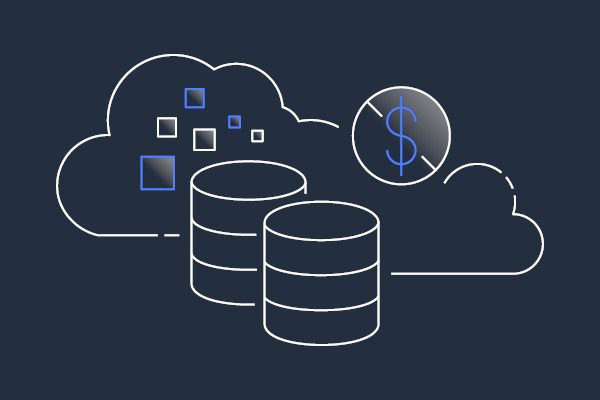
\includegraphics[scale = 0.75]{figs/db-logo-dollar}};","","  % \\uncover\u003c1\u003e{","  % \\draw[comm] (t-bob) -- (db);","  % }","","  % \\uncover\u003c3-\u003e{","  \\draw[comm] (t-alice) -- (t-alice |- isolation.north);","  \\draw[comm] (t-bob) -- (t-bob |- isolation.north);","  \\draw[comm] (t-carol) -- (t-carol |- isolation.north);","  \\draw[comm] (isolation) -- (isolation |- db.north);","  % }","\\end{tikzpicture}"],"stylingDirectives":null,"colorizedLines":["\u003cspan class=\"pl-c\"\u003e\u003cspan class=\"pl-c\"\u003e%\u003c/span\u003e isolation-intro-write-skew-tikz.tex\u003c/span\u003e","","\u003cspan class=\"pl-c1\"\u003e\\begin\u003c/span\u003e{\u003cspan class=\"pl-smi\"\u003etikzpicture\u003c/span\u003e}[","  node distance = 1.5cm and 1.5cm,","  txn/.style = {draw, inner sep = 3pt, align = left},","  comm/.style = {arrows = {Stealth-Stealth}, ultra thick, purple}]","","  \u003cspan class=\"pl-c\"\u003e\u003cspan class=\"pl-c\"\u003e%\u003c/span\u003e \\uncover\u0026lt;2-\u0026gt;{\u003c/span\u003e","  \u003cspan class=\"pl-c1\"\u003e\\node\u003c/span\u003e[txn] (t-alice)","    {\u003cspan class=\"pl-s\"\u003e\u003cspan class=\"pl-pds\"\u003e$\u003c/span\u003ex_{1} \u003cspan class=\"pl-c1\"\u003e\\gets\u003c/span\u003e \u003cspan class=\"pl-c1\"\u003e\\readevent\u003c/span\u003e(\u003cspan class=\"pl-c1\"\u003e\\acctone\u003c/span\u003e)\u003cspan class=\"pl-pds\"\u003e$\u003c/span\u003e\u003c/span\u003e\u003cspan class=\"pl-c1\"\u003e\\\\\u003c/span\u003e[2pt]","     \u003cspan class=\"pl-s\"\u003e\u003cspan class=\"pl-pds\"\u003e$\u003c/span\u003ex_{2} \u003cspan class=\"pl-c1\"\u003e\\gets\u003c/span\u003e \u003cspan class=\"pl-c1\"\u003e\\readevent\u003c/span\u003e(\u003cspan class=\"pl-c1\"\u003e\\accttwo\u003c/span\u003e)\u003cspan class=\"pl-pds\"\u003e$\u003c/span\u003e\u003c/span\u003e\u003cspan class=\"pl-c1\"\u003e\\\\\u003c/span\u003e[2pt]","     \u003cspan class=\"pl-s\"\u003e\u003cspan class=\"pl-pds\"\u003e$\u003c/span\u003e\u003cspan class=\"pl-c1\"\u003e\\text\u003c/span\u003e{\u003cspan class=\"pl-c1\"\u003e\\bf\u003c/span\u003e if}\u003cspan class=\"pl-cce\"\u003e\\;\u003c/span\u003e x_{1} + x_{2} \u0026gt; \u003cspan class=\"pl-c1\"\u003e100\u003c/span\u003e\u003cspan class=\"pl-pds\"\u003e$\u003c/span\u003e\u003c/span\u003e \u003cspan class=\"pl-c1\"\u003e\\\\\u003c/span\u003e[2pt]","     \u003cspan class=\"pl-s\"\u003e\u003cspan class=\"pl-pds\"\u003e$\u003c/span\u003e\u003cspan class=\"pl-c1\"\u003e\\quad\u003c/span\u003e \u003cspan class=\"pl-c1\"\u003e\\red\u003c/span\u003e{x_{1} \u003cspan class=\"pl-c1\"\u003e\\gets\u003c/span\u003e x_{1} - 100}\u003cspan class=\"pl-pds\"\u003e$\u003c/span\u003e\u003c/span\u003e \u003cspan class=\"pl-c1\"\u003e\\\\\u003c/span\u003e[2pt]","     \u003cspan class=\"pl-s\"\u003e\u003cspan class=\"pl-pds\"\u003e$\u003c/span\u003e\u003cspan class=\"pl-c1\"\u003e\\quad\u003c/span\u003e \u003cspan class=\"pl-c1\"\u003e\\writeevent\u003c/span\u003e(\u003cspan class=\"pl-c1\"\u003e\\acctone\u003c/span\u003e, x_{1})\u003cspan class=\"pl-pds\"\u003e$\u003c/span\u003e\u003c/span\u003e};","  \u003cspan class=\"pl-c\"\u003e\u003cspan class=\"pl-c\"\u003e%\u003c/span\u003e }\u003c/span\u003e","","  \u003cspan class=\"pl-c1\"\u003e\\node\u003c/span\u003e[txn, right = of t-alice] (t-bob)","    {\u003cspan class=\"pl-s\"\u003e\u003cspan class=\"pl-pds\"\u003e$\u003c/span\u003ex_{1} \u003cspan class=\"pl-c1\"\u003e\\gets\u003c/span\u003e \u003cspan class=\"pl-c1\"\u003e\\readevent\u003c/span\u003e(\u003cspan class=\"pl-c1\"\u003e\\acctone\u003c/span\u003e)\u003cspan class=\"pl-pds\"\u003e$\u003c/span\u003e\u003c/span\u003e\u003cspan class=\"pl-c1\"\u003e\\\\\u003c/span\u003e[2pt]","     \u003cspan class=\"pl-s\"\u003e\u003cspan class=\"pl-pds\"\u003e$\u003c/span\u003ex_{2} \u003cspan class=\"pl-c1\"\u003e\\gets\u003c/span\u003e \u003cspan class=\"pl-c1\"\u003e\\readevent\u003c/span\u003e(\u003cspan class=\"pl-c1\"\u003e\\accttwo\u003c/span\u003e)\u003cspan class=\"pl-pds\"\u003e$\u003c/span\u003e\u003c/span\u003e\u003cspan class=\"pl-c1\"\u003e\\\\\u003c/span\u003e[2pt]","     \u003cspan class=\"pl-s\"\u003e\u003cspan class=\"pl-pds\"\u003e$\u003c/span\u003e\u003cspan class=\"pl-c1\"\u003e\\text\u003c/span\u003e{\u003cspan class=\"pl-c1\"\u003e\\bf\u003c/span\u003e if}\u003cspan class=\"pl-cce\"\u003e\\;\u003c/span\u003e x_{1} + x_{2} \u0026gt; \u003cspan class=\"pl-c1\"\u003e100\u003c/span\u003e\u003cspan class=\"pl-pds\"\u003e$\u003c/span\u003e\u003c/span\u003e \u003cspan class=\"pl-c1\"\u003e\\\\\u003c/span\u003e[2pt]","     \u003cspan class=\"pl-s\"\u003e\u003cspan class=\"pl-pds\"\u003e$\u003c/span\u003e\u003cspan class=\"pl-c1\"\u003e\\quad\u003c/span\u003e \u003cspan class=\"pl-c1\"\u003e\\red\u003c/span\u003e{x_{2} \u003cspan class=\"pl-c1\"\u003e\\gets\u003c/span\u003e x_{2} - 100}\u003cspan class=\"pl-pds\"\u003e$\u003c/span\u003e\u003c/span\u003e \u003cspan class=\"pl-c1\"\u003e\\\\\u003c/span\u003e[2pt]","     \u003cspan class=\"pl-s\"\u003e\u003cspan class=\"pl-pds\"\u003e$\u003c/span\u003e\u003cspan class=\"pl-c1\"\u003e\\quad\u003c/span\u003e \u003cspan class=\"pl-c1\"\u003e\\writeevent\u003c/span\u003e(\u003cspan class=\"pl-c1\"\u003e\\accttwo\u003c/span\u003e, x_{2})\u003cspan class=\"pl-pds\"\u003e$\u003c/span\u003e\u003c/span\u003e};","","  \u003cspan class=\"pl-c\"\u003e\u003cspan class=\"pl-c\"\u003e%\u003c/span\u003e \\uncover\u0026lt;2-\u0026gt;{\u003c/span\u003e","  \u003cspan class=\"pl-c1\"\u003e\\node\u003c/span\u003e[txn, right = of t-bob] (t-carol)","    {\u003cspan class=\"pl-s\"\u003e\u003cspan class=\"pl-pds\"\u003e$\u003c/span\u003ex_{1} \u003cspan class=\"pl-c1\"\u003e\\gets\u003c/span\u003e \u003cspan class=\"pl-c1\"\u003e\\readevent\u003c/span\u003e(\u003cspan class=\"pl-c1\"\u003e\\acctone\u003c/span\u003e)\u003cspan class=\"pl-pds\"\u003e$\u003c/span\u003e\u003c/span\u003e\u003cspan class=\"pl-c1\"\u003e\\\\\u003c/span\u003e[2pt]","     \u003cspan class=\"pl-s\"\u003e\u003cspan class=\"pl-pds\"\u003e$\u003c/span\u003ex_{2} \u003cspan class=\"pl-c1\"\u003e\\gets\u003c/span\u003e \u003cspan class=\"pl-c1\"\u003e\\readevent\u003c/span\u003e(\u003cspan class=\"pl-c1\"\u003e\\accttwo\u003c/span\u003e)\u003cspan class=\"pl-pds\"\u003e$\u003c/span\u003e\u003c/span\u003e};","  \u003cspan class=\"pl-c\"\u003e\u003cspan class=\"pl-c\"\u003e%\u003c/span\u003e }\u003c/span\u003e","","  \u003cspan class=\"pl-c\"\u003e\u003cspan class=\"pl-c\"\u003e%\u003c/span\u003e \\uncover\u0026lt;3-\u0026gt;{\u003c/span\u003e","  \u003cspan class=\"pl-c1\"\u003e\\node\u003c/span\u003e[draw, fill = yellow!50, below = of t-bob, font = \u003cspan class=\"pl-c1\"\u003e\\large\u003c/span\u003e,","    inner sep = 8pt] (isolation)","    {{Isolation Level (aka Transactional Consistency Model)}};","  \u003cspan class=\"pl-c\"\u003e\u003cspan class=\"pl-c\"\u003e%\u003c/span\u003e }\u003c/span\u003e","","  \u003cspan class=\"pl-c1\"\u003e\\node\u003c/span\u003e[below = of isolation,","    label = {[label distance = 5pt]above : {\u003cspan class=\"pl-c1\"\u003e\\large\u003c/span\u003e \u003cspan class=\"pl-s\"\u003e\u003cspan class=\"pl-pds\"\u003e$\u003c/span\u003e\u003cspan class=\"pl-c1\"\u003e\\acctone\u003c/span\u003e = \u003cspan class=\"pl-c1\"\u003e\\accttwo\u003c/span\u003e = \u003cspan class=\"pl-c1\"\u003e60\u003c/span\u003e\u003cspan class=\"pl-pds\"\u003e$\u003c/span\u003e\u003c/span\u003e}}] (db)","    {\u003cspan class=\"pl-c1\"\u003e\\includegraphics\u003c/span\u003e[scale = 0.75]{figs/db-logo-dollar}};","","  \u003cspan class=\"pl-c\"\u003e\u003cspan class=\"pl-c\"\u003e%\u003c/span\u003e \\uncover\u0026lt;1\u0026gt;{\u003c/span\u003e","  \u003cspan class=\"pl-c\"\u003e\u003cspan class=\"pl-c\"\u003e%\u003c/span\u003e \\draw[comm] (t-bob) -- (db);\u003c/span\u003e","  \u003cspan class=\"pl-c\"\u003e\u003cspan class=\"pl-c\"\u003e%\u003c/span\u003e }\u003c/span\u003e","","  \u003cspan class=\"pl-c\"\u003e\u003cspan class=\"pl-c\"\u003e%\u003c/span\u003e \\uncover\u0026lt;3-\u0026gt;{\u003c/span\u003e","  \u003cspan class=\"pl-c1\"\u003e\\draw\u003c/span\u003e[comm] (t-alice) -- (t-alice |- isolation.north);","  \u003cspan class=\"pl-c1\"\u003e\\draw\u003c/span\u003e[comm] (t-bob) -- (t-bob |- isolation.north);","  \u003cspan class=\"pl-c1\"\u003e\\draw\u003c/span\u003e[comm] (t-carol) -- (t-carol |- isolation.north);","  \u003cspan class=\"pl-c1\"\u003e\\draw\u003c/span\u003e[comm] (isolation) -- (isolation |- db.north);","  \u003cspan class=\"pl-c\"\u003e\u003cspan class=\"pl-c\"\u003e%\u003c/span\u003e }\u003c/span\u003e","\u003cspan class=\"pl-c1\"\u003e\\end\u003c/span\u003e{\u003cspan class=\"pl-smi\"\u003etikzpicture\u003c/span\u003e}"],"csv":null,"csvError":null,"copilotSWEAgentEnabled":true,"dependabotInfo":{"showConfigurationBanner":false,"configFilePath":null,"networkDependabotPath":"/reports-by-hfwei/polysi-vldb2023-report/network/updates","dismissConfigurationNoticePath":"/settings/dismiss-notice/dependabot_configuration_notice","configurationNoticeDismissed":false},"displayName":"isolation-intro-write-skew-tikz.tex","displayUrl":"https://github.com/reports-by-hfwei/polysi-vldb2023-report/blob/main/tikz/isolation-intro-write-skew-tikz.tex?raw=true","headerInfo":{"blobSize":"1.58 KB","deleteTooltip":"Delete this file","editTooltip":"Edit this file","ghDesktopPath":"https://desktop.github.com","isGitLfs":false,"onBranch":true,"shortPath":"9d1f689","siteNavLoginPath":"/login?return_to=https%3A%2F%2Fgithub.com%2Freports-by-hfwei%2Fpolysi-vldb2023-report%2Fblob%2Fmain%2Ftikz%2Fisolation-intro-write-skew-tikz.tex","isCSV":false,"isRichtext":false,"toc":null,"lineInfo":{"truncatedLoc":"50","truncatedSloc":"42"},"mode":"file"},"image":false,"isCodeownersFile":null,"isPlain":false,"isValidLegacyIssueTemplate":false,"issueTemplate":null,"discussionTemplate":null,"language":"TeX","languageID":369,"large":false,"planSupportInfo":{"repoIsFork":null,"repoOwnedByCurrentUser":null,"requestFullPath":"/reports-by-hfwei/polysi-vldb2023-report/blob/main/tikz/isolation-intro-write-skew-tikz.tex","showFreeOrgGatedFeatureMessage":null,"showPlanSupportBanner":null,"upgradeDataAttributes":null,"upgradePath":null},"publishBannersInfo":{"dismissActionNoticePath":"/settings/dismiss-notice/publish_action_from_dockerfile","releasePath":"/reports-by-hfwei/polysi-vldb2023-report/releases/new?marketplace=true","showPublishActionBanner":false},"rawBlobUrl":"https://github.com/reports-by-hfwei/polysi-vldb2023-report/raw/refs/heads/main/tikz/isolation-intro-write-skew-tikz.tex","renderImageOrRaw":false,"richText":null,"renderedFileInfo":null,"shortPath":null,"symbolsEnabled":true,"tabSize":4,"topBannersInfo":{"overridingGlobalFundingFile":false,"globalPreferredFundingPath":null,"showInvalidCitationWarning":false,"citationHelpUrl":"https://docs.github.com/github/creating-cloning-and-archiving-repositories/creating-a-repository-on-github/about-citation-files","actionsOnboardingTip":null},"truncated":false,"viewable":true,"workflowRedirectUrl":null,"symbols":{"timed_out":false,"not_analyzed":true,"symbols":[]}},"copilotInfo":null,"copilotAccessAllowed":true,"modelsAccessAllowed":false,"modelsRepoIntegrationEnabled":false,"isMarketplaceEnabled":true,"csrf_tokens":{"/reports-by-hfwei/polysi-vldb2023-report/branches":{"post":"LZ6dK5lNK_ChBC3W7OahSPruaPp6FlKEBdtnxDcBFiOSiy4W6y2CsWolc8yRoCEQphc0yGGj2KaCAKBtZP0CcA"},"/repos/preferences":{"post":"fSxMoTnlvCFUPdkj38RI7eBLnH7r6kOX9cy6OYT9dmvI-ExZV5f-jrPozzL2jRlR546Ps9OLtf1rVzjV-1cfwg"}}},"title":"polysi-vldb2023-report/tikz/isolation-intro-write-skew-tikz.tex at main · reports-by-hfwei/polysi-vldb2023-report","appPayload":{"helpUrl":"https://docs.github.com","findFileWorkerPath":"/assets-cdn/worker/find-file-worker-9bd411a8e273.js","findInFileWorkerPath":"/assets-cdn/worker/find-in-file-worker-410714137fc9.js","githubDevUrl":"https://github.dev/","enabled_features":{"code_nav_ui_events":false,"react_blob_overlay":true,"accessible_code_button":true}}}</script>
  <div data-target="react-app.reactRoot"><style data-styled="true" data-styled-version="5.3.11">.gISSDQ{width:100%;}/*!sc*/
@media screen and (min-width:544px){.gISSDQ{width:100%;}}/*!sc*/
@media screen and (min-width:768px){.gISSDQ{width:auto;}}/*!sc*/
.birIjn{max-height:100%;height:100%;display:-webkit-box;display:-webkit-flex;display:-ms-flexbox;display:flex;-webkit-flex-direction:column;-ms-flex-direction:column;flex-direction:column;}/*!sc*/
@media screen and (max-width:768px){.birIjn{display:none;}}/*!sc*/
@media screen and (min-width:768px){.birIjn{max-height:100vh;height:100vh;}}/*!sc*/
.jfIeyl{display:-webkit-box;display:-webkit-flex;display:-ms-flexbox;display:flex;width:100%;margin-bottom:16px;-webkit-align-items:center;-webkit-box-align:center;-ms-flex-align:center;align-items:center;}/*!sc*/
.kOkWgo{font-size:16px;margin-left:8px;}/*!sc*/
.dPUXSa[data-size="medium"][data-no-visuals]{border-top-left-radius:0;border-bottom-left-radius:0;}/*!sc*/
@media screen and (max-width:768px){.jLLPHh{display:none;}}/*!sc*/
.bHLmSv{position:absolute;inset:0 -2px;cursor:col-resize;background-color:transparent;-webkit-transition-delay:0.1s;transition-delay:0.1s;}/*!sc*/
.bHLmSv:hover{background-color:var(--bgColor-neutral-muted,var(--color-neutral-muted,rgba(175,184,193,0.2)));}/*!sc*/
.leYMvG{margin-left:auto;margin-right:auto;-webkit-flex-direction:column;-ms-flex-direction:column;flex-direction:column;padding-bottom:40px;max-width:100%;margin-top:0;}/*!sc*/
.KMPzq{display:inherit;}/*!sc*/
.cEytCf{display:-webkit-box;display:-webkit-flex;display:-ms-flexbox;display:flex;-webkit-flex-direction:row;-ms-flex-direction:row;flex-direction:row;font-size:16px;min-width:0;-webkit-flex-shrink:1;-ms-flex-negative:1;flex-shrink:1;-webkit-flex-wrap:wrap;-ms-flex-wrap:wrap;flex-wrap:wrap;max-width:100%;-webkit-align-items:center;-webkit-box-align:center;-ms-flex-align:center;align-items:center;}/*!sc*/
.fzFXnm{max-width:100%;}/*!sc*/
.iMnkmv{max-width:100%;list-style:none;display:inline-block;}/*!sc*/
.ghzDag{display:inline-block;max-width:100%;}/*!sc*/
.kHuKdh{font-weight:600;}/*!sc*/
.hzJBof{padding-left:4px;padding-right:4px;font-weight:400;color:var(--fgColor-muted,var(--color-fg-muted,#656d76));font-size:16px;}/*!sc*/
.kgiVEz{font-weight:400;}/*!sc*/
.jGhzSQ{font-weight:600;display:inline-block;max-width:100%;font-size:16px;}/*!sc*/
.fjrFuv[data-size="medium"][data-no-visuals]{display:none;}/*!sc*/
.gUkoLg{-webkit-box-pack:center;-webkit-justify-content:center;-ms-flex-pack:center;justify-content:center;}/*!sc*/
.dJxjrT{margin-left:16px;margin-right:16px;}/*!sc*/
.ldRxiI{display:-webkit-box;display:-webkit-flex;display:-ms-flexbox;display:flex;-webkit-flex-direction:row;-ms-flex-direction:row;flex-direction:row;}/*!sc*/
.fVkfyA{width:100%;height:-webkit-fit-content;height:-moz-fit-content;height:fit-content;min-width:0;margin-right:0;}/*!sc*/
.gNAmSV{height:40px;padding-left:4px;padding-bottom:16px;}/*!sc*/
.jdLMhu{top:0px;z-index:4;background:var(--bgColor-default,var(--color-canvas-default));position:-webkit-sticky;position:sticky;}/*!sc*/
.hqwSEx{display:none;min-width:0;padding-top:8px;padding-bottom:8px;}/*!sc*/
.fHind{display:-webkit-box;display:-webkit-flex;display:-ms-flexbox;display:flex;-webkit-flex-direction:row;-ms-flex-direction:row;flex-direction:row;font-size:14px;min-width:0;-webkit-flex-shrink:1;-ms-flex-negative:1;flex-shrink:1;-webkit-flex-wrap:wrap;-ms-flex-wrap:wrap;flex-wrap:wrap;max-width:100%;-webkit-align-items:center;-webkit-box-align:center;-ms-flex-align:center;align-items:center;}/*!sc*/
.oDtgN{padding-left:4px;padding-right:4px;font-weight:400;color:var(--fgColor-muted,var(--color-fg-muted,#656d76));font-size:14px;}/*!sc*/
.dnZoUW{font-weight:600;display:inline-block;max-width:100%;font-size:14px;}/*!sc*/
.gFKFyc{border-radius:6px 6px 0px 0px;}/*!sc*/
.lefpaC linkButtonSx:hover:not([disabled]){-webkit-text-decoration:none;text-decoration:none;}/*!sc*/
.lefpaC linkButtonSx:focus:not([disabled]){-webkit-text-decoration:none;text-decoration:none;}/*!sc*/
.lefpaC linkButtonSx:active:not([disabled]){-webkit-text-decoration:none;text-decoration:none;}/*!sc*/
.ivobqY[data-size="small"][data-no-visuals]{border-top-left-radius:0;border-bottom-left-radius:0;}/*!sc*/
.iCOsHh[data-size="small"][data-no-visuals]:hover:not([disabled]){-webkit-text-decoration:none;text-decoration:none;}/*!sc*/
.iCOsHh[data-size="small"][data-no-visuals]:focus:not([disabled]){-webkit-text-decoration:none;text-decoration:none;}/*!sc*/
.iCOsHh[data-size="small"][data-no-visuals]:active:not([disabled]){-webkit-text-decoration:none;text-decoration:none;}/*!sc*/
.hGyMdv{border:1px solid;border-top:none;border-color:var(--borderColor-default,var(--color-border-default,#d0d7de));border-radius:0px 0px 6px 6px;min-width:273px;}/*!sc*/
.dceWRL{background-color:var(--bgColor-default,var(--color-canvas-default));border:0px;border-width:0;border-radius:0px 0px 6px 6px;padding:0;min-width:0;margin-top:46px;}/*!sc*/
.dGXHv{display:-webkit-box;display:-webkit-flex;display:-ms-flexbox;display:flex;-webkit-flex:1;-ms-flex:1;flex:1;padding-top:8px;padding-bottom:8px;-webkit-flex-direction:column;-ms-flex-direction:column;flex-direction:column;-webkit-box-pack:justify;-webkit-justify-content:space-between;-ms-flex-pack:justify;justify-content:space-between;min-width:0;position:relative;}/*!sc*/
.bpDFns{position:relative;}/*!sc*/
.iJOeCH{-webkit-flex:1;-ms-flex:1;flex:1;position:relative;min-width:0;}/*!sc*/
.glDApP{tab-size:4;isolation:isolate;position:relative;overflow:auto;max-width:unset;}/*!sc*/
.cCoXib{position:fixed;top:0;right:0;height:100%;width:15px;-webkit-transition:-webkit-transform 0.3s;-webkit-transition:transform 0.3s;transition:transform 0.3s;z-index:1;}/*!sc*/
.cCoXib:hover{-webkit-transform:scaleX(1.5);-ms-transform:scaleX(1.5);transform:scaleX(1.5);}/*!sc*/
data-styled.g1[id="Box-sc-g0xbh4-0"]{content:"gISSDQ,birIjn,jfIeyl,kOkWgo,dPUXSa,jLLPHh,bHLmSv,leYMvG,KMPzq,cEytCf,fzFXnm,iMnkmv,ghzDag,kHuKdh,hzJBof,kgiVEz,jGhzSQ,fjrFuv,gUkoLg,dJxjrT,ldRxiI,fVkfyA,gNAmSV,jdLMhu,hqwSEx,fHind,oDtgN,dnZoUW,gFKFyc,lefpaC,ivobqY,iCOsHh,hGyMdv,dceWRL,dGXHv,bpDFns,iJOeCH,glDApP,cCoXib,"}/*!sc*/
.hWlpPn{position:relative;display:inline-block;}/*!sc*/
.hWlpPn::after{position:absolute;z-index:1000000;display:none;padding:0.5em 0.75em;font:normal normal 11px/1.5 -apple-system,BlinkMacSystemFont,"Segoe UI","Noto Sans",Helvetica,Arial,sans-serif,"Apple Color Emoji","Segoe UI Emoji";-webkit-font-smoothing:subpixel-antialiased;color:var(--tooltip-fgColor,var(--fgColor-onEmphasis,var(--color-fg-on-emphasis,#ffffff)));text-align:center;-webkit-text-decoration:none;text-decoration:none;text-shadow:none;text-transform:none;-webkit-letter-spacing:normal;-moz-letter-spacing:normal;-ms-letter-spacing:normal;letter-spacing:normal;word-wrap:break-word;white-space:pre;pointer-events:none;content:attr(aria-label);background:var(--tooltip-bgColor,var(--bgColor-emphasis,var(--color-neutral-emphasis-plus,#24292f)));border-radius:6px;opacity:0;}/*!sc*/
@-webkit-keyframes tooltip-appear{from{opacity:0;}to{opacity:1;}}/*!sc*/
@keyframes tooltip-appear{from{opacity:0;}to{opacity:1;}}/*!sc*/
.hWlpPn:hover::after,.hWlpPn:active::after,.hWlpPn:focus::after,.hWlpPn:focus-within::after{display:inline-block;-webkit-text-decoration:none;text-decoration:none;-webkit-animation-name:tooltip-appear;animation-name:tooltip-appear;-webkit-animation-duration:0.1s;animation-duration:0.1s;-webkit-animation-fill-mode:forwards;animation-fill-mode:forwards;-webkit-animation-timing-function:ease-in;animation-timing-function:ease-in;-webkit-animation-delay:0s;animation-delay:0s;}/*!sc*/
.hWlpPn.tooltipped-no-delay:hover::after,.hWlpPn.tooltipped-no-delay:active::after,.hWlpPn.tooltipped-no-delay:focus::after,.hWlpPn.tooltipped-no-delay:focus-within::after{-webkit-animation-delay:0s;animation-delay:0s;}/*!sc*/
.hWlpPn.tooltipped-multiline:hover::after,.hWlpPn.tooltipped-multiline:active::after,.hWlpPn.tooltipped-multiline:focus::after,.hWlpPn.tooltipped-multiline:focus-within::after{display:table-cell;}/*!sc*/
.hWlpPn.tooltipped-s::after,.hWlpPn.tooltipped-se::after,.hWlpPn.tooltipped-sw::after{top:100%;right:50%;margin-top:6px;}/*!sc*/
.hWlpPn.tooltipped-se::after{right:auto;left:50%;margin-left:-16px;}/*!sc*/
.hWlpPn.tooltipped-sw::after{margin-right:-16px;}/*!sc*/
.hWlpPn.tooltipped-n::after,.hWlpPn.tooltipped-ne::after,.hWlpPn.tooltipped-nw::after{right:50%;bottom:100%;margin-bottom:6px;}/*!sc*/
.hWlpPn.tooltipped-ne::after{right:auto;left:50%;margin-left:-16px;}/*!sc*/
.hWlpPn.tooltipped-nw::after{margin-right:-16px;}/*!sc*/
.hWlpPn.tooltipped-s::after,.hWlpPn.tooltipped-n::after{-webkit-transform:translateX(50%);-ms-transform:translateX(50%);transform:translateX(50%);}/*!sc*/
.hWlpPn.tooltipped-w::after{right:100%;bottom:50%;margin-right:6px;-webkit-transform:translateY(50%);-ms-transform:translateY(50%);transform:translateY(50%);}/*!sc*/
.hWlpPn.tooltipped-e::after{bottom:50%;left:100%;margin-left:6px;-webkit-transform:translateY(50%);-ms-transform:translateY(50%);transform:translateY(50%);}/*!sc*/
.hWlpPn.tooltipped-multiline::after{width:-webkit-max-content;width:-moz-max-content;width:max-content;max-width:250px;word-wrap:break-word;white-space:pre-line;border-collapse:separate;}/*!sc*/
.hWlpPn.tooltipped-multiline.tooltipped-s::after,.hWlpPn.tooltipped-multiline.tooltipped-n::after{right:auto;left:50%;-webkit-transform:translateX(-50%);-ms-transform:translateX(-50%);transform:translateX(-50%);}/*!sc*/
.hWlpPn.tooltipped-multiline.tooltipped-w::after,.hWlpPn.tooltipped-multiline.tooltipped-e::after{right:100%;}/*!sc*/
.hWlpPn.tooltipped-align-right-2::after{right:0;margin-right:0;}/*!sc*/
.hWlpPn.tooltipped-align-left-2::after{left:0;margin-left:0;}/*!sc*/
data-styled.g4[id="Tooltip__TooltipBase-sc-17tf59c-0"]{content:"hWlpPn,"}/*!sc*/
</style><meta data-hydrostats="publish"/> <!-- --> <!-- --> <button hidden="" data-testid="header-permalink-button" data-hotkey-scope="read-only-cursor-text-area"></button><button hidden=""></button><div><div style="--spacing:var(--spacing-none)" class="prc-PageLayout-PageLayoutRoot-1zlEO"><div class="prc-PageLayout-PageLayoutWrapper-s2ao4" data-width="full"><div class="prc-PageLayout-PageLayoutContent-jzDMn"><div tabindex="0" class="Box-sc-g0xbh4-0 gISSDQ"><div class="prc-PageLayout-PaneWrapper-nGO0U ReposFileTreePane-module__Pane--D26Sw ReposFileTreePane-module__HidePaneWithTreeOverlay--CJn2n" style="--offset-header:0px;--spacing-row:var(--spacing-none);--spacing-column:var(--spacing-none)" data-is-hidden="false" data-position="start" data-sticky="true"><div class="prc-PageLayout-HorizontalDivider-CYLp5 prc-PageLayout-PaneHorizontalDivider-4exOb" data-variant="none" data-position="start" style="--spacing-divider:var(--spacing-none);--spacing:var(--spacing-none)"></div><div class="prc-PageLayout-Pane-Vl5LI" data-resizable="true" style="--spacing:var(--spacing-none);--pane-min-width:256px;--pane-max-width:calc(100vw - var(--pane-max-width-diff));--pane-width-size:var(--pane-width-large);--pane-width:320px"><div class="react-tree-pane-contents-3-panel"><div id="repos-file-tree" class="Box-sc-g0xbh4-0 birIjn"><div class="ReposFileTreePane-module__Box_1--ZT_4S"><div class="Box-sc-g0xbh4-0 jfIeyl"><h2 class="use-tree-pane-module__Heading--iI_ad prc-Heading-Heading-6CmGO"><button type="button" aria-label="Expand file tree" data-testid="expand-file-tree-button-mobile" class="prc-Button-ButtonBase-c50BI ExpandFileTreeButton-module__Button_1--g8F6Q" data-loading="false" data-size="medium" data-variant="invisible" aria-describedby=":Rl6mplab:-loading-announcement"><span data-component="buttonContent" data-align="center" class="prc-Button-ButtonContent-HKbr-"><span data-component="leadingVisual" class="prc-Button-Visual-2epfX prc-Button-VisualWrap-Db-eB"><svg aria-hidden="true" focusable="false" class="octicon octicon-arrow-left" viewBox="0 0 16 16" width="16" height="16" fill="currentColor" display="inline-block" overflow="visible" style="vertical-align:text-bottom"><path d="M7.78 12.53a.75.75 0 0 1-1.06 0L2.47 8.28a.75.75 0 0 1 0-1.06l4.25-4.25a.751.751 0 0 1 1.042.018.751.751 0 0 1 .018 1.042L4.81 7h7.44a.75.75 0 0 1 0 1.5H4.81l2.97 2.97a.75.75 0 0 1 0 1.06Z"></path></svg></span><span data-component="text" class="prc-Button-Label-pTQ3x">Files</span></span></button><button data-component="IconButton" type="button" data-testid="collapse-file-tree-button" aria-expanded="true" aria-controls="repos-file-tree" class="prc-Button-ButtonBase-c50BI position-relative ExpandFileTreeButton-module__expandButton--oKI1R ExpandFileTreeButton-module__filesButtonBreakpoint--03FKA fgColor-muted prc-Button-IconButton-szpyj" data-loading="false" data-no-visuals="true" data-size="medium" data-variant="invisible" aria-describedby=":R756mplab:-loading-announcement" aria-labelledby=":R156mplab:"><svg aria-hidden="true" focusable="false" class="octicon octicon-sidebar-expand" viewBox="0 0 16 16" width="16" height="16" fill="currentColor" display="inline-block" overflow="visible" style="vertical-align:text-bottom"><path d="m4.177 7.823 2.396-2.396A.25.25 0 0 1 7 5.604v4.792a.25.25 0 0 1-.427.177L4.177 8.177a.25.25 0 0 1 0-.354Z"></path><path d="M0 1.75C0 .784.784 0 1.75 0h12.5C15.216 0 16 .784 16 1.75v12.5A1.75 1.75 0 0 1 14.25 16H1.75A1.75 1.75 0 0 1 0 14.25Zm1.75-.25a.25.25 0 0 0-.25.25v12.5c0 .138.112.25.25.25H9.5v-13Zm12.5 13a.25.25 0 0 0 .25-.25V1.75a.25.25 0 0 0-.25-.25H11v13Z"></path></svg></button><span class="prc-TooltipV2-Tooltip-cYMVY" data-direction="se" aria-hidden="true" id=":R156mplab:">Collapse file tree</span><button hidden="" data-testid="" data-hotkey-scope="read-only-cursor-text-area"></button></h2><h2 class="Box-sc-g0xbh4-0 kOkWgo prc-Heading-Heading-6CmGO">Files</h2></div><div class="ReposFileTreePane-module__Box_2--RgzGf"><div class="ReposFileTreePane-module__Box_3--XDLn8"><button style="min-width:0" type="button" aria-haspopup="true" aria-expanded="false" tabindex="0" aria-label="main branch" data-testid="anchor-button" class="prc-Button-ButtonBase-c50BI react-repos-tree-pane-ref-selector width-full ref-selector-class RefSelectorAnchoredOverlay-module__RefSelectorOverlayBtn--D34zl" data-loading="false" data-size="medium" data-variant="default" aria-describedby="ref-picker-repos-header-ref-selector-loading-announcement" id="ref-picker-repos-header-ref-selector"><span data-component="buttonContent" data-align="center" class="prc-Button-ButtonContent-HKbr-"><span data-component="text" class="prc-Button-Label-pTQ3x"><div class="RefSelectorAnchoredOverlay-module__RefSelectorOverlayContainer--mCbv8"><div class="RefSelectorAnchoredOverlay-module__RefSelectorOverlayHeader--D4cnZ"><svg aria-hidden="true" focusable="false" class="octicon octicon-git-branch" viewBox="0 0 16 16" width="16" height="16" fill="currentColor" display="inline-block" overflow="visible" style="vertical-align:text-bottom"><path d="M9.5 3.25a2.25 2.25 0 1 1 3 2.122V6A2.5 2.5 0 0 1 10 8.5H6a1 1 0 0 0-1 1v1.128a2.251 2.251 0 1 1-1.5 0V5.372a2.25 2.25 0 1 1 1.5 0v1.836A2.493 2.493 0 0 1 6 7h4a1 1 0 0 0 1-1v-.628A2.25 2.25 0 0 1 9.5 3.25Zm-6 0a.75.75 0 1 0 1.5 0 .75.75 0 0 0-1.5 0Zm8.25-.75a.75.75 0 1 0 0 1.5.75.75 0 0 0 0-1.5ZM4.25 12a.75.75 0 1 0 0 1.5.75.75 0 0 0 0-1.5Z"></path></svg></div><div class="ref-selector-button-text-container RefSelectorAnchoredOverlay-module__RefSelectorBtnTextContainer--yO402"><span class="RefSelectorAnchoredOverlay-module__RefSelectorText--bxVhQ"> <!-- -->main</span></div></div></span><span data-component="trailingVisual" class="prc-Button-Visual-2epfX prc-Button-VisualWrap-Db-eB"><svg aria-hidden="true" focusable="false" class="octicon octicon-triangle-down" viewBox="0 0 16 16" width="16" height="16" fill="currentColor" display="inline-block" overflow="visible" style="vertical-align:text-bottom"><path d="m4.427 7.427 3.396 3.396a.25.25 0 0 0 .354 0l3.396-3.396A.25.25 0 0 0 11.396 7H4.604a.25.25 0 0 0-.177.427Z"></path></svg></span></span></button><button hidden="" data-hotkey-scope="read-only-cursor-text-area"></button></div><div class="ReposFileTreePane-module__Box_4--TLAAU"><a data-component="IconButton" type="button" class="prc-Button-ButtonBase-c50BI ReposFileTreePane-module__IconButton--fpuBk prc-Button-IconButton-szpyj" data-loading="false" data-no-visuals="true" data-size="medium" data-variant="default" aria-describedby=":R6q6mplab:-loading-announcement" aria-labelledby=":Rq6mplab:" href="/reports-by-hfwei/polysi-vldb2023-report/new/main/tikz" data-discover="true"><svg aria-hidden="true" focusable="false" class="octicon octicon-plus" viewBox="0 0 16 16" width="16" height="16" fill="currentColor" display="inline-block" overflow="visible" style="vertical-align:text-bottom"><path d="M7.75 2a.75.75 0 0 1 .75.75V7h4.25a.75.75 0 0 1 0 1.5H8.5v4.25a.75.75 0 0 1-1.5 0V8.5H2.75a.75.75 0 0 1 0-1.5H7V2.75A.75.75 0 0 1 7.75 2Z"></path></svg></a><span class="prc-TooltipV2-Tooltip-cYMVY" data-direction="n" aria-hidden="true" id=":Rq6mplab:">Add file</span><button data-component="IconButton" type="button" class="Box-sc-g0xbh4-0 dPUXSa prc-Button-ButtonBase-c50BI SearchButton-module__IconButton--kxA3Q prc-Button-IconButton-szpyj" data-loading="false" data-no-visuals="true" data-size="medium" data-variant="default" aria-describedby=":Rra6mplab:-loading-announcement" aria-labelledby=":R3a6mplab:"><svg aria-hidden="true" focusable="false" class="octicon octicon-search" viewBox="0 0 16 16" width="16" height="16" fill="currentColor" display="inline-block" overflow="visible" style="vertical-align:text-bottom"><path d="M10.68 11.74a6 6 0 0 1-7.922-8.982 6 6 0 0 1 8.982 7.922l3.04 3.04a.749.749 0 0 1-.326 1.275.749.749 0 0 1-.734-.215ZM11.5 7a4.499 4.499 0 1 0-8.997 0A4.499 4.499 0 0 0 11.5 7Z"></path></svg></button><span class="prc-TooltipV2-Tooltip-cYMVY" data-direction="nw" aria-hidden="true" id=":R3a6mplab:">Search this repository</span><button hidden="" data-testid="" data-hotkey-scope="read-only-cursor-text-area"></button></div></div></div><div class="Box-sc-g0xbh4-0 jLLPHh ReposFileTreePane-module__FileResultsList--YEf_n FileResultsList-module__Box_1--b75fu"><span class="FileResultsList-module__FilesSearchBox--fSAh3 FilesSearchBox-module__TextInput--Rvr17 TextInput-wrapper prc-components-TextInputWrapper-i1ofR prc-components-TextInputBaseWrapper-ueK9q" data-leading-visual="true" data-trailing-visual="true" aria-busy="false"><span class="TextInput-icon" id=":R5amplab:" aria-hidden="true"><svg aria-hidden="true" focusable="false" class="octicon octicon-search" viewBox="0 0 16 16" width="16" height="16" fill="currentColor" display="inline-block" overflow="visible" style="vertical-align:text-bottom"><path d="M10.68 11.74a6 6 0 0 1-7.922-8.982 6 6 0 0 1 8.982 7.922l3.04 3.04a.749.749 0 0 1-.326 1.275.749.749 0 0 1-.734-.215ZM11.5 7a4.499 4.499 0 1 0-8.997 0A4.499 4.499 0 0 0 11.5 7Z"></path></svg></span><input type="text" aria-label="Go to file" role="combobox" aria-controls="file-results-list" aria-expanded="false" aria-haspopup="dialog" autoCorrect="off" spellcheck="false" placeholder="Go to file" aria-describedby=":R5amplab: :R5amplabH1:" data-component="input" class="prc-components-Input-Ic-y8" value=""/><span class="TextInput-icon" id=":R5amplabH1:" aria-hidden="true"><div class="FilesSearchBox-module__Box--QJMeO"><kbd>t</kbd></div></span></span></div><button hidden="" data-testid="" data-hotkey-scope="read-only-cursor-text-area"></button><button hidden=""></button><div class="Box-sc-g0xbh4-0 jLLPHh ReposFileTreePane-module__Box_5--cckih"><div class="react-tree-show-tree-items"><div class="ReposFileTreeView-module__Box--bDodO" data-testid="repos-file-tree-container"><nav aria-label="File Tree Navigation"><span class="prc-src-InternalVisuallyHidden-nlR9R" role="status" aria-live="polite" aria-atomic="true"></span><ul role="tree" aria-label="Files" data-truncate-text="true" class="prc-TreeView-TreeViewRootUlStyles-eZtxW"><li class="PRIVATE_TreeView-item prc-TreeView-TreeViewItem-ShJr0" tabindex="0" id="figs-item" role="treeitem" aria-labelledby=":R3pimplab:" aria-describedby=":R3pimplabH1:" aria-level="1" aria-expanded="false" aria-selected="false"><div class="PRIVATE_TreeView-item-container prc-TreeView-TreeViewItemContainer--2Rkn" style="--level:1;content-visibility:auto;contain-intrinsic-size:auto 2rem"><div style="grid-area:spacer;display:flex"><div style="width:100%;display:flex"></div></div><div class="PRIVATE_TreeView-item-toggle PRIVATE_TreeView-item-toggle--hover PRIVATE_TreeView-item-toggle--end prc-TreeView-TreeViewItemToggle-gWUdE prc-TreeView-TreeViewItemToggleHover-nEgP- prc-TreeView-TreeViewItemToggleEnd-t-AEB"><svg aria-hidden="true" focusable="false" class="octicon octicon-chevron-right" viewBox="0 0 12 12" width="12" height="12" fill="currentColor" display="inline-block" overflow="visible" style="vertical-align:text-bottom"><path d="M4.7 10c-.2 0-.4-.1-.5-.2-.3-.3-.3-.8 0-1.1L6.9 6 4.2 3.3c-.3-.3-.3-.8 0-1.1.3-.3.8-.3 1.1 0l3.3 3.2c.3.3.3.8 0 1.1L5.3 9.7c-.2.2-.4.3-.6.3Z"></path></svg></div><div id=":R3pimplab:" class="PRIVATE_TreeView-item-content prc-TreeView-TreeViewItemContent-f0r0b"><div class="PRIVATE_VisuallyHidden prc-TreeView-TreeViewVisuallyHidden-4-mPv" aria-hidden="true" id=":R3pimplabH1:"></div><div class="PRIVATE_TreeView-item-visual prc-TreeView-TreeViewItemVisual-dRlGq" aria-hidden="true"><div class="PRIVATE_TreeView-directory-icon prc-TreeView-TreeViewDirectoryIcon-PHbeP"><svg aria-hidden="true" focusable="false" class="octicon octicon-file-directory-fill" viewBox="0 0 16 16" width="16" height="16" fill="currentColor" display="inline-block" overflow="visible" style="vertical-align:text-bottom"><path d="M1.75 1A1.75 1.75 0 0 0 0 2.75v10.5C0 14.216.784 15 1.75 15h12.5A1.75 1.75 0 0 0 16 13.25v-8.5A1.75 1.75 0 0 0 14.25 3H7.5a.25.25 0 0 1-.2-.1l-.9-1.2C6.07 1.26 5.55 1 5 1H1.75Z"></path></svg></div></div><span class="PRIVATE_TreeView-item-content-text prc-TreeView-TreeViewItemContentText-smZM-"><span>figs</span></span></div></div></li><li class="PRIVATE_TreeView-item prc-TreeView-TreeViewItem-ShJr0" tabindex="0" id="sections-item" role="treeitem" aria-labelledby=":R5pimplab:" aria-describedby=":R5pimplabH1:" aria-level="1" aria-expanded="false" aria-selected="false"><div class="PRIVATE_TreeView-item-container prc-TreeView-TreeViewItemContainer--2Rkn" style="--level:1;content-visibility:auto;contain-intrinsic-size:auto 2rem"><div style="grid-area:spacer;display:flex"><div style="width:100%;display:flex"></div></div><div class="PRIVATE_TreeView-item-toggle PRIVATE_TreeView-item-toggle--hover PRIVATE_TreeView-item-toggle--end prc-TreeView-TreeViewItemToggle-gWUdE prc-TreeView-TreeViewItemToggleHover-nEgP- prc-TreeView-TreeViewItemToggleEnd-t-AEB"><svg aria-hidden="true" focusable="false" class="octicon octicon-chevron-right" viewBox="0 0 12 12" width="12" height="12" fill="currentColor" display="inline-block" overflow="visible" style="vertical-align:text-bottom"><path d="M4.7 10c-.2 0-.4-.1-.5-.2-.3-.3-.3-.8 0-1.1L6.9 6 4.2 3.3c-.3-.3-.3-.8 0-1.1.3-.3.8-.3 1.1 0l3.3 3.2c.3.3.3.8 0 1.1L5.3 9.7c-.2.2-.4.3-.6.3Z"></path></svg></div><div id=":R5pimplab:" class="PRIVATE_TreeView-item-content prc-TreeView-TreeViewItemContent-f0r0b"><div class="PRIVATE_VisuallyHidden prc-TreeView-TreeViewVisuallyHidden-4-mPv" aria-hidden="true" id=":R5pimplabH1:"></div><div class="PRIVATE_TreeView-item-visual prc-TreeView-TreeViewItemVisual-dRlGq" aria-hidden="true"><div class="PRIVATE_TreeView-directory-icon prc-TreeView-TreeViewDirectoryIcon-PHbeP"><svg aria-hidden="true" focusable="false" class="octicon octicon-file-directory-fill" viewBox="0 0 16 16" width="16" height="16" fill="currentColor" display="inline-block" overflow="visible" style="vertical-align:text-bottom"><path d="M1.75 1A1.75 1.75 0 0 0 0 2.75v10.5C0 14.216.784 15 1.75 15h12.5A1.75 1.75 0 0 0 16 13.25v-8.5A1.75 1.75 0 0 0 14.25 3H7.5a.25.25 0 0 1-.2-.1l-.9-1.2C6.07 1.26 5.55 1 5 1H1.75Z"></path></svg></div></div><span class="PRIVATE_TreeView-item-content-text prc-TreeView-TreeViewItemContentText-smZM-"><span>sections</span></span></div></div></li><li class="PRIVATE_TreeView-item prc-TreeView-TreeViewItem-ShJr0" tabindex="0" id="tables-item" role="treeitem" aria-labelledby=":R7pimplab:" aria-describedby=":R7pimplabH1:" aria-level="1" aria-expanded="false" aria-selected="false"><div class="PRIVATE_TreeView-item-container prc-TreeView-TreeViewItemContainer--2Rkn" style="--level:1;content-visibility:auto;contain-intrinsic-size:auto 2rem"><div style="grid-area:spacer;display:flex"><div style="width:100%;display:flex"></div></div><div class="PRIVATE_TreeView-item-toggle PRIVATE_TreeView-item-toggle--hover PRIVATE_TreeView-item-toggle--end prc-TreeView-TreeViewItemToggle-gWUdE prc-TreeView-TreeViewItemToggleHover-nEgP- prc-TreeView-TreeViewItemToggleEnd-t-AEB"><svg aria-hidden="true" focusable="false" class="octicon octicon-chevron-right" viewBox="0 0 12 12" width="12" height="12" fill="currentColor" display="inline-block" overflow="visible" style="vertical-align:text-bottom"><path d="M4.7 10c-.2 0-.4-.1-.5-.2-.3-.3-.3-.8 0-1.1L6.9 6 4.2 3.3c-.3-.3-.3-.8 0-1.1.3-.3.8-.3 1.1 0l3.3 3.2c.3.3.3.8 0 1.1L5.3 9.7c-.2.2-.4.3-.6.3Z"></path></svg></div><div id=":R7pimplab:" class="PRIVATE_TreeView-item-content prc-TreeView-TreeViewItemContent-f0r0b"><div class="PRIVATE_VisuallyHidden prc-TreeView-TreeViewVisuallyHidden-4-mPv" aria-hidden="true" id=":R7pimplabH1:"></div><div class="PRIVATE_TreeView-item-visual prc-TreeView-TreeViewItemVisual-dRlGq" aria-hidden="true"><div class="PRIVATE_TreeView-directory-icon prc-TreeView-TreeViewDirectoryIcon-PHbeP"><svg aria-hidden="true" focusable="false" class="octicon octicon-file-directory-fill" viewBox="0 0 16 16" width="16" height="16" fill="currentColor" display="inline-block" overflow="visible" style="vertical-align:text-bottom"><path d="M1.75 1A1.75 1.75 0 0 0 0 2.75v10.5C0 14.216.784 15 1.75 15h12.5A1.75 1.75 0 0 0 16 13.25v-8.5A1.75 1.75 0 0 0 14.25 3H7.5a.25.25 0 0 1-.2-.1l-.9-1.2C6.07 1.26 5.55 1 5 1H1.75Z"></path></svg></div></div><span class="PRIVATE_TreeView-item-content-text prc-TreeView-TreeViewItemContentText-smZM-"><span>tables</span></span></div></div></li><li class="PRIVATE_TreeView-item prc-TreeView-TreeViewItem-ShJr0" tabindex="0" id="tencent-item" role="treeitem" aria-labelledby=":R9pimplab:" aria-describedby=":R9pimplabH1:" aria-level="1" aria-expanded="false" aria-selected="false"><div class="PRIVATE_TreeView-item-container prc-TreeView-TreeViewItemContainer--2Rkn" style="--level:1;content-visibility:auto;contain-intrinsic-size:auto 2rem"><div style="grid-area:spacer;display:flex"><div style="width:100%;display:flex"></div></div><div class="PRIVATE_TreeView-item-toggle PRIVATE_TreeView-item-toggle--hover PRIVATE_TreeView-item-toggle--end prc-TreeView-TreeViewItemToggle-gWUdE prc-TreeView-TreeViewItemToggleHover-nEgP- prc-TreeView-TreeViewItemToggleEnd-t-AEB"><svg aria-hidden="true" focusable="false" class="octicon octicon-chevron-right" viewBox="0 0 12 12" width="12" height="12" fill="currentColor" display="inline-block" overflow="visible" style="vertical-align:text-bottom"><path d="M4.7 10c-.2 0-.4-.1-.5-.2-.3-.3-.3-.8 0-1.1L6.9 6 4.2 3.3c-.3-.3-.3-.8 0-1.1.3-.3.8-.3 1.1 0l3.3 3.2c.3.3.3.8 0 1.1L5.3 9.7c-.2.2-.4.3-.6.3Z"></path></svg></div><div id=":R9pimplab:" class="PRIVATE_TreeView-item-content prc-TreeView-TreeViewItemContent-f0r0b"><div class="PRIVATE_VisuallyHidden prc-TreeView-TreeViewVisuallyHidden-4-mPv" aria-hidden="true" id=":R9pimplabH1:"></div><div class="PRIVATE_TreeView-item-visual prc-TreeView-TreeViewItemVisual-dRlGq" aria-hidden="true"><div class="PRIVATE_TreeView-directory-icon prc-TreeView-TreeViewDirectoryIcon-PHbeP"><svg aria-hidden="true" focusable="false" class="octicon octicon-file-directory-fill" viewBox="0 0 16 16" width="16" height="16" fill="currentColor" display="inline-block" overflow="visible" style="vertical-align:text-bottom"><path d="M1.75 1A1.75 1.75 0 0 0 0 2.75v10.5C0 14.216.784 15 1.75 15h12.5A1.75 1.75 0 0 0 16 13.25v-8.5A1.75 1.75 0 0 0 14.25 3H7.5a.25.25 0 0 1-.2-.1l-.9-1.2C6.07 1.26 5.55 1 5 1H1.75Z"></path></svg></div></div><span class="PRIVATE_TreeView-item-content-text prc-TreeView-TreeViewItemContentText-smZM-"><span>tencent</span></span></div></div></li><li class="PRIVATE_TreeView-item prc-TreeView-TreeViewItem-ShJr0" tabindex="0" id="tikz-item" role="treeitem" aria-labelledby=":Rbpimplab:" aria-describedby=":RbpimplabH1:" aria-level="1" aria-expanded="true" aria-selected="false"><div class="PRIVATE_TreeView-item-container prc-TreeView-TreeViewItemContainer--2Rkn" style="--level:1;content-visibility:auto;contain-intrinsic-size:auto 2rem"><div style="grid-area:spacer;display:flex"><div style="width:100%;display:flex"></div></div><div class="PRIVATE_TreeView-item-toggle PRIVATE_TreeView-item-toggle--hover PRIVATE_TreeView-item-toggle--end prc-TreeView-TreeViewItemToggle-gWUdE prc-TreeView-TreeViewItemToggleHover-nEgP- prc-TreeView-TreeViewItemToggleEnd-t-AEB"><svg aria-hidden="true" focusable="false" class="octicon octicon-chevron-down" viewBox="0 0 12 12" width="12" height="12" fill="currentColor" display="inline-block" overflow="visible" style="vertical-align:text-bottom"><path d="M6 8.825c-.2 0-.4-.1-.5-.2l-3.3-3.3c-.3-.3-.3-.8 0-1.1.3-.3.8-.3 1.1 0l2.7 2.7 2.7-2.7c.3-.3.8-.3 1.1 0 .3.3.3.8 0 1.1l-3.2 3.2c-.2.2-.4.3-.6.3Z"></path></svg></div><div id=":Rbpimplab:" class="PRIVATE_TreeView-item-content prc-TreeView-TreeViewItemContent-f0r0b"><div class="PRIVATE_VisuallyHidden prc-TreeView-TreeViewVisuallyHidden-4-mPv" aria-hidden="true" id=":RbpimplabH1:"></div><div class="PRIVATE_TreeView-item-visual prc-TreeView-TreeViewItemVisual-dRlGq" aria-hidden="true"><div class="PRIVATE_TreeView-directory-icon prc-TreeView-TreeViewDirectoryIcon-PHbeP"><svg aria-hidden="true" focusable="false" class="octicon octicon-file-directory-open-fill" viewBox="0 0 16 16" width="16" height="16" fill="currentColor" display="inline-block" overflow="visible" style="vertical-align:text-bottom"><path d="M.513 1.513A1.75 1.75 0 0 1 1.75 1h3.5c.55 0 1.07.26 1.4.7l.9 1.2a.25.25 0 0 0 .2.1H13a1 1 0 0 1 1 1v.5H2.75a.75.75 0 0 0 0 1.5h11.978a1 1 0 0 1 .994 1.117L15 13.25A1.75 1.75 0 0 1 13.25 15H1.75A1.75 1.75 0 0 1 0 13.25V2.75c0-.464.184-.91.513-1.237Z"></path></svg></div></div><span class="PRIVATE_TreeView-item-content-text prc-TreeView-TreeViewItemContentText-smZM-"><span>tikz</span></span></div></div><ul role="group" style="list-style:none;padding:0;margin:0" aria-label=""><li class="PRIVATE_TreeView-item prc-TreeView-TreeViewItem-ShJr0" tabindex="0" id="tikz/banking-lost-update-depgraph-theorem-tikz.tex-item" role="treeitem" aria-labelledby=":R5dbpimplab:" aria-describedby=":R5dbpimplabH1:" aria-level="2" aria-selected="false"><div class="PRIVATE_TreeView-item-container prc-TreeView-TreeViewItemContainer--2Rkn" style="--level:2;content-visibility:auto;contain-intrinsic-size:auto 2rem"><div style="grid-area:spacer;display:flex"><div style="width:100%;display:flex"><div class="PRIVATE_TreeView-item-level-line prc-TreeView-TreeViewItemLevelLine-KPSSL"></div></div></div><div id=":R5dbpimplab:" class="PRIVATE_TreeView-item-content prc-TreeView-TreeViewItemContent-f0r0b"><div class="PRIVATE_VisuallyHidden prc-TreeView-TreeViewVisuallyHidden-4-mPv" aria-hidden="true" id=":R5dbpimplabH1:"></div><div class="PRIVATE_TreeView-item-visual prc-TreeView-TreeViewItemVisual-dRlGq" aria-hidden="true"><svg aria-hidden="true" focusable="false" class="octicon octicon-file" viewBox="0 0 16 16" width="16" height="16" fill="currentColor" display="inline-block" overflow="visible" style="vertical-align:text-bottom"><path d="M2 1.75C2 .784 2.784 0 3.75 0h6.586c.464 0 .909.184 1.237.513l2.914 2.914c.329.328.513.773.513 1.237v9.586A1.75 1.75 0 0 1 13.25 16h-9.5A1.75 1.75 0 0 1 2 14.25Zm1.75-.25a.25.25 0 0 0-.25.25v12.5c0 .138.112.25.25.25h9.5a.25.25 0 0 0 .25-.25V6h-2.75A1.75 1.75 0 0 1 9 4.25V1.5Zm6.75.062V4.25c0 .138.112.25.25.25h2.688l-.011-.013-2.914-2.914-.013-.011Z"></path></svg></div><span class="PRIVATE_TreeView-item-content-text prc-TreeView-TreeViewItemContentText-smZM-"><span>banking-lost-update-depgraph-theorem-tikz.tex</span></span></div></div></li><li class="PRIVATE_TreeView-item prc-TreeView-TreeViewItem-ShJr0" tabindex="0" id="tikz/banking-lost-update-depgraph-tikz.tex-item" role="treeitem" aria-labelledby=":R9dbpimplab:" aria-describedby=":R9dbpimplabH1:" aria-level="2" aria-selected="false"><div class="PRIVATE_TreeView-item-container prc-TreeView-TreeViewItemContainer--2Rkn" style="--level:2;content-visibility:auto;contain-intrinsic-size:auto 2rem"><div style="grid-area:spacer;display:flex"><div style="width:100%;display:flex"><div class="PRIVATE_TreeView-item-level-line prc-TreeView-TreeViewItemLevelLine-KPSSL"></div></div></div><div id=":R9dbpimplab:" class="PRIVATE_TreeView-item-content prc-TreeView-TreeViewItemContent-f0r0b"><div class="PRIVATE_VisuallyHidden prc-TreeView-TreeViewVisuallyHidden-4-mPv" aria-hidden="true" id=":R9dbpimplabH1:"></div><div class="PRIVATE_TreeView-item-visual prc-TreeView-TreeViewItemVisual-dRlGq" aria-hidden="true"><svg aria-hidden="true" focusable="false" class="octicon octicon-file" viewBox="0 0 16 16" width="16" height="16" fill="currentColor" display="inline-block" overflow="visible" style="vertical-align:text-bottom"><path d="M2 1.75C2 .784 2.784 0 3.75 0h6.586c.464 0 .909.184 1.237.513l2.914 2.914c.329.328.513.773.513 1.237v9.586A1.75 1.75 0 0 1 13.25 16h-9.5A1.75 1.75 0 0 1 2 14.25Zm1.75-.25a.25.25 0 0 0-.25.25v12.5c0 .138.112.25.25.25h9.5a.25.25 0 0 0 .25-.25V6h-2.75A1.75 1.75 0 0 1 9 4.25V1.5Zm6.75.062V4.25c0 .138.112.25.25.25h2.688l-.011-.013-2.914-2.914-.013-.011Z"></path></svg></div><span class="PRIVATE_TreeView-item-content-text prc-TreeView-TreeViewItemContentText-smZM-"><span>banking-lost-update-depgraph-tikz.tex</span></span></div></div></li><li class="PRIVATE_TreeView-item prc-TreeView-TreeViewItem-ShJr0" tabindex="0" id="tikz/banking-lost-update-depgraph-ww-tbta-tikz.tex-item" role="treeitem" aria-labelledby=":Rddbpimplab:" aria-describedby=":RddbpimplabH1:" aria-level="2" aria-selected="false"><div class="PRIVATE_TreeView-item-container prc-TreeView-TreeViewItemContainer--2Rkn" style="--level:2;content-visibility:auto;contain-intrinsic-size:auto 2rem"><div style="grid-area:spacer;display:flex"><div style="width:100%;display:flex"><div class="PRIVATE_TreeView-item-level-line prc-TreeView-TreeViewItemLevelLine-KPSSL"></div></div></div><div id=":Rddbpimplab:" class="PRIVATE_TreeView-item-content prc-TreeView-TreeViewItemContent-f0r0b"><div class="PRIVATE_VisuallyHidden prc-TreeView-TreeViewVisuallyHidden-4-mPv" aria-hidden="true" id=":RddbpimplabH1:"></div><div class="PRIVATE_TreeView-item-visual prc-TreeView-TreeViewItemVisual-dRlGq" aria-hidden="true"><svg aria-hidden="true" focusable="false" class="octicon octicon-file" viewBox="0 0 16 16" width="16" height="16" fill="currentColor" display="inline-block" overflow="visible" style="vertical-align:text-bottom"><path d="M2 1.75C2 .784 2.784 0 3.75 0h6.586c.464 0 .909.184 1.237.513l2.914 2.914c.329.328.513.773.513 1.237v9.586A1.75 1.75 0 0 1 13.25 16h-9.5A1.75 1.75 0 0 1 2 14.25Zm1.75-.25a.25.25 0 0 0-.25.25v12.5c0 .138.112.25.25.25h9.5a.25.25 0 0 0 .25-.25V6h-2.75A1.75 1.75 0 0 1 9 4.25V1.5Zm6.75.062V4.25c0 .138.112.25.25.25h2.688l-.011-.013-2.914-2.914-.013-.011Z"></path></svg></div><span class="PRIVATE_TreeView-item-content-text prc-TreeView-TreeViewItemContentText-smZM-"><span>banking-lost-update-depgraph-ww-tbta-tikz.tex</span></span></div></div></li><li class="PRIVATE_TreeView-item prc-TreeView-TreeViewItem-ShJr0" tabindex="0" id="tikz/banking-lost-update-polygraph-pruning-ww-tatb-tikz.tex-item" role="treeitem" aria-labelledby=":Rhdbpimplab:" aria-describedby=":RhdbpimplabH1:" aria-level="2" aria-selected="false"><div class="PRIVATE_TreeView-item-container prc-TreeView-TreeViewItemContainer--2Rkn" style="--level:2;content-visibility:auto;contain-intrinsic-size:auto 2rem"><div style="grid-area:spacer;display:flex"><div style="width:100%;display:flex"><div class="PRIVATE_TreeView-item-level-line prc-TreeView-TreeViewItemLevelLine-KPSSL"></div></div></div><div id=":Rhdbpimplab:" class="PRIVATE_TreeView-item-content prc-TreeView-TreeViewItemContent-f0r0b"><div class="PRIVATE_VisuallyHidden prc-TreeView-TreeViewVisuallyHidden-4-mPv" aria-hidden="true" id=":RhdbpimplabH1:"></div><div class="PRIVATE_TreeView-item-visual prc-TreeView-TreeViewItemVisual-dRlGq" aria-hidden="true"><svg aria-hidden="true" focusable="false" class="octicon octicon-file" viewBox="0 0 16 16" width="16" height="16" fill="currentColor" display="inline-block" overflow="visible" style="vertical-align:text-bottom"><path d="M2 1.75C2 .784 2.784 0 3.75 0h6.586c.464 0 .909.184 1.237.513l2.914 2.914c.329.328.513.773.513 1.237v9.586A1.75 1.75 0 0 1 13.25 16h-9.5A1.75 1.75 0 0 1 2 14.25Zm1.75-.25a.25.25 0 0 0-.25.25v12.5c0 .138.112.25.25.25h9.5a.25.25 0 0 0 .25-.25V6h-2.75A1.75 1.75 0 0 1 9 4.25V1.5Zm6.75.062V4.25c0 .138.112.25.25.25h2.688l-.011-.013-2.914-2.914-.013-.011Z"></path></svg></div><span class="PRIVATE_TreeView-item-content-text prc-TreeView-TreeViewItemContentText-smZM-"><span>banking-lost-update-polygraph-pruning-ww-tatb-tikz.tex</span></span></div></div></li><li class="PRIVATE_TreeView-item prc-TreeView-TreeViewItem-ShJr0" tabindex="0" id="tikz/banking-lost-update-polygraph-pruning-ww-tikz.tex-item" role="treeitem" aria-labelledby=":Rldbpimplab:" aria-describedby=":RldbpimplabH1:" aria-level="2" aria-selected="false"><div class="PRIVATE_TreeView-item-container prc-TreeView-TreeViewItemContainer--2Rkn" style="--level:2;content-visibility:auto;contain-intrinsic-size:auto 2rem"><div style="grid-area:spacer;display:flex"><div style="width:100%;display:flex"><div class="PRIVATE_TreeView-item-level-line prc-TreeView-TreeViewItemLevelLine-KPSSL"></div></div></div><div id=":Rldbpimplab:" class="PRIVATE_TreeView-item-content prc-TreeView-TreeViewItemContent-f0r0b"><div class="PRIVATE_VisuallyHidden prc-TreeView-TreeViewVisuallyHidden-4-mPv" aria-hidden="true" id=":RldbpimplabH1:"></div><div class="PRIVATE_TreeView-item-visual prc-TreeView-TreeViewItemVisual-dRlGq" aria-hidden="true"><svg aria-hidden="true" focusable="false" class="octicon octicon-file" viewBox="0 0 16 16" width="16" height="16" fill="currentColor" display="inline-block" overflow="visible" style="vertical-align:text-bottom"><path d="M2 1.75C2 .784 2.784 0 3.75 0h6.586c.464 0 .909.184 1.237.513l2.914 2.914c.329.328.513.773.513 1.237v9.586A1.75 1.75 0 0 1 13.25 16h-9.5A1.75 1.75 0 0 1 2 14.25Zm1.75-.25a.25.25 0 0 0-.25.25v12.5c0 .138.112.25.25.25h9.5a.25.25 0 0 0 .25-.25V6h-2.75A1.75 1.75 0 0 1 9 4.25V1.5Zm6.75.062V4.25c0 .138.112.25.25.25h2.688l-.011-.013-2.914-2.914-.013-.011Z"></path></svg></div><span class="PRIVATE_TreeView-item-content-text prc-TreeView-TreeViewItemContentText-smZM-"><span>banking-lost-update-polygraph-pruning-ww-tikz.tex</span></span></div></div></li><li class="PRIVATE_TreeView-item prc-TreeView-TreeViewItem-ShJr0" tabindex="0" id="tikz/banking-lost-update-tikz.tex-item" role="treeitem" aria-labelledby=":Rpdbpimplab:" aria-describedby=":RpdbpimplabH1:" aria-level="2" aria-selected="false"><div class="PRIVATE_TreeView-item-container prc-TreeView-TreeViewItemContainer--2Rkn" style="--level:2;content-visibility:auto;contain-intrinsic-size:auto 2rem"><div style="grid-area:spacer;display:flex"><div style="width:100%;display:flex"><div class="PRIVATE_TreeView-item-level-line prc-TreeView-TreeViewItemLevelLine-KPSSL"></div></div></div><div id=":Rpdbpimplab:" class="PRIVATE_TreeView-item-content prc-TreeView-TreeViewItemContent-f0r0b"><div class="PRIVATE_VisuallyHidden prc-TreeView-TreeViewVisuallyHidden-4-mPv" aria-hidden="true" id=":RpdbpimplabH1:"></div><div class="PRIVATE_TreeView-item-visual prc-TreeView-TreeViewItemVisual-dRlGq" aria-hidden="true"><svg aria-hidden="true" focusable="false" class="octicon octicon-file" viewBox="0 0 16 16" width="16" height="16" fill="currentColor" display="inline-block" overflow="visible" style="vertical-align:text-bottom"><path d="M2 1.75C2 .784 2.784 0 3.75 0h6.586c.464 0 .909.184 1.237.513l2.914 2.914c.329.328.513.773.513 1.237v9.586A1.75 1.75 0 0 1 13.25 16h-9.5A1.75 1.75 0 0 1 2 14.25Zm1.75-.25a.25.25 0 0 0-.25.25v12.5c0 .138.112.25.25.25h9.5a.25.25 0 0 0 .25-.25V6h-2.75A1.75 1.75 0 0 1 9 4.25V1.5Zm6.75.062V4.25c0 .138.112.25.25.25h2.688l-.011-.013-2.914-2.914-.013-.011Z"></path></svg></div><span class="PRIVATE_TreeView-item-content-text prc-TreeView-TreeViewItemContentText-smZM-"><span>banking-lost-update-tikz.tex</span></span></div></div></li><li class="PRIVATE_TreeView-item prc-TreeView-TreeViewItem-ShJr0" tabindex="0" id="tikz/blackbox-tikz.tex-item" role="treeitem" aria-labelledby=":Rtdbpimplab:" aria-describedby=":RtdbpimplabH1:" aria-level="2" aria-selected="false"><div class="PRIVATE_TreeView-item-container prc-TreeView-TreeViewItemContainer--2Rkn" style="--level:2;content-visibility:auto;contain-intrinsic-size:auto 2rem"><div style="grid-area:spacer;display:flex"><div style="width:100%;display:flex"><div class="PRIVATE_TreeView-item-level-line prc-TreeView-TreeViewItemLevelLine-KPSSL"></div></div></div><div id=":Rtdbpimplab:" class="PRIVATE_TreeView-item-content prc-TreeView-TreeViewItemContent-f0r0b"><div class="PRIVATE_VisuallyHidden prc-TreeView-TreeViewVisuallyHidden-4-mPv" aria-hidden="true" id=":RtdbpimplabH1:"></div><div class="PRIVATE_TreeView-item-visual prc-TreeView-TreeViewItemVisual-dRlGq" aria-hidden="true"><svg aria-hidden="true" focusable="false" class="octicon octicon-file" viewBox="0 0 16 16" width="16" height="16" fill="currentColor" display="inline-block" overflow="visible" style="vertical-align:text-bottom"><path d="M2 1.75C2 .784 2.784 0 3.75 0h6.586c.464 0 .909.184 1.237.513l2.914 2.914c.329.328.513.773.513 1.237v9.586A1.75 1.75 0 0 1 13.25 16h-9.5A1.75 1.75 0 0 1 2 14.25Zm1.75-.25a.25.25 0 0 0-.25.25v12.5c0 .138.112.25.25.25h9.5a.25.25 0 0 0 .25-.25V6h-2.75A1.75 1.75 0 0 1 9 4.25V1.5Zm6.75.062V4.25c0 .138.112.25.25.25h2.688l-.011-.013-2.914-2.914-.013-.011Z"></path></svg></div><span class="PRIVATE_TreeView-item-content-text prc-TreeView-TreeViewItemContentText-smZM-"><span>blackbox-tikz.tex</span></span></div></div></li><li class="PRIVATE_TreeView-item prc-TreeView-TreeViewItem-ShJr0" tabindex="0" id="tikz/checker-tikz.tex-item" role="treeitem" aria-labelledby=":R11dbpimplab:" aria-describedby=":R11dbpimplabH1:" aria-level="2" aria-selected="false"><div class="PRIVATE_TreeView-item-container prc-TreeView-TreeViewItemContainer--2Rkn" style="--level:2;content-visibility:auto;contain-intrinsic-size:auto 2rem"><div style="grid-area:spacer;display:flex"><div style="width:100%;display:flex"><div class="PRIVATE_TreeView-item-level-line prc-TreeView-TreeViewItemLevelLine-KPSSL"></div></div></div><div id=":R11dbpimplab:" class="PRIVATE_TreeView-item-content prc-TreeView-TreeViewItemContent-f0r0b"><div class="PRIVATE_VisuallyHidden prc-TreeView-TreeViewVisuallyHidden-4-mPv" aria-hidden="true" id=":R11dbpimplabH1:"></div><div class="PRIVATE_TreeView-item-visual prc-TreeView-TreeViewItemVisual-dRlGq" aria-hidden="true"><svg aria-hidden="true" focusable="false" class="octicon octicon-file" viewBox="0 0 16 16" width="16" height="16" fill="currentColor" display="inline-block" overflow="visible" style="vertical-align:text-bottom"><path d="M2 1.75C2 .784 2.784 0 3.75 0h6.586c.464 0 .909.184 1.237.513l2.914 2.914c.329.328.513.773.513 1.237v9.586A1.75 1.75 0 0 1 13.25 16h-9.5A1.75 1.75 0 0 1 2 14.25Zm1.75-.25a.25.25 0 0 0-.25.25v12.5c0 .138.112.25.25.25h9.5a.25.25 0 0 0 .25-.25V6h-2.75A1.75 1.75 0 0 1 9 4.25V1.5Zm6.75.062V4.25c0 .138.112.25.25.25h2.688l-.011-.013-2.914-2.914-.013-.011Z"></path></svg></div><span class="PRIVATE_TreeView-item-content-text prc-TreeView-TreeViewItemContentText-smZM-"><span>checker-tikz.tex</span></span></div></div></li><li class="PRIVATE_TreeView-item prc-TreeView-TreeViewItem-ShJr0" tabindex="0" id="tikz/g-polygraph-S-T-tikz.tex-item" role="treeitem" aria-labelledby=":R15dbpimplab:" aria-describedby=":R15dbpimplabH1:" aria-level="2" aria-selected="false"><div class="PRIVATE_TreeView-item-container prc-TreeView-TreeViewItemContainer--2Rkn" style="--level:2;content-visibility:auto;contain-intrinsic-size:auto 2rem"><div style="grid-area:spacer;display:flex"><div style="width:100%;display:flex"><div class="PRIVATE_TreeView-item-level-line prc-TreeView-TreeViewItemLevelLine-KPSSL"></div></div></div><div id=":R15dbpimplab:" class="PRIVATE_TreeView-item-content prc-TreeView-TreeViewItemContent-f0r0b"><div class="PRIVATE_VisuallyHidden prc-TreeView-TreeViewVisuallyHidden-4-mPv" aria-hidden="true" id=":R15dbpimplabH1:"></div><div class="PRIVATE_TreeView-item-visual prc-TreeView-TreeViewItemVisual-dRlGq" aria-hidden="true"><svg aria-hidden="true" focusable="false" class="octicon octicon-file" viewBox="0 0 16 16" width="16" height="16" fill="currentColor" display="inline-block" overflow="visible" style="vertical-align:text-bottom"><path d="M2 1.75C2 .784 2.784 0 3.75 0h6.586c.464 0 .909.184 1.237.513l2.914 2.914c.329.328.513.773.513 1.237v9.586A1.75 1.75 0 0 1 13.25 16h-9.5A1.75 1.75 0 0 1 2 14.25Zm1.75-.25a.25.25 0 0 0-.25.25v12.5c0 .138.112.25.25.25h9.5a.25.25 0 0 0 .25-.25V6h-2.75A1.75 1.75 0 0 1 9 4.25V1.5Zm6.75.062V4.25c0 .138.112.25.25.25h2.688l-.011-.013-2.914-2.914-.013-.011Z"></path></svg></div><span class="PRIVATE_TreeView-item-content-text prc-TreeView-TreeViewItemContentText-smZM-"><span>g-polygraph-S-T-tikz.tex</span></span></div></div></li><li class="PRIVATE_TreeView-item prc-TreeView-TreeViewItem-ShJr0" tabindex="0" id="tikz/g-polygraph-T-S-tikz.tex-item" role="treeitem" aria-labelledby=":R19dbpimplab:" aria-describedby=":R19dbpimplabH1:" aria-level="2" aria-selected="false"><div class="PRIVATE_TreeView-item-container prc-TreeView-TreeViewItemContainer--2Rkn" style="--level:2;content-visibility:auto;contain-intrinsic-size:auto 2rem"><div style="grid-area:spacer;display:flex"><div style="width:100%;display:flex"><div class="PRIVATE_TreeView-item-level-line prc-TreeView-TreeViewItemLevelLine-KPSSL"></div></div></div><div id=":R19dbpimplab:" class="PRIVATE_TreeView-item-content prc-TreeView-TreeViewItemContent-f0r0b"><div class="PRIVATE_VisuallyHidden prc-TreeView-TreeViewVisuallyHidden-4-mPv" aria-hidden="true" id=":R19dbpimplabH1:"></div><div class="PRIVATE_TreeView-item-visual prc-TreeView-TreeViewItemVisual-dRlGq" aria-hidden="true"><svg aria-hidden="true" focusable="false" class="octicon octicon-file" viewBox="0 0 16 16" width="16" height="16" fill="currentColor" display="inline-block" overflow="visible" style="vertical-align:text-bottom"><path d="M2 1.75C2 .784 2.784 0 3.75 0h6.586c.464 0 .909.184 1.237.513l2.914 2.914c.329.328.513.773.513 1.237v9.586A1.75 1.75 0 0 1 13.25 16h-9.5A1.75 1.75 0 0 1 2 14.25Zm1.75-.25a.25.25 0 0 0-.25.25v12.5c0 .138.112.25.25.25h9.5a.25.25 0 0 0 .25-.25V6h-2.75A1.75 1.75 0 0 1 9 4.25V1.5Zm6.75.062V4.25c0 .138.112.25.25.25h2.688l-.011-.013-2.914-2.914-.013-.011Z"></path></svg></div><span class="PRIVATE_TreeView-item-content-text prc-TreeView-TreeViewItemContentText-smZM-"><span>g-polygraph-T-S-tikz.tex</span></span></div></div></li><li class="PRIVATE_TreeView-item prc-TreeView-TreeViewItem-ShJr0" tabindex="0" id="tikz/isolation-intro-tikz.tex-item" role="treeitem" aria-labelledby=":R1ddbpimplab:" aria-describedby=":R1ddbpimplabH1:" aria-level="2" aria-selected="false"><div class="PRIVATE_TreeView-item-container prc-TreeView-TreeViewItemContainer--2Rkn" style="--level:2;content-visibility:auto;contain-intrinsic-size:auto 2rem"><div style="grid-area:spacer;display:flex"><div style="width:100%;display:flex"><div class="PRIVATE_TreeView-item-level-line prc-TreeView-TreeViewItemLevelLine-KPSSL"></div></div></div><div id=":R1ddbpimplab:" class="PRIVATE_TreeView-item-content prc-TreeView-TreeViewItemContent-f0r0b"><div class="PRIVATE_VisuallyHidden prc-TreeView-TreeViewVisuallyHidden-4-mPv" aria-hidden="true" id=":R1ddbpimplabH1:"></div><div class="PRIVATE_TreeView-item-visual prc-TreeView-TreeViewItemVisual-dRlGq" aria-hidden="true"><svg aria-hidden="true" focusable="false" class="octicon octicon-file" viewBox="0 0 16 16" width="16" height="16" fill="currentColor" display="inline-block" overflow="visible" style="vertical-align:text-bottom"><path d="M2 1.75C2 .784 2.784 0 3.75 0h6.586c.464 0 .909.184 1.237.513l2.914 2.914c.329.328.513.773.513 1.237v9.586A1.75 1.75 0 0 1 13.25 16h-9.5A1.75 1.75 0 0 1 2 14.25Zm1.75-.25a.25.25 0 0 0-.25.25v12.5c0 .138.112.25.25.25h9.5a.25.25 0 0 0 .25-.25V6h-2.75A1.75 1.75 0 0 1 9 4.25V1.5Zm6.75.062V4.25c0 .138.112.25.25.25h2.688l-.011-.013-2.914-2.914-.013-.011Z"></path></svg></div><span class="PRIVATE_TreeView-item-content-text prc-TreeView-TreeViewItemContentText-smZM-"><span>isolation-intro-tikz.tex</span></span></div></div></li><li class="PRIVATE_TreeView-item prc-TreeView-TreeViewItem-ShJr0" tabindex="0" id="tikz/isolation-intro-write-skew-tikz.tex-item" role="treeitem" aria-labelledby=":R1hdbpimplab:" aria-describedby=":R1hdbpimplabH1:" aria-level="2" aria-current="true" aria-selected="false"><div class="PRIVATE_TreeView-item-container prc-TreeView-TreeViewItemContainer--2Rkn" style="--level:2"><div style="grid-area:spacer;display:flex"><div style="width:100%;display:flex"><div class="PRIVATE_TreeView-item-level-line prc-TreeView-TreeViewItemLevelLine-KPSSL"></div></div></div><div id=":R1hdbpimplab:" class="PRIVATE_TreeView-item-content prc-TreeView-TreeViewItemContent-f0r0b"><div class="PRIVATE_VisuallyHidden prc-TreeView-TreeViewVisuallyHidden-4-mPv" aria-hidden="true" id=":R1hdbpimplabH1:"></div><div class="PRIVATE_TreeView-item-visual prc-TreeView-TreeViewItemVisual-dRlGq" aria-hidden="true"><svg aria-hidden="true" focusable="false" class="octicon octicon-file" viewBox="0 0 16 16" width="16" height="16" fill="currentColor" display="inline-block" overflow="visible" style="vertical-align:text-bottom"><path d="M2 1.75C2 .784 2.784 0 3.75 0h6.586c.464 0 .909.184 1.237.513l2.914 2.914c.329.328.513.773.513 1.237v9.586A1.75 1.75 0 0 1 13.25 16h-9.5A1.75 1.75 0 0 1 2 14.25Zm1.75-.25a.25.25 0 0 0-.25.25v12.5c0 .138.112.25.25.25h9.5a.25.25 0 0 0 .25-.25V6h-2.75A1.75 1.75 0 0 1 9 4.25V1.5Zm6.75.062V4.25c0 .138.112.25.25.25h2.688l-.011-.013-2.914-2.914-.013-.011Z"></path></svg></div><span class="PRIVATE_TreeView-item-content-text prc-TreeView-TreeViewItemContentText-smZM-"><span>isolation-intro-write-skew-tikz.tex</span></span></div></div></li><li class="PRIVATE_TreeView-item prc-TreeView-TreeViewItem-ShJr0" tabindex="0" id="tikz/isolation-ser-tikz.tex-item" role="treeitem" aria-labelledby=":R1ldbpimplab:" aria-describedby=":R1ldbpimplabH1:" aria-level="2" aria-selected="false"><div class="PRIVATE_TreeView-item-container prc-TreeView-TreeViewItemContainer--2Rkn" style="--level:2;content-visibility:auto;contain-intrinsic-size:auto 2rem"><div style="grid-area:spacer;display:flex"><div style="width:100%;display:flex"><div class="PRIVATE_TreeView-item-level-line prc-TreeView-TreeViewItemLevelLine-KPSSL"></div></div></div><div id=":R1ldbpimplab:" class="PRIVATE_TreeView-item-content prc-TreeView-TreeViewItemContent-f0r0b"><div class="PRIVATE_VisuallyHidden prc-TreeView-TreeViewVisuallyHidden-4-mPv" aria-hidden="true" id=":R1ldbpimplabH1:"></div><div class="PRIVATE_TreeView-item-visual prc-TreeView-TreeViewItemVisual-dRlGq" aria-hidden="true"><svg aria-hidden="true" focusable="false" class="octicon octicon-file" viewBox="0 0 16 16" width="16" height="16" fill="currentColor" display="inline-block" overflow="visible" style="vertical-align:text-bottom"><path d="M2 1.75C2 .784 2.784 0 3.75 0h6.586c.464 0 .909.184 1.237.513l2.914 2.914c.329.328.513.773.513 1.237v9.586A1.75 1.75 0 0 1 13.25 16h-9.5A1.75 1.75 0 0 1 2 14.25Zm1.75-.25a.25.25 0 0 0-.25.25v12.5c0 .138.112.25.25.25h9.5a.25.25 0 0 0 .25-.25V6h-2.75A1.75 1.75 0 0 1 9 4.25V1.5Zm6.75.062V4.25c0 .138.112.25.25.25h2.688l-.011-.013-2.914-2.914-.013-.011Z"></path></svg></div><span class="PRIVATE_TreeView-item-content-text prc-TreeView-TreeViewItemContentText-smZM-"><span>isolation-ser-tikz.tex</span></span></div></div></li><li class="PRIVATE_TreeView-item prc-TreeView-TreeViewItem-ShJr0" tabindex="0" id="tikz/isolation-ser-write-skew-tikz.tex-item" role="treeitem" aria-labelledby=":R1pdbpimplab:" aria-describedby=":R1pdbpimplabH1:" aria-level="2" aria-selected="false"><div class="PRIVATE_TreeView-item-container prc-TreeView-TreeViewItemContainer--2Rkn" style="--level:2;content-visibility:auto;contain-intrinsic-size:auto 2rem"><div style="grid-area:spacer;display:flex"><div style="width:100%;display:flex"><div class="PRIVATE_TreeView-item-level-line prc-TreeView-TreeViewItemLevelLine-KPSSL"></div></div></div><div id=":R1pdbpimplab:" class="PRIVATE_TreeView-item-content prc-TreeView-TreeViewItemContent-f0r0b"><div class="PRIVATE_VisuallyHidden prc-TreeView-TreeViewVisuallyHidden-4-mPv" aria-hidden="true" id=":R1pdbpimplabH1:"></div><div class="PRIVATE_TreeView-item-visual prc-TreeView-TreeViewItemVisual-dRlGq" aria-hidden="true"><svg aria-hidden="true" focusable="false" class="octicon octicon-file" viewBox="0 0 16 16" width="16" height="16" fill="currentColor" display="inline-block" overflow="visible" style="vertical-align:text-bottom"><path d="M2 1.75C2 .784 2.784 0 3.75 0h6.586c.464 0 .909.184 1.237.513l2.914 2.914c.329.328.513.773.513 1.237v9.586A1.75 1.75 0 0 1 13.25 16h-9.5A1.75 1.75 0 0 1 2 14.25Zm1.75-.25a.25.25 0 0 0-.25.25v12.5c0 .138.112.25.25.25h9.5a.25.25 0 0 0 .25-.25V6h-2.75A1.75 1.75 0 0 1 9 4.25V1.5Zm6.75.062V4.25c0 .138.112.25.25.25h2.688l-.011-.013-2.914-2.914-.013-.011Z"></path></svg></div><span class="PRIVATE_TreeView-item-content-text prc-TreeView-TreeViewItemContentText-smZM-"><span>isolation-ser-write-skew-tikz.tex</span></span></div></div></li><li class="PRIVATE_TreeView-item prc-TreeView-TreeViewItem-ShJr0" tabindex="0" id="tikz/isolation-si-causality-violation-tikz.tex-item" role="treeitem" aria-labelledby=":R1tdbpimplab:" aria-describedby=":R1tdbpimplabH1:" aria-level="2" aria-selected="false"><div class="PRIVATE_TreeView-item-container prc-TreeView-TreeViewItemContainer--2Rkn" style="--level:2;content-visibility:auto;contain-intrinsic-size:auto 2rem"><div style="grid-area:spacer;display:flex"><div style="width:100%;display:flex"><div class="PRIVATE_TreeView-item-level-line prc-TreeView-TreeViewItemLevelLine-KPSSL"></div></div></div><div id=":R1tdbpimplab:" class="PRIVATE_TreeView-item-content prc-TreeView-TreeViewItemContent-f0r0b"><div class="PRIVATE_VisuallyHidden prc-TreeView-TreeViewVisuallyHidden-4-mPv" aria-hidden="true" id=":R1tdbpimplabH1:"></div><div class="PRIVATE_TreeView-item-visual prc-TreeView-TreeViewItemVisual-dRlGq" aria-hidden="true"><svg aria-hidden="true" focusable="false" class="octicon octicon-file" viewBox="0 0 16 16" width="16" height="16" fill="currentColor" display="inline-block" overflow="visible" style="vertical-align:text-bottom"><path d="M2 1.75C2 .784 2.784 0 3.75 0h6.586c.464 0 .909.184 1.237.513l2.914 2.914c.329.328.513.773.513 1.237v9.586A1.75 1.75 0 0 1 13.25 16h-9.5A1.75 1.75 0 0 1 2 14.25Zm1.75-.25a.25.25 0 0 0-.25.25v12.5c0 .138.112.25.25.25h9.5a.25.25 0 0 0 .25-.25V6h-2.75A1.75 1.75 0 0 1 9 4.25V1.5Zm6.75.062V4.25c0 .138.112.25.25.25h2.688l-.011-.013-2.914-2.914-.013-.011Z"></path></svg></div><span class="PRIVATE_TreeView-item-content-text prc-TreeView-TreeViewItemContentText-smZM-"><span>isolation-si-causality-violation-tikz.tex</span></span></div></div></li><li class="PRIVATE_TreeView-item prc-TreeView-TreeViewItem-ShJr0" tabindex="0" id="tikz/isolation-si-lost-update-tikz.tex-item" role="treeitem" aria-labelledby=":R21dbpimplab:" aria-describedby=":R21dbpimplabH1:" aria-level="2" aria-selected="false"><div class="PRIVATE_TreeView-item-container prc-TreeView-TreeViewItemContainer--2Rkn" style="--level:2;content-visibility:auto;contain-intrinsic-size:auto 2rem"><div style="grid-area:spacer;display:flex"><div style="width:100%;display:flex"><div class="PRIVATE_TreeView-item-level-line prc-TreeView-TreeViewItemLevelLine-KPSSL"></div></div></div><div id=":R21dbpimplab:" class="PRIVATE_TreeView-item-content prc-TreeView-TreeViewItemContent-f0r0b"><div class="PRIVATE_VisuallyHidden prc-TreeView-TreeViewVisuallyHidden-4-mPv" aria-hidden="true" id=":R21dbpimplabH1:"></div><div class="PRIVATE_TreeView-item-visual prc-TreeView-TreeViewItemVisual-dRlGq" aria-hidden="true"><svg aria-hidden="true" focusable="false" class="octicon octicon-file" viewBox="0 0 16 16" width="16" height="16" fill="currentColor" display="inline-block" overflow="visible" style="vertical-align:text-bottom"><path d="M2 1.75C2 .784 2.784 0 3.75 0h6.586c.464 0 .909.184 1.237.513l2.914 2.914c.329.328.513.773.513 1.237v9.586A1.75 1.75 0 0 1 13.25 16h-9.5A1.75 1.75 0 0 1 2 14.25Zm1.75-.25a.25.25 0 0 0-.25.25v12.5c0 .138.112.25.25.25h9.5a.25.25 0 0 0 .25-.25V6h-2.75A1.75 1.75 0 0 1 9 4.25V1.5Zm6.75.062V4.25c0 .138.112.25.25.25h2.688l-.011-.013-2.914-2.914-.013-.011Z"></path></svg></div><span class="PRIVATE_TreeView-item-content-text prc-TreeView-TreeViewItemContentText-smZM-"><span>isolation-si-lost-update-tikz.tex</span></span></div></div></li><li class="PRIVATE_TreeView-item prc-TreeView-TreeViewItem-ShJr0" tabindex="0" id="tikz/isolation-si-write-skew-tikz.tex-item" role="treeitem" aria-labelledby=":R25dbpimplab:" aria-describedby=":R25dbpimplabH1:" aria-level="2" aria-selected="false"><div class="PRIVATE_TreeView-item-container prc-TreeView-TreeViewItemContainer--2Rkn" style="--level:2;content-visibility:auto;contain-intrinsic-size:auto 2rem"><div style="grid-area:spacer;display:flex"><div style="width:100%;display:flex"><div class="PRIVATE_TreeView-item-level-line prc-TreeView-TreeViewItemLevelLine-KPSSL"></div></div></div><div id=":R25dbpimplab:" class="PRIVATE_TreeView-item-content prc-TreeView-TreeViewItemContent-f0r0b"><div class="PRIVATE_VisuallyHidden prc-TreeView-TreeViewVisuallyHidden-4-mPv" aria-hidden="true" id=":R25dbpimplabH1:"></div><div class="PRIVATE_TreeView-item-visual prc-TreeView-TreeViewItemVisual-dRlGq" aria-hidden="true"><svg aria-hidden="true" focusable="false" class="octicon octicon-file" viewBox="0 0 16 16" width="16" height="16" fill="currentColor" display="inline-block" overflow="visible" style="vertical-align:text-bottom"><path d="M2 1.75C2 .784 2.784 0 3.75 0h6.586c.464 0 .909.184 1.237.513l2.914 2.914c.329.328.513.773.513 1.237v9.586A1.75 1.75 0 0 1 13.25 16h-9.5A1.75 1.75 0 0 1 2 14.25Zm1.75-.25a.25.25 0 0 0-.25.25v12.5c0 .138.112.25.25.25h9.5a.25.25 0 0 0 .25-.25V6h-2.75A1.75 1.75 0 0 1 9 4.25V1.5Zm6.75.062V4.25c0 .138.112.25.25.25h2.688l-.011-.013-2.914-2.914-.013-.011Z"></path></svg></div><span class="PRIVATE_TreeView-item-content-text prc-TreeView-TreeViewItemContentText-smZM-"><span>isolation-si-write-skew-tikz.tex</span></span></div></div></li><li class="PRIVATE_TreeView-item prc-TreeView-TreeViewItem-ShJr0" tabindex="0" id="tikz/long-fork-tikz.tex-item" role="treeitem" aria-labelledby=":R29dbpimplab:" aria-describedby=":R29dbpimplabH1:" aria-level="2" aria-selected="false"><div class="PRIVATE_TreeView-item-container prc-TreeView-TreeViewItemContainer--2Rkn" style="--level:2;content-visibility:auto;contain-intrinsic-size:auto 2rem"><div style="grid-area:spacer;display:flex"><div style="width:100%;display:flex"><div class="PRIVATE_TreeView-item-level-line prc-TreeView-TreeViewItemLevelLine-KPSSL"></div></div></div><div id=":R29dbpimplab:" class="PRIVATE_TreeView-item-content prc-TreeView-TreeViewItemContent-f0r0b"><div class="PRIVATE_VisuallyHidden prc-TreeView-TreeViewVisuallyHidden-4-mPv" aria-hidden="true" id=":R29dbpimplabH1:"></div><div class="PRIVATE_TreeView-item-visual prc-TreeView-TreeViewItemVisual-dRlGq" aria-hidden="true"><svg aria-hidden="true" focusable="false" class="octicon octicon-file" viewBox="0 0 16 16" width="16" height="16" fill="currentColor" display="inline-block" overflow="visible" style="vertical-align:text-bottom"><path d="M2 1.75C2 .784 2.784 0 3.75 0h6.586c.464 0 .909.184 1.237.513l2.914 2.914c.329.328.513.773.513 1.237v9.586A1.75 1.75 0 0 1 13.25 16h-9.5A1.75 1.75 0 0 1 2 14.25Zm1.75-.25a.25.25 0 0 0-.25.25v12.5c0 .138.112.25.25.25h9.5a.25.25 0 0 0 .25-.25V6h-2.75A1.75 1.75 0 0 1 9 4.25V1.5Zm6.75.062V4.25c0 .138.112.25.25.25h2.688l-.011-.013-2.914-2.914-.013-.011Z"></path></svg></div><span class="PRIVATE_TreeView-item-content-text prc-TreeView-TreeViewItemContentText-smZM-"><span>long-fork-tikz.tex</span></span></div></div></li><li class="PRIVATE_TreeView-item prc-TreeView-TreeViewItem-ShJr0" tabindex="0" id="tikz/polysi-alg-encoding-tikz.tex-item" role="treeitem" aria-labelledby=":R2ddbpimplab:" aria-describedby=":R2ddbpimplabH1:" aria-level="2" aria-selected="false"><div class="PRIVATE_TreeView-item-container prc-TreeView-TreeViewItemContainer--2Rkn" style="--level:2;content-visibility:auto;contain-intrinsic-size:auto 2rem"><div style="grid-area:spacer;display:flex"><div style="width:100%;display:flex"><div class="PRIVATE_TreeView-item-level-line prc-TreeView-TreeViewItemLevelLine-KPSSL"></div></div></div><div id=":R2ddbpimplab:" class="PRIVATE_TreeView-item-content prc-TreeView-TreeViewItemContent-f0r0b"><div class="PRIVATE_VisuallyHidden prc-TreeView-TreeViewVisuallyHidden-4-mPv" aria-hidden="true" id=":R2ddbpimplabH1:"></div><div class="PRIVATE_TreeView-item-visual prc-TreeView-TreeViewItemVisual-dRlGq" aria-hidden="true"><svg aria-hidden="true" focusable="false" class="octicon octicon-file" viewBox="0 0 16 16" width="16" height="16" fill="currentColor" display="inline-block" overflow="visible" style="vertical-align:text-bottom"><path d="M2 1.75C2 .784 2.784 0 3.75 0h6.586c.464 0 .909.184 1.237.513l2.914 2.914c.329.328.513.773.513 1.237v9.586A1.75 1.75 0 0 1 13.25 16h-9.5A1.75 1.75 0 0 1 2 14.25Zm1.75-.25a.25.25 0 0 0-.25.25v12.5c0 .138.112.25.25.25h9.5a.25.25 0 0 0 .25-.25V6h-2.75A1.75 1.75 0 0 1 9 4.25V1.5Zm6.75.062V4.25c0 .138.112.25.25.25h2.688l-.011-.013-2.914-2.914-.013-.011Z"></path></svg></div><span class="PRIVATE_TreeView-item-content-text prc-TreeView-TreeViewItemContentText-smZM-"><span>polysi-alg-encoding-tikz.tex</span></span></div></div></li><li class="PRIVATE_TreeView-item prc-TreeView-TreeViewItem-ShJr0" tabindex="0" id="tikz/polysi-alg-tikz.tex-item" role="treeitem" aria-labelledby=":R2hdbpimplab:" aria-describedby=":R2hdbpimplabH1:" aria-level="2" aria-selected="false"><div class="PRIVATE_TreeView-item-container prc-TreeView-TreeViewItemContainer--2Rkn" style="--level:2;content-visibility:auto;contain-intrinsic-size:auto 2rem"><div style="grid-area:spacer;display:flex"><div style="width:100%;display:flex"><div class="PRIVATE_TreeView-item-level-line prc-TreeView-TreeViewItemLevelLine-KPSSL"></div></div></div><div id=":R2hdbpimplab:" class="PRIVATE_TreeView-item-content prc-TreeView-TreeViewItemContent-f0r0b"><div class="PRIVATE_VisuallyHidden prc-TreeView-TreeViewVisuallyHidden-4-mPv" aria-hidden="true" id=":R2hdbpimplabH1:"></div><div class="PRIVATE_TreeView-item-visual prc-TreeView-TreeViewItemVisual-dRlGq" aria-hidden="true"><svg aria-hidden="true" focusable="false" class="octicon octicon-file" viewBox="0 0 16 16" width="16" height="16" fill="currentColor" display="inline-block" overflow="visible" style="vertical-align:text-bottom"><path d="M2 1.75C2 .784 2.784 0 3.75 0h6.586c.464 0 .909.184 1.237.513l2.914 2.914c.329.328.513.773.513 1.237v9.586A1.75 1.75 0 0 1 13.25 16h-9.5A1.75 1.75 0 0 1 2 14.25Zm1.75-.25a.25.25 0 0 0-.25.25v12.5c0 .138.112.25.25.25h9.5a.25.25 0 0 0 .25-.25V6h-2.75A1.75 1.75 0 0 1 9 4.25V1.5Zm6.75.062V4.25c0 .138.112.25.25.25h2.688l-.011-.013-2.914-2.914-.013-.011Z"></path></svg></div><span class="PRIVATE_TreeView-item-content-text prc-TreeView-TreeViewItemContentText-smZM-"><span>polysi-alg-tikz.tex</span></span></div></div></li><li class="PRIVATE_TreeView-item prc-TreeView-TreeViewItem-ShJr0" tabindex="0" id="tikz/polysi-checker-tikz.tex-item" role="treeitem" aria-labelledby=":R2ldbpimplab:" aria-describedby=":R2ldbpimplabH1:" aria-level="2" aria-selected="false"><div class="PRIVATE_TreeView-item-container prc-TreeView-TreeViewItemContainer--2Rkn" style="--level:2;content-visibility:auto;contain-intrinsic-size:auto 2rem"><div style="grid-area:spacer;display:flex"><div style="width:100%;display:flex"><div class="PRIVATE_TreeView-item-level-line prc-TreeView-TreeViewItemLevelLine-KPSSL"></div></div></div><div id=":R2ldbpimplab:" class="PRIVATE_TreeView-item-content prc-TreeView-TreeViewItemContent-f0r0b"><div class="PRIVATE_VisuallyHidden prc-TreeView-TreeViewVisuallyHidden-4-mPv" aria-hidden="true" id=":R2ldbpimplabH1:"></div><div class="PRIVATE_TreeView-item-visual prc-TreeView-TreeViewItemVisual-dRlGq" aria-hidden="true"><svg aria-hidden="true" focusable="false" class="octicon octicon-file" viewBox="0 0 16 16" width="16" height="16" fill="currentColor" display="inline-block" overflow="visible" style="vertical-align:text-bottom"><path d="M2 1.75C2 .784 2.784 0 3.75 0h6.586c.464 0 .909.184 1.237.513l2.914 2.914c.329.328.513.773.513 1.237v9.586A1.75 1.75 0 0 1 13.25 16h-9.5A1.75 1.75 0 0 1 2 14.25Zm1.75-.25a.25.25 0 0 0-.25.25v12.5c0 .138.112.25.25.25h9.5a.25.25 0 0 0 .25-.25V6h-2.75A1.75 1.75 0 0 1 9 4.25V1.5Zm6.75.062V4.25c0 .138.112.25.25.25h2.688l-.011-.013-2.914-2.914-.013-.011Z"></path></svg></div><span class="PRIVATE_TreeView-item-content-text prc-TreeView-TreeViewItemContentText-smZM-"><span>polysi-checker-tikz.tex</span></span></div></div></li><li class="PRIVATE_TreeView-item prc-TreeView-TreeViewItem-ShJr0" tabindex="0" id="tikz/post-causality-violation-tikz.tex-item" role="treeitem" aria-labelledby=":R2pdbpimplab:" aria-describedby=":R2pdbpimplabH1:" aria-level="2" aria-selected="false"><div class="PRIVATE_TreeView-item-container prc-TreeView-TreeViewItemContainer--2Rkn" style="--level:2;content-visibility:auto;contain-intrinsic-size:auto 2rem"><div style="grid-area:spacer;display:flex"><div style="width:100%;display:flex"><div class="PRIVATE_TreeView-item-level-line prc-TreeView-TreeViewItemLevelLine-KPSSL"></div></div></div><div id=":R2pdbpimplab:" class="PRIVATE_TreeView-item-content prc-TreeView-TreeViewItemContent-f0r0b"><div class="PRIVATE_VisuallyHidden prc-TreeView-TreeViewVisuallyHidden-4-mPv" aria-hidden="true" id=":R2pdbpimplabH1:"></div><div class="PRIVATE_TreeView-item-visual prc-TreeView-TreeViewItemVisual-dRlGq" aria-hidden="true"><svg aria-hidden="true" focusable="false" class="octicon octicon-file" viewBox="0 0 16 16" width="16" height="16" fill="currentColor" display="inline-block" overflow="visible" style="vertical-align:text-bottom"><path d="M2 1.75C2 .784 2.784 0 3.75 0h6.586c.464 0 .909.184 1.237.513l2.914 2.914c.329.328.513.773.513 1.237v9.586A1.75 1.75 0 0 1 13.25 16h-9.5A1.75 1.75 0 0 1 2 14.25Zm1.75-.25a.25.25 0 0 0-.25.25v12.5c0 .138.112.25.25.25h9.5a.25.25 0 0 0 .25-.25V6h-2.75A1.75 1.75 0 0 1 9 4.25V1.5Zm6.75.062V4.25c0 .138.112.25.25.25h2.688l-.011-.013-2.914-2.914-.013-.011Z"></path></svg></div><span class="PRIVATE_TreeView-item-content-text prc-TreeView-TreeViewItemContentText-smZM-"><span>post-causality-violation-tikz.tex</span></span></div></div></li><li class="PRIVATE_TreeView-item prc-TreeView-TreeViewItem-ShJr0" tabindex="0" id="tikz/pruning-rw-case-tikz.tex-item" role="treeitem" aria-labelledby=":R2tdbpimplab:" aria-describedby=":R2tdbpimplabH1:" aria-level="2" aria-selected="false"><div class="PRIVATE_TreeView-item-container prc-TreeView-TreeViewItemContainer--2Rkn" style="--level:2;content-visibility:auto;contain-intrinsic-size:auto 2rem"><div style="grid-area:spacer;display:flex"><div style="width:100%;display:flex"><div class="PRIVATE_TreeView-item-level-line prc-TreeView-TreeViewItemLevelLine-KPSSL"></div></div></div><div id=":R2tdbpimplab:" class="PRIVATE_TreeView-item-content prc-TreeView-TreeViewItemContent-f0r0b"><div class="PRIVATE_VisuallyHidden prc-TreeView-TreeViewVisuallyHidden-4-mPv" aria-hidden="true" id=":R2tdbpimplabH1:"></div><div class="PRIVATE_TreeView-item-visual prc-TreeView-TreeViewItemVisual-dRlGq" aria-hidden="true"><svg aria-hidden="true" focusable="false" class="octicon octicon-file" viewBox="0 0 16 16" width="16" height="16" fill="currentColor" display="inline-block" overflow="visible" style="vertical-align:text-bottom"><path d="M2 1.75C2 .784 2.784 0 3.75 0h6.586c.464 0 .909.184 1.237.513l2.914 2.914c.329.328.513.773.513 1.237v9.586A1.75 1.75 0 0 1 13.25 16h-9.5A1.75 1.75 0 0 1 2 14.25Zm1.75-.25a.25.25 0 0 0-.25.25v12.5c0 .138.112.25.25.25h9.5a.25.25 0 0 0 .25-.25V6h-2.75A1.75 1.75 0 0 1 9 4.25V1.5Zm6.75.062V4.25c0 .138.112.25.25.25h2.688l-.011-.013-2.914-2.914-.013-.011Z"></path></svg></div><span class="PRIVATE_TreeView-item-content-text prc-TreeView-TreeViewItemContentText-smZM-"><span>pruning-rw-case-tikz.tex</span></span></div></div></li></ul></li><li class="PRIVATE_TreeView-item prc-TreeView-TreeViewItem-ShJr0" tabindex="0" id="vldb-item" role="treeitem" aria-labelledby=":Rdpimplab:" aria-describedby=":RdpimplabH1:" aria-level="1" aria-expanded="false" aria-selected="false"><div class="PRIVATE_TreeView-item-container prc-TreeView-TreeViewItemContainer--2Rkn" style="--level:1;content-visibility:auto;contain-intrinsic-size:auto 2rem"><div style="grid-area:spacer;display:flex"><div style="width:100%;display:flex"></div></div><div class="PRIVATE_TreeView-item-toggle PRIVATE_TreeView-item-toggle--hover PRIVATE_TreeView-item-toggle--end prc-TreeView-TreeViewItemToggle-gWUdE prc-TreeView-TreeViewItemToggleHover-nEgP- prc-TreeView-TreeViewItemToggleEnd-t-AEB"><svg aria-hidden="true" focusable="false" class="octicon octicon-chevron-right" viewBox="0 0 12 12" width="12" height="12" fill="currentColor" display="inline-block" overflow="visible" style="vertical-align:text-bottom"><path d="M4.7 10c-.2 0-.4-.1-.5-.2-.3-.3-.3-.8 0-1.1L6.9 6 4.2 3.3c-.3-.3-.3-.8 0-1.1.3-.3.8-.3 1.1 0l3.3 3.2c.3.3.3.8 0 1.1L5.3 9.7c-.2.2-.4.3-.6.3Z"></path></svg></div><div id=":Rdpimplab:" class="PRIVATE_TreeView-item-content prc-TreeView-TreeViewItemContent-f0r0b"><div class="PRIVATE_VisuallyHidden prc-TreeView-TreeViewVisuallyHidden-4-mPv" aria-hidden="true" id=":RdpimplabH1:"></div><div class="PRIVATE_TreeView-item-visual prc-TreeView-TreeViewItemVisual-dRlGq" aria-hidden="true"><div class="PRIVATE_TreeView-directory-icon prc-TreeView-TreeViewDirectoryIcon-PHbeP"><svg aria-hidden="true" focusable="false" class="octicon octicon-file-directory-fill" viewBox="0 0 16 16" width="16" height="16" fill="currentColor" display="inline-block" overflow="visible" style="vertical-align:text-bottom"><path d="M1.75 1A1.75 1.75 0 0 0 0 2.75v10.5C0 14.216.784 15 1.75 15h12.5A1.75 1.75 0 0 0 16 13.25v-8.5A1.75 1.75 0 0 0 14.25 3H7.5a.25.25 0 0 1-.2-.1l-.9-1.2C6.07 1.26 5.55 1 5 1H1.75Z"></path></svg></div></div><span class="PRIVATE_TreeView-item-content-text prc-TreeView-TreeViewItemContentText-smZM-"><span>vldb</span></span></div></div></li><li class="PRIVATE_TreeView-item prc-TreeView-TreeViewItem-ShJr0" tabindex="0" id=".gitignore-item" role="treeitem" aria-labelledby=":Rfpimplab:" aria-describedby=":RfpimplabH1:" aria-level="1" aria-selected="false"><div class="PRIVATE_TreeView-item-container prc-TreeView-TreeViewItemContainer--2Rkn" style="--level:1;content-visibility:auto;contain-intrinsic-size:auto 2rem"><div style="grid-area:spacer;display:flex"><div style="width:100%;display:flex"></div></div><div id=":Rfpimplab:" class="PRIVATE_TreeView-item-content prc-TreeView-TreeViewItemContent-f0r0b"><div class="PRIVATE_VisuallyHidden prc-TreeView-TreeViewVisuallyHidden-4-mPv" aria-hidden="true" id=":RfpimplabH1:"></div><div class="PRIVATE_TreeView-item-visual prc-TreeView-TreeViewItemVisual-dRlGq" aria-hidden="true"><svg aria-hidden="true" focusable="false" class="octicon octicon-file" viewBox="0 0 16 16" width="16" height="16" fill="currentColor" display="inline-block" overflow="visible" style="vertical-align:text-bottom"><path d="M2 1.75C2 .784 2.784 0 3.75 0h6.586c.464 0 .909.184 1.237.513l2.914 2.914c.329.328.513.773.513 1.237v9.586A1.75 1.75 0 0 1 13.25 16h-9.5A1.75 1.75 0 0 1 2 14.25Zm1.75-.25a.25.25 0 0 0-.25.25v12.5c0 .138.112.25.25.25h9.5a.25.25 0 0 0 .25-.25V6h-2.75A1.75 1.75 0 0 1 9 4.25V1.5Zm6.75.062V4.25c0 .138.112.25.25.25h2.688l-.011-.013-2.914-2.914-.013-.011Z"></path></svg></div><span class="PRIVATE_TreeView-item-content-text prc-TreeView-TreeViewItemContentText-smZM-"><span>.gitignore</span></span></div></div></li><li class="PRIVATE_TreeView-item prc-TreeView-TreeViewItem-ShJr0" tabindex="0" id="LICENSE-item" role="treeitem" aria-labelledby=":Rhpimplab:" aria-describedby=":RhpimplabH1:" aria-level="1" aria-selected="false"><div class="PRIVATE_TreeView-item-container prc-TreeView-TreeViewItemContainer--2Rkn" style="--level:1;content-visibility:auto;contain-intrinsic-size:auto 2rem"><div style="grid-area:spacer;display:flex"><div style="width:100%;display:flex"></div></div><div id=":Rhpimplab:" class="PRIVATE_TreeView-item-content prc-TreeView-TreeViewItemContent-f0r0b"><div class="PRIVATE_VisuallyHidden prc-TreeView-TreeViewVisuallyHidden-4-mPv" aria-hidden="true" id=":RhpimplabH1:"></div><div class="PRIVATE_TreeView-item-visual prc-TreeView-TreeViewItemVisual-dRlGq" aria-hidden="true"><svg aria-hidden="true" focusable="false" class="octicon octicon-file" viewBox="0 0 16 16" width="16" height="16" fill="currentColor" display="inline-block" overflow="visible" style="vertical-align:text-bottom"><path d="M2 1.75C2 .784 2.784 0 3.75 0h6.586c.464 0 .909.184 1.237.513l2.914 2.914c.329.328.513.773.513 1.237v9.586A1.75 1.75 0 0 1 13.25 16h-9.5A1.75 1.75 0 0 1 2 14.25Zm1.75-.25a.25.25 0 0 0-.25.25v12.5c0 .138.112.25.25.25h9.5a.25.25 0 0 0 .25-.25V6h-2.75A1.75 1.75 0 0 1 9 4.25V1.5Zm6.75.062V4.25c0 .138.112.25.25.25h2.688l-.011-.013-2.914-2.914-.013-.011Z"></path></svg></div><span class="PRIVATE_TreeView-item-content-text prc-TreeView-TreeViewItemContentText-smZM-"><span>LICENSE</span></span></div></div></li><li class="PRIVATE_TreeView-item prc-TreeView-TreeViewItem-ShJr0" tabindex="0" id="README.md-item" role="treeitem" aria-labelledby=":Rjpimplab:" aria-describedby=":RjpimplabH1:" aria-level="1" aria-selected="false"><div class="PRIVATE_TreeView-item-container prc-TreeView-TreeViewItemContainer--2Rkn" style="--level:1;content-visibility:auto;contain-intrinsic-size:auto 2rem"><div style="grid-area:spacer;display:flex"><div style="width:100%;display:flex"></div></div><div id=":Rjpimplab:" class="PRIVATE_TreeView-item-content prc-TreeView-TreeViewItemContent-f0r0b"><div class="PRIVATE_VisuallyHidden prc-TreeView-TreeViewVisuallyHidden-4-mPv" aria-hidden="true" id=":RjpimplabH1:"></div><div class="PRIVATE_TreeView-item-visual prc-TreeView-TreeViewItemVisual-dRlGq" aria-hidden="true"><svg aria-hidden="true" focusable="false" class="octicon octicon-file" viewBox="0 0 16 16" width="16" height="16" fill="currentColor" display="inline-block" overflow="visible" style="vertical-align:text-bottom"><path d="M2 1.75C2 .784 2.784 0 3.75 0h6.586c.464 0 .909.184 1.237.513l2.914 2.914c.329.328.513.773.513 1.237v9.586A1.75 1.75 0 0 1 13.25 16h-9.5A1.75 1.75 0 0 1 2 14.25Zm1.75-.25a.25.25 0 0 0-.25.25v12.5c0 .138.112.25.25.25h9.5a.25.25 0 0 0 .25-.25V6h-2.75A1.75 1.75 0 0 1 9 4.25V1.5Zm6.75.062V4.25c0 .138.112.25.25.25h2.688l-.011-.013-2.914-2.914-.013-.011Z"></path></svg></div><span class="PRIVATE_TreeView-item-content-text prc-TreeView-TreeViewItemContentText-smZM-"><span>README.md</span></span></div></div></li><li class="PRIVATE_TreeView-item prc-TreeView-TreeViewItem-ShJr0" tabindex="0" id="newcommands.tex-item" role="treeitem" aria-labelledby=":Rlpimplab:" aria-describedby=":RlpimplabH1:" aria-level="1" aria-selected="false"><div class="PRIVATE_TreeView-item-container prc-TreeView-TreeViewItemContainer--2Rkn" style="--level:1;content-visibility:auto;contain-intrinsic-size:auto 2rem"><div style="grid-area:spacer;display:flex"><div style="width:100%;display:flex"></div></div><div id=":Rlpimplab:" class="PRIVATE_TreeView-item-content prc-TreeView-TreeViewItemContent-f0r0b"><div class="PRIVATE_VisuallyHidden prc-TreeView-TreeViewVisuallyHidden-4-mPv" aria-hidden="true" id=":RlpimplabH1:"></div><div class="PRIVATE_TreeView-item-visual prc-TreeView-TreeViewItemVisual-dRlGq" aria-hidden="true"><svg aria-hidden="true" focusable="false" class="octicon octicon-file" viewBox="0 0 16 16" width="16" height="16" fill="currentColor" display="inline-block" overflow="visible" style="vertical-align:text-bottom"><path d="M2 1.75C2 .784 2.784 0 3.75 0h6.586c.464 0 .909.184 1.237.513l2.914 2.914c.329.328.513.773.513 1.237v9.586A1.75 1.75 0 0 1 13.25 16h-9.5A1.75 1.75 0 0 1 2 14.25Zm1.75-.25a.25.25 0 0 0-.25.25v12.5c0 .138.112.25.25.25h9.5a.25.25 0 0 0 .25-.25V6h-2.75A1.75 1.75 0 0 1 9 4.25V1.5Zm6.75.062V4.25c0 .138.112.25.25.25h2.688l-.011-.013-2.914-2.914-.013-.011Z"></path></svg></div><span class="PRIVATE_TreeView-item-content-text prc-TreeView-TreeViewItemContentText-smZM-"><span>newcommands.tex</span></span></div></div></li><li class="PRIVATE_TreeView-item prc-TreeView-TreeViewItem-ShJr0" tabindex="0" id="preamble.tex-item" role="treeitem" aria-labelledby=":Rnpimplab:" aria-describedby=":RnpimplabH1:" aria-level="1" aria-selected="false"><div class="PRIVATE_TreeView-item-container prc-TreeView-TreeViewItemContainer--2Rkn" style="--level:1;content-visibility:auto;contain-intrinsic-size:auto 2rem"><div style="grid-area:spacer;display:flex"><div style="width:100%;display:flex"></div></div><div id=":Rnpimplab:" class="PRIVATE_TreeView-item-content prc-TreeView-TreeViewItemContent-f0r0b"><div class="PRIVATE_VisuallyHidden prc-TreeView-TreeViewVisuallyHidden-4-mPv" aria-hidden="true" id=":RnpimplabH1:"></div><div class="PRIVATE_TreeView-item-visual prc-TreeView-TreeViewItemVisual-dRlGq" aria-hidden="true"><svg aria-hidden="true" focusable="false" class="octicon octicon-file" viewBox="0 0 16 16" width="16" height="16" fill="currentColor" display="inline-block" overflow="visible" style="vertical-align:text-bottom"><path d="M2 1.75C2 .784 2.784 0 3.75 0h6.586c.464 0 .909.184 1.237.513l2.914 2.914c.329.328.513.773.513 1.237v9.586A1.75 1.75 0 0 1 13.25 16h-9.5A1.75 1.75 0 0 1 2 14.25Zm1.75-.25a.25.25 0 0 0-.25.25v12.5c0 .138.112.25.25.25h9.5a.25.25 0 0 0 .25-.25V6h-2.75A1.75 1.75 0 0 1 9 4.25V1.5Zm6.75.062V4.25c0 .138.112.25.25.25h2.688l-.011-.013-2.914-2.914-.013-.011Z"></path></svg></div><span class="PRIVATE_TreeView-item-content-text prc-TreeView-TreeViewItemContentText-smZM-"><span>preamble.tex</span></span></div></div></li><li class="PRIVATE_TreeView-item prc-TreeView-TreeViewItem-ShJr0" tabindex="0" id="vldb2023-polysi-report-handout.pdf-item" role="treeitem" aria-labelledby=":Rppimplab:" aria-describedby=":RppimplabH1:" aria-level="1" aria-selected="false"><div class="PRIVATE_TreeView-item-container prc-TreeView-TreeViewItemContainer--2Rkn" style="--level:1;content-visibility:auto;contain-intrinsic-size:auto 2rem"><div style="grid-area:spacer;display:flex"><div style="width:100%;display:flex"></div></div><div id=":Rppimplab:" class="PRIVATE_TreeView-item-content prc-TreeView-TreeViewItemContent-f0r0b"><div class="PRIVATE_VisuallyHidden prc-TreeView-TreeViewVisuallyHidden-4-mPv" aria-hidden="true" id=":RppimplabH1:"></div><div class="PRIVATE_TreeView-item-visual prc-TreeView-TreeViewItemVisual-dRlGq" aria-hidden="true"><svg aria-hidden="true" focusable="false" class="octicon octicon-file" viewBox="0 0 16 16" width="16" height="16" fill="currentColor" display="inline-block" overflow="visible" style="vertical-align:text-bottom"><path d="M2 1.75C2 .784 2.784 0 3.75 0h6.586c.464 0 .909.184 1.237.513l2.914 2.914c.329.328.513.773.513 1.237v9.586A1.75 1.75 0 0 1 13.25 16h-9.5A1.75 1.75 0 0 1 2 14.25Zm1.75-.25a.25.25 0 0 0-.25.25v12.5c0 .138.112.25.25.25h9.5a.25.25 0 0 0 .25-.25V6h-2.75A1.75 1.75 0 0 1 9 4.25V1.5Zm6.75.062V4.25c0 .138.112.25.25.25h2.688l-.011-.013-2.914-2.914-.013-.011Z"></path></svg></div><span class="PRIVATE_TreeView-item-content-text prc-TreeView-TreeViewItemContentText-smZM-"><span>vldb2023-polysi-report-handout.pdf</span></span></div></div></li><li class="PRIVATE_TreeView-item prc-TreeView-TreeViewItem-ShJr0" tabindex="0" id="vldb2023-polysi-report.bib-item" role="treeitem" aria-labelledby=":Rrpimplab:" aria-describedby=":RrpimplabH1:" aria-level="1" aria-selected="false"><div class="PRIVATE_TreeView-item-container prc-TreeView-TreeViewItemContainer--2Rkn" style="--level:1;content-visibility:auto;contain-intrinsic-size:auto 2rem"><div style="grid-area:spacer;display:flex"><div style="width:100%;display:flex"></div></div><div id=":Rrpimplab:" class="PRIVATE_TreeView-item-content prc-TreeView-TreeViewItemContent-f0r0b"><div class="PRIVATE_VisuallyHidden prc-TreeView-TreeViewVisuallyHidden-4-mPv" aria-hidden="true" id=":RrpimplabH1:"></div><div class="PRIVATE_TreeView-item-visual prc-TreeView-TreeViewItemVisual-dRlGq" aria-hidden="true"><svg aria-hidden="true" focusable="false" class="octicon octicon-file" viewBox="0 0 16 16" width="16" height="16" fill="currentColor" display="inline-block" overflow="visible" style="vertical-align:text-bottom"><path d="M2 1.75C2 .784 2.784 0 3.75 0h6.586c.464 0 .909.184 1.237.513l2.914 2.914c.329.328.513.773.513 1.237v9.586A1.75 1.75 0 0 1 13.25 16h-9.5A1.75 1.75 0 0 1 2 14.25Zm1.75-.25a.25.25 0 0 0-.25.25v12.5c0 .138.112.25.25.25h9.5a.25.25 0 0 0 .25-.25V6h-2.75A1.75 1.75 0 0 1 9 4.25V1.5Zm6.75.062V4.25c0 .138.112.25.25.25h2.688l-.011-.013-2.914-2.914-.013-.011Z"></path></svg></div><span class="PRIVATE_TreeView-item-content-text prc-TreeView-TreeViewItemContentText-smZM-"><span>vldb2023-polysi-report.bib</span></span></div></div></li><li class="PRIVATE_TreeView-item prc-TreeView-TreeViewItem-ShJr0" tabindex="0" id="vldb2023-polysi-report.pdf-item" role="treeitem" aria-labelledby=":Rtpimplab:" aria-describedby=":RtpimplabH1:" aria-level="1" aria-selected="false"><div class="PRIVATE_TreeView-item-container prc-TreeView-TreeViewItemContainer--2Rkn" style="--level:1;content-visibility:auto;contain-intrinsic-size:auto 2rem"><div style="grid-area:spacer;display:flex"><div style="width:100%;display:flex"></div></div><div id=":Rtpimplab:" class="PRIVATE_TreeView-item-content prc-TreeView-TreeViewItemContent-f0r0b"><div class="PRIVATE_VisuallyHidden prc-TreeView-TreeViewVisuallyHidden-4-mPv" aria-hidden="true" id=":RtpimplabH1:"></div><div class="PRIVATE_TreeView-item-visual prc-TreeView-TreeViewItemVisual-dRlGq" aria-hidden="true"><svg aria-hidden="true" focusable="false" class="octicon octicon-file" viewBox="0 0 16 16" width="16" height="16" fill="currentColor" display="inline-block" overflow="visible" style="vertical-align:text-bottom"><path d="M2 1.75C2 .784 2.784 0 3.75 0h6.586c.464 0 .909.184 1.237.513l2.914 2.914c.329.328.513.773.513 1.237v9.586A1.75 1.75 0 0 1 13.25 16h-9.5A1.75 1.75 0 0 1 2 14.25Zm1.75-.25a.25.25 0 0 0-.25.25v12.5c0 .138.112.25.25.25h9.5a.25.25 0 0 0 .25-.25V6h-2.75A1.75 1.75 0 0 1 9 4.25V1.5Zm6.75.062V4.25c0 .138.112.25.25.25h2.688l-.011-.013-2.914-2.914-.013-.011Z"></path></svg></div><span class="PRIVATE_TreeView-item-content-text prc-TreeView-TreeViewItemContentText-smZM-"><span>vldb2023-polysi-report.pdf</span></span></div></div></li><li class="PRIVATE_TreeView-item prc-TreeView-TreeViewItem-ShJr0" tabindex="0" id="vldb2023-polysi-report.tex-item" role="treeitem" aria-labelledby=":Rvpimplab:" aria-describedby=":RvpimplabH1:" aria-level="1" aria-selected="false"><div class="PRIVATE_TreeView-item-container prc-TreeView-TreeViewItemContainer--2Rkn" style="--level:1;content-visibility:auto;contain-intrinsic-size:auto 2rem"><div style="grid-area:spacer;display:flex"><div style="width:100%;display:flex"></div></div><div id=":Rvpimplab:" class="PRIVATE_TreeView-item-content prc-TreeView-TreeViewItemContent-f0r0b"><div class="PRIVATE_VisuallyHidden prc-TreeView-TreeViewVisuallyHidden-4-mPv" aria-hidden="true" id=":RvpimplabH1:"></div><div class="PRIVATE_TreeView-item-visual prc-TreeView-TreeViewItemVisual-dRlGq" aria-hidden="true"><svg aria-hidden="true" focusable="false" class="octicon octicon-file" viewBox="0 0 16 16" width="16" height="16" fill="currentColor" display="inline-block" overflow="visible" style="vertical-align:text-bottom"><path d="M2 1.75C2 .784 2.784 0 3.75 0h6.586c.464 0 .909.184 1.237.513l2.914 2.914c.329.328.513.773.513 1.237v9.586A1.75 1.75 0 0 1 13.25 16h-9.5A1.75 1.75 0 0 1 2 14.25Zm1.75-.25a.25.25 0 0 0-.25.25v12.5c0 .138.112.25.25.25h9.5a.25.25 0 0 0 .25-.25V6h-2.75A1.75 1.75 0 0 1 9 4.25V1.5Zm6.75.062V4.25c0 .138.112.25.25.25h2.688l-.011-.013-2.914-2.914-.013-.011Z"></path></svg></div><span class="PRIVATE_TreeView-item-content-text prc-TreeView-TreeViewItemContentText-smZM-"><span>vldb2023-polysi-report.tex</span></span></div></div></li></ul></nav></div></div></div></div></div></div><div class="prc-PageLayout-VerticalDivider-4A4Qm prc-PageLayout-PaneVerticalDivider-1c9vy" data-variant="none" data-position="start" style="--spacing:var(--spacing-none)"><div role="slider" aria-label="Draggable pane splitter" aria-valuemin="0" aria-valuemax="0" aria-valuenow="0" aria-valuetext="Pane width 0 pixels" tabindex="0" class="Box-sc-g0xbh4-0 bHLmSv"></div></div></div></div><div class="prc-PageLayout-ContentWrapper-b-QRo CodeView-module__SplitPageLayout_Content--qxR1C" data-is-hidden="false"><div class="prc-PageLayout-Content--F7-I" data-width="full" style="--spacing:var(--spacing-none)"><div data-selector="repos-split-pane-content" tabindex="0" class="Box-sc-g0xbh4-0 leYMvG"><div class="Box-sc-g0xbh4-0 KMPzq"><div class="container CodeViewHeader-module__Box--PofRM"><div class="px-3 pt-3 pb-0" id="StickyHeader"><div class="CodeViewHeader-module__Box_1--KpLzV"><div class="CodeViewHeader-module__Box_2--xzDOt"><div class="CodeViewHeader-module__Box_6--iStzT"><div class="Box-sc-g0xbh4-0 cEytCf"><nav data-testid="breadcrumbs" aria-labelledby="repos-header-breadcrumb--wide-heading" id="repos-header-breadcrumb--wide" class="Box-sc-g0xbh4-0 fzFXnm"><h2 class="sr-only ScreenReaderHeading-module__userSelectNone--vlUbc prc-Heading-Heading-6CmGO" data-testid="screen-reader-heading" id="repos-header-breadcrumb--wide-heading">Breadcrumbs</h2><ol class="Box-sc-g0xbh4-0 iMnkmv"><li class="Box-sc-g0xbh4-0 ghzDag"><a class="Box-sc-g0xbh4-0 kHuKdh prc-Link-Link-85e08" sx="[object Object]" data-testid="breadcrumbs-repo-link" href="/reports-by-hfwei/polysi-vldb2023-report/tree/main" data-discover="true">polysi-vldb2023-report</a></li><li class="Box-sc-g0xbh4-0 ghzDag"><span class="Box-sc-g0xbh4-0 hzJBof prc-Text-Text-0ima0" aria-hidden="true">/</span><a class="Box-sc-g0xbh4-0 kgiVEz prc-Link-Link-85e08" sx="[object Object]" href="/reports-by-hfwei/polysi-vldb2023-report/tree/main/tikz" data-discover="true">tikz</a></li></ol></nav><div data-testid="breadcrumbs-filename" class="Box-sc-g0xbh4-0 ghzDag"><span class="Box-sc-g0xbh4-0 hzJBof prc-Text-Text-0ima0" aria-hidden="true">/</span><h1 class="Box-sc-g0xbh4-0 jGhzSQ prc-Heading-Heading-6CmGO" tabindex="-1" id="file-name-id-wide">isolation-intro-write-skew-tikz.tex</h1></div><button data-component="IconButton" type="button" class="prc-Button-ButtonBase-c50BI ml-2 prc-Button-IconButton-szpyj" data-loading="false" data-no-visuals="true" data-size="small" data-variant="invisible" aria-describedby=":Rvb9lab:-loading-announcement" aria-labelledby=":R3b9lab:"><svg aria-hidden="true" focusable="false" class="octicon octicon-copy" viewBox="0 0 16 16" width="16" height="16" fill="currentColor" display="inline-block" overflow="visible" style="vertical-align:text-bottom"><path d="M0 6.75C0 5.784.784 5 1.75 5h1.5a.75.75 0 0 1 0 1.5h-1.5a.25.25 0 0 0-.25.25v7.5c0 .138.112.25.25.25h7.5a.25.25 0 0 0 .25-.25v-1.5a.75.75 0 0 1 1.5 0v1.5A1.75 1.75 0 0 1 9.25 16h-7.5A1.75 1.75 0 0 1 0 14.25Z"></path><path d="M5 1.75C5 .784 5.784 0 6.75 0h7.5C15.216 0 16 .784 16 1.75v7.5A1.75 1.75 0 0 1 14.25 11h-7.5A1.75 1.75 0 0 1 5 9.25Zm1.75-.25a.25.25 0 0 0-.25.25v7.5c0 .138.112.25.25.25h7.5a.25.25 0 0 0 .25-.25v-7.5a.25.25 0 0 0-.25-.25Z"></path></svg></button><span class="CopyToClipboardButton-module__tooltip--HDUYz prc-TooltipV2-Tooltip-cYMVY" data-direction="nw" aria-label="Copy path" aria-hidden="true" id=":R3b9lab:">Copy path</span></div></div><div class="react-code-view-header-element--wide"><div class="CodeViewHeader-module__Box_7--FZfkg"><div class="d-flex gap-2"> <button hidden="" data-testid="" data-hotkey-scope="read-only-cursor-text-area"></button><button hidden=""></button><button hidden="" data-testid="" data-hotkey-scope="read-only-cursor-text-area"></button><button hidden=""></button><button type="button" class="Box-sc-g0xbh4-0 fjrFuv prc-Button-ButtonBase-c50BI NavigationMenu-module__Button--SJihq" data-loading="false" data-no-visuals="true" data-size="medium" data-variant="default" aria-describedby=":R1ahj9lab:-loading-announcement"><span data-component="buttonContent" class="Box-sc-g0xbh4-0 gUkoLg prc-Button-ButtonContent-HKbr-"><span data-component="text" class="prc-Button-Label-pTQ3x">Blame</span></span></button><button hidden="" data-testid="" data-hotkey-scope="read-only-cursor-text-area"></button><button data-component="IconButton" type="button" data-testid="more-file-actions-button-nav-menu-wide" aria-haspopup="true" aria-expanded="false" tabindex="0" class="prc-Button-ButtonBase-c50BI js-blob-dropdown-click NavigationMenu-module__IconButton--NqJ_L prc-Button-IconButton-szpyj" data-loading="false" data-no-visuals="true" data-size="medium" data-variant="default" aria-describedby=":Rihj9lab:-loading-announcement" aria-labelledby=":Rfihj9lab:" id=":Rihj9lab:"><svg aria-hidden="true" focusable="false" class="octicon octicon-kebab-horizontal" viewBox="0 0 16 16" width="16" height="16" fill="currentColor" display="inline-block" overflow="visible" style="vertical-align:text-bottom"><path d="M8 9a1.5 1.5 0 1 0 0-3 1.5 1.5 0 0 0 0 3ZM1.5 9a1.5 1.5 0 1 0 0-3 1.5 1.5 0 0 0 0 3Zm13 0a1.5 1.5 0 1 0 0-3 1.5 1.5 0 0 0 0 3Z"></path></svg></button><span class="prc-TooltipV2-Tooltip-cYMVY" data-direction="nw" aria-hidden="true" id=":Rfihj9lab:">More file actions</span> </div></div></div><div class="react-code-view-header-element--narrow"><div class="CodeViewHeader-module__Box_7--FZfkg"><div class="d-flex gap-2"> <button hidden="" data-testid="" data-hotkey-scope="read-only-cursor-text-area"></button><button hidden=""></button><button hidden="" data-testid="" data-hotkey-scope="read-only-cursor-text-area"></button><button hidden=""></button><button type="button" class="Box-sc-g0xbh4-0 fjrFuv prc-Button-ButtonBase-c50BI NavigationMenu-module__Button--SJihq" data-loading="false" data-no-visuals="true" data-size="medium" data-variant="default" aria-describedby=":R1ahr9lab:-loading-announcement"><span data-component="buttonContent" class="Box-sc-g0xbh4-0 gUkoLg prc-Button-ButtonContent-HKbr-"><span data-component="text" class="prc-Button-Label-pTQ3x">Blame</span></span></button><button hidden="" data-testid="" data-hotkey-scope="read-only-cursor-text-area"></button><button data-component="IconButton" type="button" data-testid="more-file-actions-button-nav-menu-narrow" aria-haspopup="true" aria-expanded="false" tabindex="0" class="prc-Button-ButtonBase-c50BI js-blob-dropdown-click NavigationMenu-module__IconButton--NqJ_L prc-Button-IconButton-szpyj" data-loading="false" data-no-visuals="true" data-size="medium" data-variant="default" aria-describedby=":Rihr9lab:-loading-announcement" aria-labelledby=":Rfihr9lab:" id=":Rihr9lab:"><svg aria-hidden="true" focusable="false" class="octicon octicon-kebab-horizontal" viewBox="0 0 16 16" width="16" height="16" fill="currentColor" display="inline-block" overflow="visible" style="vertical-align:text-bottom"><path d="M8 9a1.5 1.5 0 1 0 0-3 1.5 1.5 0 0 0 0 3ZM1.5 9a1.5 1.5 0 1 0 0-3 1.5 1.5 0 0 0 0 3Zm13 0a1.5 1.5 0 1 0 0-3 1.5 1.5 0 0 0 0 3Z"></path></svg></button><span class="prc-TooltipV2-Tooltip-cYMVY" data-direction="nw" aria-hidden="true" id=":Rfihr9lab:">More file actions</span> </div></div></div></div></div></div></div></div><div class="Box-sc-g0xbh4-0 dJxjrT react-code-view-bottom-padding"> <div class="BlobTopBanners-module__Box--g_bGk"></div> <!-- --> <!-- --> </div><div class="Box-sc-g0xbh4-0 dJxjrT"> <!-- --> <!-- --> <div class="d-flex flex-column border rounded-2 mb-3 pl-1"><div class="LatestCommit-module__Box--Fimpo"><h2 class="sr-only ScreenReaderHeading-module__userSelectNone--vlUbc prc-Heading-Heading-6CmGO" data-testid="screen-reader-heading">Latest commit</h2><div style="width:120px" class="Skeleton Skeleton--text" data-testid="loading"> </div><div class="d-flex flex-shrink-0 gap-2"><div data-testid="latest-commit-details" class="d-none d-sm-flex flex-items-center"></div><div class="d-flex gap-2"><h2 class="sr-only ScreenReaderHeading-module__userSelectNone--vlUbc prc-Heading-Heading-6CmGO" data-testid="screen-reader-heading">History</h2><a href="/reports-by-hfwei/polysi-vldb2023-report/commits/main/tikz/isolation-intro-write-skew-tikz.tex" class="prc-Button-ButtonBase-c50BI d-none d-lg-flex LinkButton-module__code-view-link-button--thtqc flex-items-center fgColor-default" data-loading="false" data-size="small" data-variant="invisible" aria-describedby=":R1bdal9lab:-loading-announcement"><span data-component="buttonContent" data-align="center" class="prc-Button-ButtonContent-HKbr-"><span data-component="leadingVisual" class="prc-Button-Visual-2epfX prc-Button-VisualWrap-Db-eB"><svg aria-hidden="true" focusable="false" class="octicon octicon-history" viewBox="0 0 16 16" width="16" height="16" fill="currentColor" display="inline-block" overflow="visible" style="vertical-align:text-bottom"><path d="m.427 1.927 1.215 1.215a8.002 8.002 0 1 1-1.6 5.685.75.75 0 1 1 1.493-.154 6.5 6.5 0 1 0 1.18-4.458l1.358 1.358A.25.25 0 0 1 3.896 6H.25A.25.25 0 0 1 0 5.75V2.104a.25.25 0 0 1 .427-.177ZM7.75 4a.75.75 0 0 1 .75.75v2.992l2.028.812a.75.75 0 0 1-.557 1.392l-2.5-1A.751.751 0 0 1 7 8.25v-3.5A.75.75 0 0 1 7.75 4Z"></path></svg></span><span data-component="text" class="prc-Button-Label-pTQ3x"><span class="fgColor-default">History</span></span></span></a><div class="d-sm-none"></div><div class="d-flex d-lg-none"><span role="tooltip" aria-label="History" id="history-icon-button-tooltip" class="Tooltip__TooltipBase-sc-17tf59c-0 hWlpPn tooltipped-n"><a aria-label="View commit history for this file." href="/reports-by-hfwei/polysi-vldb2023-report/commits/main/tikz/isolation-intro-write-skew-tikz.tex" class="prc-Button-ButtonBase-c50BI LinkButton-module__code-view-link-button--thtqc flex-items-center fgColor-default" data-loading="false" data-size="small" data-variant="invisible" aria-describedby=":R6bdal9lab:-loading-announcement history-icon-button-tooltip"><span data-component="buttonContent" data-align="center" class="prc-Button-ButtonContent-HKbr-"><span data-component="leadingVisual" class="prc-Button-Visual-2epfX prc-Button-VisualWrap-Db-eB"><svg aria-hidden="true" focusable="false" class="octicon octicon-history" viewBox="0 0 16 16" width="16" height="16" fill="currentColor" display="inline-block" overflow="visible" style="vertical-align:text-bottom"><path d="m.427 1.927 1.215 1.215a8.002 8.002 0 1 1-1.6 5.685.75.75 0 1 1 1.493-.154 6.5 6.5 0 1 0 1.18-4.458l1.358 1.358A.25.25 0 0 1 3.896 6H.25A.25.25 0 0 1 0 5.75V2.104a.25.25 0 0 1 .427-.177ZM7.75 4a.75.75 0 0 1 .75.75v2.992l2.028.812a.75.75 0 0 1-.557 1.392l-2.5-1A.751.751 0 0 1 7 8.25v-3.5A.75.75 0 0 1 7.75 4Z"></path></svg></span></span></a></span></div></div></div></div></div><div class="Box-sc-g0xbh4-0 ldRxiI"><div class="Box-sc-g0xbh4-0 fVkfyA container"><div class="Box-sc-g0xbh4-0 gNAmSV react-code-size-details-banner"><div class="react-code-size-details-banner CodeSizeDetails-module__Box--QdxnQ"><div class="text-mono CodeSizeDetails-module__Box_1--_uFDs"><div data-testid="blob-size" class="CodeSizeDetails-module__Truncate_1--er0Uk prc-Truncate-Truncate-A9Wn6" data-inline="true" title="1.58 KB" style="--truncate-max-width:100%"><span>50 lines (42 loc) · 1.58 KB</span></div></div></div></div><div class="Box-sc-g0xbh4-0 jdLMhu react-blob-view-header-sticky" id="repos-sticky-header"><div class="BlobViewHeader-module__Box--pvsIA"><div class="react-blob-sticky-header"><div class="Box-sc-g0xbh4-0 hqwSEx"><div class="FileNameStickyHeader-module__Box_5--xBJ2J"><div class="Box-sc-g0xbh4-0 fHind"><nav data-testid="breadcrumbs" aria-labelledby="sticky-breadcrumb-heading" id="sticky-breadcrumb" class="Box-sc-g0xbh4-0 fzFXnm"><h2 class="sr-only ScreenReaderHeading-module__userSelectNone--vlUbc prc-Heading-Heading-6CmGO" data-testid="screen-reader-heading" id="sticky-breadcrumb-heading">Breadcrumbs</h2><ol class="Box-sc-g0xbh4-0 iMnkmv"><li class="Box-sc-g0xbh4-0 ghzDag"><a class="Box-sc-g0xbh4-0 kHuKdh prc-Link-Link-85e08" sx="[object Object]" data-testid="breadcrumbs-repo-link" href="/reports-by-hfwei/polysi-vldb2023-report/tree/main" data-discover="true">polysi-vldb2023-report</a></li><li class="Box-sc-g0xbh4-0 ghzDag"><span class="Box-sc-g0xbh4-0 oDtgN prc-Text-Text-0ima0" aria-hidden="true">/</span><a class="Box-sc-g0xbh4-0 kgiVEz prc-Link-Link-85e08" sx="[object Object]" href="/reports-by-hfwei/polysi-vldb2023-report/tree/main/tikz" data-discover="true">tikz</a></li></ol></nav><div data-testid="breadcrumbs-filename" class="Box-sc-g0xbh4-0 ghzDag"><span class="Box-sc-g0xbh4-0 oDtgN prc-Text-Text-0ima0" aria-hidden="true">/</span><h1 class="Box-sc-g0xbh4-0 dnZoUW prc-Heading-Heading-6CmGO" tabindex="-1" id="sticky-file-name-id">isolation-intro-write-skew-tikz.tex</h1></div></div><button type="button" class="prc-Button-ButtonBase-c50BI FileNameStickyHeader-module__Button--SaiiH FileNameStickyHeader-module__GoToTopButton--9lB4x" data-loading="false" data-size="small" data-variant="invisible" aria-describedby=":R4mfal9lab:-loading-announcement"><span data-component="buttonContent" data-align="center" class="prc-Button-ButtonContent-HKbr-"><span data-component="leadingVisual" class="prc-Button-Visual-2epfX prc-Button-VisualWrap-Db-eB"><svg aria-hidden="true" focusable="false" class="octicon octicon-arrow-up" viewBox="0 0 16 16" width="16" height="16" fill="currentColor" display="inline-block" overflow="visible" style="vertical-align:text-bottom"><path d="M3.47 7.78a.75.75 0 0 1 0-1.06l4.25-4.25a.75.75 0 0 1 1.06 0l4.25 4.25a.751.751 0 0 1-.018 1.042.751.751 0 0 1-1.042.018L9 4.81v7.44a.75.75 0 0 1-1.5 0V4.81L4.53 7.78a.75.75 0 0 1-1.06 0Z"></path></svg></span><span data-component="text" class="prc-Button-Label-pTQ3x">Top</span></span></button></div></div></div><div class="Box-sc-g0xbh4-0 gFKFyc BlobViewHeader-module__Box_1--PPihg"><h2 class="sr-only ScreenReaderHeading-module__userSelectNone--vlUbc prc-Heading-Heading-6CmGO" data-testid="screen-reader-heading">File metadata and controls</h2><div class="BlobViewHeader-module__Box_2--G_jCG"><ul aria-label="File view" class="prc-SegmentedControl-SegmentedControl-e7570 BlobTabButtons-module__SegmentedControl--JMGov" data-size="small"><li class="prc-SegmentedControl-Item-7Aq6h" data-selected=""><button aria-current="true" class="prc-SegmentedControl-Button-ojWXD" type="button" style="--separator-color:transparent"><span class="prc-SegmentedControl-Content-gnQ4n segmentedControl-content"><div class="prc-SegmentedControl-Text-c5gSh segmentedControl-text" data-text="Code">Code</div></span></button></li><li class="prc-SegmentedControl-Item-7Aq6h"><button aria-current="false" class="prc-SegmentedControl-Button-ojWXD" type="button" style="--separator-color:var(--borderColor-default, var(--color-border-default, #d0d7de))"><span class="prc-SegmentedControl-Content-gnQ4n segmentedControl-content"><div class="prc-SegmentedControl-Text-c5gSh segmentedControl-text" data-text="Blame">Blame</div></span></button></li></ul><button hidden="" data-testid="" data-hotkey-scope="read-only-cursor-text-area"></button><button hidden="" data-testid="" data-hotkey-scope="read-only-cursor-text-area"></button><div class="react-code-size-details-in-header CodeSizeDetails-module__Box--QdxnQ"><div class="text-mono CodeSizeDetails-module__Box_1--_uFDs"><div data-testid="blob-size" class="CodeSizeDetails-module__Truncate_1--er0Uk prc-Truncate-Truncate-A9Wn6" data-inline="true" title="1.58 KB" style="--truncate-max-width:100%"><span>50 lines (42 loc) · 1.58 KB</span></div></div></div></div><div class="BlobViewHeader-module__Box_3--Kvpex"><button data-component="IconButton" type="button" data-testid="copilot-ask-menu" class="prc-Button-ButtonBase-c50BI prc-Button-IconButton-szpyj" data-loading="false" data-no-visuals="true" data-size="small" data-variant="default" aria-describedby="blob-view-header-copilot-icon-loading-announcement" aria-labelledby=":Rv6fal9lab:" id="blob-view-header-copilot-icon"><svg aria-hidden="true" focusable="false" class="octicon octicon-copilot" viewBox="0 0 16 16" width="16" height="16" fill="currentColor" display="inline-block" overflow="visible" style="vertical-align:text-bottom"><path d="M7.998 15.035c-4.562 0-7.873-2.914-7.998-3.749V9.338c.085-.628.677-1.686 1.588-2.065.013-.07.024-.143.036-.218.029-.183.06-.384.126-.612-.201-.508-.254-1.084-.254-1.656 0-.87.128-1.769.693-2.484.579-.733 1.494-1.124 2.724-1.261 1.206-.134 2.262.034 2.944.765.05.053.096.108.139.165.044-.057.094-.112.143-.165.682-.731 1.738-.899 2.944-.765 1.23.137 2.145.528 2.724 1.261.566.715.693 1.614.693 2.484 0 .572-.053 1.148-.254 1.656.066.228.098.429.126.612.012.076.024.148.037.218.924.385 1.522 1.471 1.591 2.095v1.872c0 .766-3.351 3.795-8.002 3.795Zm0-1.485c2.28 0 4.584-1.11 5.002-1.433V7.862l-.023-.116c-.49.21-1.075.291-1.727.291-1.146 0-2.059-.327-2.71-.991A3.222 3.222 0 0 1 8 6.303a3.24 3.24 0 0 1-.544.743c-.65.664-1.563.991-2.71.991-.652 0-1.236-.081-1.727-.291l-.023.116v4.255c.419.323 2.722 1.433 5.002 1.433ZM6.762 2.83c-.193-.206-.637-.413-1.682-.297-1.019.113-1.479.404-1.713.7-.247.312-.369.789-.369 1.554 0 .793.129 1.171.308 1.371.162.181.519.379 1.442.379.853 0 1.339-.235 1.638-.54.315-.322.527-.827.617-1.553.117-.935-.037-1.395-.241-1.614Zm4.155-.297c-1.044-.116-1.488.091-1.681.297-.204.219-.359.679-.242 1.614.091.726.303 1.231.618 1.553.299.305.784.54 1.638.54.922 0 1.28-.198 1.442-.379.179-.2.308-.578.308-1.371 0-.765-.123-1.242-.37-1.554-.233-.296-.693-.587-1.713-.7Z"></path><path d="M6.25 9.037a.75.75 0 0 1 .75.75v1.501a.75.75 0 0 1-1.5 0V9.787a.75.75 0 0 1 .75-.75Zm4.25.75v1.501a.75.75 0 0 1-1.5 0V9.787a.75.75 0 0 1 1.5 0Z"></path></svg></button><span class="prc-TooltipV2-Tooltip-cYMVY" data-direction="n" aria-hidden="true" id=":Rv6fal9lab:">Ask Copilot about this file</span><div class="react-blob-header-edit-and-raw-actions BlobViewHeader-module__Box_4--vFP89"><div class="prc-ButtonGroup-ButtonGroup-vcMeG"><div><a href="https://github.com/reports-by-hfwei/polysi-vldb2023-report/raw/refs/heads/main/tikz/isolation-intro-write-skew-tikz.tex" data-testid="raw-button" class="Box-sc-g0xbh4-0 lefpaC prc-Button-ButtonBase-c50BI BlobViewHeader-module__LinkButton--DMph4" data-loading="false" data-no-visuals="true" data-size="small" data-variant="default" aria-describedby=":R2lf6fal9lab:-loading-announcement"><span data-component="buttonContent" class="Box-sc-g0xbh4-0 gUkoLg prc-Button-ButtonContent-HKbr-"><span data-component="text" class="prc-Button-Label-pTQ3x">Raw</span></span></a></div><div><button data-component="IconButton" type="button" data-testid="copy-raw-button" class="prc-Button-ButtonBase-c50BI prc-Button-IconButton-szpyj" data-loading="false" data-no-visuals="true" data-size="small" data-variant="default" aria-describedby=":R3clf6fal9lab:-loading-announcement" aria-labelledby=":Rclf6fal9lab:"><svg aria-hidden="true" focusable="false" class="octicon octicon-copy" viewBox="0 0 16 16" width="16" height="16" fill="currentColor" display="inline-block" overflow="visible" style="vertical-align:text-bottom"><path d="M0 6.75C0 5.784.784 5 1.75 5h1.5a.75.75 0 0 1 0 1.5h-1.5a.25.25 0 0 0-.25.25v7.5c0 .138.112.25.25.25h7.5a.25.25 0 0 0 .25-.25v-1.5a.75.75 0 0 1 1.5 0v1.5A1.75 1.75 0 0 1 9.25 16h-7.5A1.75 1.75 0 0 1 0 14.25Z"></path><path d="M5 1.75C5 .784 5.784 0 6.75 0h7.5C15.216 0 16 .784 16 1.75v7.5A1.75 1.75 0 0 1 14.25 11h-7.5A1.75 1.75 0 0 1 5 9.25Zm1.75-.25a.25.25 0 0 0-.25.25v7.5c0 .138.112.25.25.25h7.5a.25.25 0 0 0 .25-.25v-7.5a.25.25 0 0 0-.25-.25Z"></path></svg></button><span class="prc-TooltipV2-Tooltip-cYMVY" data-direction="n" aria-hidden="true" id=":Rclf6fal9lab:">Copy raw file</span></div><div><button data-component="IconButton" type="button" data-testid="download-raw-button" class="Box-sc-g0xbh4-0 ivobqY prc-Button-ButtonBase-c50BI prc-Button-IconButton-szpyj" data-loading="false" data-no-visuals="true" data-size="small" data-variant="default" aria-describedby=":Rulf6fal9lab:-loading-announcement" aria-labelledby=":R6lf6fal9lab:"><svg aria-hidden="true" focusable="false" class="octicon octicon-download" viewBox="0 0 16 16" width="16" height="16" fill="currentColor" display="inline-block" overflow="visible" style="vertical-align:text-bottom"><path d="M2.75 14A1.75 1.75 0 0 1 1 12.25v-2.5a.75.75 0 0 1 1.5 0v2.5c0 .138.112.25.25.25h10.5a.25.25 0 0 0 .25-.25v-2.5a.75.75 0 0 1 1.5 0v2.5A1.75 1.75 0 0 1 13.25 14Z"></path><path d="M7.25 7.689V2a.75.75 0 0 1 1.5 0v5.689l1.97-1.969a.749.749 0 1 1 1.06 1.06l-3.25 3.25a.749.749 0 0 1-1.06 0L4.22 6.78a.749.749 0 1 1 1.06-1.06l1.97 1.969Z"></path></svg></button><span class="prc-TooltipV2-Tooltip-cYMVY" data-direction="n" aria-hidden="true" id=":R6lf6fal9lab:">Download raw file</span></div></div><button hidden="" data-testid="raw-button-shortcut" data-hotkey-scope="read-only-cursor-text-area"></button><button hidden="" data-testid="copy-raw-button-shortcut" data-hotkey-scope="read-only-cursor-text-area"></button><button hidden="" data-testid="download-raw-button-shortcut" data-hotkey-scope="read-only-cursor-text-area"></button><a class="js-github-dev-shortcut d-none prc-Link-Link-85e08" href="https://github.dev/"></a><button hidden="" data-testid="" data-hotkey-scope="read-only-cursor-text-area"></button><a class="js-github-dev-new-tab-shortcut d-none prc-Link-Link-85e08" href="https://github.dev/" target="_blank"></a><button hidden="" data-testid="" data-hotkey-scope="read-only-cursor-text-area"></button><div class="prc-ButtonGroup-ButtonGroup-vcMeG"><div><a sx="[object Object]" data-component="IconButton" type="button" data-testid="edit-button" class="Box-sc-g0xbh4-0 iCOsHh prc-Button-ButtonBase-c50BI BlobViewHeader-module__IconButton_1--MzNlL prc-Button-IconButton-szpyj" data-loading="false" data-no-visuals="true" data-size="small" data-variant="default" aria-describedby=":Rr9f6fal9lab:-loading-announcement" aria-labelledby=":R39f6fal9lab:" href="/reports-by-hfwei/polysi-vldb2023-report/edit/main/tikz/isolation-intro-write-skew-tikz.tex" data-discover="true"><svg aria-hidden="true" focusable="false" class="octicon octicon-pencil" viewBox="0 0 16 16" width="16" height="16" fill="currentColor" display="inline-block" overflow="visible" style="vertical-align:text-bottom"><path d="M11.013 1.427a1.75 1.75 0 0 1 2.474 0l1.086 1.086a1.75 1.75 0 0 1 0 2.474l-8.61 8.61c-.21.21-.47.364-.756.445l-3.251.93a.75.75 0 0 1-.927-.928l.929-3.25c.081-.286.235-.547.445-.758l8.61-8.61Zm.176 4.823L9.75 4.81l-6.286 6.287a.253.253 0 0 0-.064.108l-.558 1.953 1.953-.558a.253.253 0 0 0 .108-.064Zm1.238-3.763a.25.25 0 0 0-.354 0L10.811 3.75l1.439 1.44 1.263-1.263a.25.25 0 0 0 0-.354Z"></path></svg></a><span class="prc-TooltipV2-Tooltip-cYMVY" data-direction="nw" aria-hidden="true" id=":R39f6fal9lab:">Edit this file</span></div><div><button data-component="IconButton" type="button" data-testid="more-edit-button" aria-haspopup="true" aria-expanded="false" tabindex="0" class="prc-Button-ButtonBase-c50BI prc-Button-IconButton-szpyj" data-loading="false" data-no-visuals="true" data-size="small" data-variant="default" aria-describedby=":R59f6fal9lab:-loading-announcement" aria-labelledby=":R3t9f6fal9lab:" id=":R59f6fal9lab:"><svg aria-hidden="true" focusable="false" class="octicon octicon-triangle-down" viewBox="0 0 16 16" width="16" height="16" fill="currentColor" display="inline-block" overflow="visible" style="vertical-align:text-bottom"><path d="m4.427 7.427 3.396 3.396a.25.25 0 0 0 .354 0l3.396-3.396A.25.25 0 0 0 11.396 7H4.604a.25.25 0 0 0-.177.427Z"></path></svg></button><span class="prc-TooltipV2-Tooltip-cYMVY" data-direction="nw" aria-hidden="true" id=":R3t9f6fal9lab:">More edit options</span></div></div><button hidden="" data-testid="" data-hotkey="e,Shift+E" data-hotkey-scope="read-only-cursor-text-area"></button></div><button data-component="IconButton" type="button" aria-pressed="false" aria-expanded="false" aria-controls="symbols-pane" data-testid="symbols-button" class="prc-Button-ButtonBase-c50BI BlobViewHeader-module__IconButton_2--KDy6i prc-Button-IconButton-szpyj" data-loading="false" data-no-visuals="true" data-size="small" data-variant="invisible" aria-describedby="symbols-button-loading-announcement" aria-labelledby=":R1n6fal9lab:" id="symbols-button"><svg aria-hidden="true" focusable="false" class="octicon octicon-code-square" viewBox="0 0 16 16" width="16" height="16" fill="currentColor" display="inline-block" overflow="visible" style="vertical-align:text-bottom"><path d="M0 1.75C0 .784.784 0 1.75 0h12.5C15.216 0 16 .784 16 1.75v12.5A1.75 1.75 0 0 1 14.25 16H1.75A1.75 1.75 0 0 1 0 14.25Zm1.75-.25a.25.25 0 0 0-.25.25v12.5c0 .138.112.25.25.25h12.5a.25.25 0 0 0 .25-.25V1.75a.25.25 0 0 0-.25-.25Zm7.47 3.97a.75.75 0 0 1 1.06 0l2 2a.75.75 0 0 1 0 1.06l-2 2a.749.749 0 0 1-1.275-.326.749.749 0 0 1 .215-.734L10.69 8 9.22 6.53a.75.75 0 0 1 0-1.06ZM6.78 6.53 5.31 8l1.47 1.47a.749.749 0 0 1-.326 1.275.749.749 0 0 1-.734-.215l-2-2a.75.75 0 0 1 0-1.06l2-2a.751.751 0 0 1 1.042.018.751.751 0 0 1 .018 1.042Z"></path></svg></button><span class="prc-TooltipV2-Tooltip-cYMVY" data-direction="nw" aria-hidden="true" id=":R1n6fal9lab:">Open symbols panel</span><div class="react-blob-header-edit-and-raw-actions-combined"><button data-component="IconButton" type="button" title="More file actions" data-testid="more-file-actions-button" aria-haspopup="true" aria-expanded="false" tabindex="0" class="prc-Button-ButtonBase-c50BI js-blob-dropdown-click BlobViewHeader-module__IconButton--uO1fA prc-Button-IconButton-szpyj" data-loading="false" data-no-visuals="true" data-size="small" data-variant="invisible" aria-describedby=":Ra76fal9lab:-loading-announcement" aria-labelledby=":R7q76fal9lab:" id=":Ra76fal9lab:"><svg aria-hidden="true" focusable="false" class="octicon octicon-kebab-horizontal" viewBox="0 0 16 16" width="16" height="16" fill="currentColor" display="inline-block" overflow="visible" style="vertical-align:text-bottom"><path d="M8 9a1.5 1.5 0 1 0 0-3 1.5 1.5 0 0 0 0 3ZM1.5 9a1.5 1.5 0 1 0 0-3 1.5 1.5 0 0 0 0 3Zm13 0a1.5 1.5 0 1 0 0-3 1.5 1.5 0 0 0 0 3Z"></path></svg></button><span class="prc-TooltipV2-Tooltip-cYMVY" data-direction="nw" aria-hidden="true" id=":R7q76fal9lab:">Edit and raw actions</span></div></div></div></div><div></div></div><div class="Box-sc-g0xbh4-0 hGyMdv"><section aria-labelledby="file-name-id-wide file-name-id-mobile" class="Box-sc-g0xbh4-0 dceWRL"><div class="Box-sc-g0xbh4-0 dGXHv"><div id="highlighted-line-menu-positioner" class="position-relative"><div id="copilot-button-positioner" class="Box-sc-g0xbh4-0 bpDFns"><div class="Box-sc-g0xbh4-0 iJOeCH"><div class="Box-sc-g0xbh4-0 glDApP react-code-file-contents" role="presentation" aria-hidden="true" data-tab-size="4" data-paste-markdown-skip="true" data-hpc="true"><div class="react-line-numbers-no-virtualization" style="pointer-events:auto;position:relative;z-index:2"><div class="react-no-virtualization-wrapper-lines-ssr"><div data-line-number="1" class="react-line-number react-code-text" style="padding-right:16px">1</div><div data-line-number="2" class="react-line-number react-code-text" style="padding-right:16px">2</div><div data-line-number="3" class="react-line-number react-code-text" style="padding-right:16px">3</div><div data-line-number="4" class="react-line-number react-code-text" style="padding-right:16px">4</div><div data-line-number="5" class="react-line-number react-code-text" style="padding-right:16px">5</div><div data-line-number="6" class="react-line-number react-code-text" style="padding-right:16px">6</div><div data-line-number="7" class="react-line-number react-code-text" style="padding-right:16px">7</div><div data-line-number="8" class="react-line-number react-code-text" style="padding-right:16px">8</div><div data-line-number="9" class="react-line-number react-code-text" style="padding-right:16px">9</div><div data-line-number="10" class="react-line-number react-code-text" style="padding-right:16px">10</div><div data-line-number="11" class="react-line-number react-code-text" style="padding-right:16px">11</div><div data-line-number="12" class="react-line-number react-code-text" style="padding-right:16px">12</div><div data-line-number="13" class="react-line-number react-code-text" style="padding-right:16px">13</div><div data-line-number="14" class="react-line-number react-code-text" style="padding-right:16px">14</div><div data-line-number="15" class="react-line-number react-code-text" style="padding-right:16px">15</div><div data-line-number="16" class="react-line-number react-code-text" style="padding-right:16px">16</div><div data-line-number="17" class="react-line-number react-code-text" style="padding-right:16px">17</div><div data-line-number="18" class="react-line-number react-code-text" style="padding-right:16px">18</div><div data-line-number="19" class="react-line-number react-code-text" style="padding-right:16px">19</div><div data-line-number="20" class="react-line-number react-code-text" style="padding-right:16px">20</div><div data-line-number="21" class="react-line-number react-code-text" style="padding-right:16px">21</div><div data-line-number="22" class="react-line-number react-code-text" style="padding-right:16px">22</div><div data-line-number="23" class="react-line-number react-code-text" style="padding-right:16px">23</div><div data-line-number="24" class="react-line-number react-code-text" style="padding-right:16px">24</div><div data-line-number="25" class="react-line-number react-code-text" style="padding-right:16px">25</div><div data-line-number="26" class="react-line-number react-code-text" style="padding-right:16px">26</div><div data-line-number="27" class="react-line-number react-code-text" style="padding-right:16px">27</div><div data-line-number="28" class="react-line-number react-code-text" style="padding-right:16px">28</div><div data-line-number="29" class="react-line-number react-code-text" style="padding-right:16px">29</div><div data-line-number="30" class="react-line-number react-code-text" style="padding-right:16px">30</div><div data-line-number="31" class="react-line-number react-code-text" style="padding-right:16px">31</div><div data-line-number="32" class="react-line-number react-code-text" style="padding-right:16px">32</div><div data-line-number="33" class="react-line-number react-code-text" style="padding-right:16px">33</div><div data-line-number="34" class="react-line-number react-code-text" style="padding-right:16px">34</div><div data-line-number="35" class="react-line-number react-code-text" style="padding-right:16px">35</div><div data-line-number="36" class="react-line-number react-code-text" style="padding-right:16px">36</div><div data-line-number="37" class="react-line-number react-code-text" style="padding-right:16px">37</div><div data-line-number="38" class="react-line-number react-code-text" style="padding-right:16px">38</div><div data-line-number="39" class="react-line-number react-code-text" style="padding-right:16px">39</div><div data-line-number="40" class="react-line-number react-code-text" style="padding-right:16px">40</div><div data-line-number="41" class="react-line-number react-code-text" style="padding-right:16px">41</div><div data-line-number="42" class="react-line-number react-code-text" style="padding-right:16px">42</div><div data-line-number="43" class="react-line-number react-code-text" style="padding-right:16px">43</div><div data-line-number="44" class="react-line-number react-code-text" style="padding-right:16px">44</div><div data-line-number="45" class="react-line-number react-code-text" style="padding-right:16px">45</div><div data-line-number="46" class="react-line-number react-code-text" style="padding-right:16px">46</div><div data-line-number="47" class="react-line-number react-code-text" style="padding-right:16px">47</div><div data-line-number="48" class="react-line-number react-code-text" style="padding-right:16px">48</div><div data-line-number="49" class="react-line-number react-code-text" style="padding-right:16px">49</div><div data-line-number="50" class="react-line-number react-code-text" style="padding-right:16px">50</div></div></div><div class="react-code-lines"><div><div id="LC1" class="react-code-text react-code-line-contents-no-virtualization react-file-line html-div "><span class="pl-c"><span class="pl-c">%</span> isolation-intro-write-skew-tikz.tex</span></div>
<div id="LC2" class="react-code-text react-code-line-contents-no-virtualization react-file-line html-div ">
</div>
<div id="LC3" class="react-code-text react-code-line-contents-no-virtualization react-file-line html-div "><span class="pl-c1">\begin</span>{<span class="pl-smi">tikzpicture</span>}[</div>
<div id="LC4" class="react-code-text react-code-line-contents-no-virtualization react-file-line html-div ">  node distance = 1.5cm and 1.5cm,</div>
<div id="LC5" class="react-code-text react-code-line-contents-no-virtualization react-file-line html-div ">  txn/.style = {draw, inner sep = 3pt, align = left},</div>
<div id="LC6" class="react-code-text react-code-line-contents-no-virtualization react-file-line html-div ">  comm/.style = {arrows = {Stealth-Stealth}, ultra thick, purple}]</div>
<div id="LC7" class="react-code-text react-code-line-contents-no-virtualization react-file-line html-div ">
</div>
<div id="LC8" class="react-code-text react-code-line-contents-no-virtualization react-file-line html-div ">  <span class="pl-c"><span class="pl-c">%</span> \uncover&lt;2-&gt;{</span></div>
<div id="LC9" class="react-code-text react-code-line-contents-no-virtualization react-file-line html-div ">  <span class="pl-c1">\node</span>[txn] (t-alice)</div>
<div id="LC10" class="react-code-text react-code-line-contents-no-virtualization react-file-line html-div ">    {<span class="pl-s"><span class="pl-pds">$</span>x_{1} <span class="pl-c1">\gets</span> <span class="pl-c1">\readevent</span>(<span class="pl-c1">\acctone</span>)<span class="pl-pds">$</span></span><span class="pl-c1">\\</span>[2pt]</div>
<div id="LC11" class="react-code-text react-code-line-contents-no-virtualization react-file-line html-div ">     <span class="pl-s"><span class="pl-pds">$</span>x_{2} <span class="pl-c1">\gets</span> <span class="pl-c1">\readevent</span>(<span class="pl-c1">\accttwo</span>)<span class="pl-pds">$</span></span><span class="pl-c1">\\</span>[2pt]</div>
<div id="LC12" class="react-code-text react-code-line-contents-no-virtualization react-file-line html-div ">     <span class="pl-s"><span class="pl-pds">$</span><span class="pl-c1">\text</span>{<span class="pl-c1">\bf</span> if}<span class="pl-cce">\;</span> x_{1} + x_{2} &gt; <span class="pl-c1">100</span><span class="pl-pds">$</span></span> <span class="pl-c1">\\</span>[2pt]</div>
<div id="LC13" class="react-code-text react-code-line-contents-no-virtualization react-file-line html-div ">     <span class="pl-s"><span class="pl-pds">$</span><span class="pl-c1">\quad</span> <span class="pl-c1">\red</span>{x_{1} <span class="pl-c1">\gets</span> x_{1} - 100}<span class="pl-pds">$</span></span> <span class="pl-c1">\\</span>[2pt]</div>
<div id="LC14" class="react-code-text react-code-line-contents-no-virtualization react-file-line html-div ">     <span class="pl-s"><span class="pl-pds">$</span><span class="pl-c1">\quad</span> <span class="pl-c1">\writeevent</span>(<span class="pl-c1">\acctone</span>, x_{1})<span class="pl-pds">$</span></span>};</div>
<div id="LC15" class="react-code-text react-code-line-contents-no-virtualization react-file-line html-div ">  <span class="pl-c"><span class="pl-c">%</span> }</span></div>
<div id="LC16" class="react-code-text react-code-line-contents-no-virtualization react-file-line html-div ">
</div>
<div id="LC17" class="react-code-text react-code-line-contents-no-virtualization react-file-line html-div ">  <span class="pl-c1">\node</span>[txn, right = of t-alice] (t-bob)</div>
<div id="LC18" class="react-code-text react-code-line-contents-no-virtualization react-file-line html-div ">    {<span class="pl-s"><span class="pl-pds">$</span>x_{1} <span class="pl-c1">\gets</span> <span class="pl-c1">\readevent</span>(<span class="pl-c1">\acctone</span>)<span class="pl-pds">$</span></span><span class="pl-c1">\\</span>[2pt]</div>
<div id="LC19" class="react-code-text react-code-line-contents-no-virtualization react-file-line html-div ">     <span class="pl-s"><span class="pl-pds">$</span>x_{2} <span class="pl-c1">\gets</span> <span class="pl-c1">\readevent</span>(<span class="pl-c1">\accttwo</span>)<span class="pl-pds">$</span></span><span class="pl-c1">\\</span>[2pt]</div>
<div id="LC20" class="react-code-text react-code-line-contents-no-virtualization react-file-line html-div ">     <span class="pl-s"><span class="pl-pds">$</span><span class="pl-c1">\text</span>{<span class="pl-c1">\bf</span> if}<span class="pl-cce">\;</span> x_{1} + x_{2} &gt; <span class="pl-c1">100</span><span class="pl-pds">$</span></span> <span class="pl-c1">\\</span>[2pt]</div>
<div id="LC21" class="react-code-text react-code-line-contents-no-virtualization react-file-line html-div ">     <span class="pl-s"><span class="pl-pds">$</span><span class="pl-c1">\quad</span> <span class="pl-c1">\red</span>{x_{2} <span class="pl-c1">\gets</span> x_{2} - 100}<span class="pl-pds">$</span></span> <span class="pl-c1">\\</span>[2pt]</div>
<div id="LC22" class="react-code-text react-code-line-contents-no-virtualization react-file-line html-div ">     <span class="pl-s"><span class="pl-pds">$</span><span class="pl-c1">\quad</span> <span class="pl-c1">\writeevent</span>(<span class="pl-c1">\accttwo</span>, x_{2})<span class="pl-pds">$</span></span>};</div>
<div id="LC23" class="react-code-text react-code-line-contents-no-virtualization react-file-line html-div ">
</div>
<div id="LC24" class="react-code-text react-code-line-contents-no-virtualization react-file-line html-div ">  <span class="pl-c"><span class="pl-c">%</span> \uncover&lt;2-&gt;{</span></div>
<div id="LC25" class="react-code-text react-code-line-contents-no-virtualization react-file-line html-div ">  <span class="pl-c1">\node</span>[txn, right = of t-bob] (t-carol)</div>
<div id="LC26" class="react-code-text react-code-line-contents-no-virtualization react-file-line html-div ">    {<span class="pl-s"><span class="pl-pds">$</span>x_{1} <span class="pl-c1">\gets</span> <span class="pl-c1">\readevent</span>(<span class="pl-c1">\acctone</span>)<span class="pl-pds">$</span></span><span class="pl-c1">\\</span>[2pt]</div>
<div id="LC27" class="react-code-text react-code-line-contents-no-virtualization react-file-line html-div ">     <span class="pl-s"><span class="pl-pds">$</span>x_{2} <span class="pl-c1">\gets</span> <span class="pl-c1">\readevent</span>(<span class="pl-c1">\accttwo</span>)<span class="pl-pds">$</span></span>};</div>
<div id="LC28" class="react-code-text react-code-line-contents-no-virtualization react-file-line html-div ">  <span class="pl-c"><span class="pl-c">%</span> }</span></div>
<div id="LC29" class="react-code-text react-code-line-contents-no-virtualization react-file-line html-div ">
</div>
<div id="LC30" class="react-code-text react-code-line-contents-no-virtualization react-file-line html-div ">  <span class="pl-c"><span class="pl-c">%</span> \uncover&lt;3-&gt;{</span></div>
<div id="LC31" class="react-code-text react-code-line-contents-no-virtualization react-file-line html-div ">  <span class="pl-c1">\node</span>[draw, fill = yellow!50, below = of t-bob, font = <span class="pl-c1">\large</span>,</div>
<div id="LC32" class="react-code-text react-code-line-contents-no-virtualization react-file-line html-div ">    inner sep = 8pt] (isolation)</div>
<div id="LC33" class="react-code-text react-code-line-contents-no-virtualization react-file-line html-div ">    {{Isolation Level (aka Transactional Consistency Model)}};</div>
<div id="LC34" class="react-code-text react-code-line-contents-no-virtualization react-file-line html-div ">  <span class="pl-c"><span class="pl-c">%</span> }</span></div>
<div id="LC35" class="react-code-text react-code-line-contents-no-virtualization react-file-line html-div ">
</div>
<div id="LC36" class="react-code-text react-code-line-contents-no-virtualization react-file-line html-div ">  <span class="pl-c1">\node</span>[below = of isolation,</div>
<div id="LC37" class="react-code-text react-code-line-contents-no-virtualization react-file-line html-div ">    label = {[label distance = 5pt]above : {<span class="pl-c1">\large</span> <span class="pl-s"><span class="pl-pds">$</span><span class="pl-c1">\acctone</span> = <span class="pl-c1">\accttwo</span> = <span class="pl-c1">60</span><span class="pl-pds">$</span></span>}}] (db)</div>
<div id="LC38" class="react-code-text react-code-line-contents-no-virtualization react-file-line html-div ">    {<span class="pl-c1">\includegraphics</span>[scale = 0.75]{figs/db-logo-dollar}};</div>
<div id="LC39" class="react-code-text react-code-line-contents-no-virtualization react-file-line html-div ">
</div>
<div id="LC40" class="react-code-text react-code-line-contents-no-virtualization react-file-line html-div ">  <span class="pl-c"><span class="pl-c">%</span> \uncover&lt;1&gt;{</span></div>
<div id="LC41" class="react-code-text react-code-line-contents-no-virtualization react-file-line html-div ">  <span class="pl-c"><span class="pl-c">%</span> \draw[comm] (t-bob) -- (db);</span></div>
<div id="LC42" class="react-code-text react-code-line-contents-no-virtualization react-file-line html-div ">  <span class="pl-c"><span class="pl-c">%</span> }</span></div>
<div id="LC43" class="react-code-text react-code-line-contents-no-virtualization react-file-line html-div ">
</div>
<div id="LC44" class="react-code-text react-code-line-contents-no-virtualization react-file-line html-div ">  <span class="pl-c"><span class="pl-c">%</span> \uncover&lt;3-&gt;{</span></div>
<div id="LC45" class="react-code-text react-code-line-contents-no-virtualization react-file-line html-div ">  <span class="pl-c1">\draw</span>[comm] (t-alice) -- (t-alice |- isolation.north);</div>
<div id="LC46" class="react-code-text react-code-line-contents-no-virtualization react-file-line html-div ">  <span class="pl-c1">\draw</span>[comm] (t-bob) -- (t-bob |- isolation.north);</div>
<div id="LC47" class="react-code-text react-code-line-contents-no-virtualization react-file-line html-div ">  <span class="pl-c1">\draw</span>[comm] (t-carol) -- (t-carol |- isolation.north);</div>
<div id="LC48" class="react-code-text react-code-line-contents-no-virtualization react-file-line html-div ">  <span class="pl-c1">\draw</span>[comm] (isolation) -- (isolation |- db.north);</div>
<div id="LC49" class="react-code-text react-code-line-contents-no-virtualization react-file-line html-div ">  <span class="pl-c"><span class="pl-c">%</span> }</span></div>
<div id="LC50" class="react-code-text react-code-line-contents-no-virtualization react-file-line html-div "><span class="pl-c1">\end</span>{<span class="pl-smi">tikzpicture</span>}</div></div></div></div></div><div id="copilot-button-container"></div></div><div id="highlighted-line-menu-container"></div></div></div><button hidden="" data-testid="hotkey-button" data-hotkey-scope="read-only-cursor-text-area"></button><button hidden=""></button></section></div></div></div> <!-- --> <!-- --> </div></div></div></div></div></div></div><div id="find-result-marks-container" class="Box-sc-g0xbh4-0 cCoXib"></div><button hidden="" data-testid="" data-hotkey-scope="read-only-cursor-text-area"></button><button hidden=""></button></div> <!-- --> <!-- --> <script type="application/json" id="__PRIMER_DATA_:R0:__">{"resolvedServerColorMode":"day"}</script></div>
</react-app>
</turbo-frame>



  </div>

</turbo-frame>

    </main>
  </div>

  </div>

          <footer class="footer pt-8 pb-6 f6 color-fg-muted p-responsive" role="contentinfo" >
  <h2 class='sr-only'>Footer</h2>

  


  <div class="d-flex flex-justify-center flex-items-center flex-column-reverse flex-lg-row flex-wrap flex-lg-nowrap">
    <div class="d-flex flex-items-center flex-shrink-0 mx-2">
      <a aria-label="GitHub Homepage" class="footer-octicon mr-2" href="https://github.com">
        <svg aria-hidden="true" height="24" viewBox="0 0 24 24" version="1.1" width="24" data-view-component="true" class="octicon octicon-mark-github">
    <path d="M12 1C5.923 1 1 5.923 1 12c0 4.867 3.149 8.979 7.521 10.436.55.096.756-.233.756-.522 0-.262-.013-1.128-.013-2.049-2.764.509-3.479-.674-3.699-1.292-.124-.317-.66-1.293-1.127-1.554-.385-.207-.936-.715-.014-.729.866-.014 1.485.797 1.691 1.128.99 1.663 2.571 1.196 3.204.907.096-.715.385-1.196.701-1.471-2.448-.275-5.005-1.224-5.005-5.432 0-1.196.426-2.186 1.128-2.956-.111-.275-.496-1.402.11-2.915 0 0 .921-.288 3.024 1.128a10.193 10.193 0 0 1 2.75-.371c.936 0 1.871.123 2.75.371 2.104-1.43 3.025-1.128 3.025-1.128.605 1.513.221 2.64.111 2.915.701.77 1.127 1.747 1.127 2.956 0 4.222-2.571 5.157-5.019 5.432.399.344.743 1.004.743 2.035 0 1.471-.014 2.654-.014 3.025 0 .289.206.632.756.522C19.851 20.979 23 16.854 23 12c0-6.077-4.922-11-11-11Z"></path>
</svg>
</a>
      <span>
        &copy; 2025 GitHub,&nbsp;Inc.
      </span>
    </div>

    <nav aria-label="Footer">
      <h3 class="sr-only" id="sr-footer-heading">Footer navigation</h3>

      <ul class="list-style-none d-flex flex-justify-center flex-wrap mb-2 mb-lg-0" aria-labelledby="sr-footer-heading">

          <li class="mx-2">
            <a data-analytics-event="{&quot;category&quot;:&quot;Footer&quot;,&quot;action&quot;:&quot;go to Terms&quot;,&quot;label&quot;:&quot;text:terms&quot;}" href="https://docs.github.com/site-policy/github-terms/github-terms-of-service" data-view-component="true" class="Link--secondary Link">Terms</a>
          </li>

          <li class="mx-2">
            <a data-analytics-event="{&quot;category&quot;:&quot;Footer&quot;,&quot;action&quot;:&quot;go to privacy&quot;,&quot;label&quot;:&quot;text:privacy&quot;}" href="https://docs.github.com/site-policy/privacy-policies/github-privacy-statement" data-view-component="true" class="Link--secondary Link">Privacy</a>
          </li>

          <li class="mx-2">
            <a data-analytics-event="{&quot;category&quot;:&quot;Footer&quot;,&quot;action&quot;:&quot;go to security&quot;,&quot;label&quot;:&quot;text:security&quot;}" href="https://github.com/security" data-view-component="true" class="Link--secondary Link">Security</a>
          </li>

          <li class="mx-2">
            <a data-analytics-event="{&quot;category&quot;:&quot;Footer&quot;,&quot;action&quot;:&quot;go to status&quot;,&quot;label&quot;:&quot;text:status&quot;}" href="https://www.githubstatus.com/" data-view-component="true" class="Link--secondary Link">Status</a>
          </li>

          <li class="mx-2">
            <a data-analytics-event="{&quot;category&quot;:&quot;Footer&quot;,&quot;action&quot;:&quot;go to docs&quot;,&quot;label&quot;:&quot;text:docs&quot;}" href="https://docs.github.com/" data-view-component="true" class="Link--secondary Link">Docs</a>
          </li>

          <li class="mx-2">
            <a data-analytics-event="{&quot;category&quot;:&quot;Footer&quot;,&quot;action&quot;:&quot;go to contact&quot;,&quot;label&quot;:&quot;text:contact&quot;}" href="https://support.github.com?tags=dotcom-footer" data-view-component="true" class="Link--secondary Link">Contact</a>
          </li>

          <li class="mx-2" >
  <cookie-consent-link>
    <button
      type="button"
      class="Link--secondary underline-on-hover border-0 p-0 color-bg-transparent"
      data-action="click:cookie-consent-link#showConsentManagement"
      data-analytics-event="{&quot;location&quot;:&quot;footer&quot;,&quot;action&quot;:&quot;cookies&quot;,&quot;context&quot;:&quot;subfooter&quot;,&quot;tag&quot;:&quot;link&quot;,&quot;label&quot;:&quot;cookies_link_subfooter_footer&quot;}"
    >
       Manage cookies
    </button>
  </cookie-consent-link>
</li>

<li class="mx-2">
  <cookie-consent-link>
    <button
      type="button"
      class="Link--secondary underline-on-hover border-0 p-0 color-bg-transparent text-left"
      data-action="click:cookie-consent-link#showConsentManagement"
      data-analytics-event="{&quot;location&quot;:&quot;footer&quot;,&quot;action&quot;:&quot;dont_share_info&quot;,&quot;context&quot;:&quot;subfooter&quot;,&quot;tag&quot;:&quot;link&quot;,&quot;label&quot;:&quot;dont_share_info_link_subfooter_footer&quot;}"
    >
      Do not share my personal information
    </button>
  </cookie-consent-link>
</li>

      </ul>
    </nav>
  </div>
</footer>



    <ghcc-consent id="ghcc" class="position-fixed bottom-0 left-0" style="z-index: 999999"
      data-locale="en"
      data-initial-cookie-consent-allowed=""
      data-cookie-consent-required="false"
    ></ghcc-consent>



  <div id="ajax-error-message" class="ajax-error-message flash flash-error" hidden>
    <svg aria-hidden="true" height="16" viewBox="0 0 16 16" version="1.1" width="16" data-view-component="true" class="octicon octicon-alert">
    <path d="M6.457 1.047c.659-1.234 2.427-1.234 3.086 0l6.082 11.378A1.75 1.75 0 0 1 14.082 15H1.918a1.75 1.75 0 0 1-1.543-2.575Zm1.763.707a.25.25 0 0 0-.44 0L1.698 13.132a.25.25 0 0 0 .22.368h12.164a.25.25 0 0 0 .22-.368Zm.53 3.996v2.5a.75.75 0 0 1-1.5 0v-2.5a.75.75 0 0 1 1.5 0ZM9 11a1 1 0 1 1-2 0 1 1 0 0 1 2 0Z"></path>
</svg>
    <button type="button" class="flash-close js-ajax-error-dismiss" aria-label="Dismiss error">
      <svg aria-hidden="true" height="16" viewBox="0 0 16 16" version="1.1" width="16" data-view-component="true" class="octicon octicon-x">
    <path d="M3.72 3.72a.75.75 0 0 1 1.06 0L8 6.94l3.22-3.22a.749.749 0 0 1 1.275.326.749.749 0 0 1-.215.734L9.06 8l3.22 3.22a.749.749 0 0 1-.326 1.275.749.749 0 0 1-.734-.215L8 9.06l-3.22 3.22a.751.751 0 0 1-1.042-.018.751.751 0 0 1-.018-1.042L6.94 8 3.72 4.78a.75.75 0 0 1 0-1.06Z"></path>
</svg>
    </button>
    You can’t perform that action at this time.
  </div>

    <template id="site-details-dialog">
  <details class="details-reset details-overlay details-overlay-dark lh-default color-fg-default hx_rsm" open>
    <summary role="button" aria-label="Close dialog"></summary>
    <details-dialog class="Box Box--overlay d-flex flex-column anim-fade-in fast hx_rsm-dialog hx_rsm-modal">
      <button class="Box-btn-octicon m-0 btn-octicon position-absolute right-0 top-0" type="button" aria-label="Close dialog" data-close-dialog>
        <svg aria-hidden="true" height="16" viewBox="0 0 16 16" version="1.1" width="16" data-view-component="true" class="octicon octicon-x">
    <path d="M3.72 3.72a.75.75 0 0 1 1.06 0L8 6.94l3.22-3.22a.749.749 0 0 1 1.275.326.749.749 0 0 1-.215.734L9.06 8l3.22 3.22a.749.749 0 0 1-.326 1.275.749.749 0 0 1-.734-.215L8 9.06l-3.22 3.22a.751.751 0 0 1-1.042-.018.751.751 0 0 1-.018-1.042L6.94 8 3.72 4.78a.75.75 0 0 1 0-1.06Z"></path>
</svg>
      </button>
      <div class="octocat-spinner my-6 js-details-dialog-spinner"></div>
    </details-dialog>
  </details>
</template>

    <div class="Popover js-hovercard-content position-absolute" style="display: none; outline: none;">
  <div class="Popover-message Popover-message--bottom-left Popover-message--large Box color-shadow-large" style="width:360px;">
  </div>
</div>

    <template id="snippet-clipboard-copy-button">
  <div class="zeroclipboard-container position-absolute right-0 top-0">
    <clipboard-copy aria-label="Copy" class="ClipboardButton btn js-clipboard-copy m-2 p-0" data-copy-feedback="Copied!" data-tooltip-direction="w">
      <svg aria-hidden="true" height="16" viewBox="0 0 16 16" version="1.1" width="16" data-view-component="true" class="octicon octicon-copy js-clipboard-copy-icon m-2">
    <path d="M0 6.75C0 5.784.784 5 1.75 5h1.5a.75.75 0 0 1 0 1.5h-1.5a.25.25 0 0 0-.25.25v7.5c0 .138.112.25.25.25h7.5a.25.25 0 0 0 .25-.25v-1.5a.75.75 0 0 1 1.5 0v1.5A1.75 1.75 0 0 1 9.25 16h-7.5A1.75 1.75 0 0 1 0 14.25Z"></path><path d="M5 1.75C5 .784 5.784 0 6.75 0h7.5C15.216 0 16 .784 16 1.75v7.5A1.75 1.75 0 0 1 14.25 11h-7.5A1.75 1.75 0 0 1 5 9.25Zm1.75-.25a.25.25 0 0 0-.25.25v7.5c0 .138.112.25.25.25h7.5a.25.25 0 0 0 .25-.25v-7.5a.25.25 0 0 0-.25-.25Z"></path>
</svg>
      <svg aria-hidden="true" height="16" viewBox="0 0 16 16" version="1.1" width="16" data-view-component="true" class="octicon octicon-check js-clipboard-check-icon color-fg-success d-none m-2">
    <path d="M13.78 4.22a.75.75 0 0 1 0 1.06l-7.25 7.25a.75.75 0 0 1-1.06 0L2.22 9.28a.751.751 0 0 1 .018-1.042.751.751 0 0 1 1.042-.018L6 10.94l6.72-6.72a.75.75 0 0 1 1.06 0Z"></path>
</svg>
    </clipboard-copy>
  </div>
</template>
<template id="snippet-clipboard-copy-button-unpositioned">
  <div class="zeroclipboard-container">
    <clipboard-copy aria-label="Copy" class="ClipboardButton btn btn-invisible js-clipboard-copy m-2 p-0 d-flex flex-justify-center flex-items-center" data-copy-feedback="Copied!" data-tooltip-direction="w">
      <svg aria-hidden="true" height="16" viewBox="0 0 16 16" version="1.1" width="16" data-view-component="true" class="octicon octicon-copy js-clipboard-copy-icon">
    <path d="M0 6.75C0 5.784.784 5 1.75 5h1.5a.75.75 0 0 1 0 1.5h-1.5a.25.25 0 0 0-.25.25v7.5c0 .138.112.25.25.25h7.5a.25.25 0 0 0 .25-.25v-1.5a.75.75 0 0 1 1.5 0v1.5A1.75 1.75 0 0 1 9.25 16h-7.5A1.75 1.75 0 0 1 0 14.25Z"></path><path d="M5 1.75C5 .784 5.784 0 6.75 0h7.5C15.216 0 16 .784 16 1.75v7.5A1.75 1.75 0 0 1 14.25 11h-7.5A1.75 1.75 0 0 1 5 9.25Zm1.75-.25a.25.25 0 0 0-.25.25v7.5c0 .138.112.25.25.25h7.5a.25.25 0 0 0 .25-.25v-7.5a.25.25 0 0 0-.25-.25Z"></path>
</svg>
      <svg aria-hidden="true" height="16" viewBox="0 0 16 16" version="1.1" width="16" data-view-component="true" class="octicon octicon-check js-clipboard-check-icon color-fg-success d-none">
    <path d="M13.78 4.22a.75.75 0 0 1 0 1.06l-7.25 7.25a.75.75 0 0 1-1.06 0L2.22 9.28a.751.751 0 0 1 .018-1.042.751.751 0 0 1 1.042-.018L6 10.94l6.72-6.72a.75.75 0 0 1 1.06 0Z"></path>
</svg>
    </clipboard-copy>
  </div>
</template>


    <style>
      .user-mention[href$="/hengxin"] {
        color: var(--color-user-mention-fg);
        background-color: var(--bgColor-attention-muted, var(--color-attention-subtle));
        border-radius: 2px;
        margin-left: -2px;
        margin-right: -2px;
      }
      .user-mention[href$="/hengxin"]:before,
      .user-mention[href$="/hengxin"]:after {
        content: '';
        display: inline-block;
        width: 2px;
      }
    </style>


    </div>
    <div id="js-global-screen-reader-notice" class="sr-only mt-n1" aria-live="polite" aria-atomic="true" ></div>
    <div id="js-global-screen-reader-notice-assertive" class="sr-only mt-n1" aria-live="assertive" aria-atomic="true"></div>
  </body>
</html>

}

%     \vspace{0.20cm}
%     The isolation levels specify how concurrent transactions \\[2pt]
%     are isolated from each other.
%   \end{center}
% \end{frame}
%%%%%%%%%%%%%%%%%%%%

%%%%%%%%%%%%%%%%%%%%
% \begin{frame}{}
%   \begin{center}
%     \red{可串行化 (SER):}
%     所有事务的执行结果与某个串行执行的结果一致

%     \vspace{0.50cm}
% 		\resizebox{0.50\textwidth}{!}{





<!DOCTYPE html>
<html
  lang="en"
  
  data-color-mode="light" data-light-theme="light" data-dark-theme="dark"
  data-a11y-animated-images="system" data-a11y-link-underlines="true"
  
  >

    <style>
:root {
  --fontStack-monospace: "Monaspace Neon", ui-monospace, SFMono-Regular, SF Mono, Menlo, Consolas, Liberation Mono, monospace !important;
}
</style>




  <head>
    <meta charset="utf-8">
  <link rel="dns-prefetch" href="https://github.githubassets.com">
  <link rel="dns-prefetch" href="https://avatars.githubusercontent.com">
  <link rel="dns-prefetch" href="https://github-cloud.s3.amazonaws.com">
  <link rel="dns-prefetch" href="https://user-images.githubusercontent.com/">
  <link rel="preconnect" href="https://github.githubassets.com" crossorigin>
  <link rel="preconnect" href="https://avatars.githubusercontent.com">

  


  <link crossorigin="anonymous" media="all" rel="stylesheet" href="https://github.githubassets.com/assets/light-6448649c7147.css" /><link data-color-theme="light_high_contrast" crossorigin="anonymous" media="all" rel="stylesheet" data-href="https://github.githubassets.com/assets/light_high_contrast-42fc7e3b06b7.css" /><link data-color-theme="light_colorblind" crossorigin="anonymous" media="all" rel="stylesheet" data-href="https://github.githubassets.com/assets/light_colorblind-44cfaf0c8f7b.css" /><link data-color-theme="light_colorblind_high_contrast" crossorigin="anonymous" media="all" rel="stylesheet" data-href="https://github.githubassets.com/assets/light_colorblind_high_contrast-979217efd93e.css" /><link data-color-theme="light_tritanopia" crossorigin="anonymous" media="all" rel="stylesheet" data-href="https://github.githubassets.com/assets/light_tritanopia-4d5383026bfa.css" /><link data-color-theme="light_tritanopia_high_contrast" crossorigin="anonymous" media="all" rel="stylesheet" data-href="https://github.githubassets.com/assets/light_tritanopia_high_contrast-ff6ff8532348.css" /><link data-color-theme="dark" crossorigin="anonymous" media="all" rel="stylesheet" data-href="https://github.githubassets.com/assets/dark-d17b946fc2c5.css" /><link data-color-theme="dark_high_contrast" crossorigin="anonymous" media="all" rel="stylesheet" data-href="https://github.githubassets.com/assets/dark_high_contrast-1b924088c83a.css" /><link data-color-theme="dark_colorblind" crossorigin="anonymous" media="all" rel="stylesheet" data-href="https://github.githubassets.com/assets/dark_colorblind-654786382462.css" /><link data-color-theme="dark_colorblind_high_contrast" crossorigin="anonymous" media="all" rel="stylesheet" data-href="https://github.githubassets.com/assets/dark_colorblind_high_contrast-ecca008c6f6e.css" /><link data-color-theme="dark_tritanopia" crossorigin="anonymous" media="all" rel="stylesheet" data-href="https://github.githubassets.com/assets/dark_tritanopia-fff376053989.css" /><link data-color-theme="dark_tritanopia_high_contrast" crossorigin="anonymous" media="all" rel="stylesheet" data-href="https://github.githubassets.com/assets/dark_tritanopia_high_contrast-49adf52571e5.css" /><link data-color-theme="dark_dimmed" crossorigin="anonymous" media="all" rel="stylesheet" data-href="https://github.githubassets.com/assets/dark_dimmed-66d97c13c98a.css" /><link data-color-theme="dark_dimmed_high_contrast" crossorigin="anonymous" media="all" rel="stylesheet" data-href="https://github.githubassets.com/assets/dark_dimmed_high_contrast-c58f1d0432b9.css" />

  <style type="text/css">
    :root {
      --tab-size-preference: 4;
    }

    pre, code {
      tab-size: var(--tab-size-preference);
    }
  </style>

    <link crossorigin="anonymous" media="all" rel="stylesheet" href="https://github.githubassets.com/assets/primer-primitives-dc7ca6859caf.css" />
    <link crossorigin="anonymous" media="all" rel="stylesheet" href="https://github.githubassets.com/assets/primer-974a8dbb820f.css" />
    <link crossorigin="anonymous" media="all" rel="stylesheet" href="https://github.githubassets.com/assets/global-6e5e1ae88b2c.css" />
    <link crossorigin="anonymous" media="all" rel="stylesheet" href="https://github.githubassets.com/assets/github-2bea00875e23.css" />
  <link crossorigin="anonymous" media="all" rel="stylesheet" href="https://github.githubassets.com/assets/repository-b7c28c5c0a08.css" />
<link crossorigin="anonymous" media="all" rel="stylesheet" href="https://github.githubassets.com/assets/code-8642bbc2f918.css" />

  

  <script type="application/json" id="client-env">{"locale":"en","featureFlags":["alternate_user_config_repo","api_insights_show_missing_data_banner","attestations_filtering","attestations_sorting","client_version_header","code_scanning_security_configuration_ternary_state","codespaces_prebuild_region_target_update","contact_requests_implicit_opt_in","contentful_lp_copilot_extensions","contentful_lp_flex_features","contentful_lp_footnotes","copilot_capi_error_response_telemetry","copilot_chat_attach_multiple_images","copilot_chat_disable_model_picker_while_streaming","copilot_chat_file_redirect","copilot_chat_group_notifications","copilot_chat_opening_thread_switch","copilot_chat_reduce_quota_checks","copilot_chat_search_bar_redirect","copilot_chat_vision_in_claude","copilot_chat_vision_skip_thread_create","copilot_custom_copilots_feature_preview","copilot_custom_copilots_images","copilot_disable_generated_commit_description","copilot_duplicate_thread","copilot_free_to_paid_telem","copilot_ftp_hyperspace_upgrade_prompt","copilot_ftp_settings_upgrade","copilot_ftp_upgrade_to_pro_from_models","copilot_ftp_your_copilot_settings","copilot_gpt5_promotion_banner","copilot_immersive_agent_branch_selection","copilot_immersive_structured_model_picker","copilot_issue_list_show_more","copilot_no_floating_button","copilot_premium_request_quotas","copilot_read_shared_conversation","copilot_share_active_subthread","copilot_spaces_input_menu_select","copilot_spaces_permissions_tab","copilot_spaces_repo_context","copilot_spaces_upsert_reload_in_background","copilot_spaces_v3_ui","copilot_spark_allow_empty_commit","copilot_spark_single_user_iteration","copilot_spark_use_billing_headers","copilot_spark_write_iteration_history_to_git","copilot_task_oriented_assistive_prompts","copilot_workbench_agent_seed_tool","copilot_workbench_cache","copilot_workbench_connection_reload_banner","copilot_workbench_preview_analytics","copilot_workbench_ratelimit_fallback","copilot_workbench_refresh_on_wsod","copilot_workbench_synthetic_generation","costcenter_members_ui","custom_copilots_128k_window","custom_copilots_capi_mode","custom_copilots_file_uploads","direct_to_salesforce","dotcom_chat_client_side_skills","failbot_report_error_react_apps_on_page","fgpat_permissions_selector_redesign","ghost_pilot_confidence_truncation_25","ghost_pilot_confidence_truncation_40","global_sso_banner","hpc_improve_dom_insertion_observer","insert_before_patch","issue_dependencies_issue_index_pill_click","issue_fields_report_usage","issues_expanded_file_types","issues_preserve_tokens_in_urls","issues_react_blur_item_picker_on_close","issues_react_bots_timeline_pagination","issues_react_include_bots_in_pickers","issues_react_prohibit_title_fallback","issues_react_remove_placeholders","kb_semantic_api_migration","lifecycle_label_name_updates","link_contact_sales_swp_marketo","marketing_pages_search_explore_provider","memex_mwl_filter_field_delimiter","memex_roadmap_drag_style","migrate_toasts_to_banners_web_notifications","primer_react_segmented_control_tooltip","record_sso_banner_metrics","remove_child_patch","repository_suggester_elastic_search","role_assignment_list_radio","sample_network_conn_type","scheduled_reminders_updated_limits","site_homepage_contentful","site_msbuild_hide_integrations","site_msbuild_launch","site_msbuild_webgl_hero","spark_commit_on_default_branch","spark_sync_repository_after_iteration","swp_enterprise_contact_form","viewscreen_sandbox","workbench_default_sonnet4","workbench_store_readonly"],"login":"hengxin","copilotApiOverrideUrl":null}</script>
<script crossorigin="anonymous" type="application/javascript" src="https://github.githubassets.com/assets/wp-runtime-258bca232926.js" defer="defer"></script>
<script crossorigin="anonymous" type="application/javascript" src="https://github.githubassets.com/assets/vendors-node_modules_oddbird_popover-polyfill_dist_popover-fn_js-468bf7cab607.js" defer="defer"></script>
<script crossorigin="anonymous" type="application/javascript" src="https://github.githubassets.com/assets/vendors-node_modules_github_mini-throttle_dist_index_js-node_modules_stacktrace-parser_dist_s-1d3d52-25523f4ee061.js" defer="defer"></script>
<script crossorigin="anonymous" type="application/javascript" src="https://github.githubassets.com/assets/environment-dfb1e4cc6741.js" defer="defer"></script>
<script crossorigin="anonymous" type="application/javascript" src="https://github.githubassets.com/assets/vendors-node_modules_primer_behaviors_dist_esm_index_mjs-0f8e549502c8.js" defer="defer"></script>
<script crossorigin="anonymous" type="application/javascript" src="https://github.githubassets.com/assets/vendors-node_modules_github_selector-observer_dist_index_esm_js-7e4d99c9171d.js" defer="defer"></script>
<script crossorigin="anonymous" type="application/javascript" src="https://github.githubassets.com/assets/vendors-node_modules_github_relative-time-element_dist_index_js-c98257dc79a7.js" defer="defer"></script>
<script crossorigin="anonymous" type="application/javascript" src="https://github.githubassets.com/assets/vendors-node_modules_github_auto-complete-element_dist_index_js-node_modules_github_catalyst_-0d7d60-b9cb4eceeb7c.js" defer="defer"></script>
<script crossorigin="anonymous" type="application/javascript" src="https://github.githubassets.com/assets/vendors-node_modules_github_text-expander-element_dist_index_js-754f5b5e9e7e.js" defer="defer"></script>
<script crossorigin="anonymous" type="application/javascript" src="https://github.githubassets.com/assets/vendors-node_modules_github_filter-input-element_dist_index_js-node_modules_github_remote-inp-665e70-a1f4b09c7868.js" defer="defer"></script>
<script crossorigin="anonymous" type="application/javascript" src="https://github.githubassets.com/assets/vendors-node_modules_github_markdown-toolbar-element_dist_index_js-d41270eb61be.js" defer="defer"></script>
<script crossorigin="anonymous" type="application/javascript" src="https://github.githubassets.com/assets/vendors-node_modules_github_file-attachment-element_dist_index_js-node_modules_primer_view-co-777ce2-2ec5fe807a66.js" defer="defer"></script>
<script crossorigin="anonymous" type="application/javascript" src="https://github.githubassets.com/assets/github-elements-4039a9f9d07b.js" defer="defer"></script>
<script crossorigin="anonymous" type="application/javascript" src="https://github.githubassets.com/assets/element-registry-e09e354816e2.js" defer="defer"></script>
<script crossorigin="anonymous" type="application/javascript" src="https://github.githubassets.com/assets/vendors-node_modules_braintree_browser-detection_dist_browser-detection_js-node_modules_githu-bb80ec-4e90f1d1076c.js" defer="defer"></script>
<script crossorigin="anonymous" type="application/javascript" src="https://github.githubassets.com/assets/vendors-node_modules_lit-html_lit-html_js-06c8637a6071.js" defer="defer"></script>
<script crossorigin="anonymous" type="application/javascript" src="https://github.githubassets.com/assets/vendors-node_modules_morphdom_dist_morphdom-esm_js-node_modules_swc_helpers_esm__define_property_js-5c587dccb470.js" defer="defer"></script>
<script crossorigin="anonymous" type="application/javascript" src="https://github.githubassets.com/assets/vendors-node_modules_github_turbo_dist_turbo_es2017-esm_js-8eb9b2209bcd.js" defer="defer"></script>
<script crossorigin="anonymous" type="application/javascript" src="https://github.githubassets.com/assets/vendors-node_modules_github_remote-form_dist_index_js-node_modules_delegated-events_dist_inde-893f9f-cd5d89ebdb50.js" defer="defer"></script>
<script crossorigin="anonymous" type="application/javascript" src="https://github.githubassets.com/assets/vendors-node_modules_github_quote-selection_dist_index_js-node_modules_github_session-resume_-d3ee0b-9bd182333410.js" defer="defer"></script>
<script crossorigin="anonymous" type="application/javascript" src="https://github.githubassets.com/assets/packages_updatable-content_updatable-content_ts-4cfe05ca86dc.js" defer="defer"></script>
<script crossorigin="anonymous" type="application/javascript" src="https://github.githubassets.com/assets/app_assets_modules_marketing_analytics-events_ts-85250b8d8e6c.js" defer="defer"></script>
<script crossorigin="anonymous" type="application/javascript" src="https://github.githubassets.com/assets/app_assets_modules_github_behaviors_task-list_ts-app_assets_modules_github_sso_ts-packages_on-645415-66a6ef6bb0a2.js" defer="defer"></script>
<script crossorigin="anonymous" type="application/javascript" src="https://github.githubassets.com/assets/app_assets_modules_github_sticky-scroll-into-view_ts-f0e0e47f6a6d.js" defer="defer"></script>
<script crossorigin="anonymous" type="application/javascript" src="https://github.githubassets.com/assets/app_assets_modules_github_behaviors_ajax-error_ts-app_assets_modules_github_behaviors_include-f25eff-8b799e3fbd7c.js" defer="defer"></script>
<script crossorigin="anonymous" type="application/javascript" src="https://github.githubassets.com/assets/app_assets_modules_github_behaviors_commenting_edit_ts-app_assets_modules_github_behaviors_ht-83c235-6bc7a8849328.js" defer="defer"></script>
<script crossorigin="anonymous" type="application/javascript" src="https://github.githubassets.com/assets/behaviors-fe127ab65c8c.js" defer="defer"></script>
<script crossorigin="anonymous" type="application/javascript" src="https://github.githubassets.com/assets/vendors-node_modules_delegated-events_dist_index_js-node_modules_github_catalyst_lib_index_js-ef6d0f-790e3beb3f60.js" defer="defer"></script>
<script crossorigin="anonymous" type="application/javascript" src="https://github.githubassets.com/assets/notifications-global-e0009afb39c7.js" defer="defer"></script>
<script crossorigin="anonymous" type="application/javascript" src="https://github.githubassets.com/assets/vendors-node_modules_github_mini-throttle_dist_index_js-node_modules_github_catalyst_lib_inde-96937f-f8069cb93c6c.js" defer="defer"></script>
<script crossorigin="anonymous" type="application/javascript" src="https://github.githubassets.com/assets/code-menu-6292fc60c722.js" defer="defer"></script>
  
  <script crossorigin="anonymous" type="application/javascript" src="https://github.githubassets.com/assets/primer-react-d2547d4f4337.js" defer="defer"></script>
<script crossorigin="anonymous" type="application/javascript" src="https://github.githubassets.com/assets/react-lib-17ccbc80f53b.js" defer="defer"></script>
<script crossorigin="anonymous" type="application/javascript" src="https://github.githubassets.com/assets/react-core-3af84091249d.js" defer="defer"></script>
<script crossorigin="anonymous" type="application/javascript" src="https://github.githubassets.com/assets/octicons-react-8a33e197330e.js" defer="defer"></script>
<script crossorigin="anonymous" type="application/javascript" src="https://github.githubassets.com/assets/vendors-node_modules_emotion_is-prop-valid_dist_emotion-is-prop-valid_esm_js-node_modules_emo-1fff13-5de10db30120.js" defer="defer"></script>
<script crossorigin="anonymous" type="application/javascript" src="https://github.githubassets.com/assets/vendors-node_modules_tanstack_query-core_build_modern_queryClient_js-126210e6f9b8.js" defer="defer"></script>
<script crossorigin="anonymous" type="application/javascript" src="https://github.githubassets.com/assets/vendors-node_modules_primer_live-region-element_dist_esm_index_js-node_modules_swc_helpers_es-b6e71e-5b3ad5c61499.js" defer="defer"></script>
<script crossorigin="anonymous" type="application/javascript" src="https://github.githubassets.com/assets/vendors-node_modules_dompurify_dist_purify_es_mjs-0294cfa498e7.js" defer="defer"></script>
<script crossorigin="anonymous" type="application/javascript" src="https://github.githubassets.com/assets/vendors-node_modules_tanstack_react-query_build_modern_useQuery_js-9bd41cbc4f50.js" defer="defer"></script>
<script crossorigin="anonymous" type="application/javascript" src="https://github.githubassets.com/assets/vendors-node_modules_date-fns_format_mjs-f7e5dd4e3ebd.js" defer="defer"></script>
<script crossorigin="anonymous" type="application/javascript" src="https://github.githubassets.com/assets/vendors-node_modules_date-fns_addWeeks_mjs-node_modules_date-fns_addYears_mjs-node_modules_da-827f4f-6af178f555c7.js" defer="defer"></script>
<script crossorigin="anonymous" type="application/javascript" src="https://github.githubassets.com/assets/vendors-node_modules_focus-visible_dist_focus-visible_js-node_modules_github_hotkey_dist_inde-336f14-44fbd8c36b37.js" defer="defer"></script>
<script crossorigin="anonymous" type="application/javascript" src="https://github.githubassets.com/assets/vendors-node_modules_date-fns_getDaysInMonth_mjs-node_modules_date-fns_isAfter_mjs-node_modul-49f526-00fbebc8e440.js" defer="defer"></script>
<script crossorigin="anonymous" type="application/javascript" src="https://github.githubassets.com/assets/vendors-node_modules_github_hydro-analytics-client_dist_analytics-client_js-node_modules_gith-e334a0-fe017cb4f99b.js" defer="defer"></script>
<script crossorigin="anonymous" type="application/javascript" src="https://github.githubassets.com/assets/vendors-node_modules_dnd-kit_modifiers_dist_modifiers_esm_js-node_modules_dnd-kit_sortable_di-8b7697-91149b09d6ef.js" defer="defer"></script>
<script crossorigin="anonymous" type="application/javascript" src="https://github.githubassets.com/assets/vendors-node_modules_lodash-es__Stack_js-node_modules_lodash-es__Uint8Array_js-node_modules_l-4faaa6-95511fe13c4b.js" defer="defer"></script>
<script crossorigin="anonymous" type="application/javascript" src="https://github.githubassets.com/assets/vendors-node_modules_react-relay_index_js-065619a68bd6.js" defer="defer"></script>
<script crossorigin="anonymous" type="application/javascript" src="https://github.githubassets.com/assets/vendors-node_modules_tanstack_react-virtual_dist_esm_index_js-4f7c027617ef.js" defer="defer"></script>
<script crossorigin="anonymous" type="application/javascript" src="https://github.githubassets.com/assets/vendors-node_modules_micromark-extension-gfm_index_js-node_modules_micromark_lib_parse_js-nod-18f315-d50c84ecb040.js" defer="defer"></script>
<script crossorigin="anonymous" type="application/javascript" src="https://github.githubassets.com/assets/vendors-node_modules_remark-gfm_lib_index_js-node_modules_remark-parse_lib_index_js-node_modu-44d0fc-6ee2a163989b.js" defer="defer"></script>
<script crossorigin="anonymous" type="application/javascript" src="https://github.githubassets.com/assets/vendors-node_modules_hastscript_lib_index_js-node_modules_lowlight_lib_all_js-node_modules_re-7714c4-9d6b30e325fc.js" defer="defer"></script>
<script crossorigin="anonymous" type="application/javascript" src="https://github.githubassets.com/assets/vendors-node_modules_github_mini-throttle_dist_decorators_js-node_modules_accname_dist_access-6ea9b0-743d62ed3a3b.js" defer="defer"></script>
<script crossorigin="anonymous" type="application/javascript" src="https://github.githubassets.com/assets/vendors-node_modules_fzy_js_index_js-node_modules_tanstack_react-query_build_modern_useMutati-22c8e6-586833173db2.js" defer="defer"></script>
<script crossorigin="anonymous" type="application/javascript" src="https://github.githubassets.com/assets/vendors-node_modules_github_catalyst_lib_index_js-node_modules_swc_helpers_esm__class_static_-b16468-126e47836e5c.js" defer="defer"></script>
<script crossorigin="anonymous" type="application/javascript" src="https://github.githubassets.com/assets/packages_document-metadata_document-metadata_ts-packages_react-core_future_response-error_ts--4ec5c6-2f327c1e0ee4.js" defer="defer"></script>
<script crossorigin="anonymous" type="application/javascript" src="https://github.githubassets.com/assets/packages_paths_index_ts-9f1a095bf4bd.js" defer="defer"></script>
<script crossorigin="anonymous" type="application/javascript" src="https://github.githubassets.com/assets/packages_fetch-headers_fetch-headers_ts-packages_react-core_register-app_ts-41ba8a3e4a81.js" defer="defer"></script>
<script crossorigin="anonymous" type="application/javascript" src="https://github.githubassets.com/assets/packages_ui-commands_ui-commands_ts-d40077cb1466.js" defer="defer"></script>
<script crossorigin="anonymous" type="application/javascript" src="https://github.githubassets.com/assets/packages_date-picker_components_DatePicker_tsx-4ce966d7502a.js" defer="defer"></script>
<script crossorigin="anonymous" type="application/javascript" src="https://github.githubassets.com/assets/packages_drag-and-drop_drag-and-drop_ts-packages_hydro-analytics_hydro-analytics_ts-74e9128f0fb5.js" defer="defer"></script>
<script crossorigin="anonymous" type="application/javascript" src="https://github.githubassets.com/assets/packages_list-view_src_hooks_use-next-header-tag_ts-packages_list-view_src_ListItem_ListItem_-055669-62bf4d6033bf.js" defer="defer"></script>
<script crossorigin="anonymous" type="application/javascript" src="https://github.githubassets.com/assets/packages_ref-selector_RefSelector_tsx-663af615f3f0.js" defer="defer"></script>
<script crossorigin="anonymous" type="application/javascript" src="https://github.githubassets.com/assets/packages_copilot-chat_utils_copilot-chat-helpers_ts-153071286170.js" defer="defer"></script>
<script crossorigin="anonymous" type="application/javascript" src="https://github.githubassets.com/assets/packages_item-picker_components_RepositoryPicker_tsx-packages_safe-html_VerifiedHTML_tsx-e64bd18bb991.js" defer="defer"></script>
<script crossorigin="anonymous" type="application/javascript" src="https://github.githubassets.com/assets/packages_copilot-markdown_MarkdownRenderer_tsx-b518fcdd5e5a.js" defer="defer"></script>
<script crossorigin="anonymous" type="application/javascript" src="https://github.githubassets.com/assets/packages_copilot-chat_utils_CopilotChatContext_tsx-eb2bb23ab80f.js" defer="defer"></script>
<script crossorigin="anonymous" type="application/javascript" src="https://github.githubassets.com/assets/packages_copilot-chat_components_ModelPicker_tsx-f8316d2bdc16.js" defer="defer"></script>
<script crossorigin="anonymous" type="application/javascript" src="https://github.githubassets.com/assets/packages_mergebox_index_ts-c7899b4b624b.js" defer="defer"></script>
<script crossorigin="anonymous" type="application/javascript" src="https://github.githubassets.com/assets/packages_react-core_deferred-registry_ts-packages_agent-sessions_components_NewTaskChatInput_-2881e7-f97435a7c985.js" defer="defer"></script>
<script crossorigin="anonymous" type="application/javascript" src="https://github.githubassets.com/assets/packages_global-copilot-menu_GlobalCopilotMenu_tsx-packages_inline-autocomplete_InlineAutocom-b98b8a-db7b894a1811.js" defer="defer"></script>
<script crossorigin="anonymous" type="application/javascript" src="https://github.githubassets.com/assets/packages_commit-attribution_index_ts-packages_commit-checks-status_index_ts-cb11177a2a8d.js" defer="defer"></script>
<script crossorigin="anonymous" type="application/javascript" src="https://github.githubassets.com/assets/packages_repos-file-tree-view_repos-file-tree-view_ts-packages_react-core_JsonRoute_tsx-ac42eb4ac199.js" defer="defer"></script>
<script crossorigin="anonymous" type="application/javascript" src="https://github.githubassets.com/assets/app_assets_modules_react-code-view_utilities_lines_ts-3eb7b7582639.js" defer="defer"></script>
<script crossorigin="anonymous" type="application/javascript" src="https://github.githubassets.com/assets/react-code-view-52445be8e68f.js" defer="defer"></script>
<link crossorigin="anonymous" media="all" rel="stylesheet" href="https://github.githubassets.com/assets/primer-react.c869ee9cf4c55200cc46.module.css" />
<link crossorigin="anonymous" media="all" rel="stylesheet" href="https://github.githubassets.com/assets/packages_react-core_deferred-registry_ts-packages_agent-sessions_components_NewTaskChatInput_-2881e7.2629762bf78daa192dd3.module.css" />
<link crossorigin="anonymous" media="all" rel="stylesheet" href="https://github.githubassets.com/assets/react-code-view.bc7e5132d1731ad87002.module.css" />


  <title>polysi-vldb2023-report/tikz/isolation-ser-write-skew-tikz.tex at main · reports-by-hfwei/polysi-vldb2023-report</title>



  <meta name="route-pattern" content="/:user_id/:repository/blob/*name(/*path)" data-turbo-transient>
  <meta name="route-controller" content="blob" data-turbo-transient>
  <meta name="route-action" content="show" data-turbo-transient>
  <meta name="fetch-nonce" content="v2:f11ec658-a6ec-c2c7-509d-2fb5165f9099">

    
  <meta name="current-catalog-service-hash" content="f3abb0cc802f3d7b95fc8762b94bdcb13bf39634c40c357301c4aa1d67a256fb">


  <meta name="request-id" content="A213:2C88CB:A2B11B:C6B6B5:68A1A18E" data-turbo-transient="true" /><meta name="html-safe-nonce" content="ae691adfcb152540e3d4a86442c08cee652e434eaf6b92005d58a4a75ebcac60" data-turbo-transient="true" /><meta name="visitor-payload" content="eyJyZWZlcnJlciI6Imh0dHBzOi8vZ2l0aHViLmNvbS9yZXBvcnRzLWJ5LWhmd2VpL3BvbHlzaS12bGRiMjAyMy1yZXBvcnQvdHJlZS9tYWluL3Rpa3oiLCJyZXF1ZXN0X2lkIjoiQTIxMzoyQzg4Q0I6QTJCMTFCOkM2QjZCNTo2OEExQTE4RSIsInZpc2l0b3JfaWQiOiI1ODgxMzUwNTA2NzAyNzI1NjAiLCJyZWdpb25fZWRnZSI6InNvdXRoZWFzdGFzaWEiLCJyZWdpb25fcmVuZGVyIjoiaWFkIn0=" data-turbo-transient="true" /><meta name="visitor-hmac" content="d42b16245b460c421b10e3c31333266b3529a4d86a53fa2d856e7834a3dca82c" data-turbo-transient="true" />


    <meta name="hovercard-subject-tag" content="repository:673420185" data-turbo-transient>


  <meta name="github-keyboard-shortcuts" content="repository,source-code,file-tree,copilot" data-turbo-transient="true" />
  

  <meta name="selected-link" value="repo_source" data-turbo-transient>
  <link rel="assets" href="https://github.githubassets.com/">

    <meta name="google-site-verification" content="Apib7-x98H0j5cPqHWwSMm6dNU4GmODRoqxLiDzdx9I">

<meta name="octolytics-url" content="https://collector.github.com/github/collect" /><meta name="octolytics-actor-id" content="1913003" /><meta name="octolytics-actor-login" content="hengxin" /><meta name="octolytics-actor-hash" content="9eb8b75fb149314940d98945d940f68bb7887996ce6d7b8a8e31214c44791358" />

  <meta name="analytics-location" content="/&lt;user-name&gt;/&lt;repo-name&gt;/blob/show" data-turbo-transient="true" />

  




    <meta name="user-login" content="hengxin">

  <link rel="sudo-modal" href="/sessions/sudo_modal">

    <meta name="viewport" content="width=device-width">

    

      <meta name="description" content="Report on PolySI at VLDB2023. Contribute to reports-by-hfwei/polysi-vldb2023-report development by creating an account on GitHub.">

      <link rel="search" type="application/opensearchdescription+xml" href="/opensearch.xml" title="GitHub">

    <link rel="fluid-icon" href="https://github.com/fluidicon.png" title="GitHub">
    <meta property="fb:app_id" content="1401488693436528">
    <meta name="apple-itunes-app" content="app-id=1477376905, app-argument=https://github.com/reports-by-hfwei/polysi-vldb2023-report/blob/main/tikz/isolation-ser-write-skew-tikz.tex" />

      <meta name="twitter:image" content="https://opengraph.githubassets.com/6625828ec7e7160c14a701f2a8693ae3c370d1fb8e91b1b45e318f4fc0bbd013/reports-by-hfwei/polysi-vldb2023-report" /><meta name="twitter:site" content="@github" /><meta name="twitter:card" content="summary_large_image" /><meta name="twitter:title" content="polysi-vldb2023-report/tikz/isolation-ser-write-skew-tikz.tex at main · reports-by-hfwei/polysi-vldb2023-report" /><meta name="twitter:description" content="Report on PolySI at VLDB2023. Contribute to reports-by-hfwei/polysi-vldb2023-report development by creating an account on GitHub." />
  <meta property="og:image" content="https://opengraph.githubassets.com/6625828ec7e7160c14a701f2a8693ae3c370d1fb8e91b1b45e318f4fc0bbd013/reports-by-hfwei/polysi-vldb2023-report" /><meta property="og:image:alt" content="Report on PolySI at VLDB2023. Contribute to reports-by-hfwei/polysi-vldb2023-report development by creating an account on GitHub." /><meta property="og:image:width" content="1200" /><meta property="og:image:height" content="600" /><meta property="og:site_name" content="GitHub" /><meta property="og:type" content="object" /><meta property="og:title" content="polysi-vldb2023-report/tikz/isolation-ser-write-skew-tikz.tex at main · reports-by-hfwei/polysi-vldb2023-report" /><meta property="og:url" content="https://github.com/reports-by-hfwei/polysi-vldb2023-report/blob/main/tikz/isolation-ser-write-skew-tikz.tex" /><meta property="og:description" content="Report on PolySI at VLDB2023. Contribute to reports-by-hfwei/polysi-vldb2023-report development by creating an account on GitHub." />
  


      <link rel="shared-web-socket" href="wss://alive.github.com/_sockets/u/1913003/ws?session=eyJ2IjoiVjMiLCJ1IjoxOTEzMDAzLCJzIjoxMTQ0OTM1MzIyLCJjIjoyMTAxMzE2MTU4LCJ0IjoxNzU1NDIzMTQwfQ==--a681b47895692595fb285e8f17a6c766c22fc3d030eb232f431ef12bc5a104e5" data-refresh-url="/_alive" data-session-id="da19ea72180858d691a6a7341d2ae919834bdc8b2f78554236996000bd448498">
      <link rel="shared-web-socket-src" href="/assets-cdn/worker/socket-worker-7db934acff24.js">


      <meta name="hostname" content="github.com">


      <meta name="keyboard-shortcuts-preference" content="all">
      <meta name="hovercards-preference" content="true">
      <meta name="announcement-preference-hovercard" content="true">

        <meta name="expected-hostname" content="github.com">


  <meta http-equiv="x-pjax-version" content="f055bedfa73cef8575aed556d82fdd026705c0ffb015b3b4a8d559edf56448da" data-turbo-track="reload">
  <meta http-equiv="x-pjax-csp-version" content="8fba9c9418de26103e6176951dd0c38780be21b972f2019085dee08622fdb843" data-turbo-track="reload">
  <meta http-equiv="x-pjax-css-version" content="6e8ba874988811542bcb6c8aa80e68b21a05dac3c260174ed08cc26821d09aeb" data-turbo-track="reload">
  <meta http-equiv="x-pjax-js-version" content="3ba43d6c34f400a395a910e3db82e2c14dc35eff204ec9b97bd0e12ca31352a1" data-turbo-track="reload">

  <meta name="turbo-cache-control" content="no-preview" data-turbo-transient="">

      <meta name="turbo-cache-control" content="no-cache" data-turbo-transient>

    <meta data-hydrostats="publish">

  <meta name="go-import" content="github.com/reports-by-hfwei/polysi-vldb2023-report git https://github.com/reports-by-hfwei/polysi-vldb2023-report.git">

  <meta name="octolytics-dimension-user_id" content="96480664" /><meta name="octolytics-dimension-user_login" content="reports-by-hfwei" /><meta name="octolytics-dimension-repository_id" content="673420185" /><meta name="octolytics-dimension-repository_nwo" content="reports-by-hfwei/polysi-vldb2023-report" /><meta name="octolytics-dimension-repository_public" content="true" /><meta name="octolytics-dimension-repository_is_fork" content="false" /><meta name="octolytics-dimension-repository_network_root_id" content="673420185" /><meta name="octolytics-dimension-repository_network_root_nwo" content="reports-by-hfwei/polysi-vldb2023-report" />



    

    <meta name="turbo-body-classes" content="logged-in env-production page-responsive">


  <meta name="browser-stats-url" content="https://api.github.com/_private/browser/stats">

  <meta name="browser-errors-url" content="https://api.github.com/_private/browser/errors">

  <meta name="release" content="9c0a06e307e76b0acb0c78e765c71426aa14bf5e">
  <meta name="ui-target" content="full">

  <link rel="mask-icon" href="https://github.githubassets.com/assets/pinned-octocat-093da3e6fa40.svg" color="#000000">
  <link rel="alternate icon" class="js-site-favicon" type="image/png" href="https://github.githubassets.com/favicons/favicon.png">
  <link rel="icon" class="js-site-favicon" type="image/svg+xml" href="https://github.githubassets.com/favicons/favicon.svg" data-base-href="https://github.githubassets.com/favicons/favicon">

<meta name="theme-color" content="#1e2327">
<meta name="color-scheme" content="light dark" />

  <meta name="msapplication-TileImage" content="/windows-tile.png">
  <meta name="msapplication-TileColor" content="#ffffff">

  <link rel="manifest" href="/manifest.json" crossOrigin="use-credentials">

  </head>

  <body class="logged-in env-production page-responsive" style="word-wrap: break-word;">
    <div data-turbo-body class="logged-in env-production page-responsive" style="word-wrap: break-word;">
      



    <div class="position-relative header-wrapper js-header-wrapper ">
      <a href="#start-of-content" data-skip-target-assigned="false" class="p-3 color-bg-accent-emphasis color-fg-on-emphasis show-on-focus js-skip-to-content">Skip to content</a>

      <span data-view-component="true" class="progress-pjax-loader Progress position-fixed width-full">
    <span style="width: 0%;" data-view-component="true" class="Progress-item progress-pjax-loader-bar left-0 top-0 color-bg-accent-emphasis"></span>
</span>      
      
      <link crossorigin="anonymous" media="all" rel="stylesheet" href="https://github.githubassets.com/assets/primer-react.c869ee9cf4c55200cc46.module.css" />
<link crossorigin="anonymous" media="all" rel="stylesheet" href="https://github.githubassets.com/assets/keyboard-shortcuts-dialog.27cb48fd78d481aba724.module.css" />

<react-partial
  partial-name="keyboard-shortcuts-dialog"
  data-ssr="false"
  data-attempted-ssr="false"
  data-react-profiling="false"
>
  
  <script type="application/json" data-target="react-partial.embeddedData">{"props":{"docsUrl":"https://docs.github.com/get-started/accessibility/keyboard-shortcuts"}}</script>
  <div data-target="react-partial.reactRoot"></div>
</react-partial>





      

          

              <header class="AppHeader" role="banner">
  <h2 class="sr-only">Navigation Menu</h2>


    

    <div class="AppHeader-globalBar pb-2 js-global-bar">
      <div class="AppHeader-globalBar-start responsive-context-region">
        <div class="">
            <deferred-side-panel data-url="/_side-panels/global">
  <include-fragment data-target="deferred-side-panel.fragment" data-nonce="v2:f11ec658-a6ec-c2c7-509d-2fb5165f9099" data-view-component="true">
  
      <button aria-label="Open global navigation menu" data-action="click:deferred-side-panel#loadPanel click:deferred-side-panel#panelOpened" data-show-dialog-id="dialog-4fc55aad-942c-48f4-884b-727bbdffac5e" id="dialog-show-dialog-4fc55aad-942c-48f4-884b-727bbdffac5e" type="button" data-view-component="true" class="Button Button--iconOnly Button--secondary Button--medium AppHeader-button p-0 color-fg-muted">  <svg aria-hidden="true" height="16" viewBox="0 0 16 16" version="1.1" width="16" data-view-component="true" class="octicon octicon-three-bars Button-visual">
    <path d="M1 2.75A.75.75 0 0 1 1.75 2h12.5a.75.75 0 0 1 0 1.5H1.75A.75.75 0 0 1 1 2.75Zm0 5A.75.75 0 0 1 1.75 7h12.5a.75.75 0 0 1 0 1.5H1.75A.75.75 0 0 1 1 7.75ZM1.75 12h12.5a.75.75 0 0 1 0 1.5H1.75a.75.75 0 0 1 0-1.5Z"></path>
</svg>
</button>

<dialog-helper>
  <dialog data-target="deferred-side-panel.panel" id="dialog-4fc55aad-942c-48f4-884b-727bbdffac5e" aria-modal="true" aria-labelledby="dialog-4fc55aad-942c-48f4-884b-727bbdffac5e-title" aria-describedby="dialog-4fc55aad-942c-48f4-884b-727bbdffac5e-description" data-view-component="true" class="Overlay Overlay-whenNarrow Overlay--size-small-portrait Overlay--motion-scaleFade Overlay--placement-left SidePanel Overlay--disableScroll">
    <div styles="flex-direction: row;" data-view-component="true" class="Overlay-header">
  <div class="Overlay-headerContentWrap">
    <div class="Overlay-titleWrap">
      <h1 class="Overlay-title sr-only" id="dialog-4fc55aad-942c-48f4-884b-727bbdffac5e-title">
        Global navigation
      </h1>
            <div data-view-component="true" class="d-flex">
      <div data-view-component="true" class="AppHeader-logo position-relative">
        <svg aria-hidden="true" height="24" viewBox="0 0 24 24" version="1.1" width="24" data-view-component="true" class="octicon octicon-mark-github">
    <path d="M12 1C5.923 1 1 5.923 1 12c0 4.867 3.149 8.979 7.521 10.436.55.096.756-.233.756-.522 0-.262-.013-1.128-.013-2.049-2.764.509-3.479-.674-3.699-1.292-.124-.317-.66-1.293-1.127-1.554-.385-.207-.936-.715-.014-.729.866-.014 1.485.797 1.691 1.128.99 1.663 2.571 1.196 3.204.907.096-.715.385-1.196.701-1.471-2.448-.275-5.005-1.224-5.005-5.432 0-1.196.426-2.186 1.128-2.956-.111-.275-.496-1.402.11-2.915 0 0 .921-.288 3.024 1.128a10.193 10.193 0 0 1 2.75-.371c.936 0 1.871.123 2.75.371 2.104-1.43 3.025-1.128 3.025-1.128.605 1.513.221 2.64.111 2.915.701.77 1.127 1.747 1.127 2.956 0 4.222-2.571 5.157-5.019 5.432.399.344.743 1.004.743 2.035 0 1.471-.014 2.654-.014 3.025 0 .289.206.632.756.522C19.851 20.979 23 16.854 23 12c0-6.077-4.922-11-11-11Z"></path>
</svg>
</div></div>
    </div>
    <div class="Overlay-actionWrap">
      <button data-close-dialog-id="dialog-4fc55aad-942c-48f4-884b-727bbdffac5e" aria-label="Close" aria-label="Close" type="button" data-view-component="true" class="close-button Overlay-closeButton"><svg aria-hidden="true" height="16" viewBox="0 0 16 16" version="1.1" width="16" data-view-component="true" class="octicon octicon-x">
    <path d="M3.72 3.72a.75.75 0 0 1 1.06 0L8 6.94l3.22-3.22a.749.749 0 0 1 1.275.326.749.749 0 0 1-.215.734L9.06 8l3.22 3.22a.749.749 0 0 1-.326 1.275.749.749 0 0 1-.734-.215L8 9.06l-3.22 3.22a.751.751 0 0 1-1.042-.018.751.751 0 0 1-.018-1.042L6.94 8 3.72 4.78a.75.75 0 0 1 0-1.06Z"></path>
</svg></button>
    </div>
  </div>
  
</div>
      <scrollable-region data-labelled-by="dialog-4fc55aad-942c-48f4-884b-727bbdffac5e-title">
        <div data-view-component="true" class="Overlay-body d-flex flex-column px-2">    <div data-view-component="true" class="d-flex flex-column mb-3">
        <nav aria-label="Site navigation" data-view-component="true" class="ActionList">
  
  <nav-list>
    <ul data-target="nav-list.topLevelList" data-view-component="true" class="ActionListWrap">
        
          
<li data-item-id="" data-targets="nav-list.items" data-view-component="true" class="ActionListItem">
    
    
    <a data-hotkey="g d" data-analytics-event="{&quot;category&quot;:&quot;Global navigation&quot;,&quot;action&quot;:&quot;HOME&quot;,&quot;label&quot;:null}" id="item-3980c0fa-08a6-4583-9e7c-c0b1b3aaaee2" href="/dashboard" data-view-component="true" class="ActionListContent ActionListContent--visual16">
        <span class="ActionListItem-visual ActionListItem-visual--leading">
          <svg aria-hidden="true" height="16" viewBox="0 0 16 16" version="1.1" width="16" data-view-component="true" class="octicon octicon-home">
    <path d="M6.906.664a1.749 1.749 0 0 1 2.187 0l5.25 4.2c.415.332.657.835.657 1.367v7.019A1.75 1.75 0 0 1 13.25 15h-3.5a.75.75 0 0 1-.75-.75V9H7v5.25a.75.75 0 0 1-.75.75h-3.5A1.75 1.75 0 0 1 1 13.25V6.23c0-.531.242-1.034.657-1.366l5.25-4.2Zm1.25 1.171a.25.25 0 0 0-.312 0l-5.25 4.2a.25.25 0 0 0-.094.196v7.019c0 .138.112.25.25.25H5.5V8.25a.75.75 0 0 1 .75-.75h3.5a.75.75 0 0 1 .75.75v5.25h2.75a.25.25 0 0 0 .25-.25V6.23a.25.25 0 0 0-.094-.195Z"></path>
</svg>
        </span>
      
        <span data-view-component="true" class="ActionListItem-label">
          Home
</span>      
</a>
  
</li>

        
          
<li data-item-id="" data-targets="nav-list.items" data-view-component="true" class="ActionListItem">
    
    
    <a data-hotkey="g i" data-analytics-event="{&quot;category&quot;:&quot;Global navigation&quot;,&quot;action&quot;:&quot;ISSUES&quot;,&quot;label&quot;:null}" id="item-ed97ef86-e0c0-40d4-a2fa-f2634130b59b" href="/issues" data-view-component="true" class="ActionListContent ActionListContent--visual16">
        <span class="ActionListItem-visual ActionListItem-visual--leading">
          <svg aria-hidden="true" height="16" viewBox="0 0 16 16" version="1.1" width="16" data-view-component="true" class="octicon octicon-issue-opened">
    <path d="M8 9.5a1.5 1.5 0 1 0 0-3 1.5 1.5 0 0 0 0 3Z"></path><path d="M8 0a8 8 0 1 1 0 16A8 8 0 0 1 8 0ZM1.5 8a6.5 6.5 0 1 0 13 0 6.5 6.5 0 0 0-13 0Z"></path>
</svg>
        </span>
      
        <span data-view-component="true" class="ActionListItem-label">
          Issues
</span>      
</a>
  
</li>

        
          
<li data-item-id="" data-targets="nav-list.items" data-view-component="true" class="ActionListItem">
    
    
    <a data-hotkey="g p" data-analytics-event="{&quot;category&quot;:&quot;Global navigation&quot;,&quot;action&quot;:&quot;PULL_REQUESTS&quot;,&quot;label&quot;:null}" id="item-f483e15b-45dd-4685-89b8-284b1ebd2c5f" href="/pulls" data-view-component="true" class="ActionListContent ActionListContent--visual16">
        <span class="ActionListItem-visual ActionListItem-visual--leading">
          <svg aria-hidden="true" height="16" viewBox="0 0 16 16" version="1.1" width="16" data-view-component="true" class="octicon octicon-git-pull-request">
    <path d="M1.5 3.25a2.25 2.25 0 1 1 3 2.122v5.256a2.251 2.251 0 1 1-1.5 0V5.372A2.25 2.25 0 0 1 1.5 3.25Zm5.677-.177L9.573.677A.25.25 0 0 1 10 .854V2.5h1A2.5 2.5 0 0 1 13.5 5v5.628a2.251 2.251 0 1 1-1.5 0V5a1 1 0 0 0-1-1h-1v1.646a.25.25 0 0 1-.427.177L7.177 3.427a.25.25 0 0 1 0-.354ZM3.75 2.5a.75.75 0 1 0 0 1.5.75.75 0 0 0 0-1.5Zm0 9.5a.75.75 0 1 0 0 1.5.75.75 0 0 0 0-1.5Zm8.25.75a.75.75 0 1 0 1.5 0 .75.75 0 0 0-1.5 0Z"></path>
</svg>
        </span>
      
        <span data-view-component="true" class="ActionListItem-label">
          Pull requests
</span>      
</a>
  
</li>

        
          
<li data-item-id="" data-targets="nav-list.items" data-item-id="projects" data-view-component="true" class="ActionListItem">
    
    
    <a data-analytics-event="{&quot;category&quot;:&quot;Global navigation&quot;,&quot;action&quot;:&quot;PROJECTS&quot;,&quot;label&quot;:null}" id="item-cfdc12b8-7cc1-4425-80ca-7e3353df5413" href="/projects" data-view-component="true" class="ActionListContent ActionListContent--visual16">
        <span class="ActionListItem-visual ActionListItem-visual--leading">
          <svg aria-hidden="true" height="16" viewBox="0 0 16 16" version="1.1" width="16" data-view-component="true" class="octicon octicon-table">
    <path d="M0 1.75C0 .784.784 0 1.75 0h12.5C15.216 0 16 .784 16 1.75v12.5A1.75 1.75 0 0 1 14.25 16H1.75A1.75 1.75 0 0 1 0 14.25ZM6.5 6.5v8h7.75a.25.25 0 0 0 .25-.25V6.5Zm8-1.5V1.75a.25.25 0 0 0-.25-.25H6.5V5Zm-13 1.5v7.75c0 .138.112.25.25.25H5v-8ZM5 5V1.5H1.75a.25.25 0 0 0-.25.25V5Z"></path>
</svg>
        </span>
      
        <span data-view-component="true" class="ActionListItem-label">
          Projects
</span>      
</a>
  
</li>

        
          
<li data-item-id="" data-targets="nav-list.items" data-view-component="true" class="ActionListItem">
    
    
    <a data-analytics-event="{&quot;category&quot;:&quot;Global navigation&quot;,&quot;action&quot;:&quot;DISCUSSIONS&quot;,&quot;label&quot;:null}" id="item-f56442e6-af1b-4b23-a4d4-059e500bf746" href="/discussions" data-view-component="true" class="ActionListContent ActionListContent--visual16">
        <span class="ActionListItem-visual ActionListItem-visual--leading">
          <svg aria-hidden="true" height="16" viewBox="0 0 16 16" version="1.1" width="16" data-view-component="true" class="octicon octicon-comment-discussion">
    <path d="M1.75 1h8.5c.966 0 1.75.784 1.75 1.75v5.5A1.75 1.75 0 0 1 10.25 10H7.061l-2.574 2.573A1.458 1.458 0 0 1 2 11.543V10h-.25A1.75 1.75 0 0 1 0 8.25v-5.5C0 1.784.784 1 1.75 1ZM1.5 2.75v5.5c0 .138.112.25.25.25h1a.75.75 0 0 1 .75.75v2.19l2.72-2.72a.749.749 0 0 1 .53-.22h3.5a.25.25 0 0 0 .25-.25v-5.5a.25.25 0 0 0-.25-.25h-8.5a.25.25 0 0 0-.25.25Zm13 2a.25.25 0 0 0-.25-.25h-.5a.75.75 0 0 1 0-1.5h.5c.966 0 1.75.784 1.75 1.75v5.5A1.75 1.75 0 0 1 14.25 12H14v1.543a1.458 1.458 0 0 1-2.487 1.03L9.22 12.28a.749.749 0 0 1 .326-1.275.749.749 0 0 1 .734.215l2.22 2.22v-2.19a.75.75 0 0 1 .75-.75h1a.25.25 0 0 0 .25-.25Z"></path>
</svg>
        </span>
      
        <span data-view-component="true" class="ActionListItem-label">
          Discussions
</span>      
</a>
  
</li>

        
          
<li data-item-id="" data-targets="nav-list.items" data-view-component="true" class="ActionListItem">
    
    
    <a data-analytics-event="{&quot;category&quot;:&quot;Global navigation&quot;,&quot;action&quot;:&quot;CODESPACES&quot;,&quot;label&quot;:null}" id="item-1ba329eb-782a-49b2-917c-3a82f645cdd2" href="https://github.com/codespaces" data-view-component="true" class="ActionListContent ActionListContent--visual16">
        <span class="ActionListItem-visual ActionListItem-visual--leading">
          <svg aria-hidden="true" height="16" viewBox="0 0 16 16" version="1.1" width="16" data-view-component="true" class="octicon octicon-codespaces">
    <path d="M0 11.25c0-.966.784-1.75 1.75-1.75h12.5c.966 0 1.75.784 1.75 1.75v3A1.75 1.75 0 0 1 14.25 16H1.75A1.75 1.75 0 0 1 0 14.25Zm2-9.5C2 .784 2.784 0 3.75 0h8.5C13.216 0 14 .784 14 1.75v5a1.75 1.75 0 0 1-1.75 1.75h-8.5A1.75 1.75 0 0 1 2 6.75Zm1.75-.25a.25.25 0 0 0-.25.25v5c0 .138.112.25.25.25h8.5a.25.25 0 0 0 .25-.25v-5a.25.25 0 0 0-.25-.25Zm-2 9.5a.25.25 0 0 0-.25.25v3c0 .138.112.25.25.25h12.5a.25.25 0 0 0 .25-.25v-3a.25.25 0 0 0-.25-.25Z"></path><path d="M7 12.75a.75.75 0 0 1 .75-.75h4.5a.75.75 0 0 1 0 1.5h-4.5a.75.75 0 0 1-.75-.75Zm-4 0a.75.75 0 0 1 .75-.75h.5a.75.75 0 0 1 0 1.5h-.5a.75.75 0 0 1-.75-.75Z"></path>
</svg>
        </span>
      
        <span data-view-component="true" class="ActionListItem-label">
          Codespaces
</span>      
</a>
  
</li>

        
          <li role="presentation" aria-hidden="true" data-view-component="true" class="ActionList-sectionDivider hide-whenRegular"></li>
        
          
<li data-item-id="" data-targets="nav-list.items" data-view-component="true" class="ActionListItem">
    
    
    <a data-analytics-event="{&quot;category&quot;:&quot;Global navigation&quot;,&quot;action&quot;:&quot;COPILOT&quot;,&quot;label&quot;:null}" id="item-317032fc-3d0a-4127-b0fd-06978c54337f" href="/copilot" data-view-component="true" class="ActionListContent ActionListContent--visual16">
        <span class="ActionListItem-visual ActionListItem-visual--leading">
          <svg aria-hidden="true" height="16" viewBox="0 0 16 16" version="1.1" width="16" data-view-component="true" class="octicon octicon-copilot">
    <path d="M7.998 15.035c-4.562 0-7.873-2.914-7.998-3.749V9.338c.085-.628.677-1.686 1.588-2.065.013-.07.024-.143.036-.218.029-.183.06-.384.126-.612-.201-.508-.254-1.084-.254-1.656 0-.87.128-1.769.693-2.484.579-.733 1.494-1.124 2.724-1.261 1.206-.134 2.262.034 2.944.765.05.053.096.108.139.165.044-.057.094-.112.143-.165.682-.731 1.738-.899 2.944-.765 1.23.137 2.145.528 2.724 1.261.566.715.693 1.614.693 2.484 0 .572-.053 1.148-.254 1.656.066.228.098.429.126.612.012.076.024.148.037.218.924.385 1.522 1.471 1.591 2.095v1.872c0 .766-3.351 3.795-8.002 3.795Zm0-1.485c2.28 0 4.584-1.11 5.002-1.433V7.862l-.023-.116c-.49.21-1.075.291-1.727.291-1.146 0-2.059-.327-2.71-.991A3.222 3.222 0 0 1 8 6.303a3.24 3.24 0 0 1-.544.743c-.65.664-1.563.991-2.71.991-.652 0-1.236-.081-1.727-.291l-.023.116v4.255c.419.323 2.722 1.433 5.002 1.433ZM6.762 2.83c-.193-.206-.637-.413-1.682-.297-1.019.113-1.479.404-1.713.7-.247.312-.369.789-.369 1.554 0 .793.129 1.171.308 1.371.162.181.519.379 1.442.379.853 0 1.339-.235 1.638-.54.315-.322.527-.827.617-1.553.117-.935-.037-1.395-.241-1.614Zm4.155-.297c-1.044-.116-1.488.091-1.681.297-.204.219-.359.679-.242 1.614.091.726.303 1.231.618 1.553.299.305.784.54 1.638.54.922 0 1.28-.198 1.442-.379.179-.2.308-.578.308-1.371 0-.765-.123-1.242-.37-1.554-.233-.296-.693-.587-1.713-.7Z"></path><path d="M6.25 9.037a.75.75 0 0 1 .75.75v1.501a.75.75 0 0 1-1.5 0V9.787a.75.75 0 0 1 .75-.75Zm4.25.75v1.501a.75.75 0 0 1-1.5 0V9.787a.75.75 0 0 1 1.5 0Z"></path>
</svg>
        </span>
      
        <span data-view-component="true" class="ActionListItem-label">
          Copilot
</span>      
</a>
  
</li>

        
          
<li data-item-id="" data-targets="nav-list.items" data-view-component="true" class="ActionListItem hide-whenRegular">
    
    
    <a id="item-68cc6849-6c67-41e8-abe5-13fbf18c6f3a" href="/copilot/spaces" data-view-component="true" class="ActionListContent ActionListContent--visual16">
        <span class="ActionListItem-visual ActionListItem-visual--leading">
          <svg aria-hidden="true" height="16" viewBox="0 0 16 16" version="1.1" width="16" data-view-component="true" class="octicon octicon-space">
    <path d="M0 13.25V2.75C0 1.784.784 1 1.75 1H5c.551 0 1.07.26 1.4.7l.9 1.2a.25.25 0 0 0 .2.1h6.75c.966 0 1.75.784 1.75 1.75v3.638a.75.75 0 0 1-1.5 0V4.75a.25.25 0 0 0-.25-.25H7.5a1.75 1.75 0 0 1-1.4-.7l-.9-1.2a.25.25 0 0 0-.2-.1H1.75a.25.25 0 0 0-.25.25v10.5c0 .138.112.25.25.25h5.663l.076.004a.75.75 0 0 1 0 1.492L7.413 15H1.75A1.75 1.75 0 0 1 0 13.25Z"></path><path d="M12.265 9.16a.248.248 0 0 1 .467 0l.237.649a3.726 3.726 0 0 0 2.219 2.218l.649.238a.249.249 0 0 1 0 .467l-.649.237a3.728 3.728 0 0 0-2.219 2.219l-.237.649a.249.249 0 0 1-.467 0l-.238-.649a3.726 3.726 0 0 0-2.218-2.219l-.649-.237a.248.248 0 0 1 0-.467l.649-.238a3.725 3.725 0 0 0 2.218-2.218l.238-.649Z"></path>
</svg>
        </span>
      
        <span data-view-component="true" class="ActionListItem-label">
          Spaces
</span>      
</a>
  
</li>

        
          
<li data-item-id="" data-targets="nav-list.items" data-view-component="true" class="ActionListItem ActionListItem--hasSubItem hide-whenRegular">
    
    
    <button id="item-c83ccb3b-ea77-4c58-9878-773ed5d66c96" type="button" aria-expanded="false" data-action="
            click:nav-list#handleItemWithSubItemClick
            keydown:nav-list#handleItemWithSubItemKeydown
          " data-view-component="true" class="ActionListContent ActionListContent--visual16">
        <span class="ActionListItem-visual ActionListItem-visual--leading">
          <svg aria-hidden="true" height="16" viewBox="0 0 16 16" version="1.1" width="16" data-view-component="true" class="octicon octicon-download">
    <path d="M2.75 14A1.75 1.75 0 0 1 1 12.25v-2.5a.75.75 0 0 1 1.5 0v2.5c0 .138.112.25.25.25h10.5a.25.25 0 0 0 .25-.25v-2.5a.75.75 0 0 1 1.5 0v2.5A1.75 1.75 0 0 1 13.25 14Z"></path><path d="M7.25 7.689V2a.75.75 0 0 1 1.5 0v5.689l1.97-1.969a.749.749 0 1 1 1.06 1.06l-3.25 3.25a.749.749 0 0 1-1.06 0L4.22 6.78a.749.749 0 1 1 1.06-1.06l1.97 1.969Z"></path>
</svg>
        </span>
      
        <span data-view-component="true" class="ActionListItem-label">
          Download Copilot
</span>      
        <span class="ActionListItem-visual ActionListItem-action--trailing">
          <svg aria-hidden="true" height="16" viewBox="0 0 16 16" version="1.1" width="16" data-view-component="true" class="octicon octicon-chevron-down ActionListItem-collapseIcon">
    <path d="M12.78 5.22a.749.749 0 0 1 0 1.06l-4.25 4.25a.749.749 0 0 1-1.06 0L3.22 6.28a.749.749 0 1 1 1.06-1.06L8 8.939l3.72-3.719a.749.749 0 0 1 1.06 0Z"></path>
</svg>
        </span>
</button>
        <ul role="list" data-action="keydown:nav-list#handleItemWithSubItemKeydown" aria-labelledby="item-c83ccb3b-ea77-4c58-9878-773ed5d66c96" data-view-component="true" class="ActionList ActionList--subGroup">
          
<li data-item-id="" data-targets="nav-list.items" data-view-component="true" class="ActionListItem--subItem ActionListItem">
    
    
    <a id="item-6ea56a5d-b63e-429f-99f9-ac79c53f63d1" href="https://marketplace.visualstudio.com/items?itemName=GitHub.copilot" data-view-component="true" class="ActionListContent">
      
        <span data-view-component="true" class="ActionListItem-label">
          Visual Studio Code
</span>      
</a>
  
</li>

          
<li data-item-id="" data-targets="nav-list.items" data-view-component="true" class="ActionListItem--subItem ActionListItem">
    
    
    <a id="item-70873316-1bb6-41d8-bc47-571fd4696c27" href="https://visualstudio.microsoft.com/github-copilot/" data-view-component="true" class="ActionListContent">
      
        <span data-view-component="true" class="ActionListItem-label">
          Visual Studio
</span>      
</a>
  
</li>

          
<li data-item-id="" data-targets="nav-list.items" data-view-component="true" class="ActionListItem--subItem ActionListItem">
    
    
    <a id="item-fec5fb75-1255-4705-a2e2-b5df05b715c4" href="https://github.com/github/CopilotForXcode" data-view-component="true" class="ActionListContent">
      
        <span data-view-component="true" class="ActionListItem-label">
          Xcode
</span>      
</a>
  
</li>

          
<li data-item-id="" data-targets="nav-list.items" data-view-component="true" class="ActionListItem--subItem ActionListItem">
    
    
    <a id="item-6dc98c0e-3def-4edf-9440-37d028a12d13" href="https://plugins.jetbrains.com/plugin/17718-github-copilot" data-view-component="true" class="ActionListContent">
      
        <span data-view-component="true" class="ActionListItem-label">
          JetBrains
</span>      
</a>
  
</li>

          
<li data-item-id="" data-targets="nav-list.items" data-view-component="true" class="ActionListItem--subItem ActionListItem">
    
    
    <a id="item-0f697530-66d0-4a18-948c-d1665f88bdff" href="https://github.com/github/copilot.vim" data-view-component="true" class="ActionListContent">
      
        <span data-view-component="true" class="ActionListItem-label">
          Neovim
</span>      
</a>
  
</li>

          
<li data-item-id="" data-targets="nav-list.items" data-view-component="true" class="ActionListItem--subItem ActionListItem">
    
    
    <a id="item-78d53cac-97e3-4fc7-827e-11e6c9b85dd4" href="https://docs.github.com/en/copilot/how-tos/set-up/installing-github-copilot-in-the-cli" data-view-component="true" class="ActionListContent">
      
        <span data-view-component="true" class="ActionListItem-label">
          CLI
</span>      
</a>
  
</li>

</ul>
</li>

        
          <li role="presentation" aria-hidden="true" data-view-component="true" class="ActionList-sectionDivider"></li>
        
          
<li data-item-id="" data-targets="nav-list.items" data-view-component="true" class="ActionListItem">
    
    
    <a data-analytics-event="{&quot;category&quot;:&quot;Global navigation&quot;,&quot;action&quot;:&quot;EXPLORE&quot;,&quot;label&quot;:null}" id="item-f9ae10dc-d9e9-4927-9ac9-94ff73f6f657" href="/explore" data-view-component="true" class="ActionListContent ActionListContent--visual16">
        <span class="ActionListItem-visual ActionListItem-visual--leading">
          <svg aria-hidden="true" height="16" viewBox="0 0 16 16" version="1.1" width="16" data-view-component="true" class="octicon octicon-telescope">
    <path d="M14.184 1.143v-.001l1.422 2.464a1.75 1.75 0 0 1-.757 2.451L3.104 11.713a1.75 1.75 0 0 1-2.275-.702l-.447-.775a1.75 1.75 0 0 1 .53-2.32L11.682.573a1.748 1.748 0 0 1 2.502.57Zm-4.709 9.32h-.001l2.644 3.863a.75.75 0 1 1-1.238.848l-1.881-2.75v2.826a.75.75 0 0 1-1.5 0v-2.826l-1.881 2.75a.75.75 0 1 1-1.238-.848l2.049-2.992a.746.746 0 0 1 .293-.253l1.809-.87a.749.749 0 0 1 .944.252ZM9.436 3.92h-.001l-4.97 3.39.942 1.63 5.42-2.61Zm3.091-2.108h.001l-1.85 1.26 1.505 2.605 2.016-.97a.247.247 0 0 0 .13-.151.247.247 0 0 0-.022-.199l-1.422-2.464a.253.253 0 0 0-.161-.119.254.254 0 0 0-.197.038ZM1.756 9.157a.25.25 0 0 0-.075.33l.447.775a.25.25 0 0 0 .325.1l1.598-.769-.83-1.436-1.465 1Z"></path>
</svg>
        </span>
      
        <span data-view-component="true" class="ActionListItem-label">
          Explore
</span>      
</a>
  
</li>

        
          
<li data-item-id="" data-targets="nav-list.items" data-view-component="true" class="ActionListItem">
    
    
    <a data-analytics-event="{&quot;category&quot;:&quot;Global navigation&quot;,&quot;action&quot;:&quot;MARKETPLACE&quot;,&quot;label&quot;:null}" id="item-8383d96f-f541-4352-bbe6-653ca22c223f" href="/marketplace" data-view-component="true" class="ActionListContent ActionListContent--visual16">
        <span class="ActionListItem-visual ActionListItem-visual--leading">
          <svg aria-hidden="true" height="16" viewBox="0 0 16 16" version="1.1" width="16" data-view-component="true" class="octicon octicon-gift">
    <path d="M2 2.75A2.75 2.75 0 0 1 4.75 0c.983 0 1.873.42 2.57 1.232.268.318.497.668.68 1.042.183-.375.411-.725.68-1.044C9.376.42 10.266 0 11.25 0a2.75 2.75 0 0 1 2.45 4h.55c.966 0 1.75.784 1.75 1.75v2c0 .698-.409 1.301-1 1.582v4.918A1.75 1.75 0 0 1 13.25 16H2.75A1.75 1.75 0 0 1 1 14.25V9.332C.409 9.05 0 8.448 0 7.75v-2C0 4.784.784 4 1.75 4h.55c-.192-.375-.3-.8-.3-1.25ZM7.25 9.5H2.5v4.75c0 .138.112.25.25.25h4.5Zm1.5 0v5h4.5a.25.25 0 0 0 .25-.25V9.5Zm0-4V8h5.5a.25.25 0 0 0 .25-.25v-2a.25.25 0 0 0-.25-.25Zm-7 0a.25.25 0 0 0-.25.25v2c0 .138.112.25.25.25h5.5V5.5h-5.5Zm3-4a1.25 1.25 0 0 0 0 2.5h2.309c-.233-.818-.542-1.401-.878-1.793-.43-.502-.915-.707-1.431-.707ZM8.941 4h2.309a1.25 1.25 0 0 0 0-2.5c-.516 0-1 .205-1.43.707-.337.392-.646.975-.879 1.793Z"></path>
</svg>
        </span>
      
        <span data-view-component="true" class="ActionListItem-label">
          Marketplace
</span>      
</a>
  
</li>

</ul>  </nav-list>
</nav>

        <div data-view-component="true" class="my-3 d-flex flex-justify-center height-full">
          <span data-view-component="true">
  <svg style="box-sizing: content-box; color: var(--color-icon-primary);" width="16" height="16" viewBox="0 0 16 16" fill="none" aria-hidden="true" data-view-component="true" class="anim-rotate">
    <circle cx="8" cy="8" r="7" stroke="currentColor" stroke-opacity="0.25" stroke-width="2" vector-effect="non-scaling-stroke" fill="none" />
    <path d="M15 8a7.002 7.002 0 00-7-7" stroke="currentColor" stroke-width="2" stroke-linecap="round" vector-effect="non-scaling-stroke" />
</svg>    <span class="sr-only">Loading</span>
</span>
</div>
</div>
      <div data-view-component="true" class="flex-1"></div>


      <div data-view-component="true" class="px-2">      <p class="color-fg-subtle text-small text-light">&copy; 2025 GitHub, Inc.</p>

      <div data-view-component="true" class="d-flex flex-wrap text-small text-light">
          <a target="_blank" href="https://github.com/about" data-view-component="true" class="Link mr-2">About</a>
          <a target="_blank" href="https://github.blog" data-view-component="true" class="Link mr-2">Blog</a>
          <a target="_blank" href="https://docs.github.com/site-policy/github-terms/github-terms-of-service" data-view-component="true" class="Link mr-2">Terms</a>
          <a target="_blank" href="https://docs.github.com/site-policy/privacy-policies/github-privacy-statement" data-view-component="true" class="Link mr-2">Privacy</a>
          <a target="_blank" href="https://github.com/security" data-view-component="true" class="Link mr-2">Security</a>
          <a target="_blank" href="https://www.githubstatus.com/" data-view-component="true" class="Link mr-3">Status</a>

</div></div>
</div>
      </scrollable-region>
      
</dialog></dialog-helper>


  <div data-show-on-forbidden-error hidden>
    <div class="Box">
  <div class="blankslate-container">
    <div data-view-component="true" class="blankslate blankslate-spacious color-bg-default rounded-2">
      

      <h3 data-view-component="true" class="blankslate-heading">        Uh oh!
</h3>
      <p data-view-component="true">        <p class="color-fg-muted my-2 mb-2 ws-normal">There was an error while loading. <a class="Link--inTextBlock" data-turbo="false" href="" aria-label="Please reload this page">Please reload this page</a>.</p>
</p>

</div>  </div>
</div>  </div>
</include-fragment></deferred-side-panel>
        </div>

        <a class="AppHeader-logo ml-1 "
          href="https://github.com/"
          data-hotkey="g d"
          aria-label="Homepage "
          data-turbo="false"
          data-analytics-event="{&quot;category&quot;:&quot;Header&quot;,&quot;action&quot;:&quot;go to dashboard&quot;,&quot;label&quot;:&quot;icon:logo&quot;}"
        >
          <svg height="32" aria-hidden="true" viewBox="0 0 24 24" version="1.1" width="32" data-view-component="true" class="octicon octicon-mark-github v-align-middle">
    <path d="M12 1C5.923 1 1 5.923 1 12c0 4.867 3.149 8.979 7.521 10.436.55.096.756-.233.756-.522 0-.262-.013-1.128-.013-2.049-2.764.509-3.479-.674-3.699-1.292-.124-.317-.66-1.293-1.127-1.554-.385-.207-.936-.715-.014-.729.866-.014 1.485.797 1.691 1.128.99 1.663 2.571 1.196 3.204.907.096-.715.385-1.196.701-1.471-2.448-.275-5.005-1.224-5.005-5.432 0-1.196.426-2.186 1.128-2.956-.111-.275-.496-1.402.11-2.915 0 0 .921-.288 3.024 1.128a10.193 10.193 0 0 1 2.75-.371c.936 0 1.871.123 2.75.371 2.104-1.43 3.025-1.128 3.025-1.128.605 1.513.221 2.64.111 2.915.701.77 1.127 1.747 1.127 2.956 0 4.222-2.571 5.157-5.019 5.432.399.344.743 1.004.743 2.035 0 1.471-.014 2.654-.014 3.025 0 .289.206.632.756.522C19.851 20.979 23 16.854 23 12c0-6.077-4.922-11-11-11Z"></path>
</svg>
        </a>

          <context-region-controller
  class="AppHeader-context responsive-context-region"
  data-max-items="5"
  
>
  <div class="AppHeader-context-full">
    <nav role="navigation" aria-label="GitHub Breadcrumb">
      
<context-region data-target="context-region-controller.contextRegion" role="list"  data-action="context-region-changed:context-region-controller#crumbsChanged">
    <context-region-crumb
      data-crumb-id="contextregion-usercrumb-reports-by-hfwei"
      data-targets="context-region.crumbs"
      data-label="reports-by-hfwei"
      data-href="/reports-by-hfwei"
      data-pre-rendered
      role="listitem"
      
    >
      <a data-target="context-region-crumb.linkElement" data-analytics-event="{&quot;category&quot;:&quot;SiteHeaderComponent&quot;,&quot;action&quot;:&quot;context_region_crumb&quot;,&quot;label&quot;:&quot;reports-by-hfwei&quot;,&quot;screen_size&quot;:&quot;full&quot;}" data-hovercard-type="organization" data-hovercard-url="/orgs/reports-by-hfwei/hovercard" data-octo-click="hovercard-link-click" data-octo-dimensions="link_type:self" href="/reports-by-hfwei" id="contextregion-usercrumb-reports-by-hfwei-link" data-view-component="true" class="AppHeader-context-item">
        <span data-target="context-region-crumb.labelElement" class="AppHeader-context-item-label ">
          reports-by-hfwei
        </span>

</a>
      <context-region-divider data-target="context-region-crumb.dividerElement" data-pre-rendered >
  <span class="AppHeader-context-item-separator">
    <span class="sr-only">/</span>
    <svg width="16" height="16" viewBox="0 0 16 16" xmlns="http://www.w3.org/2000/svg" aria-hidden="true">
      <path d="M10.956 1.27994L6.06418 14.7201L5 14.7201L9.89181 1.27994L10.956 1.27994Z" fill="currentcolor" />
    </svg>
  </span>
</context-region-divider>

    </context-region-crumb>

      <li data-target="context-region-controller.overflowMenuContainer context-region.overflowMenuContainer" role="listitem" hidden>
        <action-menu data-target="context-region-controller.overflowActionMenu" data-select-variant="none" data-view-component="true">
  <focus-group direction="vertical" mnemonics retain>
    <button id="action-menu-4ba36bbc-bd40-4534-8250-3796966de1c8-button" popovertarget="action-menu-4ba36bbc-bd40-4534-8250-3796966de1c8-overlay" aria-controls="action-menu-4ba36bbc-bd40-4534-8250-3796966de1c8-list" aria-haspopup="true" aria-labelledby="tooltip-a6713738-13c4-424f-9528-1893afcf858b" type="button" data-view-component="true" class="Button Button--iconOnly Button--secondary Button--medium">  <svg aria-hidden="true" height="16" viewBox="0 0 16 16" version="1.1" width="16" data-view-component="true" class="octicon octicon-kebab-horizontal Button-visual">
    <path d="M8 9a1.5 1.5 0 1 0 0-3 1.5 1.5 0 0 0 0 3ZM1.5 9a1.5 1.5 0 1 0 0-3 1.5 1.5 0 0 0 0 3Zm13 0a1.5 1.5 0 1 0 0-3 1.5 1.5 0 0 0 0 3Z"></path>
</svg>
</button><tool-tip id="tooltip-a6713738-13c4-424f-9528-1893afcf858b" for="action-menu-4ba36bbc-bd40-4534-8250-3796966de1c8-button" popover="manual" data-direction="s" data-type="label" data-view-component="true" class="sr-only position-absolute">Show more breadcrumb items</tool-tip>


<anchored-position data-target="action-menu.overlay" id="action-menu-4ba36bbc-bd40-4534-8250-3796966de1c8-overlay" anchor="action-menu-4ba36bbc-bd40-4534-8250-3796966de1c8-button" align="start" side="outside-bottom" anchor-offset="normal" popover="auto" data-view-component="true">
  <div data-view-component="true" class="Overlay Overlay--size-auto">
    
      <div data-view-component="true" class="Overlay-body Overlay-body--paddingNone">          <action-list>
  <div data-view-component="true">
    <ul aria-labelledby="action-menu-4ba36bbc-bd40-4534-8250-3796966de1c8-button" id="action-menu-4ba36bbc-bd40-4534-8250-3796966de1c8-list" role="menu" data-view-component="true" class="ActionListWrap--inset ActionListWrap">
        <li hidden="hidden" data-crumb-id="contextregion-usercrumb-reports-by-hfwei" data-targets="context-region.overflowCrumbs action-list.items" data-analytics-event="{&quot;category&quot;:&quot;SiteHeaderComponent&quot;,&quot;action&quot;:&quot;context_region_overflow_menu_crumb&quot;,&quot;label&quot;:&quot;global-navigation&quot;}" role="none" data-view-component="true" class="ActionListItem">
    
    
    <a tabindex="-1" id="item-0b3bea54-db6c-49f2-ae19-48e12eaa2327" href="/reports-by-hfwei" role="menuitem" data-view-component="true" class="ActionListContent">
      
        <span data-view-component="true" class="ActionListItem-label">
          reports-by-hfwei
</span>      
</a>
  
</li>
        <li hidden="hidden" data-crumb-id="contextregion-repositorycrumb-polysi-vldb2023-report" data-targets="context-region.overflowCrumbs action-list.items" data-analytics-event="{&quot;category&quot;:&quot;SiteHeaderComponent&quot;,&quot;action&quot;:&quot;context_region_overflow_menu_crumb&quot;,&quot;label&quot;:&quot;global-navigation&quot;}" role="none" data-view-component="true" class="ActionListItem">
    
    
    <a tabindex="-1" id="item-80495338-2934-4a08-b507-e6e924f8506d" href="/reports-by-hfwei/polysi-vldb2023-report" role="menuitem" data-view-component="true" class="ActionListContent">
      
        <span data-view-component="true" class="ActionListItem-label">
          polysi-vldb2023-report
</span>      
</a>
  
</li>
</ul>    
</div></action-list>


</div>
      
</div></anchored-position>  </focus-group>
</action-menu>
  <context-region-divider data-target="context-region-crumb.dividerElement" data-pre-rendered >
  <span class="AppHeader-context-item-separator">
    <span class="sr-only">/</span>
    <svg width="16" height="16" viewBox="0 0 16 16" xmlns="http://www.w3.org/2000/svg" aria-hidden="true">
      <path d="M10.956 1.27994L6.06418 14.7201L5 14.7201L9.89181 1.27994L10.956 1.27994Z" fill="currentcolor" />
    </svg>
  </span>
</context-region-divider>


      </li>
    <context-region-crumb
      data-crumb-id="contextregion-repositorycrumb-polysi-vldb2023-report"
      data-targets="context-region.crumbs"
      data-label="polysi-vldb2023-report"
      data-href="/reports-by-hfwei/polysi-vldb2023-report"
      data-pre-rendered
      role="listitem"
      
    >
      <a data-target="context-region-crumb.linkElement" data-analytics-event="{&quot;category&quot;:&quot;SiteHeaderComponent&quot;,&quot;action&quot;:&quot;context_region_crumb&quot;,&quot;label&quot;:&quot;polysi-vldb2023-report&quot;,&quot;screen_size&quot;:&quot;full&quot;}" href="/reports-by-hfwei/polysi-vldb2023-report" id="contextregion-repositorycrumb-polysi-vldb2023-report-link" data-view-component="true" class="AppHeader-context-item">
        <span data-target="context-region-crumb.labelElement" class="AppHeader-context-item-label ">
          polysi-vldb2023-report
        </span>

</a>
      <context-region-divider data-target="context-region-crumb.dividerElement" data-pre-rendered >
  <span class="AppHeader-context-item-separator">
    <span class="sr-only">/</span>
    <svg width="16" height="16" viewBox="0 0 16 16" xmlns="http://www.w3.org/2000/svg" aria-hidden="true">
      <path d="M10.956 1.27994L6.06418 14.7201L5 14.7201L9.89181 1.27994L10.956 1.27994Z" fill="currentcolor" />
    </svg>
  </span>
</context-region-divider>

    </context-region-crumb>

</context-region>

    </nav>
  </div>
</context-region-controller>

      </div>
      <div class="AppHeader-globalBar-end">
          <div class="AppHeader-search" >
              


<qbsearch-input class="search-input" data-scope="repo:reports-by-hfwei/polysi-vldb2023-report" data-custom-scopes-path="/search/custom_scopes" data-delete-custom-scopes-csrf="CjAnYPTnYBJphrAlfAQfGG3fN1ZfQBg7R9Q2GCLZkJy7JZTHNn7JEiCDMHSMtSSnKos4JnW9qIRHF2KOs-KxHw" data-max-custom-scopes="10" data-header-redesign-enabled="true" data-initial-value="" data-blackbird-suggestions-path="/search/suggestions" data-jump-to-suggestions-path="/_graphql/GetSuggestedNavigationDestinations" data-current-repository="reports-by-hfwei/polysi-vldb2023-report" data-current-org="reports-by-hfwei" data-current-owner="" data-logged-in="true" data-copilot-chat-enabled="true" data-nl-search-enabled="false">
  <div
    class="search-input-container search-with-dialog position-relative d-flex flex-row flex-items-center height-auto color-bg-transparent border-0 color-fg-subtle mx-0"
    data-action="click:qbsearch-input#searchInputContainerClicked"
  >
      
            <button type="button" data-action="click:qbsearch-input#handleExpand" class="AppHeader-button AppHeader-search-whenNarrow" aria-label="Search or jump to…" aria-expanded="false" aria-haspopup="dialog">
            <svg aria-hidden="true" height="16" viewBox="0 0 16 16" version="1.1" width="16" data-view-component="true" class="octicon octicon-search">
    <path d="M10.68 11.74a6 6 0 0 1-7.922-8.982 6 6 0 0 1 8.982 7.922l3.04 3.04a.749.749 0 0 1-.326 1.275.749.749 0 0 1-.734-.215ZM11.5 7a4.499 4.499 0 1 0-8.997 0A4.499 4.499 0 0 0 11.5 7Z"></path>
</svg>
          </button>


<div class="AppHeader-search-whenRegular">
  <div class="AppHeader-search-wrap AppHeader-search-wrap--hasTrailing">
    <div class="AppHeader-search-control AppHeader-search-control-overflow">
      <label
        for="AppHeader-searchInput"
        aria-label="Search or jump to…"
        class="AppHeader-search-visual--leading"
      >
        <svg aria-hidden="true" height="16" viewBox="0 0 16 16" version="1.1" width="16" data-view-component="true" class="octicon octicon-search">
    <path d="M10.68 11.74a6 6 0 0 1-7.922-8.982 6 6 0 0 1 8.982 7.922l3.04 3.04a.749.749 0 0 1-.326 1.275.749.749 0 0 1-.734-.215ZM11.5 7a4.499 4.499 0 1 0-8.997 0A4.499 4.499 0 0 0 11.5 7Z"></path>
</svg>
      </label>

                <button
            type="button"
            data-target="qbsearch-input.inputButton"
            data-action="click:qbsearch-input#handleExpand"
            class="AppHeader-searchButton form-control text-left color-fg-subtle no-wrap"
            data-hotkey="s,/"
            data-analytics-event="{&quot;location&quot;:&quot;navbar&quot;,&quot;action&quot;:&quot;searchbar&quot;,&quot;context&quot;:&quot;global&quot;,&quot;tag&quot;:&quot;input&quot;,&quot;label&quot;:&quot;searchbar_input_global_navbar&quot;}"
            aria-describedby="search-error-message-flash"
          >
            <div class="overflow-hidden">
              <span id="qb-input-query" data-target="qbsearch-input.inputButtonText">
                  Type <kbd class="AppHeader-search-kbd">/</kbd> to search
              </span>
            </div>
          </button>

    </div>


  </div>
</div>

    <input type="hidden" name="type" class="js-site-search-type-field">

    
<div class="Overlay--hidden " data-modal-dialog-overlay>
  <modal-dialog data-action="close:qbsearch-input#handleClose cancel:qbsearch-input#handleClose" data-target="qbsearch-input.searchSuggestionsDialog" role="dialog" id="search-suggestions-dialog" aria-modal="true" aria-labelledby="search-suggestions-dialog-header" data-view-component="true" class="Overlay Overlay--width-medium Overlay--height-auto">
      <h1 id="search-suggestions-dialog-header" class="sr-only">Search code, repositories, users, issues, pull requests...</h1>
    <div class="Overlay-body Overlay-body--paddingNone">
      
          <div data-view-component="true">        <div class="search-suggestions position-absolute width-full color-shadow-large border color-fg-default color-bg-default overflow-hidden d-flex flex-column query-builder-container"
          style="border-radius: 12px;"
          data-target="qbsearch-input.queryBuilderContainer"
          hidden
        >
          <!-- '"` --><!-- </textarea></xmp> --></option></form><form id="query-builder-test-form" action="" accept-charset="UTF-8" method="get">
  <query-builder data-target="qbsearch-input.queryBuilder" id="query-builder-query-builder-test" data-filter-key=":" data-view-component="true" class="QueryBuilder search-query-builder">
    <div class="FormControl FormControl--fullWidth">
      <label id="query-builder-test-label" for="query-builder-test" class="FormControl-label sr-only">
        Search
      </label>
      <div
        class="QueryBuilder-StyledInput width-fit "
        data-target="query-builder.styledInput"
      >
          <span id="query-builder-test-leadingvisual-wrap" class="FormControl-input-leadingVisualWrap QueryBuilder-leadingVisualWrap">
            <svg aria-hidden="true" height="16" viewBox="0 0 16 16" version="1.1" width="16" data-view-component="true" class="octicon octicon-search FormControl-input-leadingVisual">
    <path d="M10.68 11.74a6 6 0 0 1-7.922-8.982 6 6 0 0 1 8.982 7.922l3.04 3.04a.749.749 0 0 1-.326 1.275.749.749 0 0 1-.734-.215ZM11.5 7a4.499 4.499 0 1 0-8.997 0A4.499 4.499 0 0 0 11.5 7Z"></path>
</svg>
          </span>
        <div data-target="query-builder.styledInputContainer" class="QueryBuilder-StyledInputContainer">
          <div
            aria-hidden="true"
            class="QueryBuilder-StyledInputContent"
            data-target="query-builder.styledInputContent"
          ></div>
          <div class="QueryBuilder-InputWrapper">
            <div aria-hidden="true" class="QueryBuilder-Sizer" data-target="query-builder.sizer"></div>
            <input id="query-builder-test" name="query-builder-test" value="" autocomplete="off" type="text" role="combobox" spellcheck="false" aria-expanded="false" aria-describedby="validation-92096e5e-6c23-4b00-94dc-30fd636bf89e" data-target="query-builder.input" data-action="
          input:query-builder#inputChange
          blur:query-builder#inputBlur
          keydown:query-builder#inputKeydown
          focus:query-builder#inputFocus
        " data-view-component="true" class="FormControl-input QueryBuilder-Input FormControl-medium" />
          </div>
        </div>
          <span class="sr-only" id="query-builder-test-clear">Clear</span>
          <button role="button" id="query-builder-test-clear-button" aria-labelledby="query-builder-test-clear query-builder-test-label" data-target="query-builder.clearButton" data-action="
                click:query-builder#clear
                focus:query-builder#clearButtonFocus
                blur:query-builder#clearButtonBlur
              " variant="small" hidden="hidden" type="button" data-view-component="true" class="Button Button--iconOnly Button--invisible Button--medium mr-1 px-2 py-0 d-flex flex-items-center rounded-1 color-fg-muted">  <svg aria-hidden="true" height="16" viewBox="0 0 16 16" version="1.1" width="16" data-view-component="true" class="octicon octicon-x-circle-fill Button-visual">
    <path d="M2.343 13.657A8 8 0 1 1 13.658 2.343 8 8 0 0 1 2.343 13.657ZM6.03 4.97a.751.751 0 0 0-1.042.018.751.751 0 0 0-.018 1.042L6.94 8 4.97 9.97a.749.749 0 0 0 .326 1.275.749.749 0 0 0 .734-.215L8 9.06l1.97 1.97a.749.749 0 0 0 1.275-.326.749.749 0 0 0-.215-.734L9.06 8l1.97-1.97a.749.749 0 0 0-.326-1.275.749.749 0 0 0-.734.215L8 6.94Z"></path>
</svg>
</button>

      </div>
      <template id="search-icon">
  <svg aria-hidden="true" height="16" viewBox="0 0 16 16" version="1.1" width="16" data-view-component="true" class="octicon octicon-search">
    <path d="M10.68 11.74a6 6 0 0 1-7.922-8.982 6 6 0 0 1 8.982 7.922l3.04 3.04a.749.749 0 0 1-.326 1.275.749.749 0 0 1-.734-.215ZM11.5 7a4.499 4.499 0 1 0-8.997 0A4.499 4.499 0 0 0 11.5 7Z"></path>
</svg>
</template>

<template id="code-icon">
  <svg aria-hidden="true" height="16" viewBox="0 0 16 16" version="1.1" width="16" data-view-component="true" class="octicon octicon-code">
    <path d="m11.28 3.22 4.25 4.25a.75.75 0 0 1 0 1.06l-4.25 4.25a.749.749 0 0 1-1.275-.326.749.749 0 0 1 .215-.734L13.94 8l-3.72-3.72a.749.749 0 0 1 .326-1.275.749.749 0 0 1 .734.215Zm-6.56 0a.751.751 0 0 1 1.042.018.751.751 0 0 1 .018 1.042L2.06 8l3.72 3.72a.749.749 0 0 1-.326 1.275.749.749 0 0 1-.734-.215L.47 8.53a.75.75 0 0 1 0-1.06Z"></path>
</svg>
</template>

<template id="file-code-icon">
  <svg aria-hidden="true" height="16" viewBox="0 0 16 16" version="1.1" width="16" data-view-component="true" class="octicon octicon-file-code">
    <path d="M4 1.75C4 .784 4.784 0 5.75 0h5.586c.464 0 .909.184 1.237.513l2.914 2.914c.329.328.513.773.513 1.237v8.586A1.75 1.75 0 0 1 14.25 15h-9a.75.75 0 0 1 0-1.5h9a.25.25 0 0 0 .25-.25V6h-2.75A1.75 1.75 0 0 1 10 4.25V1.5H5.75a.25.25 0 0 0-.25.25v2.5a.75.75 0 0 1-1.5 0Zm1.72 4.97a.75.75 0 0 1 1.06 0l2 2a.75.75 0 0 1 0 1.06l-2 2a.749.749 0 0 1-1.275-.326.749.749 0 0 1 .215-.734l1.47-1.47-1.47-1.47a.75.75 0 0 1 0-1.06ZM3.28 7.78 1.81 9.25l1.47 1.47a.751.751 0 0 1-.018 1.042.751.751 0 0 1-1.042.018l-2-2a.75.75 0 0 1 0-1.06l2-2a.751.751 0 0 1 1.042.018.751.751 0 0 1 .018 1.042Zm8.22-6.218V4.25c0 .138.112.25.25.25h2.688l-.011-.013-2.914-2.914-.013-.011Z"></path>
</svg>
</template>

<template id="history-icon">
  <svg aria-hidden="true" height="16" viewBox="0 0 16 16" version="1.1" width="16" data-view-component="true" class="octicon octicon-history">
    <path d="m.427 1.927 1.215 1.215a8.002 8.002 0 1 1-1.6 5.685.75.75 0 1 1 1.493-.154 6.5 6.5 0 1 0 1.18-4.458l1.358 1.358A.25.25 0 0 1 3.896 6H.25A.25.25 0 0 1 0 5.75V2.104a.25.25 0 0 1 .427-.177ZM7.75 4a.75.75 0 0 1 .75.75v2.992l2.028.812a.75.75 0 0 1-.557 1.392l-2.5-1A.751.751 0 0 1 7 8.25v-3.5A.75.75 0 0 1 7.75 4Z"></path>
</svg>
</template>

<template id="repo-icon">
  <svg aria-hidden="true" height="16" viewBox="0 0 16 16" version="1.1" width="16" data-view-component="true" class="octicon octicon-repo">
    <path d="M2 2.5A2.5 2.5 0 0 1 4.5 0h8.75a.75.75 0 0 1 .75.75v12.5a.75.75 0 0 1-.75.75h-2.5a.75.75 0 0 1 0-1.5h1.75v-2h-8a1 1 0 0 0-.714 1.7.75.75 0 1 1-1.072 1.05A2.495 2.495 0 0 1 2 11.5Zm10.5-1h-8a1 1 0 0 0-1 1v6.708A2.486 2.486 0 0 1 4.5 9h8ZM5 12.25a.25.25 0 0 1 .25-.25h3.5a.25.25 0 0 1 .25.25v3.25a.25.25 0 0 1-.4.2l-1.45-1.087a.249.249 0 0 0-.3 0L5.4 15.7a.25.25 0 0 1-.4-.2Z"></path>
</svg>
</template>

<template id="bookmark-icon">
  <svg aria-hidden="true" height="16" viewBox="0 0 16 16" version="1.1" width="16" data-view-component="true" class="octicon octicon-bookmark">
    <path d="M3 2.75C3 1.784 3.784 1 4.75 1h6.5c.966 0 1.75.784 1.75 1.75v11.5a.75.75 0 0 1-1.227.579L8 11.722l-3.773 3.107A.751.751 0 0 1 3 14.25Zm1.75-.25a.25.25 0 0 0-.25.25v9.91l3.023-2.489a.75.75 0 0 1 .954 0l3.023 2.49V2.75a.25.25 0 0 0-.25-.25Z"></path>
</svg>
</template>

<template id="plus-circle-icon">
  <svg aria-hidden="true" height="16" viewBox="0 0 16 16" version="1.1" width="16" data-view-component="true" class="octicon octicon-plus-circle">
    <path d="M8 0a8 8 0 1 1 0 16A8 8 0 0 1 8 0ZM1.5 8a6.5 6.5 0 1 0 13 0 6.5 6.5 0 0 0-13 0Zm7.25-3.25v2.5h2.5a.75.75 0 0 1 0 1.5h-2.5v2.5a.75.75 0 0 1-1.5 0v-2.5h-2.5a.75.75 0 0 1 0-1.5h2.5v-2.5a.75.75 0 0 1 1.5 0Z"></path>
</svg>
</template>

<template id="circle-icon">
  <svg aria-hidden="true" height="16" viewBox="0 0 16 16" version="1.1" width="16" data-view-component="true" class="octicon octicon-dot-fill">
    <path d="M8 4a4 4 0 1 1 0 8 4 4 0 0 1 0-8Z"></path>
</svg>
</template>

<template id="trash-icon">
  <svg aria-hidden="true" height="16" viewBox="0 0 16 16" version="1.1" width="16" data-view-component="true" class="octicon octicon-trash">
    <path d="M11 1.75V3h2.25a.75.75 0 0 1 0 1.5H2.75a.75.75 0 0 1 0-1.5H5V1.75C5 .784 5.784 0 6.75 0h2.5C10.216 0 11 .784 11 1.75ZM4.496 6.675l.66 6.6a.25.25 0 0 0 .249.225h5.19a.25.25 0 0 0 .249-.225l.66-6.6a.75.75 0 0 1 1.492.149l-.66 6.6A1.748 1.748 0 0 1 10.595 15h-5.19a1.75 1.75 0 0 1-1.741-1.575l-.66-6.6a.75.75 0 1 1 1.492-.15ZM6.5 1.75V3h3V1.75a.25.25 0 0 0-.25-.25h-2.5a.25.25 0 0 0-.25.25Z"></path>
</svg>
</template>

<template id="team-icon">
  <svg aria-hidden="true" height="16" viewBox="0 0 16 16" version="1.1" width="16" data-view-component="true" class="octicon octicon-people">
    <path d="M2 5.5a3.5 3.5 0 1 1 5.898 2.549 5.508 5.508 0 0 1 3.034 4.084.75.75 0 1 1-1.482.235 4 4 0 0 0-7.9 0 .75.75 0 0 1-1.482-.236A5.507 5.507 0 0 1 3.102 8.05 3.493 3.493 0 0 1 2 5.5ZM11 4a3.001 3.001 0 0 1 2.22 5.018 5.01 5.01 0 0 1 2.56 3.012.749.749 0 0 1-.885.954.752.752 0 0 1-.549-.514 3.507 3.507 0 0 0-2.522-2.372.75.75 0 0 1-.574-.73v-.352a.75.75 0 0 1 .416-.672A1.5 1.5 0 0 0 11 5.5.75.75 0 0 1 11 4Zm-5.5-.5a2 2 0 1 0-.001 3.999A2 2 0 0 0 5.5 3.5Z"></path>
</svg>
</template>

<template id="project-icon">
  <svg aria-hidden="true" height="16" viewBox="0 0 16 16" version="1.1" width="16" data-view-component="true" class="octicon octicon-project">
    <path d="M1.75 0h12.5C15.216 0 16 .784 16 1.75v12.5A1.75 1.75 0 0 1 14.25 16H1.75A1.75 1.75 0 0 1 0 14.25V1.75C0 .784.784 0 1.75 0ZM1.5 1.75v12.5c0 .138.112.25.25.25h12.5a.25.25 0 0 0 .25-.25V1.75a.25.25 0 0 0-.25-.25H1.75a.25.25 0 0 0-.25.25ZM11.75 3a.75.75 0 0 1 .75.75v7.5a.75.75 0 0 1-1.5 0v-7.5a.75.75 0 0 1 .75-.75Zm-8.25.75a.75.75 0 0 1 1.5 0v5.5a.75.75 0 0 1-1.5 0ZM8 3a.75.75 0 0 1 .75.75v3.5a.75.75 0 0 1-1.5 0v-3.5A.75.75 0 0 1 8 3Z"></path>
</svg>
</template>

<template id="pencil-icon">
  <svg aria-hidden="true" height="16" viewBox="0 0 16 16" version="1.1" width="16" data-view-component="true" class="octicon octicon-pencil">
    <path d="M11.013 1.427a1.75 1.75 0 0 1 2.474 0l1.086 1.086a1.75 1.75 0 0 1 0 2.474l-8.61 8.61c-.21.21-.47.364-.756.445l-3.251.93a.75.75 0 0 1-.927-.928l.929-3.25c.081-.286.235-.547.445-.758l8.61-8.61Zm.176 4.823L9.75 4.81l-6.286 6.287a.253.253 0 0 0-.064.108l-.558 1.953 1.953-.558a.253.253 0 0 0 .108-.064Zm1.238-3.763a.25.25 0 0 0-.354 0L10.811 3.75l1.439 1.44 1.263-1.263a.25.25 0 0 0 0-.354Z"></path>
</svg>
</template>

<template id="copilot-icon">
  <svg aria-hidden="true" height="16" viewBox="0 0 16 16" version="1.1" width="16" data-view-component="true" class="octicon octicon-copilot">
    <path d="M7.998 15.035c-4.562 0-7.873-2.914-7.998-3.749V9.338c.085-.628.677-1.686 1.588-2.065.013-.07.024-.143.036-.218.029-.183.06-.384.126-.612-.201-.508-.254-1.084-.254-1.656 0-.87.128-1.769.693-2.484.579-.733 1.494-1.124 2.724-1.261 1.206-.134 2.262.034 2.944.765.05.053.096.108.139.165.044-.057.094-.112.143-.165.682-.731 1.738-.899 2.944-.765 1.23.137 2.145.528 2.724 1.261.566.715.693 1.614.693 2.484 0 .572-.053 1.148-.254 1.656.066.228.098.429.126.612.012.076.024.148.037.218.924.385 1.522 1.471 1.591 2.095v1.872c0 .766-3.351 3.795-8.002 3.795Zm0-1.485c2.28 0 4.584-1.11 5.002-1.433V7.862l-.023-.116c-.49.21-1.075.291-1.727.291-1.146 0-2.059-.327-2.71-.991A3.222 3.222 0 0 1 8 6.303a3.24 3.24 0 0 1-.544.743c-.65.664-1.563.991-2.71.991-.652 0-1.236-.081-1.727-.291l-.023.116v4.255c.419.323 2.722 1.433 5.002 1.433ZM6.762 2.83c-.193-.206-.637-.413-1.682-.297-1.019.113-1.479.404-1.713.7-.247.312-.369.789-.369 1.554 0 .793.129 1.171.308 1.371.162.181.519.379 1.442.379.853 0 1.339-.235 1.638-.54.315-.322.527-.827.617-1.553.117-.935-.037-1.395-.241-1.614Zm4.155-.297c-1.044-.116-1.488.091-1.681.297-.204.219-.359.679-.242 1.614.091.726.303 1.231.618 1.553.299.305.784.54 1.638.54.922 0 1.28-.198 1.442-.379.179-.2.308-.578.308-1.371 0-.765-.123-1.242-.37-1.554-.233-.296-.693-.587-1.713-.7Z"></path><path d="M6.25 9.037a.75.75 0 0 1 .75.75v1.501a.75.75 0 0 1-1.5 0V9.787a.75.75 0 0 1 .75-.75Zm4.25.75v1.501a.75.75 0 0 1-1.5 0V9.787a.75.75 0 0 1 1.5 0Z"></path>
</svg>
</template>

<template id="copilot-error-icon">
  <svg aria-hidden="true" height="16" viewBox="0 0 16 16" version="1.1" width="16" data-view-component="true" class="octicon octicon-copilot-error">
    <path d="M16 11.24c0 .112-.072.274-.21.467L13 9.688V7.862l-.023-.116c-.49.21-1.075.291-1.727.291-.198 0-.388-.009-.571-.029L6.833 5.226a4.01 4.01 0 0 0 .17-.782c.117-.935-.037-1.395-.241-1.614-.193-.206-.637-.413-1.682-.297-.683.076-1.115.231-1.395.415l-1.257-.91c.579-.564 1.413-.877 2.485-.996 1.206-.134 2.262.034 2.944.765.05.053.096.108.139.165.044-.057.094-.112.143-.165.682-.731 1.738-.899 2.944-.765 1.23.137 2.145.528 2.724 1.261.566.715.693 1.614.693 2.484 0 .572-.053 1.148-.254 1.656.066.228.098.429.126.612.012.076.024.148.037.218.924.385 1.522 1.471 1.591 2.095Zm-5.083-8.707c-1.044-.116-1.488.091-1.681.297-.204.219-.359.679-.242 1.614.091.726.303 1.231.618 1.553.299.305.784.54 1.638.54.922 0 1.28-.198 1.442-.379.179-.2.308-.578.308-1.371 0-.765-.123-1.242-.37-1.554-.233-.296-.693-.587-1.713-.7Zm2.511 11.074c-1.393.776-3.272 1.428-5.43 1.428-4.562 0-7.873-2.914-7.998-3.749V9.338c.085-.628.677-1.686 1.588-2.065.013-.07.024-.143.036-.218.029-.183.06-.384.126-.612-.18-.455-.241-.963-.252-1.475L.31 4.107A.747.747 0 0 1 0 3.509V3.49a.748.748 0 0 1 .625-.73c.156-.026.306.047.435.139l14.667 10.578a.592.592 0 0 1 .227.264.752.752 0 0 1 .046.249v.022a.75.75 0 0 1-1.19.596Zm-1.367-.991L5.635 7.964a5.128 5.128 0 0 1-.889.073c-.652 0-1.236-.081-1.727-.291l-.023.116v4.255c.419.323 2.722 1.433 5.002 1.433 1.539 0 3.089-.505 4.063-.934Z"></path>
</svg>
</template>

<template id="workflow-icon">
  <svg aria-hidden="true" height="16" viewBox="0 0 16 16" version="1.1" width="16" data-view-component="true" class="octicon octicon-workflow">
    <path d="M0 1.75C0 .784.784 0 1.75 0h3.5C6.216 0 7 .784 7 1.75v3.5A1.75 1.75 0 0 1 5.25 7H4v4a1 1 0 0 0 1 1h4v-1.25C9 9.784 9.784 9 10.75 9h3.5c.966 0 1.75.784 1.75 1.75v3.5A1.75 1.75 0 0 1 14.25 16h-3.5A1.75 1.75 0 0 1 9 14.25v-.75H5A2.5 2.5 0 0 1 2.5 11V7h-.75A1.75 1.75 0 0 1 0 5.25Zm1.75-.25a.25.25 0 0 0-.25.25v3.5c0 .138.112.25.25.25h3.5a.25.25 0 0 0 .25-.25v-3.5a.25.25 0 0 0-.25-.25Zm9 9a.25.25 0 0 0-.25.25v3.5c0 .138.112.25.25.25h3.5a.25.25 0 0 0 .25-.25v-3.5a.25.25 0 0 0-.25-.25Z"></path>
</svg>
</template>

<template id="book-icon">
  <svg aria-hidden="true" height="16" viewBox="0 0 16 16" version="1.1" width="16" data-view-component="true" class="octicon octicon-book">
    <path d="M0 1.75A.75.75 0 0 1 .75 1h4.253c1.227 0 2.317.59 3 1.501A3.743 3.743 0 0 1 11.006 1h4.245a.75.75 0 0 1 .75.75v10.5a.75.75 0 0 1-.75.75h-4.507a2.25 2.25 0 0 0-1.591.659l-.622.621a.75.75 0 0 1-1.06 0l-.622-.621A2.25 2.25 0 0 0 5.258 13H.75a.75.75 0 0 1-.75-.75Zm7.251 10.324.004-5.073-.002-2.253A2.25 2.25 0 0 0 5.003 2.5H1.5v9h3.757a3.75 3.75 0 0 1 1.994.574ZM8.755 4.75l-.004 7.322a3.752 3.752 0 0 1 1.992-.572H14.5v-9h-3.495a2.25 2.25 0 0 0-2.25 2.25Z"></path>
</svg>
</template>

<template id="code-review-icon">
  <svg aria-hidden="true" height="16" viewBox="0 0 16 16" version="1.1" width="16" data-view-component="true" class="octicon octicon-code-review">
    <path d="M1.75 1h12.5c.966 0 1.75.784 1.75 1.75v8.5A1.75 1.75 0 0 1 14.25 13H8.061l-2.574 2.573A1.458 1.458 0 0 1 3 14.543V13H1.75A1.75 1.75 0 0 1 0 11.25v-8.5C0 1.784.784 1 1.75 1ZM1.5 2.75v8.5c0 .138.112.25.25.25h2a.75.75 0 0 1 .75.75v2.19l2.72-2.72a.749.749 0 0 1 .53-.22h6.5a.25.25 0 0 0 .25-.25v-8.5a.25.25 0 0 0-.25-.25H1.75a.25.25 0 0 0-.25.25Zm5.28 1.72a.75.75 0 0 1 0 1.06L5.31 7l1.47 1.47a.751.751 0 0 1-.018 1.042.751.751 0 0 1-1.042.018l-2-2a.75.75 0 0 1 0-1.06l2-2a.75.75 0 0 1 1.06 0Zm2.44 0a.75.75 0 0 1 1.06 0l2 2a.75.75 0 0 1 0 1.06l-2 2a.751.751 0 0 1-1.042-.018.751.751 0 0 1-.018-1.042L10.69 7 9.22 5.53a.75.75 0 0 1 0-1.06Z"></path>
</svg>
</template>

<template id="codespaces-icon">
  <svg aria-hidden="true" height="16" viewBox="0 0 16 16" version="1.1" width="16" data-view-component="true" class="octicon octicon-codespaces">
    <path d="M0 11.25c0-.966.784-1.75 1.75-1.75h12.5c.966 0 1.75.784 1.75 1.75v3A1.75 1.75 0 0 1 14.25 16H1.75A1.75 1.75 0 0 1 0 14.25Zm2-9.5C2 .784 2.784 0 3.75 0h8.5C13.216 0 14 .784 14 1.75v5a1.75 1.75 0 0 1-1.75 1.75h-8.5A1.75 1.75 0 0 1 2 6.75Zm1.75-.25a.25.25 0 0 0-.25.25v5c0 .138.112.25.25.25h8.5a.25.25 0 0 0 .25-.25v-5a.25.25 0 0 0-.25-.25Zm-2 9.5a.25.25 0 0 0-.25.25v3c0 .138.112.25.25.25h12.5a.25.25 0 0 0 .25-.25v-3a.25.25 0 0 0-.25-.25Z"></path><path d="M7 12.75a.75.75 0 0 1 .75-.75h4.5a.75.75 0 0 1 0 1.5h-4.5a.75.75 0 0 1-.75-.75Zm-4 0a.75.75 0 0 1 .75-.75h.5a.75.75 0 0 1 0 1.5h-.5a.75.75 0 0 1-.75-.75Z"></path>
</svg>
</template>

<template id="comment-icon">
  <svg aria-hidden="true" height="16" viewBox="0 0 16 16" version="1.1" width="16" data-view-component="true" class="octicon octicon-comment">
    <path d="M1 2.75C1 1.784 1.784 1 2.75 1h10.5c.966 0 1.75.784 1.75 1.75v7.5A1.75 1.75 0 0 1 13.25 12H9.06l-2.573 2.573A1.458 1.458 0 0 1 4 13.543V12H2.75A1.75 1.75 0 0 1 1 10.25Zm1.75-.25a.25.25 0 0 0-.25.25v7.5c0 .138.112.25.25.25h2a.75.75 0 0 1 .75.75v2.19l2.72-2.72a.749.749 0 0 1 .53-.22h4.5a.25.25 0 0 0 .25-.25v-7.5a.25.25 0 0 0-.25-.25Z"></path>
</svg>
</template>

<template id="comment-discussion-icon">
  <svg aria-hidden="true" height="16" viewBox="0 0 16 16" version="1.1" width="16" data-view-component="true" class="octicon octicon-comment-discussion">
    <path d="M1.75 1h8.5c.966 0 1.75.784 1.75 1.75v5.5A1.75 1.75 0 0 1 10.25 10H7.061l-2.574 2.573A1.458 1.458 0 0 1 2 11.543V10h-.25A1.75 1.75 0 0 1 0 8.25v-5.5C0 1.784.784 1 1.75 1ZM1.5 2.75v5.5c0 .138.112.25.25.25h1a.75.75 0 0 1 .75.75v2.19l2.72-2.72a.749.749 0 0 1 .53-.22h3.5a.25.25 0 0 0 .25-.25v-5.5a.25.25 0 0 0-.25-.25h-8.5a.25.25 0 0 0-.25.25Zm13 2a.25.25 0 0 0-.25-.25h-.5a.75.75 0 0 1 0-1.5h.5c.966 0 1.75.784 1.75 1.75v5.5A1.75 1.75 0 0 1 14.25 12H14v1.543a1.458 1.458 0 0 1-2.487 1.03L9.22 12.28a.749.749 0 0 1 .326-1.275.749.749 0 0 1 .734.215l2.22 2.22v-2.19a.75.75 0 0 1 .75-.75h1a.25.25 0 0 0 .25-.25Z"></path>
</svg>
</template>

<template id="organization-icon">
  <svg aria-hidden="true" height="16" viewBox="0 0 16 16" version="1.1" width="16" data-view-component="true" class="octicon octicon-organization">
    <path d="M1.75 16A1.75 1.75 0 0 1 0 14.25V1.75C0 .784.784 0 1.75 0h8.5C11.216 0 12 .784 12 1.75v12.5c0 .085-.006.168-.018.25h2.268a.25.25 0 0 0 .25-.25V8.285a.25.25 0 0 0-.111-.208l-1.055-.703a.749.749 0 1 1 .832-1.248l1.055.703c.487.325.779.871.779 1.456v5.965A1.75 1.75 0 0 1 14.25 16h-3.5a.766.766 0 0 1-.197-.026c-.099.017-.2.026-.303.026h-3a.75.75 0 0 1-.75-.75V14h-1v1.25a.75.75 0 0 1-.75.75Zm-.25-1.75c0 .138.112.25.25.25H4v-1.25a.75.75 0 0 1 .75-.75h2.5a.75.75 0 0 1 .75.75v1.25h2.25a.25.25 0 0 0 .25-.25V1.75a.25.25 0 0 0-.25-.25h-8.5a.25.25 0 0 0-.25.25ZM3.75 6h.5a.75.75 0 0 1 0 1.5h-.5a.75.75 0 0 1 0-1.5ZM3 3.75A.75.75 0 0 1 3.75 3h.5a.75.75 0 0 1 0 1.5h-.5A.75.75 0 0 1 3 3.75Zm4 3A.75.75 0 0 1 7.75 6h.5a.75.75 0 0 1 0 1.5h-.5A.75.75 0 0 1 7 6.75ZM7.75 3h.5a.75.75 0 0 1 0 1.5h-.5a.75.75 0 0 1 0-1.5ZM3 9.75A.75.75 0 0 1 3.75 9h.5a.75.75 0 0 1 0 1.5h-.5A.75.75 0 0 1 3 9.75ZM7.75 9h.5a.75.75 0 0 1 0 1.5h-.5a.75.75 0 0 1 0-1.5Z"></path>
</svg>
</template>

<template id="rocket-icon">
  <svg aria-hidden="true" height="16" viewBox="0 0 16 16" version="1.1" width="16" data-view-component="true" class="octicon octicon-rocket">
    <path d="M14.064 0h.186C15.216 0 16 .784 16 1.75v.186a8.752 8.752 0 0 1-2.564 6.186l-.458.459c-.314.314-.641.616-.979.904v3.207c0 .608-.315 1.172-.833 1.49l-2.774 1.707a.749.749 0 0 1-1.11-.418l-.954-3.102a1.214 1.214 0 0 1-.145-.125L3.754 9.816a1.218 1.218 0 0 1-.124-.145L.528 8.717a.749.749 0 0 1-.418-1.11l1.71-2.774A1.748 1.748 0 0 1 3.31 4h3.204c.288-.338.59-.665.904-.979l.459-.458A8.749 8.749 0 0 1 14.064 0ZM8.938 3.623h-.002l-.458.458c-.76.76-1.437 1.598-2.02 2.5l-1.5 2.317 2.143 2.143 2.317-1.5c.902-.583 1.74-1.26 2.499-2.02l.459-.458a7.25 7.25 0 0 0 2.123-5.127V1.75a.25.25 0 0 0-.25-.25h-.186a7.249 7.249 0 0 0-5.125 2.123ZM3.56 14.56c-.732.732-2.334 1.045-3.005 1.148a.234.234 0 0 1-.201-.064.234.234 0 0 1-.064-.201c.103-.671.416-2.273 1.15-3.003a1.502 1.502 0 1 1 2.12 2.12Zm6.94-3.935c-.088.06-.177.118-.266.175l-2.35 1.521.548 1.783 1.949-1.2a.25.25 0 0 0 .119-.213ZM3.678 8.116 5.2 5.766c.058-.09.117-.178.176-.266H3.309a.25.25 0 0 0-.213.119l-1.2 1.95ZM12 5a1 1 0 1 1-2 0 1 1 0 0 1 2 0Z"></path>
</svg>
</template>

<template id="shield-check-icon">
  <svg aria-hidden="true" height="16" viewBox="0 0 16 16" version="1.1" width="16" data-view-component="true" class="octicon octicon-shield-check">
    <path d="m8.533.133 5.25 1.68A1.75 1.75 0 0 1 15 3.48V7c0 1.566-.32 3.182-1.303 4.682-.983 1.498-2.585 2.813-5.032 3.855a1.697 1.697 0 0 1-1.33 0c-2.447-1.042-4.049-2.357-5.032-3.855C1.32 10.182 1 8.566 1 7V3.48a1.75 1.75 0 0 1 1.217-1.667l5.25-1.68a1.748 1.748 0 0 1 1.066 0Zm-.61 1.429.001.001-5.25 1.68a.251.251 0 0 0-.174.237V7c0 1.36.275 2.666 1.057 3.859.784 1.194 2.121 2.342 4.366 3.298a.196.196 0 0 0 .154 0c2.245-.957 3.582-2.103 4.366-3.297C13.225 9.666 13.5 8.358 13.5 7V3.48a.25.25 0 0 0-.174-.238l-5.25-1.68a.25.25 0 0 0-.153 0ZM11.28 6.28l-3.5 3.5a.75.75 0 0 1-1.06 0l-1.5-1.5a.749.749 0 0 1 .326-1.275.749.749 0 0 1 .734.215l.97.97 2.97-2.97a.751.751 0 0 1 1.042.018.751.751 0 0 1 .018 1.042Z"></path>
</svg>
</template>

<template id="heart-icon">
  <svg aria-hidden="true" height="16" viewBox="0 0 16 16" version="1.1" width="16" data-view-component="true" class="octicon octicon-heart">
    <path d="m8 14.25.345.666a.75.75 0 0 1-.69 0l-.008-.004-.018-.01a7.152 7.152 0 0 1-.31-.17 22.055 22.055 0 0 1-3.434-2.414C2.045 10.731 0 8.35 0 5.5 0 2.836 2.086 1 4.25 1 5.797 1 7.153 1.802 8 3.02 8.847 1.802 10.203 1 11.75 1 13.914 1 16 2.836 16 5.5c0 2.85-2.045 5.231-3.885 6.818a22.066 22.066 0 0 1-3.744 2.584l-.018.01-.006.003h-.002ZM4.25 2.5c-1.336 0-2.75 1.164-2.75 3 0 2.15 1.58 4.144 3.365 5.682A20.58 20.58 0 0 0 8 13.393a20.58 20.58 0 0 0 3.135-2.211C12.92 9.644 14.5 7.65 14.5 5.5c0-1.836-1.414-3-2.75-3-1.373 0-2.609.986-3.029 2.456a.749.749 0 0 1-1.442 0C6.859 3.486 5.623 2.5 4.25 2.5Z"></path>
</svg>
</template>

<template id="server-icon">
  <svg aria-hidden="true" height="16" viewBox="0 0 16 16" version="1.1" width="16" data-view-component="true" class="octicon octicon-server">
    <path d="M1.75 1h12.5c.966 0 1.75.784 1.75 1.75v4c0 .372-.116.717-.314 1 .198.283.314.628.314 1v4a1.75 1.75 0 0 1-1.75 1.75H1.75A1.75 1.75 0 0 1 0 12.75v-4c0-.358.109-.707.314-1a1.739 1.739 0 0 1-.314-1v-4C0 1.784.784 1 1.75 1ZM1.5 2.75v4c0 .138.112.25.25.25h12.5a.25.25 0 0 0 .25-.25v-4a.25.25 0 0 0-.25-.25H1.75a.25.25 0 0 0-.25.25Zm.25 5.75a.25.25 0 0 0-.25.25v4c0 .138.112.25.25.25h12.5a.25.25 0 0 0 .25-.25v-4a.25.25 0 0 0-.25-.25ZM7 4.75A.75.75 0 0 1 7.75 4h4.5a.75.75 0 0 1 0 1.5h-4.5A.75.75 0 0 1 7 4.75ZM7.75 10h4.5a.75.75 0 0 1 0 1.5h-4.5a.75.75 0 0 1 0-1.5ZM3 4.75A.75.75 0 0 1 3.75 4h.5a.75.75 0 0 1 0 1.5h-.5A.75.75 0 0 1 3 4.75ZM3.75 10h.5a.75.75 0 0 1 0 1.5h-.5a.75.75 0 0 1 0-1.5Z"></path>
</svg>
</template>

<template id="globe-icon">
  <svg aria-hidden="true" height="16" viewBox="0 0 16 16" version="1.1" width="16" data-view-component="true" class="octicon octicon-globe">
    <path d="M8 0a8 8 0 1 1 0 16A8 8 0 0 1 8 0ZM5.78 8.75a9.64 9.64 0 0 0 1.363 4.177c.255.426.542.832.857 1.215.245-.296.551-.705.857-1.215A9.64 9.64 0 0 0 10.22 8.75Zm4.44-1.5a9.64 9.64 0 0 0-1.363-4.177c-.307-.51-.612-.919-.857-1.215a9.927 9.927 0 0 0-.857 1.215A9.64 9.64 0 0 0 5.78 7.25Zm-5.944 1.5H1.543a6.507 6.507 0 0 0 4.666 5.5c-.123-.181-.24-.365-.352-.552-.715-1.192-1.437-2.874-1.581-4.948Zm-2.733-1.5h2.733c.144-2.074.866-3.756 1.58-4.948.12-.197.237-.381.353-.552a6.507 6.507 0 0 0-4.666 5.5Zm10.181 1.5c-.144 2.074-.866 3.756-1.58 4.948-.12.197-.237.381-.353.552a6.507 6.507 0 0 0 4.666-5.5Zm2.733-1.5a6.507 6.507 0 0 0-4.666-5.5c.123.181.24.365.353.552.714 1.192 1.436 2.874 1.58 4.948Z"></path>
</svg>
</template>

<template id="issue-opened-icon">
  <svg aria-hidden="true" height="16" viewBox="0 0 16 16" version="1.1" width="16" data-view-component="true" class="octicon octicon-issue-opened">
    <path d="M8 9.5a1.5 1.5 0 1 0 0-3 1.5 1.5 0 0 0 0 3Z"></path><path d="M8 0a8 8 0 1 1 0 16A8 8 0 0 1 8 0ZM1.5 8a6.5 6.5 0 1 0 13 0 6.5 6.5 0 0 0-13 0Z"></path>
</svg>
</template>

<template id="device-mobile-icon">
  <svg aria-hidden="true" height="16" viewBox="0 0 16 16" version="1.1" width="16" data-view-component="true" class="octicon octicon-device-mobile">
    <path d="M3.75 0h8.5C13.216 0 14 .784 14 1.75v12.5A1.75 1.75 0 0 1 12.25 16h-8.5A1.75 1.75 0 0 1 2 14.25V1.75C2 .784 2.784 0 3.75 0ZM3.5 1.75v12.5c0 .138.112.25.25.25h8.5a.25.25 0 0 0 .25-.25V1.75a.25.25 0 0 0-.25-.25h-8.5a.25.25 0 0 0-.25.25ZM8 13a1 1 0 1 1 0-2 1 1 0 0 1 0 2Z"></path>
</svg>
</template>

<template id="package-icon">
  <svg aria-hidden="true" height="16" viewBox="0 0 16 16" version="1.1" width="16" data-view-component="true" class="octicon octicon-package">
    <path d="m8.878.392 5.25 3.045c.54.314.872.89.872 1.514v6.098a1.75 1.75 0 0 1-.872 1.514l-5.25 3.045a1.75 1.75 0 0 1-1.756 0l-5.25-3.045A1.75 1.75 0 0 1 1 11.049V4.951c0-.624.332-1.201.872-1.514L7.122.392a1.75 1.75 0 0 1 1.756 0ZM7.875 1.69l-4.63 2.685L8 7.133l4.755-2.758-4.63-2.685a.248.248 0 0 0-.25 0ZM2.5 5.677v5.372c0 .09.047.171.125.216l4.625 2.683V8.432Zm6.25 8.271 4.625-2.683a.25.25 0 0 0 .125-.216V5.677L8.75 8.432Z"></path>
</svg>
</template>

<template id="credit-card-icon">
  <svg aria-hidden="true" height="16" viewBox="0 0 16 16" version="1.1" width="16" data-view-component="true" class="octicon octicon-credit-card">
    <path d="M10.75 9a.75.75 0 0 0 0 1.5h1.5a.75.75 0 0 0 0-1.5h-1.5Z"></path><path d="M0 3.75C0 2.784.784 2 1.75 2h12.5c.966 0 1.75.784 1.75 1.75v8.5A1.75 1.75 0 0 1 14.25 14H1.75A1.75 1.75 0 0 1 0 12.25ZM14.5 6.5h-13v5.75c0 .138.112.25.25.25h12.5a.25.25 0 0 0 .25-.25Zm0-2.75a.25.25 0 0 0-.25-.25H1.75a.25.25 0 0 0-.25.25V5h13Z"></path>
</svg>
</template>

<template id="play-icon">
  <svg aria-hidden="true" height="16" viewBox="0 0 16 16" version="1.1" width="16" data-view-component="true" class="octicon octicon-play">
    <path d="M8 0a8 8 0 1 1 0 16A8 8 0 0 1 8 0ZM1.5 8a6.5 6.5 0 1 0 13 0 6.5 6.5 0 0 0-13 0Zm4.879-2.773 4.264 2.559a.25.25 0 0 1 0 .428l-4.264 2.559A.25.25 0 0 1 6 10.559V5.442a.25.25 0 0 1 .379-.215Z"></path>
</svg>
</template>

<template id="gift-icon">
  <svg aria-hidden="true" height="16" viewBox="0 0 16 16" version="1.1" width="16" data-view-component="true" class="octicon octicon-gift">
    <path d="M2 2.75A2.75 2.75 0 0 1 4.75 0c.983 0 1.873.42 2.57 1.232.268.318.497.668.68 1.042.183-.375.411-.725.68-1.044C9.376.42 10.266 0 11.25 0a2.75 2.75 0 0 1 2.45 4h.55c.966 0 1.75.784 1.75 1.75v2c0 .698-.409 1.301-1 1.582v4.918A1.75 1.75 0 0 1 13.25 16H2.75A1.75 1.75 0 0 1 1 14.25V9.332C.409 9.05 0 8.448 0 7.75v-2C0 4.784.784 4 1.75 4h.55c-.192-.375-.3-.8-.3-1.25ZM7.25 9.5H2.5v4.75c0 .138.112.25.25.25h4.5Zm1.5 0v5h4.5a.25.25 0 0 0 .25-.25V9.5Zm0-4V8h5.5a.25.25 0 0 0 .25-.25v-2a.25.25 0 0 0-.25-.25Zm-7 0a.25.25 0 0 0-.25.25v2c0 .138.112.25.25.25h5.5V5.5h-5.5Zm3-4a1.25 1.25 0 0 0 0 2.5h2.309c-.233-.818-.542-1.401-.878-1.793-.43-.502-.915-.707-1.431-.707ZM8.941 4h2.309a1.25 1.25 0 0 0 0-2.5c-.516 0-1 .205-1.43.707-.337.392-.646.975-.879 1.793Z"></path>
</svg>
</template>

<template id="code-square-icon">
  <svg aria-hidden="true" height="16" viewBox="0 0 16 16" version="1.1" width="16" data-view-component="true" class="octicon octicon-code-square">
    <path d="M0 1.75C0 .784.784 0 1.75 0h12.5C15.216 0 16 .784 16 1.75v12.5A1.75 1.75 0 0 1 14.25 16H1.75A1.75 1.75 0 0 1 0 14.25Zm1.75-.25a.25.25 0 0 0-.25.25v12.5c0 .138.112.25.25.25h12.5a.25.25 0 0 0 .25-.25V1.75a.25.25 0 0 0-.25-.25Zm7.47 3.97a.75.75 0 0 1 1.06 0l2 2a.75.75 0 0 1 0 1.06l-2 2a.749.749 0 0 1-1.275-.326.749.749 0 0 1 .215-.734L10.69 8 9.22 6.53a.75.75 0 0 1 0-1.06ZM6.78 6.53 5.31 8l1.47 1.47a.749.749 0 0 1-.326 1.275.749.749 0 0 1-.734-.215l-2-2a.75.75 0 0 1 0-1.06l2-2a.751.751 0 0 1 1.042.018.751.751 0 0 1 .018 1.042Z"></path>
</svg>
</template>

<template id="device-desktop-icon">
  <svg aria-hidden="true" height="16" viewBox="0 0 16 16" version="1.1" width="16" data-view-component="true" class="octicon octicon-device-desktop">
    <path d="M14.25 1c.966 0 1.75.784 1.75 1.75v7.5A1.75 1.75 0 0 1 14.25 12h-3.727c.099 1.041.52 1.872 1.292 2.757A.752.752 0 0 1 11.25 16h-6.5a.75.75 0 0 1-.565-1.243c.772-.885 1.192-1.716 1.292-2.757H1.75A1.75 1.75 0 0 1 0 10.25v-7.5C0 1.784.784 1 1.75 1ZM1.75 2.5a.25.25 0 0 0-.25.25v7.5c0 .138.112.25.25.25h12.5a.25.25 0 0 0 .25-.25v-7.5a.25.25 0 0 0-.25-.25ZM9.018 12H6.982a5.72 5.72 0 0 1-.765 2.5h3.566a5.72 5.72 0 0 1-.765-2.5Z"></path>
</svg>
</template>

        <div class="position-relative">
                <ul
                  role="listbox"
                  class="ActionListWrap QueryBuilder-ListWrap"
                  aria-label="Suggestions"
                  data-action="
                    combobox-commit:query-builder#comboboxCommit
                    mousedown:query-builder#resultsMousedown
                  "
                  data-target="query-builder.resultsList"
                  data-persist-list=false
                  id="query-builder-test-results"
                  tabindex="-1"
                ></ul>
        </div>
      <div class="FormControl-inlineValidation" id="validation-92096e5e-6c23-4b00-94dc-30fd636bf89e" hidden="hidden">
        <span class="FormControl-inlineValidation--visual">
          <svg aria-hidden="true" height="12" viewBox="0 0 12 12" version="1.1" width="12" data-view-component="true" class="octicon octicon-alert-fill">
    <path d="M4.855.708c.5-.896 1.79-.896 2.29 0l4.675 8.351a1.312 1.312 0 0 1-1.146 1.954H1.33A1.313 1.313 0 0 1 .183 9.058ZM7 7V3H5v4Zm-1 3a1 1 0 1 0 0-2 1 1 0 0 0 0 2Z"></path>
</svg>
        </span>
        <span></span>
</div>    </div>
    <div data-target="query-builder.screenReaderFeedback" aria-live="polite" aria-atomic="true" class="sr-only"></div>
</query-builder></form>
          <div class="d-flex flex-row color-fg-muted px-3 text-small color-bg-default search-feedback-prompt">
            <a target="_blank" href="https://docs.github.com/search-github/github-code-search/understanding-github-code-search-syntax" data-view-component="true" class="Link color-fg-accent text-normal ml-2">Search syntax tips</a>            <div class="d-flex flex-1"></div>
              <button data-action="click:qbsearch-input#showFeedbackDialog" type="button" data-view-component="true" class="Button--link Button--medium Button color-fg-accent text-normal ml-2">  <span class="Button-content">
    <span class="Button-label">Give feedback</span>
  </span>
</button>
          </div>
        </div>
</div>

    </div>
</modal-dialog></div>
  </div>
  <div data-action="click:qbsearch-input#retract" class="dark-backdrop position-fixed" hidden data-target="qbsearch-input.darkBackdrop"></div>
  <div class="color-fg-default">
    
<dialog-helper>
  <dialog data-target="qbsearch-input.feedbackDialog" data-action="close:qbsearch-input#handleDialogClose cancel:qbsearch-input#handleDialogClose" id="feedback-dialog" aria-modal="true" aria-labelledby="feedback-dialog-title" aria-describedby="feedback-dialog-description" data-view-component="true" class="Overlay Overlay-whenNarrow Overlay--size-medium Overlay--motion-scaleFade Overlay--disableScroll">
    <div data-view-component="true" class="Overlay-header">
  <div class="Overlay-headerContentWrap">
    <div class="Overlay-titleWrap">
      <h1 class="Overlay-title " id="feedback-dialog-title">
        Provide feedback
      </h1>
        
    </div>
    <div class="Overlay-actionWrap">
      <button data-close-dialog-id="feedback-dialog" aria-label="Close" aria-label="Close" type="button" data-view-component="true" class="close-button Overlay-closeButton"><svg aria-hidden="true" height="16" viewBox="0 0 16 16" version="1.1" width="16" data-view-component="true" class="octicon octicon-x">
    <path d="M3.72 3.72a.75.75 0 0 1 1.06 0L8 6.94l3.22-3.22a.749.749 0 0 1 1.275.326.749.749 0 0 1-.215.734L9.06 8l3.22 3.22a.749.749 0 0 1-.326 1.275.749.749 0 0 1-.734-.215L8 9.06l-3.22 3.22a.751.751 0 0 1-1.042-.018.751.751 0 0 1-.018-1.042L6.94 8 3.72 4.78a.75.75 0 0 1 0-1.06Z"></path>
</svg></button>
    </div>
  </div>
  
</div>
      <scrollable-region data-labelled-by="feedback-dialog-title">
        <div data-view-component="true" class="Overlay-body">        <!-- '"` --><!-- </textarea></xmp> --></option></form><form id="code-search-feedback-form" data-turbo="false" action="/search/feedback" accept-charset="UTF-8" method="post"><input type="hidden" name="authenticity_token" value="U8t4y6upDHyJporENl5rrTsrRZHYtRVLNj9QF3a76ByeSmg-hJ1Pxez5duzpvb3fvxfLHqcLCGGXFXl4ItXMrQ" />
          <p>We read every piece of feedback, and take your input very seriously.</p>
          <textarea name="feedback" class="form-control width-full mb-2" style="height: 120px" id="feedback"></textarea>
          <input name="include_email" id="include_email" aria-label="Include my email address so I can be contacted" class="form-control mr-2" type="checkbox">
          <label for="include_email" style="font-weight: normal">Include my email address so I can be contacted</label>
</form></div>
      </scrollable-region>
      <div data-view-component="true" class="Overlay-footer Overlay-footer--alignEnd">          <button data-close-dialog-id="feedback-dialog" type="button" data-view-component="true" class="btn">    Cancel
</button>
          <button form="code-search-feedback-form" data-action="click:qbsearch-input#submitFeedback" type="submit" data-view-component="true" class="btn-primary btn">    Submit feedback
</button>
</div>
</dialog></dialog-helper>

    <custom-scopes data-target="qbsearch-input.customScopesManager">
    
<dialog-helper>
  <dialog data-target="custom-scopes.customScopesModalDialog" data-action="close:qbsearch-input#handleDialogClose cancel:qbsearch-input#handleDialogClose" id="custom-scopes-dialog" aria-modal="true" aria-labelledby="custom-scopes-dialog-title" aria-describedby="custom-scopes-dialog-description" data-view-component="true" class="Overlay Overlay-whenNarrow Overlay--size-medium Overlay--motion-scaleFade Overlay--disableScroll">
    <div data-view-component="true" class="Overlay-header Overlay-header--divided">
  <div class="Overlay-headerContentWrap">
    <div class="Overlay-titleWrap">
      <h1 class="Overlay-title " id="custom-scopes-dialog-title">
        Saved searches
      </h1>
        <h2 id="custom-scopes-dialog-description" class="Overlay-description">Use saved searches to filter your results more quickly</h2>
    </div>
    <div class="Overlay-actionWrap">
      <button data-close-dialog-id="custom-scopes-dialog" aria-label="Close" aria-label="Close" type="button" data-view-component="true" class="close-button Overlay-closeButton"><svg aria-hidden="true" height="16" viewBox="0 0 16 16" version="1.1" width="16" data-view-component="true" class="octicon octicon-x">
    <path d="M3.72 3.72a.75.75 0 0 1 1.06 0L8 6.94l3.22-3.22a.749.749 0 0 1 1.275.326.749.749 0 0 1-.215.734L9.06 8l3.22 3.22a.749.749 0 0 1-.326 1.275.749.749 0 0 1-.734-.215L8 9.06l-3.22 3.22a.751.751 0 0 1-1.042-.018.751.751 0 0 1-.018-1.042L6.94 8 3.72 4.78a.75.75 0 0 1 0-1.06Z"></path>
</svg></button>
    </div>
  </div>
  
</div>
      <scrollable-region data-labelled-by="custom-scopes-dialog-title">
        <div data-view-component="true" class="Overlay-body">        <div data-target="custom-scopes.customScopesModalDialogFlash"></div>

        <div hidden class="create-custom-scope-form" data-target="custom-scopes.createCustomScopeForm">
        <!-- '"` --><!-- </textarea></xmp> --></option></form><form id="custom-scopes-dialog-form" data-turbo="false" action="/search/custom_scopes" accept-charset="UTF-8" method="post"><input type="hidden" name="authenticity_token" value="fN64ifg4RH293luF62exX12wHySPfBWHFfPirbkcncRCrNnaiFBaaUVC05kEbRKPClNdlBj9XxE-pSvsjTztjw" />
          <div data-target="custom-scopes.customScopesModalDialogFlash"></div>

          <input type="hidden" id="custom_scope_id" name="custom_scope_id" data-target="custom-scopes.customScopesIdField">

          <div class="form-group">
            <label for="custom_scope_name">Name</label>
            <auto-check src="/search/custom_scopes/check_name" required>
              <input
                type="text"
                name="custom_scope_name"
                id="custom_scope_name"
                data-target="custom-scopes.customScopesNameField"
                class="form-control"
                autocomplete="off"
                placeholder="github-ruby"
                required
                maxlength="50">
              <input type="hidden" value="HsAPpvU3JqaXrQBPniraE7O5ezJaOmwkGnIn2TLVCDavim8CnowHquTrSQZ1wa7-REn7JYifw2Za9dN2VHnF_g" data-csrf="true" />
            </auto-check>
          </div>

          <div class="form-group">
            <label for="custom_scope_query">Query</label>
            <input
              type="text"
              name="custom_scope_query"
              id="custom_scope_query"
              data-target="custom-scopes.customScopesQueryField"
              class="form-control"
              autocomplete="off"
              placeholder="(repo:mona/a OR repo:mona/b) AND lang:python"
              required
              maxlength="500">
          </div>

          <p class="text-small color-fg-muted">
            To see all available qualifiers, see our <a class="Link--inTextBlock" href="https://docs.github.com/search-github/github-code-search/understanding-github-code-search-syntax">documentation</a>.
          </p>
</form>        </div>

        <div data-target="custom-scopes.manageCustomScopesForm">
          <div data-target="custom-scopes.list"></div>
        </div>

</div>
      </scrollable-region>
      <div data-view-component="true" class="Overlay-footer Overlay-footer--alignEnd Overlay-footer--divided">          <button data-action="click:custom-scopes#customScopesCancel" type="button" data-view-component="true" class="btn">    Cancel
</button>
          <button form="custom-scopes-dialog-form" data-action="click:custom-scopes#customScopesSubmit" data-target="custom-scopes.customScopesSubmitButton" type="submit" data-view-component="true" class="btn-primary btn">    Create saved search
</button>
</div>
</dialog></dialog-helper>
    </custom-scopes>
  </div>
</qbsearch-input>  <input type="hidden" value="F6LUp2umTW3AV6os1LlcU-YUEXjF0zUWki5vd6vmATOJWrf6LaV6y5fHCDBJPVsAGj8nAJ4-fOJa1lN8X_23qg" data-csrf="true" class="js-data-jump-to-suggestions-path-csrf" />


          </div>

        
          <div class="AppHeader-CopilotChat hide-sm hide-md">
  <div class="d-flex">
    <react-partial-anchor>
        <a href="/copilot" data-target="react-partial-anchor.anchor" id="copilot-chat-header-button" aria-labelledby="tooltip-d2c818a7-71c3-4cb7-af88-7bc6ad3da4de" data-view-component="true" class="Button Button--iconOnly Button--secondary Button--medium AppHeader-button AppHeader-buttonLeft cursor-wait">  <svg aria-hidden="true" height="16" viewBox="0 0 16 16" version="1.1" width="16" data-view-component="true" class="octicon octicon-copilot Button-visual">
    <path d="M7.998 15.035c-4.562 0-7.873-2.914-7.998-3.749V9.338c.085-.628.677-1.686 1.588-2.065.013-.07.024-.143.036-.218.029-.183.06-.384.126-.612-.201-.508-.254-1.084-.254-1.656 0-.87.128-1.769.693-2.484.579-.733 1.494-1.124 2.724-1.261 1.206-.134 2.262.034 2.944.765.05.053.096.108.139.165.044-.057.094-.112.143-.165.682-.731 1.738-.899 2.944-.765 1.23.137 2.145.528 2.724 1.261.566.715.693 1.614.693 2.484 0 .572-.053 1.148-.254 1.656.066.228.098.429.126.612.012.076.024.148.037.218.924.385 1.522 1.471 1.591 2.095v1.872c0 .766-3.351 3.795-8.002 3.795Zm0-1.485c2.28 0 4.584-1.11 5.002-1.433V7.862l-.023-.116c-.49.21-1.075.291-1.727.291-1.146 0-2.059-.327-2.71-.991A3.222 3.222 0 0 1 8 6.303a3.24 3.24 0 0 1-.544.743c-.65.664-1.563.991-2.71.991-.652 0-1.236-.081-1.727-.291l-.023.116v4.255c.419.323 2.722 1.433 5.002 1.433ZM6.762 2.83c-.193-.206-.637-.413-1.682-.297-1.019.113-1.479.404-1.713.7-.247.312-.369.789-.369 1.554 0 .793.129 1.171.308 1.371.162.181.519.379 1.442.379.853 0 1.339-.235 1.638-.54.315-.322.527-.827.617-1.553.117-.935-.037-1.395-.241-1.614Zm4.155-.297c-1.044-.116-1.488.091-1.681.297-.204.219-.359.679-.242 1.614.091.726.303 1.231.618 1.553.299.305.784.54 1.638.54.922 0 1.28-.198 1.442-.379.179-.2.308-.578.308-1.371 0-.765-.123-1.242-.37-1.554-.233-.296-.693-.587-1.713-.7Z"></path><path d="M6.25 9.037a.75.75 0 0 1 .75.75v1.501a.75.75 0 0 1-1.5 0V9.787a.75.75 0 0 1 .75-.75Zm4.25.75v1.501a.75.75 0 0 1-1.5 0V9.787a.75.75 0 0 1 1.5 0Z"></path>
</svg>
</a><tool-tip id="tooltip-d2c818a7-71c3-4cb7-af88-7bc6ad3da4de" for="copilot-chat-header-button" popover="manual" data-direction="s" data-type="label" data-view-component="true" class="sr-only position-absolute">Chat with Copilot</tool-tip>

      <template data-target="react-partial-anchor.template">
        <script crossorigin="anonymous" type="application/javascript" src="https://github.githubassets.com/assets/vendors-node_modules_emoji-regex_index_js-node_modules_github_hydro-analytics-client_dist_ana-d21eb1-9c593291665a.js" defer="defer"></script>
<script crossorigin="anonymous" type="application/javascript" src="https://github.githubassets.com/assets/packages_copilot-chat_components_CopilotIconAnimation_tsx-ab37779468bb.js" defer="defer"></script>
<script crossorigin="anonymous" type="application/javascript" src="https://github.githubassets.com/assets/packages_copilot-chat_components_Chat_tsx-packages_icon-button-with-tooltip_IconButtonWithToo-307184-6feed52c25b9.js" defer="defer"></script>
<script crossorigin="anonymous" type="application/javascript" src="https://github.githubassets.com/assets/copilot-chat-b0603a37c522.js" defer="defer"></script>
<link crossorigin="anonymous" media="all" rel="stylesheet" href="https://github.githubassets.com/assets/primer-react.c869ee9cf4c55200cc46.module.css" />
<link crossorigin="anonymous" media="all" rel="stylesheet" href="https://github.githubassets.com/assets/packages_copilot-chat_components_Chat_tsx-packages_icon-button-with-tooltip_IconButtonWithToo-307184.3aa321ca02331025dbf4.module.css" />
<link crossorigin="anonymous" media="all" rel="stylesheet" href="https://github.githubassets.com/assets/copilot-chat.9fde0fa22a35a1a74f43.module.css" />
        <link crossorigin="anonymous" media="all" rel="stylesheet" href="https://github.githubassets.com/assets/copilot-markdown-rendering-ddd978d4a7c0.css" />
        <include-fragment src="/github-copilot/chat?skip_anchor=true" data-nonce="v2:f11ec658-a6ec-c2c7-509d-2fb5165f9099" data-view-component="true">
  
  <div data-show-on-forbidden-error hidden>
    <div class="Box">
  <div class="blankslate-container">
    <div data-view-component="true" class="blankslate blankslate-spacious color-bg-default rounded-2">
      

      <h3 data-view-component="true" class="blankslate-heading">        Uh oh!
</h3>
      <p data-view-component="true">        <p class="color-fg-muted my-2 mb-2 ws-normal">There was an error while loading. <a class="Link--inTextBlock" data-turbo="false" href="" aria-label="Please reload this page">Please reload this page</a>.</p>
</p>

</div>  </div>
</div>  </div>
</include-fragment>
      </template>
    </react-partial-anchor>
    <react-partial-anchor>
      <button id="global-copilot-menu-button" data-target="react-partial-anchor.anchor" aria-expanded="false" aria-labelledby="tooltip-cab8d232-f573-4342-b643-c5a289368093" type="button" data-view-component="true" class="Button Button--iconOnly Button--secondary Button--medium AppHeader-button AppHeader-buttonRight">  <svg aria-hidden="true" height="16" viewBox="0 0 16 16" version="1.1" width="16" data-view-component="true" class="octicon octicon-triangle-down Button-visual">
    <path d="m4.427 7.427 3.396 3.396a.25.25 0 0 0 .354 0l3.396-3.396A.25.25 0 0 0 11.396 7H4.604a.25.25 0 0 0-.177.427Z"></path>
</svg>
</button><tool-tip id="tooltip-cab8d232-f573-4342-b643-c5a289368093" for="global-copilot-menu-button" popover="manual" data-direction="s" data-type="label" data-view-component="true" class="sr-only position-absolute">Open Copilot…</tool-tip>

      <template data-target="react-partial-anchor.template">
        <link crossorigin="anonymous" media="all" rel="stylesheet" href="https://github.githubassets.com/assets/primer-react.c869ee9cf4c55200cc46.module.css" />
<link crossorigin="anonymous" media="all" rel="stylesheet" href="https://github.githubassets.com/assets/packages_react-core_deferred-registry_ts-packages_agent-sessions_components_NewTaskChatInput_-2881e7.2629762bf78daa192dd3.module.css" />
<link crossorigin="anonymous" media="all" rel="stylesheet" href="https://github.githubassets.com/assets/global-copilot-menu.8d96ff40e6598304cb31.module.css" />

<react-partial
  partial-name="global-copilot-menu"
  data-ssr="false"
  data-attempted-ssr="false"
  data-react-profiling="false"
>
  
  <script type="application/json" data-target="react-partial.embeddedData">{"props":{"repository":{"id":673420185,"name":"polysi-vldb2023-report","ownerLogin":"reports-by-hfwei"},"renderAgentsOverlay":true}}</script>
  <div data-target="react-partial.reactRoot"></div>
</react-partial>


      </template>
    </react-partial-anchor>
  </div>
</div>


        <div class="AppHeader-actions position-relative">
             <react-partial-anchor>
      <button id="global-create-menu-anchor" aria-label="Create something new" data-target="react-partial-anchor.anchor" type="button" disabled="disabled" data-view-component="true" class="AppHeader-button AppHeader-button--dropdown global-create-button cursor-wait Button--secondary Button--medium Button width-auto color-fg-muted">  <span class="Button-content">
      <span class="Button-visual Button-leadingVisual">
        <svg aria-hidden="true" height="16" viewBox="0 0 16 16" version="1.1" width="16" data-view-component="true" class="octicon octicon-plus">
    <path d="M7.75 2a.75.75 0 0 1 .75.75V7h4.25a.75.75 0 0 1 0 1.5H8.5v4.25a.75.75 0 0 1-1.5 0V8.5H2.75a.75.75 0 0 1 0-1.5H7V2.75A.75.75 0 0 1 7.75 2Z"></path>
</svg>
      </span>
    <span class="Button-label"><svg aria-hidden="true" height="16" viewBox="0 0 16 16" version="1.1" width="16" data-view-component="true" class="octicon octicon-triangle-down">
    <path d="m4.427 7.427 3.396 3.396a.25.25 0 0 0 .354 0l3.396-3.396A.25.25 0 0 0 11.396 7H4.604a.25.25 0 0 0-.177.427Z"></path>
</svg></span>
  </span>
</button><tool-tip id="tooltip-fb42bb63-098a-4e3d-aec2-59f6e3bd64b3" for="global-create-menu-anchor" popover="manual" data-direction="s" data-type="description" data-view-component="true" class="sr-only position-absolute">Create new…</tool-tip>

      <template data-target="react-partial-anchor.template">
        <link crossorigin="anonymous" media="all" rel="stylesheet" href="https://github.githubassets.com/assets/primer-react.c869ee9cf4c55200cc46.module.css" />
<link crossorigin="anonymous" media="all" rel="stylesheet" href="https://github.githubassets.com/assets/global-create-menu.efd37cc86fdc23163b12.module.css" />

<react-partial
  partial-name="global-create-menu"
  data-ssr="false"
  data-attempted-ssr="false"
  data-react-profiling="false"
>
  
  <script type="application/json" data-target="react-partial.embeddedData">{"props":{"createRepo":true,"importRepo":true,"codespaces":true,"spark":false,"codingAgent":true,"gist":true,"createOrg":true,"createProject":false,"createProjectUrl":"/hengxin?tab=projects","createLegacyProject":false,"createIssue":true,"org":{"login":"reports-by-hfwei","addWord":"Invite"},"owner":"reports-by-hfwei","repo":"polysi-vldb2023-report"}}</script>
  <div data-target="react-partial.reactRoot"></div>
</react-partial>


      </template>
    </react-partial-anchor>


            <a href="/issues" data-analytics-event="{&quot;category&quot;:&quot;Global navigation&quot;,&quot;action&quot;:&quot;ISSUES_HEADER&quot;,&quot;label&quot;:null}" id="icon-button-a5d2a3fa-4011-498a-9c0b-f1917718d937" aria-labelledby="tooltip-c8c315b6-7485-4492-9df7-115d0fb812a3" data-view-component="true" class="Button Button--iconOnly Button--secondary Button--medium AppHeader-button color-fg-muted">  <svg aria-hidden="true" height="16" viewBox="0 0 16 16" version="1.1" width="16" data-view-component="true" class="octicon octicon-issue-opened Button-visual">
    <path d="M8 9.5a1.5 1.5 0 1 0 0-3 1.5 1.5 0 0 0 0 3Z"></path><path d="M8 0a8 8 0 1 1 0 16A8 8 0 0 1 8 0ZM1.5 8a6.5 6.5 0 1 0 13 0 6.5 6.5 0 0 0-13 0Z"></path>
</svg>
</a><tool-tip id="tooltip-c8c315b6-7485-4492-9df7-115d0fb812a3" for="icon-button-a5d2a3fa-4011-498a-9c0b-f1917718d937" popover="manual" data-direction="s" data-type="label" data-view-component="true" class="sr-only position-absolute">Your issues</tool-tip>

            <a href="/pulls" data-analytics-event="{&quot;category&quot;:&quot;Global navigation&quot;,&quot;action&quot;:&quot;PULL_REQUESTS_HEADER&quot;,&quot;label&quot;:null}" id="icon-button-16bc5132-6c29-4b5e-8960-3c9fd1749a10" aria-labelledby="tooltip-38f520f8-ef69-41e3-bfaa-abf4e43bfa74" data-view-component="true" class="Button Button--iconOnly Button--secondary Button--medium AppHeader-button color-fg-muted">  <svg aria-hidden="true" height="16" viewBox="0 0 16 16" version="1.1" width="16" data-view-component="true" class="octicon octicon-git-pull-request Button-visual">
    <path d="M1.5 3.25a2.25 2.25 0 1 1 3 2.122v5.256a2.251 2.251 0 1 1-1.5 0V5.372A2.25 2.25 0 0 1 1.5 3.25Zm5.677-.177L9.573.677A.25.25 0 0 1 10 .854V2.5h1A2.5 2.5 0 0 1 13.5 5v5.628a2.251 2.251 0 1 1-1.5 0V5a1 1 0 0 0-1-1h-1v1.646a.25.25 0 0 1-.427.177L7.177 3.427a.25.25 0 0 1 0-.354ZM3.75 2.5a.75.75 0 1 0 0 1.5.75.75 0 0 0 0-1.5Zm0 9.5a.75.75 0 1 0 0 1.5.75.75 0 0 0 0-1.5Zm8.25.75a.75.75 0 1 0 1.5 0 .75.75 0 0 0-1.5 0Z"></path>
</svg>
</a><tool-tip id="tooltip-38f520f8-ef69-41e3-bfaa-abf4e43bfa74" for="icon-button-16bc5132-6c29-4b5e-8960-3c9fd1749a10" popover="manual" data-direction="s" data-type="label" data-view-component="true" class="sr-only position-absolute">Your pull requests</tool-tip>

        </div>

          <notification-indicator data-channel="eyJjIjoibm90aWZpY2F0aW9uLWNoYW5nZWQ6MTkxMzAwMyIsInQiOjE3NTU0MjMxNDB9--2279b40968037edc8c81449485e1807749635de5e1d0895533c4222efc001c4e" data-indicator-mode="none" data-tooltip-global="You have unread notifications" data-tooltip-unavailable="Notifications are unavailable at the moment." data-tooltip-none="You have no unread notifications" data-header-redesign-enabled="true" data-fetch-indicator-src="/notifications/indicator" data-fetch-indicator-enabled="true" data-view-component="true" class="js-socket-channel">
    <a id="AppHeader-notifications-button" href="/notifications" aria-labelledby="notification-indicator-tooltip" data-hotkey="g n" data-target="notification-indicator.link" data-analytics-event="{&quot;category&quot;:&quot;Global navigation&quot;,&quot;action&quot;:&quot;NOTIFICATIONS_HEADER&quot;,&quot;label&quot;:null}" data-view-component="true" class="Button Button--iconOnly Button--secondary Button--medium AppHeader-button  color-fg-muted">  <svg aria-hidden="true" height="16" viewBox="0 0 16 16" version="1.1" width="16" data-view-component="true" class="octicon octicon-inbox Button-visual">
    <path d="M2.8 2.06A1.75 1.75 0 0 1 4.41 1h7.18c.7 0 1.333.417 1.61 1.06l2.74 6.395c.04.093.06.194.06.295v4.5A1.75 1.75 0 0 1 14.25 15H1.75A1.75 1.75 0 0 1 0 13.25v-4.5c0-.101.02-.202.06-.295Zm1.61.44a.25.25 0 0 0-.23.152L1.887 8H4.75a.75.75 0 0 1 .6.3L6.625 10h2.75l1.275-1.7a.75.75 0 0 1 .6-.3h2.863L11.82 2.652a.25.25 0 0 0-.23-.152Zm10.09 7h-2.875l-1.275 1.7a.75.75 0 0 1-.6.3h-3.5a.75.75 0 0 1-.6-.3L4.375 9.5H1.5v3.75c0 .138.112.25.25.25h12.5a.25.25 0 0 0 .25-.25Z"></path>
</svg>
</a>

    <tool-tip id="notification-indicator-tooltip" data-target="notification-indicator.tooltip" for="AppHeader-notifications-button" popover="manual" data-direction="s" data-type="label" data-view-component="true" class="sr-only position-absolute">Notifications</tool-tip>
</notification-indicator>

        <div class="AppHeader-user">
          <deferred-side-panel data-url="/_side-panels/user?repository_id=673420185">
  <include-fragment data-target="deferred-side-panel.fragment" data-nonce="v2:f11ec658-a6ec-c2c7-509d-2fb5165f9099" data-view-component="true">
  
    <react-partial-anchor
  
>
  <button data-target="react-partial-anchor.anchor" data-login="hengxin" aria-label="Open user navigation menu" type="button" data-view-component="true" class="cursor-wait Button--invisible Button--medium Button Button--invisible-noVisuals color-bg-transparent p-0">  <span class="Button-content">
    <span class="Button-label"><img src="https://avatars.githubusercontent.com/u/1913003?v=4" alt="" size="32" height="32" width="32" data-view-component="true" class="avatar circle" /></span>
  </span>
</button>
  <template data-target="react-partial-anchor.template">
    <link crossorigin="anonymous" media="all" rel="stylesheet" href="https://github.githubassets.com/assets/primer-react.c869ee9cf4c55200cc46.module.css" />
<link crossorigin="anonymous" media="all" rel="stylesheet" href="https://github.githubassets.com/assets/global-user-nav-drawer.88810de2c761bd50118e.module.css" />

<react-partial
  partial-name="global-user-nav-drawer"
  data-ssr="false"
  data-attempted-ssr="false"
  data-react-profiling="false"
>
  
  <script type="application/json" data-target="react-partial.embeddedData">{"props":{"owner":{"login":"hengxin","name":"Hengfeng Wei (魏恒峰)","avatarUrl":"https://avatars.githubusercontent.com/u/1913003?v=4"},"drawerId":"global-user-nav-drawer","lazyLoadItemDataFetchUrl":"/_side-panels/user.json","canAddAccount":true,"addAccountPath":"/login?add_account=1\u0026return_to=https%3A%2F%2Fgithub.com%2Freports-by-hfwei%2Fpolysi-vldb2023-report%2Fblob%2Fmain%2Ftikz%2Fisolation-ser-write-skew-tikz.tex","switchAccountPath":"/switch_account","loginAccountPath":"/login?add_account=1","projectsPath":"/hengxin?tab=projects","gistsUrl":"https://gist.github.com/mine","docsUrl":"https://docs.github.com","yourEnterpriseUrl":null,"enterpriseSettingsUrl":null,"supportUrl":"https://support.github.com","showAccountSwitcher":true,"showCopilot":true,"showEnterprises":true,"showEnterprise":false,"showGithubMCPServerCTA":true,"showGists":true,"showOrganizations":true,"showSponsors":true,"showUpgrade":true,"showFeaturesPreviews":true,"showEnterpriseSettings":false,"createMenuProps":{"createRepo":true,"importRepo":true,"codespaces":true,"spark":false,"codingAgent":true,"gist":true,"createOrg":true,"createProject":false,"createProjectUrl":"/hengxin?tab=projects","createLegacyProject":false,"createIssue":true,"org":{"login":"reports-by-hfwei","addWord":"Invite"},"owner":"reports-by-hfwei","repo":"polysi-vldb2023-report"}}}</script>
  <div data-target="react-partial.reactRoot"></div>
</react-partial>


  </template>
</react-partial-anchor>


  <div data-show-on-forbidden-error hidden>
    <div class="Box">
  <div class="blankslate-container">
    <div data-view-component="true" class="blankslate blankslate-spacious color-bg-default rounded-2">
      

      <h3 data-view-component="true" class="blankslate-heading">        Uh oh!
</h3>
      <p data-view-component="true">        <p class="color-fg-muted my-2 mb-2 ws-normal">There was an error while loading. <a class="Link--inTextBlock" data-turbo="false" href="" aria-label="Please reload this page">Please reload this page</a>.</p>
</p>

</div>  </div>
</div>  </div>
</include-fragment></deferred-side-panel>
        </div>

        <div class="position-absolute mt-2">
            
<site-header-logged-in-user-menu>

</site-header-logged-in-user-menu>

        </div>
      </div>
    </div>


    
        <div class="AppHeader-localBar" >
          <nav data-pjax="#js-repo-pjax-container" aria-label="Repository" data-view-component="true" class="js-repo-nav js-sidenav-container-pjax js-responsive-underlinenav overflow-hidden UnderlineNav">

  <ul data-view-component="true" class="UnderlineNav-body list-style-none">
      <li data-view-component="true" class="d-inline-flex">
  <a id="code-tab" href="/reports-by-hfwei/polysi-vldb2023-report" data-tab-item="i0code-tab" data-selected-links="repo_source repo_downloads repo_commits repo_releases repo_tags repo_branches repo_packages repo_deployments repo_attestations /reports-by-hfwei/polysi-vldb2023-report" data-pjax="#repo-content-pjax-container" data-turbo-frame="repo-content-turbo-frame" data-hotkey="g c" data-analytics-event="{&quot;category&quot;:&quot;Underline navbar&quot;,&quot;action&quot;:&quot;Click tab&quot;,&quot;label&quot;:&quot;Code&quot;,&quot;target&quot;:&quot;UNDERLINE_NAV.TAB&quot;}" data-view-component="true" class="UnderlineNav-item no-wrap js-responsive-underlinenav-item js-selected-navigation-item">
    
              <svg aria-hidden="true" height="16" viewBox="0 0 16 16" version="1.1" width="16" data-view-component="true" class="octicon octicon-code UnderlineNav-octicon d-none d-sm-inline">
    <path d="m11.28 3.22 4.25 4.25a.75.75 0 0 1 0 1.06l-4.25 4.25a.749.749 0 0 1-1.275-.326.749.749 0 0 1 .215-.734L13.94 8l-3.72-3.72a.749.749 0 0 1 .326-1.275.749.749 0 0 1 .734.215Zm-6.56 0a.751.751 0 0 1 1.042.018.751.751 0 0 1 .018 1.042L2.06 8l3.72 3.72a.749.749 0 0 1-.326 1.275.749.749 0 0 1-.734-.215L.47 8.53a.75.75 0 0 1 0-1.06Z"></path>
</svg>
        <span data-content="Code">Code</span>
          <span id="code-repo-tab-count" data-pjax-replace="" data-turbo-replace="" title="Not available" data-view-component="true" class="Counter"></span>


    
</a></li>
      <li data-view-component="true" class="d-inline-flex">
  <a id="issues-tab" href="/reports-by-hfwei/polysi-vldb2023-report/issues" data-tab-item="i1issues-tab" data-selected-links="repo_issues repo_labels repo_milestones /reports-by-hfwei/polysi-vldb2023-report/issues" data-pjax="#repo-content-pjax-container" data-turbo-frame="repo-content-turbo-frame" data-hotkey="g i" data-analytics-event="{&quot;category&quot;:&quot;Underline navbar&quot;,&quot;action&quot;:&quot;Click tab&quot;,&quot;label&quot;:&quot;Issues&quot;,&quot;target&quot;:&quot;UNDERLINE_NAV.TAB&quot;}" data-view-component="true" class="UnderlineNav-item no-wrap js-responsive-underlinenav-item js-selected-navigation-item">
    
              <svg aria-hidden="true" height="16" viewBox="0 0 16 16" version="1.1" width="16" data-view-component="true" class="octicon octicon-issue-opened UnderlineNav-octicon d-none d-sm-inline">
    <path d="M8 9.5a1.5 1.5 0 1 0 0-3 1.5 1.5 0 0 0 0 3Z"></path><path d="M8 0a8 8 0 1 1 0 16A8 8 0 0 1 8 0ZM1.5 8a6.5 6.5 0 1 0 13 0 6.5 6.5 0 0 0-13 0Z"></path>
</svg>
        <span data-content="Issues">Issues</span>
          <span id="issues-repo-tab-count" data-pjax-replace="" data-turbo-replace="" title="0" hidden="hidden" data-view-component="true" class="Counter">0</span>


    
</a></li>
      <li data-view-component="true" class="d-inline-flex">
  <a id="pull-requests-tab" href="/reports-by-hfwei/polysi-vldb2023-report/pulls" data-tab-item="i2pull-requests-tab" data-selected-links="repo_pulls checks /reports-by-hfwei/polysi-vldb2023-report/pulls" data-pjax="#repo-content-pjax-container" data-turbo-frame="repo-content-turbo-frame" data-hotkey="g p" data-analytics-event="{&quot;category&quot;:&quot;Underline navbar&quot;,&quot;action&quot;:&quot;Click tab&quot;,&quot;label&quot;:&quot;Pull requests&quot;,&quot;target&quot;:&quot;UNDERLINE_NAV.TAB&quot;}" data-view-component="true" class="UnderlineNav-item no-wrap js-responsive-underlinenav-item js-selected-navigation-item">
    
              <svg aria-hidden="true" height="16" viewBox="0 0 16 16" version="1.1" width="16" data-view-component="true" class="octicon octicon-git-pull-request UnderlineNav-octicon d-none d-sm-inline">
    <path d="M1.5 3.25a2.25 2.25 0 1 1 3 2.122v5.256a2.251 2.251 0 1 1-1.5 0V5.372A2.25 2.25 0 0 1 1.5 3.25Zm5.677-.177L9.573.677A.25.25 0 0 1 10 .854V2.5h1A2.5 2.5 0 0 1 13.5 5v5.628a2.251 2.251 0 1 1-1.5 0V5a1 1 0 0 0-1-1h-1v1.646a.25.25 0 0 1-.427.177L7.177 3.427a.25.25 0 0 1 0-.354ZM3.75 2.5a.75.75 0 1 0 0 1.5.75.75 0 0 0 0-1.5Zm0 9.5a.75.75 0 1 0 0 1.5.75.75 0 0 0 0-1.5Zm8.25.75a.75.75 0 1 0 1.5 0 .75.75 0 0 0-1.5 0Z"></path>
</svg>
        <span data-content="Pull requests">Pull requests</span>
          <span id="pull-requests-repo-tab-count" data-pjax-replace="" data-turbo-replace="" title="0" hidden="hidden" data-view-component="true" class="Counter">0</span>


    
</a></li>
      <li data-view-component="true" class="d-inline-flex">
  <a id="actions-tab" href="/reports-by-hfwei/polysi-vldb2023-report/actions" data-tab-item="i3actions-tab" data-selected-links="repo_actions /reports-by-hfwei/polysi-vldb2023-report/actions" data-pjax="#repo-content-pjax-container" data-turbo-frame="repo-content-turbo-frame" data-hotkey="g a" data-analytics-event="{&quot;category&quot;:&quot;Underline navbar&quot;,&quot;action&quot;:&quot;Click tab&quot;,&quot;label&quot;:&quot;Actions&quot;,&quot;target&quot;:&quot;UNDERLINE_NAV.TAB&quot;}" data-view-component="true" class="UnderlineNav-item no-wrap js-responsive-underlinenav-item js-selected-navigation-item">
    
              <svg aria-hidden="true" height="16" viewBox="0 0 16 16" version="1.1" width="16" data-view-component="true" class="octicon octicon-play UnderlineNav-octicon d-none d-sm-inline">
    <path d="M8 0a8 8 0 1 1 0 16A8 8 0 0 1 8 0ZM1.5 8a6.5 6.5 0 1 0 13 0 6.5 6.5 0 0 0-13 0Zm4.879-2.773 4.264 2.559a.25.25 0 0 1 0 .428l-4.264 2.559A.25.25 0 0 1 6 10.559V5.442a.25.25 0 0 1 .379-.215Z"></path>
</svg>
        <span data-content="Actions">Actions</span>
          <span id="actions-repo-tab-count" data-pjax-replace="" data-turbo-replace="" title="Not available" data-view-component="true" class="Counter"></span>


    
</a></li>
      <li data-view-component="true" class="d-inline-flex">
  <a id="projects-tab" href="/reports-by-hfwei/polysi-vldb2023-report/projects" data-tab-item="i4projects-tab" data-selected-links="repo_projects new_repo_project repo_project /reports-by-hfwei/polysi-vldb2023-report/projects" data-pjax="#repo-content-pjax-container" data-turbo-frame="repo-content-turbo-frame" data-hotkey="g b" data-analytics-event="{&quot;category&quot;:&quot;Underline navbar&quot;,&quot;action&quot;:&quot;Click tab&quot;,&quot;label&quot;:&quot;Projects&quot;,&quot;target&quot;:&quot;UNDERLINE_NAV.TAB&quot;}" data-view-component="true" class="UnderlineNav-item no-wrap js-responsive-underlinenav-item js-selected-navigation-item">
    
              <svg aria-hidden="true" height="16" viewBox="0 0 16 16" version="1.1" width="16" data-view-component="true" class="octicon octicon-table UnderlineNav-octicon d-none d-sm-inline">
    <path d="M0 1.75C0 .784.784 0 1.75 0h12.5C15.216 0 16 .784 16 1.75v12.5A1.75 1.75 0 0 1 14.25 16H1.75A1.75 1.75 0 0 1 0 14.25ZM6.5 6.5v8h7.75a.25.25 0 0 0 .25-.25V6.5Zm8-1.5V1.75a.25.25 0 0 0-.25-.25H6.5V5Zm-13 1.5v7.75c0 .138.112.25.25.25H5v-8ZM5 5V1.5H1.75a.25.25 0 0 0-.25.25V5Z"></path>
</svg>
        <span data-content="Projects">Projects</span>
          <span id="projects-repo-tab-count" data-pjax-replace="" data-turbo-replace="" title="0" hidden="hidden" data-view-component="true" class="Counter">0</span>


    
</a></li>
      <li data-view-component="true" class="d-inline-flex">
  <a id="wiki-tab" href="/reports-by-hfwei/polysi-vldb2023-report/wiki" data-tab-item="i5wiki-tab" data-selected-links="repo_wiki /reports-by-hfwei/polysi-vldb2023-report/wiki" data-pjax="#repo-content-pjax-container" data-turbo-frame="repo-content-turbo-frame" data-hotkey="g w" data-analytics-event="{&quot;category&quot;:&quot;Underline navbar&quot;,&quot;action&quot;:&quot;Click tab&quot;,&quot;label&quot;:&quot;Wiki&quot;,&quot;target&quot;:&quot;UNDERLINE_NAV.TAB&quot;}" data-view-component="true" class="UnderlineNav-item no-wrap js-responsive-underlinenav-item js-selected-navigation-item">
    
              <svg aria-hidden="true" height="16" viewBox="0 0 16 16" version="1.1" width="16" data-view-component="true" class="octicon octicon-book UnderlineNav-octicon d-none d-sm-inline">
    <path d="M0 1.75A.75.75 0 0 1 .75 1h4.253c1.227 0 2.317.59 3 1.501A3.743 3.743 0 0 1 11.006 1h4.245a.75.75 0 0 1 .75.75v10.5a.75.75 0 0 1-.75.75h-4.507a2.25 2.25 0 0 0-1.591.659l-.622.621a.75.75 0 0 1-1.06 0l-.622-.621A2.25 2.25 0 0 0 5.258 13H.75a.75.75 0 0 1-.75-.75Zm7.251 10.324.004-5.073-.002-2.253A2.25 2.25 0 0 0 5.003 2.5H1.5v9h3.757a3.75 3.75 0 0 1 1.994.574ZM8.755 4.75l-.004 7.322a3.752 3.752 0 0 1 1.992-.572H14.5v-9h-3.495a2.25 2.25 0 0 0-2.25 2.25Z"></path>
</svg>
        <span data-content="Wiki">Wiki</span>
          <span id="wiki-repo-tab-count" data-pjax-replace="" data-turbo-replace="" title="Not available" data-view-component="true" class="Counter"></span>


    
</a></li>
      <li data-view-component="true" class="d-inline-flex">
  <a id="security-tab" href="/reports-by-hfwei/polysi-vldb2023-report/security" data-tab-item="i6security-tab" data-selected-links="security overview alerts policy token_scanning code_scanning /reports-by-hfwei/polysi-vldb2023-report/security" data-pjax="#repo-content-pjax-container" data-turbo-frame="repo-content-turbo-frame" data-hotkey="g s" data-analytics-event="{&quot;category&quot;:&quot;Underline navbar&quot;,&quot;action&quot;:&quot;Click tab&quot;,&quot;label&quot;:&quot;Security&quot;,&quot;target&quot;:&quot;UNDERLINE_NAV.TAB&quot;}" data-view-component="true" class="UnderlineNav-item no-wrap js-responsive-underlinenav-item js-selected-navigation-item">
    
              <svg aria-hidden="true" height="16" viewBox="0 0 16 16" version="1.1" width="16" data-view-component="true" class="octicon octicon-shield UnderlineNav-octicon d-none d-sm-inline">
    <path d="M7.467.133a1.748 1.748 0 0 1 1.066 0l5.25 1.68A1.75 1.75 0 0 1 15 3.48V7c0 1.566-.32 3.182-1.303 4.682-.983 1.498-2.585 2.813-5.032 3.855a1.697 1.697 0 0 1-1.33 0c-2.447-1.042-4.049-2.357-5.032-3.855C1.32 10.182 1 8.566 1 7V3.48a1.75 1.75 0 0 1 1.217-1.667Zm.61 1.429a.25.25 0 0 0-.153 0l-5.25 1.68a.25.25 0 0 0-.174.238V7c0 1.358.275 2.666 1.057 3.86.784 1.194 2.121 2.34 4.366 3.297a.196.196 0 0 0 .154 0c2.245-.956 3.582-2.104 4.366-3.298C13.225 9.666 13.5 8.36 13.5 7V3.48a.251.251 0 0 0-.174-.237l-5.25-1.68ZM8.75 4.75v3a.75.75 0 0 1-1.5 0v-3a.75.75 0 0 1 1.5 0ZM9 10.5a1 1 0 1 1-2 0 1 1 0 0 1 2 0Z"></path>
</svg>
        <span data-content="Security">Security</span>
          <include-fragment src="/reports-by-hfwei/polysi-vldb2023-report/security/overall-count" accept="text/fragment+html" data-nonce="v2:f11ec658-a6ec-c2c7-509d-2fb5165f9099" data-view-component="true">
  
  <div data-show-on-forbidden-error hidden>
    <div class="Box">
  <div class="blankslate-container">
    <div data-view-component="true" class="blankslate blankslate-spacious color-bg-default rounded-2">
      

      <h3 data-view-component="true" class="blankslate-heading">        Uh oh!
</h3>
      <p data-view-component="true">        <p class="color-fg-muted my-2 mb-2 ws-normal">There was an error while loading. <a class="Link--inTextBlock" data-turbo="false" href="" aria-label="Please reload this page">Please reload this page</a>.</p>
</p>

</div>  </div>
</div>  </div>
</include-fragment>

    
</a></li>
      <li data-view-component="true" class="d-inline-flex">
  <a id="insights-tab" href="/reports-by-hfwei/polysi-vldb2023-report/pulse" data-tab-item="i7insights-tab" data-selected-links="repo_graphs repo_contributors dependency_graph dependabot_updates pulse people community /reports-by-hfwei/polysi-vldb2023-report/pulse" data-pjax="#repo-content-pjax-container" data-turbo-frame="repo-content-turbo-frame" data-analytics-event="{&quot;category&quot;:&quot;Underline navbar&quot;,&quot;action&quot;:&quot;Click tab&quot;,&quot;label&quot;:&quot;Insights&quot;,&quot;target&quot;:&quot;UNDERLINE_NAV.TAB&quot;}" data-view-component="true" class="UnderlineNav-item no-wrap js-responsive-underlinenav-item js-selected-navigation-item">
    
              <svg aria-hidden="true" height="16" viewBox="0 0 16 16" version="1.1" width="16" data-view-component="true" class="octicon octicon-graph UnderlineNav-octicon d-none d-sm-inline">
    <path d="M1.5 1.75V13.5h13.75a.75.75 0 0 1 0 1.5H.75a.75.75 0 0 1-.75-.75V1.75a.75.75 0 0 1 1.5 0Zm14.28 2.53-5.25 5.25a.75.75 0 0 1-1.06 0L7 7.06 4.28 9.78a.751.751 0 0 1-1.042-.018.751.751 0 0 1-.018-1.042l3.25-3.25a.75.75 0 0 1 1.06 0L10 7.94l4.72-4.72a.751.751 0 0 1 1.042.018.751.751 0 0 1 .018 1.042Z"></path>
</svg>
        <span data-content="Insights">Insights</span>
          <span id="insights-repo-tab-count" data-pjax-replace="" data-turbo-replace="" title="Not available" data-view-component="true" class="Counter"></span>


    
</a></li>
      <li data-view-component="true" class="d-inline-flex">
  <a id="settings-tab" href="/reports-by-hfwei/polysi-vldb2023-report/settings" data-tab-item="i8settings-tab" data-selected-links="code_review_limits code_quality codespaces_repository_settings collaborators custom_tabs github_models_repo_settings hooks integration_installations interaction_limits issue_template_editor key_links_settings notifications repo_announcements repo_branch_settings repo_custom_properties repo_keys_settings repo_pages_settings repo_protected_tags_settings repo_rule_insights repo_rules_bypass_requests repo_rulesets repo_settings_copilot_coding_guidelines repo_settings_copilot_content_exclusion repo_settings_copilot_swe_agent repo_settings reported_content repository_actions_settings_add_new_runner repository_actions_settings_general repository_actions_settings_runner_details repository_actions_settings_runners repository_actions_settings repository_environments role_details secrets_settings_actions secrets_settings_codespaces secrets_settings_dependabot secrets security_analysis security_products /reports-by-hfwei/polysi-vldb2023-report/settings" data-pjax="#repo-content-pjax-container" data-turbo-frame="repo-content-turbo-frame" data-analytics-event="{&quot;category&quot;:&quot;Underline navbar&quot;,&quot;action&quot;:&quot;Click tab&quot;,&quot;label&quot;:&quot;Settings&quot;,&quot;target&quot;:&quot;UNDERLINE_NAV.TAB&quot;}" data-view-component="true" class="UnderlineNav-item no-wrap js-responsive-underlinenav-item js-selected-navigation-item">
    
              <svg aria-hidden="true" height="16" viewBox="0 0 16 16" version="1.1" width="16" data-view-component="true" class="octicon octicon-gear UnderlineNav-octicon d-none d-sm-inline">
    <path d="M8 0a8.2 8.2 0 0 1 .701.031C9.444.095 9.99.645 10.16 1.29l.288 1.107c.018.066.079.158.212.224.231.114.454.243.668.386.123.082.233.09.299.071l1.103-.303c.644-.176 1.392.021 1.82.63.27.385.506.792.704 1.218.315.675.111 1.422-.364 1.891l-.814.806c-.049.048-.098.147-.088.294.016.257.016.515 0 .772-.01.147.038.246.088.294l.814.806c.475.469.679 1.216.364 1.891a7.977 7.977 0 0 1-.704 1.217c-.428.61-1.176.807-1.82.63l-1.102-.302c-.067-.019-.177-.011-.3.071a5.909 5.909 0 0 1-.668.386c-.133.066-.194.158-.211.224l-.29 1.106c-.168.646-.715 1.196-1.458 1.26a8.006 8.006 0 0 1-1.402 0c-.743-.064-1.289-.614-1.458-1.26l-.289-1.106c-.018-.066-.079-.158-.212-.224a5.738 5.738 0 0 1-.668-.386c-.123-.082-.233-.09-.299-.071l-1.103.303c-.644.176-1.392-.021-1.82-.63a8.12 8.12 0 0 1-.704-1.218c-.315-.675-.111-1.422.363-1.891l.815-.806c.05-.048.098-.147.088-.294a6.214 6.214 0 0 1 0-.772c.01-.147-.038-.246-.088-.294l-.815-.806C.635 6.045.431 5.298.746 4.623a7.92 7.92 0 0 1 .704-1.217c.428-.61 1.176-.807 1.82-.63l1.102.302c.067.019.177.011.3-.071.214-.143.437-.272.668-.386.133-.066.194-.158.211-.224l.29-1.106C6.009.645 6.556.095 7.299.03 7.53.01 7.764 0 8 0Zm-.571 1.525c-.036.003-.108.036-.137.146l-.289 1.105c-.147.561-.549.967-.998 1.189-.173.086-.34.183-.5.29-.417.278-.97.423-1.529.27l-1.103-.303c-.109-.03-.175.016-.195.045-.22.312-.412.644-.573.99-.014.031-.021.11.059.19l.815.806c.411.406.562.957.53 1.456a4.709 4.709 0 0 0 0 .582c.032.499-.119 1.05-.53 1.456l-.815.806c-.081.08-.073.159-.059.19.162.346.353.677.573.989.02.03.085.076.195.046l1.102-.303c.56-.153 1.113-.008 1.53.27.161.107.328.204.501.29.447.222.85.629.997 1.189l.289 1.105c.029.109.101.143.137.146a6.6 6.6 0 0 0 1.142 0c.036-.003.108-.036.137-.146l.289-1.105c.147-.561.549-.967.998-1.189.173-.086.34-.183.5-.29.417-.278.97-.423 1.529-.27l1.103.303c.109.029.175-.016.195-.045.22-.313.411-.644.573-.99.014-.031.021-.11-.059-.19l-.815-.806c-.411-.406-.562-.957-.53-1.456a4.709 4.709 0 0 0 0-.582c-.032-.499.119-1.05.53-1.456l.815-.806c.081-.08.073-.159.059-.19a6.464 6.464 0 0 0-.573-.989c-.02-.03-.085-.076-.195-.046l-1.102.303c-.56.153-1.113.008-1.53-.27a4.44 4.44 0 0 0-.501-.29c-.447-.222-.85-.629-.997-1.189l-.289-1.105c-.029-.11-.101-.143-.137-.146a6.6 6.6 0 0 0-1.142 0ZM11 8a3 3 0 1 1-6 0 3 3 0 0 1 6 0ZM9.5 8a1.5 1.5 0 1 0-3.001.001A1.5 1.5 0 0 0 9.5 8Z"></path>
</svg>
        <span data-content="Settings">Settings</span>
          <span id="settings-repo-tab-count" data-pjax-replace="" data-turbo-replace="" title="Not available" data-view-component="true" class="Counter"></span>


    
</a></li>
</ul>
    <div style="visibility:hidden;" data-view-component="true" class="UnderlineNav-actions js-responsive-underlinenav-overflow position-absolute pr-3 pr-md-4 pr-lg-5 right-0">      <action-menu data-select-variant="none" data-view-component="true">
  <focus-group direction="vertical" mnemonics retain>
    <button id="action-menu-9eabd638-d914-46df-9d2f-f3269a1a0d74-button" popovertarget="action-menu-9eabd638-d914-46df-9d2f-f3269a1a0d74-overlay" aria-controls="action-menu-9eabd638-d914-46df-9d2f-f3269a1a0d74-list" aria-haspopup="true" aria-labelledby="tooltip-83dc4f0c-3bb0-40c4-9c3f-fd1482eb37e6" type="button" data-view-component="true" class="Button Button--iconOnly Button--secondary Button--medium UnderlineNav-item">  <svg aria-hidden="true" height="16" viewBox="0 0 16 16" version="1.1" width="16" data-view-component="true" class="octicon octicon-kebab-horizontal Button-visual">
    <path d="M8 9a1.5 1.5 0 1 0 0-3 1.5 1.5 0 0 0 0 3ZM1.5 9a1.5 1.5 0 1 0 0-3 1.5 1.5 0 0 0 0 3Zm13 0a1.5 1.5 0 1 0 0-3 1.5 1.5 0 0 0 0 3Z"></path>
</svg>
</button><tool-tip id="tooltip-83dc4f0c-3bb0-40c4-9c3f-fd1482eb37e6" for="action-menu-9eabd638-d914-46df-9d2f-f3269a1a0d74-button" popover="manual" data-direction="s" data-type="label" data-view-component="true" class="sr-only position-absolute">Additional navigation options</tool-tip>


<anchored-position data-target="action-menu.overlay" id="action-menu-9eabd638-d914-46df-9d2f-f3269a1a0d74-overlay" anchor="action-menu-9eabd638-d914-46df-9d2f-f3269a1a0d74-button" align="start" side="outside-bottom" anchor-offset="normal" popover="auto" data-view-component="true">
  <div data-view-component="true" class="Overlay Overlay--size-auto">
    
      <div data-view-component="true" class="Overlay-body Overlay-body--paddingNone">          <action-list>
  <div data-view-component="true">
    <ul aria-labelledby="action-menu-9eabd638-d914-46df-9d2f-f3269a1a0d74-button" id="action-menu-9eabd638-d914-46df-9d2f-f3269a1a0d74-list" role="menu" data-view-component="true" class="ActionListWrap--inset ActionListWrap">
        <li hidden="hidden" data-menu-item="i0code-tab" data-targets="action-list.items" role="none" data-view-component="true" class="ActionListItem">
    
    
    <a tabindex="-1" id="item-22fcf6a6-dc19-4c13-bfd3-721f93e348de" href="/reports-by-hfwei/polysi-vldb2023-report" role="menuitem" data-view-component="true" class="ActionListContent ActionListContent--visual16">
        <span class="ActionListItem-visual ActionListItem-visual--leading">
          <svg aria-hidden="true" height="16" viewBox="0 0 16 16" version="1.1" width="16" data-view-component="true" class="octicon octicon-code">
    <path d="m11.28 3.22 4.25 4.25a.75.75 0 0 1 0 1.06l-4.25 4.25a.749.749 0 0 1-1.275-.326.749.749 0 0 1 .215-.734L13.94 8l-3.72-3.72a.749.749 0 0 1 .326-1.275.749.749 0 0 1 .734.215Zm-6.56 0a.751.751 0 0 1 1.042.018.751.751 0 0 1 .018 1.042L2.06 8l3.72 3.72a.749.749 0 0 1-.326 1.275.749.749 0 0 1-.734-.215L.47 8.53a.75.75 0 0 1 0-1.06Z"></path>
</svg>
        </span>
      
        <span data-view-component="true" class="ActionListItem-label">
          Code
</span>      
</a>
  
</li>
        <li hidden="hidden" data-menu-item="i1issues-tab" data-targets="action-list.items" role="none" data-view-component="true" class="ActionListItem">
    
    
    <a tabindex="-1" id="item-bdad0774-3f1a-437e-ae16-9b917873f441" href="/reports-by-hfwei/polysi-vldb2023-report/issues" role="menuitem" data-view-component="true" class="ActionListContent ActionListContent--visual16">
        <span class="ActionListItem-visual ActionListItem-visual--leading">
          <svg aria-hidden="true" height="16" viewBox="0 0 16 16" version="1.1" width="16" data-view-component="true" class="octicon octicon-issue-opened">
    <path d="M8 9.5a1.5 1.5 0 1 0 0-3 1.5 1.5 0 0 0 0 3Z"></path><path d="M8 0a8 8 0 1 1 0 16A8 8 0 0 1 8 0ZM1.5 8a6.5 6.5 0 1 0 13 0 6.5 6.5 0 0 0-13 0Z"></path>
</svg>
        </span>
      
        <span data-view-component="true" class="ActionListItem-label">
          Issues
</span>      
</a>
  
</li>
        <li hidden="hidden" data-menu-item="i2pull-requests-tab" data-targets="action-list.items" role="none" data-view-component="true" class="ActionListItem">
    
    
    <a tabindex="-1" id="item-7c780d7c-bbd3-4919-939b-ac52bca9883d" href="/reports-by-hfwei/polysi-vldb2023-report/pulls" role="menuitem" data-view-component="true" class="ActionListContent ActionListContent--visual16">
        <span class="ActionListItem-visual ActionListItem-visual--leading">
          <svg aria-hidden="true" height="16" viewBox="0 0 16 16" version="1.1" width="16" data-view-component="true" class="octicon octicon-git-pull-request">
    <path d="M1.5 3.25a2.25 2.25 0 1 1 3 2.122v5.256a2.251 2.251 0 1 1-1.5 0V5.372A2.25 2.25 0 0 1 1.5 3.25Zm5.677-.177L9.573.677A.25.25 0 0 1 10 .854V2.5h1A2.5 2.5 0 0 1 13.5 5v5.628a2.251 2.251 0 1 1-1.5 0V5a1 1 0 0 0-1-1h-1v1.646a.25.25 0 0 1-.427.177L7.177 3.427a.25.25 0 0 1 0-.354ZM3.75 2.5a.75.75 0 1 0 0 1.5.75.75 0 0 0 0-1.5Zm0 9.5a.75.75 0 1 0 0 1.5.75.75 0 0 0 0-1.5Zm8.25.75a.75.75 0 1 0 1.5 0 .75.75 0 0 0-1.5 0Z"></path>
</svg>
        </span>
      
        <span data-view-component="true" class="ActionListItem-label">
          Pull requests
</span>      
</a>
  
</li>
        <li hidden="hidden" data-menu-item="i3actions-tab" data-targets="action-list.items" role="none" data-view-component="true" class="ActionListItem">
    
    
    <a tabindex="-1" id="item-5a5e7b42-595d-4836-b844-490b85d07784" href="/reports-by-hfwei/polysi-vldb2023-report/actions" role="menuitem" data-view-component="true" class="ActionListContent ActionListContent--visual16">
        <span class="ActionListItem-visual ActionListItem-visual--leading">
          <svg aria-hidden="true" height="16" viewBox="0 0 16 16" version="1.1" width="16" data-view-component="true" class="octicon octicon-play">
    <path d="M8 0a8 8 0 1 1 0 16A8 8 0 0 1 8 0ZM1.5 8a6.5 6.5 0 1 0 13 0 6.5 6.5 0 0 0-13 0Zm4.879-2.773 4.264 2.559a.25.25 0 0 1 0 .428l-4.264 2.559A.25.25 0 0 1 6 10.559V5.442a.25.25 0 0 1 .379-.215Z"></path>
</svg>
        </span>
      
        <span data-view-component="true" class="ActionListItem-label">
          Actions
</span>      
</a>
  
</li>
        <li hidden="hidden" data-menu-item="i4projects-tab" data-targets="action-list.items" role="none" data-view-component="true" class="ActionListItem">
    
    
    <a tabindex="-1" id="item-8a16aa88-6286-4a14-99be-fbedb936acf4" href="/reports-by-hfwei/polysi-vldb2023-report/projects" role="menuitem" data-view-component="true" class="ActionListContent ActionListContent--visual16">
        <span class="ActionListItem-visual ActionListItem-visual--leading">
          <svg aria-hidden="true" height="16" viewBox="0 0 16 16" version="1.1" width="16" data-view-component="true" class="octicon octicon-table">
    <path d="M0 1.75C0 .784.784 0 1.75 0h12.5C15.216 0 16 .784 16 1.75v12.5A1.75 1.75 0 0 1 14.25 16H1.75A1.75 1.75 0 0 1 0 14.25ZM6.5 6.5v8h7.75a.25.25 0 0 0 .25-.25V6.5Zm8-1.5V1.75a.25.25 0 0 0-.25-.25H6.5V5Zm-13 1.5v7.75c0 .138.112.25.25.25H5v-8ZM5 5V1.5H1.75a.25.25 0 0 0-.25.25V5Z"></path>
</svg>
        </span>
      
        <span data-view-component="true" class="ActionListItem-label">
          Projects
</span>      
</a>
  
</li>
        <li hidden="hidden" data-menu-item="i5wiki-tab" data-targets="action-list.items" role="none" data-view-component="true" class="ActionListItem">
    
    
    <a tabindex="-1" id="item-089f878d-b5e8-4fb1-af08-c7877446d636" href="/reports-by-hfwei/polysi-vldb2023-report/wiki" role="menuitem" data-view-component="true" class="ActionListContent ActionListContent--visual16">
        <span class="ActionListItem-visual ActionListItem-visual--leading">
          <svg aria-hidden="true" height="16" viewBox="0 0 16 16" version="1.1" width="16" data-view-component="true" class="octicon octicon-book">
    <path d="M0 1.75A.75.75 0 0 1 .75 1h4.253c1.227 0 2.317.59 3 1.501A3.743 3.743 0 0 1 11.006 1h4.245a.75.75 0 0 1 .75.75v10.5a.75.75 0 0 1-.75.75h-4.507a2.25 2.25 0 0 0-1.591.659l-.622.621a.75.75 0 0 1-1.06 0l-.622-.621A2.25 2.25 0 0 0 5.258 13H.75a.75.75 0 0 1-.75-.75Zm7.251 10.324.004-5.073-.002-2.253A2.25 2.25 0 0 0 5.003 2.5H1.5v9h3.757a3.75 3.75 0 0 1 1.994.574ZM8.755 4.75l-.004 7.322a3.752 3.752 0 0 1 1.992-.572H14.5v-9h-3.495a2.25 2.25 0 0 0-2.25 2.25Z"></path>
</svg>
        </span>
      
        <span data-view-component="true" class="ActionListItem-label">
          Wiki
</span>      
</a>
  
</li>
        <li hidden="hidden" data-menu-item="i6security-tab" data-targets="action-list.items" role="none" data-view-component="true" class="ActionListItem">
    
    
    <a tabindex="-1" id="item-d2cd5d2b-29e5-40d0-b34b-5996bb293e4f" href="/reports-by-hfwei/polysi-vldb2023-report/security" role="menuitem" data-view-component="true" class="ActionListContent ActionListContent--visual16">
        <span class="ActionListItem-visual ActionListItem-visual--leading">
          <svg aria-hidden="true" height="16" viewBox="0 0 16 16" version="1.1" width="16" data-view-component="true" class="octicon octicon-shield">
    <path d="M7.467.133a1.748 1.748 0 0 1 1.066 0l5.25 1.68A1.75 1.75 0 0 1 15 3.48V7c0 1.566-.32 3.182-1.303 4.682-.983 1.498-2.585 2.813-5.032 3.855a1.697 1.697 0 0 1-1.33 0c-2.447-1.042-4.049-2.357-5.032-3.855C1.32 10.182 1 8.566 1 7V3.48a1.75 1.75 0 0 1 1.217-1.667Zm.61 1.429a.25.25 0 0 0-.153 0l-5.25 1.68a.25.25 0 0 0-.174.238V7c0 1.358.275 2.666 1.057 3.86.784 1.194 2.121 2.34 4.366 3.297a.196.196 0 0 0 .154 0c2.245-.956 3.582-2.104 4.366-3.298C13.225 9.666 13.5 8.36 13.5 7V3.48a.251.251 0 0 0-.174-.237l-5.25-1.68ZM8.75 4.75v3a.75.75 0 0 1-1.5 0v-3a.75.75 0 0 1 1.5 0ZM9 10.5a1 1 0 1 1-2 0 1 1 0 0 1 2 0Z"></path>
</svg>
        </span>
      
        <span data-view-component="true" class="ActionListItem-label">
          Security
</span>      
</a>
  
</li>
        <li hidden="hidden" data-menu-item="i7insights-tab" data-targets="action-list.items" role="none" data-view-component="true" class="ActionListItem">
    
    
    <a tabindex="-1" id="item-c7a52c60-2263-4872-a250-40eee311ebe2" href="/reports-by-hfwei/polysi-vldb2023-report/pulse" role="menuitem" data-view-component="true" class="ActionListContent ActionListContent--visual16">
        <span class="ActionListItem-visual ActionListItem-visual--leading">
          <svg aria-hidden="true" height="16" viewBox="0 0 16 16" version="1.1" width="16" data-view-component="true" class="octicon octicon-graph">
    <path d="M1.5 1.75V13.5h13.75a.75.75 0 0 1 0 1.5H.75a.75.75 0 0 1-.75-.75V1.75a.75.75 0 0 1 1.5 0Zm14.28 2.53-5.25 5.25a.75.75 0 0 1-1.06 0L7 7.06 4.28 9.78a.751.751 0 0 1-1.042-.018.751.751 0 0 1-.018-1.042l3.25-3.25a.75.75 0 0 1 1.06 0L10 7.94l4.72-4.72a.751.751 0 0 1 1.042.018.751.751 0 0 1 .018 1.042Z"></path>
</svg>
        </span>
      
        <span data-view-component="true" class="ActionListItem-label">
          Insights
</span>      
</a>
  
</li>
        <li hidden="hidden" data-menu-item="i8settings-tab" data-targets="action-list.items" role="none" data-view-component="true" class="ActionListItem">
    
    
    <a tabindex="-1" id="item-82eb4a82-d6f6-40ce-9333-d9facb55bfb3" href="/reports-by-hfwei/polysi-vldb2023-report/settings" role="menuitem" data-view-component="true" class="ActionListContent ActionListContent--visual16">
        <span class="ActionListItem-visual ActionListItem-visual--leading">
          <svg aria-hidden="true" height="16" viewBox="0 0 16 16" version="1.1" width="16" data-view-component="true" class="octicon octicon-gear">
    <path d="M8 0a8.2 8.2 0 0 1 .701.031C9.444.095 9.99.645 10.16 1.29l.288 1.107c.018.066.079.158.212.224.231.114.454.243.668.386.123.082.233.09.299.071l1.103-.303c.644-.176 1.392.021 1.82.63.27.385.506.792.704 1.218.315.675.111 1.422-.364 1.891l-.814.806c-.049.048-.098.147-.088.294.016.257.016.515 0 .772-.01.147.038.246.088.294l.814.806c.475.469.679 1.216.364 1.891a7.977 7.977 0 0 1-.704 1.217c-.428.61-1.176.807-1.82.63l-1.102-.302c-.067-.019-.177-.011-.3.071a5.909 5.909 0 0 1-.668.386c-.133.066-.194.158-.211.224l-.29 1.106c-.168.646-.715 1.196-1.458 1.26a8.006 8.006 0 0 1-1.402 0c-.743-.064-1.289-.614-1.458-1.26l-.289-1.106c-.018-.066-.079-.158-.212-.224a5.738 5.738 0 0 1-.668-.386c-.123-.082-.233-.09-.299-.071l-1.103.303c-.644.176-1.392-.021-1.82-.63a8.12 8.12 0 0 1-.704-1.218c-.315-.675-.111-1.422.363-1.891l.815-.806c.05-.048.098-.147.088-.294a6.214 6.214 0 0 1 0-.772c.01-.147-.038-.246-.088-.294l-.815-.806C.635 6.045.431 5.298.746 4.623a7.92 7.92 0 0 1 .704-1.217c.428-.61 1.176-.807 1.82-.63l1.102.302c.067.019.177.011.3-.071.214-.143.437-.272.668-.386.133-.066.194-.158.211-.224l.29-1.106C6.009.645 6.556.095 7.299.03 7.53.01 7.764 0 8 0Zm-.571 1.525c-.036.003-.108.036-.137.146l-.289 1.105c-.147.561-.549.967-.998 1.189-.173.086-.34.183-.5.29-.417.278-.97.423-1.529.27l-1.103-.303c-.109-.03-.175.016-.195.045-.22.312-.412.644-.573.99-.014.031-.021.11.059.19l.815.806c.411.406.562.957.53 1.456a4.709 4.709 0 0 0 0 .582c.032.499-.119 1.05-.53 1.456l-.815.806c-.081.08-.073.159-.059.19.162.346.353.677.573.989.02.03.085.076.195.046l1.102-.303c.56-.153 1.113-.008 1.53.27.161.107.328.204.501.29.447.222.85.629.997 1.189l.289 1.105c.029.109.101.143.137.146a6.6 6.6 0 0 0 1.142 0c.036-.003.108-.036.137-.146l.289-1.105c.147-.561.549-.967.998-1.189.173-.086.34-.183.5-.29.417-.278.97-.423 1.529-.27l1.103.303c.109.029.175-.016.195-.045.22-.313.411-.644.573-.99.014-.031.021-.11-.059-.19l-.815-.806c-.411-.406-.562-.957-.53-1.456a4.709 4.709 0 0 0 0-.582c-.032-.499.119-1.05.53-1.456l.815-.806c.081-.08.073-.159.059-.19a6.464 6.464 0 0 0-.573-.989c-.02-.03-.085-.076-.195-.046l-1.102.303c-.56.153-1.113.008-1.53-.27a4.44 4.44 0 0 0-.501-.29c-.447-.222-.85-.629-.997-1.189l-.289-1.105c-.029-.11-.101-.143-.137-.146a6.6 6.6 0 0 0-1.142 0ZM11 8a3 3 0 1 1-6 0 3 3 0 0 1 6 0ZM9.5 8a1.5 1.5 0 1 0-3.001.001A1.5 1.5 0 0 0 9.5 8Z"></path>
</svg>
        </span>
      
        <span data-view-component="true" class="ActionListItem-label">
          Settings
</span>      
</a>
  
</li>
</ul>    
</div></action-list>


</div>
      
</div></anchored-position>  </focus-group>
</action-menu></div>
</nav>
          
        </div>
</header>


      <div hidden="hidden" data-view-component="true" class="js-stale-session-flash stale-session-flash flash flash-warn flash-full">
  
        <svg aria-hidden="true" height="16" viewBox="0 0 16 16" version="1.1" width="16" data-view-component="true" class="octicon octicon-alert">
    <path d="M6.457 1.047c.659-1.234 2.427-1.234 3.086 0l6.082 11.378A1.75 1.75 0 0 1 14.082 15H1.918a1.75 1.75 0 0 1-1.543-2.575Zm1.763.707a.25.25 0 0 0-.44 0L1.698 13.132a.25.25 0 0 0 .22.368h12.164a.25.25 0 0 0 .22-.368Zm.53 3.996v2.5a.75.75 0 0 1-1.5 0v-2.5a.75.75 0 0 1 1.5 0ZM9 11a1 1 0 1 1-2 0 1 1 0 0 1 2 0Z"></path>
</svg>
        <span class="js-stale-session-flash-signed-in" hidden>You signed in with another tab or window. <a class="Link--inTextBlock" href="">Reload</a> to refresh your session.</span>
        <span class="js-stale-session-flash-signed-out" hidden>You signed out in another tab or window. <a class="Link--inTextBlock" href="">Reload</a> to refresh your session.</span>
        <span class="js-stale-session-flash-switched" hidden>You switched accounts on another tab or window. <a class="Link--inTextBlock" href="">Reload</a> to refresh your session.</span>

    <button id="icon-button-7e901dd4-5303-4828-8fcd-0e45bab44192" aria-labelledby="tooltip-b37d4a9d-194b-42e8-81f2-ee07b489d264" type="button" data-view-component="true" class="Button Button--iconOnly Button--invisible Button--medium flash-close js-flash-close">  <svg aria-hidden="true" height="16" viewBox="0 0 16 16" version="1.1" width="16" data-view-component="true" class="octicon octicon-x Button-visual">
    <path d="M3.72 3.72a.75.75 0 0 1 1.06 0L8 6.94l3.22-3.22a.749.749 0 0 1 1.275.326.749.749 0 0 1-.215.734L9.06 8l3.22 3.22a.749.749 0 0 1-.326 1.275.749.749 0 0 1-.734-.215L8 9.06l-3.22 3.22a.751.751 0 0 1-1.042-.018.751.751 0 0 1-.018-1.042L6.94 8 3.72 4.78a.75.75 0 0 1 0-1.06Z"></path>
</svg>
</button><tool-tip id="tooltip-b37d4a9d-194b-42e8-81f2-ee07b489d264" for="icon-button-7e901dd4-5303-4828-8fcd-0e45bab44192" popover="manual" data-direction="s" data-type="label" data-view-component="true" class="sr-only position-absolute">Dismiss alert</tool-tip>


  
</div>
        
          
                <section aria-label="Error" class="flash flash-full js-notice flash-error" >
    <div>
            <h4 class="f4">
              We are having a problem billing the courses-at-nju-by-hfwei organization.
              Please <a class="Link--inTextBlock" href="https://github.com/organizations/courses-at-nju-by-hfwei/settings/billing/summary">update your payment information</a>
              or call your payment provider for details on why the transaction failed.
              You can <a class="Link--inTextBlock" href="/contact">contact support</a> with any questions.
            </h4>
    </div>
  </section>

    </div>

  <div id="start-of-content" class="show-on-focus"></div>








    <div id="js-flash-container" class="flash-container" data-turbo-replace>




  <template class="js-flash-template">
    
<div class="flash flash-full   {{ className }}">
  <div >
    <button autofocus class="flash-close js-flash-close" type="button" aria-label="Dismiss this message">
      <svg aria-hidden="true" height="16" viewBox="0 0 16 16" version="1.1" width="16" data-view-component="true" class="octicon octicon-x">
    <path d="M3.72 3.72a.75.75 0 0 1 1.06 0L8 6.94l3.22-3.22a.749.749 0 0 1 1.275.326.749.749 0 0 1-.215.734L9.06 8l3.22 3.22a.749.749 0 0 1-.326 1.275.749.749 0 0 1-.734-.215L8 9.06l-3.22 3.22a.751.751 0 0 1-1.042-.018.751.751 0 0 1-.018-1.042L6.94 8 3.72 4.78a.75.75 0 0 1 0-1.06Z"></path>
</svg>
    </button>
    <div aria-atomic="true" role="alert" class="js-flash-alert">
      
      <div>{{ message }}</div>

    </div>
  </div>
</div>
  </template>
</div>


    
  <notification-shelf-watcher data-base-url="https://github.com/notifications/beta/shelf" data-channel="eyJjIjoibm90aWZpY2F0aW9uLWNoYW5nZWQ6MTkxMzAwMyIsInQiOjE3NTU0MjMxNDB9--2279b40968037edc8c81449485e1807749635de5e1d0895533c4222efc001c4e" data-view-component="true" class="js-socket-channel"></notification-shelf-watcher>
  <div hidden data-initial data-target="notification-shelf-watcher.placeholder"></div>






  <div
    class="application-main "
    data-commit-hovercards-enabled
    data-discussion-hovercards-enabled
    data-issue-and-pr-hovercards-enabled
    data-project-hovercards-enabled
  >
        <div itemscope itemtype="http://schema.org/SoftwareSourceCode" class="">
    <main id="js-repo-pjax-container" >
      
      
    

    






    
  <div id="repository-container-header" data-turbo-replace hidden ></div>




<turbo-frame id="repo-content-turbo-frame" target="_top" data-turbo-action="advance" class="">
    <div id="repo-content-pjax-container" class="repository-content " >
      <a href="https://github.dev/" class="d-none js-github-dev-shortcut" data-hotkey=".,Mod+Alt+.">Open in github.dev</a>
  <a href="https://github.dev/" class="d-none js-github-dev-new-tab-shortcut" data-hotkey="Shift+.,Shift+&gt;,&gt;" target="_blank" rel="noopener noreferrer">Open in a new github.dev tab</a>
    <a class="d-none" data-hotkey=",,Mod+Alt+," target="_blank" href="/codespaces/new/reports-by-hfwei/polysi-vldb2023-report/tree/main?resume=1">Open in codespace</a>




    
      
    








<react-app
  app-name="react-code-view"
  initial-path="/reports-by-hfwei/polysi-vldb2023-report/blob/main/tikz/isolation-ser-write-skew-tikz.tex"
    style="display: block; min-height: calc(100vh - 64px);"
  data-attempted-ssr="true"
  data-ssr="true"
  data-lazy="false"
  data-alternate="false"
  data-data-router-enabled="false"
  data-react-profiling="false"
>
  
  <script type="application/json" data-target="react-app.embeddedData">{"payload":{"allShortcutsEnabled":true,"fileTree":{"tikz":{"items":[{"name":"banking-lost-update-depgraph-theorem-tikz.tex","path":"tikz/banking-lost-update-depgraph-theorem-tikz.tex","contentType":"file"},{"name":"banking-lost-update-depgraph-tikz.tex","path":"tikz/banking-lost-update-depgraph-tikz.tex","contentType":"file"},{"name":"banking-lost-update-depgraph-ww-tbta-tikz.tex","path":"tikz/banking-lost-update-depgraph-ww-tbta-tikz.tex","contentType":"file"},{"name":"banking-lost-update-polygraph-pruning-ww-tatb-tikz.tex","path":"tikz/banking-lost-update-polygraph-pruning-ww-tatb-tikz.tex","contentType":"file"},{"name":"banking-lost-update-polygraph-pruning-ww-tikz.tex","path":"tikz/banking-lost-update-polygraph-pruning-ww-tikz.tex","contentType":"file"},{"name":"banking-lost-update-tikz.tex","path":"tikz/banking-lost-update-tikz.tex","contentType":"file"},{"name":"blackbox-tikz.tex","path":"tikz/blackbox-tikz.tex","contentType":"file"},{"name":"checker-tikz.tex","path":"tikz/checker-tikz.tex","contentType":"file"},{"name":"g-polygraph-S-T-tikz.tex","path":"tikz/g-polygraph-S-T-tikz.tex","contentType":"file"},{"name":"g-polygraph-T-S-tikz.tex","path":"tikz/g-polygraph-T-S-tikz.tex","contentType":"file"},{"name":"isolation-intro-tikz.tex","path":"tikz/isolation-intro-tikz.tex","contentType":"file"},{"name":"isolation-intro-write-skew-tikz.tex","path":"tikz/isolation-intro-write-skew-tikz.tex","contentType":"file"},{"name":"isolation-ser-tikz.tex","path":"tikz/isolation-ser-tikz.tex","contentType":"file"},{"name":"isolation-ser-write-skew-tikz.tex","path":"tikz/isolation-ser-write-skew-tikz.tex","contentType":"file"},{"name":"isolation-si-causality-violation-tikz.tex","path":"tikz/isolation-si-causality-violation-tikz.tex","contentType":"file"},{"name":"isolation-si-lost-update-tikz.tex","path":"tikz/isolation-si-lost-update-tikz.tex","contentType":"file"},{"name":"isolation-si-write-skew-tikz.tex","path":"tikz/isolation-si-write-skew-tikz.tex","contentType":"file"},{"name":"long-fork-tikz.tex","path":"tikz/long-fork-tikz.tex","contentType":"file"},{"name":"polysi-alg-encoding-tikz.tex","path":"tikz/polysi-alg-encoding-tikz.tex","contentType":"file"},{"name":"polysi-alg-tikz.tex","path":"tikz/polysi-alg-tikz.tex","contentType":"file"},{"name":"polysi-checker-tikz.tex","path":"tikz/polysi-checker-tikz.tex","contentType":"file"},{"name":"post-causality-violation-tikz.tex","path":"tikz/post-causality-violation-tikz.tex","contentType":"file"},{"name":"pruning-rw-case-tikz.tex","path":"tikz/pruning-rw-case-tikz.tex","contentType":"file"}],"totalCount":23},"":{"items":[{"name":"figs","path":"figs","contentType":"directory"},{"name":"sections","path":"sections","contentType":"directory"},{"name":"tables","path":"tables","contentType":"directory"},{"name":"tencent","path":"tencent","contentType":"directory"},{"name":"tikz","path":"tikz","contentType":"directory"},{"name":"vldb","path":"vldb","contentType":"directory"},{"name":".gitignore","path":".gitignore","contentType":"file"},{"name":"LICENSE","path":"LICENSE","contentType":"file"},{"name":"README.md","path":"README.md","contentType":"file"},{"name":"newcommands.tex","path":"newcommands.tex","contentType":"file"},{"name":"preamble.tex","path":"preamble.tex","contentType":"file"},{"name":"vldb2023-polysi-report-handout.pdf","path":"vldb2023-polysi-report-handout.pdf","contentType":"file"},{"name":"vldb2023-polysi-report.bib","path":"vldb2023-polysi-report.bib","contentType":"file"},{"name":"vldb2023-polysi-report.pdf","path":"vldb2023-polysi-report.pdf","contentType":"file"},{"name":"vldb2023-polysi-report.tex","path":"vldb2023-polysi-report.tex","contentType":"file"}],"totalCount":15}},"fileTreeProcessingTime":18.115613999999997,"foldersToFetch":[],"incompleteFileTree":false,"repo":{"id":673420185,"defaultBranch":"main","name":"polysi-vldb2023-report","ownerLogin":"reports-by-hfwei","currentUserCanPush":true,"isFork":false,"isEmpty":false,"createdAt":"2023-08-01T23:24:17.000+08:00","ownerAvatar":"https://avatars.githubusercontent.com/u/96480664?v=4","public":true,"private":false,"isOrgOwned":true},"codeLineWrapEnabled":false,"symbolsExpanded":true,"treeExpanded":true,"refInfo":{"name":"main","listCacheKey":"v0:1690903459.0","canEdit":true,"refType":"branch","currentOid":"5401791ad8615bafc0344f2932370f810b7d1c48"},"path":"tikz/isolation-ser-write-skew-tikz.tex","currentUser":{"id":1913003,"login":"hengxin","userEmail":"hfwei@nju.edu.cn"},"blob":{"rawLines":["% isolation-ser-write-skew-tikz.tex","","\\begin{tikzpicture}[","  node distance = 1.5cm and 1.5cm,","  txn/.style = {draw, inner sep = 3pt, align = center},","  comm/.style = {arrows = {Stealth-Stealth}, ultra thick, purple}]","","  \\node[txn] (t-alice)","    {$x_{1} \\gets \\readevent(\\acctone)$\\\\[2pt]","     $x_{2} \\gets \\readevent(\\accttwo)$\\\\[2pt]","     $\\text{\\bf if}\\; x_{1} + x_{2} \u003e 100$ \\\\[2pt]","     $\\quad \\red{x_{1} \\gets x_{1} - 100}$ \\\\[2pt]","     $\\quad \\writeevent(\\acctone, x_{1})$};","","  \\node[txn, right = of t-alice] (t-bob)","    {$x_{1} \\gets \\readevent(\\acctone)$\\\\[2pt]","     $x_{2} \\gets \\readevent(\\accttwo)$\\\\[2pt]","     $\\text{\\bf if}\\; x_{1} + x_{2} \u003e 100$ \\\\[2pt]","     $\\quad \\red{x_{2} \\gets x_{2} - 100}$ \\\\[2pt]","     $\\quad \\writeevent(\\accttwo, x_{2})$};","","  \\node[txn, right = of t-bob] (t-carol)","    {$x_{1} \\gets \\readevent(\\acctone)$\\\\[2pt]","     $x_{2} \\gets \\readevent(\\accttwo)$};","","  \\node[draw, fill = yellow!50, below = of t-bob, font = \\large,","    inner sep = 8pt, minimum width = 260pt] (isolation)","    {{Serializability (SER)}};","","  \\node[below = of isolation,","    label = {[label distance = 5pt]above : {\\large $\\acctone = \\accttwo = 60$}}] (db)","    {\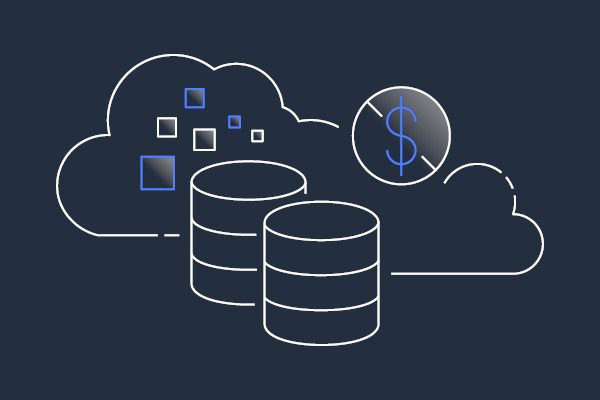
\includegraphics[scale = 0.70]{figs/db-logo-dollar}};","","  \\draw[comm] (t-alice) -- (t-alice |- isolation.north);","  \\draw[comm] (t-bob) -- (t-bob |- isolation.north);","  \\draw[comm] (t-carol) -- (t-carol |- isolation.north);","  \\draw[comm] (isolation) -- (isolation |- db.north);","","  \\node[txn, below = 0.50cm of db, fill = green!30] (t-bob-execution)","    {$\\readevent(\\acctone, -40)$ \\\\[2pt]","     $\\readevent(\\accttwo, 60)$};","","  \\node[txn, left = of t-bob-execution] (t-alice-execution)","    {$\\readevent(\\acctone, 60)$ \\\\[2pt]","     $\\readevent(\\accttwo, 60)$ \\\\[2pt]","     $\\writeevent(\\acctone, -40)$};","","  \\node[txn, right = of t-bob-execution] (t-carol-execution)","    {$\\readevent(\\acctone, -40)$ \\\\[2pt]","     $\\readevent(\\accttwo, 60)$};","\\end{tikzpicture}"],"stylingDirectives":null,"colorizedLines":["\u003cspan class=\"pl-c\"\u003e\u003cspan class=\"pl-c\"\u003e%\u003c/span\u003e isolation-ser-write-skew-tikz.tex\u003c/span\u003e","","\u003cspan class=\"pl-c1\"\u003e\\begin\u003c/span\u003e{\u003cspan class=\"pl-smi\"\u003etikzpicture\u003c/span\u003e}[","  node distance = 1.5cm and 1.5cm,","  txn/.style = {draw, inner sep = 3pt, align = center},","  comm/.style = {arrows = {Stealth-Stealth}, ultra thick, purple}]","","  \u003cspan class=\"pl-c1\"\u003e\\node\u003c/span\u003e[txn] (t-alice)","    {\u003cspan class=\"pl-s\"\u003e\u003cspan class=\"pl-pds\"\u003e$\u003c/span\u003ex_{1} \u003cspan class=\"pl-c1\"\u003e\\gets\u003c/span\u003e \u003cspan class=\"pl-c1\"\u003e\\readevent\u003c/span\u003e(\u003cspan class=\"pl-c1\"\u003e\\acctone\u003c/span\u003e)\u003cspan class=\"pl-pds\"\u003e$\u003c/span\u003e\u003c/span\u003e\u003cspan class=\"pl-c1\"\u003e\\\\\u003c/span\u003e[2pt]","     \u003cspan class=\"pl-s\"\u003e\u003cspan class=\"pl-pds\"\u003e$\u003c/span\u003ex_{2} \u003cspan class=\"pl-c1\"\u003e\\gets\u003c/span\u003e \u003cspan class=\"pl-c1\"\u003e\\readevent\u003c/span\u003e(\u003cspan class=\"pl-c1\"\u003e\\accttwo\u003c/span\u003e)\u003cspan class=\"pl-pds\"\u003e$\u003c/span\u003e\u003c/span\u003e\u003cspan class=\"pl-c1\"\u003e\\\\\u003c/span\u003e[2pt]","     \u003cspan class=\"pl-s\"\u003e\u003cspan class=\"pl-pds\"\u003e$\u003c/span\u003e\u003cspan class=\"pl-c1\"\u003e\\text\u003c/span\u003e{\u003cspan class=\"pl-c1\"\u003e\\bf\u003c/span\u003e if}\u003cspan class=\"pl-cce\"\u003e\\;\u003c/span\u003e x_{1} + x_{2} \u0026gt; \u003cspan class=\"pl-c1\"\u003e100\u003c/span\u003e\u003cspan class=\"pl-pds\"\u003e$\u003c/span\u003e\u003c/span\u003e \u003cspan class=\"pl-c1\"\u003e\\\\\u003c/span\u003e[2pt]","     \u003cspan class=\"pl-s\"\u003e\u003cspan class=\"pl-pds\"\u003e$\u003c/span\u003e\u003cspan class=\"pl-c1\"\u003e\\quad\u003c/span\u003e \u003cspan class=\"pl-c1\"\u003e\\red\u003c/span\u003e{x_{1} \u003cspan class=\"pl-c1\"\u003e\\gets\u003c/span\u003e x_{1} - 100}\u003cspan class=\"pl-pds\"\u003e$\u003c/span\u003e\u003c/span\u003e \u003cspan class=\"pl-c1\"\u003e\\\\\u003c/span\u003e[2pt]","     \u003cspan class=\"pl-s\"\u003e\u003cspan class=\"pl-pds\"\u003e$\u003c/span\u003e\u003cspan class=\"pl-c1\"\u003e\\quad\u003c/span\u003e \u003cspan class=\"pl-c1\"\u003e\\writeevent\u003c/span\u003e(\u003cspan class=\"pl-c1\"\u003e\\acctone\u003c/span\u003e, x_{1})\u003cspan class=\"pl-pds\"\u003e$\u003c/span\u003e\u003c/span\u003e};","","  \u003cspan class=\"pl-c1\"\u003e\\node\u003c/span\u003e[txn, right = of t-alice] (t-bob)","    {\u003cspan class=\"pl-s\"\u003e\u003cspan class=\"pl-pds\"\u003e$\u003c/span\u003ex_{1} \u003cspan class=\"pl-c1\"\u003e\\gets\u003c/span\u003e \u003cspan class=\"pl-c1\"\u003e\\readevent\u003c/span\u003e(\u003cspan class=\"pl-c1\"\u003e\\acctone\u003c/span\u003e)\u003cspan class=\"pl-pds\"\u003e$\u003c/span\u003e\u003c/span\u003e\u003cspan class=\"pl-c1\"\u003e\\\\\u003c/span\u003e[2pt]","     \u003cspan class=\"pl-s\"\u003e\u003cspan class=\"pl-pds\"\u003e$\u003c/span\u003ex_{2} \u003cspan class=\"pl-c1\"\u003e\\gets\u003c/span\u003e \u003cspan class=\"pl-c1\"\u003e\\readevent\u003c/span\u003e(\u003cspan class=\"pl-c1\"\u003e\\accttwo\u003c/span\u003e)\u003cspan class=\"pl-pds\"\u003e$\u003c/span\u003e\u003c/span\u003e\u003cspan class=\"pl-c1\"\u003e\\\\\u003c/span\u003e[2pt]","     \u003cspan class=\"pl-s\"\u003e\u003cspan class=\"pl-pds\"\u003e$\u003c/span\u003e\u003cspan class=\"pl-c1\"\u003e\\text\u003c/span\u003e{\u003cspan class=\"pl-c1\"\u003e\\bf\u003c/span\u003e if}\u003cspan class=\"pl-cce\"\u003e\\;\u003c/span\u003e x_{1} + x_{2} \u0026gt; \u003cspan class=\"pl-c1\"\u003e100\u003c/span\u003e\u003cspan class=\"pl-pds\"\u003e$\u003c/span\u003e\u003c/span\u003e \u003cspan class=\"pl-c1\"\u003e\\\\\u003c/span\u003e[2pt]","     \u003cspan class=\"pl-s\"\u003e\u003cspan class=\"pl-pds\"\u003e$\u003c/span\u003e\u003cspan class=\"pl-c1\"\u003e\\quad\u003c/span\u003e \u003cspan class=\"pl-c1\"\u003e\\red\u003c/span\u003e{x_{2} \u003cspan class=\"pl-c1\"\u003e\\gets\u003c/span\u003e x_{2} - 100}\u003cspan class=\"pl-pds\"\u003e$\u003c/span\u003e\u003c/span\u003e \u003cspan class=\"pl-c1\"\u003e\\\\\u003c/span\u003e[2pt]","     \u003cspan class=\"pl-s\"\u003e\u003cspan class=\"pl-pds\"\u003e$\u003c/span\u003e\u003cspan class=\"pl-c1\"\u003e\\quad\u003c/span\u003e \u003cspan class=\"pl-c1\"\u003e\\writeevent\u003c/span\u003e(\u003cspan class=\"pl-c1\"\u003e\\accttwo\u003c/span\u003e, x_{2})\u003cspan class=\"pl-pds\"\u003e$\u003c/span\u003e\u003c/span\u003e};","","  \u003cspan class=\"pl-c1\"\u003e\\node\u003c/span\u003e[txn, right = of t-bob] (t-carol)","    {\u003cspan class=\"pl-s\"\u003e\u003cspan class=\"pl-pds\"\u003e$\u003c/span\u003ex_{1} \u003cspan class=\"pl-c1\"\u003e\\gets\u003c/span\u003e \u003cspan class=\"pl-c1\"\u003e\\readevent\u003c/span\u003e(\u003cspan class=\"pl-c1\"\u003e\\acctone\u003c/span\u003e)\u003cspan class=\"pl-pds\"\u003e$\u003c/span\u003e\u003c/span\u003e\u003cspan class=\"pl-c1\"\u003e\\\\\u003c/span\u003e[2pt]","     \u003cspan class=\"pl-s\"\u003e\u003cspan class=\"pl-pds\"\u003e$\u003c/span\u003ex_{2} \u003cspan class=\"pl-c1\"\u003e\\gets\u003c/span\u003e \u003cspan class=\"pl-c1\"\u003e\\readevent\u003c/span\u003e(\u003cspan class=\"pl-c1\"\u003e\\accttwo\u003c/span\u003e)\u003cspan class=\"pl-pds\"\u003e$\u003c/span\u003e\u003c/span\u003e};","","  \u003cspan class=\"pl-c1\"\u003e\\node\u003c/span\u003e[draw, fill = yellow!50, below = of t-bob, font = \u003cspan class=\"pl-c1\"\u003e\\large\u003c/span\u003e,","    inner sep = 8pt, minimum width = 260pt] (isolation)","    {{Serializability (SER)}};","","  \u003cspan class=\"pl-c1\"\u003e\\node\u003c/span\u003e[below = of isolation,","    label = {[label distance = 5pt]above : {\u003cspan class=\"pl-c1\"\u003e\\large\u003c/span\u003e \u003cspan class=\"pl-s\"\u003e\u003cspan class=\"pl-pds\"\u003e$\u003c/span\u003e\u003cspan class=\"pl-c1\"\u003e\\acctone\u003c/span\u003e = \u003cspan class=\"pl-c1\"\u003e\\accttwo\u003c/span\u003e = \u003cspan class=\"pl-c1\"\u003e60\u003c/span\u003e\u003cspan class=\"pl-pds\"\u003e$\u003c/span\u003e\u003c/span\u003e}}] (db)","    {\u003cspan class=\"pl-c1\"\u003e\\includegraphics\u003c/span\u003e[scale = 0.70]{figs/db-logo-dollar}};","","  \u003cspan class=\"pl-c1\"\u003e\\draw\u003c/span\u003e[comm] (t-alice) -- (t-alice |- isolation.north);","  \u003cspan class=\"pl-c1\"\u003e\\draw\u003c/span\u003e[comm] (t-bob) -- (t-bob |- isolation.north);","  \u003cspan class=\"pl-c1\"\u003e\\draw\u003c/span\u003e[comm] (t-carol) -- (t-carol |- isolation.north);","  \u003cspan class=\"pl-c1\"\u003e\\draw\u003c/span\u003e[comm] (isolation) -- (isolation |- db.north);","","  \u003cspan class=\"pl-c1\"\u003e\\node\u003c/span\u003e[txn, below = 0.50cm of db, fill = green!30] (t-bob-execution)","    {\u003cspan class=\"pl-s\"\u003e\u003cspan class=\"pl-pds\"\u003e$\u003c/span\u003e\u003cspan class=\"pl-c1\"\u003e\\readevent\u003c/span\u003e(\u003cspan class=\"pl-c1\"\u003e\\acctone\u003c/span\u003e, -\u003cspan class=\"pl-c1\"\u003e40\u003c/span\u003e)\u003cspan class=\"pl-pds\"\u003e$\u003c/span\u003e\u003c/span\u003e \u003cspan class=\"pl-c1\"\u003e\\\\\u003c/span\u003e[2pt]","     \u003cspan class=\"pl-s\"\u003e\u003cspan class=\"pl-pds\"\u003e$\u003c/span\u003e\u003cspan class=\"pl-c1\"\u003e\\readevent\u003c/span\u003e(\u003cspan class=\"pl-c1\"\u003e\\accttwo\u003c/span\u003e, \u003cspan class=\"pl-c1\"\u003e60\u003c/span\u003e)\u003cspan class=\"pl-pds\"\u003e$\u003c/span\u003e\u003c/span\u003e};","","  \u003cspan class=\"pl-c1\"\u003e\\node\u003c/span\u003e[txn, left = of t-bob-execution] (t-alice-execution)","    {\u003cspan class=\"pl-s\"\u003e\u003cspan class=\"pl-pds\"\u003e$\u003c/span\u003e\u003cspan class=\"pl-c1\"\u003e\\readevent\u003c/span\u003e(\u003cspan class=\"pl-c1\"\u003e\\acctone\u003c/span\u003e, \u003cspan class=\"pl-c1\"\u003e60\u003c/span\u003e)\u003cspan class=\"pl-pds\"\u003e$\u003c/span\u003e\u003c/span\u003e \u003cspan class=\"pl-c1\"\u003e\\\\\u003c/span\u003e[2pt]","     \u003cspan class=\"pl-s\"\u003e\u003cspan class=\"pl-pds\"\u003e$\u003c/span\u003e\u003cspan class=\"pl-c1\"\u003e\\readevent\u003c/span\u003e(\u003cspan class=\"pl-c1\"\u003e\\accttwo\u003c/span\u003e, \u003cspan class=\"pl-c1\"\u003e60\u003c/span\u003e)\u003cspan class=\"pl-pds\"\u003e$\u003c/span\u003e\u003c/span\u003e \u003cspan class=\"pl-c1\"\u003e\\\\\u003c/span\u003e[2pt]","     \u003cspan class=\"pl-s\"\u003e\u003cspan class=\"pl-pds\"\u003e$\u003c/span\u003e\u003cspan class=\"pl-c1\"\u003e\\writeevent\u003c/span\u003e(\u003cspan class=\"pl-c1\"\u003e\\acctone\u003c/span\u003e, -\u003cspan class=\"pl-c1\"\u003e40\u003c/span\u003e)\u003cspan class=\"pl-pds\"\u003e$\u003c/span\u003e\u003c/span\u003e};","","  \u003cspan class=\"pl-c1\"\u003e\\node\u003c/span\u003e[txn, right = of t-bob-execution] (t-carol-execution)","    {\u003cspan class=\"pl-s\"\u003e\u003cspan class=\"pl-pds\"\u003e$\u003c/span\u003e\u003cspan class=\"pl-c1\"\u003e\\readevent\u003c/span\u003e(\u003cspan class=\"pl-c1\"\u003e\\acctone\u003c/span\u003e, -\u003cspan class=\"pl-c1\"\u003e40\u003c/span\u003e)\u003cspan class=\"pl-pds\"\u003e$\u003c/span\u003e\u003c/span\u003e \u003cspan class=\"pl-c1\"\u003e\\\\\u003c/span\u003e[2pt]","     \u003cspan class=\"pl-s\"\u003e\u003cspan class=\"pl-pds\"\u003e$\u003c/span\u003e\u003cspan class=\"pl-c1\"\u003e\\readevent\u003c/span\u003e(\u003cspan class=\"pl-c1\"\u003e\\accttwo\u003c/span\u003e, \u003cspan class=\"pl-c1\"\u003e60\u003c/span\u003e)\u003cspan class=\"pl-pds\"\u003e$\u003c/span\u003e\u003c/span\u003e};","\u003cspan class=\"pl-c1\"\u003e\\end\u003c/span\u003e{\u003cspan class=\"pl-smi\"\u003etikzpicture\u003c/span\u003e}"],"csv":null,"csvError":null,"copilotSWEAgentEnabled":true,"dependabotInfo":{"showConfigurationBanner":false,"configFilePath":null,"networkDependabotPath":"/reports-by-hfwei/polysi-vldb2023-report/network/updates","dismissConfigurationNoticePath":"/settings/dismiss-notice/dependabot_configuration_notice","configurationNoticeDismissed":false},"displayName":"isolation-ser-write-skew-tikz.tex","displayUrl":"https://github.com/reports-by-hfwei/polysi-vldb2023-report/blob/main/tikz/isolation-ser-write-skew-tikz.tex?raw=true","headerInfo":{"blobSize":"1.88 KB","deleteTooltip":"Delete this file","editTooltip":"Edit this file","ghDesktopPath":"https://desktop.github.com","isGitLfs":false,"onBranch":true,"shortPath":"9f66ded","siteNavLoginPath":"/login?return_to=https%3A%2F%2Fgithub.com%2Freports-by-hfwei%2Fpolysi-vldb2023-report%2Fblob%2Fmain%2Ftikz%2Fisolation-ser-write-skew-tikz.tex","isCSV":false,"isRichtext":false,"toc":null,"lineInfo":{"truncatedLoc":"51","truncatedSloc":"41"},"mode":"file"},"image":false,"isCodeownersFile":null,"isPlain":false,"isValidLegacyIssueTemplate":false,"issueTemplate":null,"discussionTemplate":null,"language":"TeX","languageID":369,"large":false,"planSupportInfo":{"repoIsFork":null,"repoOwnedByCurrentUser":null,"requestFullPath":"/reports-by-hfwei/polysi-vldb2023-report/blob/main/tikz/isolation-ser-write-skew-tikz.tex","showFreeOrgGatedFeatureMessage":null,"showPlanSupportBanner":null,"upgradeDataAttributes":null,"upgradePath":null},"publishBannersInfo":{"dismissActionNoticePath":"/settings/dismiss-notice/publish_action_from_dockerfile","releasePath":"/reports-by-hfwei/polysi-vldb2023-report/releases/new?marketplace=true","showPublishActionBanner":false},"rawBlobUrl":"https://github.com/reports-by-hfwei/polysi-vldb2023-report/raw/refs/heads/main/tikz/isolation-ser-write-skew-tikz.tex","renderImageOrRaw":false,"richText":null,"renderedFileInfo":null,"shortPath":null,"symbolsEnabled":true,"tabSize":4,"topBannersInfo":{"overridingGlobalFundingFile":false,"globalPreferredFundingPath":null,"showInvalidCitationWarning":false,"citationHelpUrl":"https://docs.github.com/github/creating-cloning-and-archiving-repositories/creating-a-repository-on-github/about-citation-files","actionsOnboardingTip":null},"truncated":false,"viewable":true,"workflowRedirectUrl":null,"symbols":{"timed_out":false,"not_analyzed":true,"symbols":[]}},"copilotInfo":null,"copilotAccessAllowed":true,"modelsAccessAllowed":false,"modelsRepoIntegrationEnabled":false,"isMarketplaceEnabled":true,"csrf_tokens":{"/reports-by-hfwei/polysi-vldb2023-report/branches":{"post":"GqWUmaEU4R8FMOJNaDieP_V11JeQjfeWa59MzeYK8FOlsCek03RIXs4RvFcVfh5nqYyIpYs4fbTsRItktfbkAA"},"/repos/preferences":{"post":"V-TZsTBdZxaJZq68wEIATOqs46q1ugFqnCvVo4bnxhDiMNlJXi8luW6zuK3pC1Hw7WnwZ43b9wACsFdP-U2vuQ"}}},"title":"polysi-vldb2023-report/tikz/isolation-ser-write-skew-tikz.tex at main · reports-by-hfwei/polysi-vldb2023-report","appPayload":{"helpUrl":"https://docs.github.com","findFileWorkerPath":"/assets-cdn/worker/find-file-worker-9bd411a8e273.js","findInFileWorkerPath":"/assets-cdn/worker/find-in-file-worker-410714137fc9.js","githubDevUrl":"https://github.dev/","enabled_features":{"code_nav_ui_events":false,"react_blob_overlay":true,"accessible_code_button":true}}}</script>
  <div data-target="react-app.reactRoot"><style data-styled="true" data-styled-version="5.3.11">.gISSDQ{width:100%;}/*!sc*/
@media screen and (min-width:544px){.gISSDQ{width:100%;}}/*!sc*/
@media screen and (min-width:768px){.gISSDQ{width:auto;}}/*!sc*/
.birIjn{max-height:100%;height:100%;display:-webkit-box;display:-webkit-flex;display:-ms-flexbox;display:flex;-webkit-flex-direction:column;-ms-flex-direction:column;flex-direction:column;}/*!sc*/
@media screen and (max-width:768px){.birIjn{display:none;}}/*!sc*/
@media screen and (min-width:768px){.birIjn{max-height:100vh;height:100vh;}}/*!sc*/
.jfIeyl{display:-webkit-box;display:-webkit-flex;display:-ms-flexbox;display:flex;width:100%;margin-bottom:16px;-webkit-align-items:center;-webkit-box-align:center;-ms-flex-align:center;align-items:center;}/*!sc*/
.kOkWgo{font-size:16px;margin-left:8px;}/*!sc*/
.dPUXSa[data-size="medium"][data-no-visuals]{border-top-left-radius:0;border-bottom-left-radius:0;}/*!sc*/
@media screen and (max-width:768px){.jLLPHh{display:none;}}/*!sc*/
.bHLmSv{position:absolute;inset:0 -2px;cursor:col-resize;background-color:transparent;-webkit-transition-delay:0.1s;transition-delay:0.1s;}/*!sc*/
.bHLmSv:hover{background-color:var(--bgColor-neutral-muted,var(--color-neutral-muted,rgba(175,184,193,0.2)));}/*!sc*/
.leYMvG{margin-left:auto;margin-right:auto;-webkit-flex-direction:column;-ms-flex-direction:column;flex-direction:column;padding-bottom:40px;max-width:100%;margin-top:0;}/*!sc*/
.KMPzq{display:inherit;}/*!sc*/
.cEytCf{display:-webkit-box;display:-webkit-flex;display:-ms-flexbox;display:flex;-webkit-flex-direction:row;-ms-flex-direction:row;flex-direction:row;font-size:16px;min-width:0;-webkit-flex-shrink:1;-ms-flex-negative:1;flex-shrink:1;-webkit-flex-wrap:wrap;-ms-flex-wrap:wrap;flex-wrap:wrap;max-width:100%;-webkit-align-items:center;-webkit-box-align:center;-ms-flex-align:center;align-items:center;}/*!sc*/
.fzFXnm{max-width:100%;}/*!sc*/
.iMnkmv{max-width:100%;list-style:none;display:inline-block;}/*!sc*/
.ghzDag{display:inline-block;max-width:100%;}/*!sc*/
.kHuKdh{font-weight:600;}/*!sc*/
.hzJBof{padding-left:4px;padding-right:4px;font-weight:400;color:var(--fgColor-muted,var(--color-fg-muted,#656d76));font-size:16px;}/*!sc*/
.kgiVEz{font-weight:400;}/*!sc*/
.jGhzSQ{font-weight:600;display:inline-block;max-width:100%;font-size:16px;}/*!sc*/
.fjrFuv[data-size="medium"][data-no-visuals]{display:none;}/*!sc*/
.gUkoLg{-webkit-box-pack:center;-webkit-justify-content:center;-ms-flex-pack:center;justify-content:center;}/*!sc*/
.dJxjrT{margin-left:16px;margin-right:16px;}/*!sc*/
.ldRxiI{display:-webkit-box;display:-webkit-flex;display:-ms-flexbox;display:flex;-webkit-flex-direction:row;-ms-flex-direction:row;flex-direction:row;}/*!sc*/
.fVkfyA{width:100%;height:-webkit-fit-content;height:-moz-fit-content;height:fit-content;min-width:0;margin-right:0;}/*!sc*/
.gNAmSV{height:40px;padding-left:4px;padding-bottom:16px;}/*!sc*/
.jdLMhu{top:0px;z-index:4;background:var(--bgColor-default,var(--color-canvas-default));position:-webkit-sticky;position:sticky;}/*!sc*/
.hqwSEx{display:none;min-width:0;padding-top:8px;padding-bottom:8px;}/*!sc*/
.fHind{display:-webkit-box;display:-webkit-flex;display:-ms-flexbox;display:flex;-webkit-flex-direction:row;-ms-flex-direction:row;flex-direction:row;font-size:14px;min-width:0;-webkit-flex-shrink:1;-ms-flex-negative:1;flex-shrink:1;-webkit-flex-wrap:wrap;-ms-flex-wrap:wrap;flex-wrap:wrap;max-width:100%;-webkit-align-items:center;-webkit-box-align:center;-ms-flex-align:center;align-items:center;}/*!sc*/
.oDtgN{padding-left:4px;padding-right:4px;font-weight:400;color:var(--fgColor-muted,var(--color-fg-muted,#656d76));font-size:14px;}/*!sc*/
.dnZoUW{font-weight:600;display:inline-block;max-width:100%;font-size:14px;}/*!sc*/
.gFKFyc{border-radius:6px 6px 0px 0px;}/*!sc*/
.lefpaC linkButtonSx:hover:not([disabled]){-webkit-text-decoration:none;text-decoration:none;}/*!sc*/
.lefpaC linkButtonSx:focus:not([disabled]){-webkit-text-decoration:none;text-decoration:none;}/*!sc*/
.lefpaC linkButtonSx:active:not([disabled]){-webkit-text-decoration:none;text-decoration:none;}/*!sc*/
.ivobqY[data-size="small"][data-no-visuals]{border-top-left-radius:0;border-bottom-left-radius:0;}/*!sc*/
.iCOsHh[data-size="small"][data-no-visuals]:hover:not([disabled]){-webkit-text-decoration:none;text-decoration:none;}/*!sc*/
.iCOsHh[data-size="small"][data-no-visuals]:focus:not([disabled]){-webkit-text-decoration:none;text-decoration:none;}/*!sc*/
.iCOsHh[data-size="small"][data-no-visuals]:active:not([disabled]){-webkit-text-decoration:none;text-decoration:none;}/*!sc*/
.hGyMdv{border:1px solid;border-top:none;border-color:var(--borderColor-default,var(--color-border-default,#d0d7de));border-radius:0px 0px 6px 6px;min-width:273px;}/*!sc*/
.dceWRL{background-color:var(--bgColor-default,var(--color-canvas-default));border:0px;border-width:0;border-radius:0px 0px 6px 6px;padding:0;min-width:0;margin-top:46px;}/*!sc*/
.dGXHv{display:-webkit-box;display:-webkit-flex;display:-ms-flexbox;display:flex;-webkit-flex:1;-ms-flex:1;flex:1;padding-top:8px;padding-bottom:8px;-webkit-flex-direction:column;-ms-flex-direction:column;flex-direction:column;-webkit-box-pack:justify;-webkit-justify-content:space-between;-ms-flex-pack:justify;justify-content:space-between;min-width:0;position:relative;}/*!sc*/
.bpDFns{position:relative;}/*!sc*/
.iJOeCH{-webkit-flex:1;-ms-flex:1;flex:1;position:relative;min-width:0;}/*!sc*/
.glDApP{tab-size:4;isolation:isolate;position:relative;overflow:auto;max-width:unset;}/*!sc*/
.cCoXib{position:fixed;top:0;right:0;height:100%;width:15px;-webkit-transition:-webkit-transform 0.3s;-webkit-transition:transform 0.3s;transition:transform 0.3s;z-index:1;}/*!sc*/
.cCoXib:hover{-webkit-transform:scaleX(1.5);-ms-transform:scaleX(1.5);transform:scaleX(1.5);}/*!sc*/
data-styled.g1[id="Box-sc-g0xbh4-0"]{content:"gISSDQ,birIjn,jfIeyl,kOkWgo,dPUXSa,jLLPHh,bHLmSv,leYMvG,KMPzq,cEytCf,fzFXnm,iMnkmv,ghzDag,kHuKdh,hzJBof,kgiVEz,jGhzSQ,fjrFuv,gUkoLg,dJxjrT,ldRxiI,fVkfyA,gNAmSV,jdLMhu,hqwSEx,fHind,oDtgN,dnZoUW,gFKFyc,lefpaC,ivobqY,iCOsHh,hGyMdv,dceWRL,dGXHv,bpDFns,iJOeCH,glDApP,cCoXib,"}/*!sc*/
.hWlpPn{position:relative;display:inline-block;}/*!sc*/
.hWlpPn::after{position:absolute;z-index:1000000;display:none;padding:0.5em 0.75em;font:normal normal 11px/1.5 -apple-system,BlinkMacSystemFont,"Segoe UI","Noto Sans",Helvetica,Arial,sans-serif,"Apple Color Emoji","Segoe UI Emoji";-webkit-font-smoothing:subpixel-antialiased;color:var(--tooltip-fgColor,var(--fgColor-onEmphasis,var(--color-fg-on-emphasis,#ffffff)));text-align:center;-webkit-text-decoration:none;text-decoration:none;text-shadow:none;text-transform:none;-webkit-letter-spacing:normal;-moz-letter-spacing:normal;-ms-letter-spacing:normal;letter-spacing:normal;word-wrap:break-word;white-space:pre;pointer-events:none;content:attr(aria-label);background:var(--tooltip-bgColor,var(--bgColor-emphasis,var(--color-neutral-emphasis-plus,#24292f)));border-radius:6px;opacity:0;}/*!sc*/
@-webkit-keyframes tooltip-appear{from{opacity:0;}to{opacity:1;}}/*!sc*/
@keyframes tooltip-appear{from{opacity:0;}to{opacity:1;}}/*!sc*/
.hWlpPn:hover::after,.hWlpPn:active::after,.hWlpPn:focus::after,.hWlpPn:focus-within::after{display:inline-block;-webkit-text-decoration:none;text-decoration:none;-webkit-animation-name:tooltip-appear;animation-name:tooltip-appear;-webkit-animation-duration:0.1s;animation-duration:0.1s;-webkit-animation-fill-mode:forwards;animation-fill-mode:forwards;-webkit-animation-timing-function:ease-in;animation-timing-function:ease-in;-webkit-animation-delay:0s;animation-delay:0s;}/*!sc*/
.hWlpPn.tooltipped-no-delay:hover::after,.hWlpPn.tooltipped-no-delay:active::after,.hWlpPn.tooltipped-no-delay:focus::after,.hWlpPn.tooltipped-no-delay:focus-within::after{-webkit-animation-delay:0s;animation-delay:0s;}/*!sc*/
.hWlpPn.tooltipped-multiline:hover::after,.hWlpPn.tooltipped-multiline:active::after,.hWlpPn.tooltipped-multiline:focus::after,.hWlpPn.tooltipped-multiline:focus-within::after{display:table-cell;}/*!sc*/
.hWlpPn.tooltipped-s::after,.hWlpPn.tooltipped-se::after,.hWlpPn.tooltipped-sw::after{top:100%;right:50%;margin-top:6px;}/*!sc*/
.hWlpPn.tooltipped-se::after{right:auto;left:50%;margin-left:-16px;}/*!sc*/
.hWlpPn.tooltipped-sw::after{margin-right:-16px;}/*!sc*/
.hWlpPn.tooltipped-n::after,.hWlpPn.tooltipped-ne::after,.hWlpPn.tooltipped-nw::after{right:50%;bottom:100%;margin-bottom:6px;}/*!sc*/
.hWlpPn.tooltipped-ne::after{right:auto;left:50%;margin-left:-16px;}/*!sc*/
.hWlpPn.tooltipped-nw::after{margin-right:-16px;}/*!sc*/
.hWlpPn.tooltipped-s::after,.hWlpPn.tooltipped-n::after{-webkit-transform:translateX(50%);-ms-transform:translateX(50%);transform:translateX(50%);}/*!sc*/
.hWlpPn.tooltipped-w::after{right:100%;bottom:50%;margin-right:6px;-webkit-transform:translateY(50%);-ms-transform:translateY(50%);transform:translateY(50%);}/*!sc*/
.hWlpPn.tooltipped-e::after{bottom:50%;left:100%;margin-left:6px;-webkit-transform:translateY(50%);-ms-transform:translateY(50%);transform:translateY(50%);}/*!sc*/
.hWlpPn.tooltipped-multiline::after{width:-webkit-max-content;width:-moz-max-content;width:max-content;max-width:250px;word-wrap:break-word;white-space:pre-line;border-collapse:separate;}/*!sc*/
.hWlpPn.tooltipped-multiline.tooltipped-s::after,.hWlpPn.tooltipped-multiline.tooltipped-n::after{right:auto;left:50%;-webkit-transform:translateX(-50%);-ms-transform:translateX(-50%);transform:translateX(-50%);}/*!sc*/
.hWlpPn.tooltipped-multiline.tooltipped-w::after,.hWlpPn.tooltipped-multiline.tooltipped-e::after{right:100%;}/*!sc*/
.hWlpPn.tooltipped-align-right-2::after{right:0;margin-right:0;}/*!sc*/
.hWlpPn.tooltipped-align-left-2::after{left:0;margin-left:0;}/*!sc*/
data-styled.g4[id="Tooltip__TooltipBase-sc-17tf59c-0"]{content:"hWlpPn,"}/*!sc*/
</style><meta data-hydrostats="publish"/> <!-- --> <!-- --> <button hidden="" data-testid="header-permalink-button" data-hotkey-scope="read-only-cursor-text-area"></button><button hidden=""></button><div><div style="--spacing:var(--spacing-none)" class="prc-PageLayout-PageLayoutRoot-1zlEO"><div class="prc-PageLayout-PageLayoutWrapper-s2ao4" data-width="full"><div class="prc-PageLayout-PageLayoutContent-jzDMn"><div tabindex="0" class="Box-sc-g0xbh4-0 gISSDQ"><div class="prc-PageLayout-PaneWrapper-nGO0U ReposFileTreePane-module__Pane--D26Sw ReposFileTreePane-module__HidePaneWithTreeOverlay--CJn2n" style="--offset-header:0px;--spacing-row:var(--spacing-none);--spacing-column:var(--spacing-none)" data-is-hidden="false" data-position="start" data-sticky="true"><div class="prc-PageLayout-HorizontalDivider-CYLp5 prc-PageLayout-PaneHorizontalDivider-4exOb" data-variant="none" data-position="start" style="--spacing-divider:var(--spacing-none);--spacing:var(--spacing-none)"></div><div class="prc-PageLayout-Pane-Vl5LI" data-resizable="true" style="--spacing:var(--spacing-none);--pane-min-width:256px;--pane-max-width:calc(100vw - var(--pane-max-width-diff));--pane-width-size:var(--pane-width-large);--pane-width:320px"><div class="react-tree-pane-contents-3-panel"><div id="repos-file-tree" class="Box-sc-g0xbh4-0 birIjn"><div class="ReposFileTreePane-module__Box_1--ZT_4S"><div class="Box-sc-g0xbh4-0 jfIeyl"><h2 class="use-tree-pane-module__Heading--iI_ad prc-Heading-Heading-6CmGO"><button type="button" aria-label="Expand file tree" data-testid="expand-file-tree-button-mobile" class="prc-Button-ButtonBase-c50BI ExpandFileTreeButton-module__Button_1--g8F6Q" data-loading="false" data-size="medium" data-variant="invisible" aria-describedby=":Rl6mplab:-loading-announcement"><span data-component="buttonContent" data-align="center" class="prc-Button-ButtonContent-HKbr-"><span data-component="leadingVisual" class="prc-Button-Visual-2epfX prc-Button-VisualWrap-Db-eB"><svg aria-hidden="true" focusable="false" class="octicon octicon-arrow-left" viewBox="0 0 16 16" width="16" height="16" fill="currentColor" display="inline-block" overflow="visible" style="vertical-align:text-bottom"><path d="M7.78 12.53a.75.75 0 0 1-1.06 0L2.47 8.28a.75.75 0 0 1 0-1.06l4.25-4.25a.751.751 0 0 1 1.042.018.751.751 0 0 1 .018 1.042L4.81 7h7.44a.75.75 0 0 1 0 1.5H4.81l2.97 2.97a.75.75 0 0 1 0 1.06Z"></path></svg></span><span data-component="text" class="prc-Button-Label-pTQ3x">Files</span></span></button><button data-component="IconButton" type="button" data-testid="collapse-file-tree-button" aria-expanded="true" aria-controls="repos-file-tree" class="prc-Button-ButtonBase-c50BI position-relative ExpandFileTreeButton-module__expandButton--oKI1R ExpandFileTreeButton-module__filesButtonBreakpoint--03FKA fgColor-muted prc-Button-IconButton-szpyj" data-loading="false" data-no-visuals="true" data-size="medium" data-variant="invisible" aria-describedby=":R756mplab:-loading-announcement" aria-labelledby=":R156mplab:"><svg aria-hidden="true" focusable="false" class="octicon octicon-sidebar-expand" viewBox="0 0 16 16" width="16" height="16" fill="currentColor" display="inline-block" overflow="visible" style="vertical-align:text-bottom"><path d="m4.177 7.823 2.396-2.396A.25.25 0 0 1 7 5.604v4.792a.25.25 0 0 1-.427.177L4.177 8.177a.25.25 0 0 1 0-.354Z"></path><path d="M0 1.75C0 .784.784 0 1.75 0h12.5C15.216 0 16 .784 16 1.75v12.5A1.75 1.75 0 0 1 14.25 16H1.75A1.75 1.75 0 0 1 0 14.25Zm1.75-.25a.25.25 0 0 0-.25.25v12.5c0 .138.112.25.25.25H9.5v-13Zm12.5 13a.25.25 0 0 0 .25-.25V1.75a.25.25 0 0 0-.25-.25H11v13Z"></path></svg></button><span class="prc-TooltipV2-Tooltip-cYMVY" data-direction="se" aria-hidden="true" id=":R156mplab:">Collapse file tree</span><button hidden="" data-testid="" data-hotkey-scope="read-only-cursor-text-area"></button></h2><h2 class="Box-sc-g0xbh4-0 kOkWgo prc-Heading-Heading-6CmGO">Files</h2></div><div class="ReposFileTreePane-module__Box_2--RgzGf"><div class="ReposFileTreePane-module__Box_3--XDLn8"><button style="min-width:0" type="button" aria-haspopup="true" aria-expanded="false" tabindex="0" aria-label="main branch" data-testid="anchor-button" class="prc-Button-ButtonBase-c50BI react-repos-tree-pane-ref-selector width-full ref-selector-class RefSelectorAnchoredOverlay-module__RefSelectorOverlayBtn--D34zl" data-loading="false" data-size="medium" data-variant="default" aria-describedby="ref-picker-repos-header-ref-selector-loading-announcement" id="ref-picker-repos-header-ref-selector"><span data-component="buttonContent" data-align="center" class="prc-Button-ButtonContent-HKbr-"><span data-component="text" class="prc-Button-Label-pTQ3x"><div class="RefSelectorAnchoredOverlay-module__RefSelectorOverlayContainer--mCbv8"><div class="RefSelectorAnchoredOverlay-module__RefSelectorOverlayHeader--D4cnZ"><svg aria-hidden="true" focusable="false" class="octicon octicon-git-branch" viewBox="0 0 16 16" width="16" height="16" fill="currentColor" display="inline-block" overflow="visible" style="vertical-align:text-bottom"><path d="M9.5 3.25a2.25 2.25 0 1 1 3 2.122V6A2.5 2.5 0 0 1 10 8.5H6a1 1 0 0 0-1 1v1.128a2.251 2.251 0 1 1-1.5 0V5.372a2.25 2.25 0 1 1 1.5 0v1.836A2.493 2.493 0 0 1 6 7h4a1 1 0 0 0 1-1v-.628A2.25 2.25 0 0 1 9.5 3.25Zm-6 0a.75.75 0 1 0 1.5 0 .75.75 0 0 0-1.5 0Zm8.25-.75a.75.75 0 1 0 0 1.5.75.75 0 0 0 0-1.5ZM4.25 12a.75.75 0 1 0 0 1.5.75.75 0 0 0 0-1.5Z"></path></svg></div><div class="ref-selector-button-text-container RefSelectorAnchoredOverlay-module__RefSelectorBtnTextContainer--yO402"><span class="RefSelectorAnchoredOverlay-module__RefSelectorText--bxVhQ"> <!-- -->main</span></div></div></span><span data-component="trailingVisual" class="prc-Button-Visual-2epfX prc-Button-VisualWrap-Db-eB"><svg aria-hidden="true" focusable="false" class="octicon octicon-triangle-down" viewBox="0 0 16 16" width="16" height="16" fill="currentColor" display="inline-block" overflow="visible" style="vertical-align:text-bottom"><path d="m4.427 7.427 3.396 3.396a.25.25 0 0 0 .354 0l3.396-3.396A.25.25 0 0 0 11.396 7H4.604a.25.25 0 0 0-.177.427Z"></path></svg></span></span></button><button hidden="" data-hotkey-scope="read-only-cursor-text-area"></button></div><div class="ReposFileTreePane-module__Box_4--TLAAU"><a data-component="IconButton" type="button" class="prc-Button-ButtonBase-c50BI ReposFileTreePane-module__IconButton--fpuBk prc-Button-IconButton-szpyj" data-loading="false" data-no-visuals="true" data-size="medium" data-variant="default" aria-describedby=":R6q6mplab:-loading-announcement" aria-labelledby=":Rq6mplab:" href="/reports-by-hfwei/polysi-vldb2023-report/new/main/tikz" data-discover="true"><svg aria-hidden="true" focusable="false" class="octicon octicon-plus" viewBox="0 0 16 16" width="16" height="16" fill="currentColor" display="inline-block" overflow="visible" style="vertical-align:text-bottom"><path d="M7.75 2a.75.75 0 0 1 .75.75V7h4.25a.75.75 0 0 1 0 1.5H8.5v4.25a.75.75 0 0 1-1.5 0V8.5H2.75a.75.75 0 0 1 0-1.5H7V2.75A.75.75 0 0 1 7.75 2Z"></path></svg></a><span class="prc-TooltipV2-Tooltip-cYMVY" data-direction="n" aria-hidden="true" id=":Rq6mplab:">Add file</span><button data-component="IconButton" type="button" class="Box-sc-g0xbh4-0 dPUXSa prc-Button-ButtonBase-c50BI SearchButton-module__IconButton--kxA3Q prc-Button-IconButton-szpyj" data-loading="false" data-no-visuals="true" data-size="medium" data-variant="default" aria-describedby=":Rra6mplab:-loading-announcement" aria-labelledby=":R3a6mplab:"><svg aria-hidden="true" focusable="false" class="octicon octicon-search" viewBox="0 0 16 16" width="16" height="16" fill="currentColor" display="inline-block" overflow="visible" style="vertical-align:text-bottom"><path d="M10.68 11.74a6 6 0 0 1-7.922-8.982 6 6 0 0 1 8.982 7.922l3.04 3.04a.749.749 0 0 1-.326 1.275.749.749 0 0 1-.734-.215ZM11.5 7a4.499 4.499 0 1 0-8.997 0A4.499 4.499 0 0 0 11.5 7Z"></path></svg></button><span class="prc-TooltipV2-Tooltip-cYMVY" data-direction="nw" aria-hidden="true" id=":R3a6mplab:">Search this repository</span><button hidden="" data-testid="" data-hotkey-scope="read-only-cursor-text-area"></button></div></div></div><div class="Box-sc-g0xbh4-0 jLLPHh ReposFileTreePane-module__FileResultsList--YEf_n FileResultsList-module__Box_1--b75fu"><span class="FileResultsList-module__FilesSearchBox--fSAh3 FilesSearchBox-module__TextInput--Rvr17 TextInput-wrapper prc-components-TextInputWrapper-i1ofR prc-components-TextInputBaseWrapper-ueK9q" data-leading-visual="true" data-trailing-visual="true" aria-busy="false"><span class="TextInput-icon" id=":R5amplab:" aria-hidden="true"><svg aria-hidden="true" focusable="false" class="octicon octicon-search" viewBox="0 0 16 16" width="16" height="16" fill="currentColor" display="inline-block" overflow="visible" style="vertical-align:text-bottom"><path d="M10.68 11.74a6 6 0 0 1-7.922-8.982 6 6 0 0 1 8.982 7.922l3.04 3.04a.749.749 0 0 1-.326 1.275.749.749 0 0 1-.734-.215ZM11.5 7a4.499 4.499 0 1 0-8.997 0A4.499 4.499 0 0 0 11.5 7Z"></path></svg></span><input type="text" aria-label="Go to file" role="combobox" aria-controls="file-results-list" aria-expanded="false" aria-haspopup="dialog" autoCorrect="off" spellcheck="false" placeholder="Go to file" aria-describedby=":R5amplab: :R5amplabH1:" data-component="input" class="prc-components-Input-Ic-y8" value=""/><span class="TextInput-icon" id=":R5amplabH1:" aria-hidden="true"><div class="FilesSearchBox-module__Box--QJMeO"><kbd>t</kbd></div></span></span></div><button hidden="" data-testid="" data-hotkey-scope="read-only-cursor-text-area"></button><button hidden=""></button><div class="Box-sc-g0xbh4-0 jLLPHh ReposFileTreePane-module__Box_5--cckih"><div class="react-tree-show-tree-items"><div class="ReposFileTreeView-module__Box--bDodO" data-testid="repos-file-tree-container"><nav aria-label="File Tree Navigation"><span class="prc-src-InternalVisuallyHidden-nlR9R" role="status" aria-live="polite" aria-atomic="true"></span><ul role="tree" aria-label="Files" data-truncate-text="true" class="prc-TreeView-TreeViewRootUlStyles-eZtxW"><li class="PRIVATE_TreeView-item prc-TreeView-TreeViewItem-ShJr0" tabindex="0" id="figs-item" role="treeitem" aria-labelledby=":R3pimplab:" aria-describedby=":R3pimplabH1:" aria-level="1" aria-expanded="false" aria-selected="false"><div class="PRIVATE_TreeView-item-container prc-TreeView-TreeViewItemContainer--2Rkn" style="--level:1;content-visibility:auto;contain-intrinsic-size:auto 2rem"><div style="grid-area:spacer;display:flex"><div style="width:100%;display:flex"></div></div><div class="PRIVATE_TreeView-item-toggle PRIVATE_TreeView-item-toggle--hover PRIVATE_TreeView-item-toggle--end prc-TreeView-TreeViewItemToggle-gWUdE prc-TreeView-TreeViewItemToggleHover-nEgP- prc-TreeView-TreeViewItemToggleEnd-t-AEB"><svg aria-hidden="true" focusable="false" class="octicon octicon-chevron-right" viewBox="0 0 12 12" width="12" height="12" fill="currentColor" display="inline-block" overflow="visible" style="vertical-align:text-bottom"><path d="M4.7 10c-.2 0-.4-.1-.5-.2-.3-.3-.3-.8 0-1.1L6.9 6 4.2 3.3c-.3-.3-.3-.8 0-1.1.3-.3.8-.3 1.1 0l3.3 3.2c.3.3.3.8 0 1.1L5.3 9.7c-.2.2-.4.3-.6.3Z"></path></svg></div><div id=":R3pimplab:" class="PRIVATE_TreeView-item-content prc-TreeView-TreeViewItemContent-f0r0b"><div class="PRIVATE_VisuallyHidden prc-TreeView-TreeViewVisuallyHidden-4-mPv" aria-hidden="true" id=":R3pimplabH1:"></div><div class="PRIVATE_TreeView-item-visual prc-TreeView-TreeViewItemVisual-dRlGq" aria-hidden="true"><div class="PRIVATE_TreeView-directory-icon prc-TreeView-TreeViewDirectoryIcon-PHbeP"><svg aria-hidden="true" focusable="false" class="octicon octicon-file-directory-fill" viewBox="0 0 16 16" width="16" height="16" fill="currentColor" display="inline-block" overflow="visible" style="vertical-align:text-bottom"><path d="M1.75 1A1.75 1.75 0 0 0 0 2.75v10.5C0 14.216.784 15 1.75 15h12.5A1.75 1.75 0 0 0 16 13.25v-8.5A1.75 1.75 0 0 0 14.25 3H7.5a.25.25 0 0 1-.2-.1l-.9-1.2C6.07 1.26 5.55 1 5 1H1.75Z"></path></svg></div></div><span class="PRIVATE_TreeView-item-content-text prc-TreeView-TreeViewItemContentText-smZM-"><span>figs</span></span></div></div></li><li class="PRIVATE_TreeView-item prc-TreeView-TreeViewItem-ShJr0" tabindex="0" id="sections-item" role="treeitem" aria-labelledby=":R5pimplab:" aria-describedby=":R5pimplabH1:" aria-level="1" aria-expanded="false" aria-selected="false"><div class="PRIVATE_TreeView-item-container prc-TreeView-TreeViewItemContainer--2Rkn" style="--level:1;content-visibility:auto;contain-intrinsic-size:auto 2rem"><div style="grid-area:spacer;display:flex"><div style="width:100%;display:flex"></div></div><div class="PRIVATE_TreeView-item-toggle PRIVATE_TreeView-item-toggle--hover PRIVATE_TreeView-item-toggle--end prc-TreeView-TreeViewItemToggle-gWUdE prc-TreeView-TreeViewItemToggleHover-nEgP- prc-TreeView-TreeViewItemToggleEnd-t-AEB"><svg aria-hidden="true" focusable="false" class="octicon octicon-chevron-right" viewBox="0 0 12 12" width="12" height="12" fill="currentColor" display="inline-block" overflow="visible" style="vertical-align:text-bottom"><path d="M4.7 10c-.2 0-.4-.1-.5-.2-.3-.3-.3-.8 0-1.1L6.9 6 4.2 3.3c-.3-.3-.3-.8 0-1.1.3-.3.8-.3 1.1 0l3.3 3.2c.3.3.3.8 0 1.1L5.3 9.7c-.2.2-.4.3-.6.3Z"></path></svg></div><div id=":R5pimplab:" class="PRIVATE_TreeView-item-content prc-TreeView-TreeViewItemContent-f0r0b"><div class="PRIVATE_VisuallyHidden prc-TreeView-TreeViewVisuallyHidden-4-mPv" aria-hidden="true" id=":R5pimplabH1:"></div><div class="PRIVATE_TreeView-item-visual prc-TreeView-TreeViewItemVisual-dRlGq" aria-hidden="true"><div class="PRIVATE_TreeView-directory-icon prc-TreeView-TreeViewDirectoryIcon-PHbeP"><svg aria-hidden="true" focusable="false" class="octicon octicon-file-directory-fill" viewBox="0 0 16 16" width="16" height="16" fill="currentColor" display="inline-block" overflow="visible" style="vertical-align:text-bottom"><path d="M1.75 1A1.75 1.75 0 0 0 0 2.75v10.5C0 14.216.784 15 1.75 15h12.5A1.75 1.75 0 0 0 16 13.25v-8.5A1.75 1.75 0 0 0 14.25 3H7.5a.25.25 0 0 1-.2-.1l-.9-1.2C6.07 1.26 5.55 1 5 1H1.75Z"></path></svg></div></div><span class="PRIVATE_TreeView-item-content-text prc-TreeView-TreeViewItemContentText-smZM-"><span>sections</span></span></div></div></li><li class="PRIVATE_TreeView-item prc-TreeView-TreeViewItem-ShJr0" tabindex="0" id="tables-item" role="treeitem" aria-labelledby=":R7pimplab:" aria-describedby=":R7pimplabH1:" aria-level="1" aria-expanded="false" aria-selected="false"><div class="PRIVATE_TreeView-item-container prc-TreeView-TreeViewItemContainer--2Rkn" style="--level:1;content-visibility:auto;contain-intrinsic-size:auto 2rem"><div style="grid-area:spacer;display:flex"><div style="width:100%;display:flex"></div></div><div class="PRIVATE_TreeView-item-toggle PRIVATE_TreeView-item-toggle--hover PRIVATE_TreeView-item-toggle--end prc-TreeView-TreeViewItemToggle-gWUdE prc-TreeView-TreeViewItemToggleHover-nEgP- prc-TreeView-TreeViewItemToggleEnd-t-AEB"><svg aria-hidden="true" focusable="false" class="octicon octicon-chevron-right" viewBox="0 0 12 12" width="12" height="12" fill="currentColor" display="inline-block" overflow="visible" style="vertical-align:text-bottom"><path d="M4.7 10c-.2 0-.4-.1-.5-.2-.3-.3-.3-.8 0-1.1L6.9 6 4.2 3.3c-.3-.3-.3-.8 0-1.1.3-.3.8-.3 1.1 0l3.3 3.2c.3.3.3.8 0 1.1L5.3 9.7c-.2.2-.4.3-.6.3Z"></path></svg></div><div id=":R7pimplab:" class="PRIVATE_TreeView-item-content prc-TreeView-TreeViewItemContent-f0r0b"><div class="PRIVATE_VisuallyHidden prc-TreeView-TreeViewVisuallyHidden-4-mPv" aria-hidden="true" id=":R7pimplabH1:"></div><div class="PRIVATE_TreeView-item-visual prc-TreeView-TreeViewItemVisual-dRlGq" aria-hidden="true"><div class="PRIVATE_TreeView-directory-icon prc-TreeView-TreeViewDirectoryIcon-PHbeP"><svg aria-hidden="true" focusable="false" class="octicon octicon-file-directory-fill" viewBox="0 0 16 16" width="16" height="16" fill="currentColor" display="inline-block" overflow="visible" style="vertical-align:text-bottom"><path d="M1.75 1A1.75 1.75 0 0 0 0 2.75v10.5C0 14.216.784 15 1.75 15h12.5A1.75 1.75 0 0 0 16 13.25v-8.5A1.75 1.75 0 0 0 14.25 3H7.5a.25.25 0 0 1-.2-.1l-.9-1.2C6.07 1.26 5.55 1 5 1H1.75Z"></path></svg></div></div><span class="PRIVATE_TreeView-item-content-text prc-TreeView-TreeViewItemContentText-smZM-"><span>tables</span></span></div></div></li><li class="PRIVATE_TreeView-item prc-TreeView-TreeViewItem-ShJr0" tabindex="0" id="tencent-item" role="treeitem" aria-labelledby=":R9pimplab:" aria-describedby=":R9pimplabH1:" aria-level="1" aria-expanded="false" aria-selected="false"><div class="PRIVATE_TreeView-item-container prc-TreeView-TreeViewItemContainer--2Rkn" style="--level:1;content-visibility:auto;contain-intrinsic-size:auto 2rem"><div style="grid-area:spacer;display:flex"><div style="width:100%;display:flex"></div></div><div class="PRIVATE_TreeView-item-toggle PRIVATE_TreeView-item-toggle--hover PRIVATE_TreeView-item-toggle--end prc-TreeView-TreeViewItemToggle-gWUdE prc-TreeView-TreeViewItemToggleHover-nEgP- prc-TreeView-TreeViewItemToggleEnd-t-AEB"><svg aria-hidden="true" focusable="false" class="octicon octicon-chevron-right" viewBox="0 0 12 12" width="12" height="12" fill="currentColor" display="inline-block" overflow="visible" style="vertical-align:text-bottom"><path d="M4.7 10c-.2 0-.4-.1-.5-.2-.3-.3-.3-.8 0-1.1L6.9 6 4.2 3.3c-.3-.3-.3-.8 0-1.1.3-.3.8-.3 1.1 0l3.3 3.2c.3.3.3.8 0 1.1L5.3 9.7c-.2.2-.4.3-.6.3Z"></path></svg></div><div id=":R9pimplab:" class="PRIVATE_TreeView-item-content prc-TreeView-TreeViewItemContent-f0r0b"><div class="PRIVATE_VisuallyHidden prc-TreeView-TreeViewVisuallyHidden-4-mPv" aria-hidden="true" id=":R9pimplabH1:"></div><div class="PRIVATE_TreeView-item-visual prc-TreeView-TreeViewItemVisual-dRlGq" aria-hidden="true"><div class="PRIVATE_TreeView-directory-icon prc-TreeView-TreeViewDirectoryIcon-PHbeP"><svg aria-hidden="true" focusable="false" class="octicon octicon-file-directory-fill" viewBox="0 0 16 16" width="16" height="16" fill="currentColor" display="inline-block" overflow="visible" style="vertical-align:text-bottom"><path d="M1.75 1A1.75 1.75 0 0 0 0 2.75v10.5C0 14.216.784 15 1.75 15h12.5A1.75 1.75 0 0 0 16 13.25v-8.5A1.75 1.75 0 0 0 14.25 3H7.5a.25.25 0 0 1-.2-.1l-.9-1.2C6.07 1.26 5.55 1 5 1H1.75Z"></path></svg></div></div><span class="PRIVATE_TreeView-item-content-text prc-TreeView-TreeViewItemContentText-smZM-"><span>tencent</span></span></div></div></li><li class="PRIVATE_TreeView-item prc-TreeView-TreeViewItem-ShJr0" tabindex="0" id="tikz-item" role="treeitem" aria-labelledby=":Rbpimplab:" aria-describedby=":RbpimplabH1:" aria-level="1" aria-expanded="true" aria-selected="false"><div class="PRIVATE_TreeView-item-container prc-TreeView-TreeViewItemContainer--2Rkn" style="--level:1;content-visibility:auto;contain-intrinsic-size:auto 2rem"><div style="grid-area:spacer;display:flex"><div style="width:100%;display:flex"></div></div><div class="PRIVATE_TreeView-item-toggle PRIVATE_TreeView-item-toggle--hover PRIVATE_TreeView-item-toggle--end prc-TreeView-TreeViewItemToggle-gWUdE prc-TreeView-TreeViewItemToggleHover-nEgP- prc-TreeView-TreeViewItemToggleEnd-t-AEB"><svg aria-hidden="true" focusable="false" class="octicon octicon-chevron-down" viewBox="0 0 12 12" width="12" height="12" fill="currentColor" display="inline-block" overflow="visible" style="vertical-align:text-bottom"><path d="M6 8.825c-.2 0-.4-.1-.5-.2l-3.3-3.3c-.3-.3-.3-.8 0-1.1.3-.3.8-.3 1.1 0l2.7 2.7 2.7-2.7c.3-.3.8-.3 1.1 0 .3.3.3.8 0 1.1l-3.2 3.2c-.2.2-.4.3-.6.3Z"></path></svg></div><div id=":Rbpimplab:" class="PRIVATE_TreeView-item-content prc-TreeView-TreeViewItemContent-f0r0b"><div class="PRIVATE_VisuallyHidden prc-TreeView-TreeViewVisuallyHidden-4-mPv" aria-hidden="true" id=":RbpimplabH1:"></div><div class="PRIVATE_TreeView-item-visual prc-TreeView-TreeViewItemVisual-dRlGq" aria-hidden="true"><div class="PRIVATE_TreeView-directory-icon prc-TreeView-TreeViewDirectoryIcon-PHbeP"><svg aria-hidden="true" focusable="false" class="octicon octicon-file-directory-open-fill" viewBox="0 0 16 16" width="16" height="16" fill="currentColor" display="inline-block" overflow="visible" style="vertical-align:text-bottom"><path d="M.513 1.513A1.75 1.75 0 0 1 1.75 1h3.5c.55 0 1.07.26 1.4.7l.9 1.2a.25.25 0 0 0 .2.1H13a1 1 0 0 1 1 1v.5H2.75a.75.75 0 0 0 0 1.5h11.978a1 1 0 0 1 .994 1.117L15 13.25A1.75 1.75 0 0 1 13.25 15H1.75A1.75 1.75 0 0 1 0 13.25V2.75c0-.464.184-.91.513-1.237Z"></path></svg></div></div><span class="PRIVATE_TreeView-item-content-text prc-TreeView-TreeViewItemContentText-smZM-"><span>tikz</span></span></div></div><ul role="group" style="list-style:none;padding:0;margin:0" aria-label=""><li class="PRIVATE_TreeView-item prc-TreeView-TreeViewItem-ShJr0" tabindex="0" id="tikz/banking-lost-update-depgraph-theorem-tikz.tex-item" role="treeitem" aria-labelledby=":R5dbpimplab:" aria-describedby=":R5dbpimplabH1:" aria-level="2" aria-selected="false"><div class="PRIVATE_TreeView-item-container prc-TreeView-TreeViewItemContainer--2Rkn" style="--level:2;content-visibility:auto;contain-intrinsic-size:auto 2rem"><div style="grid-area:spacer;display:flex"><div style="width:100%;display:flex"><div class="PRIVATE_TreeView-item-level-line prc-TreeView-TreeViewItemLevelLine-KPSSL"></div></div></div><div id=":R5dbpimplab:" class="PRIVATE_TreeView-item-content prc-TreeView-TreeViewItemContent-f0r0b"><div class="PRIVATE_VisuallyHidden prc-TreeView-TreeViewVisuallyHidden-4-mPv" aria-hidden="true" id=":R5dbpimplabH1:"></div><div class="PRIVATE_TreeView-item-visual prc-TreeView-TreeViewItemVisual-dRlGq" aria-hidden="true"><svg aria-hidden="true" focusable="false" class="octicon octicon-file" viewBox="0 0 16 16" width="16" height="16" fill="currentColor" display="inline-block" overflow="visible" style="vertical-align:text-bottom"><path d="M2 1.75C2 .784 2.784 0 3.75 0h6.586c.464 0 .909.184 1.237.513l2.914 2.914c.329.328.513.773.513 1.237v9.586A1.75 1.75 0 0 1 13.25 16h-9.5A1.75 1.75 0 0 1 2 14.25Zm1.75-.25a.25.25 0 0 0-.25.25v12.5c0 .138.112.25.25.25h9.5a.25.25 0 0 0 .25-.25V6h-2.75A1.75 1.75 0 0 1 9 4.25V1.5Zm6.75.062V4.25c0 .138.112.25.25.25h2.688l-.011-.013-2.914-2.914-.013-.011Z"></path></svg></div><span class="PRIVATE_TreeView-item-content-text prc-TreeView-TreeViewItemContentText-smZM-"><span>banking-lost-update-depgraph-theorem-tikz.tex</span></span></div></div></li><li class="PRIVATE_TreeView-item prc-TreeView-TreeViewItem-ShJr0" tabindex="0" id="tikz/banking-lost-update-depgraph-tikz.tex-item" role="treeitem" aria-labelledby=":R9dbpimplab:" aria-describedby=":R9dbpimplabH1:" aria-level="2" aria-selected="false"><div class="PRIVATE_TreeView-item-container prc-TreeView-TreeViewItemContainer--2Rkn" style="--level:2;content-visibility:auto;contain-intrinsic-size:auto 2rem"><div style="grid-area:spacer;display:flex"><div style="width:100%;display:flex"><div class="PRIVATE_TreeView-item-level-line prc-TreeView-TreeViewItemLevelLine-KPSSL"></div></div></div><div id=":R9dbpimplab:" class="PRIVATE_TreeView-item-content prc-TreeView-TreeViewItemContent-f0r0b"><div class="PRIVATE_VisuallyHidden prc-TreeView-TreeViewVisuallyHidden-4-mPv" aria-hidden="true" id=":R9dbpimplabH1:"></div><div class="PRIVATE_TreeView-item-visual prc-TreeView-TreeViewItemVisual-dRlGq" aria-hidden="true"><svg aria-hidden="true" focusable="false" class="octicon octicon-file" viewBox="0 0 16 16" width="16" height="16" fill="currentColor" display="inline-block" overflow="visible" style="vertical-align:text-bottom"><path d="M2 1.75C2 .784 2.784 0 3.75 0h6.586c.464 0 .909.184 1.237.513l2.914 2.914c.329.328.513.773.513 1.237v9.586A1.75 1.75 0 0 1 13.25 16h-9.5A1.75 1.75 0 0 1 2 14.25Zm1.75-.25a.25.25 0 0 0-.25.25v12.5c0 .138.112.25.25.25h9.5a.25.25 0 0 0 .25-.25V6h-2.75A1.75 1.75 0 0 1 9 4.25V1.5Zm6.75.062V4.25c0 .138.112.25.25.25h2.688l-.011-.013-2.914-2.914-.013-.011Z"></path></svg></div><span class="PRIVATE_TreeView-item-content-text prc-TreeView-TreeViewItemContentText-smZM-"><span>banking-lost-update-depgraph-tikz.tex</span></span></div></div></li><li class="PRIVATE_TreeView-item prc-TreeView-TreeViewItem-ShJr0" tabindex="0" id="tikz/banking-lost-update-depgraph-ww-tbta-tikz.tex-item" role="treeitem" aria-labelledby=":Rddbpimplab:" aria-describedby=":RddbpimplabH1:" aria-level="2" aria-selected="false"><div class="PRIVATE_TreeView-item-container prc-TreeView-TreeViewItemContainer--2Rkn" style="--level:2;content-visibility:auto;contain-intrinsic-size:auto 2rem"><div style="grid-area:spacer;display:flex"><div style="width:100%;display:flex"><div class="PRIVATE_TreeView-item-level-line prc-TreeView-TreeViewItemLevelLine-KPSSL"></div></div></div><div id=":Rddbpimplab:" class="PRIVATE_TreeView-item-content prc-TreeView-TreeViewItemContent-f0r0b"><div class="PRIVATE_VisuallyHidden prc-TreeView-TreeViewVisuallyHidden-4-mPv" aria-hidden="true" id=":RddbpimplabH1:"></div><div class="PRIVATE_TreeView-item-visual prc-TreeView-TreeViewItemVisual-dRlGq" aria-hidden="true"><svg aria-hidden="true" focusable="false" class="octicon octicon-file" viewBox="0 0 16 16" width="16" height="16" fill="currentColor" display="inline-block" overflow="visible" style="vertical-align:text-bottom"><path d="M2 1.75C2 .784 2.784 0 3.75 0h6.586c.464 0 .909.184 1.237.513l2.914 2.914c.329.328.513.773.513 1.237v9.586A1.75 1.75 0 0 1 13.25 16h-9.5A1.75 1.75 0 0 1 2 14.25Zm1.75-.25a.25.25 0 0 0-.25.25v12.5c0 .138.112.25.25.25h9.5a.25.25 0 0 0 .25-.25V6h-2.75A1.75 1.75 0 0 1 9 4.25V1.5Zm6.75.062V4.25c0 .138.112.25.25.25h2.688l-.011-.013-2.914-2.914-.013-.011Z"></path></svg></div><span class="PRIVATE_TreeView-item-content-text prc-TreeView-TreeViewItemContentText-smZM-"><span>banking-lost-update-depgraph-ww-tbta-tikz.tex</span></span></div></div></li><li class="PRIVATE_TreeView-item prc-TreeView-TreeViewItem-ShJr0" tabindex="0" id="tikz/banking-lost-update-polygraph-pruning-ww-tatb-tikz.tex-item" role="treeitem" aria-labelledby=":Rhdbpimplab:" aria-describedby=":RhdbpimplabH1:" aria-level="2" aria-selected="false"><div class="PRIVATE_TreeView-item-container prc-TreeView-TreeViewItemContainer--2Rkn" style="--level:2;content-visibility:auto;contain-intrinsic-size:auto 2rem"><div style="grid-area:spacer;display:flex"><div style="width:100%;display:flex"><div class="PRIVATE_TreeView-item-level-line prc-TreeView-TreeViewItemLevelLine-KPSSL"></div></div></div><div id=":Rhdbpimplab:" class="PRIVATE_TreeView-item-content prc-TreeView-TreeViewItemContent-f0r0b"><div class="PRIVATE_VisuallyHidden prc-TreeView-TreeViewVisuallyHidden-4-mPv" aria-hidden="true" id=":RhdbpimplabH1:"></div><div class="PRIVATE_TreeView-item-visual prc-TreeView-TreeViewItemVisual-dRlGq" aria-hidden="true"><svg aria-hidden="true" focusable="false" class="octicon octicon-file" viewBox="0 0 16 16" width="16" height="16" fill="currentColor" display="inline-block" overflow="visible" style="vertical-align:text-bottom"><path d="M2 1.75C2 .784 2.784 0 3.75 0h6.586c.464 0 .909.184 1.237.513l2.914 2.914c.329.328.513.773.513 1.237v9.586A1.75 1.75 0 0 1 13.25 16h-9.5A1.75 1.75 0 0 1 2 14.25Zm1.75-.25a.25.25 0 0 0-.25.25v12.5c0 .138.112.25.25.25h9.5a.25.25 0 0 0 .25-.25V6h-2.75A1.75 1.75 0 0 1 9 4.25V1.5Zm6.75.062V4.25c0 .138.112.25.25.25h2.688l-.011-.013-2.914-2.914-.013-.011Z"></path></svg></div><span class="PRIVATE_TreeView-item-content-text prc-TreeView-TreeViewItemContentText-smZM-"><span>banking-lost-update-polygraph-pruning-ww-tatb-tikz.tex</span></span></div></div></li><li class="PRIVATE_TreeView-item prc-TreeView-TreeViewItem-ShJr0" tabindex="0" id="tikz/banking-lost-update-polygraph-pruning-ww-tikz.tex-item" role="treeitem" aria-labelledby=":Rldbpimplab:" aria-describedby=":RldbpimplabH1:" aria-level="2" aria-selected="false"><div class="PRIVATE_TreeView-item-container prc-TreeView-TreeViewItemContainer--2Rkn" style="--level:2;content-visibility:auto;contain-intrinsic-size:auto 2rem"><div style="grid-area:spacer;display:flex"><div style="width:100%;display:flex"><div class="PRIVATE_TreeView-item-level-line prc-TreeView-TreeViewItemLevelLine-KPSSL"></div></div></div><div id=":Rldbpimplab:" class="PRIVATE_TreeView-item-content prc-TreeView-TreeViewItemContent-f0r0b"><div class="PRIVATE_VisuallyHidden prc-TreeView-TreeViewVisuallyHidden-4-mPv" aria-hidden="true" id=":RldbpimplabH1:"></div><div class="PRIVATE_TreeView-item-visual prc-TreeView-TreeViewItemVisual-dRlGq" aria-hidden="true"><svg aria-hidden="true" focusable="false" class="octicon octicon-file" viewBox="0 0 16 16" width="16" height="16" fill="currentColor" display="inline-block" overflow="visible" style="vertical-align:text-bottom"><path d="M2 1.75C2 .784 2.784 0 3.75 0h6.586c.464 0 .909.184 1.237.513l2.914 2.914c.329.328.513.773.513 1.237v9.586A1.75 1.75 0 0 1 13.25 16h-9.5A1.75 1.75 0 0 1 2 14.25Zm1.75-.25a.25.25 0 0 0-.25.25v12.5c0 .138.112.25.25.25h9.5a.25.25 0 0 0 .25-.25V6h-2.75A1.75 1.75 0 0 1 9 4.25V1.5Zm6.75.062V4.25c0 .138.112.25.25.25h2.688l-.011-.013-2.914-2.914-.013-.011Z"></path></svg></div><span class="PRIVATE_TreeView-item-content-text prc-TreeView-TreeViewItemContentText-smZM-"><span>banking-lost-update-polygraph-pruning-ww-tikz.tex</span></span></div></div></li><li class="PRIVATE_TreeView-item prc-TreeView-TreeViewItem-ShJr0" tabindex="0" id="tikz/banking-lost-update-tikz.tex-item" role="treeitem" aria-labelledby=":Rpdbpimplab:" aria-describedby=":RpdbpimplabH1:" aria-level="2" aria-selected="false"><div class="PRIVATE_TreeView-item-container prc-TreeView-TreeViewItemContainer--2Rkn" style="--level:2;content-visibility:auto;contain-intrinsic-size:auto 2rem"><div style="grid-area:spacer;display:flex"><div style="width:100%;display:flex"><div class="PRIVATE_TreeView-item-level-line prc-TreeView-TreeViewItemLevelLine-KPSSL"></div></div></div><div id=":Rpdbpimplab:" class="PRIVATE_TreeView-item-content prc-TreeView-TreeViewItemContent-f0r0b"><div class="PRIVATE_VisuallyHidden prc-TreeView-TreeViewVisuallyHidden-4-mPv" aria-hidden="true" id=":RpdbpimplabH1:"></div><div class="PRIVATE_TreeView-item-visual prc-TreeView-TreeViewItemVisual-dRlGq" aria-hidden="true"><svg aria-hidden="true" focusable="false" class="octicon octicon-file" viewBox="0 0 16 16" width="16" height="16" fill="currentColor" display="inline-block" overflow="visible" style="vertical-align:text-bottom"><path d="M2 1.75C2 .784 2.784 0 3.75 0h6.586c.464 0 .909.184 1.237.513l2.914 2.914c.329.328.513.773.513 1.237v9.586A1.75 1.75 0 0 1 13.25 16h-9.5A1.75 1.75 0 0 1 2 14.25Zm1.75-.25a.25.25 0 0 0-.25.25v12.5c0 .138.112.25.25.25h9.5a.25.25 0 0 0 .25-.25V6h-2.75A1.75 1.75 0 0 1 9 4.25V1.5Zm6.75.062V4.25c0 .138.112.25.25.25h2.688l-.011-.013-2.914-2.914-.013-.011Z"></path></svg></div><span class="PRIVATE_TreeView-item-content-text prc-TreeView-TreeViewItemContentText-smZM-"><span>banking-lost-update-tikz.tex</span></span></div></div></li><li class="PRIVATE_TreeView-item prc-TreeView-TreeViewItem-ShJr0" tabindex="0" id="tikz/blackbox-tikz.tex-item" role="treeitem" aria-labelledby=":Rtdbpimplab:" aria-describedby=":RtdbpimplabH1:" aria-level="2" aria-selected="false"><div class="PRIVATE_TreeView-item-container prc-TreeView-TreeViewItemContainer--2Rkn" style="--level:2;content-visibility:auto;contain-intrinsic-size:auto 2rem"><div style="grid-area:spacer;display:flex"><div style="width:100%;display:flex"><div class="PRIVATE_TreeView-item-level-line prc-TreeView-TreeViewItemLevelLine-KPSSL"></div></div></div><div id=":Rtdbpimplab:" class="PRIVATE_TreeView-item-content prc-TreeView-TreeViewItemContent-f0r0b"><div class="PRIVATE_VisuallyHidden prc-TreeView-TreeViewVisuallyHidden-4-mPv" aria-hidden="true" id=":RtdbpimplabH1:"></div><div class="PRIVATE_TreeView-item-visual prc-TreeView-TreeViewItemVisual-dRlGq" aria-hidden="true"><svg aria-hidden="true" focusable="false" class="octicon octicon-file" viewBox="0 0 16 16" width="16" height="16" fill="currentColor" display="inline-block" overflow="visible" style="vertical-align:text-bottom"><path d="M2 1.75C2 .784 2.784 0 3.75 0h6.586c.464 0 .909.184 1.237.513l2.914 2.914c.329.328.513.773.513 1.237v9.586A1.75 1.75 0 0 1 13.25 16h-9.5A1.75 1.75 0 0 1 2 14.25Zm1.75-.25a.25.25 0 0 0-.25.25v12.5c0 .138.112.25.25.25h9.5a.25.25 0 0 0 .25-.25V6h-2.75A1.75 1.75 0 0 1 9 4.25V1.5Zm6.75.062V4.25c0 .138.112.25.25.25h2.688l-.011-.013-2.914-2.914-.013-.011Z"></path></svg></div><span class="PRIVATE_TreeView-item-content-text prc-TreeView-TreeViewItemContentText-smZM-"><span>blackbox-tikz.tex</span></span></div></div></li><li class="PRIVATE_TreeView-item prc-TreeView-TreeViewItem-ShJr0" tabindex="0" id="tikz/checker-tikz.tex-item" role="treeitem" aria-labelledby=":R11dbpimplab:" aria-describedby=":R11dbpimplabH1:" aria-level="2" aria-selected="false"><div class="PRIVATE_TreeView-item-container prc-TreeView-TreeViewItemContainer--2Rkn" style="--level:2;content-visibility:auto;contain-intrinsic-size:auto 2rem"><div style="grid-area:spacer;display:flex"><div style="width:100%;display:flex"><div class="PRIVATE_TreeView-item-level-line prc-TreeView-TreeViewItemLevelLine-KPSSL"></div></div></div><div id=":R11dbpimplab:" class="PRIVATE_TreeView-item-content prc-TreeView-TreeViewItemContent-f0r0b"><div class="PRIVATE_VisuallyHidden prc-TreeView-TreeViewVisuallyHidden-4-mPv" aria-hidden="true" id=":R11dbpimplabH1:"></div><div class="PRIVATE_TreeView-item-visual prc-TreeView-TreeViewItemVisual-dRlGq" aria-hidden="true"><svg aria-hidden="true" focusable="false" class="octicon octicon-file" viewBox="0 0 16 16" width="16" height="16" fill="currentColor" display="inline-block" overflow="visible" style="vertical-align:text-bottom"><path d="M2 1.75C2 .784 2.784 0 3.75 0h6.586c.464 0 .909.184 1.237.513l2.914 2.914c.329.328.513.773.513 1.237v9.586A1.75 1.75 0 0 1 13.25 16h-9.5A1.75 1.75 0 0 1 2 14.25Zm1.75-.25a.25.25 0 0 0-.25.25v12.5c0 .138.112.25.25.25h9.5a.25.25 0 0 0 .25-.25V6h-2.75A1.75 1.75 0 0 1 9 4.25V1.5Zm6.75.062V4.25c0 .138.112.25.25.25h2.688l-.011-.013-2.914-2.914-.013-.011Z"></path></svg></div><span class="PRIVATE_TreeView-item-content-text prc-TreeView-TreeViewItemContentText-smZM-"><span>checker-tikz.tex</span></span></div></div></li><li class="PRIVATE_TreeView-item prc-TreeView-TreeViewItem-ShJr0" tabindex="0" id="tikz/g-polygraph-S-T-tikz.tex-item" role="treeitem" aria-labelledby=":R15dbpimplab:" aria-describedby=":R15dbpimplabH1:" aria-level="2" aria-selected="false"><div class="PRIVATE_TreeView-item-container prc-TreeView-TreeViewItemContainer--2Rkn" style="--level:2;content-visibility:auto;contain-intrinsic-size:auto 2rem"><div style="grid-area:spacer;display:flex"><div style="width:100%;display:flex"><div class="PRIVATE_TreeView-item-level-line prc-TreeView-TreeViewItemLevelLine-KPSSL"></div></div></div><div id=":R15dbpimplab:" class="PRIVATE_TreeView-item-content prc-TreeView-TreeViewItemContent-f0r0b"><div class="PRIVATE_VisuallyHidden prc-TreeView-TreeViewVisuallyHidden-4-mPv" aria-hidden="true" id=":R15dbpimplabH1:"></div><div class="PRIVATE_TreeView-item-visual prc-TreeView-TreeViewItemVisual-dRlGq" aria-hidden="true"><svg aria-hidden="true" focusable="false" class="octicon octicon-file" viewBox="0 0 16 16" width="16" height="16" fill="currentColor" display="inline-block" overflow="visible" style="vertical-align:text-bottom"><path d="M2 1.75C2 .784 2.784 0 3.75 0h6.586c.464 0 .909.184 1.237.513l2.914 2.914c.329.328.513.773.513 1.237v9.586A1.75 1.75 0 0 1 13.25 16h-9.5A1.75 1.75 0 0 1 2 14.25Zm1.75-.25a.25.25 0 0 0-.25.25v12.5c0 .138.112.25.25.25h9.5a.25.25 0 0 0 .25-.25V6h-2.75A1.75 1.75 0 0 1 9 4.25V1.5Zm6.75.062V4.25c0 .138.112.25.25.25h2.688l-.011-.013-2.914-2.914-.013-.011Z"></path></svg></div><span class="PRIVATE_TreeView-item-content-text prc-TreeView-TreeViewItemContentText-smZM-"><span>g-polygraph-S-T-tikz.tex</span></span></div></div></li><li class="PRIVATE_TreeView-item prc-TreeView-TreeViewItem-ShJr0" tabindex="0" id="tikz/g-polygraph-T-S-tikz.tex-item" role="treeitem" aria-labelledby=":R19dbpimplab:" aria-describedby=":R19dbpimplabH1:" aria-level="2" aria-selected="false"><div class="PRIVATE_TreeView-item-container prc-TreeView-TreeViewItemContainer--2Rkn" style="--level:2;content-visibility:auto;contain-intrinsic-size:auto 2rem"><div style="grid-area:spacer;display:flex"><div style="width:100%;display:flex"><div class="PRIVATE_TreeView-item-level-line prc-TreeView-TreeViewItemLevelLine-KPSSL"></div></div></div><div id=":R19dbpimplab:" class="PRIVATE_TreeView-item-content prc-TreeView-TreeViewItemContent-f0r0b"><div class="PRIVATE_VisuallyHidden prc-TreeView-TreeViewVisuallyHidden-4-mPv" aria-hidden="true" id=":R19dbpimplabH1:"></div><div class="PRIVATE_TreeView-item-visual prc-TreeView-TreeViewItemVisual-dRlGq" aria-hidden="true"><svg aria-hidden="true" focusable="false" class="octicon octicon-file" viewBox="0 0 16 16" width="16" height="16" fill="currentColor" display="inline-block" overflow="visible" style="vertical-align:text-bottom"><path d="M2 1.75C2 .784 2.784 0 3.75 0h6.586c.464 0 .909.184 1.237.513l2.914 2.914c.329.328.513.773.513 1.237v9.586A1.75 1.75 0 0 1 13.25 16h-9.5A1.75 1.75 0 0 1 2 14.25Zm1.75-.25a.25.25 0 0 0-.25.25v12.5c0 .138.112.25.25.25h9.5a.25.25 0 0 0 .25-.25V6h-2.75A1.75 1.75 0 0 1 9 4.25V1.5Zm6.75.062V4.25c0 .138.112.25.25.25h2.688l-.011-.013-2.914-2.914-.013-.011Z"></path></svg></div><span class="PRIVATE_TreeView-item-content-text prc-TreeView-TreeViewItemContentText-smZM-"><span>g-polygraph-T-S-tikz.tex</span></span></div></div></li><li class="PRIVATE_TreeView-item prc-TreeView-TreeViewItem-ShJr0" tabindex="0" id="tikz/isolation-intro-tikz.tex-item" role="treeitem" aria-labelledby=":R1ddbpimplab:" aria-describedby=":R1ddbpimplabH1:" aria-level="2" aria-selected="false"><div class="PRIVATE_TreeView-item-container prc-TreeView-TreeViewItemContainer--2Rkn" style="--level:2;content-visibility:auto;contain-intrinsic-size:auto 2rem"><div style="grid-area:spacer;display:flex"><div style="width:100%;display:flex"><div class="PRIVATE_TreeView-item-level-line prc-TreeView-TreeViewItemLevelLine-KPSSL"></div></div></div><div id=":R1ddbpimplab:" class="PRIVATE_TreeView-item-content prc-TreeView-TreeViewItemContent-f0r0b"><div class="PRIVATE_VisuallyHidden prc-TreeView-TreeViewVisuallyHidden-4-mPv" aria-hidden="true" id=":R1ddbpimplabH1:"></div><div class="PRIVATE_TreeView-item-visual prc-TreeView-TreeViewItemVisual-dRlGq" aria-hidden="true"><svg aria-hidden="true" focusable="false" class="octicon octicon-file" viewBox="0 0 16 16" width="16" height="16" fill="currentColor" display="inline-block" overflow="visible" style="vertical-align:text-bottom"><path d="M2 1.75C2 .784 2.784 0 3.75 0h6.586c.464 0 .909.184 1.237.513l2.914 2.914c.329.328.513.773.513 1.237v9.586A1.75 1.75 0 0 1 13.25 16h-9.5A1.75 1.75 0 0 1 2 14.25Zm1.75-.25a.25.25 0 0 0-.25.25v12.5c0 .138.112.25.25.25h9.5a.25.25 0 0 0 .25-.25V6h-2.75A1.75 1.75 0 0 1 9 4.25V1.5Zm6.75.062V4.25c0 .138.112.25.25.25h2.688l-.011-.013-2.914-2.914-.013-.011Z"></path></svg></div><span class="PRIVATE_TreeView-item-content-text prc-TreeView-TreeViewItemContentText-smZM-"><span>isolation-intro-tikz.tex</span></span></div></div></li><li class="PRIVATE_TreeView-item prc-TreeView-TreeViewItem-ShJr0" tabindex="0" id="tikz/isolation-intro-write-skew-tikz.tex-item" role="treeitem" aria-labelledby=":R1hdbpimplab:" aria-describedby=":R1hdbpimplabH1:" aria-level="2" aria-selected="false"><div class="PRIVATE_TreeView-item-container prc-TreeView-TreeViewItemContainer--2Rkn" style="--level:2;content-visibility:auto;contain-intrinsic-size:auto 2rem"><div style="grid-area:spacer;display:flex"><div style="width:100%;display:flex"><div class="PRIVATE_TreeView-item-level-line prc-TreeView-TreeViewItemLevelLine-KPSSL"></div></div></div><div id=":R1hdbpimplab:" class="PRIVATE_TreeView-item-content prc-TreeView-TreeViewItemContent-f0r0b"><div class="PRIVATE_VisuallyHidden prc-TreeView-TreeViewVisuallyHidden-4-mPv" aria-hidden="true" id=":R1hdbpimplabH1:"></div><div class="PRIVATE_TreeView-item-visual prc-TreeView-TreeViewItemVisual-dRlGq" aria-hidden="true"><svg aria-hidden="true" focusable="false" class="octicon octicon-file" viewBox="0 0 16 16" width="16" height="16" fill="currentColor" display="inline-block" overflow="visible" style="vertical-align:text-bottom"><path d="M2 1.75C2 .784 2.784 0 3.75 0h6.586c.464 0 .909.184 1.237.513l2.914 2.914c.329.328.513.773.513 1.237v9.586A1.75 1.75 0 0 1 13.25 16h-9.5A1.75 1.75 0 0 1 2 14.25Zm1.75-.25a.25.25 0 0 0-.25.25v12.5c0 .138.112.25.25.25h9.5a.25.25 0 0 0 .25-.25V6h-2.75A1.75 1.75 0 0 1 9 4.25V1.5Zm6.75.062V4.25c0 .138.112.25.25.25h2.688l-.011-.013-2.914-2.914-.013-.011Z"></path></svg></div><span class="PRIVATE_TreeView-item-content-text prc-TreeView-TreeViewItemContentText-smZM-"><span>isolation-intro-write-skew-tikz.tex</span></span></div></div></li><li class="PRIVATE_TreeView-item prc-TreeView-TreeViewItem-ShJr0" tabindex="0" id="tikz/isolation-ser-tikz.tex-item" role="treeitem" aria-labelledby=":R1ldbpimplab:" aria-describedby=":R1ldbpimplabH1:" aria-level="2" aria-selected="false"><div class="PRIVATE_TreeView-item-container prc-TreeView-TreeViewItemContainer--2Rkn" style="--level:2;content-visibility:auto;contain-intrinsic-size:auto 2rem"><div style="grid-area:spacer;display:flex"><div style="width:100%;display:flex"><div class="PRIVATE_TreeView-item-level-line prc-TreeView-TreeViewItemLevelLine-KPSSL"></div></div></div><div id=":R1ldbpimplab:" class="PRIVATE_TreeView-item-content prc-TreeView-TreeViewItemContent-f0r0b"><div class="PRIVATE_VisuallyHidden prc-TreeView-TreeViewVisuallyHidden-4-mPv" aria-hidden="true" id=":R1ldbpimplabH1:"></div><div class="PRIVATE_TreeView-item-visual prc-TreeView-TreeViewItemVisual-dRlGq" aria-hidden="true"><svg aria-hidden="true" focusable="false" class="octicon octicon-file" viewBox="0 0 16 16" width="16" height="16" fill="currentColor" display="inline-block" overflow="visible" style="vertical-align:text-bottom"><path d="M2 1.75C2 .784 2.784 0 3.75 0h6.586c.464 0 .909.184 1.237.513l2.914 2.914c.329.328.513.773.513 1.237v9.586A1.75 1.75 0 0 1 13.25 16h-9.5A1.75 1.75 0 0 1 2 14.25Zm1.75-.25a.25.25 0 0 0-.25.25v12.5c0 .138.112.25.25.25h9.5a.25.25 0 0 0 .25-.25V6h-2.75A1.75 1.75 0 0 1 9 4.25V1.5Zm6.75.062V4.25c0 .138.112.25.25.25h2.688l-.011-.013-2.914-2.914-.013-.011Z"></path></svg></div><span class="PRIVATE_TreeView-item-content-text prc-TreeView-TreeViewItemContentText-smZM-"><span>isolation-ser-tikz.tex</span></span></div></div></li><li class="PRIVATE_TreeView-item prc-TreeView-TreeViewItem-ShJr0" tabindex="0" id="tikz/isolation-ser-write-skew-tikz.tex-item" role="treeitem" aria-labelledby=":R1pdbpimplab:" aria-describedby=":R1pdbpimplabH1:" aria-level="2" aria-current="true" aria-selected="false"><div class="PRIVATE_TreeView-item-container prc-TreeView-TreeViewItemContainer--2Rkn" style="--level:2"><div style="grid-area:spacer;display:flex"><div style="width:100%;display:flex"><div class="PRIVATE_TreeView-item-level-line prc-TreeView-TreeViewItemLevelLine-KPSSL"></div></div></div><div id=":R1pdbpimplab:" class="PRIVATE_TreeView-item-content prc-TreeView-TreeViewItemContent-f0r0b"><div class="PRIVATE_VisuallyHidden prc-TreeView-TreeViewVisuallyHidden-4-mPv" aria-hidden="true" id=":R1pdbpimplabH1:"></div><div class="PRIVATE_TreeView-item-visual prc-TreeView-TreeViewItemVisual-dRlGq" aria-hidden="true"><svg aria-hidden="true" focusable="false" class="octicon octicon-file" viewBox="0 0 16 16" width="16" height="16" fill="currentColor" display="inline-block" overflow="visible" style="vertical-align:text-bottom"><path d="M2 1.75C2 .784 2.784 0 3.75 0h6.586c.464 0 .909.184 1.237.513l2.914 2.914c.329.328.513.773.513 1.237v9.586A1.75 1.75 0 0 1 13.25 16h-9.5A1.75 1.75 0 0 1 2 14.25Zm1.75-.25a.25.25 0 0 0-.25.25v12.5c0 .138.112.25.25.25h9.5a.25.25 0 0 0 .25-.25V6h-2.75A1.75 1.75 0 0 1 9 4.25V1.5Zm6.75.062V4.25c0 .138.112.25.25.25h2.688l-.011-.013-2.914-2.914-.013-.011Z"></path></svg></div><span class="PRIVATE_TreeView-item-content-text prc-TreeView-TreeViewItemContentText-smZM-"><span>isolation-ser-write-skew-tikz.tex</span></span></div></div></li><li class="PRIVATE_TreeView-item prc-TreeView-TreeViewItem-ShJr0" tabindex="0" id="tikz/isolation-si-causality-violation-tikz.tex-item" role="treeitem" aria-labelledby=":R1tdbpimplab:" aria-describedby=":R1tdbpimplabH1:" aria-level="2" aria-selected="false"><div class="PRIVATE_TreeView-item-container prc-TreeView-TreeViewItemContainer--2Rkn" style="--level:2;content-visibility:auto;contain-intrinsic-size:auto 2rem"><div style="grid-area:spacer;display:flex"><div style="width:100%;display:flex"><div class="PRIVATE_TreeView-item-level-line prc-TreeView-TreeViewItemLevelLine-KPSSL"></div></div></div><div id=":R1tdbpimplab:" class="PRIVATE_TreeView-item-content prc-TreeView-TreeViewItemContent-f0r0b"><div class="PRIVATE_VisuallyHidden prc-TreeView-TreeViewVisuallyHidden-4-mPv" aria-hidden="true" id=":R1tdbpimplabH1:"></div><div class="PRIVATE_TreeView-item-visual prc-TreeView-TreeViewItemVisual-dRlGq" aria-hidden="true"><svg aria-hidden="true" focusable="false" class="octicon octicon-file" viewBox="0 0 16 16" width="16" height="16" fill="currentColor" display="inline-block" overflow="visible" style="vertical-align:text-bottom"><path d="M2 1.75C2 .784 2.784 0 3.75 0h6.586c.464 0 .909.184 1.237.513l2.914 2.914c.329.328.513.773.513 1.237v9.586A1.75 1.75 0 0 1 13.25 16h-9.5A1.75 1.75 0 0 1 2 14.25Zm1.75-.25a.25.25 0 0 0-.25.25v12.5c0 .138.112.25.25.25h9.5a.25.25 0 0 0 .25-.25V6h-2.75A1.75 1.75 0 0 1 9 4.25V1.5Zm6.75.062V4.25c0 .138.112.25.25.25h2.688l-.011-.013-2.914-2.914-.013-.011Z"></path></svg></div><span class="PRIVATE_TreeView-item-content-text prc-TreeView-TreeViewItemContentText-smZM-"><span>isolation-si-causality-violation-tikz.tex</span></span></div></div></li><li class="PRIVATE_TreeView-item prc-TreeView-TreeViewItem-ShJr0" tabindex="0" id="tikz/isolation-si-lost-update-tikz.tex-item" role="treeitem" aria-labelledby=":R21dbpimplab:" aria-describedby=":R21dbpimplabH1:" aria-level="2" aria-selected="false"><div class="PRIVATE_TreeView-item-container prc-TreeView-TreeViewItemContainer--2Rkn" style="--level:2;content-visibility:auto;contain-intrinsic-size:auto 2rem"><div style="grid-area:spacer;display:flex"><div style="width:100%;display:flex"><div class="PRIVATE_TreeView-item-level-line prc-TreeView-TreeViewItemLevelLine-KPSSL"></div></div></div><div id=":R21dbpimplab:" class="PRIVATE_TreeView-item-content prc-TreeView-TreeViewItemContent-f0r0b"><div class="PRIVATE_VisuallyHidden prc-TreeView-TreeViewVisuallyHidden-4-mPv" aria-hidden="true" id=":R21dbpimplabH1:"></div><div class="PRIVATE_TreeView-item-visual prc-TreeView-TreeViewItemVisual-dRlGq" aria-hidden="true"><svg aria-hidden="true" focusable="false" class="octicon octicon-file" viewBox="0 0 16 16" width="16" height="16" fill="currentColor" display="inline-block" overflow="visible" style="vertical-align:text-bottom"><path d="M2 1.75C2 .784 2.784 0 3.75 0h6.586c.464 0 .909.184 1.237.513l2.914 2.914c.329.328.513.773.513 1.237v9.586A1.75 1.75 0 0 1 13.25 16h-9.5A1.75 1.75 0 0 1 2 14.25Zm1.75-.25a.25.25 0 0 0-.25.25v12.5c0 .138.112.25.25.25h9.5a.25.25 0 0 0 .25-.25V6h-2.75A1.75 1.75 0 0 1 9 4.25V1.5Zm6.75.062V4.25c0 .138.112.25.25.25h2.688l-.011-.013-2.914-2.914-.013-.011Z"></path></svg></div><span class="PRIVATE_TreeView-item-content-text prc-TreeView-TreeViewItemContentText-smZM-"><span>isolation-si-lost-update-tikz.tex</span></span></div></div></li><li class="PRIVATE_TreeView-item prc-TreeView-TreeViewItem-ShJr0" tabindex="0" id="tikz/isolation-si-write-skew-tikz.tex-item" role="treeitem" aria-labelledby=":R25dbpimplab:" aria-describedby=":R25dbpimplabH1:" aria-level="2" aria-selected="false"><div class="PRIVATE_TreeView-item-container prc-TreeView-TreeViewItemContainer--2Rkn" style="--level:2;content-visibility:auto;contain-intrinsic-size:auto 2rem"><div style="grid-area:spacer;display:flex"><div style="width:100%;display:flex"><div class="PRIVATE_TreeView-item-level-line prc-TreeView-TreeViewItemLevelLine-KPSSL"></div></div></div><div id=":R25dbpimplab:" class="PRIVATE_TreeView-item-content prc-TreeView-TreeViewItemContent-f0r0b"><div class="PRIVATE_VisuallyHidden prc-TreeView-TreeViewVisuallyHidden-4-mPv" aria-hidden="true" id=":R25dbpimplabH1:"></div><div class="PRIVATE_TreeView-item-visual prc-TreeView-TreeViewItemVisual-dRlGq" aria-hidden="true"><svg aria-hidden="true" focusable="false" class="octicon octicon-file" viewBox="0 0 16 16" width="16" height="16" fill="currentColor" display="inline-block" overflow="visible" style="vertical-align:text-bottom"><path d="M2 1.75C2 .784 2.784 0 3.75 0h6.586c.464 0 .909.184 1.237.513l2.914 2.914c.329.328.513.773.513 1.237v9.586A1.75 1.75 0 0 1 13.25 16h-9.5A1.75 1.75 0 0 1 2 14.25Zm1.75-.25a.25.25 0 0 0-.25.25v12.5c0 .138.112.25.25.25h9.5a.25.25 0 0 0 .25-.25V6h-2.75A1.75 1.75 0 0 1 9 4.25V1.5Zm6.75.062V4.25c0 .138.112.25.25.25h2.688l-.011-.013-2.914-2.914-.013-.011Z"></path></svg></div><span class="PRIVATE_TreeView-item-content-text prc-TreeView-TreeViewItemContentText-smZM-"><span>isolation-si-write-skew-tikz.tex</span></span></div></div></li><li class="PRIVATE_TreeView-item prc-TreeView-TreeViewItem-ShJr0" tabindex="0" id="tikz/long-fork-tikz.tex-item" role="treeitem" aria-labelledby=":R29dbpimplab:" aria-describedby=":R29dbpimplabH1:" aria-level="2" aria-selected="false"><div class="PRIVATE_TreeView-item-container prc-TreeView-TreeViewItemContainer--2Rkn" style="--level:2;content-visibility:auto;contain-intrinsic-size:auto 2rem"><div style="grid-area:spacer;display:flex"><div style="width:100%;display:flex"><div class="PRIVATE_TreeView-item-level-line prc-TreeView-TreeViewItemLevelLine-KPSSL"></div></div></div><div id=":R29dbpimplab:" class="PRIVATE_TreeView-item-content prc-TreeView-TreeViewItemContent-f0r0b"><div class="PRIVATE_VisuallyHidden prc-TreeView-TreeViewVisuallyHidden-4-mPv" aria-hidden="true" id=":R29dbpimplabH1:"></div><div class="PRIVATE_TreeView-item-visual prc-TreeView-TreeViewItemVisual-dRlGq" aria-hidden="true"><svg aria-hidden="true" focusable="false" class="octicon octicon-file" viewBox="0 0 16 16" width="16" height="16" fill="currentColor" display="inline-block" overflow="visible" style="vertical-align:text-bottom"><path d="M2 1.75C2 .784 2.784 0 3.75 0h6.586c.464 0 .909.184 1.237.513l2.914 2.914c.329.328.513.773.513 1.237v9.586A1.75 1.75 0 0 1 13.25 16h-9.5A1.75 1.75 0 0 1 2 14.25Zm1.75-.25a.25.25 0 0 0-.25.25v12.5c0 .138.112.25.25.25h9.5a.25.25 0 0 0 .25-.25V6h-2.75A1.75 1.75 0 0 1 9 4.25V1.5Zm6.75.062V4.25c0 .138.112.25.25.25h2.688l-.011-.013-2.914-2.914-.013-.011Z"></path></svg></div><span class="PRIVATE_TreeView-item-content-text prc-TreeView-TreeViewItemContentText-smZM-"><span>long-fork-tikz.tex</span></span></div></div></li><li class="PRIVATE_TreeView-item prc-TreeView-TreeViewItem-ShJr0" tabindex="0" id="tikz/polysi-alg-encoding-tikz.tex-item" role="treeitem" aria-labelledby=":R2ddbpimplab:" aria-describedby=":R2ddbpimplabH1:" aria-level="2" aria-selected="false"><div class="PRIVATE_TreeView-item-container prc-TreeView-TreeViewItemContainer--2Rkn" style="--level:2;content-visibility:auto;contain-intrinsic-size:auto 2rem"><div style="grid-area:spacer;display:flex"><div style="width:100%;display:flex"><div class="PRIVATE_TreeView-item-level-line prc-TreeView-TreeViewItemLevelLine-KPSSL"></div></div></div><div id=":R2ddbpimplab:" class="PRIVATE_TreeView-item-content prc-TreeView-TreeViewItemContent-f0r0b"><div class="PRIVATE_VisuallyHidden prc-TreeView-TreeViewVisuallyHidden-4-mPv" aria-hidden="true" id=":R2ddbpimplabH1:"></div><div class="PRIVATE_TreeView-item-visual prc-TreeView-TreeViewItemVisual-dRlGq" aria-hidden="true"><svg aria-hidden="true" focusable="false" class="octicon octicon-file" viewBox="0 0 16 16" width="16" height="16" fill="currentColor" display="inline-block" overflow="visible" style="vertical-align:text-bottom"><path d="M2 1.75C2 .784 2.784 0 3.75 0h6.586c.464 0 .909.184 1.237.513l2.914 2.914c.329.328.513.773.513 1.237v9.586A1.75 1.75 0 0 1 13.25 16h-9.5A1.75 1.75 0 0 1 2 14.25Zm1.75-.25a.25.25 0 0 0-.25.25v12.5c0 .138.112.25.25.25h9.5a.25.25 0 0 0 .25-.25V6h-2.75A1.75 1.75 0 0 1 9 4.25V1.5Zm6.75.062V4.25c0 .138.112.25.25.25h2.688l-.011-.013-2.914-2.914-.013-.011Z"></path></svg></div><span class="PRIVATE_TreeView-item-content-text prc-TreeView-TreeViewItemContentText-smZM-"><span>polysi-alg-encoding-tikz.tex</span></span></div></div></li><li class="PRIVATE_TreeView-item prc-TreeView-TreeViewItem-ShJr0" tabindex="0" id="tikz/polysi-alg-tikz.tex-item" role="treeitem" aria-labelledby=":R2hdbpimplab:" aria-describedby=":R2hdbpimplabH1:" aria-level="2" aria-selected="false"><div class="PRIVATE_TreeView-item-container prc-TreeView-TreeViewItemContainer--2Rkn" style="--level:2;content-visibility:auto;contain-intrinsic-size:auto 2rem"><div style="grid-area:spacer;display:flex"><div style="width:100%;display:flex"><div class="PRIVATE_TreeView-item-level-line prc-TreeView-TreeViewItemLevelLine-KPSSL"></div></div></div><div id=":R2hdbpimplab:" class="PRIVATE_TreeView-item-content prc-TreeView-TreeViewItemContent-f0r0b"><div class="PRIVATE_VisuallyHidden prc-TreeView-TreeViewVisuallyHidden-4-mPv" aria-hidden="true" id=":R2hdbpimplabH1:"></div><div class="PRIVATE_TreeView-item-visual prc-TreeView-TreeViewItemVisual-dRlGq" aria-hidden="true"><svg aria-hidden="true" focusable="false" class="octicon octicon-file" viewBox="0 0 16 16" width="16" height="16" fill="currentColor" display="inline-block" overflow="visible" style="vertical-align:text-bottom"><path d="M2 1.75C2 .784 2.784 0 3.75 0h6.586c.464 0 .909.184 1.237.513l2.914 2.914c.329.328.513.773.513 1.237v9.586A1.75 1.75 0 0 1 13.25 16h-9.5A1.75 1.75 0 0 1 2 14.25Zm1.75-.25a.25.25 0 0 0-.25.25v12.5c0 .138.112.25.25.25h9.5a.25.25 0 0 0 .25-.25V6h-2.75A1.75 1.75 0 0 1 9 4.25V1.5Zm6.75.062V4.25c0 .138.112.25.25.25h2.688l-.011-.013-2.914-2.914-.013-.011Z"></path></svg></div><span class="PRIVATE_TreeView-item-content-text prc-TreeView-TreeViewItemContentText-smZM-"><span>polysi-alg-tikz.tex</span></span></div></div></li><li class="PRIVATE_TreeView-item prc-TreeView-TreeViewItem-ShJr0" tabindex="0" id="tikz/polysi-checker-tikz.tex-item" role="treeitem" aria-labelledby=":R2ldbpimplab:" aria-describedby=":R2ldbpimplabH1:" aria-level="2" aria-selected="false"><div class="PRIVATE_TreeView-item-container prc-TreeView-TreeViewItemContainer--2Rkn" style="--level:2;content-visibility:auto;contain-intrinsic-size:auto 2rem"><div style="grid-area:spacer;display:flex"><div style="width:100%;display:flex"><div class="PRIVATE_TreeView-item-level-line prc-TreeView-TreeViewItemLevelLine-KPSSL"></div></div></div><div id=":R2ldbpimplab:" class="PRIVATE_TreeView-item-content prc-TreeView-TreeViewItemContent-f0r0b"><div class="PRIVATE_VisuallyHidden prc-TreeView-TreeViewVisuallyHidden-4-mPv" aria-hidden="true" id=":R2ldbpimplabH1:"></div><div class="PRIVATE_TreeView-item-visual prc-TreeView-TreeViewItemVisual-dRlGq" aria-hidden="true"><svg aria-hidden="true" focusable="false" class="octicon octicon-file" viewBox="0 0 16 16" width="16" height="16" fill="currentColor" display="inline-block" overflow="visible" style="vertical-align:text-bottom"><path d="M2 1.75C2 .784 2.784 0 3.75 0h6.586c.464 0 .909.184 1.237.513l2.914 2.914c.329.328.513.773.513 1.237v9.586A1.75 1.75 0 0 1 13.25 16h-9.5A1.75 1.75 0 0 1 2 14.25Zm1.75-.25a.25.25 0 0 0-.25.25v12.5c0 .138.112.25.25.25h9.5a.25.25 0 0 0 .25-.25V6h-2.75A1.75 1.75 0 0 1 9 4.25V1.5Zm6.75.062V4.25c0 .138.112.25.25.25h2.688l-.011-.013-2.914-2.914-.013-.011Z"></path></svg></div><span class="PRIVATE_TreeView-item-content-text prc-TreeView-TreeViewItemContentText-smZM-"><span>polysi-checker-tikz.tex</span></span></div></div></li><li class="PRIVATE_TreeView-item prc-TreeView-TreeViewItem-ShJr0" tabindex="0" id="tikz/post-causality-violation-tikz.tex-item" role="treeitem" aria-labelledby=":R2pdbpimplab:" aria-describedby=":R2pdbpimplabH1:" aria-level="2" aria-selected="false"><div class="PRIVATE_TreeView-item-container prc-TreeView-TreeViewItemContainer--2Rkn" style="--level:2;content-visibility:auto;contain-intrinsic-size:auto 2rem"><div style="grid-area:spacer;display:flex"><div style="width:100%;display:flex"><div class="PRIVATE_TreeView-item-level-line prc-TreeView-TreeViewItemLevelLine-KPSSL"></div></div></div><div id=":R2pdbpimplab:" class="PRIVATE_TreeView-item-content prc-TreeView-TreeViewItemContent-f0r0b"><div class="PRIVATE_VisuallyHidden prc-TreeView-TreeViewVisuallyHidden-4-mPv" aria-hidden="true" id=":R2pdbpimplabH1:"></div><div class="PRIVATE_TreeView-item-visual prc-TreeView-TreeViewItemVisual-dRlGq" aria-hidden="true"><svg aria-hidden="true" focusable="false" class="octicon octicon-file" viewBox="0 0 16 16" width="16" height="16" fill="currentColor" display="inline-block" overflow="visible" style="vertical-align:text-bottom"><path d="M2 1.75C2 .784 2.784 0 3.75 0h6.586c.464 0 .909.184 1.237.513l2.914 2.914c.329.328.513.773.513 1.237v9.586A1.75 1.75 0 0 1 13.25 16h-9.5A1.75 1.75 0 0 1 2 14.25Zm1.75-.25a.25.25 0 0 0-.25.25v12.5c0 .138.112.25.25.25h9.5a.25.25 0 0 0 .25-.25V6h-2.75A1.75 1.75 0 0 1 9 4.25V1.5Zm6.75.062V4.25c0 .138.112.25.25.25h2.688l-.011-.013-2.914-2.914-.013-.011Z"></path></svg></div><span class="PRIVATE_TreeView-item-content-text prc-TreeView-TreeViewItemContentText-smZM-"><span>post-causality-violation-tikz.tex</span></span></div></div></li><li class="PRIVATE_TreeView-item prc-TreeView-TreeViewItem-ShJr0" tabindex="0" id="tikz/pruning-rw-case-tikz.tex-item" role="treeitem" aria-labelledby=":R2tdbpimplab:" aria-describedby=":R2tdbpimplabH1:" aria-level="2" aria-selected="false"><div class="PRIVATE_TreeView-item-container prc-TreeView-TreeViewItemContainer--2Rkn" style="--level:2;content-visibility:auto;contain-intrinsic-size:auto 2rem"><div style="grid-area:spacer;display:flex"><div style="width:100%;display:flex"><div class="PRIVATE_TreeView-item-level-line prc-TreeView-TreeViewItemLevelLine-KPSSL"></div></div></div><div id=":R2tdbpimplab:" class="PRIVATE_TreeView-item-content prc-TreeView-TreeViewItemContent-f0r0b"><div class="PRIVATE_VisuallyHidden prc-TreeView-TreeViewVisuallyHidden-4-mPv" aria-hidden="true" id=":R2tdbpimplabH1:"></div><div class="PRIVATE_TreeView-item-visual prc-TreeView-TreeViewItemVisual-dRlGq" aria-hidden="true"><svg aria-hidden="true" focusable="false" class="octicon octicon-file" viewBox="0 0 16 16" width="16" height="16" fill="currentColor" display="inline-block" overflow="visible" style="vertical-align:text-bottom"><path d="M2 1.75C2 .784 2.784 0 3.75 0h6.586c.464 0 .909.184 1.237.513l2.914 2.914c.329.328.513.773.513 1.237v9.586A1.75 1.75 0 0 1 13.25 16h-9.5A1.75 1.75 0 0 1 2 14.25Zm1.75-.25a.25.25 0 0 0-.25.25v12.5c0 .138.112.25.25.25h9.5a.25.25 0 0 0 .25-.25V6h-2.75A1.75 1.75 0 0 1 9 4.25V1.5Zm6.75.062V4.25c0 .138.112.25.25.25h2.688l-.011-.013-2.914-2.914-.013-.011Z"></path></svg></div><span class="PRIVATE_TreeView-item-content-text prc-TreeView-TreeViewItemContentText-smZM-"><span>pruning-rw-case-tikz.tex</span></span></div></div></li></ul></li><li class="PRIVATE_TreeView-item prc-TreeView-TreeViewItem-ShJr0" tabindex="0" id="vldb-item" role="treeitem" aria-labelledby=":Rdpimplab:" aria-describedby=":RdpimplabH1:" aria-level="1" aria-expanded="false" aria-selected="false"><div class="PRIVATE_TreeView-item-container prc-TreeView-TreeViewItemContainer--2Rkn" style="--level:1;content-visibility:auto;contain-intrinsic-size:auto 2rem"><div style="grid-area:spacer;display:flex"><div style="width:100%;display:flex"></div></div><div class="PRIVATE_TreeView-item-toggle PRIVATE_TreeView-item-toggle--hover PRIVATE_TreeView-item-toggle--end prc-TreeView-TreeViewItemToggle-gWUdE prc-TreeView-TreeViewItemToggleHover-nEgP- prc-TreeView-TreeViewItemToggleEnd-t-AEB"><svg aria-hidden="true" focusable="false" class="octicon octicon-chevron-right" viewBox="0 0 12 12" width="12" height="12" fill="currentColor" display="inline-block" overflow="visible" style="vertical-align:text-bottom"><path d="M4.7 10c-.2 0-.4-.1-.5-.2-.3-.3-.3-.8 0-1.1L6.9 6 4.2 3.3c-.3-.3-.3-.8 0-1.1.3-.3.8-.3 1.1 0l3.3 3.2c.3.3.3.8 0 1.1L5.3 9.7c-.2.2-.4.3-.6.3Z"></path></svg></div><div id=":Rdpimplab:" class="PRIVATE_TreeView-item-content prc-TreeView-TreeViewItemContent-f0r0b"><div class="PRIVATE_VisuallyHidden prc-TreeView-TreeViewVisuallyHidden-4-mPv" aria-hidden="true" id=":RdpimplabH1:"></div><div class="PRIVATE_TreeView-item-visual prc-TreeView-TreeViewItemVisual-dRlGq" aria-hidden="true"><div class="PRIVATE_TreeView-directory-icon prc-TreeView-TreeViewDirectoryIcon-PHbeP"><svg aria-hidden="true" focusable="false" class="octicon octicon-file-directory-fill" viewBox="0 0 16 16" width="16" height="16" fill="currentColor" display="inline-block" overflow="visible" style="vertical-align:text-bottom"><path d="M1.75 1A1.75 1.75 0 0 0 0 2.75v10.5C0 14.216.784 15 1.75 15h12.5A1.75 1.75 0 0 0 16 13.25v-8.5A1.75 1.75 0 0 0 14.25 3H7.5a.25.25 0 0 1-.2-.1l-.9-1.2C6.07 1.26 5.55 1 5 1H1.75Z"></path></svg></div></div><span class="PRIVATE_TreeView-item-content-text prc-TreeView-TreeViewItemContentText-smZM-"><span>vldb</span></span></div></div></li><li class="PRIVATE_TreeView-item prc-TreeView-TreeViewItem-ShJr0" tabindex="0" id=".gitignore-item" role="treeitem" aria-labelledby=":Rfpimplab:" aria-describedby=":RfpimplabH1:" aria-level="1" aria-selected="false"><div class="PRIVATE_TreeView-item-container prc-TreeView-TreeViewItemContainer--2Rkn" style="--level:1;content-visibility:auto;contain-intrinsic-size:auto 2rem"><div style="grid-area:spacer;display:flex"><div style="width:100%;display:flex"></div></div><div id=":Rfpimplab:" class="PRIVATE_TreeView-item-content prc-TreeView-TreeViewItemContent-f0r0b"><div class="PRIVATE_VisuallyHidden prc-TreeView-TreeViewVisuallyHidden-4-mPv" aria-hidden="true" id=":RfpimplabH1:"></div><div class="PRIVATE_TreeView-item-visual prc-TreeView-TreeViewItemVisual-dRlGq" aria-hidden="true"><svg aria-hidden="true" focusable="false" class="octicon octicon-file" viewBox="0 0 16 16" width="16" height="16" fill="currentColor" display="inline-block" overflow="visible" style="vertical-align:text-bottom"><path d="M2 1.75C2 .784 2.784 0 3.75 0h6.586c.464 0 .909.184 1.237.513l2.914 2.914c.329.328.513.773.513 1.237v9.586A1.75 1.75 0 0 1 13.25 16h-9.5A1.75 1.75 0 0 1 2 14.25Zm1.75-.25a.25.25 0 0 0-.25.25v12.5c0 .138.112.25.25.25h9.5a.25.25 0 0 0 .25-.25V6h-2.75A1.75 1.75 0 0 1 9 4.25V1.5Zm6.75.062V4.25c0 .138.112.25.25.25h2.688l-.011-.013-2.914-2.914-.013-.011Z"></path></svg></div><span class="PRIVATE_TreeView-item-content-text prc-TreeView-TreeViewItemContentText-smZM-"><span>.gitignore</span></span></div></div></li><li class="PRIVATE_TreeView-item prc-TreeView-TreeViewItem-ShJr0" tabindex="0" id="LICENSE-item" role="treeitem" aria-labelledby=":Rhpimplab:" aria-describedby=":RhpimplabH1:" aria-level="1" aria-selected="false"><div class="PRIVATE_TreeView-item-container prc-TreeView-TreeViewItemContainer--2Rkn" style="--level:1;content-visibility:auto;contain-intrinsic-size:auto 2rem"><div style="grid-area:spacer;display:flex"><div style="width:100%;display:flex"></div></div><div id=":Rhpimplab:" class="PRIVATE_TreeView-item-content prc-TreeView-TreeViewItemContent-f0r0b"><div class="PRIVATE_VisuallyHidden prc-TreeView-TreeViewVisuallyHidden-4-mPv" aria-hidden="true" id=":RhpimplabH1:"></div><div class="PRIVATE_TreeView-item-visual prc-TreeView-TreeViewItemVisual-dRlGq" aria-hidden="true"><svg aria-hidden="true" focusable="false" class="octicon octicon-file" viewBox="0 0 16 16" width="16" height="16" fill="currentColor" display="inline-block" overflow="visible" style="vertical-align:text-bottom"><path d="M2 1.75C2 .784 2.784 0 3.75 0h6.586c.464 0 .909.184 1.237.513l2.914 2.914c.329.328.513.773.513 1.237v9.586A1.75 1.75 0 0 1 13.25 16h-9.5A1.75 1.75 0 0 1 2 14.25Zm1.75-.25a.25.25 0 0 0-.25.25v12.5c0 .138.112.25.25.25h9.5a.25.25 0 0 0 .25-.25V6h-2.75A1.75 1.75 0 0 1 9 4.25V1.5Zm6.75.062V4.25c0 .138.112.25.25.25h2.688l-.011-.013-2.914-2.914-.013-.011Z"></path></svg></div><span class="PRIVATE_TreeView-item-content-text prc-TreeView-TreeViewItemContentText-smZM-"><span>LICENSE</span></span></div></div></li><li class="PRIVATE_TreeView-item prc-TreeView-TreeViewItem-ShJr0" tabindex="0" id="README.md-item" role="treeitem" aria-labelledby=":Rjpimplab:" aria-describedby=":RjpimplabH1:" aria-level="1" aria-selected="false"><div class="PRIVATE_TreeView-item-container prc-TreeView-TreeViewItemContainer--2Rkn" style="--level:1;content-visibility:auto;contain-intrinsic-size:auto 2rem"><div style="grid-area:spacer;display:flex"><div style="width:100%;display:flex"></div></div><div id=":Rjpimplab:" class="PRIVATE_TreeView-item-content prc-TreeView-TreeViewItemContent-f0r0b"><div class="PRIVATE_VisuallyHidden prc-TreeView-TreeViewVisuallyHidden-4-mPv" aria-hidden="true" id=":RjpimplabH1:"></div><div class="PRIVATE_TreeView-item-visual prc-TreeView-TreeViewItemVisual-dRlGq" aria-hidden="true"><svg aria-hidden="true" focusable="false" class="octicon octicon-file" viewBox="0 0 16 16" width="16" height="16" fill="currentColor" display="inline-block" overflow="visible" style="vertical-align:text-bottom"><path d="M2 1.75C2 .784 2.784 0 3.75 0h6.586c.464 0 .909.184 1.237.513l2.914 2.914c.329.328.513.773.513 1.237v9.586A1.75 1.75 0 0 1 13.25 16h-9.5A1.75 1.75 0 0 1 2 14.25Zm1.75-.25a.25.25 0 0 0-.25.25v12.5c0 .138.112.25.25.25h9.5a.25.25 0 0 0 .25-.25V6h-2.75A1.75 1.75 0 0 1 9 4.25V1.5Zm6.75.062V4.25c0 .138.112.25.25.25h2.688l-.011-.013-2.914-2.914-.013-.011Z"></path></svg></div><span class="PRIVATE_TreeView-item-content-text prc-TreeView-TreeViewItemContentText-smZM-"><span>README.md</span></span></div></div></li><li class="PRIVATE_TreeView-item prc-TreeView-TreeViewItem-ShJr0" tabindex="0" id="newcommands.tex-item" role="treeitem" aria-labelledby=":Rlpimplab:" aria-describedby=":RlpimplabH1:" aria-level="1" aria-selected="false"><div class="PRIVATE_TreeView-item-container prc-TreeView-TreeViewItemContainer--2Rkn" style="--level:1;content-visibility:auto;contain-intrinsic-size:auto 2rem"><div style="grid-area:spacer;display:flex"><div style="width:100%;display:flex"></div></div><div id=":Rlpimplab:" class="PRIVATE_TreeView-item-content prc-TreeView-TreeViewItemContent-f0r0b"><div class="PRIVATE_VisuallyHidden prc-TreeView-TreeViewVisuallyHidden-4-mPv" aria-hidden="true" id=":RlpimplabH1:"></div><div class="PRIVATE_TreeView-item-visual prc-TreeView-TreeViewItemVisual-dRlGq" aria-hidden="true"><svg aria-hidden="true" focusable="false" class="octicon octicon-file" viewBox="0 0 16 16" width="16" height="16" fill="currentColor" display="inline-block" overflow="visible" style="vertical-align:text-bottom"><path d="M2 1.75C2 .784 2.784 0 3.75 0h6.586c.464 0 .909.184 1.237.513l2.914 2.914c.329.328.513.773.513 1.237v9.586A1.75 1.75 0 0 1 13.25 16h-9.5A1.75 1.75 0 0 1 2 14.25Zm1.75-.25a.25.25 0 0 0-.25.25v12.5c0 .138.112.25.25.25h9.5a.25.25 0 0 0 .25-.25V6h-2.75A1.75 1.75 0 0 1 9 4.25V1.5Zm6.75.062V4.25c0 .138.112.25.25.25h2.688l-.011-.013-2.914-2.914-.013-.011Z"></path></svg></div><span class="PRIVATE_TreeView-item-content-text prc-TreeView-TreeViewItemContentText-smZM-"><span>newcommands.tex</span></span></div></div></li><li class="PRIVATE_TreeView-item prc-TreeView-TreeViewItem-ShJr0" tabindex="0" id="preamble.tex-item" role="treeitem" aria-labelledby=":Rnpimplab:" aria-describedby=":RnpimplabH1:" aria-level="1" aria-selected="false"><div class="PRIVATE_TreeView-item-container prc-TreeView-TreeViewItemContainer--2Rkn" style="--level:1;content-visibility:auto;contain-intrinsic-size:auto 2rem"><div style="grid-area:spacer;display:flex"><div style="width:100%;display:flex"></div></div><div id=":Rnpimplab:" class="PRIVATE_TreeView-item-content prc-TreeView-TreeViewItemContent-f0r0b"><div class="PRIVATE_VisuallyHidden prc-TreeView-TreeViewVisuallyHidden-4-mPv" aria-hidden="true" id=":RnpimplabH1:"></div><div class="PRIVATE_TreeView-item-visual prc-TreeView-TreeViewItemVisual-dRlGq" aria-hidden="true"><svg aria-hidden="true" focusable="false" class="octicon octicon-file" viewBox="0 0 16 16" width="16" height="16" fill="currentColor" display="inline-block" overflow="visible" style="vertical-align:text-bottom"><path d="M2 1.75C2 .784 2.784 0 3.75 0h6.586c.464 0 .909.184 1.237.513l2.914 2.914c.329.328.513.773.513 1.237v9.586A1.75 1.75 0 0 1 13.25 16h-9.5A1.75 1.75 0 0 1 2 14.25Zm1.75-.25a.25.25 0 0 0-.25.25v12.5c0 .138.112.25.25.25h9.5a.25.25 0 0 0 .25-.25V6h-2.75A1.75 1.75 0 0 1 9 4.25V1.5Zm6.75.062V4.25c0 .138.112.25.25.25h2.688l-.011-.013-2.914-2.914-.013-.011Z"></path></svg></div><span class="PRIVATE_TreeView-item-content-text prc-TreeView-TreeViewItemContentText-smZM-"><span>preamble.tex</span></span></div></div></li><li class="PRIVATE_TreeView-item prc-TreeView-TreeViewItem-ShJr0" tabindex="0" id="vldb2023-polysi-report-handout.pdf-item" role="treeitem" aria-labelledby=":Rppimplab:" aria-describedby=":RppimplabH1:" aria-level="1" aria-selected="false"><div class="PRIVATE_TreeView-item-container prc-TreeView-TreeViewItemContainer--2Rkn" style="--level:1;content-visibility:auto;contain-intrinsic-size:auto 2rem"><div style="grid-area:spacer;display:flex"><div style="width:100%;display:flex"></div></div><div id=":Rppimplab:" class="PRIVATE_TreeView-item-content prc-TreeView-TreeViewItemContent-f0r0b"><div class="PRIVATE_VisuallyHidden prc-TreeView-TreeViewVisuallyHidden-4-mPv" aria-hidden="true" id=":RppimplabH1:"></div><div class="PRIVATE_TreeView-item-visual prc-TreeView-TreeViewItemVisual-dRlGq" aria-hidden="true"><svg aria-hidden="true" focusable="false" class="octicon octicon-file" viewBox="0 0 16 16" width="16" height="16" fill="currentColor" display="inline-block" overflow="visible" style="vertical-align:text-bottom"><path d="M2 1.75C2 .784 2.784 0 3.75 0h6.586c.464 0 .909.184 1.237.513l2.914 2.914c.329.328.513.773.513 1.237v9.586A1.75 1.75 0 0 1 13.25 16h-9.5A1.75 1.75 0 0 1 2 14.25Zm1.75-.25a.25.25 0 0 0-.25.25v12.5c0 .138.112.25.25.25h9.5a.25.25 0 0 0 .25-.25V6h-2.75A1.75 1.75 0 0 1 9 4.25V1.5Zm6.75.062V4.25c0 .138.112.25.25.25h2.688l-.011-.013-2.914-2.914-.013-.011Z"></path></svg></div><span class="PRIVATE_TreeView-item-content-text prc-TreeView-TreeViewItemContentText-smZM-"><span>vldb2023-polysi-report-handout.pdf</span></span></div></div></li><li class="PRIVATE_TreeView-item prc-TreeView-TreeViewItem-ShJr0" tabindex="0" id="vldb2023-polysi-report.bib-item" role="treeitem" aria-labelledby=":Rrpimplab:" aria-describedby=":RrpimplabH1:" aria-level="1" aria-selected="false"><div class="PRIVATE_TreeView-item-container prc-TreeView-TreeViewItemContainer--2Rkn" style="--level:1;content-visibility:auto;contain-intrinsic-size:auto 2rem"><div style="grid-area:spacer;display:flex"><div style="width:100%;display:flex"></div></div><div id=":Rrpimplab:" class="PRIVATE_TreeView-item-content prc-TreeView-TreeViewItemContent-f0r0b"><div class="PRIVATE_VisuallyHidden prc-TreeView-TreeViewVisuallyHidden-4-mPv" aria-hidden="true" id=":RrpimplabH1:"></div><div class="PRIVATE_TreeView-item-visual prc-TreeView-TreeViewItemVisual-dRlGq" aria-hidden="true"><svg aria-hidden="true" focusable="false" class="octicon octicon-file" viewBox="0 0 16 16" width="16" height="16" fill="currentColor" display="inline-block" overflow="visible" style="vertical-align:text-bottom"><path d="M2 1.75C2 .784 2.784 0 3.75 0h6.586c.464 0 .909.184 1.237.513l2.914 2.914c.329.328.513.773.513 1.237v9.586A1.75 1.75 0 0 1 13.25 16h-9.5A1.75 1.75 0 0 1 2 14.25Zm1.75-.25a.25.25 0 0 0-.25.25v12.5c0 .138.112.25.25.25h9.5a.25.25 0 0 0 .25-.25V6h-2.75A1.75 1.75 0 0 1 9 4.25V1.5Zm6.75.062V4.25c0 .138.112.25.25.25h2.688l-.011-.013-2.914-2.914-.013-.011Z"></path></svg></div><span class="PRIVATE_TreeView-item-content-text prc-TreeView-TreeViewItemContentText-smZM-"><span>vldb2023-polysi-report.bib</span></span></div></div></li><li class="PRIVATE_TreeView-item prc-TreeView-TreeViewItem-ShJr0" tabindex="0" id="vldb2023-polysi-report.pdf-item" role="treeitem" aria-labelledby=":Rtpimplab:" aria-describedby=":RtpimplabH1:" aria-level="1" aria-selected="false"><div class="PRIVATE_TreeView-item-container prc-TreeView-TreeViewItemContainer--2Rkn" style="--level:1;content-visibility:auto;contain-intrinsic-size:auto 2rem"><div style="grid-area:spacer;display:flex"><div style="width:100%;display:flex"></div></div><div id=":Rtpimplab:" class="PRIVATE_TreeView-item-content prc-TreeView-TreeViewItemContent-f0r0b"><div class="PRIVATE_VisuallyHidden prc-TreeView-TreeViewVisuallyHidden-4-mPv" aria-hidden="true" id=":RtpimplabH1:"></div><div class="PRIVATE_TreeView-item-visual prc-TreeView-TreeViewItemVisual-dRlGq" aria-hidden="true"><svg aria-hidden="true" focusable="false" class="octicon octicon-file" viewBox="0 0 16 16" width="16" height="16" fill="currentColor" display="inline-block" overflow="visible" style="vertical-align:text-bottom"><path d="M2 1.75C2 .784 2.784 0 3.75 0h6.586c.464 0 .909.184 1.237.513l2.914 2.914c.329.328.513.773.513 1.237v9.586A1.75 1.75 0 0 1 13.25 16h-9.5A1.75 1.75 0 0 1 2 14.25Zm1.75-.25a.25.25 0 0 0-.25.25v12.5c0 .138.112.25.25.25h9.5a.25.25 0 0 0 .25-.25V6h-2.75A1.75 1.75 0 0 1 9 4.25V1.5Zm6.75.062V4.25c0 .138.112.25.25.25h2.688l-.011-.013-2.914-2.914-.013-.011Z"></path></svg></div><span class="PRIVATE_TreeView-item-content-text prc-TreeView-TreeViewItemContentText-smZM-"><span>vldb2023-polysi-report.pdf</span></span></div></div></li><li class="PRIVATE_TreeView-item prc-TreeView-TreeViewItem-ShJr0" tabindex="0" id="vldb2023-polysi-report.tex-item" role="treeitem" aria-labelledby=":Rvpimplab:" aria-describedby=":RvpimplabH1:" aria-level="1" aria-selected="false"><div class="PRIVATE_TreeView-item-container prc-TreeView-TreeViewItemContainer--2Rkn" style="--level:1;content-visibility:auto;contain-intrinsic-size:auto 2rem"><div style="grid-area:spacer;display:flex"><div style="width:100%;display:flex"></div></div><div id=":Rvpimplab:" class="PRIVATE_TreeView-item-content prc-TreeView-TreeViewItemContent-f0r0b"><div class="PRIVATE_VisuallyHidden prc-TreeView-TreeViewVisuallyHidden-4-mPv" aria-hidden="true" id=":RvpimplabH1:"></div><div class="PRIVATE_TreeView-item-visual prc-TreeView-TreeViewItemVisual-dRlGq" aria-hidden="true"><svg aria-hidden="true" focusable="false" class="octicon octicon-file" viewBox="0 0 16 16" width="16" height="16" fill="currentColor" display="inline-block" overflow="visible" style="vertical-align:text-bottom"><path d="M2 1.75C2 .784 2.784 0 3.75 0h6.586c.464 0 .909.184 1.237.513l2.914 2.914c.329.328.513.773.513 1.237v9.586A1.75 1.75 0 0 1 13.25 16h-9.5A1.75 1.75 0 0 1 2 14.25Zm1.75-.25a.25.25 0 0 0-.25.25v12.5c0 .138.112.25.25.25h9.5a.25.25 0 0 0 .25-.25V6h-2.75A1.75 1.75 0 0 1 9 4.25V1.5Zm6.75.062V4.25c0 .138.112.25.25.25h2.688l-.011-.013-2.914-2.914-.013-.011Z"></path></svg></div><span class="PRIVATE_TreeView-item-content-text prc-TreeView-TreeViewItemContentText-smZM-"><span>vldb2023-polysi-report.tex</span></span></div></div></li></ul></nav></div></div></div></div></div></div><div class="prc-PageLayout-VerticalDivider-4A4Qm prc-PageLayout-PaneVerticalDivider-1c9vy" data-variant="none" data-position="start" style="--spacing:var(--spacing-none)"><div role="slider" aria-label="Draggable pane splitter" aria-valuemin="0" aria-valuemax="0" aria-valuenow="0" aria-valuetext="Pane width 0 pixels" tabindex="0" class="Box-sc-g0xbh4-0 bHLmSv"></div></div></div></div><div class="prc-PageLayout-ContentWrapper-b-QRo CodeView-module__SplitPageLayout_Content--qxR1C" data-is-hidden="false"><div class="prc-PageLayout-Content--F7-I" data-width="full" style="--spacing:var(--spacing-none)"><div data-selector="repos-split-pane-content" tabindex="0" class="Box-sc-g0xbh4-0 leYMvG"><div class="Box-sc-g0xbh4-0 KMPzq"><div class="container CodeViewHeader-module__Box--PofRM"><div class="px-3 pt-3 pb-0" id="StickyHeader"><div class="CodeViewHeader-module__Box_1--KpLzV"><div class="CodeViewHeader-module__Box_2--xzDOt"><div class="CodeViewHeader-module__Box_6--iStzT"><div class="Box-sc-g0xbh4-0 cEytCf"><nav data-testid="breadcrumbs" aria-labelledby="repos-header-breadcrumb--wide-heading" id="repos-header-breadcrumb--wide" class="Box-sc-g0xbh4-0 fzFXnm"><h2 class="sr-only ScreenReaderHeading-module__userSelectNone--vlUbc prc-Heading-Heading-6CmGO" data-testid="screen-reader-heading" id="repos-header-breadcrumb--wide-heading">Breadcrumbs</h2><ol class="Box-sc-g0xbh4-0 iMnkmv"><li class="Box-sc-g0xbh4-0 ghzDag"><a class="Box-sc-g0xbh4-0 kHuKdh prc-Link-Link-85e08" sx="[object Object]" data-testid="breadcrumbs-repo-link" href="/reports-by-hfwei/polysi-vldb2023-report/tree/main" data-discover="true">polysi-vldb2023-report</a></li><li class="Box-sc-g0xbh4-0 ghzDag"><span class="Box-sc-g0xbh4-0 hzJBof prc-Text-Text-0ima0" aria-hidden="true">/</span><a class="Box-sc-g0xbh4-0 kgiVEz prc-Link-Link-85e08" sx="[object Object]" href="/reports-by-hfwei/polysi-vldb2023-report/tree/main/tikz" data-discover="true">tikz</a></li></ol></nav><div data-testid="breadcrumbs-filename" class="Box-sc-g0xbh4-0 ghzDag"><span class="Box-sc-g0xbh4-0 hzJBof prc-Text-Text-0ima0" aria-hidden="true">/</span><h1 class="Box-sc-g0xbh4-0 jGhzSQ prc-Heading-Heading-6CmGO" tabindex="-1" id="file-name-id-wide">isolation-ser-write-skew-tikz.tex</h1></div><button data-component="IconButton" type="button" class="prc-Button-ButtonBase-c50BI ml-2 prc-Button-IconButton-szpyj" data-loading="false" data-no-visuals="true" data-size="small" data-variant="invisible" aria-describedby=":Rvb9lab:-loading-announcement" aria-labelledby=":R3b9lab:"><svg aria-hidden="true" focusable="false" class="octicon octicon-copy" viewBox="0 0 16 16" width="16" height="16" fill="currentColor" display="inline-block" overflow="visible" style="vertical-align:text-bottom"><path d="M0 6.75C0 5.784.784 5 1.75 5h1.5a.75.75 0 0 1 0 1.5h-1.5a.25.25 0 0 0-.25.25v7.5c0 .138.112.25.25.25h7.5a.25.25 0 0 0 .25-.25v-1.5a.75.75 0 0 1 1.5 0v1.5A1.75 1.75 0 0 1 9.25 16h-7.5A1.75 1.75 0 0 1 0 14.25Z"></path><path d="M5 1.75C5 .784 5.784 0 6.75 0h7.5C15.216 0 16 .784 16 1.75v7.5A1.75 1.75 0 0 1 14.25 11h-7.5A1.75 1.75 0 0 1 5 9.25Zm1.75-.25a.25.25 0 0 0-.25.25v7.5c0 .138.112.25.25.25h7.5a.25.25 0 0 0 .25-.25v-7.5a.25.25 0 0 0-.25-.25Z"></path></svg></button><span class="CopyToClipboardButton-module__tooltip--HDUYz prc-TooltipV2-Tooltip-cYMVY" data-direction="nw" aria-label="Copy path" aria-hidden="true" id=":R3b9lab:">Copy path</span></div></div><div class="react-code-view-header-element--wide"><div class="CodeViewHeader-module__Box_7--FZfkg"><div class="d-flex gap-2"> <button hidden="" data-testid="" data-hotkey-scope="read-only-cursor-text-area"></button><button hidden=""></button><button hidden="" data-testid="" data-hotkey-scope="read-only-cursor-text-area"></button><button hidden=""></button><button type="button" class="Box-sc-g0xbh4-0 fjrFuv prc-Button-ButtonBase-c50BI NavigationMenu-module__Button--SJihq" data-loading="false" data-no-visuals="true" data-size="medium" data-variant="default" aria-describedby=":R1ahj9lab:-loading-announcement"><span data-component="buttonContent" class="Box-sc-g0xbh4-0 gUkoLg prc-Button-ButtonContent-HKbr-"><span data-component="text" class="prc-Button-Label-pTQ3x">Blame</span></span></button><button hidden="" data-testid="" data-hotkey-scope="read-only-cursor-text-area"></button><button data-component="IconButton" type="button" data-testid="more-file-actions-button-nav-menu-wide" aria-haspopup="true" aria-expanded="false" tabindex="0" class="prc-Button-ButtonBase-c50BI js-blob-dropdown-click NavigationMenu-module__IconButton--NqJ_L prc-Button-IconButton-szpyj" data-loading="false" data-no-visuals="true" data-size="medium" data-variant="default" aria-describedby=":Rihj9lab:-loading-announcement" aria-labelledby=":Rfihj9lab:" id=":Rihj9lab:"><svg aria-hidden="true" focusable="false" class="octicon octicon-kebab-horizontal" viewBox="0 0 16 16" width="16" height="16" fill="currentColor" display="inline-block" overflow="visible" style="vertical-align:text-bottom"><path d="M8 9a1.5 1.5 0 1 0 0-3 1.5 1.5 0 0 0 0 3ZM1.5 9a1.5 1.5 0 1 0 0-3 1.5 1.5 0 0 0 0 3Zm13 0a1.5 1.5 0 1 0 0-3 1.5 1.5 0 0 0 0 3Z"></path></svg></button><span class="prc-TooltipV2-Tooltip-cYMVY" data-direction="nw" aria-hidden="true" id=":Rfihj9lab:">More file actions</span> </div></div></div><div class="react-code-view-header-element--narrow"><div class="CodeViewHeader-module__Box_7--FZfkg"><div class="d-flex gap-2"> <button hidden="" data-testid="" data-hotkey-scope="read-only-cursor-text-area"></button><button hidden=""></button><button hidden="" data-testid="" data-hotkey-scope="read-only-cursor-text-area"></button><button hidden=""></button><button type="button" class="Box-sc-g0xbh4-0 fjrFuv prc-Button-ButtonBase-c50BI NavigationMenu-module__Button--SJihq" data-loading="false" data-no-visuals="true" data-size="medium" data-variant="default" aria-describedby=":R1ahr9lab:-loading-announcement"><span data-component="buttonContent" class="Box-sc-g0xbh4-0 gUkoLg prc-Button-ButtonContent-HKbr-"><span data-component="text" class="prc-Button-Label-pTQ3x">Blame</span></span></button><button hidden="" data-testid="" data-hotkey-scope="read-only-cursor-text-area"></button><button data-component="IconButton" type="button" data-testid="more-file-actions-button-nav-menu-narrow" aria-haspopup="true" aria-expanded="false" tabindex="0" class="prc-Button-ButtonBase-c50BI js-blob-dropdown-click NavigationMenu-module__IconButton--NqJ_L prc-Button-IconButton-szpyj" data-loading="false" data-no-visuals="true" data-size="medium" data-variant="default" aria-describedby=":Rihr9lab:-loading-announcement" aria-labelledby=":Rfihr9lab:" id=":Rihr9lab:"><svg aria-hidden="true" focusable="false" class="octicon octicon-kebab-horizontal" viewBox="0 0 16 16" width="16" height="16" fill="currentColor" display="inline-block" overflow="visible" style="vertical-align:text-bottom"><path d="M8 9a1.5 1.5 0 1 0 0-3 1.5 1.5 0 0 0 0 3ZM1.5 9a1.5 1.5 0 1 0 0-3 1.5 1.5 0 0 0 0 3Zm13 0a1.5 1.5 0 1 0 0-3 1.5 1.5 0 0 0 0 3Z"></path></svg></button><span class="prc-TooltipV2-Tooltip-cYMVY" data-direction="nw" aria-hidden="true" id=":Rfihr9lab:">More file actions</span> </div></div></div></div></div></div></div></div><div class="Box-sc-g0xbh4-0 dJxjrT react-code-view-bottom-padding"> <div class="BlobTopBanners-module__Box--g_bGk"></div> <!-- --> <!-- --> </div><div class="Box-sc-g0xbh4-0 dJxjrT"> <!-- --> <!-- --> <div class="d-flex flex-column border rounded-2 mb-3 pl-1"><div class="LatestCommit-module__Box--Fimpo"><h2 class="sr-only ScreenReaderHeading-module__userSelectNone--vlUbc prc-Heading-Heading-6CmGO" data-testid="screen-reader-heading">Latest commit</h2><div style="width:120px" class="Skeleton Skeleton--text" data-testid="loading"> </div><div class="d-flex flex-shrink-0 gap-2"><div data-testid="latest-commit-details" class="d-none d-sm-flex flex-items-center"></div><div class="d-flex gap-2"><h2 class="sr-only ScreenReaderHeading-module__userSelectNone--vlUbc prc-Heading-Heading-6CmGO" data-testid="screen-reader-heading">History</h2><a href="/reports-by-hfwei/polysi-vldb2023-report/commits/main/tikz/isolation-ser-write-skew-tikz.tex" class="prc-Button-ButtonBase-c50BI d-none d-lg-flex LinkButton-module__code-view-link-button--thtqc flex-items-center fgColor-default" data-loading="false" data-size="small" data-variant="invisible" aria-describedby=":R1bdal9lab:-loading-announcement"><span data-component="buttonContent" data-align="center" class="prc-Button-ButtonContent-HKbr-"><span data-component="leadingVisual" class="prc-Button-Visual-2epfX prc-Button-VisualWrap-Db-eB"><svg aria-hidden="true" focusable="false" class="octicon octicon-history" viewBox="0 0 16 16" width="16" height="16" fill="currentColor" display="inline-block" overflow="visible" style="vertical-align:text-bottom"><path d="m.427 1.927 1.215 1.215a8.002 8.002 0 1 1-1.6 5.685.75.75 0 1 1 1.493-.154 6.5 6.5 0 1 0 1.18-4.458l1.358 1.358A.25.25 0 0 1 3.896 6H.25A.25.25 0 0 1 0 5.75V2.104a.25.25 0 0 1 .427-.177ZM7.75 4a.75.75 0 0 1 .75.75v2.992l2.028.812a.75.75 0 0 1-.557 1.392l-2.5-1A.751.751 0 0 1 7 8.25v-3.5A.75.75 0 0 1 7.75 4Z"></path></svg></span><span data-component="text" class="prc-Button-Label-pTQ3x"><span class="fgColor-default">History</span></span></span></a><div class="d-sm-none"></div><div class="d-flex d-lg-none"><span role="tooltip" aria-label="History" id="history-icon-button-tooltip" class="Tooltip__TooltipBase-sc-17tf59c-0 hWlpPn tooltipped-n"><a aria-label="View commit history for this file." href="/reports-by-hfwei/polysi-vldb2023-report/commits/main/tikz/isolation-ser-write-skew-tikz.tex" class="prc-Button-ButtonBase-c50BI LinkButton-module__code-view-link-button--thtqc flex-items-center fgColor-default" data-loading="false" data-size="small" data-variant="invisible" aria-describedby=":R6bdal9lab:-loading-announcement history-icon-button-tooltip"><span data-component="buttonContent" data-align="center" class="prc-Button-ButtonContent-HKbr-"><span data-component="leadingVisual" class="prc-Button-Visual-2epfX prc-Button-VisualWrap-Db-eB"><svg aria-hidden="true" focusable="false" class="octicon octicon-history" viewBox="0 0 16 16" width="16" height="16" fill="currentColor" display="inline-block" overflow="visible" style="vertical-align:text-bottom"><path d="m.427 1.927 1.215 1.215a8.002 8.002 0 1 1-1.6 5.685.75.75 0 1 1 1.493-.154 6.5 6.5 0 1 0 1.18-4.458l1.358 1.358A.25.25 0 0 1 3.896 6H.25A.25.25 0 0 1 0 5.75V2.104a.25.25 0 0 1 .427-.177ZM7.75 4a.75.75 0 0 1 .75.75v2.992l2.028.812a.75.75 0 0 1-.557 1.392l-2.5-1A.751.751 0 0 1 7 8.25v-3.5A.75.75 0 0 1 7.75 4Z"></path></svg></span></span></a></span></div></div></div></div></div><div class="Box-sc-g0xbh4-0 ldRxiI"><div class="Box-sc-g0xbh4-0 fVkfyA container"><div class="Box-sc-g0xbh4-0 gNAmSV react-code-size-details-banner"><div class="react-code-size-details-banner CodeSizeDetails-module__Box--QdxnQ"><div class="text-mono CodeSizeDetails-module__Box_1--_uFDs"><div data-testid="blob-size" class="CodeSizeDetails-module__Truncate_1--er0Uk prc-Truncate-Truncate-A9Wn6" data-inline="true" title="1.88 KB" style="--truncate-max-width:100%"><span>51 lines (41 loc) · 1.88 KB</span></div></div></div></div><div class="Box-sc-g0xbh4-0 jdLMhu react-blob-view-header-sticky" id="repos-sticky-header"><div class="BlobViewHeader-module__Box--pvsIA"><div class="react-blob-sticky-header"><div class="Box-sc-g0xbh4-0 hqwSEx"><div class="FileNameStickyHeader-module__Box_5--xBJ2J"><div class="Box-sc-g0xbh4-0 fHind"><nav data-testid="breadcrumbs" aria-labelledby="sticky-breadcrumb-heading" id="sticky-breadcrumb" class="Box-sc-g0xbh4-0 fzFXnm"><h2 class="sr-only ScreenReaderHeading-module__userSelectNone--vlUbc prc-Heading-Heading-6CmGO" data-testid="screen-reader-heading" id="sticky-breadcrumb-heading">Breadcrumbs</h2><ol class="Box-sc-g0xbh4-0 iMnkmv"><li class="Box-sc-g0xbh4-0 ghzDag"><a class="Box-sc-g0xbh4-0 kHuKdh prc-Link-Link-85e08" sx="[object Object]" data-testid="breadcrumbs-repo-link" href="/reports-by-hfwei/polysi-vldb2023-report/tree/main" data-discover="true">polysi-vldb2023-report</a></li><li class="Box-sc-g0xbh4-0 ghzDag"><span class="Box-sc-g0xbh4-0 oDtgN prc-Text-Text-0ima0" aria-hidden="true">/</span><a class="Box-sc-g0xbh4-0 kgiVEz prc-Link-Link-85e08" sx="[object Object]" href="/reports-by-hfwei/polysi-vldb2023-report/tree/main/tikz" data-discover="true">tikz</a></li></ol></nav><div data-testid="breadcrumbs-filename" class="Box-sc-g0xbh4-0 ghzDag"><span class="Box-sc-g0xbh4-0 oDtgN prc-Text-Text-0ima0" aria-hidden="true">/</span><h1 class="Box-sc-g0xbh4-0 dnZoUW prc-Heading-Heading-6CmGO" tabindex="-1" id="sticky-file-name-id">isolation-ser-write-skew-tikz.tex</h1></div></div><button type="button" class="prc-Button-ButtonBase-c50BI FileNameStickyHeader-module__Button--SaiiH FileNameStickyHeader-module__GoToTopButton--9lB4x" data-loading="false" data-size="small" data-variant="invisible" aria-describedby=":R4mfal9lab:-loading-announcement"><span data-component="buttonContent" data-align="center" class="prc-Button-ButtonContent-HKbr-"><span data-component="leadingVisual" class="prc-Button-Visual-2epfX prc-Button-VisualWrap-Db-eB"><svg aria-hidden="true" focusable="false" class="octicon octicon-arrow-up" viewBox="0 0 16 16" width="16" height="16" fill="currentColor" display="inline-block" overflow="visible" style="vertical-align:text-bottom"><path d="M3.47 7.78a.75.75 0 0 1 0-1.06l4.25-4.25a.75.75 0 0 1 1.06 0l4.25 4.25a.751.751 0 0 1-.018 1.042.751.751 0 0 1-1.042.018L9 4.81v7.44a.75.75 0 0 1-1.5 0V4.81L4.53 7.78a.75.75 0 0 1-1.06 0Z"></path></svg></span><span data-component="text" class="prc-Button-Label-pTQ3x">Top</span></span></button></div></div></div><div class="Box-sc-g0xbh4-0 gFKFyc BlobViewHeader-module__Box_1--PPihg"><h2 class="sr-only ScreenReaderHeading-module__userSelectNone--vlUbc prc-Heading-Heading-6CmGO" data-testid="screen-reader-heading">File metadata and controls</h2><div class="BlobViewHeader-module__Box_2--G_jCG"><ul aria-label="File view" class="prc-SegmentedControl-SegmentedControl-e7570 BlobTabButtons-module__SegmentedControl--JMGov" data-size="small"><li class="prc-SegmentedControl-Item-7Aq6h" data-selected=""><button aria-current="true" class="prc-SegmentedControl-Button-ojWXD" type="button" style="--separator-color:transparent"><span class="prc-SegmentedControl-Content-gnQ4n segmentedControl-content"><div class="prc-SegmentedControl-Text-c5gSh segmentedControl-text" data-text="Code">Code</div></span></button></li><li class="prc-SegmentedControl-Item-7Aq6h"><button aria-current="false" class="prc-SegmentedControl-Button-ojWXD" type="button" style="--separator-color:var(--borderColor-default, var(--color-border-default, #d0d7de))"><span class="prc-SegmentedControl-Content-gnQ4n segmentedControl-content"><div class="prc-SegmentedControl-Text-c5gSh segmentedControl-text" data-text="Blame">Blame</div></span></button></li></ul><button hidden="" data-testid="" data-hotkey-scope="read-only-cursor-text-area"></button><button hidden="" data-testid="" data-hotkey-scope="read-only-cursor-text-area"></button><div class="react-code-size-details-in-header CodeSizeDetails-module__Box--QdxnQ"><div class="text-mono CodeSizeDetails-module__Box_1--_uFDs"><div data-testid="blob-size" class="CodeSizeDetails-module__Truncate_1--er0Uk prc-Truncate-Truncate-A9Wn6" data-inline="true" title="1.88 KB" style="--truncate-max-width:100%"><span>51 lines (41 loc) · 1.88 KB</span></div></div></div></div><div class="BlobViewHeader-module__Box_3--Kvpex"><button data-component="IconButton" type="button" data-testid="copilot-ask-menu" class="prc-Button-ButtonBase-c50BI prc-Button-IconButton-szpyj" data-loading="false" data-no-visuals="true" data-size="small" data-variant="default" aria-describedby="blob-view-header-copilot-icon-loading-announcement" aria-labelledby=":Rv6fal9lab:" id="blob-view-header-copilot-icon"><svg aria-hidden="true" focusable="false" class="octicon octicon-copilot" viewBox="0 0 16 16" width="16" height="16" fill="currentColor" display="inline-block" overflow="visible" style="vertical-align:text-bottom"><path d="M7.998 15.035c-4.562 0-7.873-2.914-7.998-3.749V9.338c.085-.628.677-1.686 1.588-2.065.013-.07.024-.143.036-.218.029-.183.06-.384.126-.612-.201-.508-.254-1.084-.254-1.656 0-.87.128-1.769.693-2.484.579-.733 1.494-1.124 2.724-1.261 1.206-.134 2.262.034 2.944.765.05.053.096.108.139.165.044-.057.094-.112.143-.165.682-.731 1.738-.899 2.944-.765 1.23.137 2.145.528 2.724 1.261.566.715.693 1.614.693 2.484 0 .572-.053 1.148-.254 1.656.066.228.098.429.126.612.012.076.024.148.037.218.924.385 1.522 1.471 1.591 2.095v1.872c0 .766-3.351 3.795-8.002 3.795Zm0-1.485c2.28 0 4.584-1.11 5.002-1.433V7.862l-.023-.116c-.49.21-1.075.291-1.727.291-1.146 0-2.059-.327-2.71-.991A3.222 3.222 0 0 1 8 6.303a3.24 3.24 0 0 1-.544.743c-.65.664-1.563.991-2.71.991-.652 0-1.236-.081-1.727-.291l-.023.116v4.255c.419.323 2.722 1.433 5.002 1.433ZM6.762 2.83c-.193-.206-.637-.413-1.682-.297-1.019.113-1.479.404-1.713.7-.247.312-.369.789-.369 1.554 0 .793.129 1.171.308 1.371.162.181.519.379 1.442.379.853 0 1.339-.235 1.638-.54.315-.322.527-.827.617-1.553.117-.935-.037-1.395-.241-1.614Zm4.155-.297c-1.044-.116-1.488.091-1.681.297-.204.219-.359.679-.242 1.614.091.726.303 1.231.618 1.553.299.305.784.54 1.638.54.922 0 1.28-.198 1.442-.379.179-.2.308-.578.308-1.371 0-.765-.123-1.242-.37-1.554-.233-.296-.693-.587-1.713-.7Z"></path><path d="M6.25 9.037a.75.75 0 0 1 .75.75v1.501a.75.75 0 0 1-1.5 0V9.787a.75.75 0 0 1 .75-.75Zm4.25.75v1.501a.75.75 0 0 1-1.5 0V9.787a.75.75 0 0 1 1.5 0Z"></path></svg></button><span class="prc-TooltipV2-Tooltip-cYMVY" data-direction="n" aria-hidden="true" id=":Rv6fal9lab:">Ask Copilot about this file</span><div class="react-blob-header-edit-and-raw-actions BlobViewHeader-module__Box_4--vFP89"><div class="prc-ButtonGroup-ButtonGroup-vcMeG"><div><a href="https://github.com/reports-by-hfwei/polysi-vldb2023-report/raw/refs/heads/main/tikz/isolation-ser-write-skew-tikz.tex" data-testid="raw-button" class="Box-sc-g0xbh4-0 lefpaC prc-Button-ButtonBase-c50BI BlobViewHeader-module__LinkButton--DMph4" data-loading="false" data-no-visuals="true" data-size="small" data-variant="default" aria-describedby=":R2lf6fal9lab:-loading-announcement"><span data-component="buttonContent" class="Box-sc-g0xbh4-0 gUkoLg prc-Button-ButtonContent-HKbr-"><span data-component="text" class="prc-Button-Label-pTQ3x">Raw</span></span></a></div><div><button data-component="IconButton" type="button" data-testid="copy-raw-button" class="prc-Button-ButtonBase-c50BI prc-Button-IconButton-szpyj" data-loading="false" data-no-visuals="true" data-size="small" data-variant="default" aria-describedby=":R3clf6fal9lab:-loading-announcement" aria-labelledby=":Rclf6fal9lab:"><svg aria-hidden="true" focusable="false" class="octicon octicon-copy" viewBox="0 0 16 16" width="16" height="16" fill="currentColor" display="inline-block" overflow="visible" style="vertical-align:text-bottom"><path d="M0 6.75C0 5.784.784 5 1.75 5h1.5a.75.75 0 0 1 0 1.5h-1.5a.25.25 0 0 0-.25.25v7.5c0 .138.112.25.25.25h7.5a.25.25 0 0 0 .25-.25v-1.5a.75.75 0 0 1 1.5 0v1.5A1.75 1.75 0 0 1 9.25 16h-7.5A1.75 1.75 0 0 1 0 14.25Z"></path><path d="M5 1.75C5 .784 5.784 0 6.75 0h7.5C15.216 0 16 .784 16 1.75v7.5A1.75 1.75 0 0 1 14.25 11h-7.5A1.75 1.75 0 0 1 5 9.25Zm1.75-.25a.25.25 0 0 0-.25.25v7.5c0 .138.112.25.25.25h7.5a.25.25 0 0 0 .25-.25v-7.5a.25.25 0 0 0-.25-.25Z"></path></svg></button><span class="prc-TooltipV2-Tooltip-cYMVY" data-direction="n" aria-hidden="true" id=":Rclf6fal9lab:">Copy raw file</span></div><div><button data-component="IconButton" type="button" data-testid="download-raw-button" class="Box-sc-g0xbh4-0 ivobqY prc-Button-ButtonBase-c50BI prc-Button-IconButton-szpyj" data-loading="false" data-no-visuals="true" data-size="small" data-variant="default" aria-describedby=":Rulf6fal9lab:-loading-announcement" aria-labelledby=":R6lf6fal9lab:"><svg aria-hidden="true" focusable="false" class="octicon octicon-download" viewBox="0 0 16 16" width="16" height="16" fill="currentColor" display="inline-block" overflow="visible" style="vertical-align:text-bottom"><path d="M2.75 14A1.75 1.75 0 0 1 1 12.25v-2.5a.75.75 0 0 1 1.5 0v2.5c0 .138.112.25.25.25h10.5a.25.25 0 0 0 .25-.25v-2.5a.75.75 0 0 1 1.5 0v2.5A1.75 1.75 0 0 1 13.25 14Z"></path><path d="M7.25 7.689V2a.75.75 0 0 1 1.5 0v5.689l1.97-1.969a.749.749 0 1 1 1.06 1.06l-3.25 3.25a.749.749 0 0 1-1.06 0L4.22 6.78a.749.749 0 1 1 1.06-1.06l1.97 1.969Z"></path></svg></button><span class="prc-TooltipV2-Tooltip-cYMVY" data-direction="n" aria-hidden="true" id=":R6lf6fal9lab:">Download raw file</span></div></div><button hidden="" data-testid="raw-button-shortcut" data-hotkey-scope="read-only-cursor-text-area"></button><button hidden="" data-testid="copy-raw-button-shortcut" data-hotkey-scope="read-only-cursor-text-area"></button><button hidden="" data-testid="download-raw-button-shortcut" data-hotkey-scope="read-only-cursor-text-area"></button><a class="js-github-dev-shortcut d-none prc-Link-Link-85e08" href="https://github.dev/"></a><button hidden="" data-testid="" data-hotkey-scope="read-only-cursor-text-area"></button><a class="js-github-dev-new-tab-shortcut d-none prc-Link-Link-85e08" href="https://github.dev/" target="_blank"></a><button hidden="" data-testid="" data-hotkey-scope="read-only-cursor-text-area"></button><div class="prc-ButtonGroup-ButtonGroup-vcMeG"><div><a sx="[object Object]" data-component="IconButton" type="button" data-testid="edit-button" class="Box-sc-g0xbh4-0 iCOsHh prc-Button-ButtonBase-c50BI BlobViewHeader-module__IconButton_1--MzNlL prc-Button-IconButton-szpyj" data-loading="false" data-no-visuals="true" data-size="small" data-variant="default" aria-describedby=":Rr9f6fal9lab:-loading-announcement" aria-labelledby=":R39f6fal9lab:" href="/reports-by-hfwei/polysi-vldb2023-report/edit/main/tikz/isolation-ser-write-skew-tikz.tex" data-discover="true"><svg aria-hidden="true" focusable="false" class="octicon octicon-pencil" viewBox="0 0 16 16" width="16" height="16" fill="currentColor" display="inline-block" overflow="visible" style="vertical-align:text-bottom"><path d="M11.013 1.427a1.75 1.75 0 0 1 2.474 0l1.086 1.086a1.75 1.75 0 0 1 0 2.474l-8.61 8.61c-.21.21-.47.364-.756.445l-3.251.93a.75.75 0 0 1-.927-.928l.929-3.25c.081-.286.235-.547.445-.758l8.61-8.61Zm.176 4.823L9.75 4.81l-6.286 6.287a.253.253 0 0 0-.064.108l-.558 1.953 1.953-.558a.253.253 0 0 0 .108-.064Zm1.238-3.763a.25.25 0 0 0-.354 0L10.811 3.75l1.439 1.44 1.263-1.263a.25.25 0 0 0 0-.354Z"></path></svg></a><span class="prc-TooltipV2-Tooltip-cYMVY" data-direction="nw" aria-hidden="true" id=":R39f6fal9lab:">Edit this file</span></div><div><button data-component="IconButton" type="button" data-testid="more-edit-button" aria-haspopup="true" aria-expanded="false" tabindex="0" class="prc-Button-ButtonBase-c50BI prc-Button-IconButton-szpyj" data-loading="false" data-no-visuals="true" data-size="small" data-variant="default" aria-describedby=":R59f6fal9lab:-loading-announcement" aria-labelledby=":R3t9f6fal9lab:" id=":R59f6fal9lab:"><svg aria-hidden="true" focusable="false" class="octicon octicon-triangle-down" viewBox="0 0 16 16" width="16" height="16" fill="currentColor" display="inline-block" overflow="visible" style="vertical-align:text-bottom"><path d="m4.427 7.427 3.396 3.396a.25.25 0 0 0 .354 0l3.396-3.396A.25.25 0 0 0 11.396 7H4.604a.25.25 0 0 0-.177.427Z"></path></svg></button><span class="prc-TooltipV2-Tooltip-cYMVY" data-direction="nw" aria-hidden="true" id=":R3t9f6fal9lab:">More edit options</span></div></div><button hidden="" data-testid="" data-hotkey="e,Shift+E" data-hotkey-scope="read-only-cursor-text-area"></button></div><button data-component="IconButton" type="button" aria-pressed="false" aria-expanded="false" aria-controls="symbols-pane" data-testid="symbols-button" class="prc-Button-ButtonBase-c50BI BlobViewHeader-module__IconButton_2--KDy6i prc-Button-IconButton-szpyj" data-loading="false" data-no-visuals="true" data-size="small" data-variant="invisible" aria-describedby="symbols-button-loading-announcement" aria-labelledby=":R1n6fal9lab:" id="symbols-button"><svg aria-hidden="true" focusable="false" class="octicon octicon-code-square" viewBox="0 0 16 16" width="16" height="16" fill="currentColor" display="inline-block" overflow="visible" style="vertical-align:text-bottom"><path d="M0 1.75C0 .784.784 0 1.75 0h12.5C15.216 0 16 .784 16 1.75v12.5A1.75 1.75 0 0 1 14.25 16H1.75A1.75 1.75 0 0 1 0 14.25Zm1.75-.25a.25.25 0 0 0-.25.25v12.5c0 .138.112.25.25.25h12.5a.25.25 0 0 0 .25-.25V1.75a.25.25 0 0 0-.25-.25Zm7.47 3.97a.75.75 0 0 1 1.06 0l2 2a.75.75 0 0 1 0 1.06l-2 2a.749.749 0 0 1-1.275-.326.749.749 0 0 1 .215-.734L10.69 8 9.22 6.53a.75.75 0 0 1 0-1.06ZM6.78 6.53 5.31 8l1.47 1.47a.749.749 0 0 1-.326 1.275.749.749 0 0 1-.734-.215l-2-2a.75.75 0 0 1 0-1.06l2-2a.751.751 0 0 1 1.042.018.751.751 0 0 1 .018 1.042Z"></path></svg></button><span class="prc-TooltipV2-Tooltip-cYMVY" data-direction="nw" aria-hidden="true" id=":R1n6fal9lab:">Open symbols panel</span><div class="react-blob-header-edit-and-raw-actions-combined"><button data-component="IconButton" type="button" title="More file actions" data-testid="more-file-actions-button" aria-haspopup="true" aria-expanded="false" tabindex="0" class="prc-Button-ButtonBase-c50BI js-blob-dropdown-click BlobViewHeader-module__IconButton--uO1fA prc-Button-IconButton-szpyj" data-loading="false" data-no-visuals="true" data-size="small" data-variant="invisible" aria-describedby=":Ra76fal9lab:-loading-announcement" aria-labelledby=":R7q76fal9lab:" id=":Ra76fal9lab:"><svg aria-hidden="true" focusable="false" class="octicon octicon-kebab-horizontal" viewBox="0 0 16 16" width="16" height="16" fill="currentColor" display="inline-block" overflow="visible" style="vertical-align:text-bottom"><path d="M8 9a1.5 1.5 0 1 0 0-3 1.5 1.5 0 0 0 0 3ZM1.5 9a1.5 1.5 0 1 0 0-3 1.5 1.5 0 0 0 0 3Zm13 0a1.5 1.5 0 1 0 0-3 1.5 1.5 0 0 0 0 3Z"></path></svg></button><span class="prc-TooltipV2-Tooltip-cYMVY" data-direction="nw" aria-hidden="true" id=":R7q76fal9lab:">Edit and raw actions</span></div></div></div></div><div></div></div><div class="Box-sc-g0xbh4-0 hGyMdv"><section aria-labelledby="file-name-id-wide file-name-id-mobile" class="Box-sc-g0xbh4-0 dceWRL"><div class="Box-sc-g0xbh4-0 dGXHv"><div id="highlighted-line-menu-positioner" class="position-relative"><div id="copilot-button-positioner" class="Box-sc-g0xbh4-0 bpDFns"><div class="Box-sc-g0xbh4-0 iJOeCH"><div class="Box-sc-g0xbh4-0 glDApP react-code-file-contents" role="presentation" aria-hidden="true" data-tab-size="4" data-paste-markdown-skip="true" data-hpc="true"><div class="react-line-numbers-no-virtualization" style="pointer-events:auto;position:relative;z-index:2"><div class="react-no-virtualization-wrapper-lines-ssr"><div data-line-number="1" class="react-line-number react-code-text" style="padding-right:16px">1</div><div data-line-number="2" class="react-line-number react-code-text" style="padding-right:16px">2</div><div data-line-number="3" class="react-line-number react-code-text" style="padding-right:16px">3</div><div data-line-number="4" class="react-line-number react-code-text" style="padding-right:16px">4</div><div data-line-number="5" class="react-line-number react-code-text" style="padding-right:16px">5</div><div data-line-number="6" class="react-line-number react-code-text" style="padding-right:16px">6</div><div data-line-number="7" class="react-line-number react-code-text" style="padding-right:16px">7</div><div data-line-number="8" class="react-line-number react-code-text" style="padding-right:16px">8</div><div data-line-number="9" class="react-line-number react-code-text" style="padding-right:16px">9</div><div data-line-number="10" class="react-line-number react-code-text" style="padding-right:16px">10</div><div data-line-number="11" class="react-line-number react-code-text" style="padding-right:16px">11</div><div data-line-number="12" class="react-line-number react-code-text" style="padding-right:16px">12</div><div data-line-number="13" class="react-line-number react-code-text" style="padding-right:16px">13</div><div data-line-number="14" class="react-line-number react-code-text" style="padding-right:16px">14</div><div data-line-number="15" class="react-line-number react-code-text" style="padding-right:16px">15</div><div data-line-number="16" class="react-line-number react-code-text" style="padding-right:16px">16</div><div data-line-number="17" class="react-line-number react-code-text" style="padding-right:16px">17</div><div data-line-number="18" class="react-line-number react-code-text" style="padding-right:16px">18</div><div data-line-number="19" class="react-line-number react-code-text" style="padding-right:16px">19</div><div data-line-number="20" class="react-line-number react-code-text" style="padding-right:16px">20</div><div data-line-number="21" class="react-line-number react-code-text" style="padding-right:16px">21</div><div data-line-number="22" class="react-line-number react-code-text" style="padding-right:16px">22</div><div data-line-number="23" class="react-line-number react-code-text" style="padding-right:16px">23</div><div data-line-number="24" class="react-line-number react-code-text" style="padding-right:16px">24</div><div data-line-number="25" class="react-line-number react-code-text" style="padding-right:16px">25</div><div data-line-number="26" class="react-line-number react-code-text" style="padding-right:16px">26</div><div data-line-number="27" class="react-line-number react-code-text" style="padding-right:16px">27</div><div data-line-number="28" class="react-line-number react-code-text" style="padding-right:16px">28</div><div data-line-number="29" class="react-line-number react-code-text" style="padding-right:16px">29</div><div data-line-number="30" class="react-line-number react-code-text" style="padding-right:16px">30</div><div data-line-number="31" class="react-line-number react-code-text" style="padding-right:16px">31</div><div data-line-number="32" class="react-line-number react-code-text" style="padding-right:16px">32</div><div data-line-number="33" class="react-line-number react-code-text" style="padding-right:16px">33</div><div data-line-number="34" class="react-line-number react-code-text" style="padding-right:16px">34</div><div data-line-number="35" class="react-line-number react-code-text" style="padding-right:16px">35</div><div data-line-number="36" class="react-line-number react-code-text" style="padding-right:16px">36</div><div data-line-number="37" class="react-line-number react-code-text" style="padding-right:16px">37</div><div data-line-number="38" class="react-line-number react-code-text" style="padding-right:16px">38</div><div data-line-number="39" class="react-line-number react-code-text" style="padding-right:16px">39</div><div data-line-number="40" class="react-line-number react-code-text" style="padding-right:16px">40</div><div data-line-number="41" class="react-line-number react-code-text" style="padding-right:16px">41</div><div data-line-number="42" class="react-line-number react-code-text" style="padding-right:16px">42</div><div data-line-number="43" class="react-line-number react-code-text" style="padding-right:16px">43</div><div data-line-number="44" class="react-line-number react-code-text" style="padding-right:16px">44</div><div data-line-number="45" class="react-line-number react-code-text" style="padding-right:16px">45</div><div data-line-number="46" class="react-line-number react-code-text" style="padding-right:16px">46</div><div data-line-number="47" class="react-line-number react-code-text" style="padding-right:16px">47</div><div data-line-number="48" class="react-line-number react-code-text" style="padding-right:16px">48</div><div data-line-number="49" class="react-line-number react-code-text" style="padding-right:16px">49</div><div data-line-number="50" class="react-line-number react-code-text" style="padding-right:16px">50</div><div data-line-number="51" class="react-line-number react-code-text" style="padding-right:16px">51</div></div></div><div class="react-code-lines"><div><div id="LC1" class="react-code-text react-code-line-contents-no-virtualization react-file-line html-div "><span class="pl-c"><span class="pl-c">%</span> isolation-ser-write-skew-tikz.tex</span></div>
<div id="LC2" class="react-code-text react-code-line-contents-no-virtualization react-file-line html-div ">
</div>
<div id="LC3" class="react-code-text react-code-line-contents-no-virtualization react-file-line html-div "><span class="pl-c1">\begin</span>{<span class="pl-smi">tikzpicture</span>}[</div>
<div id="LC4" class="react-code-text react-code-line-contents-no-virtualization react-file-line html-div ">  node distance = 1.5cm and 1.5cm,</div>
<div id="LC5" class="react-code-text react-code-line-contents-no-virtualization react-file-line html-div ">  txn/.style = {draw, inner sep = 3pt, align = center},</div>
<div id="LC6" class="react-code-text react-code-line-contents-no-virtualization react-file-line html-div ">  comm/.style = {arrows = {Stealth-Stealth}, ultra thick, purple}]</div>
<div id="LC7" class="react-code-text react-code-line-contents-no-virtualization react-file-line html-div ">
</div>
<div id="LC8" class="react-code-text react-code-line-contents-no-virtualization react-file-line html-div ">  <span class="pl-c1">\node</span>[txn] (t-alice)</div>
<div id="LC9" class="react-code-text react-code-line-contents-no-virtualization react-file-line html-div ">    {<span class="pl-s"><span class="pl-pds">$</span>x_{1} <span class="pl-c1">\gets</span> <span class="pl-c1">\readevent</span>(<span class="pl-c1">\acctone</span>)<span class="pl-pds">$</span></span><span class="pl-c1">\\</span>[2pt]</div>
<div id="LC10" class="react-code-text react-code-line-contents-no-virtualization react-file-line html-div ">     <span class="pl-s"><span class="pl-pds">$</span>x_{2} <span class="pl-c1">\gets</span> <span class="pl-c1">\readevent</span>(<span class="pl-c1">\accttwo</span>)<span class="pl-pds">$</span></span><span class="pl-c1">\\</span>[2pt]</div>
<div id="LC11" class="react-code-text react-code-line-contents-no-virtualization react-file-line html-div ">     <span class="pl-s"><span class="pl-pds">$</span><span class="pl-c1">\text</span>{<span class="pl-c1">\bf</span> if}<span class="pl-cce">\;</span> x_{1} + x_{2} &gt; <span class="pl-c1">100</span><span class="pl-pds">$</span></span> <span class="pl-c1">\\</span>[2pt]</div>
<div id="LC12" class="react-code-text react-code-line-contents-no-virtualization react-file-line html-div ">     <span class="pl-s"><span class="pl-pds">$</span><span class="pl-c1">\quad</span> <span class="pl-c1">\red</span>{x_{1} <span class="pl-c1">\gets</span> x_{1} - 100}<span class="pl-pds">$</span></span> <span class="pl-c1">\\</span>[2pt]</div>
<div id="LC13" class="react-code-text react-code-line-contents-no-virtualization react-file-line html-div ">     <span class="pl-s"><span class="pl-pds">$</span><span class="pl-c1">\quad</span> <span class="pl-c1">\writeevent</span>(<span class="pl-c1">\acctone</span>, x_{1})<span class="pl-pds">$</span></span>};</div>
<div id="LC14" class="react-code-text react-code-line-contents-no-virtualization react-file-line html-div ">
</div>
<div id="LC15" class="react-code-text react-code-line-contents-no-virtualization react-file-line html-div ">  <span class="pl-c1">\node</span>[txn, right = of t-alice] (t-bob)</div>
<div id="LC16" class="react-code-text react-code-line-contents-no-virtualization react-file-line html-div ">    {<span class="pl-s"><span class="pl-pds">$</span>x_{1} <span class="pl-c1">\gets</span> <span class="pl-c1">\readevent</span>(<span class="pl-c1">\acctone</span>)<span class="pl-pds">$</span></span><span class="pl-c1">\\</span>[2pt]</div>
<div id="LC17" class="react-code-text react-code-line-contents-no-virtualization react-file-line html-div ">     <span class="pl-s"><span class="pl-pds">$</span>x_{2} <span class="pl-c1">\gets</span> <span class="pl-c1">\readevent</span>(<span class="pl-c1">\accttwo</span>)<span class="pl-pds">$</span></span><span class="pl-c1">\\</span>[2pt]</div>
<div id="LC18" class="react-code-text react-code-line-contents-no-virtualization react-file-line html-div ">     <span class="pl-s"><span class="pl-pds">$</span><span class="pl-c1">\text</span>{<span class="pl-c1">\bf</span> if}<span class="pl-cce">\;</span> x_{1} + x_{2} &gt; <span class="pl-c1">100</span><span class="pl-pds">$</span></span> <span class="pl-c1">\\</span>[2pt]</div>
<div id="LC19" class="react-code-text react-code-line-contents-no-virtualization react-file-line html-div ">     <span class="pl-s"><span class="pl-pds">$</span><span class="pl-c1">\quad</span> <span class="pl-c1">\red</span>{x_{2} <span class="pl-c1">\gets</span> x_{2} - 100}<span class="pl-pds">$</span></span> <span class="pl-c1">\\</span>[2pt]</div>
<div id="LC20" class="react-code-text react-code-line-contents-no-virtualization react-file-line html-div ">     <span class="pl-s"><span class="pl-pds">$</span><span class="pl-c1">\quad</span> <span class="pl-c1">\writeevent</span>(<span class="pl-c1">\accttwo</span>, x_{2})<span class="pl-pds">$</span></span>};</div>
<div id="LC21" class="react-code-text react-code-line-contents-no-virtualization react-file-line html-div ">
</div>
<div id="LC22" class="react-code-text react-code-line-contents-no-virtualization react-file-line html-div ">  <span class="pl-c1">\node</span>[txn, right = of t-bob] (t-carol)</div>
<div id="LC23" class="react-code-text react-code-line-contents-no-virtualization react-file-line html-div ">    {<span class="pl-s"><span class="pl-pds">$</span>x_{1} <span class="pl-c1">\gets</span> <span class="pl-c1">\readevent</span>(<span class="pl-c1">\acctone</span>)<span class="pl-pds">$</span></span><span class="pl-c1">\\</span>[2pt]</div>
<div id="LC24" class="react-code-text react-code-line-contents-no-virtualization react-file-line html-div ">     <span class="pl-s"><span class="pl-pds">$</span>x_{2} <span class="pl-c1">\gets</span> <span class="pl-c1">\readevent</span>(<span class="pl-c1">\accttwo</span>)<span class="pl-pds">$</span></span>};</div>
<div id="LC25" class="react-code-text react-code-line-contents-no-virtualization react-file-line html-div ">
</div>
<div id="LC26" class="react-code-text react-code-line-contents-no-virtualization react-file-line html-div ">  <span class="pl-c1">\node</span>[draw, fill = yellow!50, below = of t-bob, font = <span class="pl-c1">\large</span>,</div>
<div id="LC27" class="react-code-text react-code-line-contents-no-virtualization react-file-line html-div ">    inner sep = 8pt, minimum width = 260pt] (isolation)</div>
<div id="LC28" class="react-code-text react-code-line-contents-no-virtualization react-file-line html-div ">    {{Serializability (SER)}};</div>
<div id="LC29" class="react-code-text react-code-line-contents-no-virtualization react-file-line html-div ">
</div>
<div id="LC30" class="react-code-text react-code-line-contents-no-virtualization react-file-line html-div ">  <span class="pl-c1">\node</span>[below = of isolation,</div>
<div id="LC31" class="react-code-text react-code-line-contents-no-virtualization react-file-line html-div ">    label = {[label distance = 5pt]above : {<span class="pl-c1">\large</span> <span class="pl-s"><span class="pl-pds">$</span><span class="pl-c1">\acctone</span> = <span class="pl-c1">\accttwo</span> = <span class="pl-c1">60</span><span class="pl-pds">$</span></span>}}] (db)</div>
<div id="LC32" class="react-code-text react-code-line-contents-no-virtualization react-file-line html-div ">    {<span class="pl-c1">\includegraphics</span>[scale = 0.70]{figs/db-logo-dollar}};</div>
<div id="LC33" class="react-code-text react-code-line-contents-no-virtualization react-file-line html-div ">
</div>
<div id="LC34" class="react-code-text react-code-line-contents-no-virtualization react-file-line html-div ">  <span class="pl-c1">\draw</span>[comm] (t-alice) -- (t-alice |- isolation.north);</div>
<div id="LC35" class="react-code-text react-code-line-contents-no-virtualization react-file-line html-div ">  <span class="pl-c1">\draw</span>[comm] (t-bob) -- (t-bob |- isolation.north);</div>
<div id="LC36" class="react-code-text react-code-line-contents-no-virtualization react-file-line html-div ">  <span class="pl-c1">\draw</span>[comm] (t-carol) -- (t-carol |- isolation.north);</div>
<div id="LC37" class="react-code-text react-code-line-contents-no-virtualization react-file-line html-div ">  <span class="pl-c1">\draw</span>[comm] (isolation) -- (isolation |- db.north);</div>
<div id="LC38" class="react-code-text react-code-line-contents-no-virtualization react-file-line html-div ">
</div>
<div id="LC39" class="react-code-text react-code-line-contents-no-virtualization react-file-line html-div ">  <span class="pl-c1">\node</span>[txn, below = 0.50cm of db, fill = green!30] (t-bob-execution)</div>
<div id="LC40" class="react-code-text react-code-line-contents-no-virtualization react-file-line html-div ">    {<span class="pl-s"><span class="pl-pds">$</span><span class="pl-c1">\readevent</span>(<span class="pl-c1">\acctone</span>, -<span class="pl-c1">40</span>)<span class="pl-pds">$</span></span> <span class="pl-c1">\\</span>[2pt]</div>
<div id="LC41" class="react-code-text react-code-line-contents-no-virtualization react-file-line html-div ">     <span class="pl-s"><span class="pl-pds">$</span><span class="pl-c1">\readevent</span>(<span class="pl-c1">\accttwo</span>, <span class="pl-c1">60</span>)<span class="pl-pds">$</span></span>};</div>
<div id="LC42" class="react-code-text react-code-line-contents-no-virtualization react-file-line html-div ">
</div>
<div id="LC43" class="react-code-text react-code-line-contents-no-virtualization react-file-line html-div ">  <span class="pl-c1">\node</span>[txn, left = of t-bob-execution] (t-alice-execution)</div>
<div id="LC44" class="react-code-text react-code-line-contents-no-virtualization react-file-line html-div ">    {<span class="pl-s"><span class="pl-pds">$</span><span class="pl-c1">\readevent</span>(<span class="pl-c1">\acctone</span>, <span class="pl-c1">60</span>)<span class="pl-pds">$</span></span> <span class="pl-c1">\\</span>[2pt]</div>
<div id="LC45" class="react-code-text react-code-line-contents-no-virtualization react-file-line html-div ">     <span class="pl-s"><span class="pl-pds">$</span><span class="pl-c1">\readevent</span>(<span class="pl-c1">\accttwo</span>, <span class="pl-c1">60</span>)<span class="pl-pds">$</span></span> <span class="pl-c1">\\</span>[2pt]</div>
<div id="LC46" class="react-code-text react-code-line-contents-no-virtualization react-file-line html-div ">     <span class="pl-s"><span class="pl-pds">$</span><span class="pl-c1">\writeevent</span>(<span class="pl-c1">\acctone</span>, -<span class="pl-c1">40</span>)<span class="pl-pds">$</span></span>};</div>
<div id="LC47" class="react-code-text react-code-line-contents-no-virtualization react-file-line html-div ">
</div>
<div id="LC48" class="react-code-text react-code-line-contents-no-virtualization react-file-line html-div ">  <span class="pl-c1">\node</span>[txn, right = of t-bob-execution] (t-carol-execution)</div>
<div id="LC49" class="react-code-text react-code-line-contents-no-virtualization react-file-line html-div ">    {<span class="pl-s"><span class="pl-pds">$</span><span class="pl-c1">\readevent</span>(<span class="pl-c1">\acctone</span>, -<span class="pl-c1">40</span>)<span class="pl-pds">$</span></span> <span class="pl-c1">\\</span>[2pt]</div>
<div id="LC50" class="react-code-text react-code-line-contents-no-virtualization react-file-line html-div ">     <span class="pl-s"><span class="pl-pds">$</span><span class="pl-c1">\readevent</span>(<span class="pl-c1">\accttwo</span>, <span class="pl-c1">60</span>)<span class="pl-pds">$</span></span>};</div>
<div id="LC51" class="react-code-text react-code-line-contents-no-virtualization react-file-line html-div "><span class="pl-c1">\end</span>{<span class="pl-smi">tikzpicture</span>}</div></div></div></div></div><div id="copilot-button-container"></div></div><div id="highlighted-line-menu-container"></div></div></div><button hidden="" data-testid="hotkey-button" data-hotkey-scope="read-only-cursor-text-area"></button><button hidden=""></button></section></div></div></div> <!-- --> <!-- --> </div></div></div></div></div></div></div><div id="find-result-marks-container" class="Box-sc-g0xbh4-0 cCoXib"></div><button hidden="" data-testid="" data-hotkey-scope="read-only-cursor-text-area"></button><button hidden=""></button></div> <!-- --> <!-- --> <script type="application/json" id="__PRIMER_DATA_:R0:__">{"resolvedServerColorMode":"day"}</script></div>
</react-app>
</turbo-frame>



  </div>

</turbo-frame>

    </main>
  </div>

  </div>

          <footer class="footer pt-8 pb-6 f6 color-fg-muted p-responsive" role="contentinfo" >
  <h2 class='sr-only'>Footer</h2>

  


  <div class="d-flex flex-justify-center flex-items-center flex-column-reverse flex-lg-row flex-wrap flex-lg-nowrap">
    <div class="d-flex flex-items-center flex-shrink-0 mx-2">
      <a aria-label="GitHub Homepage" class="footer-octicon mr-2" href="https://github.com">
        <svg aria-hidden="true" height="24" viewBox="0 0 24 24" version="1.1" width="24" data-view-component="true" class="octicon octicon-mark-github">
    <path d="M12 1C5.923 1 1 5.923 1 12c0 4.867 3.149 8.979 7.521 10.436.55.096.756-.233.756-.522 0-.262-.013-1.128-.013-2.049-2.764.509-3.479-.674-3.699-1.292-.124-.317-.66-1.293-1.127-1.554-.385-.207-.936-.715-.014-.729.866-.014 1.485.797 1.691 1.128.99 1.663 2.571 1.196 3.204.907.096-.715.385-1.196.701-1.471-2.448-.275-5.005-1.224-5.005-5.432 0-1.196.426-2.186 1.128-2.956-.111-.275-.496-1.402.11-2.915 0 0 .921-.288 3.024 1.128a10.193 10.193 0 0 1 2.75-.371c.936 0 1.871.123 2.75.371 2.104-1.43 3.025-1.128 3.025-1.128.605 1.513.221 2.64.111 2.915.701.77 1.127 1.747 1.127 2.956 0 4.222-2.571 5.157-5.019 5.432.399.344.743 1.004.743 2.035 0 1.471-.014 2.654-.014 3.025 0 .289.206.632.756.522C19.851 20.979 23 16.854 23 12c0-6.077-4.922-11-11-11Z"></path>
</svg>
</a>
      <span>
        &copy; 2025 GitHub,&nbsp;Inc.
      </span>
    </div>

    <nav aria-label="Footer">
      <h3 class="sr-only" id="sr-footer-heading">Footer navigation</h3>

      <ul class="list-style-none d-flex flex-justify-center flex-wrap mb-2 mb-lg-0" aria-labelledby="sr-footer-heading">

          <li class="mx-2">
            <a data-analytics-event="{&quot;category&quot;:&quot;Footer&quot;,&quot;action&quot;:&quot;go to Terms&quot;,&quot;label&quot;:&quot;text:terms&quot;}" href="https://docs.github.com/site-policy/github-terms/github-terms-of-service" data-view-component="true" class="Link--secondary Link">Terms</a>
          </li>

          <li class="mx-2">
            <a data-analytics-event="{&quot;category&quot;:&quot;Footer&quot;,&quot;action&quot;:&quot;go to privacy&quot;,&quot;label&quot;:&quot;text:privacy&quot;}" href="https://docs.github.com/site-policy/privacy-policies/github-privacy-statement" data-view-component="true" class="Link--secondary Link">Privacy</a>
          </li>

          <li class="mx-2">
            <a data-analytics-event="{&quot;category&quot;:&quot;Footer&quot;,&quot;action&quot;:&quot;go to security&quot;,&quot;label&quot;:&quot;text:security&quot;}" href="https://github.com/security" data-view-component="true" class="Link--secondary Link">Security</a>
          </li>

          <li class="mx-2">
            <a data-analytics-event="{&quot;category&quot;:&quot;Footer&quot;,&quot;action&quot;:&quot;go to status&quot;,&quot;label&quot;:&quot;text:status&quot;}" href="https://www.githubstatus.com/" data-view-component="true" class="Link--secondary Link">Status</a>
          </li>

          <li class="mx-2">
            <a data-analytics-event="{&quot;category&quot;:&quot;Footer&quot;,&quot;action&quot;:&quot;go to docs&quot;,&quot;label&quot;:&quot;text:docs&quot;}" href="https://docs.github.com/" data-view-component="true" class="Link--secondary Link">Docs</a>
          </li>

          <li class="mx-2">
            <a data-analytics-event="{&quot;category&quot;:&quot;Footer&quot;,&quot;action&quot;:&quot;go to contact&quot;,&quot;label&quot;:&quot;text:contact&quot;}" href="https://support.github.com?tags=dotcom-footer" data-view-component="true" class="Link--secondary Link">Contact</a>
          </li>

          <li class="mx-2" >
  <cookie-consent-link>
    <button
      type="button"
      class="Link--secondary underline-on-hover border-0 p-0 color-bg-transparent"
      data-action="click:cookie-consent-link#showConsentManagement"
      data-analytics-event="{&quot;location&quot;:&quot;footer&quot;,&quot;action&quot;:&quot;cookies&quot;,&quot;context&quot;:&quot;subfooter&quot;,&quot;tag&quot;:&quot;link&quot;,&quot;label&quot;:&quot;cookies_link_subfooter_footer&quot;}"
    >
       Manage cookies
    </button>
  </cookie-consent-link>
</li>

<li class="mx-2">
  <cookie-consent-link>
    <button
      type="button"
      class="Link--secondary underline-on-hover border-0 p-0 color-bg-transparent text-left"
      data-action="click:cookie-consent-link#showConsentManagement"
      data-analytics-event="{&quot;location&quot;:&quot;footer&quot;,&quot;action&quot;:&quot;dont_share_info&quot;,&quot;context&quot;:&quot;subfooter&quot;,&quot;tag&quot;:&quot;link&quot;,&quot;label&quot;:&quot;dont_share_info_link_subfooter_footer&quot;}"
    >
      Do not share my personal information
    </button>
  </cookie-consent-link>
</li>

      </ul>
    </nav>
  </div>
</footer>



    <ghcc-consent id="ghcc" class="position-fixed bottom-0 left-0" style="z-index: 999999"
      data-locale="en"
      data-initial-cookie-consent-allowed=""
      data-cookie-consent-required="false"
    ></ghcc-consent>



  <div id="ajax-error-message" class="ajax-error-message flash flash-error" hidden>
    <svg aria-hidden="true" height="16" viewBox="0 0 16 16" version="1.1" width="16" data-view-component="true" class="octicon octicon-alert">
    <path d="M6.457 1.047c.659-1.234 2.427-1.234 3.086 0l6.082 11.378A1.75 1.75 0 0 1 14.082 15H1.918a1.75 1.75 0 0 1-1.543-2.575Zm1.763.707a.25.25 0 0 0-.44 0L1.698 13.132a.25.25 0 0 0 .22.368h12.164a.25.25 0 0 0 .22-.368Zm.53 3.996v2.5a.75.75 0 0 1-1.5 0v-2.5a.75.75 0 0 1 1.5 0ZM9 11a1 1 0 1 1-2 0 1 1 0 0 1 2 0Z"></path>
</svg>
    <button type="button" class="flash-close js-ajax-error-dismiss" aria-label="Dismiss error">
      <svg aria-hidden="true" height="16" viewBox="0 0 16 16" version="1.1" width="16" data-view-component="true" class="octicon octicon-x">
    <path d="M3.72 3.72a.75.75 0 0 1 1.06 0L8 6.94l3.22-3.22a.749.749 0 0 1 1.275.326.749.749 0 0 1-.215.734L9.06 8l3.22 3.22a.749.749 0 0 1-.326 1.275.749.749 0 0 1-.734-.215L8 9.06l-3.22 3.22a.751.751 0 0 1-1.042-.018.751.751 0 0 1-.018-1.042L6.94 8 3.72 4.78a.75.75 0 0 1 0-1.06Z"></path>
</svg>
    </button>
    You can’t perform that action at this time.
  </div>

    <template id="site-details-dialog">
  <details class="details-reset details-overlay details-overlay-dark lh-default color-fg-default hx_rsm" open>
    <summary role="button" aria-label="Close dialog"></summary>
    <details-dialog class="Box Box--overlay d-flex flex-column anim-fade-in fast hx_rsm-dialog hx_rsm-modal">
      <button class="Box-btn-octicon m-0 btn-octicon position-absolute right-0 top-0" type="button" aria-label="Close dialog" data-close-dialog>
        <svg aria-hidden="true" height="16" viewBox="0 0 16 16" version="1.1" width="16" data-view-component="true" class="octicon octicon-x">
    <path d="M3.72 3.72a.75.75 0 0 1 1.06 0L8 6.94l3.22-3.22a.749.749 0 0 1 1.275.326.749.749 0 0 1-.215.734L9.06 8l3.22 3.22a.749.749 0 0 1-.326 1.275.749.749 0 0 1-.734-.215L8 9.06l-3.22 3.22a.751.751 0 0 1-1.042-.018.751.751 0 0 1-.018-1.042L6.94 8 3.72 4.78a.75.75 0 0 1 0-1.06Z"></path>
</svg>
      </button>
      <div class="octocat-spinner my-6 js-details-dialog-spinner"></div>
    </details-dialog>
  </details>
</template>

    <div class="Popover js-hovercard-content position-absolute" style="display: none; outline: none;">
  <div class="Popover-message Popover-message--bottom-left Popover-message--large Box color-shadow-large" style="width:360px;">
  </div>
</div>

    <template id="snippet-clipboard-copy-button">
  <div class="zeroclipboard-container position-absolute right-0 top-0">
    <clipboard-copy aria-label="Copy" class="ClipboardButton btn js-clipboard-copy m-2 p-0" data-copy-feedback="Copied!" data-tooltip-direction="w">
      <svg aria-hidden="true" height="16" viewBox="0 0 16 16" version="1.1" width="16" data-view-component="true" class="octicon octicon-copy js-clipboard-copy-icon m-2">
    <path d="M0 6.75C0 5.784.784 5 1.75 5h1.5a.75.75 0 0 1 0 1.5h-1.5a.25.25 0 0 0-.25.25v7.5c0 .138.112.25.25.25h7.5a.25.25 0 0 0 .25-.25v-1.5a.75.75 0 0 1 1.5 0v1.5A1.75 1.75 0 0 1 9.25 16h-7.5A1.75 1.75 0 0 1 0 14.25Z"></path><path d="M5 1.75C5 .784 5.784 0 6.75 0h7.5C15.216 0 16 .784 16 1.75v7.5A1.75 1.75 0 0 1 14.25 11h-7.5A1.75 1.75 0 0 1 5 9.25Zm1.75-.25a.25.25 0 0 0-.25.25v7.5c0 .138.112.25.25.25h7.5a.25.25 0 0 0 .25-.25v-7.5a.25.25 0 0 0-.25-.25Z"></path>
</svg>
      <svg aria-hidden="true" height="16" viewBox="0 0 16 16" version="1.1" width="16" data-view-component="true" class="octicon octicon-check js-clipboard-check-icon color-fg-success d-none m-2">
    <path d="M13.78 4.22a.75.75 0 0 1 0 1.06l-7.25 7.25a.75.75 0 0 1-1.06 0L2.22 9.28a.751.751 0 0 1 .018-1.042.751.751 0 0 1 1.042-.018L6 10.94l6.72-6.72a.75.75 0 0 1 1.06 0Z"></path>
</svg>
    </clipboard-copy>
  </div>
</template>
<template id="snippet-clipboard-copy-button-unpositioned">
  <div class="zeroclipboard-container">
    <clipboard-copy aria-label="Copy" class="ClipboardButton btn btn-invisible js-clipboard-copy m-2 p-0 d-flex flex-justify-center flex-items-center" data-copy-feedback="Copied!" data-tooltip-direction="w">
      <svg aria-hidden="true" height="16" viewBox="0 0 16 16" version="1.1" width="16" data-view-component="true" class="octicon octicon-copy js-clipboard-copy-icon">
    <path d="M0 6.75C0 5.784.784 5 1.75 5h1.5a.75.75 0 0 1 0 1.5h-1.5a.25.25 0 0 0-.25.25v7.5c0 .138.112.25.25.25h7.5a.25.25 0 0 0 .25-.25v-1.5a.75.75 0 0 1 1.5 0v1.5A1.75 1.75 0 0 1 9.25 16h-7.5A1.75 1.75 0 0 1 0 14.25Z"></path><path d="M5 1.75C5 .784 5.784 0 6.75 0h7.5C15.216 0 16 .784 16 1.75v7.5A1.75 1.75 0 0 1 14.25 11h-7.5A1.75 1.75 0 0 1 5 9.25Zm1.75-.25a.25.25 0 0 0-.25.25v7.5c0 .138.112.25.25.25h7.5a.25.25 0 0 0 .25-.25v-7.5a.25.25 0 0 0-.25-.25Z"></path>
</svg>
      <svg aria-hidden="true" height="16" viewBox="0 0 16 16" version="1.1" width="16" data-view-component="true" class="octicon octicon-check js-clipboard-check-icon color-fg-success d-none">
    <path d="M13.78 4.22a.75.75 0 0 1 0 1.06l-7.25 7.25a.75.75 0 0 1-1.06 0L2.22 9.28a.751.751 0 0 1 .018-1.042.751.751 0 0 1 1.042-.018L6 10.94l6.72-6.72a.75.75 0 0 1 1.06 0Z"></path>
</svg>
    </clipboard-copy>
  </div>
</template>


    <style>
      .user-mention[href$="/hengxin"] {
        color: var(--color-user-mention-fg);
        background-color: var(--bgColor-attention-muted, var(--color-attention-subtle));
        border-radius: 2px;
        margin-left: -2px;
        margin-right: -2px;
      }
      .user-mention[href$="/hengxin"]:before,
      .user-mention[href$="/hengxin"]:after {
        content: '';
        display: inline-block;
        width: 2px;
      }
    </style>


    </div>
    <div id="js-global-screen-reader-notice" class="sr-only mt-n1" aria-live="polite" aria-atomic="true" ></div>
    <div id="js-global-screen-reader-notice-assertive" class="sr-only mt-n1" aria-live="assertive" aria-atomic="true"></div>
  </body>
</html>

}
%   \end{center}
% \end{frame}
%%%%%%%%%%%%%%%%%%%%

%%%%%%%%%%%%%%%%%%%%
% \begin{frame}{}
%   \begin{center}
%     \red{快照隔离 (SI):} 弱于 SER, 允许\blue{\it 写偏斜}数据异常

%     \vspace{0.50cm}
% 		\resizebox{0.50\textwidth}{!}{% isolation-si-write-skew-tikz.tex

\begin{tikzpicture}[
  node distance = 1.5cm and 1.5cm,
  txn/.style = {draw, inner sep = 3pt, align = center},
  comm/.style = {arrows = {Stealth-Stealth}, ultra thick, purple}]

  \node[txn] (t-alice)
    {$x_{1} \gets \readevent(\acctone)$\\[2pt]
     $x_{2} \gets \readevent(\accttwo)$\\[2pt]
     $\text{\bf if}\; x_{1} + x_{2} > 100$ \\[2pt]
     $\quad \red{x_{1} \gets x_{1} - 100}$ \\[2pt]
     $\quad \writeevent(\acctone, x_{1})$};

  \node[txn, right = of t-alice] (t-bob)
    {$x_{1} \gets \readevent(\acctone)$\\[2pt]
     $x_{2} \gets \readevent(\accttwo)$\\[2pt]
     $\text{\bf if}\; x_{1} + x_{2} > 100$ \\[2pt]
     $\quad \red{x_{2} \gets x_{2} - 100}$ \\[2pt]
     $\quad \writeevent(\accttwo, x_{2})$};

  \node[txn, right = of t-bob] (t-carol)
    {$x_{1} \gets \readevent(\acctone)$\\[2pt]
     $x_{2} \gets \readevent(\accttwo)$};

  \node[draw, fill = yellow!50, below = of t-bob, font = \large,
    inner sep = 8pt, minimum width = 260pt] (isolation)
    {{Snapshot Isolation (SI)}};

  \node[below = of isolation,
    label = {[label distance = 5pt]above : {\large $\acctone = \accttwo = 60$}}] (db)
    {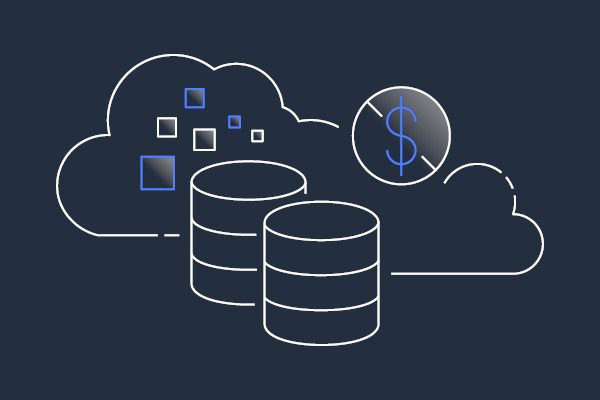
\includegraphics[scale = 0.70]{figs/db-logo-dollar}};

  \draw[comm] (t-alice) -- (t-alice |- isolation.north);
  \draw[comm] (t-bob) -- (t-bob |- isolation.north);
  \draw[comm] (t-carol) -- (t-carol |- isolation.north);
  \draw[comm] (isolation) -- (isolation |- db.north);

  \uncover<2->{
  \node[txn, below = 0.50cm of db, fill = green!30] (t-bob-execution)
    {$\readevent(\acctone, 60)$ \\[2pt]
     $\readevent(\accttwo, 60)$ \\[2pt]
     $\writeevent(\accttwo, -40)$};
  }
  \uncover<2->{
  \node[txn, left = of t-bob-execution] (t-alice-execution)
    {$\readevent(\acctone, 60)$ \\[2pt]
     $\readevent(\accttwo, 60)$ \\[2pt]
     $\writeevent(\acctone, -40)$};
  }
  \uncover<3->{
  \node[txn, right = of t-bob-execution, fill = red!30] (t-carol-execution)
    {$\readevent(\acctone, -40)$ \\[2pt]
     $\readevent(\accttwo, -40)$};

    \node[above = 1.50cm of t-carol-execution] (write-skew)
      {\green{\Large \textsc{Write Skew}}};
    \node[above = 0.80cm of t-carol-execution, scale = 3] (yes) {\yes};
  }
\end{tikzpicture}}

%     \vspace{0.20cm}
%     \violet{快照读性质:} 每个事务从它开始时的数据库{\it 快照}中读取数据
%   \end{center}
% \end{frame}
%%%%%%%%%%%%%%%%%%%%

%%%%%%%%%%%%%%%%%%%%
% \begin{frame}{}
%   \begin{center}
%     \red{快照隔离 (SI):} 弱于 SER, 但不允许\blue{\it 更新丢失}数据异常

%     \vspace{0.30cm}
%     \resizebox{0.48\textwidth}{!}{% isolation-si-lost-update-tikz.tex

\begin{tikzpicture}[
  node distance = 1.5cm and 1.5cm,
  txn/.style = {draw, inner sep = 3pt, align = center},
  comm/.style = {arrows = {Stealth-Stealth}, ultra thick, purple}]

  \node[txn] (t-alice)
    {$x \gets \readevent(\acct)$ \\[2pt]
     $x \gets x + 50$ \\[2pt]
     $\writeevent(\acct, x)$};

  \node[txn, right = of t-alice] (t-bob)
    {$x \gets \readevent(\acct)$ \\[2pt]
     $x \gets x + 25$ \\[2pt]
     $\writeevent(\acct, x)$};

  \node[txn, right = of t-bob] (t-carol)
    {$\readevent(\acct)$};

  \node[draw, fill = yellow!50, below = of t-bob, font = \large,
    inner sep = 8pt, minimum width = 260pt] (isolation)
    {{Snapshot Isolation (SI)}};

  \node[below = of isolation,
    label = {[label distance = 5pt]above : {\large $\acct = 0$}}] (db)
    {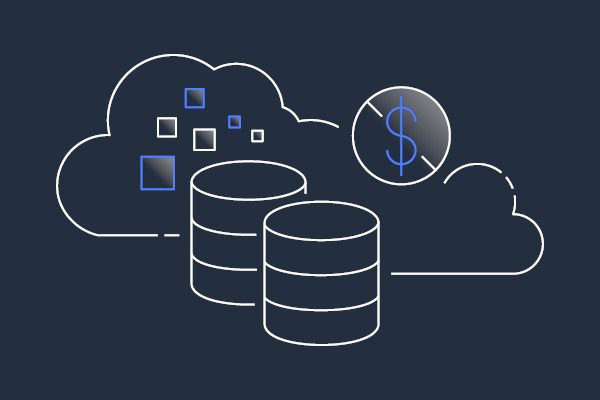
\includegraphics[scale = 0.70]{figs/db-logo-dollar}};

  \draw[comm] (t-alice) -- (t-alice |- isolation.north);
  \draw[comm] (t-bob) -- (t-bob |- isolation.north);
  \draw[comm] (t-carol) -- (t-carol |- isolation.north);
  \draw[comm] (isolation) -- (isolation |- db.north);

  \uncover<2->{
  \node[txn, below = 0.50cm of db] (t-bob-execution)
    {$\readevent(\acct, 0)$ \\[2pt] $\writeevent(\acct, ?)$};
  \node[below = 0.50cm of db, scale = 3.00] (t-bob-abort) {\no};
  }
  % \uncover<6->{
  % \node[txn, below = 0.50cm of db, fill = green!50] (t-bob-retry)
  %   {$\readevent(\acct, 0)$ \\[2pt] $\writeevent(\acct, 75)$};
  % }

  \uncover<2->{
  \node[txn, left = of t-bob-execution] (t-alice-execution)
    {$\readevent(\acct, 0)$ \\[2pt] $\writeevent(\acct, 50)$};
  }

  \uncover<2->{
  \node[above right = 0.20cm and 1.00cm of t-bob-execution] (lost-update)
    {\red{\large \textsc{Lost Update}}};
  \node[above right = -0.60cm and 1.30cm of t-bob-execution, scale = 3] (no) {\no};
  }
\end{tikzpicture}}
%   \end{center}

%   \vspace{-0.50cm}
%   \violet{快照写性质:}
%     并发事务之间不能存在写冲突; 最多只有一个可以提交
% \end{frame}
%%%%%%%%%%%%%%%%%%%%

%%%%%%%%%%%%%%%%%%%%
\begin{frame}{}
  \begin{center}
    事务一致性模型是数据库系统与上层业务之间的一种\red{\bf 契约}

    \vspace{0.30cm}
    \fig{width = 0.60\textwidth}{figs/layers}
  \end{center}
\end{frame}
%%%%%%%%%%%%%%%%%%%%

%%%%%%%%%%%%%%%%%%%%
\begin{frame}{}
  \begin{center}
    以\red{事务一致性模型}为核心的正确性问题至关重要

    \vspace{0.30cm}
    \fig{width = 0.60\textwidth}{figs/correctness}
  \end{center}
\end{frame}
%%%%%%%%%%%%%%%%%%%%

%%%%%%%%%%%%%%%%%%%%
\begin{frame}{}
  \fig{width = 0.65\textwidth}{figs/verification-problems}
\end{frame}
%%%%%%%%%%%%%%%%%%%%